% Options for packages loaded elsewhere
\PassOptionsToPackage{unicode}{hyperref}
\PassOptionsToPackage{hyphens}{url}
%
\documentclass[
  a5paper,
  smalldemyvopaper,10pt,twoside,onecolumn,openright,extrafontsizes,hidelinks]{memoir}

\usepackage{amsmath,amssymb}
\usepackage{iftex}
\ifPDFTeX
  \usepackage[T1]{fontenc}
  \usepackage[utf8]{inputenc}
  \usepackage{textcomp} % provide euro and other symbols
\else % if luatex or xetex
  \usepackage{unicode-math}
  \defaultfontfeatures{Scale=MatchLowercase}
  \defaultfontfeatures[\rmfamily]{Ligatures=TeX,Scale=1}
\fi
\usepackage{lmodern}
\ifPDFTeX\else  
    % xetex/luatex font selection
\fi
% Use upquote if available, for straight quotes in verbatim environments
\IfFileExists{upquote.sty}{\usepackage{upquote}}{}
\IfFileExists{microtype.sty}{% use microtype if available
  \usepackage[]{microtype}
  \UseMicrotypeSet[protrusion]{basicmath} % disable protrusion for tt fonts
}{}
\makeatletter
\@ifundefined{KOMAClassName}{% if non-KOMA class
  \IfFileExists{parskip.sty}{%
    \usepackage{parskip}
  }{% else
    \setlength{\parindent}{0pt}
    \setlength{\parskip}{6pt plus 2pt minus 1pt}}
}{% if KOMA class
  \KOMAoptions{parskip=half}}
\makeatother
\usepackage{xcolor}
\setlength{\emergencystretch}{3em} % prevent overfull lines
\setcounter{secnumdepth}{5}
% Make \paragraph and \subparagraph free-standing
\makeatletter
\ifx\paragraph\undefined\else
  \let\oldparagraph\paragraph
  \renewcommand{\paragraph}{
    \@ifstar
      \xxxParagraphStar
      \xxxParagraphNoStar
  }
  \newcommand{\xxxParagraphStar}[1]{\oldparagraph*{#1}\mbox{}}
  \newcommand{\xxxParagraphNoStar}[1]{\oldparagraph{#1}\mbox{}}
\fi
\ifx\subparagraph\undefined\else
  \let\oldsubparagraph\subparagraph
  \renewcommand{\subparagraph}{
    \@ifstar
      \xxxSubParagraphStar
      \xxxSubParagraphNoStar
  }
  \newcommand{\xxxSubParagraphStar}[1]{\oldsubparagraph*{#1}\mbox{}}
  \newcommand{\xxxSubParagraphNoStar}[1]{\oldsubparagraph{#1}\mbox{}}
\fi
\makeatother


\providecommand{\tightlist}{%
  \setlength{\itemsep}{0pt}\setlength{\parskip}{0pt}}\usepackage{longtable,booktabs,array}
\usepackage{calc} % for calculating minipage widths
% Correct order of tables after \paragraph or \subparagraph
\usepackage{etoolbox}
\makeatletter
\patchcmd\longtable{\par}{\if@noskipsec\mbox{}\fi\par}{}{}
\makeatother
% Allow footnotes in longtable head/foot
\IfFileExists{footnotehyper.sty}{\usepackage{footnotehyper}}{\usepackage{footnote}}
\makesavenoteenv{longtable}
\usepackage{graphicx}
\makeatletter
\def\maxwidth{\ifdim\Gin@nat@width>\linewidth\linewidth\else\Gin@nat@width\fi}
\def\maxheight{\ifdim\Gin@nat@height>\textheight\textheight\else\Gin@nat@height\fi}
\makeatother
% Scale images if necessary, so that they will not overflow the page
% margins by default, and it is still possible to overwrite the defaults
% using explicit options in \includegraphics[width, height, ...]{}
\setkeys{Gin}{width=\maxwidth,height=\maxheight,keepaspectratio}
% Set default figure placement to htbp
\makeatletter
\def\fps@figure{htbp}
\makeatother

% typographical packages
%\usepackage{microtype}
\usepackage{setspace}
%\tolerance=1000
%\hyphenpenalty=1000

% typographical settings for the body text
% \usepackage{microtype}
\DeclareMicrotypeAlias{stone-sans}{TU-basic}
\DeclareMicrotypeAlias{stone-serif}{TU-basic}
\raggedbottom

\setlength{\parskip}{0em plus 0em minus 0em}
%\setlength{\parindent}{1em}
\linespread{1.1}

% DEFINITIONS TITLE PAGE / COPYRIGHT
\newcommand{\titleoriginal}{Broken Money}
\newcommand{\subtitleoriginal}{Why Our Financial System is Failing Us and How We Can Make it Better}
\newcommand{\yearoriginal}{2023}
\newcommand{\subtitletranslation}{XXX}
\newcommand{\yeartranslation}{2025}
\newcommand{\stringtranslation}{Traduzione}
\newcommand{\stringlicense}{Tutti i diritti riservati.}
\newcommand{\stringpublisher}{Pubblicato da}
\newcommand{\ISBNHC}{XXX}
\newcommand{\ISBNSC}{XXX}
\newcommand{\ISBNEBOOK}{XXX}
\newcommand{\ISBNAUDIO}{XXX}
\newcommand{\press}{Konsensus Network}
\newcommand{\translatorone}{XXX}
\newcommand{\translatortwo}{XXX}
\newcommand{\translators}{
\Large\sffamily\textbf{\stringtranslation:}\\
\textit\translatorone\\
\textit\translatortwo\\
}
\newcommand{\editors}{
  \Large\sffamily\textbf{Redactie:}\\
  \textit{Theo Hague}
}

% PHYSICAL DOCUMENT SETUP
\setstocksize{230mm}{155mm}
\settrimmedsize{224mm}{149mm}{*}
\setbinding{7mm}
\setlrmarginsandblock{15mm}{18mm}{*}
\setulmarginsandblock{20mm}{18mm}{*}

% FONTS
\usepackage{fontspec}
\setmainfont{stone-serif}[
    Path=./fonts/stone-serif-itc-pro/,
    Scale=0.90,
    Extension=.OTF,
    UprightFont=*-Regular,
    BoldFont=*-SemiBd,
    ItalicFont=*-MediumIt,
    BoldItalicFont=*-SemiBdIt
    ]

\setsansfont{stone-sans}[
    Path=./fonts/stone-sans/,
    Scale=0.85,
    Extension=.otf,
    UprightFont=*-Medium,
    BoldFont=*-Semibold,
    ItalicFont=*-MediumItalic,
    BoldItalicFont=*-SemiBoldItalic
    ]

\setmonofont{Consolas}

% Define a new font family for chapter headings using XeLaTeX and fontspec.
\newfontfamily\chapterfont{Portmanteau-Regular}[
    Path=./fonts/,
    Scale=0.8,
    Extension=.otf,
]

\newfontfamily\quotefont{stone-sans-Regular}[
    Path=./fonts/stone-sans/,
    Scale=0.85,
    Extension=.ttf,
]

\newfontfamily\titlefont{delight-bold}[
    Path=./fonts/,
    Scale=0.85,
    Extension=.otf,
]

% Define YUGE
\newcommand{\YUGE}{\fontsize{36pt}{43pt}\selectfont}
\newcommand{\Yuge}{\fontsize{30pt}{36pt}\selectfont}
\newcommand{\yuge}{\fontsize{27pt}{32pt}\selectfont}

% Lettrine chapter opening global settings
\usepackage{lettrine}
\setcounter{DefaultLines}{2}
\renewcommand{\DefaultLoversize}{0.1}
\renewcommand{\DefaultLraise}{0}
\renewcommand{\LettrineTextFont}{}
\setlength{\DefaultFindent}{\fontdimen2\font}
\setlength{\DefaultNindent}{0em}

% Endnotes
\usepackage{enotez}
% \let\footnote=\endnote
% \let\footnotemark=\endnotemark
% \let\footnotetext=\endnotetext
\setenotez{
  list-name={Eindnoten},
  reset=true,
  backref=true,
}

% custom second title page
\makeatletter
\newcommand*\halftitlepage{\begingroup
  \setlength\drop{0.1\textheight}
  \begin{center}
  \vspace*{\drop}
  \rule{\textwidth}{0in}\par
  {\Yuge\titlefont\MakeUppercase{\thetitle}\par}
  \rule{\textwidth}{0in}\par
  \vfill
  \end{center}
\endgroup}
\makeatother

% custom title page
\makeatletter
\newlength\drop
\newcommand*\titleM{\begingroup % Misericords, T&H p 153
  \setlength\drop{0.15\textheight}
  \begin{center}
  \vspace*{\drop}
  {\Huge\sffamily\MakeUppercase{\theauthor}\par}
  \vspace{3em}
  {\YUGE\titlefont\MakeUppercase{\thetitle\par}}
  \vspace{8em}
  \begin{minipage}{0.8\textwidth}
    {\LARGE\centering\sffamily\textit\subtitletranslation\par}
  \end{minipage}
  \par
  % \rule{5.5cm}{0.3mm}\par
  \vspace{12em}
  {\footnotesize\translators\par}
  \vspace{2em}
  {\footnotesize\editors\par}
  \vfill
  % \includegraphics[width=3.5cm]{figures/knw.png}\par
  \end{center}
\endgroup}
\makeatother

% copyright page
\makeatletter
\newcommand*\copyrightpage{\begingroup
  \setlength\drop{0.1\textheight}
  \vphantom{just for the drop}
  \vfill
  \begin{footnotesize}
  \noindent \copyright\space \yearoriginal: \theauthor
  \par\noindent \textit{\titleoriginal: \subtitleoriginal}
  \vspace{0.5\baselineskip}
  \par\noindent \copyright\space \yeartranslation\space \stringtranslation: \translatorone, \space \translatortwo
  \par\noindent \textit{\thetitle: \subtitletranslation}
  \vspace{\baselineskip}
  \par\noindent \textit{\stringlicense}
  \vspace{0.5\baselineskip}
  \par\noindent \stringpublisher: \href{https://konsensus.network}{\textit{konsensus.network}}
  \vspace{0.5\baselineskip}
  \par\noindent Impaginazione: Theo Hague
  \vspace{0.5\baselineskip}
  \par\noindent Design di copertina: Imtechnicolor
  \vspace{0.5\baselineskip}
  \par\noindent Prima edizione: maggio 2025
  \vspace{0.5\baselineskip}
  \setlength{\parindent}{2em}% default 20pt
  \par\noindent ISBN \ISBNHC \:Hardcover
  \par\hspace{0.28\parindent}\ISBNSC \:Paperback
  \par\hspace{0.28\parindent}\ISBNEBOOK \:E-book\par
  \setlength{\parindent}{0pt}
  \end{footnotesize}
  \vspace{3em}
  % \par\noindent \href{https://konsensus.network}{\large\MakeUppercase \press \hspace{3em} \includegraphics[width=1cm]{figures/freestarfish.png}}
  \includegraphics[width=3.5cm]{figures/knw.png}\par
  \setcounter{footnote}{0}
  \clearpage
\endgroup}
\makeatother

% HEADER AND FOOTER MANIPULATION
% for normal pages
\nouppercaseheads
\headsep = 6mm
\makepagestyle{mystyle} 
\makeevenhead{mystyle}{\footnotesize\sffamily\thepage}{}{}
\makeoddhead{mystyle}{{\footnotesize\sffamily\leftmark}}{}{\footnotesize\sffamily\thepage}
\makeevenfoot{mystyle}{}{}{}
\makeoddfoot{mystyle}{}{}{}
\makeatletter

% for pages where chapters begin
\makepagestyle{plain}
\makerunningwidth{plain}{\headwidth}
\makeevenfoot{plain}{}{}{}
\makeoddfoot{plain}{}{}{}
\pagestyle{mystyle}

% \newif\ifmainmatter
% \appto\mainmatter{\mainmattertrue}
% \appto\backmatter{\mainmatterfalse}
% \appto\appendix{\mainmatterfalse}

% \renewcommand\chaptermark[1]{%
%   \markboth{\MakeUppercase{%
%     \ifmainmatter~\oldstylenums\thechapter.~\fi#1}}{}}%

% TOC
\usepackage[]{tocloft}
\renewcommand{\cftsectiondotsep}{\cftnodots}
\renewcommand{\cftpartfont}{\Large\sffamily\MakeUppercase}
\renewcommand{\cftchapterfont}{\normalsize\sffamily}
\renewcommand{\cftsectionfont}{\Small\sffamily}
\renewcommand{\cftpartpagefont}{\Large\sffamily}
\renewcommand{\cftchapterpagefont}{\small}
\renewcommand{\cftchapterpresnum}{CAPITOLO\space}
\renewcommand{\cftchapternumwidth}{8em}
\setlength{\cftchapterindent}{0em}
\setlength{\cftsectionindent}{8em}
\setlength{\cftbeforechapterskip}{0.4em}
\setsecnumdepth{chapter}
\setcounter{tocdepth}{0}

%% Some spacing between the last chapter and the backmatter
\pretocmd{\backmatter}{\addtocontents{toc}{\vspace{2em}}}{}{}


% Redefine footnote presentation
\makeatletter
\renewcommand\@makefntext[1]{%
  \noindent\hb@xt@2em{% <-- Box of fixed size for footnote number and space
    \@thefnmark\quad}% <-- Footnote number followed by a quad space
  \parbox[t]{\dimexpr\linewidth-2em}{#1}% <-- Parbox to control the width of footnote content
}
\makeatother

% layout check and fix
\checkandfixthelayout

% COUNTERS FOOTNOTES
\usepackage{chngcntr}
\counterwithout*{footnote}{chapter}

% CAPTIONS
\usepackage[format=plain,labelsep=newline,font=small,labelfont={bf,sf},singlelinecheck=false]{caption}

% TITLE FORMATTING
\usepackage{titlesec}
\titleclass{\part}{top}
\titleformat{\part}[display]
  {\sffamily\Huge}
  {\chapterfont\centering\partname\ \thepart}
  {2em}
  {\HUGE\centering\uppercase}
%\titlespacing*{\part}{0pt}{50pt}{40pt}

\titleformat
    {\chapter}[display]
    {\huge\sffamily}
    {\huge\sffamily\chaptertitlename\space\thechapter}
    {1em}
    {}

\titleformat
{\section}[block]
{\sffamily\Large}
{}
{0pt}
{\uppercase}
  
\titlespacing*{\section}{0pt}{2em}{0.5em}

\titleformat{\subsection}{\sffamily\large\bfseries}{}{}{\uppercase}
%\titlespacing*{\subsection}{0pt}{2em}{0em}

\makeatletter
\renewcommand*{\@makechapterhead}[1]{%
  %\linespread{1.3}
  \vspace*{-4cm} % Adjust vertical spacing before the image
  \begin{center}
    \setSpacing{1.3}
    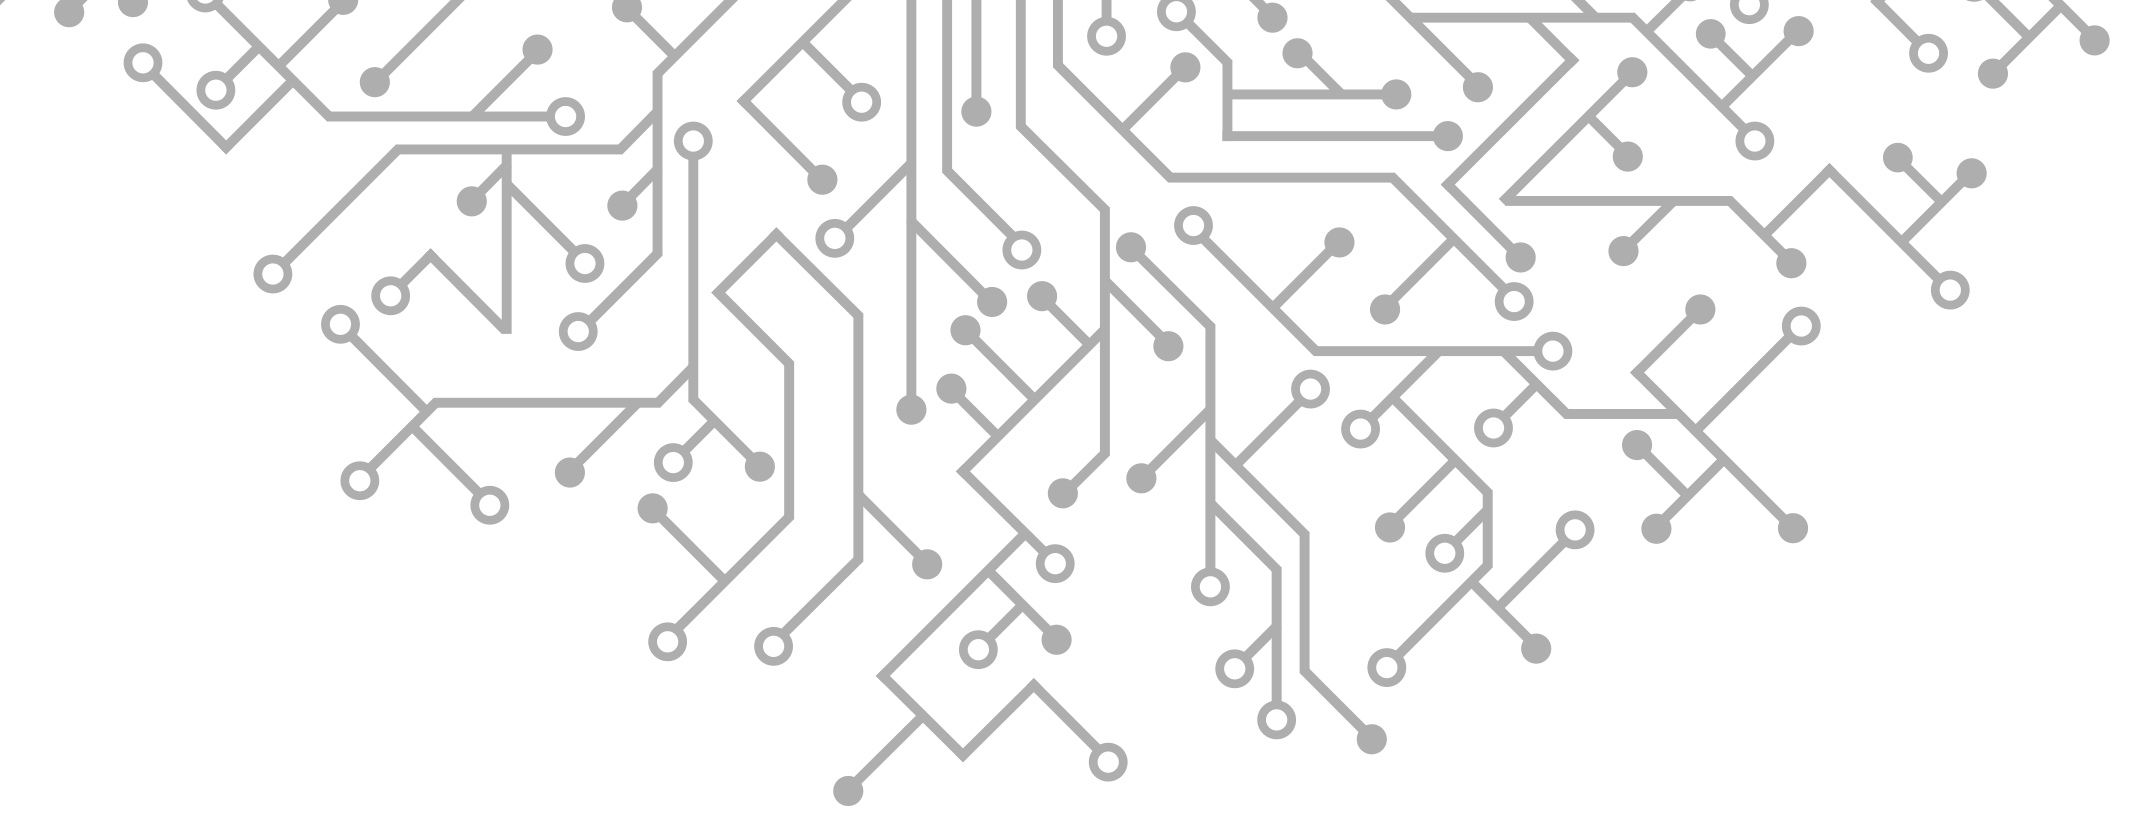
\includegraphics[width=\textwidth]{figures/circuitboard.png}
    \par\vspace{3\baselineskip} % Add reliable spacing after the image
    {\LARGE\chapterfont Capitolo \thechapter} 
    \par\vspace{1\baselineskip} % Space before chapter number
    {\huge\sffamily\MakeUppercase{#1}} % Chapter title formatting
    \par\vspace{1\baselineskip} % Space after chapter number
  \end{center}
  \vspace{2\baselineskip} % Space after the chapter title
}
\makeatother


% QUOTE FORMATTING
\renewenvironment{quote}%
               {\list{}{\rightmargin=1.5em\leftmargin=1.5em\topsep=1.5em\itemindent=0em}%
                 \small \item[]\relax}% <- The effect of \samepage is local!!!
               {\endlist}

% LAYOUT CHECK AND FIX
\checkandfixthelayout

% CUSTOM TITLE PAGE
\makeatletter
\def\@maketitle{%
  % the half title page
  \pagestyle{empty}
  \halftitlepage
  \cleardoublepage

  % the title page
  \titleM
  \clearpage

  % the copyright page
  \copyrightpage
  \cleardoublepage
  \pagestyle{mystyle}
}
\makeatother
% END PREAMBLE
\makeatletter
\@ifpackageloaded{bookmark}{}{\usepackage{bookmark}}
\makeatother
\makeatletter
\@ifpackageloaded{caption}{}{\usepackage{caption}}
\AtBeginDocument{%
\ifdefined\contentsname
  \renewcommand*\contentsname{Indice}
\else
  \newcommand\contentsname{Indice}
\fi
\ifdefined\listfigurename
  \renewcommand*\listfigurename{Elenco delle Figure}
\else
  \newcommand\listfigurename{Elenco delle Figure}
\fi
\ifdefined\listtablename
  \renewcommand*\listtablename{Elenco delle Tabelle}
\else
  \newcommand\listtablename{Elenco delle Tabelle}
\fi
\ifdefined\figurename
  \renewcommand*\figurename{Figura}
\else
  \newcommand\figurename{Figura}
\fi
\ifdefined\tablename
  \renewcommand*\tablename{Tabella}
\else
  \newcommand\tablename{Tabella}
\fi
}
\@ifpackageloaded{float}{}{\usepackage{float}}
\floatstyle{ruled}
\@ifundefined{c@chapter}{\newfloat{codelisting}{h}{lop}}{\newfloat{codelisting}{h}{lop}[chapter]}
\floatname{codelisting}{Lista}
\newcommand*\listoflistings{\listof{codelisting}{Elenco degli Elenchi}}
\makeatother
\makeatletter
\makeatother
\makeatletter
\@ifpackageloaded{caption}{}{\usepackage{caption}}
\@ifpackageloaded{subcaption}{}{\usepackage{subcaption}}
\makeatother

\ifLuaTeX
\usepackage[bidi=basic]{babel}
\else
\usepackage[bidi=default]{babel}
\fi
\babelprovide[main,import]{italian}
% get rid of language-specific shorthands (see #6817):
\let\LanguageShortHands\languageshorthands
\def\languageshorthands#1{}
\ifLuaTeX
  \usepackage{selnolig}  % disable illegal ligatures
\fi
\usepackage{bookmark}

\IfFileExists{xurl.sty}{\usepackage{xurl}}{} % add URL line breaks if available
\urlstyle{same} % disable monospaced font for URLs
\hypersetup{
  pdftitle={Book Title},
  pdfauthor={Book Author},
  pdflang={it},
  hidelinks,
  pdfcreator={LaTeX via pandoc}}


\title{Book Title}
\author{Book Author}
\date{+0100-01-01}

\begin{document}
\frontmatter
\maketitle

\renewcommand*\contentsname{Indice}
{
\setcounter{tocdepth}{0}
\tableofcontents
}

\mainmatter
\bookmarksetup{startatroot}

\chapter*{Over dit boek}\label{over-dit-boek}
\addcontentsline{toc}{chapter}{Over dit boek}

\markboth{Over dit boek}{Over dit boek}

\bookmarksetup{startatroot}

\chapter*{Introduzione}\label{introduzione}
\addcontentsline{toc}{chapter}{Introduzione}

\markboth{Introduzione}{Introduzione}

A settembre 2022, un'ondata di persone comuni ha rapinato banche in
Libano.

Ciò che ha resa questi eventi più degni di notizia rispetto alle tipiche
rapine in banca è stato il fatto che la maggior parte di queste persone
stava rapinando le banche per riavere indietro il \emph{proprio denaro}.
A causa di una crisi finanziaria in Libano, infatti, le banche non
permettevano alle persone di accedere ai propri depositi in contanti per
lungo tempo.

Una delle ``rapinatrici di banche'' che ha fatto notizia era una giovane
donna che lavorava come interior decorator. Ha rapinato una banca a
Beirut usando quella che in seguito si è rivelata essere una pistola
finta dall'aspetto estremamente realistico, con l'intento di prelevare i
risparmi della sua famiglia destinati al trattamento della sorella,
afflitta dal cancro, poiché i risparmi erano stati congelati dalla
banca. Questo è stato forse l'esempio più eclatante, ma ci furono anche
altre rapine durante quel periodo, effettuate da persone che volevano
semplicemente riavere indietro i propri depositi, e alcune di esse
ricorsero anche ad armi reali.

Questi eventi in Libano sono specifici di un determinato paese e momento
storico, ma fanno parte di una storia globale.

Nigeria, un paese con oltre 200 milioni di abitanti, ha registrato
un'inflazione annualizzata del 13\% nell'ultimo decennio.\footnote{FMI,
  ``Prezzi al consumo, fine periodo,'' Datamapper.} Nel 2021 è stata
lanciata una valuta digitale della banca centrale, la eNaira, che finora
ha riscosso un'adozione estremamente bassa, mentre le criptovalute (in
particolare bitcoin e stablecoin ancorate al dollaro statunitense) hanno
registrato un tasso di adozione superiore di un ordine di grandezza
all'interno del paese, pur essendo escluse dal sistema bancario
nazionale. Il governo nigeriano ha successivamente adottato una serie di
politiche volte a ridurre la disponibilità di contante fisico e a
spingere la popolazione verso i pagamenti digitali, contribuendo così a
un periodo di sconvolgimenti politici e a sommersi scontri.

L'Egitto ha improvvisamente dimezzato il valore della propria valuta
rispetto al dollaro statunitense nell'autunno del 2016, compromettendo
anni di risparmi per una popolazione di circa 100 milioni di abitanti.
Nel 2022 e nel 2023 il paese ha nuovamente effettuato diverse brusche
devalutazioni della propria valuta rispetto al dollaro, portando a un
ulteriore dimezzamento del tasso di cambio. Conosco persone in Egitto
che acquistano dollari fisici sul mercato nero e li detengono come
protezione contro questo problema persistente. Pagano commissioni di
conversione considerevoli per farlo, senza però ottenere interessi sui
dollari cartacei detenuti. E quando tali devalutazioni si verificano,
ricade immediatamente su tutti i lavoratori del paese l'onere di cercare
di negoziare stipendi più alti per recuperare parte del potere
d'acquisto perso, poiché i loro salari continuativi sono espressi nella
valuta locale deprezzata.

La Turchia e l'Argentina, entrambi membri delle nazioni del G20 e con
una popolazione complessiva di oltre 130 milioni di abitanti, hanno
dovuto far fronte a un'inflazione incontrollata negli ultimi anni. La
Turchia ha raggiunto un'inflazione anno su anno dell'85\% nel 2022,
mentre l'Argentina ha superato il 100\% di inflazione nel
2023.\footnote{Zeynep Dierks, ``Tasso di inflazione CPI in Turchia,''
  \emph{Statista}, 3 marzo 2023;
  \href{https://www.bloomberg.com/authors/ATpJM4rxzpI/patrick-gillespie}{Patrick~Gillespie},
  ``L'inflazione in Argentina supera il 100\% mentre incombe una
  recessione economica,'' \emph{Bloomberg}, 14 marzo 2023.}

Negli anni '90 il Brasile sperimentò una vera iperinflazione, essendo
allora il quinto paese più popoloso del mondo. Quando si immagina
l'iperinflazione, spesso ci si riferisce alla Germania degli anni '20 o
ad alcuni stati falliti contemporanei, ma un numero sorprendentemente
elevato di paesi l'ha vissuta in un determinato periodo durante la
seconda metà del XX secolo. Già dagli anni '80 in poi, persone in
Brasile, Argentina, Jugoslavia, Zimbabwe, Venezuela, Polonia,
Kazakistan, Perù, Bielorussia, Bulgaria, Ucraina, Libano e altri hanno
sperimentato l'iperinflazione. Altri paesi, come Israele, Messico,
Vietnam, Ecuador, Costa Rica e la Turchia, hanno avuto un'inflazione a
tre cifre (cioè quasi iperinflazione) in quel periodo.

Dal 2016 al 2021, molti mercati obbligazionari di nazioni ricche in
Europa e in Giappone offrivano rendimenti nominali prossimi allo zero o
addirittura negativi, con oltre 18 trilioni di dollari in obbligazioni a
rendimento negativo al picco.\footnote{Cormac Mullen e John Ainger,
  ``L'ammasso mondiale di debito a rendimento negativo raggiunge il
  record di 18 trilioni di dollari,'' \emph{Bloomberg}, 11 dicembre
  2020.} Le persone dovevano pagare per il privilegio di prestare denaro
a governi e grandi imprese, invece di guadagnare interessi. Di
conseguenza, gli incentivi del sistema finanziario furono completamente
rovesciati. Nei successivi anni, tuttavia, un'ondata globale di
inflazione ridusse drasticamente il potere d'acquisto dei detentori di
tali obbligazioni.

Negli anni 2010, diversi alti funzionari della Federal Reserve
statunitense hanno ripetutamente dichiarato che l'economia era troppo a
lungo al di sotto del loro obiettivo medio di inflazione e che
desideravano un'inflazione più alta. Durante un'udienza congressuale
all'inizio del 2021, quando il tasso di inflazione principale negli
Stati Uniti era dell'1,7\%, un deputato chiese al presidente della
Federal Reserve riguardo all'incremento del 25\% su base annua
dell'aggregato monetario (il più alto dagli anni '40) avvenuto a seguito
dei recenti stimoli fiscali, e alle eventuali implicazioni che ciò
potesse avere sull'inflazione o sul valore del dollaro. Il presidente
respinse tali preoccupazioni, affermando che un tale aumento
dell'aggregato monetario probabilmente non avrebbe avuto importanti
conseguenze economiche e che forse sarebbe stato necessario
``dimenticare'' l'idea che gli aggregati monetari abbiano un impatto
rilevante sull'economia.\footnote{Howard Schneider, ``Powell's Econ 101:
  posti di lavoro, non inflazione. E dimenticate l'offerta di moneta,''
  \emph{Reuters}, 23 febbraio 2021.}

Quando, verso la fine del 2021, l'inflazione dei prezzi iniziò a
manifestarsi seriamente, il presidente la liquidò inizialmente come
transitoria e la Federal Reserve continuò ad espandere la base monetaria
attraverso il quantitative easing. Ma poi, con il verificarsi nel 2022
di tassi d'inflazione ai massimi di quattro decenni, il presidente e
altri leader della Federal Reserve entrarono in panico e cambiarono
completamente la loro politica monetaria, individuando l'inflazione dei
prezzi come il problema più urgente da affrontare. Nel tentativo di
domare l'inflazione, aumentarono i tassi in modo così aggressivo --- e
ridussero la base monetaria a un ritmo record nell'anno successivo ---
da finire per creare perdite non realizzate per le banche per un valore
superiore a un trilione di dollari sui loro titoli del Tesoro e su altri
asset a basso rischio. Estraendo depositi dal sistema bancario a un
ritmo così sostenuto, contribuirono ad alcune delle maggiori crisi
bancarie della storia americana. Entro il 2023, le banche di tutto il
paese avevano rapporti di capitale gravemente compromessi a causa
dell'impennata dei tassi di interesse. Per la prima volta nella storia
moderna, persino la Federal Reserve registrava una perdita operativa,
dovuta al pagamento di tassi così elevati sulle proprie passività
rispetto a quanto guadagnato sugli asset.\footnote{Erica Jiang et al.,
  ``Rafforzamento monetario e fragilità delle banche statunitensi nel
  2023.''} Queste decisioni della Federal Reserve influenzano le
condizioni monetarie per 330 milioni di americani e per miliardi di
persone all'estero, eppure vengono prese manualmente e soggettivamente
da un gruppo di sole dodici persone.

Esistono circa 160 valute diverse nel mondo,\footnote{XE.com. ``Codici
  ISO 4217 delle valute.''} ciascuna con un monopolio locale all'interno
della propria giurisdizione, e la maggior parte di esse ha poca o
nessuna accettazione fuori dai propri confini. L'ordine finanziario
globale è, a questo proposito, praticamente un sistema di baratto. Una
manciata di valute principali sono detenute come riserve da altre banche
centrali e godono di un certo grado di accettazione internazionale, ma
perdono valore lentamente nel tempo e i loro tassi d'interesse non hanno
seguito l'inflazione per anni. La maggior parte delle altre valute è
invece più soggetta a brusche svalutazioni, a periodi persistenti di
inflazione a doppia cifra e a occasionali iperinflazioni, pur godendo di
scarsa o nessuna accettazione estera. Per le persone che vivono in
questi paesi, spesso si cerca di procurarsi valute straniere, come il
dollaro, per proteggere i propri risparmi, poiché generalmente non ci si
può fidare delle banche locali per custodirli.

Risparmiare denaro può essere una sfida anche nelle giurisdizioni
monetarie più stabili, e se qualcuno nasce nella ``giurisdizione
sbagliata'', la battaglia per mettere da parte denaro diventa
incredibilmente ardua.

Come siamo arrivati a questo punto? Perché il nostro denaro non è
\emph{meglio} di così?

Il sistema finanziario globale si è dimostrato inadeguato per i paesi in
via di sviluppo lungo tutta la storia moderna e, nelle ultime decadi, ha
accumulato seri squilibri anche nei paesi sviluppati. Le sue fondamenta
non risultano più solide, in parte perché la tecnologia di base è
obsoleta.

Sostengo che l'ascesa del populismo negli Stati Uniti, in Europa e in
numerosi paesi in via di sviluppo, a partire dalla crisi finanziaria
globale del 2008, sia in larga misura attribuibile a questo fatto.
Persone di sinistra e di destra percepiscono che qualcosa non va, che il
sistema è ``truccato'' contro di loro, ma non riescono a comprendere
esattamente il motivo. Un tassello fondamentale di questo enigma è
rappresentato dal fatto che il sistema finanziario, come lo conosciamo,
non funziona più.

Abbiamo visto, nelle decadi passate, come gli ordini finanziari globali
si disintegrino gradualmente a causa dell'accumulo di squilibri
economici, del verificarsi di riallineamenti geopolitici e
dell'introduzione di nuove tecnologie. Quando ciò accade, il vecchio
ordine viene in parte o completamente ricostruito, dando vita a un nuovo
assetto, come si può osservare in numerosi esempi riportati in questo
libro. Tutti gli indizi suggeriscono che l'ordine finanziario vigente
dagli anni '70 stia giungendo ai suoi ultimi anni e stia avviando un
processo di ricostruzione e riallineamento.

Questo è un libro sul denaro esaminato attraverso la lente degli
sviluppi tecnologici. Esso analizza l'evoluzione del denaro nel passato,
il motivo per cui le tecnologie e le istituzioni attuali dedicate al
denaro non ci soddisfano più e alcune delle possibili soluzioni ai
problemi monetari che oggi affrontiamo. È scritto in un linguaggio
semplice ed è strutturato in moduli, così che i lettori possano
concentrarsi sulle parti che più li interessano.

\textbf{Parte 1} del libro accompagna il lettore attraverso antichi
registri contabili e forme di denaro merce, per analizzare perché il
denaro sia emerso in maniera naturale e perché alcune forme di denaro
abbiano prevalso su altre. Questo percorso ci aiuta a discernere quali
siano le proprietà ideali del denaro e perché tali proprietà tendano a
riemergere in maniera indipendente nel corso della storia. Esamina
inoltre il rapporto tra credito sociale e denaro merce, offrendo un
punto di convergenza tra due scuole economiche spesso in contrasto.

\textbf{Parte 2} parla dei primi servizi proto-bancari e dell'ascesa
delle banche a servizio completo. Esamina come vari sviluppi tecnologici
abbiano accelerato le transazioni monetarie e le abbiano disgiunte dal
più lento processo dei regolamenti fisici, comportando numerosi benefici
ma anche alcuni svantaggi. Conclude illustrando come il divario
crescente tra la rapidità delle transazioni e quella dei regolamenti,
all'alba dell'era delle telecomunicazioni, abbia conferito un notevole
potere a banche e banche centrali, divenute le entità primarie capaci di
trasmettere denaro in fretta in tutto il mondo.

\textbf{Parte 3} descrive il sistema finanziario globale così come è
stato strutturato fin dai primi del Novecento, includendo la geopolitica
alla base della sua creazione e il suo evolversi nel tempo. Copre il
periodo dei fallimenti dei peg in oro intorno alla Prima Guerra
Mondiale, il sistema di Bretton Woods, esistito dagli anni '40 agli
inizi degli anni '70, e il sistema Eurodollaro/Petrodollaro che lo ha
sostituito dagli anni '70 fino ai giorni nostri. Infine, spiega come
alcuni aspetti problematici dell'attuale versione del sistema abbiano
condotto a squilibri strutturali in tutto il mondo negli ultimi decenni.

\textbf{Parte 4} analizza in dettaglio come il denaro venga creato nel
moderno sistema finanziario e come il debito, per sua natura,
destabilizzi il sistema nel tempo. Esamina, inoltre, alcuni degli
squilibri e degli incentivi problematici causati dalla costante
svalutazione delle unità monetarie, mentre i risparmiatori cercano di
preservarne il potere d'acquisto acquistando altri asset non monetari.
Mostra come i legislatori siano stati dotati di un registro pubblico
flessibile, che consente loro di intraprendere guerre senza ricorrere
alla tassazione, di effettuare salvataggi selettivi tramite la
svalutazione dei risparmi altrui e, in generale, di finanziare spese in
modo opaco.

\textbf{Parte 5} esamina le innovazioni monetarie digitali del XXI
secolo, includendo Bitcoin, stablecoin, smart contract e le valute
digitali delle banche centrali. Questa è la parte più speculativa del
libro, in quanto tratta del presente e del futuro piuttosto che del
passato. Descrive alcune delle nuove tecnologie a nostra disposizione e
analizza nello specifico i vari compromessi e rischi connessi a queste
tecnologie, accanto alle opportunità che esse possono offrire.

\textbf{Parte 6} esplora l'etica del denaro e della comunicazione, che
rappresentano le due componenti fondamentali del commercio. Discute il
ruolo della crittografia in generale (un elemento cruciale per il
moderno sistema bancario e l'infrastruttura di internet), il confronto
tra reti finanziarie aperte e chiuse, e l'intersezione tra tecnologia
finanziaria e diritti umani.

Fondamentalmente, il denaro è un registro contabile. Il denaro-merce
funge da registro governato dalla natura. Il denaro bancario è un
registro controllato dagli stati nazionali. Il denaro open-source è un
registro gestito dagli utenti. Come esplora il libro, l'evoluzione della
tecnologia cambia le strutture di potere e gli incentivi che circondano
il denaro da un'epoca all'altra.

Il mio percorso professionale unisce ingegneria e finanza, e adotto un
approccio di ingegneria dei sistemi per analizzare vari aspetti del
sistema finanziario globale. L'ingegneria dei sistemi è un campo
multidisciplinare che si concentra sulla progettazione,
sull'integrazione, sul funzionamento e sulla manutenzione di sistemi
complessi nel corso del loro ciclo di vita. Considero il sistema
finanziario globale come il vero sistema ingegnerizzato che è, e ho
constatato che questo metodo di analisi porta a conclusioni innovative
che a volte sfidano il pensiero economico convenzionale.

Il mio obiettivo nel scrivere questo libro è aiutare le persone a
comprendere meglio come funziona il denaro e perché il sistema
finanziario globale non operi più come una volta. Il libro non tratta
esclusivamente del perché il nostro sistema finanziario non funzioni
bene quest'anno o in questo decennio, ma rappresenta un'analisi più
profonda su cosa sia il denaro, su come siamo arrivati alla situazione
attuale e su quali siano i problemi fondamentali attuali.

Non ho tutte le risposte e non posso prevedere come sarà il mondo della
finanza nei prossimi decenni, ma con questo libro intendo condividere le
mie ricerche affinché i lettori possano trovare ulteriori risposte per
conto proprio. La politica può influenzare le cose in maniera locale e
temporanea, ma la tecnologia ha effetti globali e permanenti; per questo
motivo analizzo il denaro prevalentemente attraverso la lente della
tecnologia.

Questo non è un libro sull'oro, né un libro bancario, né un libro sul
bitcoin, né un libro politico. È, invece, un'esplorazione delle
tecnologie monetarie nelle loro innumerevoli forme -- passate, presenti
e future -- che tocca tutti questi temi e oltre, affinché possiamo
comprendere meglio da dove veniamo e quali percorsi potremmo
intraprendere in futuro.

\part{Cos'è il denaro?}

\chapter*{Part 1}\label{part-1}
\addcontentsline{toc}{chapter}{Part 1}

\markboth{Part 1}{Part 1}

``I precursori del denaro, insieme al linguaggio, permisero agli esseri
umani della prima età moderna di superare le problematiche cooperative
che altre specie non sono in grado di risolvere --- tra cui l'altruismo
reciproco, l'altruismo filiale e la mitigazione dell'aggressività. Tali
precursori condividevano con le valute non fiat una serie di
caratteristiche molto specifiche --- non erano meri oggetti simbolici o
decorativi.''\footnote{Nick Szabo, \emph{Shelling Out: The Origins of
  Money.}}

-Nick Szabo

\chapter{I registri come fondamento del
denaro}\label{i-registri-come-fondamento-del-denaro}

Molti pensano che il concetto di denaro nasca con l'introduzione delle
monete o delle conchiglie, ma in realtà la storia comincia ben prima,
precisamente con l'idea di un registro contabile.

Un registro, inteso come riepilogo delle transazioni, serve a tenere
traccia dei rapporti di proprietà. I più antichi registri scritti, sotto
forma di tavolette di argilla, risalgono a oltre 5.000 anni fa nella
Mesopotamia antica. Secondo l'Encyclopedia Britannica, il sumero
rappresenta il più antico sistema di scrittura conosciuto, e le
testimonianze più antiche di questa scrittura sono proprio registri
cuneiformi che annotavano il passaggio di merci\footnote{Ignace Gelb,
  ``Sumerian Language.''}. Su queste tavolette figuravano
rappresentazioni pittoriche di vari beni, accompagnate da puntini
indicanti le quantità, i quali costituivano le prime forme di
elencazione della proprietà, del credito o delle transazioni, così come
li sappiamo dai protoscritti degli albori della civiltà\footnote{William
  Goetzmann, \emph{Money Changes Everything: How Finance Made
  Civilization Possible}, 15--25.}.

Il concetto di registro, tuttavia, può essere inteso in termini ancora
più semplici. Anche prima dell'invenzione della scrittura, nei meandri
della memoria e della tradizione orale, esisteva una forma primitiva di
registro. Ogni volta che qualcuno si trovava in debito, formalmente o
meno, con un altro soggetto, veniva così creato, implicitamente, un
registro orale di obblighi e scambi.

A titolo esemplificativo, immaginiamo una situazione contemporanea: due
fratelli, Alice e Bobby, abbastanza grandi da occuparsi di faccende
domestiche, che talvolta devono organizzare i loro impegni. Ad esempio,
Alice potrebbe avere necessità di rinunciare alle faccende una sera per
uscire con gli amici e, per rimediare, proporre a Bobby di occuparsi
delle sue faccende quel giorno in cambio del fatto che lei si faccia
carico delle sue il giorno seguente. Accettando l'accordo, i due creano
così un semplice registro mentale -- una forma basica di credito -- in
cui Alice accumula un debito nei confronti di Bobby relativo a
specifiche faccende. Tale accordo si basa unicamente sulla fiducia e
sulla reputazione: se Alice non adempie al suo debito, Bobby tenderà a
rifiutare futuri scambi. In situazioni semplici il registro rimane
puramente verbale, ma se gli impegni diventano complessi e le faccende
vengono scambiate regolarmente, potrebbe essere utile ricorrere a un
calendario, trasformando il registro in un documento scritto. In questo
contesto non esiste un'unità monetaria specifica: si tratta
semplicemente di un sistema di baratto, in cui le ``unità'' sono
costituite dalle faccende stesse, e il registro è impiegato per tenere
traccia degli scambi nel tempo, fungendo da strumento di credito.

Possiamo immaginare, ad esempio, un gruppo di cacciatori, magari decine
di migliaia di anni fa in una tribù qualsiasi, che contava il numero
delle prede abbattute o che teneva in maniera sommaria il conto dei
favori scambiati. Le tribù di tutto il mondo adottavano (e adottano
tuttora) diverse modalità, sia formali che informali, per scegliere i
loro leader, un processo che spesso assumeva una connotazione in parte
meritocratica. Che sia intenzionale o meno, gli individui annotano
approssimativamente le azioni e le reputazioni altrui, allo scopo di
riconoscere chi apporta un surplus al gruppo e chi, invece, costituisce
un peso.

I primi gruppi sociali umani erano solitamente composti da una dozzina
di persone, costituendo un manipolo. Diversi manipoli all'interno di una
stessa area geografica, accomunati da una cultura simile, tendevano a
riconoscersi come parte di una più ampia cultura tribale interconnessa.
In un contesto in cui tutti si conoscono, il denaro diventa superfluo se
non per registri trasmessi oralmente o basati sulla memoria; i favori
venivano monitorati in modo informale e, di solito, era chiaro chi
facesse la propria parte e chi no. In gruppi costituiti principalmente
da legami familiari e amicali, non era necessario tenere un conto
rigoroso: il ``registro'' risultava approssimativo, flessibile e
informale.\footnote{Justin Pack, \emph{Money and Thoughtlessness},
  51--70.}

Ai tempi in cui lavoravo come ingegnere, un piccolo gruppo di colleghi
ed io pranzavamo insieme e tenevamo in conto in maniera informale chi,
ogni volta, si faceva carico della guida del gruppo, così da bilanciare
gli oneri. Non veniva messo nero su bianco e il conteggio non era
preciso, ma esisteva indubbiamente un registro mentale condiviso. La
stessa dinamica valeva, ad esempio, per chi accompagnava i colleghi dal
meccanico o all'aeroporto -- e riceveva il favore in cambio in un
secondo momento (prima che le app di ride-sharing si diffondessero) --
oppure per chi prestava una piccola somma a un collega momentaneamente
in difficoltà, come quando si divida un conto in contanti al ristorante,
un evento molto più frequente allora. Tali favori non venivano formulati
con l'idea di ``ti farò questo ora, ma tu dovrai ricambiare in futuro'';
venivano offerti volentieri come un dono al momento della richiesta, con
l'implicita aspettativa che, qualora in seguito si richiedesse un favore
analogo, questo sarebbe stato restituito con la stessa generosità.

Numerose ricerche antropologiche condotte sulle tribù di
cacciatori-raccoglitori hanno evidenziato che un comportamento orientato
al dono è un tema ricorrente. Sebbene le culture differiscano in modo
sostanziale, le persone che si conoscono tendono normalmente a
scambiarsi doni o favori, attendendosi naturalmente un reciproco
scambio.\footnote{Vedi ad esempio Marcel Mauss, \emph{The Gift};
  Marshall Sahlins, \emph{Stone Age Economics}; e Paul Einzig,
  \emph{Primitive Money}.} Questo aspetto rappresenta uno degli elementi
fondanti dell'amicizia.\footnote{Elise Berman, ``Avoiding Sharing.''}

La situazione diventa tuttavia più complessa quando si interagisce con
persone poco conosciute, di cui non ci si fida oppure che potremmo non
rivedere mai più. Ad esempio, se due gruppi si incontrano in un ambiente
primordiale, oltre al rischio di conflitto violento, si apre anche la
possibilità di instaurare rapporti di scambio commerciale.

Lo spot trading rappresenta il primo ed evidente passo per effettuare
transazioni con persone con cui non abbiamo legami particolarmente
consolidati. Invece di concedere loro una forma informale di credito --
simile a quello che offriamo a familiari o amici -- l'ideale sarebbe
concludere ogni scambio immediatamente, poiché è molto probabile che non
ci incontreremo nuovamente. In tali situazioni, due gruppi, ciascuno
dotato di risorse e, se necessario, anche di una certa capacità di
impiegare la forza, si incontrano e, grazie a un linguaggio di base o a
gesti semplici, riescono a compiere uno scambio. Ad esempio, una banda
in eccesso di lance ma affamata di pellicce può incontrarsi con un'altra
che possiede in abbondanza pellicce ma necessita di lance, e scambiare i
due beni all'istante, rendendo entrambe le parti migliori. Numerosi
studi antropologici documentano infatti casi di scambi ritualizzati tra
diversi gruppi di cacciatori-raccoglitori, spesso accompagnati dalla
prospettiva di favorire anche legami riproduttivi.

Nel caso in cui non esista un processo ritualizzato di scambio tra
gruppi relativamente equilibrati nella regione -- e invece gli incontri
avvengano in maniera più casuale -- la probabilità che l'iniziativa
commerciale fallisca aumenta notevolmente, a causa dell'insorgenza del
problema della ``doppia coincidenza dei desideri''. Tale concetto
economico, infatti, esige che per uno scambio di successo ciascuna parte
debba possedere in surplus ciò di cui l'altra ha bisogno. Se entrambi
mancano delle lance oppure delle pellicce, l'operazione di scambio non
può andare a buon fine; in sostanza, le combinazioni che portano a uno
scambio fallito sono ben più numerose rispetto a quelle che ne
assicurano il successo.

È ben più semplice scambiare all'interno del proprio gruppo familiare o
tra amici, perché in tali contesti possiamo contare sul lusso della
fiducia e sul tempo, elementi che costituiscono una sorta di credito
sociale flessibile. Qualcuno può chiedermi un favore e io posso
aiutarlo, anche se al momento non ho alcuna particolare esigenza da
parte sua. Potrei disporre di un surplus di cibo, pellicce e strumenti,
eppure se un conoscente si trova in difficoltà o necessita del mio
supporto, sarò in grado di porgere il mio aiuto.\footnote{Paul
  Seabright, \emph{The Company of Strangers: A Natural History of
  Economic Life}, 2--5, 91--105.}

Oltre al piacere intrinseco che deriva dal soccorrere l'altro, il motivo
per cui offro questo credito gratuito a una persona vicina risiede nella
consapevolezza che, ad un certo punto, mi troverò anch'io in difficoltà.
Potrei ammalarmi, subire un infortunio o entrare in stato di gravidanza
da cui non sarò in grado di procurarmi il cibo per un periodo, e dovrò
dunque affidarmi a chi oggi beneficia del mio favore. Offrendo una serie
di aiuti in eccesso, accresco la mia posizione sociale e, di
conseguenza, la mia sicurezza all'interno del gruppo. Questo stesso
ragionamento si applica anche ai tempi moderni, quando si presta
soccorso ad amici, vicini e familiari. Naturalmente, difficilmente agirò
in maniera completamente meccanica quando compio un favore; potrei farlo
semplicemente perché il mio organismo è predisposto, a livello
biologico, a provare soddisfazione nell'aiutare l'altro -- una
caratteristica frutto di migliaia di generazioni di selezione naturale
che ha consentito ai nostri antenati di sopravvivere e prosperare come
esseri sociali intelligenti e generosi. Eppure, nel profondo, si celano
anche calcoli mentali consapevoli: compiendo questo favore rafforzo
l'intero gruppo, me compreso, e accumulo una forma di assicurazione
personale o riserva sociale per il futuro, a vantaggio mio e dei miei
cari. In altre parole, impiego lavoro e risorse in tempi di abbondanza
per ottenere un risparmio nel nostro registro sociale collettivo. Tale
credito sociale, ovvero questo registro mentale informale, costituisce
la soluzione, per il gruppo di amici e parenti, al problema della
``doppia coincidenza dei desideri''. Grazie a un sistema di credito
sociale flessibile, possiamo facilmente venire incontro alle necessità
altrui, anche se l'altra parte, al momento, non ha bisogno di nulla.

In uno studio del 2010 intitolato \emph{Wealth Transmission and
Inequality Among Hunter-Gatherers}, in cui veniva esaminata una vasta
gamma di letteratura esistente, i ricercatori hanno osservato che, in
alcuni casi, l'assicurazione sociale può basarsi sulla reputazione della
persona in difficoltà e sulla qualità della sua rete sociale.

Nelle società di cacciatori-raccoglitori la maggior parte degli adulti
contribuisce attivamente alla produzione e lavorazione degli alimenti,
nonché alla fabbricazione e manutenzione degli strumenti. Inoltre, la
cura dei bambini e il provisionamento sono generalmente compiti affidati
ai genitori. Queste attività richiedono notevoli capacità di forza,
resistenza, acuità visiva e altri indicatori di buona salute, pertanto è
lecito aspettarsi che il benessere somatico costituisca un elemento
cruciale per il successo e la qualità della vita. D'altro canto, coloro
che sperimentano periodicamente prestazioni fisiche inferiori possono
solitamente contare sul sostegno degli altri, che si manifesta
attraverso la condivisione del cibo, l'assistenza nella cura dei bambini
e la protezione nei conflitti. Tale forma di assicurazione sociale è
considerata la norma e si rende ampiamente disponibile, anche se alcuni
studi suggeriscono che la qualità di questo supporto varia in funzione
della ``ricchezza relazionale'' (ovvero la reputazione, l'ampiezza e la
qualità della rete sociale) dell'individuo o del nucleo familiare in
difficoltà (Gurven, et al.~2000;~Wiessner 2002;~Nolin 2008).\footnote{Eric
  Smith et al., \emph{Wealth Transmission and Inequality Among
  Hunter-Gatherers}, 21.}

All'inizio del celebre film \emph{The Godfather} un uomo si rivolge a
Vito, il boss mafioso, chiedendogli un favore, a cui Vito acconsente. In
cambio, il prezzo richiesto non consiste in una somma di denaro, bensì
in un favore non definito da prestare in futuro, ovvero in un credito
sociale flessibile. Ciò deriva dal fatto che quell'uomo ha bisogno di
qualcosa da Vito mentre, al momento, Vito non necessita di nulla da lui;
tuttavia, Vito conosce quest'uomo e ne riconosce l'appartenenza alla sua
comunità più ampia. Operando nel campo della riscossione di favori, Vito
li accumula per poi richiederli quando ciò risulta vantaggioso. Più
avanti nel film, egli chiama effettivamente in causa un favore, facendo
emergere un bisogno che solo quell'uomo è in grado di soddisfare,
un'esigenza che non si era manifestata all'inizio della pellicola. La
storia di Vito illustra come un individuo cerchi di massimizzare la
ricchezza relazionale della propria famiglia mantenendo un esteso
registro di favori, che fungono da una sorta di valuta basata sul
credito all'interno dell'economia sommersa della mafia.

Ritornando all'esempio di scambio tra gruppi autonomi, dal momento che
essi non dispongono della possibilità di ricorrere al credito sociale
flessibile o a registri delle transazioni -- poiché non si fidano
reciprocamente e potrebbero non incontrarsi mai più dopo quel singolo
incontro -- cosa potrebbero offrire in un baratto che abbiano la buona
probabilità di essere richiesti dall'altra parte? Se mi trovassi nella
loro situazione, riuscirei a individuare un bene che quasi tutti
desiderino, in ogni circostanza? In altre parole, esiste un bene che
risulti il più facilmente commerciabile? Per molte tribù, una delle
prime risposte a questa domanda fu rappresentata dalle conchiglie.

Le conchiglie, in particolare quelle cesellate e lucidate in perline
ornamentali, emersero come beni simili alla moneta migliaia di anni fa
in diverse regioni del mondo. Il loro impiego si fondava su una funzione
estetica: potevano essere trasformate in braccialetti, cinture,
orecchini, cucite agli indumenti o utilizzate come ornamento per i
capelli. Il vantaggio delle conchiglie nello scambio risiede nel fatto
che sono oggetti di dimensioni ridotte, relativamente scarsi e dotati di
grande durata. Inoltre, il loro impiego in forma di gioielli indossabili
consente di non doverle necessariamente trasportare a mano, aumentando
così la loro portabilità.

Nel saggio del 2002, \emph{Shelling Out: The Origins of Money}, Nick
Szabo approfondisce ampiamente le ragioni per cui le conchiglie e altri
proto-moni collezionabili probabilmente si sono affermati. Come egli
stesso riassume nel suo abstract:

I precursori del denaro, insieme al linguaggio, permisero ai primi
esseri umani moderni di affrontare problemi di cooperazione che altre
specie animali non sono in grado di risolvere -- fra cui quelli
dell'altruismo reciproco, dell'altruismo familiare e della riduzione
dell'aggressività. Questi precursori possedevano caratteristiche ben
definite, molto simili a quelle delle valute non fiat, in quanto non
costituivano semplicemente oggetti simbolici o ornamentali.\footnote{Szabo,
  \emph{Shelling Out}.}

Sulla costa pacifica del Nord America, le tribù raccoglievano il
dentalium, ovvero lunghe conchiglie dalla forma simile a denti,
utilizzate come denaro e scambiate fino a zone interne come il North
Dakota. Trattandosi di tubi naturali dotati di aperture ad entrambe le
estremità, essi venivano infilandosi insieme in lunghe serie e alcuni
membri delle tribù si facevano tatuare le braccia, fissando lungo la
pelle le misure di riferimento per valutare la lunghezza delle serie
acquistate o vendute. Alcune tribù si specializzavano nella raccolta di
questi esemplari provenienti dalle acque profonde.\footnote{Dror
  Goldberg, \emph{Famous Myths of `Fiat Money'}, 962--963.}

Sulla costa atlantica, invece, si utilizzava un diverso tipo di
conchiglia, il wampum. Queste conchiglie di vongola venivano lavorate
intensamente -- lucidate e perforate con un trapano ad arco per poter
essere infilate insieme -- e, sebbene i loro produttori non le
considerassero propriamente ``denaro'', esse erano celebrate per essere
state in origine organismi viventi e adoperate spesso in contesti
cerimoniali, ad esempio per realizzare cinture inestimabili destinate a
celebrare trattati e importanti eventi. Tuttavia, altre tribù -- e
perfino i colonialisti -- iniziarono a utilizzare questi ``grani'' come
denaro, intesi anche come depositi di valore e simboli di status; le
comunità tribali dell'entroterra ne facevano largo uso.\footnote{Marc
  Shell, \emph{Wampum and the Origins of American Money}.}

Nei territori africani e asiatici bagnati dall'Oceano Indiano, per
motivi analoghi, si adottavano le conchiglie di cowrie come moneta. I
mercanti internazionali trasportavano con sé tali conchiglie per le
operazioni di scambio e numerosi documenti attestano che questa prassi
sia proseguita fino a epoche recenti.\footnote{Bin Yang, \emph{The Rise
  and Fall of the Cowrie Shell: The Asian Story}.}

Sebbene le conchiglie rappresentassero una delle forme più comuni di
proto-moneta, esistevano anche altre tipologie di denaro a perline.
Talvolta venivano usate perline ottenute da uova di struzzo oppure
stringhe di denti di grandi animali predatori, come leoni o lupi, che
assumevano un ruolo analogo. In ``Shelling Out'', uno degli esempi
citati da Szabo, si fa riferimento ai !Kung.

Come la maggior parte dei cacciatori-raccoglitori, i !Kung trascorrono
l'intera annualità in piccoli gruppi sparsi, riunendosi solo per alcune
settimane insieme a numerosi altri gruppi. Queste aggregazioni, che
ricordano una fiera arricchita da ulteriori funzionalità, rappresentano
occasioni in cui si svolgono scambi commerciali, si consolidano
alleanze, si rafforzano partenariati e si celebrano matrimoni. La
preparazione a tali incontri è caratterizzata dalla produzione di
oggetti commerciabili, in parte destinati a uno scopo utilitaristico e
in parte concepiti come oggetti da collezione. Il sistema di scambio,
noto dai !Kung come \emph{hxaro}, prevede uno scambio articolato di
gioielli realizzati con perline, tra cui spiccano pendenti in guscio di
struzzo, analoghi a quelli rinvenuti in Africa 40.000 anni fa.

Come ci si potrebbe attendere, il continente africano ospita le perline
più antiche conosciute. Nel sito archeologico della Grotta di Blombos,
in Sudafrica, sono stati rinvenuti piccoli gusci di lumaca, muniti di
minuscoli fori, e datati a circa 75.000 anni fa. La U.S. National
Science Foundation riportò questa scoperta nel 2004:

\begin{quote}
I gusci perforati rinvenuti nella Grotta di Blombos, in Sudafrica,
sembrano essere stati infilati come perline circa 75.000 anni fa --
rendendoli 30.000 anni più antichi di qualsivoglia ornamento personale
precedentemente identificato. Gli archeologi che hanno scavato il sito,
situato sulla costa dell'Oceano Indiano, hanno infatti ritrovato 41
gusci, tutti dotati di fori e segni di usura in posizioni analoghe, in
uno strato di sedimento depositato durante il Medio Paleolitico (MSA).

``Le perline della Grotta di Blombos costituiscono una prova
inconfutabile, forse della più antica conservazione di informazioni al
di fuori del cervello umano'', afferma Christopher Henshilwood,
direttore del Blombos Cave Project e professore presso il Centre for
Development Studies dell'Università di Bergen in Norvegia.

I gusci, rinvenuti in gruppi fino a 17 pezzi, appartengono a un
minuscolo mollusco netturbino, il Nassarius kraussianus, che abita gli
estuari. Essi dovettero essere trasportati al sito della grotta dai
fiumi più vicini, situati a circa 20 chilometri ad est o ad ovest lungo
la costa. La loro selezione per dimensione e la perforazione deliberata
suggeriscono che siano stati trasformati in perline direttamente sul
luogo o in prossimità del trasporto alla grotta. Infine, la presenza di
tracce di ocra rossa indica che le perline stesse o le superfici con le
quali venivano a contatto erano state ricoperte con questo ampiamente
utilizzato pigmento di ossido di ferro.\footnote{National Science
  Foundation, \emph{Shell Beads from South African Cave Show Modern
  Human Behavior 75,000 Years Ago}.}
\end{quote}

Il cibo deperisce e, in un mondo privo di congelatori, le persone non
hanno l'incentivo di accumulare viveri in eccesso rispetto al fabbisogno
immediato. Allo stesso modo, lance e pellicce sono ingombranti e, oltre
una certa quantità, il valore marginale di averne in surplus è
decisamente scarso. Gli scambi tra tribù risultano complicati perché
ciascuna parte deve possedere esattamente ciò che l'altra richiede. La
soluzione a tali criticità risiede proprio nella produzione di perline
in guscio scolpite e levigate: essendo resistenti al deperimento e poco
ingombranti, è conveniente -- anzi, anche auspicabile -- accumularne in
eccesso non appena le altre necessità sono soddisfatte. Queste perline
risultano quasi universalmente desiderate in un contesto tecnologico di
base; anche se a qualcuno può non piacere indossarle, il proprio
coniuge, un fratello o un amico potrebbe apprezzarle. Inoltre, il
riconoscimento di tali ornamenti da parte della maggior parte delle
altre tribù apre ulteriori prospettive di scambio.

La realizzazione di perline in guscio scolpite e levigate rappresentava
un processo estremamente laborioso. I gusci dovevano essere innanzitutto
raccolti manualmente lungo la costa e, successivamente, in base al tipo,
venivano scolpiti, levigati e forati a mano utilizzando un trapano ad
arco, in modo da poter infilarvi un filo per unirli o fissarli ad altri
oggetti, trasformandoli così in ornamenti funzionali. Una volta creati,
questi ornamenti godevano di una lunga durata e assumevano un valore
elevato in relazione alla loro dimensione e peso, grazie all'attrattiva
estetica e all'intenso lavoro impiegato nella loro fabbricazione.
Qualora qualcuno scambiasse un surplus di viveri per ottenere alcune di
queste perline, oppure dedicasse tempo in eccesso alla loro produzione,
potrebbe conservarle per mesi o anni, in attesa di incontrare un oggetto
desiderato o necessario da acquisire in cambio. Nel frattempo, essi
possiedono la doppia qualità di essere indossabili e di grande pregio
estetico.

In altre parole, le perline di conchiglia fungono da elemento
accumulabile, capace di aumentare o sostituire il bisogno di un credito
sociale flessibile e di rimpiazzare il registro orale, almeno nei
rapporti con persone di cui non ci si fida o che probabilmente non si
incontreranno mai più.

Essendo quasi universalmente desiderabili e particolarmente durevoli, le
perline di conchiglia consentono lo scambio anche quando non si ha nulla
di immediato da offrire, in quanto è sempre possibile richiederle come
segnaposto fino a quando non si incrocia l'oggetto del proprio interesse
o bisogno. Inoltre, si può sempre accumulare un numero maggiore di
conchiglie rispetto a quelle attualmente possedute, poiché esse
rappresentano un valore conservabile e portatile, scambiabile in futuro
con risorse, sia all'interno del proprio gruppo che con altri
collettivi.

Rispetto agli alimenti deperibili o a pellicce e lance troppo
ingombranti da immagazzinare o trasportare, queste piccole conchiglie
indossabili rappresentano, in senso lato, l'invenzione di una tecnologia
di risparmio a lungo termine, ossia un metodo per trasformare tempo o
risorse in eccesso in una sorta di riserva finanziaria. Le persone
possono indossare diverse serie di perline ai polsi, al collo, alle
caviglie, intrecciarle tra i capelli o usarle come cintura; possono
persino regalarle ai figli o al coniuge. Ogni piccolo gioiello di
conchiglia è intrinsecamente attraente e testimonia un notevole impegno
produttivo.

In veste di bene altamente commerciabile, ogni serie di perline opera
come uno dei favoreggi non specificati promessi, per così dire, da Vito.
Chi, o quale gruppo, ha accumulato un gran numero di perline investendo
tempo e risorse in eccesso -- oppure le ha ereditate dalla generazione
precedente -- possiede un patrimonio di valore da mettere a disposizione
nel caso in cui in futuro necessiti di risorse immediate. A differenza
di un favore, però, una collana di perline rappresenta una liquidazione
finale: il suo valore continuativo non dipende dalla memoria di chi ne
ha beneficiato.

Oltre al piacere puramente estetico di indossarle, le perline di
conchiglia fungevano spesso da distintivo di status. Chi ne era in
possesso in abbondanza dimostrava una notevole ricchezza, sia in senso
materiale sia sociale. Nel contesto tribale, osservando una persona
adornata con eleganti cinture, bracciali, collane e applicazioni cucite
nei vestiti, si può dedurre che essa abbia fornito in passato un elevato
contributo agli altri per potersi permettere di accumularle in gran
numero, o che mantenga strette relazioni con chi già le possiede. In
sostanza, indossare tali ornamenti equivale a portare addosso una serie
di favori preziosi e conservati, segno evidente di un lungo periodo di
abbondanza di risorse. Una persona così arricchita risulta degna di
conoscenza, rispetto e, perché no, anche di futura unione affettiva,
comunicando socialmente un passato fatto di prosperità.

Nel precedente studio citato -- \emph{Wealth Transmission and Inequality
Among Hunter-Gatherers} -- i ricercatori hanno osservato che, nelle
società di cacciatori-raccoglitori, il patrimonio materiale mobile --
come strumenti, abiti e oggetti preziosi -- è generalmente trattato come
proprietà individuale e trasmesso ai discendenti. Tuttavia, nella
maggior parte delle società foraggiatrici tale patrimonio può essere
prodotto da qualsiasi adulto del sesso appropriato o reperito con
relativa facilità; le eccezioni riguardano quegli oggetti che richiedono
una manifattura altamente specializzata o che si ottengono tramite
contatti commerciali limitati, nonché beni di prestigio in alcune
società sedentarie e meno egualitarie.\footnote{Smith et al.,
  \emph{Wealth Transmission}, 21.}

Notably, ``items involving highly specialized manufacture'' e ``prestige
goods'' sono individuati come alcune delle proprietà che non sono
facilmente ottenibili. In altre parole, possiedono una scarsità reale. I
ricercatori sono giunti alla conclusione che, pur essendo in vari
aspetti caratterizzate da dinamiche di comunanza, le società di
cacciatori--raccoglitori generalmente non risultano tanto egualitarie
quanto spesso si potrebbe pensare:

\begin{quote}
Infatti, come dettagliato nel documento introduttivo di questo forum da
Bowles et al., un valore di β pari a 0,25 implica che un bambino nato
nel decile più alto di ricchezza ha cinque volte più probabilità di
rimanere in quella fascia rispetto a un bambino i cui genitori
appartenevano al decile più basso. Anche un β pari a 0,1 suggerisce che
un bambino nato nel decile superiore abbia il doppio delle probabilità
di mantenersi in quella posizione rispetto a uno nato nel decile
inferiore. Questi risultati indicano che, nelle popolazioni di
cacciatori--raccoglitori, persino laddove esistano ampie pratiche di
condivisione del cibo e altri meccanismi compensativi (Cashdan 1982), la
prole dei soggetti più benestanti tende a mantenere il proprio status, e
viceversa.\footnote{Smith et al., \emph{Wealth Transmission}, 31.}
\end{quote}

A differenza di un registro contabile letterale, nessun partecipante a
una transazione è a conoscenza dell'intero stato del registro composto,
ad esempio, da perline di conchiglie. Se tu e io siamo coinvolti in uno
scambio, nessuno dei due conosce esattamente quante perline esistano
nella nostra regione. Ciò che sappiamo, comunque, sono le proprietà
intrinseche delle conchiglie, il notevole impegno necessario per
produrle, e la frequenza con cui le osserviamo in uso da parte degli
altri---informazioni che ci consentono di valutarne la rarità e
stabilire un criterio d'equivalenza per lo scambio.

Le perline di conchiglie, e più in generale le valute merce, fungono da
registro decentralizzato offerto dalla natura stessa. Scambiando
fisicamente delle conchiglie in cambio di un bene o servizio,
aggiorniamo lo stato di questo registro; è la proprietà materiale
l'elemento mediante il quale l'intero stato del registro viene
conservato e continuamente aggiornato. Tutti i partecipanti comprendono
e interagiscono con frammenti di questo registro naturale, pur non
avendo una visione d'insieme completa.

Chi controlla dunque questo registro? In larga misura, la risposta è
``la natura''. In termini pratici ciò significa che nessun essere umano
o gruppo possiede il controllo centrale sul registro. La produzione di
perline di conchiglie richiede infatti l'impiego di energia e
tempo---eseguito correttamente con i materiali adatti---, rendendo
impossibile qualsiasi tentativo di imbroglio. Alcuni partecipanti
residenti lungo la costa potevano dedicare il loro tempo in eccesso alla
realizzazione diretta di conchiglie, mentre altri, situati
nell'entroterra, accumulavano risorse in surplus per poi scambiarne una
parte e ottenere le perline. In entrambi i casi, le conchiglie
rappresentavano una misura del tempo e delle risorse eccedenti, un
indicatore di risparmio e valore, spesso connesso a rituali formali che
ne accompagnavano il processo di produzione.

Per quanto riguarda il caso limite, la risposta a chi controlla il
registro è semplice: colui che possiede la tecnologia più avanzata
determina il funzionamento del sistema. Questo modello, basato su un
registro di moneta merce, è efficace finché tutti i partecipanti
mantengono capacità produttive abbastanza equilibrate, condizione che ha
caratterizzato gran parte del mondo per migliaia di anni. Tuttavia, se
una civiltà estremamente avanzata dovesse emergere da oltreoceano,
dotata di strumenti metallici specializzati e in grado di comprendere il
meccanismo del sistema di moneta basato sulle conchiglie, essa potrebbe
produrre, per unità di lavoro, un numero di perle di conchiglia di un
ordine di grandezza superiore rispetto a chiunque altro. Di conseguenza,
inondando il mercato con queste conchiglie, potrebbe svalutare il valore
di quelle altrui e accumulare enormi risorse, poiché alle tribù
impiegherebbe tempo per rendersi conto di come questa nuova civiltà
riesca a produrre conchiglie a un ritmo molto più rapido, facendo sì che
tali perle diventino, nel corso di mesi o anni, progressivamente meno
rare e meno preziose.

Come vedremo nel prossimo capitolo, la storia della moneta merce è in
realtà una narrazione del progresso tecnologico. Diverse forme di moneta
merce funzionano efficacemente come sistemi di registro equi e
trasparenti fino a quando la tecnologia non evolve al punto da conferire
a un gruppo un vantaggio sproporzionato, costringendo tutti gli altri a
dover necessariamente adattarsi o a soccombere.

\chapter{The Evolution of Commodities as
Money}\label{the-evolution-of-commodities-as-money}

Come illustrato nel capitolo precedente, gli esseri umani che vivono in
piccoli gruppi di parentela o amicizia non hanno realmente bisogno di
denaro; sono infatti in grado di organizzare le risorse tra di loro in
maniera diretta, ricorrendo al massimo a registri orali informali. Essi
sono capaci di tenere conto di chi apporta un surplus costante al gruppo
e di chi, al contrario, opera in modo sistematicamente deficitario.
All'interno di queste comunità, le persone ``risolvono in maniera
naturale il problema del baratto'' attraverso sistemi informali di
credito sociale, prima ancora che sorge l'effettiva necessità di scambi
diretti.

Tuttavia, quando i gruppi cominciano a commerciare regolarmente con
comunità esterne o, in seguito all'avvio dell'agricoltura, raggiungono
popolazioni statiche di dimensioni superiori a quelle tribali, si rende
inevitabile l'identificazione e l'utilizzo di una forma di denaro. Tale
strumento fornisce un'unità contabile più liquida, divisibile,
trasportabile e di accettazione universale, agevolando lo stoccaggio e
lo scambio di valore tra individui sconosciuti. In aggiunta al
persistere dei sistemi di credito sociale, questi gruppi si avvalgono
anche del ``registro della natura'', consentendo loro di eludere il
problema della doppia coincidenza dei desideri, che altrimenti
ridurrebbe notevolmente l'efficacia degli scambi.

L'impiego di proto-monne da collezione, che richiedono una notevole
quantità di lavoro per essere realizzate, può apparire arbitrario agli
osservatori esterni a quella cultura. Perché investire così tanto tempo
nella creazione di perline di conchiglia, ad esempio? Non sarebbe uno
spreco di risorse in un ambiente aspro, a bassa tecnologia, dove ogni
risorsa è preziosa e dove oltre un terzo dei bambini non raggiunge
nemmeno l'età adulta? Il punto è che tale attività rappresenta un
utilizzo efficiente delle risorse nei periodi di abbondanza, ripagandosi
ampiamente, poiché la presenza di un mezzo di scambio standardizzato e
credibile, nonché di una riserva di valore affidabile, rende tutte le
transazioni economiche successive decisamente più efficienti.

Man mano che l'economia diventa più complessa, aumenta il numero di
possibili combinazioni di baratto tra differenti tipi di beni e servizi.
Ad esempio, in un'economia che produce cinque prodotti differenti, si
possono formare 10 coppie di scambio uniche. Se l'economia produce 20
prodotti diversi, il numero di coppie di scambio uniche sale a 190; in
un sistema con 100 prodotti la cifra arriva a 4.950. A questo punto,
ogni tipo di baratto, ad eccezione di quello relativo ai beni di prima
necessità, risulterebbe estremamente inefficiente.

Se una società richiede interazioni più complesse o basate sulla
mancanza di fiducia rispetto a quelle che un sistema di credito sociale
flessibile può garantire, allora è indispensabile adottare una unità di
conto standard -- in altre parole, una forma di denaro -- che funga da
polo di scambio per ogni altro bene o servizio.

In pratica, tra gli asset scambiati in una società, uno o due dei più
scarci, divisibili, durevoli, trasportabili e liquidi tendono a emergere
come forme predominanti di denaro. Prendiamo, ad esempio, una
coltivatrice di mele che ha bisogno di strumenti (per un fabbro), di
carne (da un allevatore di bestiame), di riparazioni (da un falegname) e
di medicinali per i propri figli (da un medico). Non può permettersi di
perdere tempo a cercare, di casa in casa, chi possiede ciò che le
occorre e, al contempo, desidera una grande quantità di mele proprio in
quel momento. Un sistema di baratto esteso tra vicini non si sviluppa
spontaneamente; ciò che le serve realmente è la possibilità di vendere
le sue mele, altamente stagionali e deperibili, in cambio di una riserva
di valore durevole e ampiamente accettata, che potrà poi utilizzare,
gradualmente e secondo necessità, per ottenere i beni e i servizi di cui
ha bisogno.

Nel 1776, Adam Smith affrontò il tema dell'emergere del denaro come
soluzione al problema del baratto nel suo \emph{Wealth of Nations}. Pur
essendo oggetto di critiche da parte dei teorici del credito, che
contestano quell'esempio e la sequenza degli eventi legati al baratto in
generale -- argomentazioni che vengono analizzate in dettaglio nel
Capitolo 4 di questo volume -- la discussione di Smith ha alimentato la
successiva focalizzazione sul denaro-merce da parte della scuola
austriaca di economia, fondata da Carl Menger nel XIX secolo e
ulteriormente sviluppata da Ludwig von Mises, Friedrich Hayek e altri
studiosi.

In questa prospettiva, il denaro ideale deve essere divisibile,
trasportabile, durevole, fungibile, verificabile e scarso. Di norma (pur
non in tutti i casi) esso possiede anche una certa utilità intrinseca. I
vari tipi di denaro, infatti, possono essere valutati in base a questi
parametri:

\begin{itemize}
\tightlist
\item
  Con ``divisibilità'' si intende la capacità del denaro di essere
  suddiviso in unità di dimensioni diverse, adeguate a transazioni di
  importo variabile.
\item
  Portabilità: il denaro deve essere facilmente trasportabile anche su
  lunghe distanze, il che implica che esso racchiuda una notevole
  quantità di valore in un formato compatto e di poco peso.
\item
  Durabilità: per essere efficace, il denaro deve poter essere
  conservato nel tempo senza deteriorarsi; non deve marcire, arrugginire
  o rompersi facilmente, garantendo così una protezione del suo valore.
\item
  Fungibilità: le unità costitutive del denaro devono essere
  sostanzialmente intercambiabili, ovvero ogni unità deve essere
  equivalente a qualsiasi altra, senza differenze sostanziali che ne
  compromettano l'utilità.
\item
  Verificabilità: è fondamentale che chi vende beni o servizi possa
  accertarsi in modo semplice e rapido che il denaro ricevuto
  corrisponda effettivamente a quanto dichiarato, confermandone così
  l'autenticità.
\item
  Scarsità: il sistema monetario deve prevedere una crescita contenuta
  dell'offerta di denaro, in modo da evitare che un rapido aumento possa
  minare la sua funzione di riserva di valore.
\end{itemize}

L'utility significa che il denaro possiede un valore intrinseco: può
essere consumato oppure avere un valore estetico, a titolo
esemplificativo.

Sommando queste caratteristiche, il denaro risulta essere il ``bene più
commerciabile'' all'interno di una società, ovvero quello che risulta il
più vendibile, quello in grado di essere scambiato in maniera più
efficace. Esso rappresenta il bene più universale nel senso che le
persone lo desiderano, o riconoscono la possibilità di scambiarlo,
sapendo che potranno a loro volta convertirlo in qualcos'altro di cui
hanno bisogno, in modo semplice e affidabile. Nel suo articolo \emph{On
the Origin of Money}, Menger affermava che il denaro ideale trasporta
valore attraverso lo spazio e il tempo, ovvero che possa essere
trasportato su lunghe distanze in maniera efficiente oppure conservato
per essere speso in futuro.\footnote{Carl Menger, ``On the Origin of
  Money.''} Un altro aspetto fondamentale della commerciabilità è la
liquidità, ovvero la capacità di acquistare o vendere ingenti quantità
di denaro con relativa facilità, senza subire perdite eccessive dovute a
grandi differenziali di prezzo o a volumi di scambio insufficienti. In
molte accezioni, la liquidità rappresenta una misura di accettabilità:
quanto più qualcosa è ampiamente riconosciuto e detenuto, tanto più
liquido risulterà il mercato in cui viene scambiato.

La scarsità è spesso l'elemento determinante che fa prevalere una forma
di denaro basata su commodity rispetto a un'altra. Tuttavia, non si
tratta solamente di quanto l'asset sia raro; infatti, un'eccessiva
rarità può compromettere la liquidità, trasformando una commodity in una
forma di denaro poco commerciabile. Un concetto importante in questo
contesto è il rapporto stock-to-flow, che mette in relazione la quantità
attualmente disponibile (lo stock) con la nuova offerta che può essere
prodotta in un anno (il flow).

Ad esempio, i minatori d'oro aggiungono ogni anno circa l'1,5\% di nuova
produzione alla stima della fornitura d'oro attualmente disponibile
sopra il suolo,\footnote{Nuno Palma, ``The Real Effects of Monetary
  Expansions: Evidence from a Large-Scale Historical Experiment'';
  Saifedean Ammous, \emph{The Bitcoin Standard: The Decentralized
  Alternative to Central Banking}, 28--29.} e, a differenza di molte
altre commodity, la maggior parte dell'oro non viene consumata: viene
continuamente fusa e conservata in varie forme e luoghi.

L'oro, infatti, non marcisce, non arrugginisce né si corrode con la
stessa facilità di molti altri materiali. Essendo chimicamente inerte,
forma pochissimi composti. Può essere ri-fuso innumerevoli volte e
perfino dissolto in particolari tipi di acido per poi essere nuovamente
recuperato mediante filtrazione. Anche se venisse disperso o fatto
volare via, i frammenti non si disintegrerebbero come accade con altri
materiali, rimanendo così recuperabili. A eccezione di minime quantità
disperse nei circuiti elettronici o sommerse insieme ai relitti di navi,
la maggior parte dell'oro estratto dall'uomo è ancora sotto il nostro
controllo (e persino quelle quantità perdute sono, in linea teorica,
recuperabili a un giusto prezzo). È praticamente
indistruttibile.\footnote{Ammous, \emph{The Bitcoin Standard: The
  Decentralized Alternative to Central Banking}, 27--28.}

La combinazione tra l'estrazione continua dell'oro e la quasi totale
conservazione del quantitativo estratto ha prodotto un rapporto
stock-to-flow medio di circa 100/1,5 = 67, il più elevato tra tutte le
commodity. Secondo le stime del World Gold Council, il patrimonio
globale di oro equivale a 67 anni di produzione annua media. Negli
ultimi cento anni il tasso di crescita dell'offerta si è mantenuto tra
l'1\% e il 2\%, una fascia relativamente bassa e stabile.\footnote{World
  Gold Council, ``Above-Ground Stock.''} Persino negli anni '70, quando
il prezzo dell'oro in dollari aumentò di un ordine di grandezza, ciò non
influenzò sostanzialmente il tasso di crescita annuale in percentuale
rispetto alle scorte esistenti. Prima di quel periodo, le uniche
occasioni in cui la fornitura di oro raffinato aumentò a ritmi
accelerati si verificarono quando le società industriali scoprirono
nuovi continenti con depositi accessibili o idearono tecniche innovative
per estrarre profittevolmente depositi precedentemente considerati non
convenzionali.

Se un asset possiede un premio monetario oltre al suo valore d'uso
intrinseco, i partecipanti al mercato sono fortemente incentivati a
produrne di maggiori quantità. Solo quei beni estremamente resistenti a
incrementi dell'offerta rispetto alle scorte già esistenti possono
affrontare tale sfida, diventando e rimanendo così la moneta accettata a
livello globale.

D'altra parte, se un bene è così raro da essere posseduto da pochissimi,
esso può avere un valore elevato in virtù della sua utilità, ma risulta
poco adatto come moneta: non è liquido, non è ampiamente detenuto né
accettato, e ciò si traduce in elevati costi di transazione per
compravendite. Alcuni elementi come il rodio, ad esempio, sono più rari
dell'oro ma presentano bassi rapporti stock-to-flow, poiché l'industria
li consuma rapidamente quanto vengono estratti. Un lingotto o una moneta
di rodio può essere acquistato come oggetto da collezione o riserva di
valore, ma non risulta pratico come moneta accettata su vasta scala; lo
stesso discorso vale per i meteoriti o altre entità straordinariamente
rare. Ad oggi, negli Stati Uniti sono stati identificati
1.878\footnote{Randy Korotev, ``Meteorite Numbers in the United States,
  Canada, and Mexico,'' Washington University in St.~Louis.} meteoriti,
mentre in altre giurisdizioni ne sono state scoperte decine di migliaia:
questo li rende oggetti da collezione di grande valore, ma non adatti
all'uso monetario, in quanto non dispongono della necessaria liquidità o
divisibilità.

Un elevato rapporto stock-to-flow, costante nel tempo, risulta pertanto
l'indicatore più efficace per misurare la scarsità di un bene da
considerare come moneta -- unitamente agli altri attributi già esaminati
-- rispetto alla mera rarità assoluta. Una commodity caratterizzata da
un alto rapporto stock-to-flow è difficile da produrre, ma una quantità
rilevante è già stata generata e si distribuisce ampiamente, proprio
perché non viene consumata con rapidità o, in alcuni casi, non viene
consumata affatto. Questo insieme di caratteristiche relativamente raro
consente a un bene di essere utilizzato come denaro, anziché limitarsi a
essere un oggetto da collezione.

Nel corso della storia diverse materie hanno svolto la funzione
monetaria -- pietre, perline, piume, conchiglie, sale, pellicce,
tessuti, zucchero, noci di cocco, bestiame, rame, argento, oro e altri
ancora -- ciascuno caratterizzato da differenti punteggi nei vari
attributi del denaro, con specifici punti di forza e fragilità. È stato
frequente, infatti, il contesto in cui almeno due forme di moneta
coesistevano, poiché nessun singolo sistema monetario riusciva a
soddisfare perfettamente tutte le esigenze funzionali.

Il sale, ad esempio, è divisibile, duraturo, verificabile, fungibile e
dotato di una rilevante utilità; tuttavia, il suo valore per unità di
peso è modesto e non è particolarmente raro, pertanto non ottiene
punteggi elevati in termini di portabilità e scarsità. La parola
``salary'' deriva dal termine latino \emph{salarium}, che
originariamente indicava un compenso in denaro misurato in sale.

L'oro, invece, primeggia su quasi tutti i parametri ed è la commodity
che possiede il più alto rapporto stock-to-flow in assoluto. La sua
unica debolezza, se paragonata alle altre materie prime, risiede nella
scarsa divisibilità: anche una piccola moneta d'oro supera in valore la
maggior parte degli acquisti quotidiani, rappresentando essenzialmente
un notevole ammontare di lavoro. È il re delle commodities. L'oro,
inteso non solo come forma ideale di ornamento, si configura
sostanzialmente come una versione tecnologicamente superiora dei
tradizionali grani ornamentali realizzati con conchiglie. La sua
applicazione più comune consiste nel fungere da ricchezza da indossare o
esporre in molteplici culture, offrendo così un mezzo facilmente
trasportabile per comunicare il proprio status sociale.

Per gran parte della storia umana, l'argento ha prevalso per l'uso
quotidiano. Pur ottenendo il secondo miglior punteggio rispetto all'oro
per la maggior parte delle proprietà monetarie, incluso il secondo
rapporto stock-to-flow più elevato, l'argento supera l'oro nella sua
capacità di essere suddiviso, dato che le piccole monete d'argento sono
ideali per le transazioni di tutti i giorni. È, dunque, la regina delle
commodities. E, come nel gioco degli scacchi in cui il re è il pezzo più
importante, la regina rappresenta il pezzo più versatile ed efficace.

Di conseguenza, l'oro veniva spesso detenuto dai benestanti come riserva
di valore a lungo termine -- oltre che come simbolo esibito di status --
e utilizzato come mezzo di scambio in transazioni di grande entità,
mentre l'argento svolgeva un ruolo più tattico, impiegato dalla maggior
parte della classe lavoratrice sia come riserva di valore che come mezzo
di scambio. Questa dualità determinava la diffusione di sistemi monetari
bimetallici in molte regioni del mondo, in cui la limitata divisibilità
dell'oro veniva compensata dall'utilizzo complementare dell'argento,
nonostante le difficoltà insite in tale approccio multi-valuta.

Perché dunque oro e argento hanno prevalso su tutte le altre commodity
adibite a denaro, giungendo all'era moderna come forme di moneta
effettivamente utilizzabili? La risposta risiede nel fatto che questi
due metalli sono stati in grado di mantenere rapporti stock-to-flow
sufficientemente elevati, nonostante il progresso tecnologico umano, e
di assorbire un sostanziale premio monetario. Hanno saputo preservare la
loro rarità nel tempo, pur essendo ampiamente accettati e detenuti,
duraturi, portatili, divisibili e facilmente riconfigurabili.

Il potere d'acquisto di una moneta merceologica può essere
concettualmente suddiviso in due elementi: il valore d'uso e un premio
monetario che si aggiunge al valore d'uso stesso. Il valore d'uso
corrisponde all'effettivo impiego della merce per uno scopo economico
(sia per il consumo che per la produzione), mentre il premio monetario
rappresenta un valore aggiuntivo attribuito alla merce in virtù del
fatto che essa viene detenuta a scopo di risparmio, in mancanza di
opzioni migliori. Ciò che distingue una merce ordinaria dalla moneta
derivante dalla merce è proprio il fatto che chi detiene unità di tale
moneta non le utilizza esclusivamente per il loro fine originario, bensì
le trattiene come una forma di risparmio, proprio per la loro elevata
commerciabilità, che ne permette una facile rivendita nel tempo. Al
contrario, le merci non destinate a fini monetari, come il greggio,
vengono solitamente valutate solo in funzione del loro valore d'uso:
esiste una domanda pratica e una relativa offerta produttiva, e
pochissimi le persone le detengono per lunghi periodi. Le monete
merceologiche dominanti in una determinata area -- come l'oro, per
esempio -- sono invece caratterizzate da una domanda in eccesso,
generata dalla larga detenzione da parte di coloro che non sono
consumatori finali; questo fenomeno ne incrementa notevolmente il valore
complessivo sul mercato. Una moneta in oro, pertanto, non viene detenuta
perché il possessore intenda usarla direttamente, ma perché è
consapevole che l'oro ha molteplici impieghi e, detenendolo, conserva
valore in un bene che possiede elevata liquidità e accettabilità a
livello globale.

Questo premio monetario -- ovvero il valore in eccesso rispetto alla
semplice utilità -- funge da imponente e permanente annuncio che stimola
le persone a produrre ulteriori quantità della stessa merce. Solo le
merci più rare, ossia quelle con il più elevato rapporto stock-to-flow,
possono sostenere tale ``pubblicità'' nel lungo periodo. Premi monetari
analoghi possono essere attribuiti ad altri asset, come le proprietà
fronte mare o le opere d'arte di pregio, poiché essi vengono spesso
detenuti più come forma di risparmio che per il piacere intrinseco che
il loro uso diretto potrebbe fornire. Il problema, tuttavia, è che tali
asset non monetari mancano, per loro natura, della portabilità, della
liquidità, della fungibilità e della divisibilità proprie dell'oro e di
altre forme monetarie consolidate.

Molti considerano il denaro una sorta di ``illusione condivisa''. In
questo senso, una società potrebbe scegliere qualunque oggetto come
denaro, purché la maggior parte dei suoi membri ne condivida la
convinzione. Per esempio, anche delle graffette potrebbero costituire
denaro se tutti ne concordassero il valore. Sebbene tale ragionamento
possa apparire inizialmente verosimile, esso non è sostenibile: se
l'offerta di quel ``denaro'' potesse essere aumentata rapidamente, i
risparmi di tutti verrebbero diluiti in modo altrettanto veloce.
Inoltre, la presenza di un premio monetario incentiva notevolmente la
produzione aggiuntiva del bene in questione. Di conseguenza, se il
denaro non viene scelto in modo oculato all'interno di una società,
basta che pochi individui si rendano conto della mancanza di scarsità
intrinseca di tale denaro per produrne in eccesso e, così facendo,
estrarre valore dagli altri. In alternativa, soggetti appartenenti a una
società esterna potrebbero sfruttare l'illusione condivisa di quella
comunità. Dunque, le uniche tipologie di denaro in grado di mantenere
un'utilità duratura all'interno di una società sono quelle
caratterizzate da un autentico elevato grado di scarsità.

Le monete a base di conchiglie, ad esempio, sono durate per migliaia di
anni in svariate regioni, ma col tempo sono divenute impraticabili in
vista della rivoluzione industriale. Pellicce, bestiame, sale, tabacco e
altre forme di moneta hanno svolto il loro ruolo utile in determinati
periodi, ma la crescente capacità tecnica della civiltà ha infine reso
operativi anche questi sistemi inadeguati come strumenti monetari. Essi
funzionavano finché la tecnologia non ha imposto dei limiti tali da
impossibilitarne il proseguimento. Le sezioni che seguono illustrano
vari esempi a sostegno di questo concetto.

\section{Shells}\label{shells}

Come già descritto, il denaro in conchiglie è stato utilizzato per
lunghi periodi in varie regioni delle Americhe, dell'Africa e dell'Asia.
In certe aree l'impiego era prevalentemente cerimoniale, mentre in altre
la conchiglia veniva usata in senso più letterale come mezzo di scambio.

La varietà di perline in conchiglia nota come wampum, comune lungo la
costa orientale del Nord America, aveva una valenza principalmente
cerimoniale per le tribù originarie che l'avevano istituita. Tuttavia,
già nei primi anni del 1600 i coloni del New England la integrarono nel
loro sistema monetario, stabilendo un tasso di cambio fisso in base al
quale un certo numero di conchiglie equivaliva al valore delle loro
monete.\footnote{Claire Priest, ``Currency Policy and Legal Development
  in Colonial New England,'' \emph{The Yale Law Journal}, 1324--26; Glyn
  Davies, \emph{A History of Money: From Ancient Times to the Present
  Day}, 40--41.} Il wampum viola, essendo più raro, veniva dunque
attribuito il doppio del valore rispetto a quello bianco.

Con il tempo, le norme sul tasso di cambio fisso vennero abolite, e il
wampum passò a essere valutato sul mercato. Nel 1812 John Campbell fondò
il Campbell Wampum Mill nel New Jersey e, mediante l'adozione di moderne
tecniche di perforazione, fu possibile produrre in massa le perline di
wampum a un ritmo molto più rapido rispetto alle produzioni
precedenti.\footnote{Kristin Beuscher, ``From Pasack to the Plains.''
  \emph{Northern Valley Press}, 21 maggio 2019.} John Jacob Astor, della
American Fur Company, acquistò il wampum prodotto industrialmente e lo
impiegò per commerciare pellicce con le popolazioni indigene canadesi.

Nel corso del tempo, il denaro in conchiglie, in tutte le sue forme e
nelle varie aree geografiche, divenne inefficace di fronte ai progressi
dell'industria. L'introduzione di utensili in metallo e altre tecnologie
rese il denaro in conchiglie un mezzo inadeguato per conservare il
valore. Tuttavia, in alcune zone, la tradizione della realizzazione
artigianale del wampum è stata mantenuta viva dai discendenti delle
popolazioni indigene, che lo hanno restituito al suo significato
cerimoniale e complesso come strumento per preservare la tradizione
culturale.

\section{Tobacco}\label{tobacco}

Nei primi anni del 1600, Virginia, Maryland e Carolina del Nord
iniziarono a utilizzare il tabacco come denaro, includendolo persino tra
i mezzi di pagamento legali imposti dal governo. Col passare del tempo,
però, sorsero delle problematiche in questo sistema che ricordavano, in
qualche modo, l'industrializzazione delle conchiglie di wampum.

Dato che al tabacco veniva attribuito un premio monetario superiore al
suo normale valore d'uso, si creava un forte incentivo a coltivare
sempre di più questa pianta, nel tentativo di ``catturare'' -- e di
fatto erodere -- tale premio.\footnote{Milton Friedman, ``Understanding
  Inflation,'' 3:01--5:28.} A differenza dell'oro, il tabacco non
possiede una scarsità naturale sufficiente a impedire che questo premio
venga sfruttato e progressivamente dissipato. Il risultato di questo
fenomeno fu un notevole incremento dell'offerta di tabacco, che portò a
una marcata inflazione dei prezzi di beni e servizi espressi in termini
di questa merce. Per fronteggiare l'eccesso di offerta, i governi
coloniali introdussero restrizioni sulla coltivazione, limitando ad
esempio la produzione a specifici gruppi, al fine di creare una scarsità
artificiale in un bene che, in natura, non lo era.\footnote{Ron
  Mitchener, ``Money in the American Colonies,'' \emph{EH.net}.} In
altre parole, solamente i gruppi privilegiati dallo Stato potevano
fungere da ``stampatori di denaro a base di tabacco''. Si trattava
chiaramente di una soluzione imperfetta e difficile da mantenere a tempo
indeterminato.

Un ulteriore problema era dato dalla fungibilità non perfetta del
tabacco: esistono infatti diverse qualità, alcune superiori ad altre. Se
tutto il tabacco venisse valutato secondo un tasso di cambio standard,
ci sarebbe un forte incentivo a consumare localmente il tabacco di
qualità inferiore, mentre quello pregiato verrebbe destinato
all'esportazione, dove poteva essere valutato in maniera più adeguata.
Di conseguenza, si instaurò la pratica del magazzinaggio, che prevedeva
lo stoccaggio e la classificazione del tabacco, unitamente all'emissione
di titoli cartacei standardizzati basati su di esso. In questo modo si
creò un sistema di ``standard tabaccario'': per chi possedeva il titolo
cartaceo, si generava un rischio di controparte, oltre al rischio già
presente di svalutazione del tabacco sottostante.\footnote{Sharon Ann
  Murphy, \emph{Other People's Money: How Banking Worked in the Early
  American Republic}.}

In definitiva, il problema essenziale del tabacco stava proprio nel
fatto che non riusciva a resistere all'invito insito nel premio
monetario a produrne sempre di più -- un onere molto pesante per
qualsiasi merce. Se l'oro è riuscito a sopportare questa sfida per
millenni, il tabacco non ci è riuscito. Nei primi tempi, nelle colonie
meridionali, il tabacco svolse un ruolo utile poiché queste realtà erano
piccole, scarsamente sviluppate e carenti di specie metalliche;
tuttavia, una volta che esse crebbero e si svilupparono, il sistema
monetario basato sul tabacco perse di senso. Vari tentativi governativi
di prolungare la vita utile di questa forma di denaro ritardarono
l'inevitabile dismissione del sistema, che, col tempo, si rivelò
nettamente inadeguato rispetto a forme di moneta più solide, fino a
essere completamente abbandonato.\footnote{Farley Grubb, ``Colonial
  Virginia's Paper Money, 1755--1774''; Barry Eichengreen,
  \emph{Exorbitant Privilege: The Rise and Fall of the Dollar and the
  Future of the International Monetary System}, 9--11.}

\section{Cocoa}\label{cocoa}

In molte regioni dell'America centrale e meridionale le civiltà antiche
impiegavano il cacao come moneta. Tale prassi era già consolidata al
tempo dell'arrivo degli europei, e numerosi murales testimoniano che
essa risaliva a secoli precedenti.\footnote{Stefania Moramarco e Loreto
  Nemi, ``Nutritional and Health Effects of Chocolate,'' 134--35.} I
semi di cacao, per la loro dimensione contenuta, l'ottima fungibilità e
la capacità di conservarsi per un periodo ragionevole, venivano scelti
non solo per il loro valore economico, ma anche perché il loro gusto era
largamente apprezzato. Queste proprietà rendevano il cacao una forma di
denaro efficace.\footnote{Ingrid Fromm, ``From Small Chocolatiers to
  Multinationals to Sustainable Sourcing: A Historic Review of the Swiss
  Chocolate Industry,'' 73.}

Come molte società preindustriali, anche queste civiltà adottavano forme
flessibili di credito sociale e praticavano il baratto, orientandosi
verso l'impiego di uno o due beni facilmente commerciabili per agevolare
gli scambi. In situazioni in cui il credito non bastava, l'uso di uno o
due beni scarsi e liquidi tendeva a evolversi in una forma monetaria.
Gli Aztechi, ad esempio, utilizzavano anche il rame come moneta, con
unità sagomate nella forma di una zappa decorata o di un'ascia opaca
ornamentale. Migliaia di semi di cacao potevano essere scambiati con una
singola unità di rame, permettendo così di effettuare transazioni di
maggior rilievo o di custodire una ricchezza liquida in un'unità ridotta
e facilmente trasportabile per periodi più lunghi.\footnote{Dudley
  Easby, ``Early Metallurgy in the New World,'' 77.}

All'arrivo degli europei nelle Americhe, sia il cacao che il rame furono
impiegati come denaro; tuttavia, similmente ad altri contesti nel mondo,
questa pratica fu gradualmente soppiantata da forme monetarie ancora più
scarse.

\section{Rai Stones}\label{rai-stones}

Gli abitanti di un'isola del Sud Pacifico, Yap, utilizzavano enormi
pietre come forma di moneta. Le cosiddette ``rai stones'' (o ``fei
stones'') venivano scolpite in dischi circolari in pietra, dotati di un
foro centrale, e si presentavano in varie dimensioni, da pochi pollici
di diametro fino ad oltre dieci piedi. Molte di esse misuravano almeno
qualche piede e, di conseguenza, pesavano centinaia di libbre, mentre le
più imponenti superavano i dieci piedi di diametro e raggiungevano un
peso dell'ordine di migliaia di libbre.\footnote{Milton Friedman,
  \emph{Monetary Mischief}, 3--7.}

È interessante notare che ho visto questo esempio adottato sia da un
economista austriaco che da un economista MMT. Ciò risulta
particolarmente rilevante poiché le due correnti di pensiero offrono
concezioni radicalmente diverse della natura del denaro. Gli economisti
austriaci tendono a sottolineare il denaro in quanto merce, mentre i
Chartalisti (e, nella loro forma attuale, gli economisti MMT)
enfatizzano il denaro quale registro pubblico.\footnote{William Luther e
  Alexander Salter, ``Synthesizing State and Spontaneous Order Theories
  of Money.''} Queste visioni possono essere riconciliate se si
comprende che i denari-commodity operano come registri, nella cui
amministrazione la natura stessa funge da intermediario. Tale
riconciliazione viene esaminata con maggior dettaglio nel Capitolo 4.

Ciò che rendeva uniche le pietre rai era il fatto che esse erano
scolpite da un particolare tipo di calcare assente sull'isola di Yap.
Gli abitanti di quest'isola viaggiavano per 250 miglia fino a un'isola
vicina, detta Palau, per estrarre il calcare e poi trasportarlo a Yap.

Una squadra composta da numerose persone veniva inviata su quell'isola
remota per estrarre la roccia in enormi lastre e poi riportarla su
barche di legno. Immaginate di dover trasportare una pietra del peso di
diverse migliaia di libbre attraverso 250 miglia di oceano aperto,
utilizzando un'imbarcazione in legno: nel corso degli anni, questo
procedimento si è rivelato tanto arduo da causare numerosi decessi,
richiedendo un incredibile dispendio di tempo, sforzi e coraggio.

Una volta che le pietre rai venivano realizzate a Yap, quelle di grandi
dimensioni non venivano più spostate. Essendo Yap una piccola isola e
avendo la proprietà delle pietre registrata esclusivamente tramite la
tradizione orale, il cambio di proprietà avveniva mediante il semplice
annuncio alla comunità che un bene era passato a mano di un altro
individuo, anziché tramite il fisico spostamento della pietra
stessa.\footnote{Friedman, \emph{Monetary Mischief}, 4.}

In questo senso, le pietre rai costituivano un vero e proprio sistema
contabile, non dissimile dal nostro attuale sistema monetario, poiché il
registro tracciava in modo chiaro la titolarità dei beni. In
particolare, questo registro era distribuito oralmente, una modalità
che, chiaramente, è praticabile solo in una comunità di dimensioni
ridotte.

Al momento in cui gli europei documentarono il fenomeno, a Yap
esistevano migliaia di pietre rai, testimonianza di generazioni intere
caratterizzate dall'estrazione, dal trasporto e dalla lavorazione di
questi preziosi manufatti. Le pietre rai possedevano infatti un elevato
rapporto stock-to-flow, qualità fondamentale che ne consentiva l'impiego
come moneta.

Verso la fine del XIX secolo, un irlandese di nome David O'Keefe giunse
sull'isola e colse l'essenza del fenomeno. Grazie alla tecnologia più
avanzata a sua disposizione, era in grado di estrarre pietra da Palau e
trasportarla a Yap per realizzare nuove pietre rai, facendosi così
promuovere al rango di uomo più ricco dell'isola, potendo ingaggiare i
residenti per lavori e scambiare in cambio una varietà di beni. Un
articolo pubblicato su \emph{Smithsonian Magazine} da Mike Dash,
intitolato \emph{David O'Keefe: The King of Hard Currency}, riassumeva
la vicenda nel seguente modo:

\begin{quote}
Man mano che l'Irlandese conosceva meglio Yap, si rese conto che
esisteva una sola merce, e una sola, che suscitava in modo particolare
il desiderio delle popolazioni locali: il ``denaro in pietra'', per cui
l'isola era celebre e che veniva impiegato in quasi tutte le transazioni
di alto valore. Queste monete venivano estratte dall'aragonite, una
particolare varietà di calcare che brilla alla luce e che era
considerata preziosa proprio perché non reperibile sull'isola. Il genio
di O'Keefe consisteva nel riconoscere che, importando le pietre per i
suoi nuovi amicissimi, poteva scambiarle con manodopera nelle
piantagioni di cocco di Yap. I locali, i cosiddetti yapesi, non si
interessavano particolarmente a sudare per ottenere quei modesti oggetti
di scambio, comuni in altre parti del Pacifico (come giustamente
osservava un visitatore, ``quando cibo, bevande e abiti sono prontamente
disponibili, non ha senso barattare né indebitarsi''), ma erano disposti
a lavorare instancabilmente in cambio del denaro in pietra.\footnote{Mike
  Dash, ``David O'Keefe: The King of Hard Currency,'' \emph{Smithsonian
  Magazine}, 28 luglio 2011.}
\end{quote}

In sostanza, l'introduzione di tecnologie più sofisticate finì per
rompere l'equilibrio del rapporto stock-to-flow delle pietre rai,
incrementando drasticamente la loro immissione sul mercato. Stranieri
come O'Keefe, armati di strumenti avanzati, potevano recarsi sull'isola
con un numero illimitato di pietre, raggiungere la vetta della ricchezza
locale e, conseguentemente, aumentare l'offerta, depauperando col tempo
il valore economico delle pietre stesse.

Tuttavia, anche i residenti dimostrarono notevole ingegno, riuscendo a
contenere progressivamente tale meccanismo. Iniziarono ad attribuire un
valore superiore alle pietre più antiche -- quelle che erano
inequivocabilmente state estratte a mano decenni o addirittura secoli fa
-- poiché costituivano un sottoinsieme scarso e intangibile. È un po'
come il caso dell'arte: per quanto ne venga prodotta di nuova, Vincent
van Gogh non realizza ulteriori opere, per cui il valore dei suoi
dipinti tende ad aumentare invece che essere diluito da una fornitura
fresca di opere altrui. Comunque, il messaggio era inequivocabile: le
pietre rai non rappresentavano più un sistema monetario sostenibile.

Le cose presero poi una piega decisamente più oscura. Come ulteriormente
descritto nell'articolo di \emph{Smithsonian} di Dash:

\begin{quote}
Con la morte di O'Keefe e con i tedeschi ormai saldamente insediati, le
sorti dei Yapesi cominciarono a deteriorarsi dopo il 1901. I nuovi
governanti arruolarono gli isolani per scavare un canale attraverso
l'arcipelago e, quando i Yapesi dimostrarono riluttanza, iniziarono a
confiscare il loro denaro in pietra, deturpando le monete con croci nere
dipinte e informando i sudditi che esse potevano essere riscattate solo
mediante lavoro. Ciò che aggravò ulteriormente la situazione fu
l'introduzione, da parte dei tedeschi, di una legge che vietava ai
Yapesi di allontanarsi per più di 200 miglia dalla propria isola. Tale
provvedimento interruppe immediatamente l'estrazione dei fei, sebbene la
valuta continuasse a circolare anche dopo che le isole furono occupate
dai giapponesi e, successivamente, dagli Stati Uniti nel
1945.\footnote{Dash, ``O'Keefe.''}
\end{quote}

Durante la Seconda Guerra Mondiale molti di queste pietre furono
prelevate e utilizzate dai giapponesi invasori come ancore improvvisate
o materiali da costruzione, riducendo sensibilmente il numero di pietre
presenti sull'isola.

Le pietre Rai rappresentavano una forma peculiare di valuta, notevole
proprio perché non avevano alcuna utilità pratica se non quella
estetica. Esse costituivano un mezzo per esibire e registrare la
ricchezza, e ben poco altro. In sostanza, possiamo considerarle una
delle prime versioni di un registro pubblico formale, dal momento che
gran parte delle pietre rimaneva immobile e solo le tradizioni orali (o,
in un secondo momento, le marcature fisiche apportate dai tedeschi)
indicavano a chi appartenessero.

\section{Feathers}\label{feathers}

Le piume venivano spesso utilizzate come oggetti dal valore simile al
denaro da popolazioni tribali in tutto il mondo. Molte culture
raccoglievano piume appartenenti a uccelli maestosi, come aquile e
pappagalli, note per le loro dimensioni eccezionali o per la bellezza
particolare.

In alcuni casi, queste piume assumevano un valore cerimoniale, come ad
esempio quelle d'aquila impiegate come copricapi dai capi tribali; altre
volte venivano raccolte in maniera informale, semplicemente per il loro
fascino, e poi occasionalmente utilizzate negli scambi.\footnote{David
  Jones, \emph{Native North American Armor, Shields, and Fortification},
  41.} Un aspetto negativo delle piume risiede nella loro fragilità: con
il tempo diventa facile consumarle e rovinarle, specialmente se
costantemente trasportate.

Nelle Isole Salomone, degli artigiani tribali concepivano una sorta di
valuta in piume, trasformandole in rotoli simili a cinture. Ogni rotolo
era composto da piume rosse raccolte da centinaia di minuscoli melidieri
scarlatti, mescolate a sève e altre sostanze, creando così una forma di
denaro in piume più resistente e distintiva. Tuttavia, per la sua
natura, questa tipologia di valuta presenta limitazioni intrinseche in
termini di fungibilità e liquidità, confinandosi a una giurisdizione
culturalmente e geograficamente ristretta.

\section{African Beads}\label{african-beads}

Le perline da scambio furono impiegate come denaro in alcune zone
dell'Africa occidentale per molti secoli, risalendo almeno al XIV secolo
o addirittura prima. Venivano utilizzati vari materiali rari, come
corallo, ambra e vetro. Le perline in vetro, prodotte a Venezia, si
diffusero gradualmente fino all'Africa subsahariana attraverso rotte
commerciali. Una delle prime testimonianze documentate in merito ci
proviene da Ibn Battuta, il celebre viaggiatore marocchino del XIV
secolo, le cui esplorazioni lo portarono a percorrere vasti territori in
Africa e in Asia.

Emil Sandstedt, nel suo libro \emph{Money Dethroned: A Historical
Journey}, cita Ibn Battuta in riferimento alle osservazioni del
viaggiatore sulle pratiche monetarie in Africa occidentale:

\begin{quote}
Un viaggiatore in questo paese non porta con sé provviste, né alimenti
semplici né condimenti, e non possiede oro o argento. Accontentandosi,
porta solo pezzi di sale, ornamenti di vetro -- che la gente chiama
perline -- e alcune spezie aromatiche.\footnote{Emil Sandstedt,
  \emph{Money Dethroned: A Historical Journey}, 43}
\end{quote}

Si trattava di società prevalentemente pastorali, caratterizzate da uno
spostamento continuo, per le quali il potersi adornare di fili di
perline rappresentava un vantaggio funzionale. Queste perline, scambiate
e custodite come denaro, garantivano un elevato rapporto stock-to-flow,
nonostante la loro produzione risultasse particolarmente complessa con
il livello tecnologico dell'epoca.

Col passare del tempo, un incremento nei viaggi europei verso l'Africa
occidentale portò alla scoperta e al rapido sfruttamento di questo
particolare sistema di scambio basato sulle perline. Gli europei, dotati
di una consolidata tecnologia di lavorazione del vetro, riuscivano a
produrre perline di elevata bellezza con minimi sforzi, tanto da poterle
utilizzare in grandi quantità per ottenere merci e altri beni --
schiavizzando, purtroppo, anche esseri umani nell'ambito di questo
commercio.\footnote{Emil Sandstedt, ``Racconti sul denaro morbido --- Il
  sentiero delle perle'', \emph{Medium}, 26 maggio 2019.}

Questa asimmetria tecnologica permise agli europei di svalutare le
perline aumentando la loro offerta in tutta l'Africa occidentale,
estraendo così enormi ricchezze dalle società locali. Di conseguenza,
gli africani continuarono a scambiare bene locali, che spaziavano da
preziose materie prime a vite umane di inestimabile valore, con perline
di vetro prodotte in eccesso rispetto alle effettive necessità del
mercato locale.\footnote{Laure Dussubieux et al., ``Il commercio europeo
  in Malawi: le evidenze delle perle di vetro.''} Tale scambio comportò,
in sostanza, la cessione dei loro autentici valori in cambio di un
valore fittizio, evidenziando come la scelta di una tipologia di moneta
inadeguata possa determinare conseguenze drammatiche.

Non fu affatto semplice come si potrebbe supporre per gli europei
compiere questo trucco, poiché le preferenze degli africani per
determinate tipologie di perline mutavano nel tempo e vari gruppi
tribali avevano gusti differenti. Questo fenomeno ricordava l'esperienza
con le pietre rai: con l'arrivo più rapido di nuove pietre, favorito dai
progressi industriali, gli abitanti di Yap cominciarono a attribuire
maggiore valore a quelle vecchie rispetto alle nuove. Nel contesto
dell'Africa occidentale, i gusti mutavano in base all'estetica e alla
scarsità. Tuttavia, tale pratica comportava un punteggio inferiore per
la fungibilità di quella forma di moneta, riducendone così
l'affidabilità come mezzo di scambio. Analogamente alle pietre rai, le
perline commerciali non riuscirono a mantenere il loro elevato rapporto
stock-to-flow di fronte al progresso tecnologico e, pertanto, furono
progressivamente sostituite come mezzo di pagamento.

\section{Japanese Invasion Money}\label{japanese-invasion-money}

Sebbene non si tratti propriamente di una moneta-commodità, l'Impero
giapponese impiegò una valuta debole per acquisire i beni e i servizi
scarsi nelle regioni sotto il suo controllo. Durante la Seconda Guerra
Mondiale, quando il Giappone imperiale invase diverse zone dell'Asia,
veniva confiscata la valuta forte dei locali e sostituita da una carta
moneta speciale, denominata ``invasion money''.\footnote{Dazmin Daud,
  ``Uno studio su due varianti della moneta da \$100 del Malaya durante
  l'invasione giapponese (campione n.~M8A)'', 43.} Le popolazioni
conquistate erano costrette a risparmiare e a utilizzare una valuta
priva di qualsiasi garanzia o scarsità nell'offerta, che col tempo
perdeva completamente il suo valore. In questo modo, il Giappone
riusciva a depredare i risparmi dei sudditi pur mantenendo un'unità di
conto temporanea nelle regioni interessate, così da consentire il
proseguimento delle transazioni economiche.

In misura meno estrema -- come verrà descritto in seguito in questo
libro -- ciò avviene purtroppo in molti paesi in via di sviluppo: le
persone continuano a risparmiare nella valuta fiat locale, la quale, a
ogni generazione o giù di lì, viene drasticamente svalutata, portando i
loro risparmi a finire nelle mani dei governanti e della classe agiata.

\section{Grain}\label{grain}

Nell'antica Babilonia lo shekel d'argento costituiva l'unità monetaria
principale, sebbene il grano venisse usato altrettanto frequentemente
come forma di pagamento. Il grano, alimento fondamentale per la regione,
veniva impiegato non solo per soddisfare il fabbisogno alimentare, ma
anche per corrispondere i salari giornalieri e fungeva da unità di conto
nelle varie transazioni.\footnote{Goetzmann, \emph{Money Changes
  Everything}, pp.~59--69.}

Il Codice di Hammurabi, che risale a quasi quattro mila anni fa,
imponeva l'uso del grano come moneta legale:

\begin{quote}
108: Se un venditore di vino non riceve in grano il prezzo di una
bevanda, ma ottiene denaro tramite la ``grande pietra'' oppure riduce la
misura della bevanda a favore del grano, verrà chiamato a rispondere e
gettato in acqua.

111: Se un venditore di vino concede 60 KA di bevanda a credito, al
momento del raccolto dovrà ottenere in compenso 50 KA di grano.

114: Se un uomo non possiede un debito in grano o denaro nei confronti
di un altro e lo sequestra per il debito, per ogni sequestro dovrà
corrispondere un terzo di mana d'argento.

115: Se un uomo detiene un debito in grano o denaro nei confronti di un
altro e procede al sequestro, e il soggetto sequestrato muore nella casa
di chi lo ha sequestrato, in tal caso non sussiste alcuna
pena.\footnote{Hammurabi, \emph{The Code of Hammurabi, King of Babylon},
  pp.~37--39.}
\end{quote}

La difficoltà nell'utilizzare un prodotto agricolo come denaro risiede
nel fatto che l'offerta monetaria varia in modo considerevole nel corso
dell'anno. Infatti, la stagione del raccolto genera un notevole afflusso
di ``denaro grano'', mentre il resto dell'anno tale offerta si riduce
man mano che il grano viene trasformato in pane e birra. Per far fronte
alle esigenze di pagamento durante le stagioni di scarsità, gli
agricoltori facevano spesso affidamento sul ricorso al credito, usando
il fruttuoso raccolto per estinguere i debiti contratti nei periodi meno
produttivi.

In molte società come questa, un raccolto fallito poteva significare la
rovina finanziaria del contadino. Il contadino e/o i membri della sua
famiglia rischiavano di cadere nella condizione di schiavitù per debiti.
Tuttavia, diversi sovrani, a intervalli periodici, concedevano
l'amnistia sui debiti o introducevano dei limiti per i creditori,
scusando il debitore per particolari eventi o riducendo la quantità di
lavoro in servitù necessaria per saldare i debiti.

\begin{quote}
48: Se un uomo ha un debito e una tempesta inonda il suo campo, portando
via il raccolto, o se la scarsità d'acqua impedisce la crescita di
grano, in quell'anno egli non dovrà consegnare alcuna parte del suo
grano al creditore, dovrà modificare il contenuto del suo tavolo di
contratto e non pagherà interessi per quell'anno.

117: Se un uomo è indebitato e vende sua moglie, suo figlio o sua
figlia, o li lega al servizio per tre anni, essi dovranno lavorare nella
casa del compratore o del padrone; al quarto anno dovranno essere
liberati.\footnote{Hammurabi, \emph{Code of Hammurabi}, 27, 41.}
\end{quote}

Babilonia rappresenta uno dei primi esempi noti in cui furono
formalizzati sistemi di pesi e misure, il denaro merce, il credito
scritto, i contratti di custodia e la moneta a corso legale. I re
stabilivano le regole fondamentali del commercio e correggevano
eventuali squilibri strutturali che emergessero durante il loro regno,
mentre i templi fungevano da centri amministrativi all'interno dei quali
si svolgeva il commercio formalizzato.

\section{Video Game Money}\label{video-game-money}

Uno degli sviluppi più affascinanti dei giochi online multiplayer di
massa è che essi danno origine a numerosi esperimenti economici non
intenzionali. In sostanza, questi giochi ricreano vari ambienti
economici, seppur con regole nuove, fornendo così casi studio sui
fenomeni emergenti nelle economie.

Uno degli esempi più noti di questo fenomeno fu l'emergente formazione
monetaria osservata nel videogioco online \emph{Diablo II}, un
action-fantasy multiplayer di grande successo, uscito nel 2000 e capace
di vendere milioni di copie (io stesso l'ho acquistato da adolescente).
Numerosi studiosi hanno analizzato l'economia interna del gioco nel
corso degli anni, ma fu proprio Gigi, autore di \emph{21
Lessons},\footnote{Gigi, \emph{21 Lessons: What I've Learned from
  Falling Down the Bitcoin Rabbit Hole.}} a richiamarne la mia
attenzione con un articolo pubblicato nel 2022.\footnote{Gigi, ``Bitcoin
  Is Digital Scarcity,'' DerGigi.com, 2 ottobre 2022. Vedi anche Solomon
  Stein, ``The Origins of Money in \emph{Diablo II}.''}

In \emph{Diablo II} la valuta interna, in linea con il contesto
fantastico, era denominata ``oro''. Tuttavia, il sistema di
programmazione dell'oro prevedeva dinamiche che, in maniera
involontaria, ne compromise l'efficacia come strumento monetario ideale.
Da un lato, l'oro risultava abbondante nelle fasi avanzate della
partita, pur essendo possibile trasportarne soltanto una quantità
limitata; dall'altro, ogni volta che il personaggio moriva, una parte
dell'oro detenuto andava persa, mentre tutti gli altri oggetti venivano
restituiti. Di conseguenza, a fronte di tali restrizioni, i giocatori
preferivano accumulare la loro ricchezza in beni di maggior valore.

Inoltre, essendo \emph{Diablo II} un gioco multiplayer caratterizzato
dalla presenza di numerosi oggetti rari -- e da opportunità di combinare
oggetti minori per crearne di più pregiati -- i partecipanti si
trovarono naturalmente a scambiare beni tra loro. Il gioco metteva a
disposizione differenti classi di personaggi, quali druidi, barbari,
paladini, streghe e altri, e ciascun personaggio poteva essere
personalizzato in maniera univoca seguendo molteplici direzioni di
sviluppo sia in termini di abilità che di equipaggiamento. Di
conseguenza, un oggetto raro che risultava estremamente utile a un
giocatore poteva essere del tutto inadeguato per un altro, dando origine
a una vibrante economia basata sullo scambio diretto.

Affinché il baratto possa funzionare efficacemente è necessario che si
verifichi il cosiddetto ``doppio incontro di bisogni''. Ad esempio, se
un barbaro e una strega tentano di scambiarsi oggetti, molto
probabilmente l'operazione fallirà: il barbaro potrebbe desiderare
un'ascia imponente, mentre la strega ambisce a un bastone magico. Tra le
centinaia di oggetti presenti nel gioco, le probabilità che ciascuno
possieda esattamente ciò di cui l'altro ha bisogno sono ridotte.

Per superare questo problema, tra i giocatori si sviluppò rapidamente
una forma di denaro alternativa all'oro di gioco. Naturalmente, alcune
tipologie di oggetti risultavano intrinsecamente più idonee a fungere da
``moneta'' rispetto ad altre, a causa delle loro caratteristiche. I
giocatori disponevano infatti di un numero limitato di slot per
l'inventario, e gli oggetti di dimensioni maggiori occupavano più
spazio; di conseguenza, un oggetto ad uso monetario doveva garantire un
valore elevato in rapporto allo spazio che richiedeva. Inoltre, tale
oggetto doveva risultare universalmente desiderabile, ossia non poteva
essere un bene di nicchia adatto esclusivamente a determinate classi
(come i barbari), ma doveva poter essere utilizzato dalla maggior parte
dei personaggi.

Nei primi due anni di vita del gioco, la risposta comune era che un raro
anello, il cosiddetto Stone of Jordan (``SoJ''), divenne la valuta de
facto di \emph{Diablo II}. Il SoJ aumentava il mana e potenziava tutte
le abilità del personaggio che lo indossava, rendendolo estremamente
utile a tutti, soprattutto alle classi di incantatori per cui il mana
rappresentava una risorsa fondamentale. Pur non essendo necessariamente
il miglior equipaggiamento per ogni personaggio, ogni classe poteva
trarne un vantaggio significativo, e per alcuni rappresentava
addirittura un oggetto di prim'ordine. Oltre alla sua funzione pratica,
il SoJ acquisì un valore monetario elevato, poiché molti giocatori lo
accumulavano come riserva e lo utilizzavano come bene facilmente
scambiabile; occupava ben poco spazio nella capacità di carico del
personaggio, offrendo così un'elevata densità di valore. Di conseguenza,
oggetti come armi e armature rare venivano quotati in SoJ: una spada
magica rara, ad esempio, poteva valere otto SoJ, mentre un arco magico
raro ne poteva valere cinque.

In questo contesto, una strega poteva procurarsi, durante i suoi viaggi,
alcuni oggetti rari da vendere ad altri giocatori in cambio di SoJ, che
poi avrebbe trattenuto. Se un giorno incontrava un barbaro in possesso
del raro bastone magico che desiderava, poteva negoziare i suoi SoJ per
ottenerlo; il barbaro, a sua volta, avrebbe potuto poi scambiare i SoJ
per procurarsi l'immensa ascia ambita. Tale meccanismo risultava
decisamente più semplice rispetto all'organizzare uno scambio diretto,
in cui un preciso bastone magico sarebbe stato scambiato per una
specifica ascia imponente.

I SoJ emersero spontaneamente come mezzo di scambio perché possedevano
le caratteristiche ideali rispetto a tutti gli altri oggetti presenti
nel gioco. Non erano stati concepiti dagli sviluppatori con l'intento di
fungere da valuta, e non fu una decisione arbitraria presa in qualche
riunione tra giocatori; attraverso un rapido iter di analisi, divenne
evidente, fra milioni di utenti, che i SoJ erano il miglior strumento
per facilitare gli scambi in-game. Una volta consolidatosi questo ruolo,
i SoJ acquisirono una profondità di liquidità ineguagliabile: essi
venivano accumulati come risparmio da molti e accettati da quasi tutti,
conferendo loro una commerciabilità superiore rispetto agli altri
oggetti. La maggior parte dei giocatori non poteva affermare di
conoscere testi economici quali \emph{The Wealth of Nations} per
giustificare la loro scelta; l'intuizione collettiva era che una valuta
interna al gioco fosse essenziale per superare i limiti del baratto in
un mondo privo di credito, e che oggetti rari, ridotti nelle dimensioni
e di utilità trasversale fossero ideali a tale scopo.

L'unico limite dei SoJ consisteva nel fatto che erano molto pregiati e,
al contempo, indivisibili. Per ovviare a ciò, sorsero altri oggetti,
denominati ``perfect skulls'', che si affermarono come forme di moneta
di secondaria importanza. Pur essendo piccoli e di ampia applicabilità,
non godevano della stessa rarità dei SoJ: cinque perfect skulls potevano
essere scambiati con un SoJ, e, a loro volta, un numero variabile di SoJ
era richiesto per ottenere diversi oggetti leggendari e magici. In
termini analogici, i SoJ funzionavano come banconote per acquisti di
grande entità, mentre i perfect skulls operavano come monete per
transazioni minori o per fornire il resto.

Col tempo, i giocatori scoprirono dei bug che permettevano di duplicare
i SoJ, provocando un'inarrestabile inondazione dell'oggetto nel mercato
e, di conseguenza, una sua devalorizzazione. Gli sviluppatori tentarono
di individuare tali anomalie e cancellare gli oggetti duplicati, facendo
sì che, ad ogni accesso al gioco, molti giocatori si trovassero a dover
constatare la scomparsa di parte dei loro SoJ. Da quel momento, i SoJ
smisero di essere una forma valida di denaro, similmente a come molte
valute basate su commodity vennero rese obsolete dal progresso
tecnologico. La ``tecnologia'' insita nei bug di duplicazione aveva
trasformato i SoJ in una cattiva forma di moneta.

Quando fu lanciata l'espansione di \emph{Diablo II}, gli sviluppatori
introdussero nuovi oggetti, fra i quali spiccavano le rune. Queste
potevano essere infuse in diversi equipaggiamenti per aumentarne la
potenza e, se combinate in maniera specifica, davano origine a oggetti
completamente nuovi. Le rune, per via delle loro dimensioni contenute,
del valore intrinseco e della versatilità d'uso, si presentavano in
diverse tipologie e livelli di rarità che, in pratica, richiamavano
l'idea di banconote di taglie differenti. Grazie all'elevata
commerciabilità, esse si imposero naturalmente come forma di moneta
interna al gioco.

Questo caso studio (così come altri simili) costituisce, in sostanza, un
esempio accelerato di come le forme monetarie possano emergere
spontaneamente in una società, fondandosi sulle proprietà che le rendono
il bene più facilmente commerciabile, per poi cadere in disuso man mano
che le condizioni evolvono.

\section{Footnotes}\label{footnotes}

\chapter{How Gold Won the Commodity
War}\label{how-gold-won-the-commodity-war}

In ogni società che adotta una forma di denaro merce, i capitoli
precedenti hanno evidenziato come sia la natura a regolamentare il
registro contabile. La natura stabilisce i limiti alla difficoltà con
cui la moneta può essere prodotta e, di conseguenza, determina la sua
resistenza alla svalutazione. Tra soggetti con livelli tecnologici
comparabili, nessuno può imbrogliare il sistema: ciascuno deve impiegare
un simile quantitativo di lavoro per generare nuove unità di denaro.

Tuttavia, quando una società industrializzata si confronta con una
realtà pre-industriale, la prima acquisisce un controllo effettivo sul
registro della seconda. Essa possiede la capacità tecnologica di diluire
il denaro merce adottato dalla società pre-industriale, mentre il
contrario non è possibile. Tale capacità impiega del tempo per essere
compresa e diffondersi all'interno della società meno sviluppata,
offrendo così alla realtà industrializzata l'occasione di sfruttare le
risorse preziose della controparte.

Il successo o l'insuccesso delle diverse forme di denaro merce è dunque
soggetto a un processo di selezione naturale, in cui le monete meno rare
tendono a scomparire progressivamente, lasciando spazio a quelle
caratterizzate da una scarsità elevata. Con l'incontro e lo scambio tra
i differenti gruppi umani nel corso della storia, il numero delle valute
basate su beni si è ridotto fino a rimanere poche sole.

Accumulare ricchezza in una forma monetaria non ideale, senza poter
misurare né comprendere appieno l'espansione dell'offerta della moneta
adottata, può avere conseguenze gravissime, sia a livello individuale
che collettivo. Questo problema si estende purtroppo anche alle
banconote fisiche e ai sistemi elettronici di registro, dove le
problematiche vengono amplificate dalle stesse tecnologie -- un aspetto
che verrà esaminato più nel dettaglio nelle pagine successive di questo
libro. Dopo migliaia di anni, solo due materie prime hanno saputo
distinguersi per il mantenimento delle loro funzioni monetarie su scala
globale: l'oro e l'argento. Queste, infatti, sono riuscite a conservare
un rapporto stock-to-flow sufficientemente elevato da operare come
denaro e a mantenere un premio monetario, nonostante il continuo
progresso delle capacità tecnologiche delle civiltà nel corso dei
secoli.\footnote{C.R. Fay, ``Newton and the Gold Standard,'' 117--18.}

L'umanità ha imparato a produrre o ad acquisire praticamente tutte le
perle, le conchiglie, le pietre, le piume, il sale, le pellicce, il
bestiame, i cereali e i metalli industriali necessari grazie
all'evoluzione dei nostri strumenti, riducendo così i rispettivi
rapporti stock-to-flow, tanto da abbandonarli come forme di moneta.
Tuttavia, nonostante i notevoli progressi tecnologici, non siamo
riusciti a ridurre in maniera significativa il rapporto stock-to-flow di
oro e argento -- salvo rarissime eccezioni in cui il mondo
industrializzato ha scoperto interi continenti inesplorati o ha ideato
nuove tecniche, come il processo di estrazione con cianuro
d'oro.\footnote{Alan Lougheed, ``The Discovery, Development, and
  Diffusion of New Technology.''} Nel corso della storia moderna l'oro
ha mantenuto un rapporto stock-to-flow compreso tra 25x e 100x,
mediamente attorno a 50x o superiore, scendendo brevemente fino a 16x
durante la corsa all'oro della metà del XIX secolo.\footnote{Hugh
  Rockoff, ``Some Evidence on the Real Price of Gold,'' 621.} In altre
parole, a meno di eccezioni straordinarie quali la scoperta di nuovi
continenti o eventi isolati, non siamo storicamente in grado di
aumentare l'offerta di oro più di circa il 2\% annuo in maniera
sostenuta, anche quando il suo prezzo può decuplicarsi in un decennio,
come accadde negli anni '70.\footnote{Greg Cipolaro e Ross Stevens,
  ``The Power of Bitcoin's Network Effect,'' 6.} L'argento, dal canto
suo, presenta generalmente un rapporto stock-to-flow pari a 10x o
superiore, valore che, pur risultando inferiore a quello dell'oro,
rimane comunque piuttosto elevato.

La maggior parte delle altre materie prime, infatti, possiede rapporti
stock-to-flow inferiori a 1 o 2. Anche gli elementi più rari, come il
platino e il rodio, hanno rapporti relativamente bassi a causa del
rapido consumo da parte dell'industria.

Sebbene l'umanità abbia perfezionato le tecniche estrattive dell'oro
mediante nuove tecnologie, la sua intrinseca rarità, unita al fatto che
i giacimenti superficiali più accessibili sono ormai esauriti, costringe
oggi l'estrazione a dover puntare verso depositi profondi e
difficilmente raggiungibili. Questo meccanismo funge da naturale limite
al progresso tecnologico. Un giorno potremmo rompere questo ciclo con
l'adozione di tecnologie avanzatissime, come l'estrazione da asteroidi
tramite droni o il mining in acque profonde, soluzioni finora confinate
al regno della fantascienza; ma fino a quel momento l'oro conserverà il
suo elevato rapporto stock-to-flow, soprattutto perché gli ambienti
necessari per tale estrazione sono estremamente ostili e i costi
associati sarebbero esorbitanti.

In sostanza, ogni volta che una forma di moneta basata su una merce si
trovava a competere con oro e argento, era sempre quest'ultimi a
prevalere. Altre materie prime potevano fungere da moneta in particolari
regioni e per periodi limitati, ma oro e argento dimostravano
costantemente la capacità di competere a livello globale e di
assicurarsi il successo in ogni confronto. Ciò avveniva perché, in ogni
incontro tra civiltà e sistemi monetari, i detentori di oro e argento
possedevano le capacità tecnologiche necessarie per svalutare gli altri
strumenti monetari, mentre chi possedeva conchiglie, perle, bestiame,
sale, tessuti o metalli inferiori non riusciva a far altrettanto.

\section{Precious Metal Coinage}\label{precious-metal-coinage}

Le autorità hanno ulteriormente rafforzato il ruolo dell'oro e
dell'argento come denaro introducendo unità standardizzate, solitamente
sotto forma di monete. La coniazione di monete in metalli preziosi si
diffuse in numerose regioni, e la civiltà della Lidia (nell'attuale
Turchia) risulta essere una delle prime conosciute a produrle, già nel
VI secolo a.C.

Il principale vantaggio delle monete emanate da un'autorità ampiamente
riconosciuta -- che all'epoca corrispondeva tipicamente a un regno o a
un impero -- risiedeva nella possibilità di standardizzare le unità in
termini di dimensioni, peso e purezza, facilitando così le transazioni
commerciali. Infatti, senza una misura standardizzata, sarebbe stato
necessario pesare quantità arbitrariamente determinate di oro e argento
per utilizzarle in singole operazioni; la definizione di taglie precise
eliminava questo passaggio. Inoltre, l'immagine di un imperatore
impressa sulle monete -- spesso accompagnata da scanalature lungo i
bordi per evitare la raschiatura del metallo -- conferiva un ulteriore
grado di certificazione della qualità e del contenuto della moneta.
Questo meccanismo di fiducia è ancora evidente oggi: acquistando monete
sovrane moderne in oro, come le \emph{American Eagles}, si deve
corrispondere un premio per oncia rispetto a una quantità maggiore di
oro, poiché gli acquirenti sanno di ottenere oro autentico, facilmente
rivendibile in futuro.

Una moneta, emessa da un regno e dotata dello status di corso legale,
tendeva ad essere scambiata a un valore superiore rispetto al semplice
valore intrinseco del metallo che la componeva, e persino a valori
maggiori rispetto a monete straniere analoghe, grazie alla rassicurante
accettazione e liquidità garantite. In altre parole, le monete in
metallo prezioso riconosciute come corso legale possedevano un valore
stratificato in tre livelli: il primo rappresentava il contenuto
effettivo di metallo prezioso; il secondo era costituito dal premio
legato alla verifica e alla praticità offerta dalla coniazione, che
superava la mera disponibilità di metallo grezzo e variava sia per le
monete nazionali sia per quelle estere; il terzo livello, infine, era un
premio di liquidità esclusivo delle monete domestiche, derivante
dall'ampia -- e spesso obbligatoria -- accettazione come corso legale da
parte dei commercianti della giurisdizione. Di conseguenza, salari e
prezzi espressi in unità monetarie standardizzate tendevano a essere
piuttosto ``rigidi'', ossia a variare lentamente in tutta la società,
anche qualora l'offerta di metalli preziosi o di monete cambiasse in
breve tempo.

Questi vari livelli di valore vennero, nel corso dei secoli,
frequentemente sfruttati dai governi alle prese con budget in crisi a
causa di guerra, avidità o cattiva gestione. Per far fronte a tali
difficoltà, essi cedettero alla tentazione della svalutazione. Ad
esempio, un re poteva prelevare 1.000 monete d'oro puro in tasse,
fonderle e coniare nuove monete composte al 90\% da oro (integrando il
restante 10\% con un metallo di riempimento a basso costo), immettendo
nell'economia 1.111 monete che, pur contenendo la medesima quantità
totale di oro, apparivano sostanzialmente invariate agli occhi della
popolazione. Poiché salari e prezzi tendevano a variare lentamente, il
monarca poteva persino imporre che queste nuove monete fossero accettate
al medesimo valore unitario precedente, per esempio stabilendo l'unità
con cui venivano pagati i soldati. Anni dopo, se il re si trovava ancora
in deficit, poteva nuovamente raccogliere le entrate fiscali, fonderle e
coniare monete al 80\% di purezza, immettendone nell'economia 1.250; se
ciò risultava ancora insufficiente, egli o i suoi successori potevano
ulteriormente ridurre la purezza al 70\%, e così via.

In un primo momento, queste monete leggermente svalutate al 90\%
venivano spesso accettate al valore nominale che avevano
precedentemente, soprattutto se imposte per decreto legale, poiché
l'unità monetaria era in parte astratta rispetto al metallo
sottostante.\footnote{Thomas Marmefelt, \emph{The History of Money and
  Monetary Arrangements}, x e cap. 3.} Tuttavia, con l'allungarsi del
tempo di circolazione e l'aumentare del numero di monete in circolazione
per effetto della diluizione, divenne evidente -- e sempre più difficile
da far rispettare -- il loro valore originario. I prezzi aumentarono,
mentre i salari e il potere d'acquisto dei risparmi diminivano, poiché
le tasse venivano pagate utilizzando riserve in denaro più puro mentre
il reddito corrente era percepito in denaro appena svalutato. Di
conseguenza, i salari tendevano ad aumentare nel tempo, in quanto era
necessario disporre di un numero maggiore di monete per far fronte alle
spese quotidiane. I commercianti cercavano quindi di trattenere le
monete d'oro più pure, vendendo quelle diluite, situazione che
indeboliva la fungibilità dell'intera base monetaria, con il risultato
che le monete non risultavano più standardizzate. Allo stesso tempo, i
mercanti stranieri, operanti al di fuori della giurisdizione che coniava
le monete, richiedevano rapidamente prezzi maggiorati per le monete
d'oro svalutate in cambio dei loro beni e servizi, attribuendone un
valore più rigorosamente legato al contenuto metallico. Col tempo, le
monete più pure finirono per uscire dalla circolazione, a causa della
combinazione di riscossione fiscale da parte del re, accumulo privato e
prelievo da parte dei commercianti stranieri.

La svalutazione della moneta, cioè il debasement, richiedeva solitamente
anni e decenni. Ad esempio, il denario romano in argento fu introdotto
nel 211 a.C. come una piccola moneta d'argento di oltre il 95\% di
purezza; successivamente, pur riducendone le dimensioni, la purezza
rimase superiore al 95\%. Durante il breve regno di Tiberio la purezza
venne persino aumentata, ma intorno al 64 d.C. la moneta subì un
ulteriore ridimensionamento, arrivando a contenere meno del 94\% di
argento. Pur mantenendo costanti le dimensioni per secoli, la purezza
diminuì gradualmente di pochi punti percentuali finché, verso la fine,
crollò rapidamente fino a raggiungere solo circa il 5\% nel 274 d.C. Dal
momento che diversi salari, compresi quelli erogati dallo Stato, non
venivano immediatamente adeguati al lieve deprezzamento del denario,
l'imperatore riusciva a ottenere maggior valore in argento avviando una
svalutazione.\footnote{Colin Elliott, ``The Acceptance and Value of
  Roman Silver Coinage in the Second and Third Centuries AD.''} Con il
tempo, l'aumento dell'offerta di monete sul mercato spinse i prezzi
verso l'alto e i soldati cominciarono a richiedere salari maggiori.

Con il passare degli anni, i progressi nel sistema bancario -- di cui si
parlerà più avanti in questo libro -- ridussero la necessità di
utilizzare monete fisiche e contribuirono a superare il problema della
limitata divisibilità dell'oro. Le persone poterono depositare il
proprio oro presso le banche, ricevendo in cambio un credito cartaceo
che rappresentava una pretesa esigibile sul metallo. Le istituzioni
bancarie, consapevoli che non tutti i depositanti avrebbero richiesto il
riscatto simultaneamente, iniziarono a emettere più crediti rispetto
alla quantità d'oro effettivamente detenuta, dando inizio alla pratica
della banca a riserva frazionaria.\footnote{Stephen Quinn, ``Goldsmith
  Banking: Mutual Acceptance and Interbank Clearing in Restoration
  London,'' \emph{Explorations in Economic History} 34: 411--414.} Nel
corso del tempo il sistema bancario si consolidò progressivamente in
forme di banca centrale in vari Paesi, mediante l'emissione di titoli
nazionali che rappresentavano una pretesa su una determinata quantità
d'oro.\footnote{Charles Goodhart, \emph{Evolution of Central Banks}.}

Durante il periodo che va dalla fine del XIX secolo all'inizio del XX
secolo, l'oro si impose definitivamente sull'argento come mezzo di
pagamento. L'argento perse parte del suo allora pregio monetario,
deprezzandosi rispetto all'oro rispetto ai millenni precedenti.

Nel libro \emph{Globalizing Capital: A History of the International
Monetary System}, Barry Eichengreen spiega che il motivo per cui il gold
standard ebbe la meglio sul silver standard fu in gran parte dovuto a
una coincidenza. Nel 1717, il Direttore della Zecca inglese --
nientemeno che Sir Isaac Newton -- fissò, secondo Eichengreen, un
rapporto ufficiale tra argento e oro troppo basso.\footnote{Barry
  Eichengreen, \emph{Globalizing Capital: A History of the International
  Monetary System,} 5--10.} Di conseguenza, la maggior parte delle
monete in argento uscì dalla circolazione, facendo dell'oro la moneta
indiscussa del regno.\footnote{Fay, ``Newton,'' 111.} Con il Regno Unito
che, nel XIX secolo, si affermò come impero dominante, gli effetti di
rete del gold standard si diffusero in tutto il pianeta, inducendo la
maggior parte degli Stati ad ancorare le proprie valute all'oro. I Paesi
che rimasero troppo a lungo legati al silver standard, come India e
Cina, videro indebolirsi la loro moneta, a seguito del calo della
domanda di argento in Nord America e in Europa.

D'altra parte, Saifedean Ammous, nel libro \emph{The Bitcoin Standard},
sottolinea come la tecnologia bancaria abbia migliorato la divisibilità
dell'oro.\footnote{Ammous, \emph{The Bitcoin Standard}, 28--29.} Come
già accennato, l'oro si dimostra pari o superiore all'argento in molti
degli attributi che definiscono una buona moneta, ad eccezione della
divisibilità. L'argento, infatti, offre una maggiore divisibilità, il
che lo rese il mezzo di pagamento quotidiano per migliaia di anni,
mentre l'oro era riservato prevalentemente a re, mercanti e ordini
religiosi. L'introduzione dei sistemi bancari e delle banconote in varie
denominazioni, garantite dall'oro, migliorò significativamente la sua
effettiva divisibilità. Inoltre, oltre allo scambio di carta, le persone
poterono progressivamente trasferire denaro lungo linee di comunicazione
verso altre parti del mondo, utilizzando le banche e i relativi registri
come intermediari di custodia. Questo rappresentava il gold standard --
il sostegno delle valute cartacee e dei sistemi di comunicazione
finanziaria mediante l'oro -- e riduceva notevolmente l'esigenza di
utilizzare l'argento, poiché l'oro, essendo il metallo più scarso,
resistente e con un rapporto stock-to-flow più elevato, divenne
sostanzialmente altrettanto divisibile dell'argento grazie a questo
ulteriore livello di astrazione.

Ritengo che in entrambe le spiegazioni vi sia un elemento di verità,
sebbene io consideri quella di Ammous più completa, in quanto parte da
un assioma più profondo sulla natura stessa del denaro. Le banconote
hanno reso l'oro più divisibile e, pertanto, la moneta ``dura'' ha
prevalso nel tempo; tuttavia, gli effetti di rete derivanti da decisioni
politiche possono influenzare sia la tempistica che la diffusione
geografica di tali cambiamenti.

Anche dopo che l'oro e l'argento furono demonetizzati dal sistema
bancario globale nella seconda metà del XX secolo, l'oro mantenne il suo
rinnovato premio monetario rispetto all'argento, rivelandosi così nella
forma ideale di risparmio. Per migliaia di anni e in diverse aree
geografiche l'oro veniva scambiato ad un multiplo compreso tra 10 e 16
volte il valore dell'argento.\footnote{J.B. Maverick, ``A Historical
  Guide to the Gold-Silver Ratio,'' \emph{Investopedia}, 27 luglio 2022.}
Negli ultimi cento anni, tuttavia, il rapporto prezzo oro/argento è
mediamente intorno a 50. L'argento perse in modo strutturale gran parte
del suo storico premio monetario rispetto all'oro subito dopo
l'introduzione e l'implementazione dei registri bancari collegati da
sistemi di telecomunicazione intercontinentali negli anni '60 del XIX
secolo -- non credo sia un caso.

Figure 3‑A\footnote{Silvan Frank, ``Gold to Silver Ratio.''}

Con il declino dell'uso dell'oro e dell'argento come mezzi di scambio,
la superiorità in termini di divisibilità dell'argento divenne quasi
irrilevante. Le proprietà dell'oro, inteso come metallo più scarso, più
resistente e con un rapporto stock-to-flow maggiore, divennero gli
attributi decisivi per il risparmio, tanto che l'oro probabilmente
assorbì parte del premio monetario storicamente riservato all'argento.
Le banche centrali di tutto il mondo conservano tuttora oro nei loro
caveau e molte di esse continuano ad acquistarlo annualmente come parte
delle riserve valutarie estere. Tali detenzioni, che si quantificano in
centinaia -- o addirittura in migliaia -- di tonnellate, richiedono
quell'alta densità di valore che l'oro offre rispetto all'argento,
rendendolo particolarmente adatto a risparmi a lungo termine di grande
entità. Pertanto, sebbene la moneta emessa dallo Stato non sia più
garantita da una quantità specifica di oro, questo metallo rimane un
elemento indiretto e fondamentale del sistema monetario globale in
qualità di asset di riserva per le banche centrali. Non esiste alcun
altro bene naturale che possa sostituirlo.

Se la forma migliore di denaro presenta una limitazione intrinseca --
come ad esempio la divisibilità limitata dell'oro -- ciò consente la
coesistenza di diverse tipologie monetarie. Standard bimetallici e
perfino trimetallici furono adottati per lunghi periodi al fine di
superare le restrizioni dovute alla limitata divisibilità dell'oro.
Viceversa, se la forma ottimale di denaro è priva di tali limitazioni,
essa tende a prevalere e a soppiantare le alternative. Oggi né l'oro né
l'argento sono largamente utilizzati come mezzi di scambio, pur
continuando a servire da riserva di valore a lungo termine; tuttavia,
l'oro risulta più attraente per i grandi detentori grazie alla sua
superiore durabilità, a un rapporto stock-to-flow maggiormente
favorevole e a un valore intrinseco per unità di massa e volume più
elevato.

Ancora oggi, sia l'oro che l'argento godono di un riconoscimento
monetario significativo a livello globale. Pur non essendo comunemente
accettati nei pagamenti quotidiani, se dovessi recarmi in quasi ogni
Paese munito di monete d'oro o gioielli in oro, saprei trovare
facilmente un negoziante o un commerciante disposto ad acquistarli in
valuta locale a un prezzo di mercato ragionevole, generalmente senza
grosse difficoltà. L'oro fisico -- che si tratti di monete, lingotti o
gioielli -- rimane una delle modalità migliori a disposizione degli
individui per conservare valore in forma d'asset portante, denso,
liquido e fungibile, senza incorrere nel rischio di controparte.

\chapter{Una teoria unificata del
denaro}\label{una-teoria-unificata-del-denaro}

Le definizioni e le origini del denaro sono tradizionalmente inquadrate
in due grandi filoni economici, ognuno con propri sottogruppi
interpretativi.

Un filone si concentra sulla teoria del denaro come merce, mentre
l'altro abbraccia la teoria del denaro come credito. I capitoli
precedenti hanno già menzionato entrambe queste prospettive, mentre il
presente capitolo si sofferma in modo più specifico su come queste due
teorie possano essere integrate.

Nella tradizione economica occidentale, la teoria del denaro come merce
affonda le sue radici almeno fino al \emph{Politics} di Aristotele
nell'Antica Grecia; fu poi ulteriormente elaborata e diffusamente
popolarizzata nel \emph{Wealth of Nations} di Adam Smith nel 1776; ed
infine, nel corso del XIX e XX secolo, fu sviluppata in maggior
dettaglio da Carl Menger, Ludwig von Mises e altri economisti che
costituirono il nucleo portante della scuola austriaca di economia. Il
concetto fondamentale che emerge da tale teoria è che il baratto risulta
inefficiente, in quanto richiede la doppia coincidenza dei bisogni, e
per tale ragione, in una società si affaccia in maniera naturale un bene
di alta commerciabilità, immune alla svalutazione (ad esempio, oro o
argento), che assume il ruolo di unità di conto, mezzo di scambio e
riserva di valore, riducendo così le attriti nel commercio. In
\emph{Principles of Economics}, Carl Menger sosteneva:

\begin{quote}
Money is not an invention of the state. It is not the product of a
legislative act. Even the sanction of political authority is not
necessary for its existence. Certain commodities came to be money quite
naturally, as the result of economic relationships that were independent
of the power of the state.\footnote{Carl Menger, \emph{Principles of
  Economics}, 262.}
\end{quote}

La teoria creditizia della moneta ha una piena esposizione relativamente
recente, risalendo a Henry Dunning Macleod e Georg Friedrich Knapp nella
seconda metà del XIX secolo, e viene spesso proposta in contrapposizione
alla teoria delle monete merci. Già nei primi decenni del Novecento,
Alfred Mitchell-Innes articolava in modo conciso questa concezione della
moneta, la quale influenzò anche John Maynard Keynes, il quale se ne
ispirò nelle sue prescrizioni economiche.\footnote{John Maynard Keynes,
  ``A. Mitchell-Innes. \emph{What Is Money?}''} La Modern Monetary
Theory, formulata da Abba Lerner negli anni '40\footnote{Abba Lerner,
  ``Money as a Creature of the State.''} e rivitalizzata negli anni '90
da economisti come Warren Mosler, Bill Mitchell e Larry Randall Wray, ha
ulteriormente ampliato questo approccio al pensiero.\footnote{Dylan
  Matthews, ``Modern Monetary Theory, explained,'' \emph{Vox}, 16 aprile
  2019.} In seguito, i saggi dell'antropologo David Graeber sulla storia
del debito, che in generale favorivano la teoria creditizia rispetto a
quella delle monete merci, contribuirono ulteriormente alla sua
diffusione.

Il tema centrale della teoria creditizia della moneta è che il credito
costituisce il fulcro stesso della moneta, a differenza dell'idea che
siano le merci ad essere la base del valore monetario. In \emph{The
Credit Theory of Money}, il secondo dei suoi influenti saggi degli anni
1910, Alfred Mitchell-Innes riassumeva:

\begin{quote}
In sintesi, la teoria creditizia afferma che un atto di vendita e
acquisto equivale allo scambio di una merce con credito. Da questa tesi
principale deriva la sottoteoria secondo cui il valore del credito o
della moneta non dipende dal valore di un metallo o di metalli, ma dal
diritto che il creditore acquisisce al ``pagamento'', cioè alla
soddisfazione del credito, e dall'obbligo del debitore di ``salvare'' il
proprio debito, mentre contestualmente il debitore ha il diritto di
estinguersi dal proprio debito tramite la presentazione di un debito
equivalente dovuto dal creditore, il quale ha l'obbligo di accettare
tale proposta come pagamento del credito.

Questa è la tesi fondamentale, ma in pratica non è necessario che un
debitore accerti crediti nei confronti degli stessi soggetti a cui è
debitore. Poiché siamo tutti contemporaneamente acquirenti e venditori,
ciascuno di noi è, allo stesso tempo, debitore e creditore degli altri;
e grazie all'immensa efficienza degli istituti bancari a cui vendiamo i
nostri crediti, che fungono da centri di compensazione commerciale, i
debiti e i crediti dell'intera comunità vengono centralizzati e
compensati reciprocamente. In sostanza, nella pratica, un buon credito
può saldare qualsiasi debito.\footnote{Alfred Mitchell-Innes, ``The
  Credit Theory of Money,'' 152.}
\end{quote}

Ciò che complica il dibattito tra questi orientamenti e la discussione
odierna è la tendenza intrinseca a politizzare il tema. Gli economisti
che sostengono un ruolo limitato dello Stato tendono ad orientarsi verso
l'idea che la moneta emerga dal basso, in modo spontaneo; se lo Stato
dovesse intervenire nell'emissione della moneta, i suoi sostenitori
solitamente sostengono che la creazione di moneta debba essere vincolata
a una scarsità naturale, ad esempio tramite il sostegno e il riscatto di
quantitativi specifici di oro. Al contrario, gli economisti favorevoli a
un intervento statale più consistente tendono a concepire la moneta come
un prodotto che scaturisce dall'alto, al centro dell'organizzazione
sociopolitica in tutte le sue forme. Secondo questa visione, lo Stato
non dovrebbe essere limitato da vincoli di scarsità naturale, ma godere
di ampie flessibilità nell'offerta della moneta emessa, al fine di
perseguire i propri obiettivi.

Come discusso nel primo capitolo di questo libro dedicato alle società
di cacciatori-raccoglitori, sia il concetto di proto-monete merce che
quello del credito affondano le loro radici nelle interazioni umane più
antiche e basilari. Sia la teoria delle monete merci sia quella
creditizia contribuiscono a fornire una visione olistica della
definizione e delle origini della moneta a un livello fondamentale.
Confrontando queste diverse linee di ragionamento, possiamo definire la
moneta nella maniera più ampia e precisa possibile.

\section{Setting the Timelines
Straight}\label{setting-the-timelines-straight}

Per riconciliare queste due teorie contrastanti sulla moneta e
individuare il fondamento comune, occorre iniziare esaminando le loro
differenze, valutando con attenzione quali aspetti ciascuna teoria
afferma correttamente e dove, invece, si verificano errori.

A tal proposito, possiamo ritornare a \emph{Wealth of Nations}, in cui
Adam~Smith illustra il problema del baratto e spiega perché, per
superare tale difficoltà, si sviluppa naturalmente una forma di
moneta--merce con elevata commerciabilità:

\begin{quote}
Ma quando, per la prima volta, ebbe luogo la divisione del lavoro, il
potere di scambiare doveva essere spesso ostacolato e complicato nel suo
funzionamento. Supponiamo che un individuo possieda un eccesso di una
certa merce rispetto alle proprie necessità, mentre un altro ne abbia
meno di quanto occorra. Il primo, dunque, sarebbe incline a liberarsene,
e il secondo desidererebbe acquistarne una parte. Tuttavia, se questo
ultimo non possedesse nulla che soddisfi il fabbisogno del primo, lo
scambio non potrebbe aver luogo. Ad esempio, il macellaio potrebbe avere
in negozio una quantità di carne superiore al proprio consumo, mentre il
mastro birraio e il fornaio sarebbero disposti ad acquistare una
porzione di tale eccedenza, pur non avendo nulla da offrire in cambio,
se non i prodotti delle rispettive lavorazioni; e il macellaio, essendo
già provvisto di tutto il pane e la birra di cui ha immediata necessità,
non potrebbe fare da intermediario. Così, egli non si configura né come
mercante né come cliente per loro, rendendoli reciprocamente meno
proficui gli uni per gli altri. Per evitare tali situazioni scomode,
ogni individuo prudente, in ogni epoca della società, subito dopo
l'istituzione della divisione del lavoro, ha naturalmente cercato di
organizzare le proprie faccende in modo da possedere, oltre ai prodotti
della propria industria, una certa quantità di una merce ritenuta quasi
universalmente accettabile come mezzo d'oro scambio. È molto probabile
che, a seguito l'una dell'altra, siano state pensate e impiegate diverse
merci a questo scopo. Nei primi stadi della civiltà, si narra che il
bestiame fosse lo strumento comune del commercio; e, sebbene tale scelta
risultasse alquanto scomoda, è noto che in antichità le cose venivano
spesso valutate in base al numero di animali scambiati per esse.
L'armatura di Diomede, afferma Omero, costava appena nove buoi, mentre
quella di Glaucus arrivava a costare cento buoi. Feltramente il sale
veniva impiegato come mezzo d'oro scambio in Abissinia; in alcune aree
costiere dell'India si utilizzavano particolari tipologie di conchiglie;
a Terranova il merluzzo essiccato, in Virginia il tabacco, in alcune
colonie delle Indie Occidentali lo zucchero, in altri Paesi le pelli o
il cuoio conciato; e ancor oggi si racconta di un villaggio scozzese
dove non è raro, secondo le voci, che un artigiano si rechi dal fornaio
o all'osteria portando chiodi anziché denaro.
\end{quote}

\begin{quote}
In ogni paese, tuttavia, gli uomini sembrano essere giunti, per ragioni
irresistibili, alla decisione di privilegiare, per questo impiego, i
metalli rispetto a qualsiasi altra merce. I metalli non solo possono
essere conservati con perdite minime -- pochissima cosa risulta meno
deperibile -- ma possono anche essere, senza subire alcuna perdita,
suddivisi in un numero indefinito di parti, in quanto queste, grazie al
processo di fusione, possono essere facilmente riunite; una qualità che
nessun'altra merce altrettanto durevole possiede e che, più di ogni
altra, li rende perfetti come strumenti per il commercio e la
circolazione.\footnote{Adam Smith, \emph{Wealth of Nations}, Libro I,
  Capitolo IV, 37--39.}
\end{quote}

Guardando a questo passaggio secoli dopo, l'analisi complessiva di Smith
appare rimasta valida e molti dei suoi ragionamenti si sono dimostrati
corretti. Innanzitutto, egli descrisse la moneta--merce come un fenomeno
che emerge spontaneamente per risolvere il problema della doppia
coincidenza dei bisogni in un mondo caratterizzato dalla
specializzazione della mano d'opera. In secondo luogo, spiegò perché i
metalli preziosi, grazie alle loro proprietà uniche, hanno resistito nel
tempo in tale funzione meglio di altre merci. In altre parole, non fu un
caso che culture di ogni parte del mondo orientassero le proprie scelte
verso oro e argento, considerate le forme ideali di moneta--merce.

Curiosamente, l'emergere spontaneo, dal basso, degli anelli SoJ come
forma monetaria in \emph{Diablo II}, descritto nel Capitolo~2, ha
offerto un esperimento osservabile a conferma della proposta di Smith
sull'origine della moneta. Insieme ad altri esempi analoghi, ciò ha
permesso di assistere in prima persona a tale processo, anziché
limitarlo a mere teorie. Gli sviluppatori di \emph{Diablo II} crearono
un ambiente di gioco nel quale milioni di utenti, valutandolo
attentamente, si orientarono rapidamente e spontaneamente verso gli
anelli SoJ, adottandoli come forma principale di risparmio, pagamento e
unità di conto, al fine di evitare la necessità di risolvere il problema
della doppia coincidenza dei bisogni -- ovvero, il problema del baratto
-- nel momento in cui venivano scambiati oggetti di alto valore,
nonostante questa non fosse l'intenzione originaria dei creatori. Un
limite fondamentale di questo ambiente risiedeva nel fatto che il gioco
era praticato da persone provenienti da ogni parte del mondo, per lo più
sconosciute tra loro, rendendo generalmente inapplicabile il meccanismo
del credito. In un contesto di sconosciuti, dove il credito scarseggia o
è inesistente, la moneta--merce emerge infatti in maniera naturale dai
singoli partecipanti al mercato, e ciò che si impone è semplicemente ciò
che possiede le migliori qualità per essere usato come
denaro.\footnote{Vedi, ad esempio, Narayana Kocherlakota, ``Money is
  Memory''; Stefano Ugolini, \emph{The Evolution of Central Banking:
  Theory and History}, 165--175.}

Tuttavia, evidenze antropologiche raccolte dopo l'epoca di Smith
indicano che egli probabilmente ebbe un'importante inversione di
paradigma: il baratto fra lavoratori specializzati non ha avuto origine
in precedenza al denaro, come lui aveva ipotizzato. Non vi fu un'epoca
in cui artigiani come macellai, birrai e panettieri si trovassero
comunemente nell'imbarazzo di uno scambio ``intasato'' per via
dell'assenza del concetto di denaro. Già, in ogni sua forma, il denaro
era stato concepito quando cominciarono a emergere tali forme di lavoro
specializzato. In particolare, un sistema di credito sociale flessibile
aveva in parte eluso l'esigenza di soddisfare la doppia coincidenza dei
desideri tra persone che si conoscevano. Il concetto stesso di credito,
infatti, precede l'introduzione della moneta fisica e si confronta, in
termini temporali, con le prime proto-monete da collezione, come nel
caso delle conchiglie.\footnote{David Graeber, \emph{Debt: The First
  5,000 Years}; George Selgin, ``The Myth of the Myth of Barter.''}

In senso ancora più ampio, l'idea di debito e credito si estende ancor
prima della nostra specie. Quando una scimmia libera insetti dalla
schiena di un'altra e, in seguito, inverte i ruoli per ricambiare il
favore, si assiste a una forma estremamente transitoria di debito e
credito. Naturalmente, la scimmia che beneficia del gesto potrebbe non
sentirsi obbligata a ricambiare. Gli esseri umani, al contrario, hanno
notevolmente ampliato la complessità e la durata dei rapporti di credito
e debito all'interno delle loro strutture sociali.

Alfred Mitchell-Innes, nel suo saggio del 1913 \emph{What is Money?},
ribalta l'ordine degli eventi proposto da Smith nel modo seguente:

\begin{quote}
La posizione di Adam Smith si fonda sulla veridicità dell'affermazione
che, se il panettiere o il birraio desidera della carne dal macellaio,
ma non ha (perché quest'ultimo è già abbondantemente provvisto di pane e
birra) nulla da offrire in cambio, allora non si può realizzare alcuno
scambio fra loro. Se ciò fosse vero, la dottrina di un mezzo di scambio
potrebbe, forse, avere senso. Ma è davvero così?
\end{quote}

\begin{quote}
Supponendo che panettiere e birraio siano uomini onesti --- e l'onestà
non è una virtù dell'epoca moderna --- il macellaio potrebbe ottenere da
loro il riconoscimento di avergli comprato una certa quantità di carne,
e tutto ciò che dobbiamo ipotizzare è che la comunità riconosca
l'obbligo del panettiere e del birraio a riscuotere questi
riconoscimenti in cambio di pane o birra, alle valute relative vigenti
nel mercato del villaggio, ogniqualvolta vengano presentati. In tal modo
si ottiene immediatamente una valuta buona e sufficiente. Secondo questa
teoria, una vendita non consiste nello scambiare una merce con un
qualche intermediario, il cosiddetto ``mezzo di scambio'', ma
semplicemente nello scambiare una merce con un credito.
\end{quote}

\begin{quote}
Non sussiste alcuna ragione per ipotizzare l'esistenza di un dispositivo
così goffo come un mezzo di scambio quando un sistema tanto semplice
sarebbe in grado di soddisfare appieno le necessità. Ciò che dobbiamo
provare non è l'esistenza di un assurdo accordo generale finalizzato ad
accettare oro e argento, ma piuttosto un senso diffuso della sacralità
di un'obbligazione. In altre parole, la teoria attuale si basa
sull'antichità della legge del debito.
\end{quote}

\begin{quote}
Fortunatamente, ci troviamo su basi storiche solide. Dai primordi dei
documenti storici in nostro possesso, si evidenzia la presenza di una
legge del debito, e quando, ne sono certo, troveremo testimonianze
antecedenti ai tempi del grande re Hammurabi, che compilò il Codice di
leggi della Babilonia intorno al 2000 a.C., non dubiterò che emergeranno
ancora tracce della medesima legge. La sacralità dell'obbligazione
costituisce, in effetti, il fondamento di tutte le società non solo in
epoche diverse, ma in ogni stadio della civiltà; l'idea, pertanto, che
tra quei popoli che siamo soliti definire selvaggi il credito fosse
ignoto e si praticasse esclusivamente il baratto, non trova alcun
fondamento. Dal mercante cinese al nativo americano, dall'arabo del
deserto all'Hottentoto del Sudafrica o al Maori della Nuova Zelanda,
debiti e crediti sono altrettanto familiari a tutti, e il tradire la
parola data o rifiutarsi di adempiere a un'obbligazione è considerato
altrettanto grave.\footnote{Alfred Mitchell-Innes, \emph{What is
  Money?}, 391.}
\end{quote}

In sintesi, Mitchell-Innes sostiene, basandosi su evidenze
antropologiche, che il credito sociale flessibile aveva già in parte
risolto il problema del baratto e ridotto gli attriti nelle transazioni
tra vicini già nella fase di cacciatori-raccoglitori, ben prima che il
lavoro specializzato raggiungesse il livello descritto da Smith.

Il birraio e il fornaio possono procurarsi della carne facendo una
promessa di pagamento posticipato, probabilmente utilizzando come
compenso i prodotti che essi stessi realizzano (ad esempio: ``grazie per
la carne, ecco un credito per cinque pagnotte di pane, che potrai cedere
a chi desideri; io riconoscerò il credito a chi lo riscuoterà'').
Analogamente, il macellaio può ottenere birra e pane impegnandosi a
saldare il debito in un secondo momento, e molti di questi scambi
possono essere compensati reciprocamente. Così, un macellaio che
possiede un credito per del pane conseguente alla vendita di carne al
fornaio potrebbe agevolmente cedere tale credito a terzi. L'uso del
credito risolve il problema del baratto tra soggetti che godono di una
certa continuità e fiducia reciproca, oppure che si affidano a
un'autorità locale in grado di far rispettare gli impegni creditizi.

Al contrario, la moneta merci emerge ripetutamente soprattutto per
ridurre gli attriti nel commercio tra sconosciuti o per rafforzare e
migliorare sistemi fondati sul credito sociale flessibile, fungendo da
strumento di regolamento definitivo e di risparmio a lungo termine.
All'interno dello stesso gruppo sociale, le persone possono cavarsela --
sino a un certo livello di complessità -- usando piccoli registri
informali gestiti direttamente dagli individui, mentre gli estranei
traggono vantaggio dalla capacità di effettuare pagamenti finali
immediati. Ed è proprio in questa circostanza che la moneta merci
diventa necessaria per integrare o sostituire il credito sociale
flessibile.\footnote{Ugolini, \emph{Central Banking}, 169--171.}

Se osserviamo l'antica Babilonia ai tempi di Hammurabi -- uno dei primi
esempi noti --, essa impiegava il grano e l'argento come moneta merci,
avvalendosi altresì di registri in argilla per mantenere il concetto di
credito. Il grano, essendo una merce fortemente stagionale, consentiva a
un agricoltore di vivere a credito per acquistare vari beni fino al
momento del raccolto, quando -- si spera -- poteva estinguere i propri
debiti vendendo l'intera produzione. Inoltre, lo studio delle società
dei cacciatori-raccoglitori e le evidenze archeologiche testimoniano
l'ampio uso di sistemi informali di credito basati sull'onore e sui
legami familiari, nonché l'impiego di oggetti da collezione, come le
perle di conchiglia, usate come forme proto-moneta, il che indica che
diverse forme di denaro -- sia a credito che merci -- esistevano ben
prima dell'avvento di una marcata specializzazione del lavoro.

\section{Where the Credit Theory of Money Goes
Wrong}\label{where-the-credit-theory-of-money-goes-wrong}

I sostenitori della teoria creditizia del denaro hanno ragione nel
riesaminare l'evidenza antropologica sul concetto di credito e nel
mettere in discussione le prime affermazioni della teoria della moneta
merci, in relazione all'ordine cronologico degli eventi da loro
proposto. Il credito, infatti, rappresenta quasi la radice stessa del
commercio e della nascita del denaro, piuttosto che essere una scoperta
successiva; questa osservazione costituisce una correzione utile a
\emph{The Wealth of Nations}. Alla base dell'interazione umana vi è, in
effetti, una serie di accrediti e addebiti -- formali o informali --
verso gli altri, regolati da riti e norme che trovano fondamento nei
nostri istinti evolutivi, nelle prime religioni e nelle forme ancestrali
di governo.

Tuttavia, i fautori della teoria creditizia del denaro tendono a
spingersi oltre, ignorando spesso l'importanza fondamentale della
moneta-merce e dipingendo un quadro eccessivamente ottimistico della
capacità di una società di gestire, su vasta scala e per lunghi periodi,
un sistema contabile flessibile basato sul credito.

Come primo punto di critica, occorre evidenziare le difficoltà che
incontrerebbero i mercanti di nicchia in un sistema fondato
esclusivamente sul credito. Il macellaio, il birraio e il fornaio
potrebbero, ad esempio, distribuire crediti in unità scambiabili in modo
agevole---una libbra di carne potrebbe essere equiparata a tre pinte di
birra e a cinque pagnotte di pane---ma come si comporterebbero invece
operatori di servizi di alto valore e specializzati, come i chirurghi?
Se una chirurga acquista del pane, le verrebbe riconosciuto un credito
utilizzabile in futuro per usufruire delle sue prestazioni chirurgiche?
Quante pagnotte di pane equivarrebbero a un'operazione e, ancor più, di
che tipologia si tratterebbe? Le prestazioni chirurgiche, essendo
servizi preziosi e poco fungibili, necessitano di una misura di conto
più ridotta per rendere lo scambio agevole. Storicamente, infatti, tale
unità era spesso legata a una merce specifica---alcuni grammi d'argento
o la quantità di cereali necessaria per un pasto---altrimenti si
rischierebbe di cadere in un baratto astratto in cui crediti di vario
genere venissero scambiati senza una misura standardizzata. Anche quando
il credito costituiva lo strumento principale di scambio, esso veniva
solitamente espresso in unità derivanti naturalmente da una merce
commerciabile, grazie alle sue proprietà intrinseche.

Come secondo punto di critica, si può domandare: cosa accade se qualcuno
abbandona una comunità per unirsi a un'altra? Raramente esiste una
comunità veramente chiusa, in quanto sin dagli albori dell'umanità le
comunità hanno interagito tra loro. Affinché la ricchezza possa essere
trasferita da un gruppo all'altro, essa deve assumere una forma più
tangibile o universale. Il credito può funzionare efficacemente per gli
scambi quotidiani all'interno di una comunità, ma per chi desidera
allargare i propri orizzonti è indispensabile una forma di ricchezza
primordiale e riconosciuta universalmente.\footnote{Brian Albrecht e
  Andrew Young, ``Wampum: The Political Economy of an Institutional
  Tragedy''; Lawrence White, \emph{Better Money: Gold, Fiat, or
  Bitcoin?}, 17.} Le monete naturali, pertanto, fungono da ponte
indispensabile tra ecosistemi di credito altrimenti chiusi e circolari.

Come terzo punto di critica, appare evidente che ciò che risulta
efficace su scala ridotta non necessariamente si adatta a contesti più
ampi. I piccoli sistemi di credito sociale, basati sull'onore e su
rapporti personali tra individui noti, non possono essere trasposti in
maniera identica alla gestione di Stati nazionali, che richiedono
l'amministrazione di milioni di persone per lo più sconosciute tra loro.
Il concetto di fiducia funziona soltanto se si conosce e si ripone
fiducia nell'interlocutore, mentre l'onore, pur costituendo un elemento
cruciale nelle interazioni umane, tende a perdere efficacia in una
burocrazia impersonale.\footnote{Seabright, \emph{Company of Strangers},
  86; Avner Greif, ``The Fundamental Problem of Exchange,'' 261--262.}

Mitchell-Innes sosteneva, nel suo saggio \emph{Credit Theory} del 1914,
che il nostro denaro si apprezzerebbe se venisse scollegato dall'oro:

Immaginiamo che, mantenendo l'oro a un prezzo fisso, stiamo preservando
il valore della nostra unità monetaria, quando in realtà stiamo facendo
esattamente il contrario. Più a lungo insistiamo nel mantenere l'oro al
prezzo attuale, pur essendo il metallo ancora abbondante come oggi,
maggiore è la svalutazione del nostro denaro.\footnote{Mitchell-Innes,
  ``Credit Theory,'' 160.}

Naturalmente, si è verificato esattamente il rotto opposto. Al momento
della stesura di questo testo, il dollaro statunitense e la sterlina
britannica hanno perso, rispettivamente, oltre il 98\% e il 99\% del
loro tasso di cambio rispetto all'oro, da quando sono state desvinculate
da esso nei decenni successivi al saggio di Mitchell-Innes. Per la
maggior parte dei Paesi la caduta è stata ancor più marcata, e la
svalutazione della moneta rispetto all'oro ha interessato ogni nazione
che abbia mai introdotto una valuta fiat.

Nonostante questo evidente insuccesso previsivo, il ragionamento da cui
si ispirò Mitchell-Innes nel 1914 per sostenere la sua tesi non
appariva, a prima vista, del tutto infondato. Egli sosteneva infatti che
alla radice della decadenza storica del denaro emesso dallo Stato non vi
fosse una mera svalutazione arbitraria \emph{per se} stessa, ma fattori
quali guerra, pestilenza e altre calamità produttrici di inefficienza
che condusse alla devalorizzazione. Se solo si potesse reiterare
l'enfasi sulla pace e sull'organizzazione, concluse, il denaro statale
sarebbe riuscito a resistere alla svalutazione:

\begin{quote}
Non sono stati re Giovanni, re Filippo, Edward o Enrico a svalutare il
denaro, bensì la Guerra, il grande generatore di debiti, affiancata dai
suoi luogotenenti -- la pestilenza, la morbosità del bestiame e i
raccolti rovinati -- insomma, da tutto ciò che impedisce il puntuale
adempimento dei debiti. Non sono gli atti di recoinage a ripristinare il
valore del denaro, ma la Pace, il grande creatore di crediti, e su
questa ineludibile verità deve fondarsi in gran parte la credit theory
of money.{[}\^{}77{]}
\end{quote}

Su questo punto, Mitchell-Innes aveva in gran parte ragione. Salvo casi
eccezionali di sovrani particolarmente corrotti o afflitti da gravi
disturbi mentali, un re non si sveglia giorno per giorno e decide
capricciosamente di svalutare il conio del proprio regno con
l'introduzione di metalli meno pregiati senza una ragione valida.
Guerra, pestilenze e altre catastrofi che intaccano la produttività
sono, infatti, le cause principali per cui i sovrani, nel tentativo di
rafforzare la propria posizione, conciliare gli interessi della
popolazione e gestire le inevitabili emergenze del regno, ricorrono alla
svalutazione della moneta. Questo strumento consente loro di
incrementare i pagamenti senza dover aumentare le tasse, spostando di
fatto, nel tempo, l'onere sui soggetti che continuano ad accettare le
monete svalutate al vecchio valore nominale, nonostante esse abbiano
perso il corrispettivo contenuto metallico e la scarsità che le
caratterizzava una volta.

Tuttavia, ciò che secondo me Mitchell-Innes ha trascurato è che la
possibilità di svalutare la moneta \emph{contribuisce} ad aumentare la
probabilità che scoppino guerre e si verifichino altre forme di
inefficienza produttiva sin dall'inizio. La tentazione per un sovrano di
svalutare la moneta è così forte da risultare quasi inevitabile, poiché
rappresenta generalmente la via di minor resistenza quando si è di
fronte a un problema. Se un re sa che finanziare una guerra aumentando
direttamente le tasse potrebbe facilmente scatenare una rivolta, mentre
optare per una svalutazione graduale della moneta permette di evitare un
immediato malcontento popolare, potrà legittimarsi nel pagare il
conflitto mediante quest'ultima via. Se invece lui e il potenziale
avversario in guerra fossero costretti entrambi a pagare il conflitto
attraverso un oneroso prelievo fiscale aggiuntivo anziché con la
svalutazione, il conflitto potrebbe non avvenire del tutto, poiché i
sudditi, di fronte a costi immediatamente trasparenti e impopolari,
potrebbero ribellarsi. Al contrario, la possibilità di svalutare la
moneta per finanziare una guerra permette che il conflitto abbia inizio
e che i costi vengano parzialmente rinviati nel tempo, il che incrementa
sia la probabilità che la guerra abbia luogo sia la sua eventuale
portata. In sostanza, se la svalutazione \emph{può} verificarsi, lo
farà, per innumerevoli ragioni. Tale possibilità esiste in ogni momento
e in ogni luogo, invitando i governi a ricorrervi ogni volta che non
possono finanziare apertamente le proprie spese.

In definitiva, nel lungo arco temporale, dal punto di vista
dell'investitore risparmiatore risulterà quasi sempre preferibile
detenere direttamente una moneta basata su una merce scarsa, piuttosto
che affidarsi indefinitamente alla promessa di un regno, di un impero o
di uno stato-nazione. Il primo caso è vincolato alle leggi immutabili
della natura, mentre il secondo subisce inevitabilmente le debolezze e
la fallibilità dell'essere umano.

Possiamo individuare più chiaramente l'errore nel ragionamento di
Mitchell-Innes osservando come egli descriva il credito come la forma di
proprietà più preziosa nel suo saggio ``What is Money?'':

\begin{quote}
A first class credit is the most valuable kind of property. Having no
corporeal existence, it has no weight and takes no room. It can easily
be transferred, often without any formality whatever. It is movable at
will from place to place by a simple order with nothing but the cost of
a letter or a telegram. It can be immediately used to supply any
material want, and it can be guarded against destruction and theft at
little expense. It is the most easily handled of all forms of property
and is one of the most permanent. It lives with the debtor and shares
his fortunes, and when he dies, it passes to the heirs of his estate. As
long as the estate exists, the obligation continues, and under favorable
circumstances and in a healthy state of commerce there seems to be no
reason why it should ever suffer deterioration.{[}\^{}78{]}
\end{quote}

Il problema sta nell'assumere che ``in circostanze favorevoli e in uno
stato di commercio sano'' persista per tutta la vita, per non parlare di
generazioni. Nel corso dell'esistenza personale e della governance,
infatti, insorgono inevitabilmente problematiche e vari debiti vengono
inevitabilmente svalutati, estinti o vengono oggetto di inadempienza.
Nel secolo scorso, in cui le valute hanno trascorso la maggior parte del
tempo disaccoppiate dalla naturale scarsità dei metalli preziosi, un
\emph{first class credit} si è rivelato essere uno degli asset peggiori
da detenere rispetto alle alternative. In decine di paesi nel mondo, a
partire dai saggi di Mitchell-Innes, i crediti e le relative valute
sottostanti sono stati letteralmente sterminati dall'iperinflazione. Nei
paesi più riusciti -- quelli schierati dalla parte vincente in tutti i
grandi conflitti e dotati di istituzioni finanziarie robuste -- i
crediti di prima categoria hanno generalmente evitato l'incoronarsi
all'iperinflazione, ma hanno comunque registrato performance
notevolmente inferiori rispetto al patrimonio immobiliare, al capitale
d'impresa, ai metalli preziosi, alle opere d'arte di pregio e ai vini
pregiati.{[}\^{}79{]}

In altre parole, i sostenitori della teoria del credito del denaro,
applicando la loro analisi a un organismo governativo sufficientemente
esteso, fanno generalmente affidamento sull'assunzione di disporre di
una catena ininterrotta di amministratori del registro pubblico
altamente competenti e altruisti. Tale ipotesi, tuttavia, si è rivelata
ripetutamente inefficace, cultura dopo cultura e secolo dopo secolo.
Trascurando l'importanza dei metalli preziosi o di qualsiasi vincolo
naturale come strumento necessario per garantire la disciplina del
registro pubblico, si perde di vista un aspetto fondamentale che ha
permesso alle monete merce di resistere alla prova del tempo per
migliaia di anni: nessuno può, in un attimo, crearne ulteriori, anche
quando sembrerebbe giustificato farlo. Inoltre, esse rappresentano una
liquidazione definitiva anziché una dipendenza perpetua dalle promesse
di entità centralizzate.

È interessante notare che, pur sostenendo varie tesi sul denaro,
Mitchell-Innes era ben consapevole del fatto che, in tutta la storia
finanziaria, le unità monetarie definite dall'uomo tendono
strutturalmente a deprezzarsi e non sembrano mai apprezzarsi in maniera
intrinseca. Come scrive in \emph{The Credit Theory of Money}:

\begin{quote}
Ma sebbene l'unità monetaria possa deprezzarsi, non pare mai
apprezzarsi. Un generale aumento dei prezzi -- a tratti rapido e a
tratti lento -- è la caratteristica comune di tutta la storia
finanziaria; e se un'impennata viene seguita da un ribasso, quest'ultimo
appare semplicemente come un ritorno a uno stato di equilibrio. Dubito
che esistano casi in cui il calo porti a un prezzo inferiore a quello
che regnava prima del rialzo, e nulla che assomigli a una diminuzione
persistente dei prezzi, indicativa di un continuo apprezzamento del
valore del denaro, sembra essere noto.{[}\^{}80{]}
\end{quote}

In questo modo, possiamo paragonare i registri centralizzati controllati
dall'uomo alla seconda legge della termodinamica, la quale stabilisce
che l'entropia (termine che indica essenzialmente il ``disordine'') di
ogni sistema chiuso può solo aumentare con il tempo, senza possibilità
di diminuzione. Nulla, se non un sistema perfettamente efficiente, privo
di attriti e di dispersione di calore -- condizione inaccessibile nella
realtà -- sarebbe in grado di arginare la crescita continua
dell'entropia. Analogamente, nulla se non una catena ininterrotta di
governanti perfetti potrebbe mantenere un sistema monetario flessibile
senza incorrere nel deterioramento del suo valore; una tale catena
ideale, però, non esiste. Di conseguenza, in ogni ambito insorgono
inevitabilmente problemi e, ancora una volta, le autorità tendono a
ricorrere alla creazione di ulteriore moneta per alleviarli e svalutare,
in maniera poco trasparente, vari debiti.

David Graeber, il quale per lo più può essere inquadrato nel campo della
teoria del credito, ha osservato la relazione tra il livello di fiducia
sociale e il tipo di denaro in uso nel suo libro \emph{Debt: The First
5000 Years}:

Di conseguenza, mentre i sistemi di credito tendono a predominare in
periodi di relativa pace sociale o all'interno di reti di fiducia --
siano esse create dagli Stati o, nella maggior parte dei periodi, da
istituzioni transnazionali quali le corporazioni mercantili o le
comunità di fede -- in tempi segnati da guerre diffuse e saccheggi
vengono solitamente sostituiti da metalli preziosi.{[}\^{}81{]}

Nel suo libro, Graeber si esprimeva spesso in termini critici nei
confronti dei metalli preziosi, sostenendo, ad esempio, che uno dei
motivi del loro impiego durante i periodi bellici fosse la loro
abbondanza, conseguenza dei saccheggi. Infatti, i soldati della parte
vincente abbatterebbero le casseforti e i templi della parte sconfitta,
saccheggiando ogni sorta di riserva e ornamento in metallo prezioso, per
poi immettere quel bottino in larga circolazione, direttamente o
attraverso l'emissione di nuova moneta.

Una lettura più neutrale, invece, può evidenziare come il livello di
fiducia presente nella società vari in base al contesto. In periodi in
cui i registri sociali sono affidabili e l'offerta e la domanda di beni
e servizi risultano relativamente stabili, il credito può espandersi
agevolmente, essendo pratico e conveniente. Al contrario, in tempi
caratterizzati da registri sociali inaffidabili e fluttuazioni
nell'offerta e nella domanda, il credito diventa rischioso, soggetto a
insolvenze o svalutazioni, mentre i metalli preziosi, mantenendosi
scarni e desiderabili, vengono scelti come mezzo di scambio e come
deposito di valore preferito.

\section{A Unified Theory of Money}\label{a-unified-theory-of-money}

Invece di aderire in maniera esclusiva alla teoria della moneta-merce o
a quella del credito, una teoria più completa deve individuare il
principio logico comune a entrambe. Ciò che queste due concezioni
condividono è proprio il fatto di costituire modalità alternative per
mantenere un registro contabile, sebbene con gestori differenti.

Nella teoria creditizia del denaro, gli esseri umani si affidano alla
fiducia per gestire i propri registri contabili. In piccole comunità ciò
può avvenire in maniera informale, basandosi su legami di parentela,
amicizia e rapporti d'onore, mentre in gruppi numerosi e composti da
sconosciuti i registri basati sul credito sono tenuti da un apparato
statale centralizzato e regolati dallo stato di diritto. Tali sistemi,
tuttavia, sono storicamente soggetti a periodici reset e svalutazioni
quando, in modo inevitabile, si verificano problemi o squilibri.

Al contrario, secondo la teoria delle merci del denaro, gli esseri umani
affidano il mantenimento del registro contabile alle leggi fisiche della
natura, riducendo al minimo il bisogno di fiducia. In questo caso, lo
scambio fisico di merci altamente commerciabili compie la funzione di
``regolamento'' immediato del registro, garantendo, di fatto, che lo
stato complessivo del registro in ogni momento sia determinato
attraverso il possesso materiale. Nessuna autorità umana, infatti, può
svalutare il denaro con una semplice firma: per ottenere ciò sarebbe
necessario ricorrere alla forza per costringere la cessione oppure
investire risorse nel ritrovare e produrre ulteriori unità mediante il
processo di mining.

Quindi, l'integrazione di entrambe le teorie si può definire una
``teoria dei registri del denaro'', in quanto essa svela la logica
profonda e le fondamenta su cui poggiano le due concezioni. Sia il
credito flessibile che i proto-denari da collezione affondano le loro
radici nell'alba dell'umanità: in ogni caso, gruppi di dimensioni varie
si sono sempre organizzati per tenere un registro condiviso, evitando la
doppia coincidenza dei desideri, riducendo gli attriti negli scambi
vantaggiosi e fungendo da riserva di valore liquida. La differenza
fondamentale risiede nell'autorità o nell'entità di fiducia cui viene
delegato il compito di mantenere il registro.

In contesti caratterizzati da alta fiducia --- come all'interno di
piccoli gruppi o in uno stato centralizzato efficiente --- le persone si
sentono a loro agio nell'utilizzare registri basati sull'onore o sulla
scrittura giuridica per i pagamenti e i risparmi. Tali sistemi offrono
elevata convenienza ed efficienza, pur essendo soggetti a degrado nel
lungo periodo e a episodiche crisi o ristrutturazioni massicce. Al
contrario, in contesti dove la fiducia è scarsa, ad esempio tra gruppi
distinti o quando i registri ``di fiducia'' hanno recentemente fallito,
si ricorre a registri in cui la fiducia è minimizzata, come nel caso
delle merci usate come denaro, anche se questo accade a costo di minore
comodità ed efficienza.

Una teoria dei registri del denaro osserva che la maggior parte delle
forme di scambio trae vantaggio dall'avere un'unità di conto
commerciabile che possa essere detenuta e trasferita nel tempo e nello
spazio. Tale unità implica inevitabilmente l'esistenza di un registro,
sia esso preso in senso letterale o astratto. Queste unità monetarie e
il registro che le definisce fanno affidamento, rispettivamente, su
amministratori umani o sulle leggi naturali, per garantirne la stabilità
nel corso del tempo e nelle diverse località.

Mitchell-Innes, in ``Credit Theory'', analizza in modo approfondito i
meccanismi che regolano il credito e il suo impatto sulle dinamiche
economiche, come evidenziato a pagina 157 {[}\^{}77{]}. Nel saggio
``What is Money?'' dello stesso autore, viene esaminata con rigore la
natura della moneta e le sue funzioni fondamentali, con una trattazione
approfondita che si conclude a pagina 392 {[}\^{}78{]}. In uno studio
empirico di Òscar Jordà e collaboratori, intitolato ``The Rate of Return
on Everything, 1780--2015'', si viene a conoscere l'evoluzione storica
dei rendimenti sugli investimenti, offrendo uno spaccato illuminante
dell'andamento dei mercati finanziari nel lungo periodo {[}\^{}79{]}.
Ulteriori argomentazioni su questi temi, che illustrano criticamente le
teorie sul credito e le loro implicazioni economiche, sono descritte
ancora una volta da Mitchell-Innes in ``Credit Theory'' a pagina 159
{[}\^{}80{]}. Infine, Graeber, in \emph{Debt}, propone una visione
interdisciplinare del debito, in cui vengono messi in luce gli aspetti
sociali, filosofici e storici che ne determinano il ruolo nelle società
contemporanee, come riportato a pagina 215 {[}\^{}81{]}.

\part{La nascita delle banche}

\chapter*{Part 2}\label{part-2}
\addcontentsline{toc}{chapter}{Part 2}

\markboth{Part 2}{Part 2}

\emph{``Lo scopo fondamentale del commercio consiste nell'accumulare
crediti. Il banchiere è colui che centralizza i debiti dell'umanità e li
bilancia l'uno con l'altro, per cui le banche assumono il ruolo di
camere di compensazione del commercio.''}\footnote{Mitchell-Innes,
  \emph{Credit Theory}, 168.}

-Alfred Mitchell-Innes

\chapter{Proto-Banking e il Sistema
Hawala}\label{proto-banking-e-il-sistema-hawala}

Gli istituti bancari nella forma in cui li conosciamo oggi ebbero
origine nelle città-stato italiane all'alba del Rinascimento, ma la
storia delle proto-banche risale a migliaia di anni fa, interessando
diverse aree del mondo. In senso lato, l'attività bancaria rappresenta
una serie di passaggi legali e tecnologici che le società hanno
progressivamente sviluppato attorno al denaro merceologico.

Il Codice di Hammurabi, antico testo legislativo babilonese di quasi
quattro millenni fa, contiene diverse sezioni dedicate alle norme su
prestiti e depositi\footnote{Goetzmann, \emph{Money Changes Everything,}
  46--48.}. Il Libro del Deuteronomio, invece, autorizza l'addebito di
interessi agli stranieri, pur vietandolo tra gli stessi
israeliti\footnote{Edward Chancellor, \emph{The Price of Time: The Real
  Story of Interest}, 5--6, 17--20.}. Già nell'antica Grecia, oltre
2.500 anni fa, si trovava una forma embrionale di attività bancaria,
rappresentata dai trapeziti, così chiamati per via dei trapeza (tavoli)
che utilizzavano nelle loro transazioni\footnote{Goetzmann, \emph{Money
  Changes Everything}, pp.~82--83.}.

Un'importante evoluzione nella storia del credito formale fu
rappresentata dall'introduzione della suftaja e dei suoi vari
precursori. La suftaja era una lettera di credito adottata in Nord
Africa, in Medio Oriente e lungo la Via della Seta, impiegata da
mercanti musulmani ed ebrei almeno a partire dall'VIII secolo. Essa
nacque come strumento indispensabile per risolvere problematiche quali
la prevenzione del furto e l'incremento dell'efficienza nei
trasferimenti di denaro su lunghe distanze, nonché per delegare il
compito di trasmettere fondi tramite un incaricato\footnote{Ghislaine
  Lydon, ``Strumenti cartacei nelle prime economie africane e il
  controverso ruolo della Suftaja.''}.

Ghislaine Lydon, docente di storia con un focus sugli studi africani e
mediorientali, ha documentato la storia della suftaja nel suo saggio del
2019, \emph{Paper Instruments in Early African Economies and the Debated
Role of the Suftaja}. In questo lavoro la suftaja viene descritta come
segue:

In quanto contratto di debito, la suftaja consentiva il trasferimento di
fondi tra mercanti operanti in mercati distanti, i quali offrivano
servizi come finanziatori internazionali all'interno di reti commerciali
consolidate. Essa aveva fondamentalmente due funzioni: innanzitutto,
permetteva di inviare pagamenti o saldare debiti a lunga distanza, in un
modo analogo a un bonifico bancario; in secondo luogo, similmente a un
traveler's check, agevolava i viaggi senza il peso e l'ingombro
derivanti dal trasporto di enormi quantitativi di denaro
contante.\footnote{Lydon, ``Paper Instruments'', paragrafo 21.}

Proseguì fornendo un esempio:

Un mercante si trova a viaggiare per affari in una carovana che collega
Awdaghust a Sijilmasa. Per tutelare il proprio capitale, in Awdaghust
egli acquista una suftaja dietro pagamento di una commissione a favore
del Mercante A, il quale ha un parente e/o partner commerciale, il
Mercante B, stabilito a Sijilmasa. In via preliminare, i mercanti A e B
hanno instaurato, in forma ex ante, un rapporto di fiducia fondato sullo
scambio di servizi finanziari e commerciali a lunga distanza. Il
viaggiatore, alla presenza di testimoni, deposita il proprio capitale
presso il Mercante A, paga una commissione e riceve in cambio la
suftaja. Tale documento, spesso redatto sotto forma di lettera, contiene
l'istruzione diretta al Mercante B di corrispondere al viaggiatore
l'esatto ammontare del capitale depositato. Al suo arrivo, il
viaggiatore incassa questo assegno. Lo stesso meccanismo veniva usato
per realizzare pagamenti a distanza, con la sola differenza che la
lettera contenente le istruzioni di pagamento veniva inviata tramite un
messaggero. Una volta ricevuta, il Mercante B eseguiva il pagamento a
favore di una terza parte. In altri termini, un pagamento tramite
suftaja effettuato dal Mercante B poteva estinguere, totalmente o
parzialmente, un debito preesistente nei confronti del Mercante A.
Viceversa -- come spesso sostenuto da alcuni giuristi, di cui si parlerà
più avanti -- il mercante viaggiante, o la parte che intendeva
effettuare un pagamento internazionale, concede a Mercante A un
``prestito'' che viene successivamente rimborsato o erogato in altra
sede dal suo associato, Mercante B, sia al viaggiatore sia a una quarta
parte. Poiché i mercanti A e B si scambiano regolarmente corrispondenza
e conducono transazioni, i loro saldi finanziari vengono compensati nel
corso di tali scambi bilaterali.\footnote{Lydon, ``Paper Instruments'',
  paragrafo 22.}

Lydon, citando la letteratura disponibile in materia, risale l'origine
del termine suftaja all'VIII secolo, quando veniva impiegato in questo
modo dai mercanti musulmani ed ebrei del Medio Oriente e di alcune aree
dell'Africa. Essa fa inoltre riferimento a numerosi esempi di contratti
di debito basati su papiro dell'Antico Egitto, risalenti almeno al III
secolo a.C., che probabilmente costituirono i precursori di questo
specifico metodo di scambio. Riporta, inoltre, l'esempio di un documento
risalente al IV secolo d.C., usato in relazione a transazioni tra
Uzbekistan e Cina lungo la Via della Seta, adibito a documento di
trasferimento. Esiste, infine, una solida letteratura sullo sviluppo
degli hundi in India medievale, termine che essi utilizzavano per
indicare una cambiale.

Per quanto riguarda la denominazione comune del denaro nella suftaja,
Lydon fa riferimento ai metalli preziosi:

Il dinaro rappresentava la denominazione internazionale più comune tra i
musulmani medievali, giocando un ruolo centrale nelle pratiche suftaja.
I dinari si caratterizzavano per peculiarità sia nella coniatura sia sul
mercato, manifestando varianti locali come quelle Maghribi e Baghdadi, e
venivano ancorati al prezzo locale dell'oro.\footnote{Lydon, ``Paper
  Instruments'', paragrafo 29.}

Lo sviluppo delle cambiali basate sul papiro (e successivamente sulla
carta) si è gradualmente evoluto in una forma primitiva di attività
bancaria, conosciuta come sistema hawala, che affonda le sue radici
oltre 1.200 anni fa nei commerci degli antichi mercanti indiani e arabi.
Sebbene il sistema si sia diffuso approssimativamente in concomitanza
con l'espansione geografica e temporale dell'Islam -- dall'Africa a
parti d'Europa, attraversando il Medio Oriente e giungendo fino
all'India -- esso è stato (ed è tutt'oggi) adottato tanto da musulmani
quanto da non musulmani.

Hawala costituisce una rete decentralizzata di intermediari finanziari
specializzati, denominati hawaladars, che operano sulla base della
fiducia e della reputazione reciproca. La rete, che ancora oggi impiega
tecnologie moderne quali le e-mail e le telefonate, gestisce volumi
milionari pari a centinaia di miliardi di dollari ogni anno.

Il funzionamento attuale del sistema è il seguente: una ``Persona A'' si
presenta presso un ``Hawaladar A'' e consegna una somma di denaro
unitamente a una password, specificando che questa somma debba essere
erogata a una ``Persona B''. Contestualmente, la Persona A comunica la
password alla Persona B tramite un mezzo di comunicazione -- ad esempio
via e-mail. Successivamente, l'Hawaladar A contatta un ``Hawaladar B''
situato nel Paese in cui risiede la Persona B, trasmettendogli la
medesima password attraverso canali simili. Infine, la Persona B si reca
dall'Hawaladar B, fornisce la password e riceve il denaro. Gli hawaladar
applicano una modesta commissione per il servizio offerto. Così facendo,
la Persona A riesce a inviare denaro a livello internazionale alla
Persona B, senza che effetti fisici di valuta attraversino i confini e
senza doversi affidare a istituzioni bancarie formali. I vari hawaladar
si limitano ad aggiornare un registro basato sui canali di
comunicazione: l'Hawaladar A ora è debitore nei confronti dell'Hawaladar
B dell'importo trasferito, che potrà essere regolare in un secondo
momento. Questi intermediari si conoscono e si fidano personalmente,
anche operando su distanze notevoli, oppure instaurano relazioni di
fiducia indirette tramite altri colleghi nella rete, permettendo così di
mantenere un sistema di credito che non sarebbe replicabile tra soggetti
privi di fiducia reciproca.

In epoche antecedenti, i canali comunicativi erano di natura fisica: ad
esempio, un mercante poteva consegnare personalmente a un altro una
password o un documento scritto nel contesto dello scambio di beni
fisici, evitando così il trasporto di ingenti quantità di monete. Gli
hawaladar potevano accompagnare il mercante durante il viaggio oppure
far circolare la password mediante una rete di spostamenti di breve
durata. Oggi, tuttavia, la trasmissione delle informazioni avviene
attraverso Internet.

In questo sistema, la Persona A e la Persona B non devono riporre
fiducia l'una nell'altra, ma è indispensabile che confidino nei
hawaladar. Questi ultimi, a loro volta, devono avere fiducia reciproca;
in particolare, l'Hawaladar B deve essere certo che l'Hawaladar A sia in
grado di saldare il debito, poiché B ha anticipato il denaro a favore
della Persona B e ora si aspetta di riceverlo da A. Il funzionamento di
questo sistema, fondato sulla fiducia, risiede nel fatto che i hawaladar
sono mercanti professionisti la cui attività si sostiene grazie alla
reputazione: se uno di essi non onora una transazione valida, rischia di
perdere la fiducia dei colleghi e di essere escluso dalla rete.

I hawaladar sono in grado di regolare scambi monetari a lunga distanza
in maniera molto più sicura ed efficiente rispetto al comune cittadino.
Essi gestiscono un elevato numero di transazioni e possono aggregare gli
scambi, compensandoli. Ad esempio, in epoca medievale l'Hawaladar A
potrebbe inviare una nota del valore di dieci monete d'oro per conto
della Persona A, acquisendo così un debito di dieci monete nei confronti
dell'Hawaladar B, che aveva erogato tali fondi alla Persona B. La
settimana successiva, la Persona C si rivolge allo stesso Hawaladar B,
richiedendo il trasferimento di sei monete d'oro a favore della Persona
D, tramite l'Hawaladar A. Di conseguenza, A risulta in debito solo per
quattro monete, poiché le sei possono essere compensate con le dieci
precedenti. In un anno, potrebbero essere eseguite decine di transazioni
reciproche, per poi liquidarsi in un'unica operazione fisica di
regolamento. Lo stesso meccanismo può essere applicato utilizzando
dollari, rupie o altre unità monetarie.

Questo sistema permette il trasferimento di pagamenti su lunghe
distanze, pur comportando uno spostamento fisico della moneta con minore
frequenza. Complessivamente, i hawaladar costituiscono un registro
decentralizzato e un sistema di pagamenti a canale, accessibile agli
utenti comuni tramite il proprio hawaladar locale. Nessuno detiene o
monitora l'intero registro della rete; non esiste un hawaladar centrale
cui tutti debbano fare riferimento. Invece, il sistema funziona grazie a
singoli hawaladar che mantengono scrupolosamente i loro conti per
ciascun canale instaurato con gli altri, supportati da una reputazione
consolidata a livello regionale che li rende noti a molti colleghi.

Nel XXI secolo il sistema hawala è stato impiegato prevalentemente per i
trasferimenti internazionali di denaro ed è solitamente effettuato in
valuta fiat. Esso bypassa il sistema bancario formale, superando le
barriere delle frontiere internazionali, e offre servizi analoghi a
quelli bancari per le persone non bancarizzate. Ad esempio, un
lavoratore migrante indiano negli Emirati Arabi Uniti potrebbe
desiderare di inviare parte dei propri guadagni alla famiglia in India,
utilizzando proprio il sistema hawala.

In alcuni Paesi, tuttavia, il sistema hawala è scoraggiato o addirittura
illegale, poiché consente il trasferimento anonimo di fondi oltre i
confini. Sebbene il sistema stesso affondi le proprie radici in epoca
medievale, è stato associato in certi contesti al finanziamento del
terrorismo, dato che i terroristi tendono ad utilizzare ogni strumento a
loro disposizione. In altri stati, invece, come negli Emirati Arabi
Uniti, la pratica è consentita e regolamentata, trasformando tali Paesi
in veri e propri hub per la versione moderna di questa rete.

È stata una sfida per gli storici stabilire con precisione l'etimologia
e la sequenza esatta degli eventi relativi a termini specifici o
tecnologie impiegate nelle forme di scambio basate su carta. Una delle
ragioni invocate per questa mancanza di chiarezza è che, nel Medioevo, i
studiosi musulmani spesso dibattevano e scoraggiavano l'uso dei suftaja
e/o del più ampio sistema hawala a causa del suo impiego di debito e
arbitraggio, sebbene tale sistema fosse ampiamente diffuso nelle loro
regioni. Di conseguenza, in molti casi il sistema operava al di fuori
dei registri ufficiali. In un articolo del 2007, corredato da un ampio
elenco di citazioni e intitolato \emph{Misplaced Blame: Islam,
Terrorism, and the Origins of Hawala},\footnote{Edwina Thomson,
  ``Misplaced Blame: Islam, Terrorism and the Origins of
  \emph{Hawala}.''} Edwina Thompson riporta le osservazioni di Richard
Grasshoff nel classificare il rapporto tra hawala e suftaja:

\begin{quote}
Grasshoff dimostra che il termine hawala si riferisce al concetto
giuridico di delega del debito, piuttosto che a un'applicazione
concreta, mentre il termine suftaja, al contrario, indica una cambiale,
intesa come uno degli strumenti commerciali possibili derivanti dal
sistema hawala. {[}\ldots{]} Tecnicamente, si potrebbe quindi
argomentare che i clienti operano a livello del suftaja, mentre i
commercianti gestiscono in modo più accurato un sistema fondato sul
hawala.\footnote{Thomson, ``Origins of \emph{Hawala},'' 294.}
\end{quote}

Successivamente, i contatti economici e militari tra musulmani e
cristiani diffusero l'uso di queste tecnologie e di sistemi monetari
affini in Europa. In un rapporto della Federal Reserve Bank di Atlanta
dal titolo \emph{The Evolution of the Check as a Means of Payment: A
Historical Survey}, gli autori Stephen Quinn e William Roberds
descrivono la diffusione delle innovazioni nei sistemi di pagamento nel
seguente modo:

\begin{quote}
Le cambiali sembrano essere state di uso comune nel Mediterraneo
orientale durante il primo millennio. Entro il decimo secolo, esse erano
ampiamente impiegate nel mondo musulmano (Ashtor 1972). Al contrario, i
sistemi monetari in Europa in quel periodo erano estremamente
rudimentali: esistevano pochissime monete di valore affidabile e non si
contavano le banche, per non parlare delle cambiali (Usher 1934;
Spufford 1988).
\end{quote}

\begin{quote}
Durante le Crociate, l'incremento del contatto tra europei e mondo
musulmano portò all'adozione, con opportune modifiche, dei sistemi
bancari e monetari allora in voga nel Mediterraneo orientale. Nel
tredicesimo secolo comparvero banche rudimentali nelle città commerciali
di Barcellona, Firenze, Genova e Venezia, il cui scopo principale era
facilitare i pagamenti tra mercanti locali, anziché fornire
credito.\footnote{Stephen Quinn and William Roberds, ``The Evolution of
  the Check as a Means of Payment: A Historical Survey,'' 2.}
\end{quote}

In tale contesto, anche l'ordine dei monaci guerrieri cattolici del XII
secolo, noti come Cavalieri Templari, sembra aver accolto e adattato
queste pratiche.\footnote{History.com Editors, ``Knights Templar,''
  \emph{History.com}, 13 luglio 2017.} Con sede a Gerusalemme, i
Templari gestivano una rete estesa che agevolava le Crociate dei
cristiani contro i musulmani. I nobili europei, intenzionati a
partecipare a queste spedizioni, potevano depositare in Europa i loro
beni preziosi presso i Templari, ricevendo in cambio un documento
specifico, per poi riscattarlo in Gerusalemme ottenendo una somma
equivalente a quella depositata.

Alla fine di questo capitolo ci poniamo la domanda: ``chi controlla il
registro?'' In questi sistemi la risposta è che il controllo del
registro è detenuto dai hawaladar -- unità che comprendono anche vari
mercanti, templari e altri proto-banchieri che operano attraverso canali
specifici. Gli utenti della rete devono affidarsi al corretto
funzionamento di ogni singolo hawaladar, e questi, a loro volta, devono
riporre fiducia gli uni negli altri.

\chapter{L'innovazione della contabilità a partita
doppia}\label{linnovazione-della-contabilituxe0-a-partita-doppia}

Nel 1494, Luca Pacioli d'Italia scrisse \emph{Summa de arithmetica},
un'opera in cui, tra le altre cose, forniva una descrizione dettagliata
della contabilità a partita doppia. Questo testo lo rese noto come il
``Padre della Contabilità'', poiché il suo contributo rivoluzionò le
pratiche contabili e il sistema bancario in tutta Europa.\footnote{Alan
  Sangster et al., ``The Market for Luca Pacioli's \emph{Summa
  Arithmetica}.''}

La contabilità a partita doppia si fonda sulla divisione del libro
mastro in due sezioni, le quali si riconciliano reciprocamente. Ad
esempio, se un soggetto prende in prestito 10 monete d'oro da una banca,
tale importo verrà contabilizzato come passività per il debitore e,
parallelamente, come attivo per l'istituto bancario. In questo modo,
ciascuna parte del registro, relativa rispettivamente al soggetto e alla
banca, si bilancia, con le attività di uno che corrispondono ai passivi
dell'altro. Questo sistema ha permesso lo sviluppo di meccanismi
finanziari molto più complessi di quelli possibili prima dell'adozione
di questa tecnica, consentendo alle banche di gestire insiemi articolati
di attivi e passivi e di offrire servizi finanziari elaborati.

Va precisato, tuttavia, che Pacioli non fu l'inventore della contabilità
a partita doppia. Già in alcune zone d'Italia, prima della pubblicazione
della sua opera, si praticavano forme embrionali della tecnica, e parte
del materiale da lui presentato fu ripreso dal collega Piero della
Francesca. Inoltre, tecniche analoghe erano state utilizzate
precedentemente dai mercanti islamici -- ad esempio, attraverso il
sistema hawala -- e giunsero in Italia mediante i contatti commerciali,
come già descritto nel capitolo precedente. Se si guarda ancora più
indietro, è possibile rintracciare gli sviluppi del sistema numerico
indiano, che resero operativa la contabilità a partita doppia, e le
prime forme di contabilità risalgono addirittura alla Mesopotamia, come
illustrato nel primo capitolo dedicato ai registri contabili.
L'organizzazione e la diffusione di queste tecniche operata da Pacioli
assunse un'importanza storica fondamentale, contribuendo a
standardizzare e a propagare la prassi contabile da quel momento in poi.

Queste innovazioni, inoltre, ebbero un impatto rilevante sul
miglioramento dei sistemi di pagamento a Venezia, Firenze e in altre
regioni dell'Italia moderna. I prestatori di denaro esistevano da
millenni, ma i contabili delle città-stato italiane elevarono tale
attività a un livello completamente nuovo, dando origine al moderno
sistema bancario. Il termine ``bank'' deriva infatti dall'italiano
\emph{banco}, che significa ``panca'' o ``banco di legno''. Venezia e
Firenze godevano di un commercio relativamente libero e aperto rispetto
ad altre regioni europee e vantavano rapporti commerciali significativi
con i mercanti arabi. I contabili sedevano su vere e proprie panche
nelle piazze dei mercanti, svolgendo il ruolo di banchieri per la classe
mercantile.\footnote{Ugolini, \emph{Central Banking}, 11.}

Lo sviluppo del sistema bancario ha permesso ai mercanti di non doversi
più munire di ingenti quantità di monete, riducendo così gli attriti e i
rischi legati agli scambi commerciali. Se due mercanti possiedono un
conto presso lo stesso banchiere, possono concludere una transazione
semplicemente comunicando al banchiere di aggiornare il libro mastro.
Quest'ultimo, infatti, provvederà a modificare i saldi dei due clienti,
detraendo una somma dall'acquirente, aggiungendola al venditore e
trattenendo una commissione per il servizio offerto. Nel caso in cui un
mercante desideri regolare i propri conti con il banchiere mediante il
prelievo o il deposito di oro fisico, ciò potrà avvenire con una cadenza
minore e in condizioni di maggiore sicurezza. Da qui in poi, i banchieri
potettero combinare tale prassi con l'emissione di banconote,
evolvendosi in grandi istituzioni finanziarie.

Strumenti finanziari cartacei erano già stati concepiti in diverse
regioni. Come descritto nel capitolo precedente, papiro e cambiali
basate su supporto cartaceo venivano utilizzati sin dall'Antico Egitto e
dalla Cina antica, nonché lungo la Via della Seta. Queste prime cambiali
erano generalmente associate a una persona specifica. Per fare un
esempio semplificato, si possedeva una ricevuta cartacea che dichiarava:
``Lyn Alden ha diritto al pagamento di cinque once d'oro da parte di
XYZ''. Solo il beneficiario, o un incaricato autorizzato legalmente a
suo nome, poteva presentare tale documento per prelevare l'oro da quel
determinato individuo.

Col tempo, molti di questi documenti si trasformarono, per ragioni di
comodità, in titoli al portatore con importi standardizzati: ciò
significava che chiunque fosse in possesso del documento poteva
richiedere l'oro.\footnote{Markus Denzel, ``The European Bill of
  Exchange.''} Sempre in termini semplificati a titolo esemplificativo,
un documento del genere reciterebbe: ``Il portatore di questa banconota
ha diritto a prelevare cinque once d'oro presso l'istituto di deposito
XYZ''. I mercanti potevano utilizzare tali titoli, sostituendo l'oro
fisico durante gli scambi, oltre a gestire i conti correnti presso le
banche. A differenza del sistema su canali tipico del suftaja/hawala,
l'accettazione di queste banconote basate su titoli al portatore divenne
diffusa in quanto mezzo di scambio generale e fu associata alla
reputazione di un'istituzione finanziaria di ampio rilievo.\footnote{Jim
  Bolton e Francesco Guidi-Bruscoli, ``\,`Your Flexible Friend': The
  Bill of Exchange in Theory and Practice in the Fifteenth Century,''}

In ambito tecnologico dei pagamenti, possiamo riassumere la transizione
dal proto-banking al sistema bancario a servizio completo in tre fasi
principali, caratterizzate da crescenti livelli di ``negoziabilità''.
Nel linguaggio finanziario, il termine negoziabile indica che uno
strumento cartaceo può essere trasferito a una diversa controparte.
Nella prima fase, uno strumento semplice e non negoziabile poteva essere
riscattato per denaro solo da una parte specifica, come indicato nel
documento originario. Nella seconda fase, lo strumento, pur essendo
emesso a favore di una parte determinata (a cui era destinato il
riscatto), veniva reso negoziabile e quindi poteva essere fisicamente
girato a favore di un'altra parte, che ne avrebbe potuto poi procedere
al riscatto. Questo passaggio richiedeva una rete finanziaria più
complessa e di maggior fiducia, coinvolgendo un numero elevato di
controparte. Nella terza fase, uno strumento come una banconota era
intrinsecamente un titolo al portatore---privo dell'indicazione di un
nome specifico---e poteva essere liberamente scambiato tra le parti
senza necessità di apporre una firma o di effettuare ulteriori formalità
per il trasferimento della proprietà, ad eccezione del semplice possesso
fisico. Tale terza forma richiede e si fonda sulla presenza di
istituzioni vaste e ampiamente riconosciute.\footnote{Larry Neal,
  \emph{The Rise of Financial Capitalism}, 7--16; John Munro, ``Rentes
  and the European `Financial Revolution','' 236.}

L'integrazione dei conti correnti con le banconote, nonché l'espansione
dei sistemi cartacei non negoziabili basati su canali in sistemi diffusi
di titoli al portatore negoziabili, ha notevolmente migliorato, nel
tempo, la portabilità, la liquidità e la divisibilità effettiva
dell'oro. Grazie all'astrazione, il possesso legale dell'oro poteva ora
variare di frequente, indipendentemente dal movimento dell'oro fisico
sottostante.\footnote{Donald McCloskey e Richard Zacher, ``How the Gold
  Standard Worked.''} Tale sviluppo ha accresciuto la comodità e la
sicurezza nel trattare con ingenti somme di denaro, aprendo però anche
la porta al rischio di controparte e all'arbitraggio. Possiamo
visualizzare l'evoluzione di queste reti quasi come una versione
cartacea di Internet: le prime connessioni su canali si trasformarono
progressivamente in un complesso e interconnesso insieme di entità che
si riconoscevano reciprocamente e operavano in sinergia. Tutti questi
attivi cartacei rappresentavano pretese sull'oro, pur richiedendo la
fiducia che il custode dell'oro lo mantenesse in modo
responsabile.\footnote{Eichengreen, \emph{Exorbitant Privilege}, 15--16.}
Inoltre, le monete d'argento continuavano ad avere utilità in quel
periodo, poiché il processo bancario comportava costi considerevoli,
rendendolo pertanto inadatto a tutti --- in particolare a coloro
appartenenti alla fascia inferiore della distribuzione della ricchezza.

In molte regioni dell'Europa medievale era possibile, in una certa
misura, mantenere una contabilità in partita doppia anche tramite l'uso
dei tally sticks. Se un creditore concedeva un prestito a un debitore,
venivano annotati i dettagli dell'operazione mediante una serie di segni
tracciati su un apposito bastoncino di legno, che veniva poi spezzato
longitudinalmente in due metà. Creditore e debitore conservavano
ciascuno la propria metà, in modo da poterle ricongiungere e dimostrare
così che nessuna delle due era stata alterata. I tally rappresentavano
un ulteriore metodo di tenuta dei registri contabili, caratterizzato da
un'elevata resistenza alle manomissioni, sebbene dal punto di vista
logistico risultassero poco efficienti per il creditore, che era
costretto a custodire numerosi bastoncini individuali.\footnote{Martin
  Slater, \emph{The National Debt: A Short History}, 15--44.}

\section{Una tendenza verso il sistema di riserva
frazionaria}\label{una-tendenza-verso-il-sistema-di-riserva-frazionaria}

Il modello bancario più elementare si configura come un custode al 100\%
garantito dagli asset. Le persone depositano oro o altri beni monetari,
e la banca custode emette per questi depositi delle credenziali
cartacee; l'istituto, infatti, non fa altro che conservarli in
sicurezza, addebitando in cambio una commissione per il servizio
offerto.

Esempi attuali analoghi includono la custodia fisica dell'oro in
cassaforte, per la quale viene generalmente richiesto il pagamento di
una tassa periodica, o l'utilizzo di una cassaforte di deposito, così
come la gestione di un exchange-traded fund composto da azioni che
comporta una tariffa amministrativa. Questi servizi rappresentano
tipologie di custodia e amministrazione a riserva piena: anziché
produrre reddito prestando i propri asset -- mettendo così a rischio la
restituzione -- l'istituzione si limita a conservarli, remunerandosi
attraverso commissioni che coprono i costi di gestione e le garantiscono
un utile.

In un mercato libero, infatti, le banche competono naturalmente per
quota di mercato applicando diversi livelli di commissione.
Inevitabilmente, però, gli operatori osservano che la maggior parte
dell'oro depositato non viene ritirata in un'unica soluzione, ma permane
in custodia. Immaginate, ad esempio, un banchiere che, riflettendo su
dieci anni di attività della propria banca a riserva piena, constata che
il prelievo aggregato massimo effettuato dai clienti non ha mai superato
il 40\% dell'oro custodito. Di conseguenza, se si dispone di almeno
l'80\% dell'oro a portata di mano, la situazione può considerarsi
sicura. Il banchiere decide così di impiegare il restante 20\%
concedendolo, in modo ponderato, a prestito a fronte di interessi,
ottenendo in tal modo ulteriori profitti e potendo offrire un servizio
privo di commissioni, con il risultato di attrarre un numero sempre
maggiore di depositi. È in questo modo che si è sviluppato il sistema
della banca a riserva frazionaria.

Se una banca non informa i propri clienti delle operazioni in corso, ciò
configura una frode, poiché questi non sono al corrente che il 20\% del
loro oro viene prestato e messo a rischio. Se, invece, tale operazione
viene esplicitata e i clienti acconsentono, si tratta allora di una
scelta consapevole. Dal punto di vista di un potenziale depositante, può
apparire ragionevole che il gestore disponga l'80\% dei depositi in
forma liquida e investa il restante 20\% in prestiti illiquidi per
generare un reddito extra ed eliminare le commissioni. Se questo scambio
risponde alle esigenze di mercato, altri istituti saranno sicuramente
costretti a operare con riserva frazionaria al fine di eliminare le
spese, pur mantenendo in circolazione banche a riserva totale, basate su
commissioni, per servire i soggetti più avversi al rischio, consapevoli
dei problemi che tale sistema può comportare.

Se la maggior parte degli istituti adotta questa modalità, il risultato
sarà che le pretese sull'oro presenti sul mercato supereranno la
quantità fisica disponibile. Inizialmente, l'espansione del credito
probabilmente stimolerà un boom economico, tanto da guadagnarsi il
favore dei governanti locali, che potrebbero persino incentivare tale
prassi.

Tuttavia, le banche possono spingersi oltre. Se il regime con l'80\% di
riserva e l'eliminazione delle commissioni risulta attraente, perché non
ipotizzare una situazione in cui le riserve si riducano al 60\% e,
anziché limitarsi a cancellare le spese, la banca offra ai depositanti
una piccola quota dei profitti derivanti dai prestiti, sotto forma di
interessi sui depositi? Sicuramente ciò attirerebbe una massa imponente
di depositi, ma quali sono le probabilità che, nel complesso, i clienti
tentino contemporaneamente di ritirare più del 60\% del loro oro? In un
tale sistema, i banchieri tenderanno a spingere continuamente i limiti,
riducendo progressivamente la percentuale di riserva rispetto ai
depositi, così da premiare---in maniera consapevole o meno---coloro che
si assumono maggiori rischi con l'attività di prestito custodiale.
Questa struttura è intrinsecamente instabile, in quanto si fonda sulla
falsa promessa che i depositanti a vista possano prelevare il proprio
denaro in qualsiasi momento, anche se, se molti tentassero di farlo
simultaneamente, non sarebbe possibile soddisfare tale esigenza.

È importante sottolineare che una singola banca a riserva frazionaria,
ammesso che non sia insolvente a causa di prestiti inadempienti,
possiede comunque un ammontare di attivi almeno pari alle sue passività;
il problema risiede nel fatto che non tutti tali attivi sono in forma
liquida e immediatamente disponibili per il prelievo. Il vero problema
emerge infatti in un sistema finanziario composto da molteplici banche a
riserva frazionaria: in esso l'ammontare complessivo dei depositi supera
abbondantemente la quantità di oro fisico di base. Il denaro prestato da
un istituto può essere depositato presso un altro e immediatamente (e
parzialmente) prestato nuovamente, generando così un fenomeno di doppia,
tripla, quadruplice---e così via---conteggiatura dei depositi rispetto
alla base monetaria. A quel punto, le richieste di riscatto in oro
superano la quantità effettivamente esistente, rendendo illusoria la
ricchezza dei depositanti. Ciò conferisce al sistema una naturale
instabilità, facendolo sprofondare facilmente in una serie di corse agli
sportelli, in cui il fallimento in una banca può rapidamente innescare
il tracollo di molte altre. In sostanza, il sistema bancario a riserva
frazionaria somiglia a un gioco delle sedie musicali: funziona per un
po', ma non appena la musica si ferma, tutto può crollare in maniera
repentina.

A complicare ulteriormente il quadro, gli incentivi che regolano le
corse agli sportelli nelle banche a riserva frazionaria sono ben più
problematici di quanto sembri a una prima occhiata. Immaginiamo che una
banca, nell'ambito della propria struttura patrimoniale, eroghi prestiti
e che alcuni di questi entrino in default. In tal caso, la banca avrebbe
coperto solo il 90\% dei depositi con oro o altri attivi, perdendo il
restante 10\% a causa dei prestiti inadempienti. In un primo momento,
questa situazione potrebbe non sembrare eccessivamente critica: i
depositanti godranno degli anni trascorsi con basse commissioni o
addirittura con una ripartizione degli interessi, accettando una perdita
contenuta del 10\% dovuta a una cattiva gestione del rischio. Purtroppo,
però, se la situazione viene lasciata a se stessa, le conseguenze
diventeranno tutt'altro che benigne. Non appena alcuni depositanti ben
collegati percepiscono segni di insolvenza, ritireranno rapidamente i
propri fondi. Il fenomeno, a sua volta, innesca il ritiro collettivo:
chi osserva tali movimenti seguirà l'esempio. Senza misure correttive,
l'intero sistema di depositi rischia di essere svuotato, lasciando
coloro che esitano al prelievo senza alcun capitale residuo. Inoltre,
non tutti subiscono una perdita del 10\% in modo uniforme: chi preleva
anticipatamente può evitare la perdita, mentre chi agisce per ultimo
rischia di perdere tutto, poiché, a quel punto, le riserve saranno
esaurite. Questi incentivi intrinseci, pertanto, favoriscono le corse
agli sportelli al minimo segnale di insolvenza, premiando coloro che
riescono a ritirare i depositi per primi. A seguito delle ripetute
crisi, le autorità hanno dovuto implementare schemi regolatori e
assicurativi per distribuire il rischio e scoraggiare tale comportamento
da parte dei depositanti.

Questi problemi di stabilità possono essere affrontati in maniera più
fondamentale mettendo in perfetto allineamento le durate dei depositi e
dei prestiti. In un sistema di questo tipo, i ``depositi a vista'' e le
banconote devono poter essere ritirati o riscattati in qualsiasi momento
e, pertanto, devono essere completamente garantiti da oro. Al contrario,
i certificati di deposito vincolano i fondi dei depositanti per periodi
più lunghi, configurandosi come contratti d'investimento o ``depositi a
termine'', e permettono alla banca di concedere prestiti con la stessa
durata oppure inferiore. Questo metodo evita di assumere impegni di
liquidità nei confronti dei depositanti a vista che, in caso contrario,
potrebbero rivelarsi insostenibili, e impedisce l'eccessiva riipoteca e
il disallineamento delle durate su cui si fonda il sistema bancario a
riserva frazionaria. Tuttavia, nella pratica le società non hanno
adottato sistematicamente tale approccio. Storicamente, i banchieri --
insieme a regolatori e clienti -- hanno preferito il sistema di riserva
frazionaria, convivendo con il disallineamento sottostante delle durate
e confidando nel fatto che non si verificasse un contingente eccessivo
di richieste di riscatto simultaneo. La pratica pervasiva della riserva
frazionaria ha, infatti, contribuito in misura notevole alla frequenza
delle crisi finanziarie in ogni giurisdizione.

Le banche moderne, solitamente, detengono dai 5 ai 10 volte l'ammontare
dei depositi rispetto alle loro riserve liquide, il che equivale a una
leva finanziaria del 500\% o del 1.000\%, mentre il resto del loro
patrimonio è composto da vari titoli e prestiti. Inoltre, la maggior
parte delle riserve liquide non si presenta sotto forma di denaro
fisico, ma come riserve astratte detenute presso la banca
centrale.\footnote{Federal Reserve Economic Data, ``Deposits, All
  Commercial Banks''; ``Cash Assets, All Commercial Banks''} Basta
infatti che soltanto una piccola frazione di clienti decida di ritirare
i propri fondi per generare una carenza di liquidità. A differenza di un
sistema bancario sostenuto dall'oro, in questo regime moderno la banca
centrale può creare ulteriore base monetaria ogniqualvolta sia
necessario, contrastando così le corse agli sportelli attraverso una
diluizione universale del denaro.\footnote{Michael McLeay et al.,
  ``Money Creation in the Modern Economy,'' 21--25.}

La Figura 6-A illustra il rapporto storico tra i depositi delle banche
commerciali statunitensi e la cassa liquida detenuta da tali istituti.
Dagli anni '80 fino al 2008, il rapporto è aumentato da circa 6 a 23, il
che significa che al suo picco esisteva un dollaro di cassa per ogni 23
dollari depositati, equivalente a una leva del 2.300\%. Successivamente,
con lo scoppio della crisi finanziaria globale, la Federal Reserve ha
immesso una notevole quantità di nuova cassa bancaria per acquistare
attività dalle banche, facendo così scendere in maniera sostanziale il
rapporto depositi/cassa, che da allora si è attestato intorno a 5--6
volte (ossia il sistema risulta essere ``solo'' levato al 500\%--600\%).

Figura 6-A\footnote{Federal Reserve Economic Data, ``Deposits, All
  Commercial Banks''; ``Cash Assets, All Commercial Banks.''}

Alla fine del 2022, le banche statunitensi detenevano depositi per circa
18 trilioni di dollari che dovevano ai clienti, mentre possedevano poco
più di 3 trilioni di dollari in liquidità immediata.

Questo dato appare (leggermente) meno inquietante se si considera che,
alla stessa data, le banche vantavano attivi complessivi per circa 22,6
trilioni di dollari, di cui 3 trilioni rappresentavano denaro liquido.
Gli altri attivi erano costituiti da mutui, titoli di Stato e prestiti
alle imprese. Nel complesso, le banche possiedono un patrimonio
superiore alle passività, ma la maggior parte dei loro attivi è data da
crediti e titoli piuttosto che da denaro contante a disposizione. Il
sistema finanziario, infatti, non sarebbe in grado di sostenere una
ritirata massiccia e simultanea da parte di una buona fetta dei
depositanti: se tale evenienza dovesse verificarsi, le banche
negherebbero l'accesso ai fondi.\footnote{Jiang et al., ``U.S. Bank
  Fragility.''} In realtà, alla fine del 2022, le banche negli Stati
Uniti disponevano solamente di circa 100 miliardi di dollari in denaro
fisico; il resto della liquidità si presentava sotto forma di riserve
bancarie intangibili, registrate come attivi sul libro mastro della
banca centrale. Durante il 2023 si sono verificati, infatti, alcuni casi
di corse agli sportelli contro istituti che avevano gestito male parte
dei propri attivi durante il rapido inasprimento della politica
monetaria da parte della Federal Reserve, causando alcuni dei più
imponenti fallimenti bancari della storia americana.

La Parte 4 di questo libro offre ulteriori esempi di prestiti a riserva
frazionaria e di creazione di depositi, nel contesto di un sistema
bancario basato su valuta fiat, anziché su una copertura aurea. Per il
momento, concentrandoci sui sistemi bancari tradizionali garantiti
dall'oro, possiamo porci la domanda: ``Chi controlla il libro mastro?''

La risposta è che ogni banca gestisce il proprio sottomastro.\footnote{Michael
  McLeay e colleghi, \emph{Money Creation in the Modern Economy},
  pp.~18--20.} Quando i clienti depositano fondi presso una banca, essi
confidano nell'etica e nella competenza dell'istituto, assicurandosi che
il denaro venga custodito integralmente (come avviene nei servizi di
custodia a riserva piena) oppure, se l'istituto si espone al rischio,
che esso sia assunto con prudenza (come nel sistema a riserva
frazionaria).

Inoltre, si può affermare che il governo esercita un controllo parziale
sul libro mastro complessivo. Poiché il numero di banche presenti in un
Paese è limitato, le autorità statali possono facilmente rivolgersi a
ciascun istituto per impartire ordini --- ad esempio, congelare o
sequestrare i depositi di un individuo. La banca è tenuta a conformarsi
a questi comandi, indipendentemente dal fatto che il provvedimento sia
giustificato o meno. Il governo potrebbe, ad esempio, prendere di mira
una persona per motivi religiosi, politici, legati all'orientamento
sessuale o per aver espresso verità scomode, situazione che sarebbe
estremamente deplorevole; oppure potrebbe procedere contro un furfante o
truffatore, operando in maniera ragionevole nell'ambito dell'azione
legale. Inoltre, un governo può costringere tutte le banche della
propria giurisdizione a consegnare l'oro in loro possesso a un'autorità
centrale, rilasciando in cambio delle note contabili, come è accaduto
inevitabilmente in vari Paesi nel corso della storia. È decisamente più
semplice per lo Stato ottenere l'oro da un ristretto numero di banche
piuttosto che da ogni singola famiglia.

Nel complesso, è la combinazione tra il potere detenuto dalle banche e
quello dello Stato sul registro contabile che costituisce la forma di
moneta con cui la maggior parte delle persone opera in qualsiasi sistema
bancario. In un sistema bancario garantito dall'oro, l'unica parte del
registro sulla quale gli utenti individuali esercitano un controllo
diretto sono le monete in metallo prezioso che conservano personalmente;
per mantenere l'integrità del registro, essi si affidano alle proprietà
intrinseche di quel bene naturale. Non appena tali monete vengono
consegnate al sistema bancario, il controllo del denaro passa
inevitabilmente a una gerarchia di intermediari, con cui si stabilisce
un affidamento crescente sul loro operato.

\chapter{Free Banking vs Central
Banking}\label{free-banking-vs-central-banking}

Nel corso dei secoli si sono sperimentati diversi modelli bancari. Nel
contesto di questo capitolo, è possibile classificare i sistemi bancari
nazionali in due categorie principali: il free banking e il central
banking.

Le banche descritte nel capitolo precedente sono esempi tipici di free
banks. Queste istituzioni detengono la moneta base (ad esempio, l'oro) e
accusano passività nei confronti dei depositanti, i quali detengono
delle pretese sulla moneta stessa. Inoltre esse possono emettere
banconote che incarnano tali pretese, fungendo da strumenti al portatore
non assegnati a singoli individui, ma che garantiscono al possessore
l'accesso diretto alla moneta base. Le singole banconote circolano come
vera e propria valuta al portatore e vengono utilizzate solo
occasionalmente per prelevare la moneta sottostante dalla
banca.\footnote{Quinn, ``Goldsmith Banking.''}

La Figura 7-A mostra un esempio di sistema di free banking a riserva
piena supportato da oro.

Figura 7‑A

Nella maggior parte dei contesti, tuttavia, le banche libere adottavano
il modello a riserva frazionaria. Esse raccoglievano depositi in oro,
conservandone una quota nei propri caveau e concedendo in prestito il
resto, applicando un interesse. Grazie ai guadagni derivanti da tali
prestiti, la banca poteva ridurre le commissioni o corrispondere
interessi ai depositanti. Tale sistema, però, comportava rischi sia per
l'istituto stesso che per i clienti, poiché un'improvvisa richiesta
massiccia di restituzione dell'oro avrebbe costretto la banca a
sospendere i prelievi.\footnote{Lawrence White, \emph{The Theory of
  Monetary Institutions}, 57--73.}

La Figura 7‑B mostra un esempio di sistema bancario libero garantito da
oro con una riserva frazionaria pari al 50\%.

Figura 7‑B

La risposta alla domanda «chi controlla il registro?» in questo scenario
è data da una combinazione fra la natura e le singole banche. In un
sistema bancario libero fondato sull'oro o su altra moneta di base
naturale, la quantità di moneta fondamentale presente in un Paese è
determinata dalle forze geologiche e dai flussi del commercio
internazionale. L'offerta d'oro può aumentare con la scoperta di nuovi
giacimenti (come accadde durante la corsa all'oro in California), oppure
essa può espandersi o restringersi a seconda dei surplus o dei deficit
commerciali. Se, nel complesso, la popolazione di un Paese continua ad
acquistare più di quanto venda all'estero, il Paese registrerà un
deficit commerciale strutturale e l'oro fluirà costantemente verso le
casse dei partner commerciali stranieri. Viceversa, se il Paese è
altamente produttivo e i suoi abitanti esportano più beni e servizi di
quanti ne importino, si verificherà un surplus commerciale strutturale,
con un corrispondente afflusso continuo di oro.

Nel corso dei secoli XVIII e XIX il free banking era diffuso in numerosi
Paesi, ottenendo notevole successo in Canada, Svezia e Scozia,
nonostante il ricorso al duration mismatching. L'era turbolenta del free
banking negli Stati Uniti, compresa tra gli anni '30 e '60 del XIX
secolo, fu segnata da numerosi fallimenti bancari e viene spesso citata
come prova dell'insuccesso del free banking come concetto; tuttavia,
quel periodo rappresentò una fase limitata e problematica nell'ambito
della più ampia e globale storia del free banking, che generalmente si
può definire come avendo conseguito risultati misti. Il libro del 1988
di George Selgin sulla teoria del free banking fornì importanti spunti
di ricerca sulle pratiche del free banking del XIX secolo,\footnote{George
  Selgin, \emph{The Theory of Free Banking: Money Supply Under
  Competitive Note Issue}.} mentre Selgin ha continuato a produrre, per
decenni, ulteriori studi -- tra libri e articoli accademici --
sull'argomento fino ai giorni nostri.

Nel suo saggio sulla storia del denaro, Glyn Davies ha esposto esempi di
regolamentazioni del sistema bancario libero suddivisi per stato. Ad
esempio, il Massachusetts consentiva a quasi chiunque di fondare una
banca, applicando requisiti minimi, mentre a New York erano imposti
standard più rigorosi, comprensivi di requisiti di capitale e
dell'obbligo di riservare in monete preziose almeno il 12,5\% delle
banconote in circolazione. In Louisiana, inoltre, si prevedeva un
vincolo ancora più stringente, richiedendo che le banconote fossero
garantite da una riserva pari ad almeno un terzo in monete preziose,
unitamente ad altre regole relative al capitale e alla
liquidità.\footnote{Davies, \emph{A History of Money}, pp.~461--468,
  482.}

In netto contrasto con il free banking, la banca centrale standardizza e
centralizza il registro nazionale e le banconote. In tale sistema, una
banca centrale riconosciuta o istituita dal governo funge da referente:
ogni banca adotta il registro contabile della banca centrale come base
per la propria moneta. Piuttosto che detenere le proprie riserve sotto
forma di oro custodito in cassaforte, le banche le registrano come voci
contabili sul registro della banca centrale, mentre quest'ultima -- o il
governo ad essa collegato -- detiene l'oro, almeno se, per il momento,
il sistema è ancora garantito dall'oro, come in passato. Così la banca
centrale sostituisce le banche individuali nell'emissione delle
banconote.\footnote{Goodhart, \emph{Evolution}, pp.~85--99; Lawrence
  White, \emph{Free Banking in Britain: Theory, Experience, and Debate,
  1800--1845}, pp.~21--63.}

La banca centrale, a sua volta, possiede sia attività che passività. Le
sue passività sono costituite principalmente dalle riserve che le banche
individuali vi depositano, nonché dalle banconote in circolazione
emesse. Le attività, invece, possono variare a seconda del periodo
storico: in passato, ad esempio, l'oro costituiva la principale fonte
attiva, mentre nell'era moderna fiat le banche centrali impiegano
principalmente titoli di Stato.

Figura 7‑C mostra un esempio di sistema bancario centrale a riserva
frazionaria supportato dall'oro.

Figura 7‑C

In questo contesto, la banca centrale stabilisce principalmente
l'ammontare della moneta base (la somma di valuta fisica e riserve
bancarie) presente nel sistema. In caso di crisi, essa può immettere
ulteriore moneta base e svolgere il ruolo di prestatore di ultima
istanza grazie a tale flessibilità. In pratica, la banca centrale gode
di una certa autonomia nel decidere quale percentuale della moneta base
debba essere effettivamente garantita dall'oro fisico, purché il sistema
funzioni correttamente. In molti contesti, durante la fine del XIX
secolo e l'inizio del XX secolo, le banche centrali erano obbligate a
mantenere almeno il 35\%--40\% della loro base monetaria coperta da oro,
cercando pertanto di rispettare costantemente tale parametro\footnote{David
  Wheelock, ``Monetary Policy in the Great Depression,'' pp.~14--19.}.
In termini semplificati, se troppi soggetti ritiravano oro dal sistema,
la banca centrale poteva aumentare i tassi d'interesse (più precisamente
i tassi di sconto) per incentivare il rimpatrio del metallo, sia in
ambito nazionale che dall'estero. Al contrario, disponendo di una
sostanziosa quantità d'oro, la banca centrale era in grado di ridurre i
tassi (tassi di sconto) al fine di stimolare l'espansione del credito e
la crescita economica.

Il sistema bancario centrale si articola in molteplici livelli di
astrazione e centralizzazione. I depositanti individuali, infatti,
risultano complessivamente impotenti in questo tipo di assetto, e ogni
banca, nella realtà, è priva di potere decisionale poiché la totalità
delle sue attività si riduce ad semplici crediti (IOU). Il potere
risiede infatti interamente nella banca centrale, la quale può essere
persino soggetta al controllo del governo. Se ci poniamo la domanda
ricorrente -- ``chi controlla il registro contabile?'' -- notiamo come
la risposta possa variare notevolmente passando dal sistema di free
banking a quello di banking centrale.

In un sistema bancario libero garantito dall'oro, il controllo del
registro contabile è nelle mani della natura e delle banche individuali,
mentre lo Stato ha la facoltà, in misura variabile, di influenzare o
addirittura subentrare nelle banche. Le proprietà intrinseche della
natura continuano infatti a garantire la scarsità del metallo prezioso
sottostante, e gli individui possono comunque detenere direttamente
monete, lingotti e gioielli in metallo prezioso. Nella misura in cui
essi versano denaro in una banca, quest'ultima controlla la relativa
porzione del registro.

In un sistema bancario centralizzato garantito dall'oro, invece, la
natura fornisce ancora scarsità al metallo prezioso, ma tale risorsa si
allontana progressivamente dalle operazioni quotidiane del sistema. Le
banche individuali hanno ormai un controllo marginale, poiché, anziché
custodire direttamente oro fisico, depositano le loro riserve come voci
nel registro della banca centrale. Esse possono subire perdite --
compresi i depositi dei clienti -- a seguito di prestiti deteriorati, ma
non hanno alcuna possibilità di influire sul valore delle proprie
riserve, essendo separati dall'oro sottostante da un ulteriore livello
di astrazione. Ora è la banca centrale a detenere il controllo del
registro dei depositi e delle riserve sottostanti su scala nazionale.
L'unico controllo diretto che gli individui mantengono riguarda la parte
di denaro da essi posseduta sotto forma di monete in metallo prezioso.

\section{A Brisk Walk Through American Monetary
History}\label{a-brisk-walk-through-american-monetary-history}

Nel corso del tempo, i sistemi bancari hanno progressivamente tenduto
verso una maggiore centralizzazione. Questo fenomeno si è verificato in
vari paesi europei e, in seguito, Stati Uniti e altre nazioni hanno
seguito un percorso simile. La storia relativamente recente e continua
degli Stati Uniti offre un utile esempio di come la centralizzazione si
concretizzi.

La fondazione degli Stati Uniti e del suo sistema monetario avvenne in
fasi distinte. La guerra d'indipendenza ebbe inizio nel 1775, mentre nel
1776 fu redatta la Dichiarazione d'Indipendenza. Nel periodo bellico, il
Congresso Continentale emise banconote note come „Continentals'', che in
seguito subirono un'inflazione incontrollata.\footnote{Farley Grubb,
  ``The Continental Dollar: What Happened to It after 1779?''} La
Costituzione entrò in vigore nel 1789. Il Coinage Act del 1792 stabilì
il dollaro d'argento come unità di conto base negli Stati Uniti e
istituì lo U.S. Mint per emettere monete a corso legale standardizzate.
All'interno di tale normativa, un dollaro d'argento fu definito come
equivalente a 371,25 grani (24,1 grammi) d'argento, attorno al quale fu
strutturato un sistema decimale tri-metallico come segue:

\begin{itemize}
\item
  Eagles: sono composti da 247,5 grani d'oro e hanno un valore nominale
  di \$10,00.
\item
  Half eagles: contengono 123,75 grani d'oro e sono denominati \$5,00.
\item
  Quarter eagles: comprendono 61,875 grani d'oro e hanno un valore
  nominale di \$2,50.
\item
  Dollars: sono formati da 371,25 grani d'argento e corrispondono ad un
  valore di \$1,00.
\item
  Half dollars: consistono in 185,625 grani d'argento e sono valutati
  \$0,50.
\item
  Quarter dollars: 92,8125 grani d'argento, con valore nominale di
  \$0,25.
\item
  Dimes: 37,125 grani d'argento, con valore nominale di \$0,10.
\item
  Half dimes: 18,5625 grani d'argento, con valore nominale di \$0,05.
\item
  Cents: 264 grani di rame, con valore nominale di \$0,01.
\item
  Half cents: 132 grani di rame, con valore nominale di
  \$0,005.\footnote{U.S. Mint, \emph{Coinage Act of April 2, 1792}.}
\end{itemize}

La prima banca degli Stati Uniti fu istituita nel 1791, anche se essa
non rappresentava un'autentica banca centrale e operava in ambiti molto
ristretti, a causa del profondo dibattito allora in corso
sull'opportunità di istituire una banca centrale. Essa godeva di una
carta statutaria limitata a 20 anni, scaduta nel 1811. Nel 1816 nacque
la Seconda Banca degli Stati Uniti, anch'essa con funzioni circoscritte,
che operò per altri 20 anni fino al 1836.\footnote{Andrew Hill,
  \emph{The Second Bank of the United States}, 2--5.}

Contemporaneamente esistevano numerosi istituti bancari commerciali, i
quali erano autorizzati all'emissione di banconote. Questi istituti
utilizzavano metalli preziosi e altri beni come riserva, garantendo così
il riscatto delle banconote emesse. In questo quadro, il ruolo del
governo era essenzialmente quello di standardizzare e coniare la moneta
per l'unità di conto nazionale, lasciando agli istituti privati
l'incarico di emettere le banconote. Il denaro messo in circolazione
direttamente dallo Stato era vincolato dalla disponibilità di metalli
preziosi, poiché non si poteva semplicemente creare moneta dal nulla. Se
una banca decideva di utilizzare diversi tipi di garanzia per le proprie
banconote, essa doveva comunque essere in grado di soddisfare, su
richiesta, il riscatto in metallo prezioso per mantenere la propria
credibilità.

Gli Stati regolavano individualmente le banche presenti nei rispettivi
territori. Spesso, la gestione degli istituti bancari era soggetta a
elevati livelli di corruzione, visto che controllare l'emissione di
banconote a riserva frazionaria era estremamente redditizio. Inoltre, in
molti casi venivano imposte restrizioni all'apertura di filiali in più
stati, impedendo così alle banche di diversificare in modo ottimale
depositi e prestiti su scala geografica. Ciò le rendeva particolarmente
vulnerabili a corse agli sportelli e a crisi di liquidità e solvibilità.
Rispetto a quanto avveniva in Canada, Svezia e Scozia, il sistema di
free banking negli Stati Uniti era di gran lunga più limitato, e nel
complesso, questi istituti risultavano meno sicuri al di fuori di
specifiche giurisdizioni.\footnote{Kurt Schuler, \emph{The World History
  of Free Banking}, 14--37.}

Negli anni '60, durante la Guerra Civile Americana e sotto la guida del
Presidente Abraham Lincoln, il paese iniziò un processo di
centralizzazione del sistema bancario. I National Banking Acts del 1863
e del 1864 crearono una rete di banche nazionali soggette a
regolamentazioni più rigide, istituirono una carta di moneta nazionale
-- emessa dalle banche nazionali e parzialmente garantita da titoli di
Stato -- e ampliarono le facoltà del governo federale nell'emissione di
obbligazioni di guerra. In fase di costituzione, ogni banca nazionale
era costretta ad acquistare titoli governativi e a depositarli presso il
Comptroller of the Currency. Una successiva normativa del 1865 fece
praticamente scomparire le banconote statali, consolidando così il quasi
monopolio sull'emissione monetaria nelle mani delle banche
nazionali.\footnote{George Selgin and Lawrence White, \emph{Monetary
  Reform and the Redemption of National Bank Notes, 1863--1913}.}

Per finanziare la Guerra Civile americana negli anni '60, il governo
federale cominciò a emettere i ``greenbacks'' come moneta fiat --
inizialmente sotto forma di demand notes e successivamente come United
States notes. In questa fase, il governo statunitense sfruttava il
fenomeno del seigniorage, potendo emettere moneta e titoli a costo quasi
nullo. Ciò gli consentiva di assorbire i risparmi della popolazione -- a
condizione di mantenere un certo grado di credibilità e reputazione -- e
di indirizzarli verso lo sforzo bellico. Pur subendo fluttuazioni nel
loro rapporto col valore aureo, le caratteristiche monetarie dei
greenbacks venivano gestite con maggior disciplina rispetto ai
Continentals, evitando così fenomeni iperinflazionistici. Sul versante
opposto del conflitto, anche gli Stati Confederati d'America emisero
moneta fiat per convogliare i risparmi verso la guerra, ma la loro
esperienza portò a un'inflazione incontrollata quando persero il
conflitto.\footnote{Ben Baack, \emph{America's First Monetary Policy:
  Inflation and Seigniorage During the Revolutionary War}.}

Dopo la guerra, emerse un conflitto duraturo tra creditori e debitori. I
primi, rappresentanti soprattutto della più agiata classe finanziaria
del Nord‐Est, sostenevano la necessità di restringere il getto monetario
al massimo, abolendo i greenback fiat e demonetizzando l'argento, in
modo che il dollaro fosse ancorato esclusivamente all'oro. I debitori,
costituiti principalmente da agricoltori e da alcuni gruppi della classe
operaia che si organizzavano sotto il movimento del ``Free Silver'',
erano invece favorevoli a mantenere i greenback in circolazione e a
conservare sia oro che argento come moneta, consentendo così un'ampia
offerta di dollari.\footnote{Gretchen Ritter, \emph{Goldbugs and
  Greenbacks: The Antimonopoly Tradition and the Politics of Finance in
  America, 1865--1896.}} Questa situazione evidenziava un aspetto
fondamentale: i dollari erano semplicemente un'astrazione di valore,
riscattabile in cambio di \emph{qualcosa} che possedeva valore, il che
implicava che la definizione stessa di dollaro potesse essere modificata
favorevolmente da un gruppo politico attraverso la contrazione o
l'espansione della sua offerta. I risparmiatori e i creditori,
naturalmente, auspicavano un dollaro più forte, mentre i debitori, che
si trovavano in debito in dollari, preferivano un dollaro più debole. In
questo caso, prevalette la faccia dura della moneta, tanto che il
Coinage Act del 1873 e il Gold Standard Act del 1900 demonetizzarono
l'argento, posizionando il Paese su un regime aureo fino al 1933.

Numerose analisi sull'inflazione condannano l'emissione monetaria da
parte dei governi e delle banche centrali -- un fenomeno che, in realtà,
si verifica frequentemente nella modernità. Tuttavia, è altresì
importante prestare attenzione alla distruzione centralizzata della
moneta. Quando i risparmiatori depositano i loro fondi in un'unità di
conto che si aspettano di rimanere stabile, e tale unità viene
rapidamente stampata o ridefinita in modo da perderne potere d'acquisto
a opera di un'autorità centrale, si configura di fatto una violazione
contrattuale nei confronti dei risparmiatori. Al contrario, quando i
debitori contraggono un prestito in un'unità di conto che si aspettano
di essere stabile e questa viene distrutta o ridefinita in maniera da
aumentarne il potere d'acquisto, si verifica una violazione contrattuale
nei confronti dei debitori.

Con il Federal Reserve Act del 1913 venne istituita la terza banca
nazionale degli Stati Uniti, ovvero la prima vera banca centrale del
paese: il Federal Reserve System. Quest'ultimo fu concepito come un
sistema composto da dodici banche della Federal Reserve, di proprietà
delle banche commerciali ma soggette alla vigilanza di un consiglio di
funzionari nominati a livello federale. La legge conferiva al Federal
Reserve il potere di vigilare sul sistema bancario, di fungere da
prestatore di ultima istanza e di emettere banconote della Federal
Reserve. Il Federal Reserve deteniva oro tra i suoi attivi e gestiva il
registro che costituiva la base monetaria del Paese, mentre le banche
commerciali conservavano le loro riserve sotto forma di annotazioni
contabili nel registro della Federal Reserve.\footnote{Allen Meltzer,
  \emph{A History of the Federal Reserve, Volume 1: 1913--1951},
  pp.~65--68.}

Durante la Grande Depressione del 1933, il presidente Roosevelt firmò
l'Executive Order 6102, che rese reato -- punibile con fino a dieci anni
di carcere -- il possesso di oro da parte degli americani, salvo piccole
quantità destinate ad usi ridotti, come gli anelli di fidanzamento. Ai
cittadini fu ordinato di consegnare il proprio oro, ricevendo in cambio
il tasso di cambio fisso in vigore, pari a 20,67 dollari per oncia.
Nell'anno successivo, il Gold Reserve Act del 1934 proibì a tutte le
banche di riscattare i dollari in cambio di oro e impose al Federal
Reserve di consegnare tutto il proprio oro al Tesoro degli Stati Uniti.
Grazie a questa combinazione di misure, ingenti quantità di oro furono
consegnate dal pubblico al governo federale in cambio di dollari
cartacei e depositi bancari.\footnote{Henry Mark Holzer, ``How Americans
  Lost Their Right To Own Gold And Became Criminals in the Process.''}

Dopo il Gold Reserve Act del 1934, il governo federale deprezzò
nettamente il dollaro rispetto all'oro. Un'oncia d'oro passò da un
valore di 20,67 dollari a 35 dollari. Ciò permise di espandere la base
monetaria in termini di dollari rispetto alle riserve auree, causando
nel contempo una svalutazione dei risparmi denominati in dollari -- e
una riduzione del valore di numerosi debiti, incluso quello federale. Il
governo organizzò quindi la creazione del United States Bullion
Depository a Fort Knox, trasferendo in tale struttura le proprie riserve
auree.

Sebbene per circa quattro decenni fosse illegale per gli americani
possedere oro, molti di loro lo facevano in segreto e il divieto, nella
pratica, risultava poco applicabile. Per uno Stato è relativamente
semplice svuotare le banche del loro oro con la firma di un
provvedimento, mentre sequestrare le piccole quantità detenute nelle
abitazioni private richiederebbe un'operazione molto più onerosa e
draconiana. Di conseguenza, le autorità si accontentarono di ottenere
una percentuale significativa dell'oro, prelevandolo principalmente
dalle banche e da quegli individui che, per evitare il rischio quasi
nullo di essere scoperti, lo consegnarono volontariamente sin dai primi
tempi.

Dal 1933 fino al 1971, i dollari potevano ancora essere cambiati in oro
da parte delle banche centrali straniere, al nuovo tasso devalorizzato,
mentre ciò non era possibile per i cittadini americani né per le entità
private straniere. Nel 1971 gli Stati Uniti cessarono di onorare anche i
cambi esteri, rendendo il dollaro privo di qualsiasi garanzia in oro.
Dopo quel momento, il deprezzamento del dollaro accelerò notevolmente.
Negli anni '80 e '90, un'oncia d'oro valeva circa dieci volte più
dollari (tra 300 e 400 dollari, a seconda dell'anno) rispetto al
passato, a fronte di una rapida svalutazione della moneta. Negli anni
2010 e 2020, invece, il valore di un'oncia d'oro superava
abbondantemente i 1.000 dollari, raggiungendo talvolta cifre superiori
ai 2.000 dollari.

Figure 7‑D mostra l'evoluzione del potere d'acquisto del dollaro
statunitense nel tempo, misurato dall'inflazione dei prezzi aggregati,
con i momenti chiave opportunamente annotati.

Figure 7‑D

Come illustrato dalla Figura 7-D, la Guerra del 1812 e la Guerra Civile
degli anni '60 provocarono una svalutazione temporanea della moneta;
tuttavia, grazie ai successi militari, all'incremento della produttività
nazionale e al meccanismo del peg dollar-oro, tale svalutazione venne
successivamente invertita, ripristinando il precedente
livello\footnote{Alioth Finance, ``Inflation Calculator,'' U.S. Official
  Inflation Data.}. A partire dal 1913, con la creazione della Federal
Reserve, seguita dalle due guerre mondiali, dalla sospensione nel 1933
della convertibilità interna in oro e, nuovamente, dalla cessazione nel
1971 della convertibilità internazionale in oro, il dollaro uscì
bruscamente dalla fascia storica di riferimento. Eppure, nonostante
tutto ciò, il dollaro statunitense si attestò come la seconda valuta a
miglior rendimentoe a livello mondiale in tale periodo, mentre la
maggior parte delle altre valute si deprezzò ancor più rapidamente.

Nel periodo in cui il dollaro manteneva una stabilità di valore, i
cittadini potevano tranquillamente detenere banconote fisiche emesse da
banche di elevata qualità per lunghi intervalli temporali, senza
preoccuparsi di una svalutazione persistente; il ricorso a depositi
bancari finalizzati a percepire interessi era una scelta opzionale e non
una necessità imprescindibile. Al contrario, nel mondo post-1913 e, in
maniera ancor più marcata, in quello post-1971, con il deprezzarsi
continuo e accelerato del dollaro, diventa invivibile detenere ingenti
quantitativi di banconote al di fuori degli istituti di credito, a causa
della costante perdita di potere d'acquisto. Se un risparmiatore sperava
di tenere il passo con l'inflazione, doveva necessariamente depositare
il denaro in banca per ottenere interessi; sebbene i depositi bancari
abbiano performato al di sotto del tasso d'inflazione dal 1913 ad oggi,
ciò è comunque avvenuto in misura \emph{minore} rispetto alla detenzione
di banconote fisiche che non generano alcun interesse. Di conseguenza,
questo sistema intrinsecamente inflazionistico ha rafforzato il potere
delle banche, rendendole indispensabili affinché ciascuno depositasse la
maggior parte dei propri risparmi. Inoltre, ha incrementato la
possibilità per il governo di monitorare i saldi e le transazioni dei
conti, di riscuotere tasse e di bloccare fondi su richiesta, dato che la
maggior parte del denaro si trova in banca piuttosto che in forma fisica
e privata. In sostanza, una moneta inflazionistica richiede l'impiego di
controparti e di leva finanziaria per cercare di compensare l'effetto
dell'inflazione mediante il guadagno d'interessi, situazione del tutto
differente rispetto a quella di una moneta ``solida''.

Nel 1970 il Congresso approvò il Bank Secrecy Act, il quale imponeva
alle banche di presentare comunicazioni alle autorità ogniqualvolta i
clienti effettuassero operazioni superiori a 10.000 dollari nell'arco di
una giornata. All'epoca tale soglia corrispondeva a un importo superiore
al reddito annuo mediano, motivo per cui le segnalazioni erano piuttosto
sporadiche. Tuttavia, poiché la normativa non fu adeguata al variare
dell'inflazione, nel corso di cinque decadi il governo ha
automaticamente abbassato il limite minimo per le segnalazioni,
espandendo così anno dopo anno il proprio mandato di sorveglianza senza
necessità di ulteriori provvedimenti legislativi. La combinazione della
limitazione del numero di banconote fisiche in circolazione, del rendere
svantaggioso il possesso prolungato di banconote (a causa
dell'inflazione senza interessi) e del controllo sui depositi bancari si
è rivelata un efficace binomio di controllo e sorveglianza.

La Figura 7-E presenta una versione semplificata dell'attuale assetto
del sistema, in cui l'oro è stato sostituito dai titoli di Stato e dai
prodotti garantiti da mutui, che costituiscono gli asset principali
della Federal Reserve.

Figure 7-E

La combinazione di queste azioni evidenzia perché la questione ``chi
controlla il registro'' riveste un'importanza cruciale. Allo stesso
tempo, mostra quanto rapidamente possa variare la risposta a tale
interrogativo.

Quando le persone possiedono direttamente dei metalli preziosi, si
affidano alla natura stessa per amministrare il loro registro, poiché è
la scarsità del metallo, economicamente estraibile, a stabilire in quale
misura i loro risparmi possano conservare il potere d'acquisto. Inoltre,
la possibilità di consegnare questi metalli a terzi consente di
realizzare transazioni private e resistenti alla censura, senza dover
dipendere da controparti esterne. Tuttavia, chi decide di custodire le
proprie monete a casa rimane vulnerabile al rischio di furto fisico.

Nel momento in cui una parte dei fondi viene depositata presso custodi o
banche ``libere'' che conservano parte dell'oro, l'utente si affida sia
alla natura che all'istituto bancario nella gestione del registro. In
tal caso, bisogna avere fiducia non solo nella scarsità intrinseca
dell'oro, ma anche nella capacità della banca di amministrare con
correttezza il proprio portafoglio prestiti e di evitare frodi.
Contemporaneamente, l'utente rinuncia a parte della sua privacy: il
banchiere conosce il patrimonio e le controparti di chi si affida a lui,
così come lo fa il governo, entrambi in grado di sequestrare i fondi se
lo ritenessero opportuno. In cambio, l'utente ottiene una maggiore
comodità, compresa la possibilità di effettuare transazioni rapide e a
lunga distanza. Rimane comunque la facoltà di detenere una parte di oro
o argento in proprio possesso, il che consente di decidere
strategicamente come bilanciare il rischio e il rendimento tra il
possesso autonomo e quello affidato alla banca.

Ogni volta che i saldi sono definiti in una unità di conto ancorata a
un'altra entità, le autorità che ne controllano il riferimento (o peg)
possono determinare il destino sia dei risparmiatori sia degli
indebitati. Una modifica delle regole, che porti ad ancorare l'unità a
qualcosa di più scarso, può arrecare danni considerevoli ai debitori;
viceversa, ancorarla a un bene più abbondante può compromettere
gravemente i risparmiatori.

Quando il governo istituisce una banca centrale -- e ancor più se ne
vieta la detenzione dell'oro -- sottrae il potere monetario alla
collettività, concentrandolo quasi interamente nelle mani delle banche e
delle autorità statali. In questo scenario, i cittadini hanno una
capacità limitata di custodire autonomamente i propri asset, sia per la
loro scarsità che per la loro elevata liquidità, e sono costretti a fare
affidamento sul registro delle banche centrali; ciò li espone
inevitabilmente al rischio di svalutazione della moneta e li obbliga a
rinunciare a gran parte della loro privacy. Gli incaricati statali,
infatti, possono ora appropriarsi più facilmente del potere d'acquisto
dei risparmiatori -- non solamente mediante forme di tassazione
trasparenti, ma anche attraverso un'inflazione non trasparente
dell'offerta monetaria -- reindirizzando tali risorse verso il
raggiungimento dei propri obiettivi. Inoltre, i governi possono
monitorare e verificare con maggiore facilità le finanze di ciascun
individuo.

\chapter{Velocità delle transazioni e dei
regolamenti}\label{velocituxe0-delle-transazioni-e-dei-regolamenti}

Dalle cambiali su papiro alla contabilità in partita doppia e alle
banconote cartacee, la funzione principale delle banche è sempre stata
quella di rendere le transazioni più rapide e frequenti di quanto
consentissero il trasporto e la verifica dell'oro fisico. Il sistema
bancario favorì inoltre l'uso di sistemi di credito più ampi,
consentendo a una terza parte (un cambiavalute o una banca) di fungere
da intermediario di fiducia tra due parti che non nutrivano fiducia
reciproca (acquirenti e venditori, o creditori e debitori).

In altre parole, le banche permisero di separare le transazioni (il
commercio) dai regolamenti (il denaro). Le transazioni per singoli beni
e servizi potevano così avvenire con maggiore frequenza, lasciando un
credito in sospeso fino al momento del regolamento con metalli preziosi,
che avveniva meno spesso e per importi più consistenti. Tuttavia,
sebbene questo processo di raggruppare più transazioni in un numero
inferiore di regolamenti di importo maggiore aumentasse l'efficienza e
riducesse il rischio di furti, non riuscì a superare un limite
fondamentale: la velocità dell'informazione.

Per migliaia di anni, transazioni e regolamenti hanno avuto lo stesso
limite di velocità massima: quella degli spostamenti a piedi, a cavallo
o via mare. La capacità delle persone di effettuare transazioni e i beni
al portatore che utilizzavano (principalmente oro e argento nelle
regioni più avanzate) non presentavano differenze intrinseche in termini
di velocità di spostamento, sebbene le transazioni in sé fossero, di
fatto, più efficienti. Tutto era vincolato alla velocità degli
spostamenti fisici. Nemmeno l'invenzione delle banche riuscì ad aggirare
questo limite fondamentale. Le cambiali e le banconote di carta, per
quanto più facili e sicure da trasportare dell'oro, non potevano
comunque spostarsi più velocemente di persone, cavalli e navi. I sistemi
contabili basati su registri, per quanto comodi, non potevano comunque
trasmettere informazioni a lunga distanza più rapidamente dei mezzi di
trasporto fisici esistenti.

Tuttavia, con l'invenzione del telegrafo e, in seguito, del telefono, la
velocità delle transazioni aumentò fino a raggiungere quasi quella della
luce. Il primo telegrafo funzionante fu inventato negli anni '30 del XIX
secolo. Successivamente, gli ingegneri impiegarono gran parte degli anni
'40 e '50 del XIX secolo a studiare come posare cavi su lunghe distanze,
anche sotto ampi specchi d'acqua. In quel periodo riuscirono a collegare
tra loro i vari centri finanziari europei, tra cui Londra e Parigi. Dopo
alcuni tentativi falliti, negli anni '60 del XIX secolo vennero posati i
primi cavi telegrafici transatlantici stabili, e nei decenni successivi
il sistema bancario globale divenne rapidamente sempre più
interconnesso.\footnote{William Phalen, \emph{How the Telegraph Changed
  the World}: 94--99, 120--21.} Da quel momento, fu possibile effettuare
transazioni in tutto il mondo aggiornando i reciproci registri bancari
tramite sistemi di telecomunicazione, quasi alla velocità della
luce.\footnote{Catherine Schenk, ``Designing Global Payments, Telegraph
  to Tether''.} Le banche e le banche centrali avevano il pieno
controllo su tale processo. Nel frattempo, l'oro e l'argento, in quanto
beni al portatore, continuavano a spostarsi lentamente e dovettero
quindi essere sempre più smaterializzati per poter tenere il passo.

Prima ancora dell'invenzione e della diffusione dei sistemi di
telecomunicazione, oro e argento venivano già spesso dematerializzati
attraverso strumenti cartacei, per ovviare ai limiti di divisibilità,
per motivi di sicurezza, per pura convenienza o per il desiderio di
guadagnare interessi, come descritto nei capitoli precedenti. Tuttavia,
una volta inventata la tecnologia delle telecomunicazioni, la loro
lentezza intrinseca rese questa rappresentazione astratta ancora più
necessaria per poter tenere il passo. In tutto il mondo, persone e
istituzioni iniziarono a fare sempre più affidamento su conti bancari
interconnessi piuttosto che sulle monete fisiche.\footnote{Meir Kohn,
  ``Money, Trade, and Payments in Preindustrial Europe'', 9--12, 14--17.}
Svincolare le unità monetarie dal metallo sottostante rese la natura
stessa della moneta una questione prettamente politica, contesa tra
gruppi di creditori e gruppi di debitori.

Nel suo libro del 1875, \emph{Money and the Mechanism of Exchange},
pubblicato meno di 25 anni dopo il collegamento telegrafico tra Regno
Unito e Francia e meno di un decennio dopo il completamento del
collegamento telegrafico transatlantico, l'economista e logico inglese
William Stanley Jevons descrisse in dettaglio la crescente
centralizzazione del sistema finanziario globale. Nel testo, analizzava
le sfide insite nell'uso di monete e lingotti fisici, incluse le loro
varie imperfezioni, inefficienze e la complessità di autenticazione, e
spiegava come i centri finanziari stessero diventando sempre più
centralizzati ed efficienti nell'eseguire transazioni astratte, portando
oro e argento a perdere progressivamente il loro ruolo nella vita di
tutti i giorni.

In quel libro, Jevons presentò quattro diagrammi distinti, mostrati
insieme nella figura 8-A (ora di dominio pubblico), per illustrare al
lettore, passo dopo passo, come si stava sviluppando questa
centralizzazione, attraverso una serie di banche ipotetiche sempre più
interconnesse. Il primo diagramma mostrava come i titolari di un conto
presso una singola banca potessero trasferirsi denaro a vicenda, usando
la banca stessa come livello di regolamento. Il secondo diagramma
illustrava un collegamento tra due banche di questo tipo, che si
accettavano a vicenda gli strumenti di pagamento cartacei, così che i
rispettivi correntisti potessero scambiarsi denaro facilmente anche tra
istituti diversi. Il terzo diagramma mostrava l'introduzione di una
banca centrale, che permetteva un regolamento più efficiente tra molte
banche. Il quarto diagramma, infine, descriveva una camera di
compensazione come strato di base, operante su scala nazionale o persino
globale e con sede in un importante centro finanziario come Londra, per
collegare tutte le banche.

Figura 8-A\footnote{W. Stanley Jevons, \emph{Money and the Mechanism of
  Exchange, 251-262.}}

In tutto il libro, Jevons descrisse con entusiasmo la crescente
astrazione ed efficienza del commercio globale, poiché i crediti
potevano essere compensati con altri crediti tra le banche, rendendo
così i pagamenti in oro rari e pressoché irrilevanti. Verso la fine del
libro, in una sezione intitolata `La camera di compensazione del mondo',
descrisse il ruolo sempre più importante di Londra come amministratore
del registro contabile centralizzato per il mondo. Banche da ogni angolo
del pianeta avevano uffici a Londra per collegarsi agli effetti di rete
finanziari che vi si concentravano.

\begin{quote}
L'Inghilterra acquista ogni anno dall'America grandi quantità di cotone,
grano, carne di maiale e molti altri prodotti. Allo stesso tempo,
l'America acquista dall'Inghilterra ferro, lino, seta e altri manufatti.
Sarebbe ovviamente assurdo che un doppio flusso di moneta metallica
attraversasse l'Oceano Atlantico per il pagamento di queste merci,
quando l'intervento di alcuni titoli di credito cartacei consente di
pagare le merci che viaggiano in una direzione con quelle che vanno
nella direzione opposta. Il mercante americano che ha spedito cotone in
Inghilterra può emettere una cambiale a carico del destinatario per un
importo non superiore al valore della merce. Vendendo questa cambiale a
New York a un soggetto che ha importato ferro dall'Inghilterra per un
importo equivalente, essa verrà trasmessa per posta al creditore
inglese, presentata per l'accettazione al debitore inglese, e un unico
pagamento in contanti alla scadenza chiuderà l'intero ciclo di
transazioni. Il denaro, a dire il vero, interviene due volte: la prima
quando la cambiale viene venduta a New York, la seconda quando viene
infine saldata in Inghilterra; ma è evidente che il pagamento tra due
parti nella stessa città si sostituisce a un pagamento che attraversa
l'intero Atlantico. Inoltre, i pagamenti possono essere effettuati
tramite assegni, oppure le stesse cambiali, una volta giunte a scadenza,
possono essere presentate alla camera di compensazione e saldate per
compensazione con altre cambiali e assegni. In questo modo l'uso della
moneta metallica sembra diventare quasi superfluo e, finché non si
verificano grandi squilibri nella bilancia commerciale, il commercio
estero ritorna a essere un sistema di \emph{baratto perfezionato}.

{[}\ldots{]}

Potrebbe sembrare che, con l'uso di assegni per le transazioni interne e
di cambiali per il commercio estero, si sia raggiunto il culmine nel
risparmio di moneta metallica; eppure, c'è ancora un passo da compiere.
Abbiamo visto che, finché tutti i mercanti di una città depositano i
loro contanti presso lo stesso banchiere, non hanno alcuna necessità di
maneggiare denaro, ma possono effettuare pagamenti tramite trasferimenti
contabili. Immaginiamo, allora, che i mercanti di tutto il mondo
concordassero di mantenere i loro conti principali presso i banchieri di
un'unica grande piazza commerciale. Tutte le loro transazioni reciproche
potrebbero così essere saldate da quei banchieri. Un'approssimazione a
un tale stato di cose esiste nella tendenza a fare di Londra il centro
monetario del mondo degli affari e la camera di compensazione generale
delle transazioni internazionali. Tutto ciò che serve per garantire un
risparmio di moneta è la centralizzazione delle transazioni, così da
ampliare le possibilità di compensazione dei crediti.\footnote{W.
  Stanley Jevons, \emph{Money and the Mechanism of Exchange, 300-301,}
  304-305\emph{.}}
\end{quote}

Jevons' book is remarkable in two ways. Firstly, it was excellent at
describing the increasing role of technology as it relates to money,
from ancient times until its publication in 1875, and how the next few
decades would likely come together in even more centralized ways.
Secondly, it was prescient at identifying some of the catastrophic
problems that such a centralized system could lead to, even though
Jevons himself was highly supportive of this centralization for the sake
of efficiency and thought that those problems could be managed
appropriately.

Specifically, in a series of instances throughout the book, Jevons
identified the greater and greater number of claims for gold relative to
the amount of actual gold in the system, due to the ease of dealing with
claims rather than the metal itself. He cited numbers from his time
showing that a mere four to seven percent of claims were held in
reserves by the banking system of the United Kingdom, and that even
those reserves were themselves fractional claims for gold.

\begin{quote}
It is requisite, too, that our bankers, financiers, and merchants should
regulate their operations with a thorough comprehension of the immense
system in which they play a part, and the risks of derangement and
failure which they encounter by over-severe competition. No one doubts
that alarming symptoms have during recent years presented themselves in
the London money market. There is a tendency to frequent severe
scarcities of loanable capital, causing sudden variations of the rate of
interest almost unknown thirty years ago. I will therefore in the next
chapter offer a few remarks intended to show that this is an evil
naturally resulting from the excessive economy of the precious metals,
which the increasing perfection of our banking system allows to be
practised, but which may be carried too far and lead to extreme
disaster.

{[}\ldots{]}

The metals took the place of other commodities as currency, and delicate
considerations began to enter concerning token and standard coins. From
metallic representative money, we passed to paper representative money,
and finally discovered that, by the cheque and clearing system, metallic
money was almost eliminated from the internal exchanges of the country.
Pecuniary transactions now present themselves in the form of a room full
of accountants, hastily adding up sums of money. But we must never
forget that all the figures in the books of a bank represent gold, and
every creditor can demand the payment of the metal. In the ordinary
state of trade no one cares to embarrass himself with a quantity of
precious metal, which is both safer and more available in the vaults of
a bank. But in international trade, gold and silver are still the media
by which balances of indebtedness must be paid, and serious consequences
may arise from any disproportion between the amount of transactions
carried on, and the basis of gold upon which they are settled.

{[}\ldots{]}

It is quite apparent, therefore, that the tendency is to carry on a
greater and greater trade upon an amount of metallic currency which does
not grow in anything like the same proportion. The system of banking,
too, grows more perfect in the sense of increasing the economy with
which money is used. The competition of many great banks, leads them to
transact the largest possible business with the smallest reserves which
they can venture to retain. Some of these banks pay dividends of from 20
to 25 per cent, which can only be possible by using large deposits in a
very fearless manner. Even the reserves consist not so much of actual
coins or bank-notes in the vaults, as of money employed at call in the
Stock Exchange, or deposited in the Bank of England, which again lends
the deposits out to a certain extent.

Now the larger the trade which is carried on, the larger will be the
occasional demand for gold to make foreign payments; and if the stock of
gold kept in London be growing comparatively smaller and smaller, the
greater will be the difficulty in meeting the demand from time to time.
Such is, I believe, the whole secret of the growing instability and
delicacy of the money market in this country. There is a larger and
larger quantity of claims for gold, and comparatively less gold to meet
them, so that every now and then there is a natural difficulty in paying
claims, and the rate of interest has to be suddenly raised to induce
those who have gold to lend it, or to induce those who were demanding it
to forego their claims for a time.

{[}\ldots{]}

Mr.~R. H. Inglis Palgrave, in his important "Notes on Banking,"
published both in the Statistical Journal, for March, 1873 (Vol. xxxvi.
p.~106), and as a separate book, has given the results of an inquiry
into this subject, and states the amount of coin and Bank of England
notes, held by the bankers of the United Kingdom, as not exceeding four
or five per cent. of their liabilities, or from one twenty-fifth to one
twentieth part. Mr.~T. B. Moxon, of Stockport and Manchester, has
subsequently made an elaborate inquiry into the same point, and finds
that the cash reserve does not exceed about seven per cent. of the
deposits and notes payable on demand. He remarks that even of this
reserve a large proportion is absolutely indispensable for the daily
transactions of the bankers\textquotesingle{} business, and could not be
parted with. Thus the whole fabric of our vast commerce is found to
depend upon the improbability that the merchants and other customers of
the banks will ever want, simultaneously and suddenly, so much as
one-twentieth part of the gold money which they have a right to receive
on demand at any moment during banking hours.\footnote{W. Stanley
  Jevons, \emph{Money and the Mechanism of Exchange}, 308--312, 321.}
\end{quote}

The more and more efficient the global banking system became at netting
and clearing imbalances, the less and less it needed metal as a
proportion of transactional volumes and saving volumes during the normal
course of operation. And consumers happily went along with it as well,
due to the greater ease that it provided them with. And yet this
increasing efficiency is precisely what allowed it to become so unbacked
and unstable at its foundation. The disinclination of most people to
want to withdraw and secure the cumbersome physical metals allowed for
the extreme proliferation of gold claims relative to the amount of
actual gold.

All'inizio del XX secolo, grazie a questo estremo grado di astrazione
monetaria e alla conseguente facilità con cui si poterono creare crediti
per la prima guerra mondiale, circa quattro decenni dopo la
pubblicazione del libro di Jevons, il gold standard globale crollò per
non riprendersi mai più. Nei decenni successivi, i governi abbandonarono
del tutto la copertura in oro e argento per i loro sistemi finanziari, e
fu così che arrivammo all'attuale mondo di 160 diverse valute fiat
inflazionistiche, ciascuna con un monopolio locale nella propria
giurisdizione. La differenza di velocità tra il commercio e la moneta
merce al portatore offrì a governi e banche un'enorme opportunità di
arbitraggio di custodia. Un sistema bancario centralizzato e
interconnesso a livello globale, con il monopolio sui trasferimenti di
valore rapidi a lunga distanza, divenne troppo potente e conveniente
perché l'oro potesse reggere il confronto, anche se quest'ultimo poteva
ancora rappresentare una migliore forma di risparmio privato.
L'introduzione delle carte di credito negli anni '50, dell'e-commerce
negli anni '90 e dei pagamenti via smartphone negli anni 2010 consolidò
ulteriormente l'importanza dei pagamenti veloci basati sulle
telecomunicazioni.

Questa è l'unica volta nella storia in cui, su scala globale, una moneta
più debole ha prevalso, in termini di adozione, su una moneta più
forte.\footnote{Saifedean Ammous, \emph{The Fiat Standard: The Debt
  Slavery Alternative to Human Civilization}, 48.} E ciò è accaduto
perché i sistemi di telecomunicazione hanno introdotto la
\emph{velocità} come nuova variabile nella competizione. L'oro, con la
sua intrinseca lentezza di trasporto e autenticazione, non poteva
competere con la sterlina, il dollaro e le altre principali valute fiat,
che combinavano velocità e convenienza, nonostante la maggiore scarsità
dell'oro. La combinazione di corso legale, potere impositivo e maggiore
velocità ha permesso alle valute fiat di battere le loro controparti in
metalli preziosi, più lente ma più scarse, in tutto il mondo in termini
di utilizzo. Questo divario di velocità è stata una delle ragioni
fondamentali dei livelli sempre maggiori di finanziarizzazione a cui il
mondo ha assistito nell'ultimo secolo e mezzo. I registri monetari si
slegarono sempre più da qualsiasi tipo di vincolo naturale o unità di
regolamento scarse, perché le uniche alternative monetarie scarse, come
l'oro, erano troppo lente per rappresentare un'alternativa completa.

Barry Eichengreen, nel suo libro \emph{Globalizing Capital}, ha
sottolineato che il gold standard internazionale delle banche centrali,
come lo conosciamo oggi, ebbe inizio negli anni '70
dell'Ottocento.\footnote{Eichengreen, \emph{Globalizing Capital}, 38.}
Proprio nel periodo in cui fu pubblicato il libro di Jevons citato in
precedenza. Prima di allora, erano frequenti gli standard bimetallici e
i sistemi a banca libera. Nel quadro del gold standard, le banche
centrali europee detenevano oro, emettevano valuta garantita da
quell'oro (con un sistema a riserva frazionaria) e sfruttavano la
combinazione di sistemi di telecomunicazione e la divisibilità dei
registri bancari per creare una rete di registri interconnessi a livello
globale, rapida e conveniente. Anche gli Stati Uniti si unirono
progressivamente a questo sistema, formalmente con il Coinage Act del
1873 e il Gold Standard Act del 1900.

L'ascesa della teoria creditizia della moneta nelle sue varie forme, che
ho descritto nel capitolo 4, coincise con questi sviluppi tecnologici
della seconda metà del XIX secolo. Mentre i crediti di valuta, o
pagherò, si muovevano in tutto il mondo alla velocità delle
telecomunicazioni all'interno di un sistema bancario globale altamente
efficiente e connesso, molti teorici della moneta iniziarono a
chiedersi: «perché mai dovremmo aver bisogno di questi metalli?».

Nel 1905, Georg Friedrich Knapp pubblicò la sua \emph{Teoria statale
della moneta}, in cui descrisse e diede vita alla teoria monetaria nota
come cartalismo. Questa scuola di pensiero fu precorritrice di quella
che oggi conosciamo come teoria monetaria moderna; essa sosteneva che il
denaro avesse avuto origine dai tentativi dello stato di orientare
l'attività economica e che a conferirgli valore non fossero tanto le
materie prime, quanto piuttosto lo stato stesso, tramite l'imposizione
di tributi che potevano essere saldati unicamente con la moneta da esso
emessa.

Nel suo saggio del 1914, \emph{The Credit Theory of Money}, Alfred
Mitchell-Innes indicò gli scritti di Henry Dunning Macleod, risalenti al
periodo tra la fine degli anni '50 e gli anni '90 dell'Ottocento, come
la prima formulazione della teoria del credito, e argomentò in modo
dettagliato che il denaro non avesse nulla a che fare con il metallo.
Non considero una coincidenza il fatto che queste teorie di Macleod,
Knapp, Mitchell-Innes e altri siano state sviluppate e abbiano
guadagnato popolarità proprio mentre i registri contabili basati sulle
telecomunicazioni diventavano la norma. Come scrisse Mitchell-Innes:

\begin{quote}
Chi scrive non è il primo a enunciare la teoria del credito della
moneta. Tale onore spetta a quel notevole economista che fu H. D.
Macleod. Naturalmente, molti autori hanno sostenuto che certi strumenti
di credito debbano essere inclusi nel termine `moneta', ma Macleod,
quasi l'unico economista a me noto che abbia trattato scientificamente
le banche e il credito, fu l'unico a capire che la moneta andava
identificata con il credito, e questi articoli non sono altro che uno
sviluppo più coerente e logico del suo insegnamento. Macleod fu un
precursore dei suoi tempi, ma la carenza di conoscenze storiche accurate
gli impedì di comprendere che il credito fosse più antico delle prime
monete metalliche. Le sue idee, quindi, non giunsero mai a una completa
chiarezza ed egli non fu in grado di formulare la teoria fondamentale
secondo cui una compravendita è lo scambio di una merce con un credito,
e non con un pezzo di metallo o un qualsiasi altro bene. È in questa
teoria che risiede l'essenza dell'intera scienza della moneta.

Ma anche quando abbiamo afferrato questa verità, permangono oscurità
che, allo stato attuale delle nostre conoscenze, non possono essere del
tutto eliminate.

Che cos'è un'unità monetaria? Che cos'è un dollaro?

Non lo sappiamo. Tutto ciò che sappiamo per certo --- e desidero
ribadire e sottolineare che su questo punto le prove che in questi
articoli ho potuto solo brevemente indicare sono chiare e conclusive ---
tutto, dico, ciò che sappiamo è che il dollaro è una misura del valore
di tutte le merci, ma non è esso stesso una merce, né può essere
incarnato in alcuna di esse. È intangibile, immateriale, astratto. È una
misura in termini di credito e debito.\footnote{Mitchell-Innes, ``Credit
  Theory'', 159.}
\end{quote}

Alcuni economisti, come Saifedean Ammous, hanno sostenuto che, da un
punto di vista monetario, la prima guerra mondiale, una volta scoppiata
nel 1914, non sia di fatto mai terminata. Nelle guerre precedenti, i
conflitti dovevano essere finanziati con risparmi, tasse o una
svalutazione molto lenta del conio. Le monete fisiche detenute dai
cittadini potevano essere svalutate dal governo solo gradualmente, e non
istantaneamente, perché un governo non poteva certo cambiare per magia
le proprietà delle monete custodite dalle famiglie; poteva svalutarle
soltanto nel tempo, imponendo tasse sulle monete più pure, emanando
decreti per ritirarle dalla circolazione e rimettendo in circolo monete
svalutate (e convincendo i primi a riceverle ad accettarle al valore
precedente, nonostante il ridotto contenuto di metallo prezioso, un
espediente che poteva funzionare solo per un periodo limitato e che,
inizialmente, poteva anche passare inosservato). Tuttavia, con la
diffusione di banconote emesse a livello centrale e depositi bancari
riscattabili in cambio di determinate quantità d'oro, i governi
ottennero la facoltà di modificare il valore di riscatto con un semplice
tratto di penna, o di eliminarlo del tutto. Ciò diede loro il potere di
svalutare istantaneamente una parte sostanziale dei risparmi dei
cittadini, letteralmente dalla sera alla mattina, e dirottare quel
potere d'acquisto verso la guerra o altre spese pubbliche, ogni
qualvolta ritenessero che la situazione lo richiedesse.\footnote{Ammous,
  \emph{The Bitcoin Standard}, 44--46.}

La sterlina del Regno Unito è la più antica valuta al mondo ancora oggi
in uso. Nell'Inghilterra anglosassone dell'VIII secolo, la sterlina era
definita come una libbra d'argento. All'epoca la definizione di `libbra'
differiva leggermente da quella attuale, e corrispondeva a circa tre
quarti della nostra libbra odierna.\footnote{Albert Edgar Feavearyear,
  \emph{The Pound Sterling: A History of English Money}, 2--5. Will
  Kenton, ``What is a Quid? With History of the British Pound Sterling''
  \emph{Investopedia}.} Nei nove secoli successivi, la sterlina fu
gradualmente svalutata, perdendo più di due terzi del suo valore
all'inizio del XVIII secolo. Si trattò di una svalutazione piuttosto
lenta, pari in media a meno dello 0,15\% composto annuo nell'arco di
secoli, sebbene tendesse a manifestarsi a piccoli scatti e in modo
discontinuo.\footnote{Carmen Reinhart e Kenneth Rogoff, \emph{This Time
  Is Different: Eight Centuries of Financial Folly}, 176--78.}
Nell'Ottocento, la Gran Bretagna passò al sistema aureo e lo mantenne
fino all'inizio del XX secolo. Fu solo con la prima guerra mondiale,
quando venne completamente svincolata dai metalli preziosi, che la
sterlina si svalutò rapidamente, perdendo quasi tutto il suo valore
nell'arco di una o due generazioni. Oggi, una sterlina vale meno di due
grammi d'argento.

Il XX e l'inizio del XXI secolo sono stati caratterizzati da un ruolo
sempre più preponderante degli stati nazionali, finanziati da una
contabilità flessibile. Da un lato, ciò ha permesso di implementare
sistemi di protezione sociale centralizzati e diffusi, che però sono in
genere così popolari che potrebbero essere finanziati in modo più
trasparente, in una forma o nell'altra, attraverso la tassazione.
Dall'altro lato, ha permesso guerre costanti e salvataggi selettivi in
tutto il mondo, diluendo i risparmi dei cittadini in modo continuo e
poco trasparente. Le grandi aziende possono ingraziarsi i governi e
plasmare la legislazione che determina dove va a finire la spesa
pubblica in deficit, e questa spesa viene sottratta in modo opaco ai
risparmi dei cittadini attraverso una svalutazione costante.\footnote{Si
  veda ad esempio: George Selgin, \emph{The Menace of Fiscal QE};
  Mohamed El-Erian, \emph{The Only Game in Town: Central Banks,
  Instability, and Recovering from Another Collapse}; e Sarah Binder e
  Mark Spindel, \emph{The Myth of Fed Independence: How Congress Governs
  the Federal Reserve}, capp. 1, 2, 7, 8.}

Sebbene l'offerta di oro estratto aumenti in media di circa l'1,5\%
all'anno,\footnote{Cipolaro e Stevens, ``Bitcoin's Network Effect,'' 6.}
gli aggregati monetari ampi della maggior parte dei principali paesi
sono cresciuti a un tasso annuo compreso tra il 6\% e il 12\% dal 1960,
mentre la miriade di valute dei paesi in via di sviluppo è generalmente
cresciuta a tassi a due cifre o, a un certo punto, è andata incontro a
una vera e propria iperinflazione.\footnote{Ammous, \emph{Bitcoin
  Standard}, 63--66.} Di conseguenza, in tutto il mondo i cittadini
hanno visto i loro risparmi svalutarsi ripetutamente, soprattutto nei
paesi in via di sviluppo, e per la maggior parte di questo tempo non
hanno avuto alternative. L'oro può ancora essere conservato come bene
rifugio di nicchia a lungo termine e per la gioielleria ma, a causa
della sua lentezza e della mancanza di un'ampia accettazione in epoca
moderna --- oltre che per le leggi sul corso legale --- non rappresenta
un'alternativa praticabile al sistema valutario fiat globale per i
pagamenti, a meno che non venga fortemente dematerializzato tramite
controparti fidate. Le persone devono regolarmente interagire con
banconote a corso legale e con i depositi del sistema bancario
centralizzato se vogliono effettuare e ricevere pagamenti nel nostro
mondo digitale e interconnesso.

Molti critici delle banche centrali o della politica monetaria dei
governi descrivono l'abbandono del \emph{gold standard} come un
fallimento morale: `Se solo i governi avessero mantenuto il \emph{gold
standard}, le cose andrebbero meglio', ecco la sintesi di molte delle
loro posizioni. O, per andare ancora più indietro, molti affermeranno:
`se solo il sistema bancario a riserva frazionaria non fosse mai
esistito, avremmo un sistema finanziario più onesto e sostenibile'.

Tuttavia, sebbene io condivida queste opinioni e personalmente vorrei
che il denaro mantenesse il suo valore, vedo le cose in modo diverso, e
lo faccio principalmente attraverso la lente dell'inevitabilità
tecnologica, dovuta al divario, crescente nel tempo, tra la velocità
delle transazioni e quella dei regolamenti. Le persone hanno iniziato a
effettuare transazioni tramite rapidi certificati aurei e non hanno
ritirato l'oro con una frequenza tale da mantenere `onesto' il numero di
certificati. Di conseguenza, il numero di certificati è proliferato
molto più velocemente dell'oro e alla fine i governi hanno abbandonato
il metallo prezioso per mantenere in circolazione quei certificati. E
questo è successo ovunque.

Dei quasi 200 paesi al mondo, al momento in cui scrivo, nessuno adotta
un \emph{gold standard}. La Svizzera è stato l'ultimo paese a
mantenerlo, abbandonandolo nel 1999.\footnote{Jean-Pierre Roth, \emph{Mr
  Roth Discusses Demonitisation of Gold in Switzerland}, discorso alla
  22\textsuperscript{a} conferenza annuale mondiale sull'oro del FT, 14
  giugno 1999.} Nella maggior parte del mondo era scomparso molto prima,
nel corso del XX secolo. Qualcosa che esisteva in passato ma che oggi
non esiste più da nessuna parte, è probabilmente inadatto al contesto
attuale. La debole struttura di incentivi del \emph{gold standard},
unita alla lentezza dell'oro stesso, gli ha impedito di sopravvivere in
qualsiasi forma nell'era moderna. È diventato troppo facile per tutti i
paesi del mondo scartarlo, e così hanno fatto. E nella misura in cui le
persone desiderano detenere forme di risparmio illiquido più scarse
delle valute, oggi si rivolgono al settore immobiliare o a quello
azionario piuttosto che all'oro. Il ruolo primario dell'oro si è ridotto
a quello di un bene di portafoglio non correlato agli altri e a fungere
da assicurazione contro i disastri macroeconomici, grazie alla sua
natura fisica, che consente di possederlo direttamente, e al suo elevato
rapporto tra valore, dimensioni e peso.

Se potessimo ripercorrere questo periodo dello sviluppo umano un
centinaio di volte, credo che quasi sempre arriveremmo a una situazione
simile per quanto riguarda la moneta, a causa della stessa dipendenza
dal percorso dello sviluppo tecnologico. Con l'invenzione dei sistemi di
telecomunicazione, i registri contabili controllati dalle banche hanno
preso il sopravvento, conferendo un potere monetario pressoché
incontrastabile alle banche e ai banchieri centrali che li gestivano.
Per movimentare il denaro rapidamente, le persone e le banche hanno
iniziato a fare affidamento sulla banca centrale del proprio paese come
registro di riferimento e, in un contesto internazionale, anche le varie
nazioni si sono affidate al registro della banca centrale emittente
della valuta di riserva mondiale, ruolo che all'inizio dell'era delle
telecomunicazioni era ricoperto dal Regno Unito e che nel XX secolo è
poi passato agli Stati Uniti.

Le decisioni politiche influenzano la situazione a livello locale e
temporaneo, mentre i cambiamenti tecnologici la influenzano a livello
globale e permanente. Ogni singolo governo, autoritario o democratico,
si è orientato verso un sistema di valuta fiat e ha svalutato la propria
unità di conto a un ritmo sempre più accelerato. A causa della lentezza
nel trasporto e nell'autenticazione dell'oro, le banche a riserva
integrale si sono inevitabilmente trasformate in banche a riserva
frazionaria, per trarre profitto dall'arbitraggio reso possibile da
questo divario di velocità tra l'oro e i depositi bancari. Sfruttando il
fatto che le persone ritiravano raramente il proprio oro, hanno
costruito sistemi intrinsecamente instabili che funzionano `il più delle
volte', ma che occasionalmente, in caso di problemi, richiedevano un
salvataggio. Successivamente, le banche a riserva frazionaria sono state
inevitabilmente centralizzate dai governi e interconnesse a livello
globale tramite i sistemi di telecomunicazione. A quel punto, quando i
governi non hanno più voluto sottostare ai vincoli imposti dai metalli
preziosi, li hanno eliminati come garanzia per decreto. Ogni volta, in
ogni giurisdizione, chi utilizzava la valuta ha assecondato la
transizione, accettandola nel corso dei decenni. Persino quando le
valute fiat di un paese falliscono, i suoi cittadini tendono a
rivolgersi a una nuova valuta fiat o a usare quella di un altro paese --
come il dollaro -- piuttosto che tornare a utilizzare l'oro come mezzo
di scambio.

Il registro della natura (l'oro) ha parametri solidi per quanto riguarda
offerta e svalutazione, ma la sua movimentazione e verifica non sono
abbastanza veloci per l'era delle telecomunicazioni. Il registro
dell'umanità (il dollaro) si muove e viene verificato con sufficiente
rapidità, ma non possiede parametri solidi per l'offerta e la
svalutazione. L'unico modo per colmare questo divario di velocità, nel
lungo periodo, sarebbe sviluppare un sistema in cui un bene monetario al
portatore, scarso e ampiamente accettato, possa esso stesso regolare
transazioni a lunga distanza alla velocità della luce.

\part{Ascesa e caduta degli ordini monetari globali}

\chapter*{Parte 3}\label{parte-3}
\addcontentsline{toc}{chapter}{Parte 3}

\markboth{Parte 3}{Parte 3}

``\emph{Con un processo continuo d'inflazione, i governi possono
confiscare, in modo segreto e inosservato, una parte importante della
ricchezza dei loro cittadini. Con questo metodo non solo confiscano, ma
confiscano }arbitrariamente\emph{; e, mentre il processo impoverisce
molti, di fatto ne arricchisce alcuni.}''\footnote{John Maynard Keynes,
  \emph{Essays in Persuasion}, 77.}

-John Maynard Keynes

\chapter{Stampare moneta per la
guerra}\label{stampare-moneta-per-la-guerra}

La prima guerra mondiale iniziò come un qualsiasi conflitto regionale,
ma si espanse rapidamente trasformandosi in una guerra globale di
portata senza precedenti, che provocò decine di milioni di morti e
sofferenze inimmaginabili.

Nel 1914, l'arciduca d'Austria, Francesco Ferdinando, fu assassinato da
Gavrilo Princip, un serbo-bosniaco legato a un gruppo che mirava a
liberare la Bosnia dal controllo dell'Austria-Ungheria. Di conseguenza,
l'Austria-Ungheria dichiarò guerra alla Serbia e la Russia ritenne fosse
nel suo interesse intervenire in difesa dei serbi, spinta in gran parte
dal desiderio di rafforzare la propria influenza nella regione. Il gioco
di alleanze preesistenti trascinò rapidamente nel conflitto anche la
Germania, legata all'Austria-Ungheria, e la Francia, alleata della
Russia. Il Regno Unito non voleva che la Germania sconfiggesse la
Francia, ottenendo l'egemonia sull'Europa continentale, e così,
sottoposto a notevoli pressioni politiche, scelse di entrare in guerra a
fianco di Francia e Russia, nonostante il conflitto nell'Europa
orientale, a prima vista, non avesse nulla a che fare con i suoi
cittadini né con la sua natura di nazione insulare.

Negli anni che precedettero la guerra, il Regno Unito era la potenza
globale dominante e l'emittente della valuta di riserva mondiale. Gli
Stati Uniti erano una potenza in ascesa, di fatto già la più grande
economia mondiale, ma la loro posizione oltreoceano e la politica
piuttosto isolazionista che mantenevano all'epoca li tenevano ai
margini. La Germania rappresentava un concorrente più diretto, una
potenza emergente con una capacità industriale in rapida crescita sullo
stesso continente, in un momento in cui il predominio globale del Regno
Unito era ormai in declino. Tra Regno Unito e Germania esistevano fitti
scambi commerciali e all'epoca in molti ritenevano impensabile una
guerra tra i due paesi. L'Europa aveva infatti goduto di decenni di
relativa pace, durante i quali si erano stabiliti innumerevoli legami
commerciali e rapporti d'affari.\footnote{Niall Ferguson, \emph{The Pity
  of War}, cap. 2.}

Il problema, per qualsiasi paese, è che la guerra è costosa, a meno di
non essere abbastanza forti e spregiudicati da trasformarsi in un
impero, conquistando i nemici, depredandoli del loro oro e riducendoli a
stati vassalli costretti a pagare tributi ricorrenti. È particolarmente
difficile convincere l'opinione pubblica che il governo debba aumentare
le tasse per andare a combattere una guerra in terre lontane, tra altre
nazioni, in nome di un qualche vago vantaggio strategico.

Così, nel 1914, il Regno Unito emise dei titoli di guerra per
raccogliere capitali dal pubblico e finanziare lo sforzo bellico; questi
titoli pagavano tassi di interesse più alti rispetto a quelli dei titoli
di stato dell'epoca. La stampa riportò che le richieste di
sottoscrizione erano state enormemente superiori all'offerta. I giornali
descrissero un fiume di capitali provenienti da un pubblico patriottico,
desideroso di sostenere il governo nel suo impegno bellico e, al
contempo, di ottenere un buon rendimento.

Il problema, tuttavia, era che la storia non corrispondeva al vero. Nel
2017, più di un secolo dopo, alcuni ricercatori della Banca
d'Inghilterra hanno scoperto nei loro archivi che si era trattato di un
insabbiamento. \emph{Bank Underground} è un blog curato dal personale
della Banca d'Inghilterra, che nel 2017 ha pubblicato un articolo
intitolato `Your country needs funds: the extraordinary story of
Britain's early efforts to finance the First World War', in cui veniva
svelata la verità. L'articolo iniziava con una sintesi:

\begin{quote}
Per finanziare la Prima guerra mondiale, il governo britannico dovette
prendere in prestito l'equivalente di un intero anno di PIL. Tuttavia,
il suo primo tentativo di raccogliere capitali sul mercato
obbligazionario si rivelò un fallimento spettacolare. Il Prestito di
guerra del 1914 raccolse meno di un terzo del suo obiettivo di 350
milioni di sterline e attirò solo una ristretta cerchia di investitori.
Questo fallimento e il suo successivo insabbiamento sono emersi solo di
recente, in seguito a una ricerca che ha analizzato i libri contabili
della Banca. La ricerca rivela che l'ammanco fu segretamente colmato
dalla Banca stessa, con fondi registrati individualmente a nome del Capo
cassiere e del suo vice per occultarne la vera provenienza. Keynes, uno
dei pochi funzionari a conoscenza dei fatti all'epoca, descrisse
l'occultamento come `una manipolazione magistrale'.\footnote{Michael
  Anson et al., `Your Country Needs Funds.'.}
\end{quote}

In altre parole, quando il governo si rivolse al pubblico per
raccogliere capitali, il denaro affluì col contagocce, nonostante gli
alti tassi di interesse offerti. Una ristretta cerchia di ricchi
investitori londinesi stanziò parte del capitale, ma la cifra era ben
lontana dall'essere sufficiente, e il governo si ritrovò a corto dei
fondi necessari per la guerra. Come descritto nell'articolo, rendere
nota la verità avrebbe avuto conseguenze disastrose per le finanze
pubbliche e per la percezione che la popolazione aveva della guerra:

\begin{quote}
Rendere pubblica la notizia del fallimento della raccolta fondi sarebbe
stato `disastroso', secondo le parole di John Osborne, segretario a
tempo parziale del governatore Montagu Norman, in una sua cronaca degli
anni della guerra scritta nel 1926. Copie di questo resoconto furono
consegnate solo ai tre più alti funzionari della Banca, e ci vollero
decenni prima che la versione completa venisse alla luce. Svelare la
verità avrebbe senza dubbio causato il crollo del prezzo di tutti i
Prestiti di guerra in circolazione, mettendo a rischio qualsiasi futura
raccolta di capitali. Oltre alla necessità di coprire l'ammanco, un
fallimento di questo tipo si sarebbe trasformato in un formidabile
strumento di propaganda per la Germania.
\end{quote}

La Banca d'Inghilterra finanziò quindi segretamente l'acquisto dei
restanti titoli di guerra e spacciò al pubblico l'emissione dei titoli
come un enorme successo. Nello specifico, la Banca d'Inghilterra prestò
depositi di valuta, creati dal nulla, a due dei suoi alti funzionari,
che acquistarono poi ingenti quantità di obbligazioni. Il governo poté
così immettere nell'economia ingenti somme di denaro che non aveva
sottratto né tramite tasse né con i titoli di guerra. Di conseguenza, la
massa monetaria aumentò notevolmente grazie alla manipolazione della
contabilità pubblica.

Barry Eichengreen nel suo libro \emph{Globalizing Capital} descrive così
l'accaduto~:

\begin{quote}
Per mobilitare le risorse per la guerra, le autorità imposero nuove
tasse ed emisero titoli di stato. Quando le risorse così mobilitate si
dimostrarono inadeguate, sospesero le leggi che imponevano di coprire la
valuta con oro o divise estere. Emisero moneta fiat (cartamoneta senza
copertura) per pagare i soldati e acquistare materiale bellico in
patria.\footnote{Eichengreen, \emph{Globalizing Capital}, 43.}
\end{quote}

Negli anni successivi, l'inflazione devastò il paese e svalutò
notevolmente il potere d'acquisto del debito pubblico, compresi i titoli
di guerra. Sia la massa monetaria in senso ampio sia l'indice dei prezzi
al consumo più che raddoppiarono nell'arco di cinque anni, erodendo così
gran parte del debito che era stato utilizzato per creare quella nuova
moneta. A rimetterci furono i risparmiatori che avevano acquistato i
titoli di guerra e, più in generale, chiunque detenesse valuta o titoli
britannici, che videro il proprio potere d'acquisto ridursi
considerevolmente.

La figura 9-A mostra la svalutazione della sterlina durante la guerra e
la sua mancata ripresa.

Figura 9-A\footnote{Alioth Finance, `Inflation Calculator'.}

Negli anni dieci del novecento, si ricorse alla monetizzazione dei
deficit e dei debiti. Invece di ritirare in modo trasparente dalla
popolazione la valuta convertibile in oro, attraverso la tassazione e
l'indebitamento per finanziare la guerra, il governo e la banca centrale
collaborarono per stampare in segreto enormi quantità di nuova moneta da
spendere in beni e servizi per lo sforzo bellico. Le autorità
centralizzate sfruttarono appieno l'enorme divario, descritto da Jevons
nel suo libro del 1875 \emph{Money and the Mechanism of Exchange}, tra
le rivendicazioni di credito in oro e la quantità effettiva di oro nel
sistema finanziario. Fu il primo vero banco di prova per un sistema così
centralizzato, che fallì immediatamente. Di conseguenza, i risparmi
della famiglia media britannica si svalutarono di oltre la metà nel giro
di pochi anni e la convertibilità della valuta in oro venne sospesa. Il
governo e la banca centrale manipolarono il registro monetario nazionale
centralizzato in modo che il pubblico pagasse la guerra con i propri
risparmi, anche senza aver acquistato volontariamente i titoli di guerra
o senza che gli fosse stata imposta una tassa di guerra trasparente. La
svalutazione dei risparmi che ne risultò fu quindi una forma di
espropriazione tanto involontaria quanto opaca.

Da quel momento in poi, il governo iniziò a controllare quasi ogni
aspetto della vita. Costrinsero le aziende a interrompere la produzione
di beni per l'economia interna e a dedicarsi invece alla produzione per
lo sforzo bellico. Bloccarono gli affitti per cercare di contenere
l'inflazione dei prezzi causata, in primo luogo, dalla loro stessa
espansione monetaria. Come continua a descrivere lo stesso articolo del
2017 di \emph{Bank Underground}:

\begin{quote}
Di fronte alla possibilità di una sconfitta catastrofica, la Gran
Bretagna gettò a mare i suoi secolari principi di libero mercato in
diversi settori. Dimostrò una volontà mai vista prima di interferire
nella proprietà privata dell'industria e dei beni immobiliari. Impose
alle industrie di produrre i beni richiesti, bloccò gli affitti sulle
proprietà private, razionò le importazioni e infine confiscò i titoli
esteri dei propri cittadini (Archive: 8A240/1)\ldots{} Ma anche questo
non fu sufficiente. Nel gennaio 1915, il Tesoro proibì l'emissione di
qualsiasi nuovo titolo privato senza autorizzazione e agli investitori
del Regno Unito fu interdetto l'acquisto della maggior parte dei nuovi
titoli (Morgan (1952)).
\end{quote}

Il \emph{Financial Times}, che nel 1914 aveva contribuito a diffondere
la falsa notizia del successo dell'emissione dei titoli di guerra,
pubblicò una rettifica nel 2017 in seguito alla scoperta di nuovi
archivi che rivelavano la verità sull'accaduto. La rettifica, intitolata
\emph{A correction 103 years late: How the BoE covered up failed war
bond sale}, esordiva con una sintesi che andava dritta al punto:

\begin{quote}
Chiarimento: il 23 novembre 1914, un articolo pubblicato sul Financial
Times sosteneva che il prestito di guerra del governo britannico era
`sottoscritto in eccesso', con richieste che `fioccavano'. L'articolo
descriveva il tutto come un `risultato straordinario' che `dimostra
quanto solida sia la posizione finanziaria della nazione britannica'.
Siamo ora lieti di precisare che nulla di quanto sopra era
vero.\footnote{Patrick McClean, `A Corrections 103 Years Late: How the
  BoE Covered Up Failed War Bond Sale', \emph{Financial Times}, 8 agosto
  2017.}
\end{quote}

Naturalmente, il Regno Unito non fu l'unico paese a stampare moneta per
la guerra. Ogni paese belligerante lo fece, su entrambi i fronti. Quando
gli Stati Uniti entrarono in guerra nel 1917, lo fecero anch'essi
stampando moneta. I paesi sconfitti videro le loro valute per lo più
polverizzate dall'iperinflazione, mentre quelli vincitori dovettero fare
i conti con un'inflazione `molto alta' piuttosto che con una vera e
propria iperinflazione.

A rendere particolarmente degna di nota questa espansione monetaria da
parte del Regno Unito, tuttavia, fu il fatto che la sua valuta fosse
all'epoca la riserva mondiale. Molti paesi detenevano parte delle loro
riserve sovrane in titoli di stato britannici, in parte volontariamente
per ragioni di efficienza, in parte per coercizione nell'ambito di un
sistema coloniale. Il Regno Unito non solo svalutò i risparmi dei propri
cittadini per finanziare lo sforzo bellico, ma erose anche il potere
d'acquisto di molti paesi in via di sviluppo che non erano minimamente
coinvolti nella guerra. La ricchezza dei risparmiatori di tutto il mondo
fu prosciugata per decreto e incanalata verso il conflitto nell'Europa
continentale.

La rapidità e la facilità con cui tutto ciò avvenne furono possibili
solo perché la moneta-oro era diventata un'astrazione. Se popoli e
nazioni avessero usato principalmente oro o argento fisico come moneta,
sarebbe stato molto più difficile sottrarre loro quel denaro e
incanalarlo verso la guerra. Lo svilimento della moneta fisica è una
costante nella storia, ma la sua natura fisica pone un limite intrinseco
alla velocità con cui tale svilimento può verificarsi. Ma poiché popoli
e nazioni detenevano semplicemente diritti cartacei sull'oro e depositi
bancari equivalenti, le promesse potevano essere infrante
silenziosamente, da un giorno all'altro, con un semplice tratto di
penna, lasciando che le conseguenze venissero gestite in seguito e
diluite nel tempo.

La capacità e la volontà dei governi di stampare moneta per finanziare
guerre o altre crisi si propagò a macchia d'olio. Grazie alla
centralizzazione e all'astrazione della moneta, i governi non erano più
vincolati dalla quantità d'oro nelle loro casseforti; potevano attingere
ai risparmi di tutti i loro cittadini. La possibilità per un governo di
prosciugare la ricchezza dei propri cittadini in modo rapido e poco
trasparente per finanziare una guerra ne aumentava le probabilità di
vittoria, a meno che le nazioni avversarie non facessero lo stesso. La
capacità dell'emittente della valuta di riserva mondiale di sottrarre
valore ai paesi di tutto il mondo era ancora più potente. Le nazioni
disposte a sacrificare il lungo periodo per vincere nel breve avevano un
vantaggio.

Ecco perché sostengo che il fallimento globale del gold standard fosse
inevitabile, a causa di un'inadeguatezza tecnologica, e perché alla fine
sia crollato quasi ovunque e contemporaneamente, anziché solo in alcuni
luoghi. Più è facile manipolare un registro, più è probabile che questo
venga manipolato. Un sistema bancario e una valuta cartacea
centralizzati e garantiti dall'oro sono facili da manipolare, poiché la
valuta può essere stampata subito, rimandando a un secondo momento la
gestione di conseguenze come l'inevitabile inflazione e l'abbandono
della parità aurea.

John Maynard Keynes, che aveva definito il finanziamento segreto dei
titoli di guerra da parte della Banca d'Inghilterra nel 1914 una
`manipolazione magistrale', poco dopo la guerra descrisse i pericoli
della svalutazione monetaria:

\begin{quote}
Si dice che Lenin abbia dichiarato che il modo migliore per distruggere
il sistema capitalistico è quello di corrompere la valuta. Attraverso un
continuo processo di inflazione, i governi possono confiscare,
segretamente e inosservati, una parte importante della ricchezza dei
loro cittadini. Con questo metodo non solo confiscano, ma confiscano
arbitrariamente; e, mentre il processo impoverisce molti, in realtà ne
arricchisce alcuni. La vista di questa arbitraria ridistribuzione della
ricchezza colpisce non solo la sicurezza ma la fiducia nell'equità della
distribuzione esistente della ricchezza.

Coloro ai quali il sistema porta guadagni insperati, oltre i loro meriti
e persino oltre le loro aspettative o desideri, diventano
`profittatori', oggetto dell'odio della borghesia, impoverita
dall'inflazionismo, non meno che del proletariato. Man mano che
l'inflazione procede e il valore reale della valuta fluttua
selvaggiamente di mese in mese, tutte le relazioni permanenti tra
debitori e creditori, che costituiscono il fondamento ultimo del
capitalismo, diventano così completamente disordinate da essere quasi
prive di significato; e il processo di arricchimento degenera in una
scommessa e una lotteria.

Lenin aveva certamente ragione. Non esiste mezzo più subdolo, né più
sicuro, per sovvertire le basi esistenti della società che corrompere la
valuta. Il processo attiva tutte le forze nascoste della legge economica
a favore della distruzione, e lo fa in un modo che nemmeno un uomo su un
milione è in grado di diagnosticare.\footnote{Keynes, \emph{Essays in
  Persuasion}, 77-78.}
\end{quote}

Durante la guerra, i paesi di tutto il mondo dimostrarono che i loro
governi e le loro banche centrali avevano ormai un controllo quasi
completo sui registri che le persone usavano per risparmiare e pagare. I
risparmi potevano essere rapidamente svalutati in modo poco trasparente
e incanalati verso le spese che il governo riteneva opportune. Nazioni
come il Regno Unito ristabilirono la parità aurea diversi anni dopo la
guerra, per poi abbandonarla di nuovo negli anni '30. Iniziarono quindi
ad allontanarsi definitivamente da qualsiasi forma di convertibilità in
oro per le loro valute, adottando una pratica di costante diluizione
dell'offerta di moneta. Per i cittadini, tentare di aggirare questa
pratica ricorrendo direttamente all'oro era un'operazione troppo lenta e
scomoda, e in alcuni paesi fu persino criminalizzata.

Keynes, nel saggio qui parzialmente citato, scrisse con straordinaria
chiarezza quali fossero i pericoli insiti nell'utilizzare un libro
mastro controllato da altri, sebbene lui stesso fosse un fautore di tale
pratica. Le imposte coatte sono un conto: almeno si può vedere di cosa
si tratta e reagire di conseguenza, se necessario. La svalutazione
involontaria dei risparmi in modo arbitrario e opaco è tutt'altra
faccenda, e questa nuova facoltà rappresentò un enorme trasferimento di
potere da chi \emph{usa} il libro mastro a chi lo \emph{controlla}.

\section{Note}\label{note}

\chapter{Il sistema di Bretton Woods}\label{il-sistema-di-bretton-woods}

Dopo la prima guerra mondiale, diversi paesi, tra cui la Germania e la
Russia, conobbero una vera e propria iperinflazione. Altri stati che
uscirono dal conflitto in condizioni migliori, come il Regno Unito,
dovettero invece affrontare un'inflazione molto elevata e tentarono di
riancorare la propria valuta all'oro.

La classe dirigente britannica, emittente della valuta di riserva
mondiale dell'epoca, andava molto fiera della storica solidità della
propria moneta, che aveva però da poco pesantemente indebolito. Nel
1925, tentò di ristabilire la parità con l'oro al tasso prebellico,
nonostante la quantità di moneta in circolazione rispetto alle riserve
auree fosse molto più alta rispetto ai livelli precedenti alla guerra.
Persino i sostenitori della moneta solida del tempo, come Ludwig von
Mises, criticarono questo tentativo definendolo insensato. Il danno
inflazionistico era ormai un dato di fatto; la parità avrebbe dovuto
essere ristabilita a un tasso inferiore e più realistico.\footnote{Ludwig
  von Mises, \emph{Human Action: A Treatise on Economics}, Scholar's
  Edition, 565 e 778.}

Nei dieci anni che seguirono la prima guerra mondiale, il Regno Unito
registrò un tasso di disoccupazione costantemente più alto rispetto ai
decenni precedenti al conflitto. Le cause erano molteplici, tra cui una
breve depressione postbellica, ma anche la creazione di una valuta
artificialmente forte, dovuta a un ancoraggio all'oro a un tasso
irrealistico, contribuì al problema. A causa della forte inflazione
della massa monetaria e dei prezzi, i salari in sterline nel Regno Unito
erano aumentati notevolmente rispetto al decennio precedente, eppure si
cercava ancora di agganciare la sterlina all'oro al tasso di cambio
prebellico. In altre parole, si presumeva che un lavoratore medio
guadagnasse molto più oro per ora lavorata rispetto a prima della
guerra. Ciò rendeva i salari artificialmente più alti del loro valore
economico reale, compromettendo la competitività del Regno Unito sul
mercato globale.\footnote{Barry Eichengreen, `The British Economy
  Between the Wars', 328-39.} Il problema non era una moneta forte di
per sé, ma una moneta \emph{artificialmente} forte. Inoltre, con un
ancoraggio al tasso prebellico, sarebbe stato difficile per la Banca
d'Inghilterra mantenere riserve auree sufficienti a soddisfare le
richieste di conversione, dato che le sue riserve non erano cresciute di
pari passo con l'aumento della massa monetaria.

Questa imposizione artificiale e centralizzata del valore monetario,
attuata dal Regno Unito e da molti altri paesi, favorì per tutto il
decennio flussi di capitali eccessivi e la formazione di bolle a livello
globale, che finirono per contribuire alla bolla creditizia e
speculativa del 1929 negli Stati Uniti. A questo seguirono il crollo
della borsa e la Grande Depressione degli anni trenta. Fu in quel
periodo che molti governi abbandonarono il sistema aureo, eliminando del
tutto la possibilità di convertire la valuta in oro o ridefinendo la
parità aurea a tassi di cambio molto più deboli.

Negli Stati Uniti degli anni '20, il debito crebbe a dismisura rispetto
all'offerta di moneta. Il debito totale del sistema ammontava a 173
miliardi di dollari nel 1929, mentre la base monetaria era di poco
superiore ai 6 miliardi di dollari e, per di più, era solo parzialmente
garantita dall'oro.\footnote{Robert Bangs, `Public and Private Debt in
  the United States, 1929--40', 21; Federal Reserve Economic Data,
  `St.~Louis Adjusted Monetary Base'.} Di conseguenza, il rapporto tra i
dollari promessi in pagamento e i dollari effettivamente esistenti era
di circa 28 a 1; un rapporto ancora più alto se si considera l'oro con
cui i dollari erano, in teoria, riscattabili. La situazione era
insostenibile e, quando l'economia, a causa di un'eccessiva leva
finanziaria, perse il suo slancio, fu destinata alla catastrofe.

Durante i primi anni '30, le banche a riserva frazionaria fallirono in
tutti gli Stati Uniti, provocando una drastica contrazione dell'offerta
di moneta. Molti depositanti andarono in rovina, molti creditori
andarono in rovina e innumerevoli persone persero il lavoro. Il Dust
Bowl (un disastro ambientale causato da una combinazione di siccità e
tecniche agricole inadeguate, in parte alimentato dalle strategie di
finanziamento degli agricoltori dell'epoca) aggravò ulteriormente la
povertà in cui versava la popolazione. Con il fallimento delle banche e
i depositi di fatto azzerati, sempre più persone si misero in fila agli
sportelli per ritirare i propri contanti, preferendo nasconderli sotto
il materasso piuttosto che lasciarli in un istituto di
credito.\footnote{James Boughton e Elmus Wicker, `The Behavior of the
  Currency-Deposit Ratio During the Great Depression,'} Questo non fece
che peggiorare l'insolvenza e l'illiquidità del sistema bancario,
intrinsecamente instabile a causa dell'enorme squilibrio fra le
richieste di dollari di base e i dollari di base effettivamente
esistenti. Il registro centralizzato degli Stati Uniti e del suo sistema
finanziario stava precipitando in una spirale verso il collasso
totale.\footnote{Milton Friedman e Anna Schwartz, \emph{A Monetary
  History of the United States, 1867--1960}. Vedi anche Scott Sumner,
  \emph{The Money Illusion: Market Monetarism, the Great Recession, and
  the Future of Monetary Policy}, cap. 7.}

Nel 1933, il governo federale degli Stati Uniti proclamò la sospensione
delle attività bancarie: gli istituti di credito rimasero chiusi per
diversi giorni e furono poi riaperti gradualmente con una migliore
capitalizzazione per incoraggiare le persone a depositare nuovamente i
propri risparmi. In un saggio del 2009 per la Federal Reserve Bank di
New York intitolato \emph{Why Did FDR's Bank Holiday Succeed?}, William
Silber scriveva: `Il Presidente sfruttò le disposizioni sulla valuta di
emergenza della legge per incoraggiare la Federal Reserve a creare di
fatto una garanzia totale sui depositi nelle banche
riaperte'.\footnote{William Silber, `Why did FDR's Bank Holiday
  Succeed?,' 19.}

Questa garanzia di fatto sui depositi fu possibile solo grazie alla
capacità del governo e della banca centrale di creare nuovi dollari di
base dal nulla, ma la loro abilità non si estendeva alla creazione di
altro oro con cui quei dollari erano riscattabili. Pertanto, con la
stampa di nuova moneta e la ricapitalizzazione delle banche, i dollari
sarebbero diventati sempre più privi di una reale copertura aurea. Se
questa situazione fosse continuata, le riserve auree della banca
centrale si sarebbero esaurite.

Ciò era in gran parte dovuto al divario intrinseco di velocità tra i
registri bancari e l'oro. Tale divario fu sfruttato nel tempo, tanto che
in circolazione c'erano molti, \emph{molti} più `pagherò' (IOU) per
dollari garantiti dall'oro di quanto non ci fosse oro reale a coprirli,
finché uno spillo non arrivò a far scoppiare quella fragile bolla. Se
l'oro avesse potuto muoversi ed essere autenticato più velocemente, ci
sarebbero stati meno motivi per ricorrere ai pagherò. I vari `pagherò'
esistenti sarebbero stati messi alla prova (riscattati) più spesso, il
che avrebbe impedito l'accumularsi nel tempo di un simile squilibrio
nell'offerta. Ma ahimè, l'oro non si muove alla stessa velocità dei
registri contabili potenziati dalle telecomunicazioni, e così il divario
rimase irrisolto per lunghi periodi, fino a diventare terribilmente
sbilanciato.

Poco dopo la sospensione delle attività bancarie del 1933, il governo
federale statunitense emanò un ordine esecutivo con cui si imponeva a
tutti i cittadini di consegnare il proprio oro in cambio di dollari al
tasso di cambio vigente. Divenne illegale possedere quantitativi
significativi di oro, un reato punibile fino a dieci anni di carcere.
Per i cittadini americani era illegale persino possedere oro all'estero.
In altre parole, il sistema contabile del governo federale,
centralizzato e a leva, versava in condizioni talmente disastrose da
dover dichiarare illegale, sotto la minaccia della prigione e della
violenza, il possesso di un innocuo metallo giallo. Il governo trasferì
inoltre la proprietà delle riserve auree dalla Federal Reserve al Tesoro
degli Stati Uniti.

Una volta raccolta una quantità significativa di oro, il governo
federale statunitense approvò il Gold Reserve Act del 1934. La legge
ridefinì il dollaro, che passò da circa un ventesimo di oncia d'oro a un
trentacinquesimo. In altre parole, dopo essere entrato in possesso di
gran parte dell'oro della nazione, il governo svalutò pesantemente il
dollaro rispetto al metallo prezioso. Questo equivaleva a una vera e
propria insolvenza nei confronti dei cittadini; per i loro dollari, che
per lungo tempo era stato promesso fossero convertibili in oro al tasso
di 20,67 dollari l'oncia, fu fissato d'ufficio un nuovo cambio di 35
dollari l'oncia, senza che potessero più ottenerne la conversione,
neanche a quel nuovo tasso.\footnote{George Selgin, `The Rise and Fall
  of the Gold Standard in the United States,' 24--30.} La svalutazione
della moneta favorisce i debitori a scapito dei creditori, e non c'era
debitore più grande del governo federale statunitense.

Grazie a questa imponente raccolta di oro e alla svalutazione del
dollaro rispetto a esso, il governo riuscì di fatto ad aumentare la
copertura aurea della propria moneta. Sebbene avesse posto fine alla
convertibilità dell'oro per i cittadini, il governo statunitense
mantenne la possibilità per i creditori esteri di convertire i dollari
in oro, così da preservare la credibilità internazionale di questo
sistema monetario centralizzato appena riassestato. Dal 1933 al 1971,
gli Stati Uniti operarono sulla base di un gold standard di facciata, in
cui la valuta era ancora tecnicamente ancorata all'oro (a un tasso
inferiore), ma senza che i cittadini americani potessero in alcun modo
far rispettare tale parità.

Nel corso degli anni `30, in un periodo di stagnazione economica
globale, il populismo politico crebbe in tutto il mondo. Molti degli
strascichi della prima guerra mondiale, che non erano stati
completamente risolti, riemersero in superficie. Le valute erano
crollate, i risparmi svaniti, la classe operaia si era ribellata contro
i più ricchi con diversa intensità a seconda delle nazioni e i popoli
dei paesi sconfitti si erano orientati verso l'estremismo politico.
Ampie fasce della popolazione volevano essere guidate da 'uomini forti'
che indicassero i responsabili dei loro problemi, anche a costo di una
riduzione della libertà individuale e di attribuire false colpe a gruppi
minoritari. Queste dinamiche, insieme a molti altri fattori troppo
numerosi per essere elencati qui, portarono infine alla seconda guerra
mondiale.

Durante la seconda guerra mondiale, i governi di tutto il mondo
stamparono di nuovo ingenti somme di denaro per prosciugare i risparmi
dei cittadini e finanziare gli sforzi bellici, il che portò a forti
svalutazioni monetarie e a un'inflazione persistente. I governi inoltre
introdussero nuovamente controlli su prezzi e salari per cercare di
contenere l'inflazione che loro stessi avevano causato stampando moneta.
Attuarono anche varie politiche per indirizzare la produzione del
settore privato verso lo sforzo bellico.\footnote{Robert Higgs, `Wartime
  Prosperity? A Reassessment of the U.S. Economy in the 1940s,' 44--53.}
Diverse valute conobbero una vera e propria iperinflazione, mentre
quelle delle nazioni vincitrici si svalutarono della metà o più.

Nel 1944, mentre la guerra volgeva al termine e le Forze Alleate erano
ormai incamminate verso una netta vittoria, i rappresentanti di 44 paesi
si riunirono a Bretton Woods, nel New Hampshire, per definire
l'architettura del sistema monetario del dopoguerra.

\section{Due visioni concorrenti}\label{due-visioni-concorrenti}

Un ordine monetario globale, in sostanza, descrive le modalità con cui
viene regolato il commercio tra paesi che non si fidano necessariamente
dei rispettivi registri contabili pubblici. Nei limiti consentiti dalla
tecnologia, i governi possono imporre l'uso dei propri sistemi contabili
centralizzati all'interno dei confini nazionali, ma non possono
obbligare altri paesi ad accettarne la validità.

Storicamente, i metalli preziosi sono stati la forma di denaro accettata
a livello internazionale, una sorta di registro naturale che nessuno
stato poteva manipolare in modo significativo. Tuttavia, nell'era dei
registri bancari interconnessi a livello globale, un impero potente come
quello britannico nel XIX secolo o quello statunitense nel XX secolo è
in grado di determinare l'ordine monetario mondiale per un certo periodo
e di porre il proprio sistema contabile al centro, o quasi, di tale
ordine.

Durante la conferenza di Bretton Woods del 1944, emersero due visioni
principali su come strutturare il sistema monetario globale. La prima fu
quella del britannico John Maynard Keynes e la seconda quella dello
statunitense Harry Dexter White.

John Maynard Keynes propose un sistema di regolamento neutrale,
incentrato su un'unità di conto sovranazionale chiamata `bancor'. Il
bancor avrebbe rappresentato un paniere proporzionale delle principali
valute globali e, sebbene fosse possibile convertire l'oro in bancor,
non sarebbe stato possibile fare il contrario. Nel suo libro, \emph{The
Battle of Bretton Woods}, Benn Steil descrisse il bancor in questo modo:

\begin{quote}
Ogni prodotto esportato da un paese membro avrebbe aggiunto bancor al
suo conto presso l'ICB e ogni prodotto importato li avrebbe sottratti.
Sarebbero stati imposti dei limiti sia alla quantità di bancor che un
paese poteva accumulare vendendo all'estero più di quanto acquistasse,
sia all'ammontare del debito in bancor che poteva contrarre acquistando
più di quanto vendesse. Lo scopo era impedire ai paesi di accumulare
surplus o deficit eccessivi. I limiti di ogni paese sarebbero stati
proporzionali alla sua quota nel commercio mondiale. Questo metodo per
stabilire le quote di bancor, non a caso, era favorevole agli interessi
britannici, poiché la Gran Bretagna possedeva poco oro ma aveva la
necessità di sostenere un intenso volume di scambi.

Una volta superati i limiti iniziali, i paesi in deficit avrebbero
potuto svalutare la loro moneta e quelli in surplus apprezzarla. Questo
avrebbe reso i beni dei paesi in deficit più economici e quelli dei
paesi in surplus più costosi, con l'obiettivo di stimolare un
riequilibrio commerciale. Il superamento ulteriore delle posizioni di
debito o credito in bancor avrebbe fatto scattare misure obbligatorie.
Per i debitori cronici, questo avrebbe comportato la svalutazione
obbligatoria della valuta, il pagamento di interessi crescenti al Fondo
di riserva dell'ICB, vendite forzate di oro e restrizioni
all'esportazione di capitali. Per i creditori cronici, le misure
avrebbero incluso l'apprezzamento della valuta e il pagamento di
interessi al Fondo di riserva dell'ICB, a partire da un minimo del 5\%
sui crediti in eccesso, fino al 10\% per quelli più
consistenti.\footnote{Benn Steil, \emph{The Battle for Bretton Woods:
  John Maynard Keynes, Harry Dexter White, and the Making of a New World
  Order}, 143--44.}
\end{quote}

Il vantaggio della proposta di Keynes era che, per molti versi, avrebbe
replicato il gold standard dal punto di vista del regolamento globale:
come l'oro, il bancor era un'attività di regolamento neutrale, ma con
una velocità operativa maggiore e una certa flessibilità nell'offerta.
Gli squilibri commerciali tra i paesi si sarebbero inevitabilmente
corretti nel tempo. Lo svantaggio della proposta di Keynes era che si
trattava di un sistema centralizzato e rigidamente controllato, basato
su un'attività in deprezzamento, che per funzionare correttamente
richiedeva una perfetta coordinazione tra molti paesi e che, di
conseguenza, sarebbe stato geopoliticamente fragile.

Harry Dexter White, invece, propose che tutti i governi partecipanti
ancorassero le loro valute al dollaro statunitense, con il dollaro che
sarebbe rimasto ancorato all'oro a un tasso di cambio fisso e
convertibile in oro per le banche centrali estere. Le banche centrali
estere avrebbero quindi dovuto detenere dollari (principalmente sotto
forma di titoli del Tesoro statunitense), dato che erano ritenuti validi
quanto l'oro e in più fruttavano interessi. Oltre a questa proposta,
White contribuì anche alla creazione del Fondo Monetario Internazionale
e della Banca Mondiale, che avrebbero funto da incentivi, meccanismi di
salvaguardia e di attuazione del sistema.

Al momento della proposta, gli Stati Uniti disponevano di una notevole
leva geopolitica per ottenere ciò che volevano. A differenza del resto
del mondo, il territorio nazionale statunitense era rimasto pressoché
indenne dalle devastazioni della guerra. Molti altri paesi avevano
subito una massiccia distruzione delle loro capacità produttive, inclusi
quelli sul fronte dei vincitori, che avevano però ottenuto solo una
vittoria di Pirro. Inoltre, gli Stati Uniti avevano la più grande
economia del mondo, che da sola rappresentava oltre il 40\% del PIL
globale, la posizione geografica più vantaggiosa al mondo (due oceani
immensi, due confini sicuri, il più esteso sistema fluviale interno del
globo e abbondanti giacimenti petroliferi), oltre a ingenti riserve
auree. Molti paesi alleati avevano anche inviato il proprio oro in
custodia negli Stati Uniti, oltre a quello che già possedevano, nel caso
in cui fossero stati sopraffatti dai nemici durante il conflitto.
L'accettazione del sistema di Bretton Woods era inoltre una condizione
del Piano Marshall: se i paesi devastati dalla guerra volevano ricevere
aiuti finanziari dagli Stati Uniti per la ricostruzione, dovevano
accettare la visione statunitense su come strutturare il nuovo ordine
mondiale in termini monetari e commerciali.\footnote{Perry Mehrling,
  \emph{Money and Empire}, 154--170; Michael Bordo, `The Bretton Woods
  International Monetary System: A Historical Overview', 28--38.}

Alla fine, la proposta di White ebbe la meglio e, una volta definita
dopo la guerra nel 1946, sancì il passaggio di consegne dal Regno Unito
agli Stati Uniti quale emittente della valuta di riserva
mondiale.\footnote{Barry Eichengreen e Marc Flandreau, `The Rise and
  Fall of the Dollar', \emph{European Review of Economic History} 13.}
Purtroppo, però, l'impostazione del sistema era viziata fin dal
principio e queste falle si manifestarono rapidamente non appena il
sistema entrò a pieno regime dopo il 1958, con l'eliminazione dei
controlli valutari sulle transazioni di conto corrente.\footnote{Robert
  Hetzel, `Launch of the Bretton Woods System'.}

\section{Eurodollari e il fallimento di Bretton
Woods}\label{eurodollari-e-il-fallimento-di-bretton-woods}

In un sistema di \emph{free banking}, in cui sono le singole banche, e
non lo stato, a emettere valuta garantita dall'oro, la quantità di
moneta in circolazione è, almeno in parte, vincolata alla quantità di
oro presente nel sistema. Questo perché le singole banche dispongono
solo di una certa quantità di riserve auree e devono mantenere una
copertura adeguata per soddisfare le richieste di conversione dei
clienti. Le banche che non vi riescono sono destinate a subire una corsa
agli sportelli e a fallire. Pertanto, sebbene la quantità di moneta in
circolazione possa fluttuare rispetto all'oro, il sistema entra
rapidamente in crisi e si contrae ogni volta che il divario diventa
eccessivo, dato che non esiste un'entità centrale in grado di creare
istantaneamente più oro e salvare il sistema. Le singole banche, se
autorizzate dagli organi di vigilanza, possono gestire il rischio
aprendo filiali e adottando politiche di prestito prudenti, ma sono
sempre soggette a prove di liquidità e solvibilità a causa del rischio
di corse agli sportelli.\footnote{Selgin, \emph{Theory of Free Banking},
  23--41; White, \emph{Monetary Institutions}, cap. 2.}

Tuttavia, se la maggior parte dell'oro è accentrata nelle mani della
banca centrale o del governo sovrano e non è più convertibile in oro per
la maggior parte degli operatori, la quantità di moneta nel sistema non
è più in alcun modo vincolata alla quantità di oro. Quanto più difficile
è la conversione della valuta in oro, tanto meno il sistema di creazione
monetaria sarà vincolato dall'oro stesso. Come vedremo nella parte 4 di
questo libro, la maggior parte della nuova moneta viene creata o 1)
dalla monetizzazione del disavanzo pubblico o 2) da un aumento dei
prestiti bancari a riserva frazionaria. Se le banche commerciali,
operando con un sistema a riserva frazionaria, detengono riserve di
liquidità presso la banca centrale ed emettono prestiti che fungono da
moltiplicatore monetario su tale base, l'oro detenuto dalla banca
centrale o dal governo non costituisce un vero e proprio vincolo alla
quantità di moneta creata nel tempo. E qualora le banche si trovassero
ad affrontare problemi di liquidità, la banca centrale può creare più
base monetaria, acquistare parte delle attività della banca e permettere
così al sistema di continuare a crescere.

Dal 1920 al 1950, le riserve auree ufficiali degli Stati Uniti sono
passate da meno di 4.000 a oltre 20.000 tonnellate. Tuttavia, tra il
1950 e il 1970, durante il sistema di Bretton Woods, le riserve auree
sono rapidamente scese da oltre 20.000 a poco più di 9.000 tonnellate, a
causa delle richieste di conversione da parte delle banche centrali
estere.\footnote{Timothy Green, `Central Bank Gold Reserves', 17--18.}
Eppure, sempre tra il 1950 e il 1970, la quantità di dollari di base
negli Stati Uniti è raddoppiata e la massa monetaria in senso ampio è
più che triplicata. Di conseguenza, tra il 1950 e il 1970, i dollari
divennero esponenzialmente meno `garantiti' da quantità adeguate di
oro.\footnote{Meltzer, \emph{A History of the Federal Reserve, Volume 2,
  Book 2: 1970--1986}, 686--88; Michael Bordo e Robert McCauley,
  `Triffin: Dilemma or Myth?', 5.}

Il problema sorse perché il sistema bancario nazionale statunitense,
così come il sistema bancario estero denominato in dollari (spesso
definito sistema `eurodollaro'), continuarono a espandersi, dato che
l'attività di prestito con riserva frazionaria era completamente
svincolata dalle riserve auree del sistema. La Federal Reserve continuò
ad aumentare la base monetaria, nonostante il Tesoro non disponesse di
oro a sufficienza per garantirla, e le banche commerciali continuarono a
moltiplicare tali riserve, creando quantità sempre maggiori di depositi
in dollari. Di conseguenza, le banche centrali estere si ritrovarono a
possedere quantità sempre più grandi di dollari, e alcune di esse
iniziarono a convertire le loro crescenti disponibilità in cambio del
poco oro a disposizione. Con il rapido esaurirsi delle riserve auree
americane, alcuni di questi creditori esteri cominciarono a rendersi
conto che il dollaro non sarebbe stato in grado di mantenere la sua
parità con l'oro ancora a lungo, e iniziarono quindi a convertire ancora
più dollari in oro, accelerando il crollo del sistema.

Con `sistema eurodollaro' si intendono i depositi in dollari
statunitensi esistenti al di fuori degli Stati Uniti e, di conseguenza,
al di fuori del controllo diretto della banca centrale americana.
Malgrado il nome, il termine `eurodollari' si riferisce a dollari
detenuti in qualsiasi giurisdizione non statunitense e non solo a quelli
presenti in Europa, sebbene sia stata l'Europa il punto di partenza del
sistema. A cominciare dal Piano Marshall, alla fine degli anni '40,
notevoli quantità di dollari cominciarono ad affluire in Europa. Anche i
sovietici possedevano i dollari guadagnati con gli scambi commerciali e,
a causa della rivalità con gli Stati Uniti, erano soliti detenere i loro
dollari in banche europee anziché americane, per il rischio che
venissero sequestrati.\footnote{Paul Einzig, \emph{The Euro-dollar
  System:~Practice and Theory of International Interest Rates}; Robert
  Aliber, `Eurodollars: An Economic Analysis', 77--85.}

Durante gli anni `50 e '60, il sistema eurodollaro continuò a crescere.
Possiamo immaginarlo come un sistema di riserva frazionaria edificato su
un altro sistema di riserva frazionaria. La Federal Reserve, nel suo
ruolo di banca centrale del paese, funge da 'banca delle banche' negli
Stati Uniti. Le banche commerciali nazionali statunitensi detengono le
proprie riserve di liquidità sotto forma di scritture contabili presso
la Federal Reserve, mentre i vari depositanti, sia privati che aziende,
detengono i loro depositi liquidi sotto forma di scritture contabili con
riserva frazionaria presso una banca commerciale. Esistono quindi due
livelli di moneta: la moneta di base e l'aggregato monetario ampio. Su
questa base, una banca estera può raccogliere depositi in dollari,
mantenerli presso una banca statunitense e offrire depositi bancari con
riserva frazionaria a diverse entità estere. Si viene così a creare un
terzo livello di riconoscimenti di debito (IOU) in dollari, anch'essi
basati sulla riserva frazionaria.

Dal punto di vista del depositante estero, egli detiene una catena di
passività a riserva frazionaria che porta fino alla Federal Reserve. Gli
attivi in dollari del depositante estero sono passività della banca
commerciale estera presso cui sono depositati. La banca commerciale
estera detiene le sue attività liquide (che rappresentano una frazione
dei depositi dei suoi clienti) presso una banca commerciale
statunitense, e tali attivi in dollari rappresentano a loro volta
passività per la banca americana. Quest'ultima detiene le proprie
attività liquide (che rappresentano una frazione dei depositi dei suoi
clienti) presso la Federal Reserve, per la quale tali attività in
dollari costituiscono una passività. Nel frattempo, la Federal Reserve
può monitorare l'ammontare totale dei depositi in tutte le banche
nazionali statunitensi, ma ha una visibilità limitata su ciò che accade
al terzo livello, ovvero su tutte quelle pretese in dollari detenute
all'estero.\footnote{Nik Bhatia, \emph{Layered Money}: \emph{From Gold
  and Dollars to Bitcoin and Central Bank Digital Currency}, 60--79.}

Questi depositi, frazione di una frazione, rappresentavano per le banche
centrali estere dei crediti convertibili in oro. Tuttavia, questo
processo di creazione monetaria era del tutto svincolato dalla quantità
di riserve auree americane custodite a Fort Knox. Quando anche solo una
piccola percentuale di questa enorme massa di dollari iniziò a essere
convertita in oro, le riserve auree cominciarono rapidamente a
prosciugarsi.

All'aumentare della quantità di dollari in circolazione, sia negli Stati
Uniti che all'estero, e al diminuire delle riserve auree americane, il
governo federale statunitense riuscì a prendere tempo grazie alla sua
potenza militare e geopolitica. Se un paese chiedeva di convertire
troppi dollari in oro, il governo federale poteva esercitare una
discreta pressione, lasciando intendere che non fosse il caso di
insistere. `Volete che ritiriamo le nostre basi militari dal vostro
paese, lasciandovi militarmente esposti ai sovietici? No? Allora forse è
meglio che smettiate di convertire così tanto oro e di sfidare il nostro
sistema monetario\ldots{}'.

Tuttavia, la matematica non è un'opinione, e i leader di alcune nazioni,
più risoluti di altri, si resero conto dell'inevitabile crollo del
sistema e continuarono comunque a convertire dollari in oro. Verso la
fine degli anni sessanta, il sistema era già al collasso e, nel 1971, il
presidente Nixon pose ufficialmente fine alla convertibilità del dollaro
in oro per le banche centrali estere, nel tentativo di arrestare la
vertiginosa diminuzione delle riserve auree statunitensi. All'epoca,
diede la colpa agli speculatori, affermando che la sospensione della
convertibilità sarebbe stata temporanea ma, come il lettore certamente
saprà, divenne permanente.\footnote{Jeffrey Garten, \emph{Three Days at
  Camp David: How a Secret Meeting in 1971 Transformed the Global
  Economy}, 19--45.} Il sistema di Bretton Woods era mal concepito fin
dall'inizio e destinato a un inevitabile default; ci volle solo un
quarto di secolo dalla sua ideazione nel 1944 perché crollasse, e poco
più di un decennio dalla sua piena entrata in funzione nel biennio
1958-59.\footnote{Robert Hetzel, \emph{The Federal Reserve: A New
  History}, 355--56.}

A quel punto, nel 1971, il mondo entrò nel moderno regime della moneta
fiat, il che significa che la valuta di riserva mondiale e le altre
valute non sono più convertibili in alcun bene fisico.

Figura 10-A\footnote{Green, `Central Bank Gold Reserve', 17--19; World
  Gold Council, `Central Bank Holdings'.}

\section{Note}\label{note-1}

\chapter{L'ascesa del petrodollaro}\label{lascesa-del-petrodollaro}

Dopo la fine del sistema di Bretton Woods nel 1971, il mondo si trovò in
una situazione senza precedenti: la moneta usata da quasi tutto il mondo
era completamente priva di un sottostante scarso. In passato c'erano
stati periodi in cui alcuni stati avevano tentato di introdurre valute
fiat, che erano però andate incontro a iperinflazione, ma solo su scala
nazionale e regionale. Il sistema post-Bretton Woods fu il primo
esperimento di una valuta puramente fiat su scala mondiale.

Un governo sovrano può imporre con una certa efficacia l'uso della
propria valuta a livello nazionale. Imponendo il pagamento delle tasse
esclusivamente nella propria valuta, applicando imposte sulle
plusvalenze alle monete-merce, istituendo leggi sul corso legale che
obbligano tutti gli esercenti ad accettare quella valuta come pagamento
e attraverso varie regolamentazioni bancarie che mirano a rallentare la
crescita della massa monetaria, gli stati possono spesso mantenere una
domanda sufficiente per la valuta rispetto all'offerta disponibile.
Tuttavia, un governo ha scarsa o nessuna possibilità di costringere
altri paesi ad accettare la sua valuta. Quest'ultima non è altro che un
pezzo di carta o una registrazione contabile, priva di garanzie e le cui
regole possono essere modificate unilateralmente. Una valuta fiat non
offre alcuna utilità intrinseca all'utente finale, né è convertibile in
qualcos'altro che ne abbia una.

Negli anni '70, gli Stati Uniti e altri paesi furono colpiti da una
forte inflazione. La massa monetaria di dollari, sterline, franchi e
altre valute continuò a espandersi, senza alcuna garanzia o possibilità
di conversione. Nel frattempo, la produzione di petrolio convenzionale
degli Stati Uniti raggiunse il picco nel 1970, dopo quasi un secolo di
crescita ininterrotta, e la produzione nazionale iniziò un lungo
declino, rendendo il paese più dipendente dalle importazioni. Nel 1973,
l'Arabia Saudita e altre nazioni mediorientali produttrici di greggio
istituirono un embargo petrolifero contro i paesi che avevano sostenuto
Israele nella guerra dello Yom Kippur, tra cui gli Stati Uniti. Ciò
provocò uno shock dell'offerta petrolifera e un conseguente shock dei
prezzi, in un periodo di forte aumento della domanda.

Tuttavia, gli Stati Uniti si trovavano in una posizione unica per
dimensioni e potenza, sia militare che economica. Se esisteva un paese
in grado di costringere o convincere le altre nazioni ad accettare la
sua valuta priva di garanzie come pagamento effettivo, quello erano
proprio loro. Il lungo articolo di Andrea Wong del 2016 per
\emph{Bloomberg}, \emph{The Untold Story Behind Saudi Arabia's 41-Year
U.S. Debt Secret}, descrive in dettaglio come gli Stati Uniti persuasero
l'Arabia Saudita e altre nazioni della regione ad accettare dollari come
pagamento e a detenerli sotto forma di titoli del Tesoro americano per i
propri risparmi a lungo termine.

Nel 1974, il nuovo segretario al tesoro del presidente Nixon, William
Simon, volò in Europa e in Medio Oriente per un viaggio diplomatico. Ma
perché mai gli Stati Uniti avrebbero dovuto inviare proprio il loro
segretario al tesoro per una missione del genere? La ragione era che si
trattava principalmente di un viaggio di diplomazia finanziaria,
incentrato sui titoli di stato statunitensi. Dall'articolo di Wong:

\begin{quote}
Ufficialmente, il viaggio di due settimane di Simon fu presentato come
un tour di diplomazia economica in Europa e nel Medio Oriente, scandito
dai consueti incontri di rappresentanza e banchetti serali. Ma la vera
missione, tenuta sotto il più stretto riserbo dalla cerchia del
presidente Richard Nixon, si sarebbe svolta durante una sosta di quattro
giorni nella città costiera di Gedda, in Arabia Saudita.

L'obiettivo era duplice: neutralizzare il petrolio greggio come arma
economica e trovare il modo di persuadere un regno ostile a finanziare
il crescente deficit americano con la sua recente ricchezza in
petrodollari. E, secondo Parsky, Nixon era stato chiaro: era
assolutamente vietato tornare a mani vuote. Un fallimento non solo
avrebbe messo a repentaglio la stabilità finanziaria dell'America, ma
avrebbe anche potuto offrire all'Unione Sovietica un'occasione per
estendere ulteriormente la propria influenza sul mondo arabo.\footnote{Andrea
  Wong, \emph{The Untold Story Behind Saudi Arabia's 41-Year U.S. Debt
  Secret}, \emph{Bloomberg}, 30 maggio 2016.}
\end{quote}

L'accordo che Simon raggiunse per conto dell'amministrazione Nixon con i
vertici sauditi era il seguente. Gli Stati Uniti avrebbero acquistato
grandi quantità di petrolio dall'Arabia Saudita e, in cambio, avrebbero
fornito loro ingenti aiuti e forniture militari. Per estensione, gli
Stati Uniti si impegnavano anche a usare la loro impareggiabile potenza
navale per garantire che lo stretto di Hormuz (uno stretto braccio di
mare nel golfo Persico, tra l'Arabia Saudita e la sua avversaria,
l'Iran) rimanesse aperto al commercio globale di petrolio, dato che
quella era la rotta da cui anche gli Stati Uniti si sarebbero
approvvigionati. L'Arabia Saudita, da parte sua, avrebbe preso i propri
surplus commerciali in dollari, noti come `petrodollari', e li avrebbe
investiti principalmente in titoli di stato statunitensi per finanziare
il deficit federale americano. Inoltre, l'Arabia Saudita si impegnava a
vendere il proprio petrolio ad altri paesi esclusivamente in dollari,
rafforzando così la domanda globale della valuta e consolidandone lo
status di mezzo di scambio internazionale e riserva di valore mondiale.

Una clausola finale dell'accordo prevedeva che l'Arabia Saudita
mantenesse segreto l'accordo. I titoli di stato dovevano essere venduti
all'Arabia Saudita per lo più in via ufficiosa, al di fuori delle
normali procedure d'asta. Wong prosegue:

\begin{quote}
Ci vollero diversi incontri riservati per limare tutti i dettagli, ha
detto Parsky. Ma dopo mesi di trattative, rimaneva una piccola, ma
cruciale, condizione: secondo un dispaccio diplomatico recuperato da
Bloomberg dal database degli Archivi Nazionali, il re Faisal bin
Abdulaziz Al Saud pretese che gli acquisti di titoli di stato del suo
paese rimanessero `strettamente segreti'.
\end{quote}

Per il suo articolo, Wong si è avvalsa del Freedom of Information Act
per ottenere informazioni sull'accordo che fino a quel momento erano
riservate. Prima della sua pubblicazione, la relazione finanziaria tra
l'Arabia Saudita e gli Stati Uniti era un segreto di Pulcinella;
l'inchiesta della stampa generalista ha contribuito a darle maggiore
trasparenza e peso. Negli anni '70, il sostegno degli Stati Uniti a
Israele aveva attirato sul paese l'ostilità di molte nazioni a
maggioranza musulmana, motivo per cui l'Arabia Saudita desiderava
mantenere segreta la relazione. La monarchia saudita temeva la cattiva
immagine che sarebbe derivata da uno stretto legame con gli Stati Uniti.
Tuttavia, desiderava anche rafforzare la propria sicurezza economica e
militare contro l'Iran, suo rivale nell'area, e questo rendeva l'accordo
sui petrodollari particolarmente allettante.

In sintesi, la situazione storica di quel periodo vedeva gli Stati Uniti
forti di una potenza militare ed economica tale da convincere l'Arabia
Saudita e altre nazioni a continuare a usare il loro sistema monetario,
basato su una valuta fiat centralizzata e non garantita. Il mercato
petrolifero globale è enorme e, persuadendo molti produttori a quotare
il greggio in dollari, a venderlo in dollari e a detenere le eccedenze
di petrodollari in titoli del tesoro americani, gli Stati Uniti hanno di
fatto garantito il dollaro con il petrolio. Sebbene il dollaro non fosse
convertibile o ancorato a una quantità specifica di greggio, questo
nuovo sistema spingeva qualsiasi paese importatore di petrolio a voler
detenere dollari come riserva (spesso sotto forma di titoli di stato
statunitensi), per assicurarsi di poter acquistare petrolio in caso di
necessità. Ciò ha mantenuto forte la domanda globale di dollari e, di
conseguenza, ha consolidato l'effetto rete della valuta. A partire dal
1974 e fino ai giorni nostri, il mondo ha operato prevalentemente sulla
base di questo standard del petrodollaro.\footnote{Alex Gladstein,
  \emph{Check Your Financial Privilege}, 38--42.} Mi riferisco a questo
assetto come al sistema eurodollaro/petrodollaro, perché nasce da una
combinazione di effetti di rete naturali, dovuti allo status di maggiore
economia mondiale in un'epoca in cui le transazioni sono molto più
veloci dei regolamenti, e di scelte politiche deliberate da parte della
potenza dominante per incoraggiare i produttori di risorse scarse a
utilizzare quel sistema e a rafforzarne gli effetti.

Da parte loro, gli Stati Uniti dovevano mantenere istituzioni
sufficientemente credibili e un elevato grado di separazione dei poteri
tra la banca centrale e il governo, affinché il dollaro fosse percepito
come una valuta affidabile su scala globale. Nel 1978 e 1979, dopo un
decennio di inflazione galoppante, la reputazione finanziaria degli
Stati Uniti era talmente compromessa che dovettero emettere parte del
debito pubblico in franchi svizzeri e marchi della Germania Ovest per
accumulare riserve di valuta estera -- una pratica tipica dei paesi in
via di sviluppo.\footnote{Paul Lewis, \emph{U.S. Reported Set To Borrow
  Marks Worth \$1.25 Billion}, \emph{The New York Times}, 28 novembre
  1978.} A partire dal 1979 e per tutti gli anni '80, il nuovo
presidente della Federal Reserve, Paul Volcker, alzò i tassi di
interesse a quasi il 20\% e portò gli Stati Uniti in recessione pur di
stabilizzare il dollaro. Sia Jimmy Carter che il suo successore, Ronald
Reagan, appoggiarono questa linea dura.

All'epoca, i paesi dell'America Latina avevano, nel complesso, un debito
in dollari piuttosto elevato. Rafforzando il dollaro con tassi di
interesse reali molto alti, il presidente della Federal Reserve Paul
Volcker mise in ginocchio le finanze di molte delle loro aziende e dei
loro governi, riducendone così il potere d'acquisto per il consumo di
petrolio. Gli Stati Uniti poterono continuare a ricevere petrolio
dall'Arabia Saudita a prezzi bassi, mentre il consumo di greggio in
America Latina ristagnò a causa del crollo del valore delle loro valute.
Durante gli anni '80, come mostra la Figura 11-A, il consumo mondiale di
petrolio smise temporaneamente di crescere, soprattutto perché i paesi
sviluppati continuarono ad aumentarlo, mentre molti paesi in via di
sviluppo (in particolare in America Latina) dovettero ridurre il
proprio.\footnote{David Spiro, \emph{The Hidden Hand of American
  Hegemony Petrodollar Recycling and International Markets}.}

Figura 11-A\footnote{YCharts, `World Oil Consumption (I:WOCNY)'.}

Nel 1999, l'Iraq di Saddam Hussein, che all'epoca deteneva le seconde
riserve petrolifere più grandi al mondo, iniziò a vendere il proprio
greggio nella neonata valuta europea, l'euro. Nello stesso periodo anche
Russia, Venezuela e Iran stavano sperimentando la vendita di petrolio in
valute diverse dal dollaro. Dopo l'invasione multilaterale
dell'Afghanistan nel 2001, seguita agli attacchi terroristici dell'11
settembre, gli Stati Uniti sferrarono un'invasione unilaterale dell'Iraq
nel 2003, con un sostegno minimo da parte della comunità internazionale,
a eccezione del Regno Unito.

A oggi, non è mai stata fornita una spiegazione soddisfacente per
l'invasione dell'Iraq da parte degli Stati Uniti. La motivazione
ufficiale, all'epoca, verteva sulle armi di distruzione di massa
irachene, che non furono mai trovate e che, di fatto, non sono mai
esistite. Il mondo non è certo a corto di dittatori, alcuni dei quali,
come la Corea del Nord, possiedono armi di distruzione di massa. Perché
gli Stati Uniti hanno invaso proprio l'Iraq? Dei diciannove terroristi
direttamente coinvolti negli attentati dell'11 settembre, quindici erano
sauditi e nessuno era iracheno. Le menti dell'attacco, invece, si
trovavano in Afghanistan, vicino al confine con il Pakistan.

Poco dopo l'invasione statunitense, l'Iraq tornò a vendere il proprio
petrolio in dollari. L'idea che gli Stati Uniti abbiano invaso il paese
a causa della vendita di petrolio in euro è spesso liquidata come una
teoria del complotto; anche se probabilmente non fu l'unica ragione, gli
Stati Uniti vantano precedenti molto aggressivi con i paesi che vendono
quantità significative di petrolio al di fuori del sistema basato sul
dollaro, e questo ne è l'esempio più eclatante. Ron Paul, all'epoca
membro del Congresso degli Stati Uniti, tenne un discorso su questo
argomento di fronte al Congresso nel 2006, mettendolo così agli atti
pubblici. Quello che segue è un passo saliente del suo discorso:

\begin{quote}
È ormai risaputo che la reazione immediata dell'amministrazione dopo
l'11 settembre si concentrò su come collegare Saddam Hussein agli
attacchi per giustificare un'invasione e il rovesciamento del suo
governo. Anche senza alcuna prova di un nesso con l'11 settembre o
dell'esistenza di armi di distruzione di massa, il sostegno
dell'opinione pubblica e del Congresso fu ottenuto tramite distorsioni e
palesi travisamenti dei fatti per giustificare la deposizione di Saddam
Hussein.

Non si è mai parlato pubblicamente di destituire Saddam Hussein per il
suo attacco all'integrità del dollaro come valuta di riserva, perpetrato
vendendo il suo petrolio in euro, eppure molti ritengono che questa sia
stata la vera ragione della nostra ossessione per l'Iraq. Dubito che
fosse l'unica, ma potrebbe aver giocato un ruolo significativo nella
nostra motivazione a dichiarare guerra. Pochissimo tempo dopo la
vittoria militare in Iraq, tutte le vendite di petrolio iracheno
tornarono a essere effettuate in dollari. L'euro fu immediatamente
abbandonato.

Nel 2001, l'ambasciatore venezuelano in Russia parlò della transizione
del Venezuela all'euro per tutte le sue vendite di petrolio. Nel giro di
un anno, ci fu un tentativo di colpo di stato contro Chavez, secondo
alcuni rapporti con l'aiuto della nostra CIA. Dopo che questi tentativi
di spingere l'euro a sostituire il dollaro come valuta di riserva
mondiale incontrarono resistenza, il brusco calo del dollaro rispetto
all'euro subì un'inversione di rotta. Questi eventi potrebbero aver
avuto un ruolo determinante nel mantenimento del predominio del dollaro.

Divenne chiaro che l'amministrazione statunitense vedeva con favore
coloro che complottarono per rovesciare Chavez e fu messa in imbarazzo
dal loro fallimento. Il fatto che Chavez fosse stato eletto
democraticamente ebbe scarsa influenza su quale parte decidemmo di
sostenere. Ora si sta tentando un nuovo attacco al sistema del
petrodollaro. L'Iran, altro membro dell' `Asse del Male', ha annunciato
l'intenzione di inaugurare una propria borsa petrolifera a marzo di
quest'anno. E indovinate un po'? Il prezzo del petrolio sarà espresso in
euro, non in dollari.

La maggior parte degli americani ha dimenticato come le nostre politiche
abbiano sistematicamente e inutilmente inimicato gli iraniani nel corso
degli anni. Nel 1953, la CIA contribuì a rovesciare il governo
democraticamente eletto di Mohammed Mossadegh e insediò l'autoritario
Shah, un nostro alleato. Gli iraniani erano ancora furibondi per questo
quando gli ostaggi furono presi nel 1979. La nostra alleanza con Saddam
Hussein durante la sua invasione dell'Iran nei primi anni '80 non
migliorò la situazione e, ovviamente, non giovò nemmeno ai nostri
rapporti con lo stesso Saddam Hussein. L'annuncio dell'amministrazione
nel 2001 che l'Iran faceva parte dell'Asse del Male non migliorò le
relazioni diplomatiche tra i nostri due paesi. Le recenti minacce sul
nucleare, che ignorano il fatto che l'Iran è circondato da paesi dotati
di armi atomiche, sembrano non fare presa su coloro che continuano a
provocarlo. Considerando quella che la maggior parte dei musulmani
percepisce come la nostra guerra contro l'Islam e questa storia recente,
non c'è da meravigliarsi se l'Iran decida di danneggiare l'America
minando il dollaro. L'Iran, come l'Iraq, non ha alcuna capacità di
attaccarci, ma questo non ci ha impedito di trasformare Saddam Hussein
in un Hitler dei giorni nostri, pronto a conquistare il mondo. Ora
l'Iran, soprattutto dopo aver annunciato di voler prezzare il petrolio
in euro, è stato oggetto di una guerra di propaganda non dissimile da
quella condotta contro l'Iraq prima della nostra invasione.

È improbabile che mantenere la supremazia del dollaro sia stata l'unica
motivazione per la guerra contro l'Iraq o per l'ostilità verso l'Iran.
Sebbene le vere ragioni per entrare in guerra siano complesse, oggi
sappiamo che le motivazioni addotte prima dell'inizio del conflitto,
come la presenza di armi di distruzione di massa e i legami di Saddam
con l'11 settembre, si sono rivelate false.\footnote{Ron Paul, `The End
  of Dollar Hegemony'. Discorso alla Camera dei rappresentanti, 15
  febbraio 2006.}
\end{quote}

In un mondo di libri mastri sovrani concorrenti, nessuno dei quali
garantito e tutti centralizzati, possiamo tornare alla domanda che funge
da filo conduttore di questo libro: `chi controlla i registri?'. La
risposta, da un punto di vista geopolitico, è che nell'era delle
telecomunicazioni, il paese con la maggiore potenza economica e militare
avrà probabilmente il controllo primario sul registro mondiale, a meno
che non si trovi una soluzione migliore o finché nessuna nazione sarà
abbastanza grande da imporre la propria volontà sul resto del mondo. Il
libro mastro del paese più potente funge da unità di conto indipendente
per le transazioni internazionali. La Corea del Sud e l'Arabia Saudita,
ad esempio, non devono fidarsi dei rispettivi registri per commerciare
tra loro, ma entrambi devono fidarsi degli Stati Uniti. Tra le valute
fiat, la valuta di riserva mondiale è, di gran lunga, la più spendibile
per il commercio internazionale.

Al momento della stesura di questo libro, esistono circa 160 valute fiat
nel mondo e la maggior parte di esse è poco spendibile o richiesta al di
fuori dei confini nazionali. Il denaro dovrebbe evitare la necessità del
baratto, ma la presenza di 160 valute governative diverse finisce,
ironicamente, per replicare un sistema di baratto, almeno per quanto
riguarda il commercio globale. Pertanto, è essenziale disporre di
un'unità di conto e di un asset di regolamento primario, così che le
nazioni che non si fidano delle rispettive valute fiat arbitrarie
possano comunque commerciare tra loro. Prima del 1944, questo asset di
regolamento e unità di conto era l'oro. Durante l'era di Bretton Woods,
dal 1944 al 1971, l'oro era ancora in uso, mentre il dollaro
statunitense (convertibile in oro e forte della piena garanzia della più
grande potenza economica e militare del mondo) veniva usato allo stesso
modo. Dalla metà degli anni '70 ad oggi, il dollaro statunitense ha
rappresentato l'unità di conto e l'infrastruttura di pagamento
principale per il commercio internazionale, mentre i depositi in dollari
e i titoli del Tesoro statunitensi costituiscono il principale asset di
risparmio per le riserve valutarie estere.

Gli Stati Uniti mantengono il loro libro mastro fiat e altre nazioni
sovrane si agganciano a quello statunitense detenendo una notevole
quantità di dollari, sia sotto forma di depositi bancari che di titoli
del Tesoro statunitensi. Se le loro valute si indeboliscono troppo, le
banche centrali di quei paesi possono vendere una parte dei loro dollari
e riacquistare la propria valuta, restringendo così l'offerta e
rafforzandola. D'altra parte, se un paese registra notevoli surplus
commerciali e la sua valuta si rafforza, può stampare più moneta,
espandere il proprio libro mastro e acquistare più asset in dollari per
indebolire il valore unitario della propria valuta e aumentare le
proprie riserve in dollari. In misura minore, i paesi detengono anche
unità di valute di altri grandi paesi per diversificare leggermente, e
molti paesi possiedono ancora notevoli quantità di oro.

Riassumendo, il mondo opera fondamentalmente su un sistema finanziario a
due livelli. La maggior parte delle persone, al livello più basso, è
costretta a usare la propria valuta locale per pagare e risparmiare e,
delle 160 valute esistenti, la maggior parte non è di buona qualità.
Soprattutto nei paesi in via di sviluppo, gli individui fanno spesso
molta fatica a risparmiare, poiché le loro valute sono costantemente
svalutate e occasionalmente soggette a iperinflazione. Al secondo
livello, invece, le società di esportazione e importazione, le classi
più abbienti e le banche centrali di questi paesi usano i dollari e
altre valute importanti per interagire con i mercati globali. I leader
di questi paesi, che svalutano di frequente i risparmi dei loro
cittadini, spesso mantengono per sé conti denominati in dollari, franchi
o euro presso banche offshore e paradisi fiscali, invece di
assoggettarsi alla continua svalutazione monetaria che i propri
cittadini subiscono quotidianamente.

\section{Una storia di transizioni
monetarie}\label{una-storia-di-transizioni-monetarie}

\chapter{Relegare il caos alla
periferia}\label{relegare-il-caos-alla-periferia}

Per diversi secoli e fino alla prima metà del XX, gran parte del mondo
ha vissuto sotto il colonialismo europeo. Spagna, Francia, Regno Unito e
altre potenze europee rivendicavano vasti territori in continenti
stranieri. Per tutta la seconda metà del XX secolo, molte di quelle
regioni hanno riconquistato l'indipendenza da queste potenze europee, ma
le vestigia di quel colonialismo sono tuttora presenti.

Per molti aspetti, il sistema monetario di Bretton Woods e,
successivamente, il sistema dell'eurodollaro e del petrodollaro,
rappresentano forme di neocolonialismo monetario a guida statunitense.
Le nazioni ricche al centro del sistema ottimizzano i propri assetti
economici in base alle proprie esigenze, soprattutto per contenere
l'inflazione e la volatilità. Tuttavia, annullare la volatilità ha
solitamente un costo e questa tende a essere semplicemente scaricata
altrove, oppure viene solo temporaneamente repressa per poi manifestarsi
tutta insieme. In questo caso, le nazioni ricche tendono a scaricare
inflazione e volatilità sui paesi in via di sviluppo che si trovano alla
periferia del sistema, e questi ultimi possono fare ben poco se non
subirle. Ci si aspetta che i paesi in via di sviluppo si aggancino ai
sistemi economici delle nazioni avanzate, senza alcuna tutela quando le
fluttuazioni di questi sistemi li danneggiano.

La Federal Reserve statunitense ha tre mandati ufficiali, sebbene ci si
riferisca ad essi parlando del `doppio mandato'.\footnote{Board of
  Governors of the Federal Reserve System, `Monetary Policy: What Are
  Its Goals? How Does It Work?'} Il primo è massimizzare l'occupazione a
lungo termine negli Stati Uniti. Il secondo è garantire la stabilità dei
prezzi, che al momento si traduce in un aumento medio annuo del 2\%. Il
terzo è mantenere tassi d'interesse a lungo termine moderati. Un quarto
mandato, informale, è quello di preservare la stabilità finanziaria
statunitense, poiché è un presupposto essenziale per sostenere i primi
tre mandati ufficiali.

Il lettore noterà che, pur essendo l'emittente della valuta di riserva
mondiale, nessuno dei mandati della Federal Reserve menziona i paesi
esteri. In qualità di emittente della valuta di riserva mondiale, le
decisioni di politica monetaria degli Stati Uniti si ripercuotono su
quasi tutti nel mondo, ma la Federal Reserve si preoccupa ufficialmente
delle ricadute estere solo se queste possono, di riflesso, avere
conseguenze sull'economia statunitense.

Uno degli elementi chiave che distingue in modo sostanziale i paesi
sviluppati (che rappresentano la minoranza della popolazione mondiale)
dai paesi in via di sviluppo (che ne costituiscono la maggioranza) è che
i primi hanno debiti denominati prevalentemente nella propria valuta,
mentre i secondi hanno una quota significativa del proprio debito, sia a
livello statale che societario, espressa nelle principali valute estere,
come il dollaro e l'euro. Il Giappone, ad esempio, in quanto paese
sviluppato, ha la stragrande maggioranza delle proprie passività statali
e societarie denominate in yen, valuta di cui può aumentare l'offerta
secondo necessità; il Brasile, invece, in quanto paese in via di
sviluppo, ha una parte consistente delle proprie passività statali e
societarie denominata in dollari statunitensi, di cui non ha la facoltà
di stampare e che subiscono forti oscillazioni rispetto alla valuta e ai
flussi di cassa nazionali.

Questo accade perché le aziende e i governi dei paesi in via di sviluppo
hanno un notevole bisogno di finanziarsi tramite debito, ma gli
investitori stranieri in genere non si fidano delle loro valute locali.
Un creditore francese, ad esempio, di solito non è disposto a concedere
un prestito in real a una società brasiliana, perché la banca centrale
del Brasile potrebbe stamparne in grande quantità. Preferirà invece
prestare denaro in dollari o in euro, che vantano una storia di maggiore
affidabilità. E se anche concedesse un prestito in real, lo farebbe a un
tasso d'interesse molto più elevato, per compensare l'alto rischio di
cambio associato alla valuta di un paese in via di sviluppo. Solo le
economie avanzate, con radicati effetti di rete e una lunga storia di
gestione monetaria relativamente credibile, sono state in grado di
emettere la maggior parte del loro debito nella propria valuta,
ottenendo la fiducia delle controparti estere.

Il problema, quindi, è che molti governi e società dei paesi in via di
sviluppo hanno attivi e ricavi principalmente in valuta locale, a fronte
di una quota consistente di passività espressa in dollari statunitensi.
Se il dollaro si rafforza in modo significativo rispetto alla loro
valuta, il valore reale delle passività aumenta in rapporto agli attivi
e alle entrate. Ciò provoca difficoltà economiche, forte volatilità o,
in alcuni casi, veri e propri default sovrani. Si innesca inoltre un
circolo vizioso, perché il debito in valuta estera aggiunge rischio e
volatilità alle valute dei paesi in via di sviluppo, e sono proprio
questo rischio e questa volatilità a costringerli a emettere debito in
valute estere. Nell'era del petrodollaro, pochissimi paesi sono riusciti
a completare con successo la transizione da paese in via di sviluppo,
dipendente dal debito estero, a paese sviluppato, in grado di emettere
debito esclusivamente nella propria valuta.

La Figura 12-A mostra il potere d'acquisto del dollaro statunitense
rispetto a un paniere di importanti valute estere. Come il lettore può
notare, il suo valore può aumentare del 50-100\% in un breve lasso di
tempo. Le oscillazioni rispetto alle valute dei mercati emergenti sono
ancora più marcate. Questo rafforzamento del dollaro, quando si
verifica, esercita un'enorme pressione sui paesi in via di sviluppo.

Figura 12-A\footnote{YCharts, `ICE US Dollar Index'.}

La prima impennata del dollaro a metà degli anni '80 è stata un fattore
determinante per la crisi del debito dell'America Latina, che ha portato
a insolvenze, crisi valutarie e depressioni economiche durate un
decennio in diversi paesi del continente. La seconda impennata del
dollaro tra la fine degli anni '90 e l'inizio degli anni 2000 ha avuto
un ruolo cruciale nella crisi finanziaria asiatica e nell'insolvenza
della Russia, causando gravi difficoltà economiche in gran parte
dell'Asia. La terza impennata del dollaro tra la fine degli anni '10 e
l'inizio degli anni '20 ha messo in grave difficoltà molti paesi del
mondo, in particolare nazioni come Türkiye, Argentina, Libano e diversi
stati africani. I tentativi delle autorità statunitensi di inasprire o
allentare la politica monetaria per stabilizzare la propria economia
finiscono per trasferire volatilità e sofferenza economica ai paesi in
via di sviluppo.

Al contrario, quando il dollaro si indebolisce in modo significativo, a
rimetterci sono le nazioni creditrici con ampi surplus e debiti
contenuti in dollari, come l'Arabia Saudita o la Cina. Se i paesi
detengono le proprie riserve sovrane principalmente in titoli di stato
statunitensi e questi hanno un rendimento inferiore al tasso di
inflazione, di fatto stanno pagando un tributo agli Stati Uniti,
finanziando la loro spesa in deficit a tassi di interesse reali
negativi.

In sintesi, un rafforzamento del dollaro rispetto ad altre valute
danneggia le nazioni debitrici, mentre un suo indebolimento rispetto ad
altre valute (o rispetto a beni e servizi reali) danneggia le nazioni
creditrici. La Federal Reserve e il Dipartimento del Tesoro degli Stati
Uniti possono deliberatamente rafforzare o indebolire il dollaro ogni
qualvolta lo ritengano opportuno per i propri scopi. In presenza di
inflazione, possono aumentare i tassi di interesse, ridurre la base
monetaria del sistema e provocare un forte inasprimento delle condizioni
finanziarie e un rafforzamento del dollaro. In caso di disinflazione e
stagnazione economica, possono tagliare i tassi di interesse, espandere
la base monetaria, attuare stimoli fiscali e provocare un forte
allentamento delle condizioni finanziarie e un indebolimento del
dollaro. Se si accorgono che molti paesi hanno accumulato un debito
ingente in dollari, possono inasprire deliberatamente le condizioni
finanziarie e rafforzare il dollaro per provocare gravi difficoltà
economiche. Un paese in via di sviluppo eccessivamente indebitato in
dollari subirà generalmente una contrazione economica, una riduzione
dell'uso delle risorse e rischierà l'insolvenza. Questo può ridurre
l'inflazione legata al costo delle risorse negli Stati Uniti, i quali
potrebbero poi intervenire per `salvare' questi paesi con prestiti in
dollari, imponendo le proprie condizioni e la propria influenza, fino a
negoziare l'installazione di basi militari statunitensi sul loro
territorio per scopi geopolitici.

In molti casi, sono i governi stessi dei paesi in via di sviluppo ad
arrecare sofferenze alla propria popolazione. Gestiscono in modo
inefficiente le loro economie, limitano le libertà sociali ed economiche
e non riescono a creare istituzioni solide per la decentralizzazione del
potere, contribuendo così alla stagnazione sociale ed economica.
Tuttavia, il loro compito di gestire i sistemi finanziari nazionali è
complicato enormemente dal fatto che una parte significativa delle loro
passività è denominata in una valuta che una potenza straniera (gli
Stati Uniti) può rafforzare o indebolire a proprio piacimento. La
gestione di un sistema a due valute, come quella richiesta ai leader dei
paesi in via di sviluppo, è intrinsecamente più complessa di quella di
un sistema a moneta unica, tipica dei paesi ricchi.

\section{L'FMI e la banca mondiale}\label{lfmi-e-la-banca-mondiale}

Quando i paesi in via di sviluppo affrontano crisi valutarie e vanno in
default, il fondo monetario internazionale piomba con offerte di
finanziamento in dollari. L'FMI fu creato insieme alla banca mondiale
nel 1944 come parte del sistema di Bretton Woods, fondato sul dominio
monetario statunitense e, sebbene sia apparentemente un'entità
sovranazionale, subisce la forte influenza degli Stati Uniti. Sia l'FMI
che la banca mondiale hanno la loro sede a Washington D.C. e, per molti
versi, hanno funto da baluardi per il sistema di Bretton Woods e per
quello dell'eurodollaro/petrodollaro fin dalla loro istituzione. Gli
Stati Uniti detengono il potere di veto unilaterale sulle decisioni più
importanti di entrambe le istituzioni.\footnote{Jakob Vestergaard e
  Robert Wade, `Trapped in History', 2.} La banca mondiale è
tradizionalmente guidata da un cittadino statunitense e l'FMI da un
europeo, ma entrambe sono saldamente controllate dagli Stati Uniti e dai
loro più stretti alleati. L'FMI aiuta i paesi ad affrontare i problemi
della bilancia dei pagamenti, mentre la banca mondiale fornisce
finanziamenti per lo sviluppo infrastrutturale. L'adesione all'FMI è un
requisito per entrare nella banca mondiale e, a sua volta, richiede il
versamento di una quota.

Per ricevere i prestiti dell'FMI, un paese in via di sviluppo deve
accettare una serie di condizioni, che spesso includono una svalutazione
deliberata della moneta per comprimere i salari interni e rendere le
esportazioni più competitive. Le nazioni ricche e avanzate che
controllano l'FMI arrivano a dettare le proprie condizioni ai
beneficiari dei prestiti. Alex Gladstein, chief strategy officer della
Human Rights Foundation, ha scritto un libro critico sull'FMI e sulla
banca mondiale nel 2023 intitolato \emph{Hidden Repression: How the IMF
and World Bank Sell Exploitation as Development}.\footnote{Alex
  Gladstein, \emph{Hidden Repression}, 25-26.} In questo libro, frutto
di un'accurata ricerca, l'autore riassume parte del lavoro di Cheryl
Payer, che descrive le principali riforme richieste dall'FMI per la
concessione di un prestito:

\begin{enumerate}
\def\labelenumi{\arabic{enumi}.}
\tightlist
\item
  Svalutazione della moneta.
\item
  Abolizione o riduzione dei controlli sui cambi e sulle importazioni.
\item
  Contrazione del credito bancario nazionale.
\item
  Aumento dei tassi di interesse.
\item
  Aumento delle imposte.
\item
  Abolizione delle sovvenzioni ai consumatori per generi alimentari ed
  energetici.
\item
  Tetti salariali.
\item
  Restrizioni alla spesa pubblica, soprattutto in sanità e istruzione.
\item
  Condizioni legali e incentivi favorevoli per le multinazionali.
\item
  Cessione di imprese statali e dei diritti sulle risorse naturali a
  prezzi da svendita.
\end{enumerate}

Al lettore non sfuggirà che gli Stati Uniti e le altre nazioni ricche
spesso evitano di intraprendere queste misure quando sono loro ad
affrontare una crisi. Anziché tagliare la spesa sanitaria e per
l'istruzione durante una fase di contrazione economica, la aumentano.
Anziché aumentare le tasse, tendono a ridurle come forma di stimolo.
Spesso mantengono politiche commerciali protezionistiche per sé, pur
intimando ai paesi in via di sviluppo di aprire le proprie economie al
commercio estero. Sebbene le nazioni ricche ricorrano raramente
all'austerità finanziaria, si aspettano che i paesi in via di sviluppo
lo facciano ogni qualvolta si trovano ad affrontare una contrazione
economica, per adeguarsi alle dinamiche del sistema finanziario globale
nella sua struttura attuale.

La combinazione di fattori che induce i paesi in via di sviluppo a
ridurre l'accesso al credito bancario nazionale, mentre al contempo
attira le multinazionali con vari incentivi fiscali, è particolarmente
deleteria. La contrazione del credito bancario nazionale rende più
difficile la sopravvivenza e la crescita delle piccole imprese locali.
Allo stesso tempo, gli incentivi fiscali e le partnership con le
multinazionali offrono a queste ultime grandi opportunità per entrare
nel mercato in un momento di debolezza e sottrarre quote di mercato
proprio a quelle imprese locali. Questo schema si ripete ciclicamente.

Molti paesi emergenti hanno ricevuto ben più di una dozzina di prestiti
dal FMI sin dalla creazione dell'istituto. I vecchi debiti vengono
ristrutturati, rifinanziati e consolidati in nuovi debiti sempre più
onerosi. In molti casi, i paesi hanno ripagato più volte il valore del
prestito originale a causa degli elevati tassi di interesse, e si
ritrovano comunque a dover restituire una somma superiore a quella
pattuita.

Inoltre, gran parte dei prestiti originali viene rapidamente dirottata
verso società statunitensi ed europee, lasciando che siano i paesi
emergenti a pagare il conto. La Banca Mondiale, per esempio, può
concedere un prestito a un paese per la costruzione di una ferrovia e di
un porto. A sua volta, il paese indebitato affida l'incarico a imprese
infrastrutturali statunitensi, europee e giapponesi, pagandole con il
denaro preso in prestito. I fondi, sotto forma di prestito, partono dai
paesi sviluppati, transitano brevemente per i paesi emergenti e tornano
nelle casse delle grandi aziende dei paesi d'origine, mentre i paesi
emergenti si ritrovano a dover saldare il debito con i paesi sviluppati.
La ferrovia e il porto sono poi utilizzati principalmente per
trasportare ed esportare le risorse naturali dal paese emergente verso i
paesi che hanno finanziato il progetto, da cui la popolazione locale ha
tratto un beneficio minimo, ma di cui si ritrova a pagare il debito.
Quando il debito si avvicina all'insolvenza, il prestito viene
generalmente ristrutturato e la valuta locale (e quindi i risparmi e i
salari della popolazione) subisce una drastica svalutazione.

A peggiorare la situazione, molti di questi paesi emergenti hanno
governanti corrotti e autoritari. Il FMI e la Banca Mondiale stringono
spesso accordi con questi regimi autoritari che controllano il sistema
monetario del proprio paese, e tali leader di solito sottraggono una
fetta consistente del denaro per sé e per i loro accoliti, vivendo nel
lusso e custodendo le loro ricchezze in conti bancari offshore e
proprietà immobiliari. La maggior parte della popolazione di questi
paesi non ha voce in capitolo, trae pochi benefici dagli accordi e si
ritrova a dover fare i conti con il debito, l'austerità e la
svalutazione della moneta che non ha mai accettato. Anche quando il
leader autoritario viene rimosso dal potere, il FMI si aspetta comunque
che il paese rimborsi i prestiti, pur non avendo avuto alcun ruolo nella
loro concessione.

Nel suo libro del 2011, \emph{Debt: The First 5000 Years}, David Graeber
descrive ciò che accadde quando la Francia fece del Madagascar una vera
e propria colonia dal 1895 al 1958, e questo è solo uno dei tanti esempi
possibili:

\begin{quote}
Nel 1895, per esempio, la Francia invase il Madagascar, sciolse il
governo dell'allora regina Ranavalona III e dichiarò il paese una
colonia francese. Una delle prime cose che il generale Gallieni fece
dopo la `pacificazione', come amavano chiamarla all'epoca, fu imporre
pesanti tasse alla popolazione malgascia, in parte per farsi rimborsare
i costi dell'invasione, ma anche, dato che le colonie francesi dovevano
essere fiscalmente autosufficienti, per coprire le spese di costruzione
di ferrovie, autostrade, ponti, piantagioni e così via che il regime
francese intendeva realizzare. Ai contribuenti malgasci non fu mai
chiesto se volessero queste infrastrutture, né fu concesso loro di avere
voce in capitolo su dove e come costruirle. Al contrario: nel mezzo
secolo successivo, l'esercito e la polizia francese massacrarono un
numero considerevole di malgasci che si opposero con troppa forza a tale
accordo (centomila, secondo alcune fonti, durante una rivolta nel 1947).
E non è che il Madagascar abbia mai arrecato un danno paragonabile alla
Francia. Ciononostante, fin dall'inizio, al popolo malgascio fu detto
che era in debito con la Francia, e a tutt'oggi, il popolo malgascio è
ancora considerato debitore nei confronti della Francia, e il resto del
mondo accetta la giustezza di questo accordo.\footnote{Graeber,
  \emph{Debt}, 5-6.}
\end{quote}

Oltre al Madagascar, ancora oggi la Francia controlla parzialmente le
valute di diversi paesi dell'Africa centrale e occidentale, anch'essi ex
colonie francesi. Invece di avere una propria moneta, questi paesi
utilizzano il `franco CFA', che prima era ancorato alla valuta francese
e ora all'euro. In base a questo accordo, i paesi interessati devono
depositare almeno la metà delle loro riserve valutarie presso il Tesoro
francese e la Francia esercita una notevole influenza sulla loro
politica monetaria, arrivando talvolta a decidere la svalutazione del
tasso di cambio fisso. Per questo servizio la Francia applica delle
commissioni, che coprono la stampa delle banconote e il cambio del
franco CFA in euro e viceversa. Infatti, pur essendo ancorato all'euro,
il franco CFA non è accettato al di fuori di questi paesi africani,
neanche in Europa. L'aspetto più inquietante è che la maggior parte di
questi paesi versa in condizioni di profonda povertà e ha governanti
autoritari sostenuti implicitamente dalla Francia. Gli oppositori
politici emergenti che si sono schierati contro il sistema del franco
CFA hanno avuto spesso vita breve, vittime di omicidi e colpi di stato,
mentre la Francia ha poi appoggiato i leader favorevoli al franco CFA
saliti al potere con la violenza.\footnote{Fanny Pigeaud e Ndongo Samba
  Sylla, \emph{Africa's Last Colonial Currency: The CFA Franc Story}.}

Analogamente, nel suo libro già menzionato, Gladstein descrive in
dettaglio, con numerose citazioni, come il FMI e la Banca Mondiale
rimodellino spesso le economie dei paesi che finanziano, orientandole
verso un modello economico basato sull'esportazione. Invece di
svilupparsi come economie naturali e diversificate, diversi paesi
vengono strutturati in modo verticistico per servire le nazioni ricche
attraverso esportazioni specifiche, come i gamberetti dal Bangladesh, il
rame dallo Zambia e il cotone dal Togo. Come descrive Gladstein:

\begin{quote}
I prestiti della Banca Mondiale sono tradizionalmente legati a un
progetto o a un settore specifico e si sono concentrati sul favorire
l'esportazione di materie prime (ad esempio, finanziando strade,
gallerie, dighe e porti necessari per estrarre minerali dal sottosuolo e
immetterli sui mercati internazionali) e sulla trasformazione
dell'agricoltura tradizionale di sussistenza in agricoltura o
acquacoltura industriale, in modo che i paesi potessero esportare più
cibo e beni verso l'Occidente.\footnote{Gladstein, \emph{Hidden
  Repression}, 18.}
\end{quote}

Una conseguenza sottile è che molte economie in via di sviluppo sono
strutturate da queste organizzazioni creditrici per produrre ed
esportare colture da reddito verso i paesi ricchi e sviluppati, le quali
forniscono poco o nessun apporto calorico (ad esempio, tè, caffè, cotone
e così via), o per produrre generi alimentari di lusso, troppo costosi
perché la maggior parte della popolazione locale possa farne la base
della propria dieta (ad esempio, gamberetti e cacao). Nel frattempo,
questi paesi impoveriti importano dagli Stati Uniti e da altre nazioni i
cereali di base, i legumi, gli oli e altri prodotti alimentari che
costituiscono il fondamento della loro alimentazione, invece di
coltivarne a sufficienza in proprio. Le economie dei mercati in via di
sviluppo sono quindi ottimizzate per massimizzare le esportazioni al
fine di ottenere valuta estera, anziché per essere il più possibile
autosufficienti ed equilibrate. Ciò significa che quando uno di questi
paesi affronta una crisi della bilancia dei pagamenti, la sua capacità
di sfamare la popolazione viene seriamente compromessa, poiché dipende
da importazioni denominate in dollari per quei prodotti di base, pur
avendo un'ampia capacità agricola per produrli a livello nazionale.
Quando il dollaro statunitense si rafforza bruscamente, spesso accade
che diversi paesi in via di sviluppo si trovino contemporaneamente in
crisi della bilancia dei pagamenti e si rivolgano al FMI per chiedere
supporto per l'ennesima volta.\footnote{Daron Acemoglu e James Robinson,
  \emph{Why Nations Fail: The Origins of Power, Prosperity, and
  Poverty}, cap. 9 e cap. 13.}

In altre parole, la moderna struttura finanziaria comporta un'estrazione
di valore di stampo neocolonialista, in modo simile (anche se meno
diretto) a quanto avveniva con il colonialismo vero e proprio. Il metodo
prevede la coercizione finanziaria anziché la guerra aperta. Un articolo
di ricerca pubblicato nel 2021, intitolato `\emph{Plunder in the
Post-Colonial Era: Quantifying Drain from the Global South Through
Unequal Exchange, 1960--2018}', ha concluso che, invece di aiuti forniti
dal ricco Nord globale al Sud globale impoverito per favorirne lo
sviluppo, si è assistito a una massiccia e continua estrazione di valore
dal Sud globale verso il Nord globale. L'abstract dello studio era il
seguente:

\begin{quote}
Questo studio quantifica il drenaggio di risorse dal Sud del mondo
attraverso lo scambio ineguale a partire dal 1960. Secondo il nostro
metodo d'analisi principale, che si basa sui differenziali dei tassi di
cambio, abbiamo scoperto che nell'anno più recente per cui sono
disponibili i dati, il Nord del mondo (`economie avanzate') si è
appropriato dal Sud di materie prime per un valore di 2,2 trilioni di
dollari ai prezzi del Nord, una cifra sufficiente a porre fine alla
povertà estrema per ben 15 volte. Sull'intero periodo di riferimento, il
drenaggio dal Sud è ammontato a 62 trilioni di dollari (a valore
costante del dollaro del 2011), o a 152 trilioni se si considera la
mancata crescita. L'appropriazione tramite scambio ineguale corrisponde
fino al 7\% del PIL del Nord e al 9\% del PIL del Sud. Per confronto,
abbiamo testato anche diversi metodi alternativi: abbiamo quantificato
lo scambio ineguale in termini di differenziali salariali anziché di
tassi di cambio e calcolato il drenaggio ai prezzi medi globali oltre
che a quelli del Nord. Indipendentemente dal metodo utilizzato, abbiamo
riscontrato che l'intensità dello sfruttamento e la portata dello
scambio ineguale sono aumentate in modo significativo durante il periodo
degli aggiustamenti strutturali degli anni '80 e '90. Il nostro studio
conferma che il drenaggio dal Sud rimane una caratteristica importante
dell'economia mondiale nell'era post-coloniale; i paesi ricchi
continuano ad avvalersi di forme di appropriazione di stampo imperiale
per sostenere i loro elevati livelli di reddito e consumo.\footnote{Jason
  Hickel et al., `Plunder in the Post-Colonial Era'.}
\end{quote}

Tutti i 12 direttori del FMI, dalla sua fondazione a oggi, sono stati
europei e cinque di questi, nello specifico, francesi, sebbene la
Francia rappresenti solo il 3\% circa del PIL mondiale. Eppure, è il FMI
a determinare in modo sproporzionato quali paesi ricevano finanziamenti
di emergenza su scala globale e a quali condizioni.

L'attuale sistema finanziario globale, con le sue 160 diverse valute
fiat, ognuna con un monopolio locale sulla propria giurisdizione e
legata alla valuta fiat statunitense, altamente negoziabile, attraverso
debiti e riserve denominati in dollari, tende a favorire chi si trova al
vertice della scala socioeconomica a discapito di chi sta alla base.
Questo sistema contribuisce a mantenere le popolazioni dei paesi in via
di sviluppo in uno stato di perenne sottosviluppo, dipendenza e debito
crescente, strutturando al contempo le loro economie per servire i paesi
ricchi e sviluppati, invece di ottimizzarle per l'autosufficienza e uno
sviluppo equilibrato. Le valute vengono regolarmente svalutate (sia a
causa della cattiva gestione dei governanti, sia per volere del FMI), il
che mantiene bassi i salari e i risparmi dei lavoratori in termini di
potere d'acquisto globale. Questo processo arricchisce i governanti
corrotti dei paesi in via di sviluppo, che possono così controllare i
conti pubblici e sottrarre valore a proprio vantaggio, svalutando i
risparmi della popolazione. Arricchisce le multinazionali dei mercati
sviluppati, che vengono pagate per eseguire i lavori, lasciando il conto
da saldare alla popolazione impoverita di quelle nazioni, che ha avuto
ben poca voce in capitolo. Inoltre, contribuisce a mantenere al potere
questi governanti corrotti attraverso salvataggi e ristrutturazioni del
debito -- a volte anche più di una decina di volte -- per rimandare
ripetutamente i problemi ogni volta che si presenta una crisi. Spesso,
queste crisi sono causate in primo luogo proprio da un eccessivo debito
in dollari, e la soluzione tipica consiste nell'aiutarli a contrarre
ancora più debito in dollari, mantenendoli in questo circolo vizioso
senza fine.

\chapter{Pesante è il capo che cinge la
corona}\label{pesante-uxe8-il-capo-che-cinge-la-corona}

La \emph{spada di Damocle} è una parabola del quarto secolo a.C.,
divulgata da Cicerone, che ha per protagonisti un cortigiano di nome
Damocle e il suo sovrano, Dionisio II di Siracusa. Nella storia, Damocle
osserva quanto debba essere fortunato Dionisio a essere il sovrano, dato
che detiene ogni potere ed è circondato da ogni ricchezza. Dionisio,
seccato da tale adulazione, propone a Damocle di sedere sul suo trono
per un giorno, perché possa provare cosa significhi essere circondato da
servitù e opulenza. Damocle accetta con gioia e vive una giornata nel
lusso, con servitori pronti a esaudire ogni suo capriccio.

Tuttavia, c'era un tranello: mentre Damocle sedeva sul trono posticcio,
una spada pendeva sopra la sua testa, appesa a un singolo crine di
cavallo e con la punta rivolta verso il basso. La spada sopra Damocle
simboleggia il fatto che Dionisio, il quale aveva governato con pugno di
ferro per conquistare e mantenere il proprio potere e la propria
ricchezza, facendosi molti nemici lungo il cammino, temeva costantemente
di essere assassinato o di subire altre minacce. Per parafrasare
Shakespeare: `pesante è il capo che cinge la corona'. Questo era ciò che
Dionisio voleva mostrare a Damocle. Essere il sovrano comporta dei
privilegi, ma anche un prezzo enorme da pagare rispetto a una vita più
semplice. Non appena Damocle si accorse della spada che pendeva su di
lui, si sentì in costante pericolo, non riuscì più a godersi il lusso
della sua situazione e supplicò che quel supplizio avesse
fine.\footnote{Kris Hirst, \emph{What Did Cicero Mean by the Sword of
  Damocles?}}

Come discusso nel capitolo precedente, l'attuale sistema finanziario
globale scarica la volatilità sulle nazioni in via di sviluppo. Gli
Stati Uniti sono al centro del sistema in quanto emittenti della valuta
di riserva mondiale, alla quale la maggior parte delle altre valute si
aggancia in vari modi. Tuttavia, sebbene da questo assetto gli Stati
Uniti abbiano tratto enormi benefici, il privilegio ha un costo elevato.

Il prezzo da pagare per il sistema di Bretton Woods del 1944-1971 fu il
progressivo prosciugamento delle riserve auree statunitensi, che alla
fine costrinse il paese a venir meno alla promessa della convertibilità
in oro. Il sistema era concepito male fin dal principio: a una quantità
finita di oro si contrapponeva un numero di dollari riproducibili
all'infinito, che i creditori stranieri potevano scambiare con l'oro;
era quindi inevitabilmente destinato a crollare.

Il rovescio della medaglia del sistema eurodollaro/petrodollaro, in
vigore dal 1974, è che costringe innumerevoli soggetti in tutto il mondo
a detenere attività denominate in dollari, in assenza di alternative
migliori, gonfiando artificialmente il potere d'acquisto della valuta
statunitense. Questo premio monetario aggiuntivo riduce la competitività
delle esportazioni statunitensi e, gradualmente, ne erode la base
industriale. Per fornire al mondo i dollari di cui necessita, gli Stati
Uniti devono sostenere un deficit commerciale persistente. Proprio il
potere concesso a chi emette la valuta di riserva è ciò che, nel corso
dei decenni, finisce per avvelenarlo, rendendolo inadatto a conservare
il suo status.

Per comprendere in che modo l'attuale sistema eurodollaro/petrodollaro
danneggi la competitività delle esportazioni statunitensi, occorre
definire quattro concetti macroeconomici: la bilancia commerciale, il
saldo delle partite correnti, il saldo del conto capitale e la posizione
patrimoniale netta sull'estero.

\emph{Bilancia commerciale}: la bilancia commerciale di un paese misura
il valore di beni e servizi esportati, meno il valore di quelli
importati. Un paese che esporta più di quanto importa (e cioè produce
più di quanto consuma) registra un avanzo commerciale. Un paese che
importa più di quanto esporta (cioè consuma più di quanto produce) ha un
disavanzo commerciale.

\emph{Saldo delle partite correnti}: il saldo delle partite correnti è
una misura più ampia che include la bilancia commerciale, a cui si
aggiungono i redditi da capitale scambiati con l'estero e i
trasferimenti di denaro. Un paese con un saldo positivo delle partite
correnti registra un afflusso netto di valore. Un paese con un saldo
negativo, al contrario, registra un deflusso netto di valore.

\emph{Saldo del conto capitale}: il saldo del conto capitale è il
contraltare di quello delle partite correnti. Esso rappresenta la
variazione nella proprietà delle attività patrimoniali. Un paese con un
disavanzo delle partite correnti registra un avanzo del conto capitale
di pari importo; ciò significa che gli stranieri acquisiscono una quota
sempre maggiore delle attività patrimoniali nazionali. Al contrario, un
paese con un avanzo delle partite correnti registra un disavanzo del
conto capitale di pari importo, il che significa che sta acquisendo una
quota crescente di attività patrimoniali estere.

\emph{Posizione finanziaria netta sull'estero (PFE)}: i cittadini e le
istituzioni di un paese possono possedere attività patrimoniali di altre
nazioni, come immobili, azioni societarie, obbligazioni e così via. La
posizione finanziaria netta sull'estero di un paese rappresenta il
risultato cumulato degli squilibri di conto corrente e di conto
capitale. Questo dato quantifica il valore totale delle attività estere
possedute dai residenti di un paese, al netto del valore delle attività
nazionali possedute da soggetti esteri.

I paesi che per un lungo periodo producono più di quanto consumano
generano avanzi commerciali e di conto corrente. Ciò si traduce in una
posizione finanziaria netta sull'estero positiva. In altre parole,
questi paesi si ritrovano a possedere un'ingente quantità di attività
estere, tra cui oro, immobili, obbligazioni e capitale di rischio di
altre nazioni, oltre ai flussi di reddito che tali attività possono
generare.

Al contrario, i paesi che per un lungo periodo producono meno di quanto
consumano generano disavanzi commerciali e di conto corrente. Ciò si
traduce in una posizione finanziaria netta sull'estero negativa. Ciò
significa che individui e istituzioni di paesi esteri finiscono per
detenere una quota maggiore di oro, immobili, obbligazioni e capitale di
rischio di tali nazioni, e di conseguenza i residenti del paese perdono
il valore dei flussi di reddito che queste attività potrebbero generare.

\section{La correzione di uno squilibrio della bilancia dei
pagamenti}\label{la-correzione-di-uno-squilibrio-della-bilancia-dei-pagamenti}

Quando un paese registra un disavanzo commerciale ampio e persistente,
dovuto a un divario tra consumi e produzione, significa che la sua
ricchezza sta defluendo all'estero. In sostanza, il paese vive al di
sopra delle proprie possibilità. Al contempo, per finanziare questo
squilibrio dei consumi, diverse entità nazionali (privati, imprese e/o
il governo) cedono la proprietà di importanti attività patrimoniali a
soggetti esteri (privati, imprese o governi) verso i quali si stanno
indebitando.

Per comprendere questo concetto, partiamo da un esempio molto semplice:
un sistema monetario basato sull'oro, senza credito. Immaginiamo due
paesi, il Giappone e il Brasile, un secolo fa. Il Brasile esporta molte
materie prime, mentre il Giappone è povero di materie prime interne ma
esporta molti beni industriali di precisione. Partono da zero; nessun
investitore giapponese possiede asset brasiliani e nessun investitore
brasiliano possiede asset giapponesi. In questo esempio ipotetico,
stabiliscono un rapporto commerciale e il Giappone finisce per esportare
più beni e servizi in Brasile di quanti il Brasile ne esporti in
Giappone; tutte le transazioni vengono saldate in monete o lingotti
d'oro. Di conseguenza, il Giappone registra un avanzo commerciale con il
Brasile. Se il Brasile paga i beni e i servizi con l'oro, significa che
l'oro fluisce fuori dal Brasile e verso il Giappone, in cambio di un
maggior afflusso di beni e servizi in Brasile dal Giappone. Il Brasile
accumula beni e servizi che perdono valore nel tempo, mentre il Giappone
accumula l'oro brasiliano, che è eterno e rappresenta una forma di
risparmio. Potrebbe, tuttavia, arrivare un momento in cui il Giappone
inizia a importare più di quanto esporta. Ad esempio, se in futuro le
materie prime dovessero scarseggiare a livello globale e diventare
costose, il Giappone, in quanto paese con risorse limitate, potrebbe
trovarsi a pagare molto di più per le sue importazioni di materie prime
e trarrebbe quindi vantaggio dall'avere ingenti risparmi in oro
accumulati durante il suo precedente periodo produttivo, caratterizzato
da avanzi commerciali. Il Brasile, in quanto nazione esportatrice di
materie prime, sarebbe quindi in grado di recuperare gran parte di
quell'oro durante un periodo di prezzi elevati delle materie prime.

Possiamo quindi passare a un esempio più realistico e moderno, che
include il credito e la proprietà del capitale. Se il Giappone e il
Brasile intrattengono scambi commerciali intensi, il commercio potrebbe
avvenire con diverse valute, come le proprie valute fiat, i dollari
statunitensi, o attraverso accordi di debito e di partecipazione al
capitale. Ad esempio, il Brasile potrebbe pagare le importazioni dal
Giappone con la propria valuta (che costituisce una passività per la
banca centrale brasiliana), e i produttori giapponesi potrebbero
prendere la valuta brasiliana per acquistare immediatamente asset
locali, come azioni, immobili o titoli di stato brasiliani. In questo
scenario, invece di perdere il proprio oro a favore del Giappone, il
Brasile sta cedendo parte della proprietà dei suoi immobili e delle sue
aziende nazionali. Il Giappone acquisisce una quota sempre maggiore di
immobili e aziende brasiliane, sia come azionista che come creditore.
Nel complesso, le entità brasiliane stanno consumando eccessivamente,
pagando i consumi attuali con i flussi di reddito futuri attesi. Le
entità giapponesi, nel complesso, permettono alle entità brasiliane di
consumare in eccesso e, nel processo, acquisiscono una quota sempre più
ampia dei futuri flussi di reddito di varie aziende e immobili
brasiliani. In alternativa, i produttori giapponesi potrebbero prendere
la valuta brasiliana guadagnata, venderla in cambio di oro o dollari
statunitensi e accumulare questi ultimi; del resto, è probabile che i
loro contratti siano denominati in dollari statunitensi. Se lo
facessero, ciò indebolirebbe la valuta brasiliana e, di conseguenza, la
capacità dei brasiliani di acquistare beni importati.

I disavanzi commerciali temporanei non sono un problema, anzi, sono
inevitabili. Per continuare con il nostro esempio, poniamo che nei primi
anni di questa relazione commerciale, il Brasile importi dal Giappone
molti prodotti tecnologici per costruire ferrovie e porti marittimi,
oltre ad attrezzature avanzate per l'estrazione mineraria e
l'agricoltura, registrando quindi un disavanzo commerciale temporaneo.
Nel processo, il Brasile cede al Giappone una parte del suo oro e del
suo capitale sociale. Tuttavia, il Brasile utilizza queste importazioni
in modo molto produttivo e, con nuove ferrovie, porti e attrezzature,
riesce a raddoppiare le sue esportazioni annuali di materie prime verso
il resto del mondo e a iniziare a registrare un avanzo commerciale. Può
quindi accumulare nel tempo asset esteri, come oro o partecipazioni in
capitali stranieri con i relativi flussi di reddito. Questo sarebbe un
esempio di specializzazione e commercio produttivi: le aziende
giapponesi hanno una notevole esperienza nella produzione industriale e
nelle infrastrutture ma dispongono di risorse limitate, mentre il
Brasile possiede vasti giacimenti di materie prime e capacità produttive
che potrebbero essere potenziate importando quei beni e servizi
giapponesi e sfruttandoli per sbloccare parte di tale valore. La classe
dirigente brasiliana potrebbe anche cogliere questa opportunità per
investire nell'istruzione, in modo che i propri cittadini possano
risalire la catena del valore e iniziare a creare prodotti e servizi più
complessi, oltre alle esportazioni di materie prime.

I disavanzi commerciali a lungo termine, d'altra parte, sono solitamente
un problema. Se nei primi anni di questa relazione commerciale con il
Giappone le entità brasiliane non fanno altro che accumulare debiti,
cedere le proprie quote di capitale, trasformandosi da proprietari ad
affittuari, dilapidando le proprie riserve d'oro e senza utilizzare le
importazioni per costruire le proprie capacità produttive, allora si
stanno impoverendo a causa di una combinazione di consumo eccessivo e
produzione insufficiente. Potrebbero anche vedersi sottrarre parte del
valore da governanti corrotti o da condizioni sfavorevoli imposte da
multinazionali in quelle che sono, di fatto, relazioni commerciali di
stampo neocolonialista. In questo caso, è probabile che le élite ben
inserite ai vertici ottengano guadagni ingenti, depositandoli in conti
bancari offshore e altri asset stranieri, mentre la popolazione soffre.

Dopo un certo periodo, uno squilibrio commerciale di questo tipo tende a
risolversi spontaneamente. Potrebbe accadere che il paese con un
disavanzo persistente (il Brasile in questo esempio) si renda conto del
problema, adotti misure correttive e avvii una serie di riforme
politiche per diventare più produttivo. In alternativa, l'esito potrebbe
essere meno piacevole: il paese con il disavanzo persistente si
impoverisce sempre di più e diventa incapace di continuare a consumare
beni e servizi esteri al ritmo precedente. Perde il suo oro, perde gran
parte delle sue partecipazioni azionarie nazionali, la sua valuta si
indebolisce e/o si indebita pesantemente. Per necessità, acquista meno
importazioni da paesi stranieri, poiché è a corto di risparmi e ha un
cattivo rating creditizio. A quel punto, essendo ormai piuttosto
impoveriti, i suoi cittadini sono più disposti a lavorare per salari più
bassi e la loro produzione potrebbe quindi iniziare a diventare più
competitiva a livello globale. È un ciclo doloroso, ma finché il paese
non cade in un completo caos sociopolitico, questa riduzione del potere
d'acquisto sulle importazioni e questo aumento della competitività delle
esportazioni creano una nuova opportunità per instaurare un periodo di
sovrapproduzione e sottoconsumo, in grado di riportare ricchezza nel
paese.

In molti casi, il saldo delle partite correnti di un paese trova
espressione nella sua valuta. La moneta fiat di una nazione rappresenta
la capacità di acquistare i suoi beni, servizi e asset. Di conseguenza,
la valuta di un paese altamente produttivo tende a rafforzarsi nel tempo
rispetto a quella di paesi improduttivi, poiché il valore affluisce
continuamente nella sua economia e nel suo sistema contabile. I salari
tendono ad aumentare e la qualità della vita a migliorare. Di
conseguenza, aumenta anche la capacità di importare beni da altri paesi.

Possono però sorgere squilibri significativi se un paese rende la
propria valuta fiat artificialmente forte o debole. Il mercantilismo, ad
esempio, è una politica economica che mira a massimizzare le
esportazioni e a ridurre al minimo le importazioni. I leader politici
mercantilisti di un paese trainato dall'export potrebbero, per esempio,
svalutare continuamente la propria valuta per mantenere bassi i salari
reali, anziché lasciare che la moneta si apprezzi naturalmente. Questa
strategia limita la spesa dei cittadini per le importazioni, mantiene la
retribuzione della manodopera competitiva a livello globale (cioè, molto
bassa) e permette al paese di incamerare persistentemente più valore di
quanto non farebbe altrimenti. Questo valore, tuttavia, tende a
concentrarsi ai vertici della società e nelle casse dello stato. I paesi
mercantilisti tendono a costruire grandi centri industriali e ad
accumulare ingenti riserve estere, mentre i loro lavoratori vedono i
propri risparmi e il proprio potere d'acquisto erodersi costantemente.

L'opposto del mercantilismo è ciò che accade a un paese la cui moneta
fiat è usata come valuta di riserva mondiale. Gli Stati Uniti hanno
modellato il sistema monetario globale in modo tale da generare
un'enorme domanda di dollari in tutto il mondo. Oltre a rappresentare la
capacità di acquistare beni, servizi e asset americani, i dollari
possono essere utilizzati per comprare quasi ogni cosa a livello
globale, comprese le materie prime. Tra la metà e la fine del XX secolo
e l'inizio del XXI, il dollaro è stato la valuta del paese più potente,
sia economicamente che militarmente. I soggetti economici giapponesi non
vogliono detenere grandi quantità di valuta brasiliana, né i soggetti
brasiliani vogliono detenere grandi quantità di valuta giapponese. Ma
entrambi vogliono detenere grandi quantità di dollari. In parte si
tratta di una domanda naturale, e in parte è dovuto al desiderio di
mantenere buoni rapporti con gli Stati Uniti, per cui possedere
abbondanti titoli del Tesoro americano come riserva è un passo nella
giusta direzione. Nel frattempo, molti paesi come l'Arabia Saudita
stabiliscono il prezzo del loro petrolio esclusivamente in dollari, a
prescindere da chi sia l'acquirente, in virtù di accordi storici con gli
Stati Uniti e della loro protezione militare. Molte nazioni desiderano
detenere asset denominati in dollari per assicurarsi di poterli vendere
e acquistare petrolio e altri beni internazionali, in caso di necessità.

A prima vista, la situazione sembra vantaggiosa per gli americani. La
nostra valuta è insolitamente forte, essendo più diffusa a livello
globale rispetto ad altre valute fiat e godendo quindi di un premio
monetario aggiuntivo. Soggetti economici di tutto il mondo detengono
dollari e asset denominati in dollari come titoli di Stato e azioni.
Tuttavia, questa maggiore forza della valuta aumenta notevolmente il
potere d'importazione americano e riduce la competitività delle
esportazioni. Pagare i lavoratori americani diventa costoso rispetto a
quelli di altri paesi, sia sviluppati che in via di sviluppo. Si crea un
deficit commerciale strutturale che sembra non risolversi mai, decennio
dopo decennio. Con il tempo, sempre più impianti di produzione lasciano
gli Stati Uniti per trasferirsi in luoghi come Germania, Giappone,
Taiwan, Cina e Messico. I lavoratori statunitensi, in generale, smettono
di sviluppare competenze nel settore manifatturiero rispetto alle loro
controparti in paesi industrialmente più competitivi.

Alla fine del XIX secolo e per buona parte del XX, gli Stati Uniti erano
la potenza industriale emergente con un surplus commerciale strutturale.
Il Regno Unito emetteva la valuta di riserva mondiale e registrava un
deficit commerciale strutturale. Nella seconda metà del XX secolo, gli
Stati Uniti sono subentrati come emittenti della valuta di riserva
mondiale e hanno iniziato a manifestare un deficit commerciale
strutturale, mentre Arabia Saudita, Germania, Giappone, Taiwan,
Singapore, Svizzera, Cina e altri paesi si affermavano come le nazioni
con i maggiori surplus commerciali.\footnote{Brian Reinbold e Yi Wen,
  \emph{Understanding the Roots of the U.S. Trade Deficit}.}

Il sistema eurodollaro/petrodollaro amplia la sfera d'influenza degli
Stati Uniti in molti modi, inclusa la capacità di mantenere centinaia di
basi militari all'estero, ma allo stesso tempo indebolisce il tessuto
industriale nazionale. Per la maggior parte dei paesi il valore della
valuta riflette l'andamento del saldo delle partite correnti, ma gli
Stati Uniti possono permettersi di mantenere un disavanzo per interi
decenni, continuando a erodere la propria base economica grazie a quella
domanda globale aggiuntiva per la loro valuta.

In questo senso, agli Stati Uniti mancano i meccanismi di correzione
naturali che si attivano in altri paesi quando i deficit commerciali si
protraggono troppo a lungo. Al contrario, si permette al problema di
aggravarsi più del dovuto e per un periodo prolungato. Gli Stati Uniti
sono come un pugile che non sente dolore: continua a incassare colpi
senza accorgersene e, quando finalmente inizia a sentire qualcosa, ha
già subito molti più danni di quanto immaginasse. In questo contesto,
per `danni' si intendono una posizione patrimoniale netta sull'estero
pesantemente negativa e un tessuto industriale nazionale svuotato,
unitamente a una classe operaia inferocita.\footnote{Yakov Feygin e
  Dominik Leusder, \emph{The Class Politics of the Dollar System}.} Era
proprio questo tipo di deficit commerciali, eccessivi e pluridecennali,
che Keynes intendeva evitare con il sistema basato sul bancor da lui
proposto. Tuttavia, poiché a quel sistema complesso vennero preferiti
prima il sistema di Bretton Woods e poi quello eurodollaro/petrodollaro,
si sono venuti a creare enormi squilibri commerciali.

A partire dagli anni settanta e ottanta, come illustrato nella figura
13-A, gli Stati Uniti hanno iniziato a registrare un deficit commerciale
strutturale.

Figura 13-A\footnote{Banca Mondiale, \emph{Net Trade in Goods and
  Services (BoP, current US\$) -- United States}.}

A partire dalla metà degli anni '80, come illustra la Figura 13-B, la
posizione patrimoniale netta sull'estero degli Stati Uniti è diventata
per la prima volta negativa. Questo significava che, per la prima volta,
il valore degli asset americani (azioni, obbligazioni e immobili)
detenuti da stranieri superava quello degli asset esteri in mano agli
americani. Negli anni 2010, il passivo della posizione patrimoniale
netta sull'estero statunitense si è ulteriormente aggravato.

Figura 13-B\footnote{Federal Reserve Economic Data, \emph{U.S. Net
  International Investment Position}.}

Agli inizi degli anni 2000, la produzione industriale statunitense ha di
fatto raggiunto il suo apice, per poi assestarsi su un andamento
perlopiù laterale. Come si evince dalla Figura 13-C, nello stesso
periodo la produzione industriale pro capite ha invertito la rotta,
iniziando a scendere dopo ottant'anni di costante crescita.

Figura 13-C\footnote{Federal Reserve Economic Data, \emph{Industrial
  Production: Total Index}.}

L'analista macroeconomico Luke Gromen ha sostenuto che il sistema
dell'eurodollaro e del petrodollaro abbia molto probabilmente giocato un
ruolo significativo nella vittoria degli Stati Uniti nella guerra
fredda. Il fatto di aver convinto diverse nazioni esportatrici di
greggio a utilizzare esclusivamente il dollaro per tali esportazioni ha
contribuito a isolare l'Unione Sovietica sia economicamente che
geograficamente nel corso degli anni '80. I sovietici dovevano cedere
valore reale in cambio della loro produzione petrolifera e
dell'approvvigionamento di altre materie prime, mentre gli Stati Uniti
potevano semplicemente stampare moneta e differirne i costi. Tuttavia,
Gromen sostiene che a partire dagli anni '90, dopo la caduta dell'Unione
Sovietica, gli Stati Uniti avrebbero dovuto provare a riorganizzare
questo meccanismo per ripianare con maggiore regolarità gli squilibri
commerciali, invece di cercare di preservarlo così com'era.\footnote{Nathaniel
  Whittemore, \emph{ENCORE: Luke Gromen}.} A partire dagli anni '90, il
sistema dell'eurodollaro e del petrodollaro si è rivelato più una
maledizione che una benedizione, poiché consente alle nazioni
mercantiliste di accumulare avanzi commerciali sempre maggiori con gli
Stati Uniti, indebolendo la loro competitività industriale; questo, a
sua volta, porta a una riduzione della competitività militare nel
lunghissimo periodo.

A beneficiare di questo sistema sono due categorie di persone. La prima
è composta dai finanzieri americani e, più in generale, dalla classe
dirigente. Gli americani che lavorano nella finanza, nel governo, nella
difesa, nella tecnologia, nella sanità e in altri settori non
industriali monopolistici o ad alto margine di profitto traggono enormi
vantaggi da questo sistema, perché godono di tutti i benefici derivanti
dall'aumento dei consumi e dal dominio globale, senza gli svantaggi di
una minore competitività delle esportazioni. La seconda categoria è
rappresentata da esportatori e industriali stranieri e dalle loro classi
dirigenti. I produttori cinesi, ad esempio, sono riusciti ad accumulare
enormi ricchezze grazie a questo squilibrio.

Anche le categorie danneggiate da questo meccanismo sono due. La prima è
costituita dai lavoratori americani. Nel complesso, i lavoratori della
classe operaia che realizzano prodotti manifatturieri sono stati
penalizzati da questo sistema, perché il costo del lavoro americano è
elevato su scala globale, così come il prezzo delle loro esportazioni,
anche rispetto agli esportatori di altri paesi sviluppati. Di
conseguenza, gran parte di questa capacità produttiva si è inizialmente
spostata in Germania e Giappone, per poi dirigersi verso la Cina e altre
nazioni in via di sviluppo.\footnote{Feygin e Leusder, \emph{Class
  Politics}.} La seconda categoria è quella dei consumatori delle
nazioni mercantiliste in via di sviluppo, o di quelle nazioni le cui
valute non riescono ad apprezzarsi. In tutto il mondo, specialmente nei
paesi in via di sviluppo, le persone detengono valute locali che vengono
costantemente svalutate nel tempo. Questo accade o perché gli avanzi
delle partite correnti vengono convertiti in riserve sovrane detenute
dalle autorità centrali, o perché il paese non riesce a generare un
avanzo e subisce una costante svalutazione della propria moneta.

Il punto non è che una valuta forte o debole sia intrinsecamente
positiva o negativa di per sé, ma piuttosto che una valuta
\emph{artificialmente} forte o debole rispetto alla bilancia commerciale
di un paese è un male. Se un paese registra un avanzo commerciale
persistente ma indebolisce costantemente la propria moneta, che
altrimenti si apprezzerebbe, accumulando riserve presso la banca
centrale (mercantilismo), allora il valore viene sottratto ai lavoratori
e trasferito alla classe dirigente. Allo stesso modo, se una nazione
presenta un disavanzo commerciale persistente ma gode di un premio
monetario aggiuntivo sulla propria valuta, che altrimenti si
deprezzerebbe, grazie alla sua potenza imperiale, allora i suoi
lavoratori non saranno molto competitivi sul mercato globale e
probabilmente vedranno le proprie condizioni stagnare, mentre i leader
politici, le multinazionali e le élite facoltose prospereranno.

Gli ultimi cinquant'anni possono essere descritti come un periodo di
predominio delle élite statunitensi, a scapito della libertà e del
dinamismo economico interno della maggioranza. `Stati Uniti, l'Impero' è
cresciuto mentre `Stati Uniti, il Paese' ha stagnato, e questo è stato
in gran parte un fenomeno bipartisan. Di conseguenza, abbiamo centinaia
di basi militari all'estero mentre le nostre infrastrutture interne sono
obsolete. Siamo in grado di vincere praticamente qualsiasi battaglia
navale, ma restiamo indietro rispetto al resto del mondo sviluppato in
termini di istruzione. Siamo attivamente impegnati in una competizione
tra grandi potenze con la Cina, eppure, per finanziare i nostri consumi,
dipendiamo fortemente dall'importazione di merci prodotte in Cina.

Proprio come l'Impero Romano si ritrovò con confini talmente vasti da
non riuscire più a proteggerli, oggi gli Stati Uniti sono talmente allo
stremo nel tentativo di mantenere un sistema finanziario e una struttura
geopolitica da cui, in realtà, non traggono più alcun beneficio. Il
pugile è rimasto come anestetizzato per un po'; ha incassato molti colpi
e solo ora inizia ad accusare i danni subiti. Chi stava in alto ne ha
beneficiato per decenni, a differenza di chi stava in basso, e di
conseguenza la base industriale e la posizione finanziaria netta
sull'estero del paese sono state svuotate.

La classe politica statunitense potrebbe cambiare rotta e iniziare ad
affrontare il problema in modo proattivo. Potremmo ritirarci con
eleganza dal resto del mondo, ridurre la spesa militare, migliorare il
nostro sistema monetario, investire sul fronte interno e privilegiare
`Stati Uniti, il Paese' anziché `Stati Uniti, l'Impero'. Altre nazioni
dovrebbero aumentare la propria spesa per la difesa, e il mondo
diventerebbe più multipolare, con sfere di influenza distinte. A questo
proposito, l'antropologa e dirigente d'azienda Natalie Smolenski ha
descritto l'importanza di avere un progetto politico costruttivo su cui
concentrarsi. In altre parole, la missione non consisterebbe
nell'immobilismo e nella ritirata (un'idea che difficilmente può
entusiasmare e aggregare i cittadini), ma nel ridefinire le nostre
priorità sul fronte interno, per costruire qualcosa di nuovo e
innovativo nel nostro paese.\footnote{Natalie Smolenski, \emph{It is
  Time to Re-Found the American Republic}, in \emph{Bitcoin Magazine}:
  The Orange Party issue, novembre 2022.}

Sfortunatamente, la maggior parte degli imperi, una volta raggiunto
l'apice, non si ritira in modo elegante e costruttivo. Spreca risorse
nel tentativo di difendere e mantenere ogni centimetro di ciò che
possiede, mentre fazioni interne si combattono a vicenda e forze esterne
ne erodono i confini.\footnote{Si veda ad esempio la classica analisi di
  Paul Kennedy, \emph{The Rise and Fall of the Great Powers 1500--2000:
  Economic Change and Military Control from 1500--2000}.} Le grandi
organizzazioni in generale, che si tratti di governi o di aziende,
raramente promuovono un cambiamento radicale al proprio interno. Esiste
un'inerzia istituzionale, ossia, una volta intrapreso un percorso, si
tende a mantenerlo anche quando non ha più senso, finché non viene
pesantemente scardinato. Gli imperi di solito finiscono per cambiare
rotta troppo tardi, da una posizione di debolezza, invece di farlo
prima, da una posizione di forza.

Molti americani ritengono che mantenere la qualità della vita nel paese
implichi fare di tutto per preservare lo status quo del dollaro come
valuta di riserva mondiale. Tuttavia, il mio punto di vista è diverso.
Lo status quo dell'egemonia del dollaro ha contribuito direttamente allo
svuotamento interno che subiamo da decenni, soprattutto dopo la fine
della guerra fredda. Il sistema in vigore dagli anni '70 rappresenta una
tecnologia monetaria antiquata ed è intrinsecamente insostenibile a
causa degli scompensi che accumula. A questo punto, perdere l'egemonia
del dollaro danneggerebbe i gruppi d'interesse negli Stati Uniti,
ridurrebbe la proiezione imperiale del paese e imporrebbe un cambiamento
di priorità, ma in definitiva favorirebbe un'economia globale più
naturale ed equilibrata, offrendo l'opportunità di un rilancio interno
per gli Stati Uniti. Il rischio sorge quando non si riconosce questa
realtà, e di conseguenza non si attuano cambiamenti proattivi da una
posizione di forza. E finora, è questa la strada che abbiamo scelto.

\section{La fallita guerra al
terrore}\label{la-fallita-guerra-al-terrore}

In risposta agli attacchi terroristici dell'11 settembre, gli Stati
Uniti hanno dichiarato guerra. Le operazioni militari si sono
concentrate inizialmente sull'Afghanistan, dove si nascondevano
l'organizzatore dell'attacco, Osama Bin Laden, e i suoi alleati, per poi
estendersi anche all'Iraq, sebbene quest'ultimo non fosse coinvolto
negli attentati e non condividesse nemmeno un confine con l'Afghanistan.
La maggior parte degli americani, incapace di localizzare i due paesi su
una mappa, li confondeva e si è lasciata convincere dalla narrazione del
governo e dei grandi media dell'epoca sulla `guerra al terrore'. Al
picco del consenso, nel 2003, i sondaggi Gallup mostravano che il 76\%
degli americani era favorevole alla guerra contro l'Iraq.\footnote{Frank
  Newport, `Seventy-Two Percent of Americans Support War Against Iraq',
  Gallup News Service.} All'epoca, esprimere dissenso sulla guerra in
Iraq era considerato da molti un atto antipatriottico.

Il costo delle guerre finanziate con un debito in valuta fiat, che la
banca centrale può stampare a piacimento, non è trasparente. Se per
finanziare la guerra in Iraq fosse stata introdotta una speciale imposta
sul reddito del 10\% per tutti gli americani, il sostegno dell'opinione
pubblica sarebbe stato certamente inferiore. Se avessimo dovuto pagarne
il prezzo in modo trasparente e in tempo reale, forse ci avremmo pensato
due volte e avremmo approfondito la questione prima di appoggiare
ciecamente l'intervento. D'altra parte, se i costi della guerra ci
sembrano irrisori o poco chiari, se a malapena conosciamo la differenza
tra Afghanistan e Iraq e non riusciamo a localizzarli sulla mappa, e se
i leader politici e i media la descrivono come un'idea giusta e
patriottica, necessaria per la sicurezza nazionale, allora perché non
fare la guerra?

Nel 2010 il Watson Institute for International \& Public Affairs della
Brown University ha avviato il progetto \emph{Costs of War},
coinvolgendo decine di accademici per analizzare i costi complessivi
della guerra al terrore (Afghanistan, Iraq e operazioni correlate),
all'epoca ancora in corso. Il progetto viene aggiornato ancora oggi,
dato che i costi continuano ad accumularsi anche a guerra finita. Per
l'anno fiscale 2022, il costo totale della guerra è stato stimato finora
in circa 5.800 miliardi di dollari. Questa cifra comprende oltre 2.100
miliardi di dollari in finanziamenti diretti alla guerra, altri 2.100
miliardi per l'aumento delle spese militari di base e la creazione del
Dipartimento della sicurezza interna, quasi 500 miliardi per i sussidi
accumulati per i veterani e 1.100 miliardi di interessi sul debito
contratto per finanziarla. Per il futuro, si prevedono altri 2.200
miliardi di dollari di spese per l'assistenza ai veterani nei prossimi
trent'anni, già stanziati, e si calcola che gli interessi cumulativi sul
debito ammonteranno probabilmente ad altri 5.000 e più miliardi di
dollari in quello stesso periodo.\footnote{Neta Crawford, `The U.S.
  Budgetary Costs of the Post-9/11 Wars'.} Nel frattempo, si stima che
centinaia di migliaia di civili stranieri siano stati uccisi nelle zone
di combattimento e milioni di persone siano state sfollate.

Quando il 76\% degli americani ha sostenuto la guerra in Iraq, era forse
consapevole che entro il 2022 il costo complessivo per i contribuenti
avrebbe raggiunto i 5.800 miliardi di dollari e che entro il 2050
avrebbe potuto superare i 13.000 miliardi? La risposta, ovviamente, è
no. L'emissione di debito in valuta fiat e la conseguente svalutazione
monetaria legata alla sua monetizzazione hanno reso il costo effettivo
quasi del tutto opaco. I cittadini pagano la guerra nel tempo, con
modalità di cui non si accorgono. Si può anche pensare che il costo sia
stato pagato in termini di opportunità mancate: cosa sarebbe successo se
il governo avesse invece speso questa enorme quantità di risorse in
infrastrutture nazionali, istruzione scientifica e matematica, aiuti
esteri per rafforzare le alleanze globali, oppure concedendo a ogni
americano un cospicuo taglio delle tasse, permettendogli di tenere per
sé più denaro?

Decenni dopo, mentre scrivo, gli Stati Uniti si trovano ad affrontare un
ingente disavanzo fiscale, dovuto in parte a tutti gli interessi
accumulati sul debito e in parte a una guerra fallimentare. Alcuni
politici sono favorevoli ad un aumento delle tasse che, insieme
all'inflazione, è un modo per far pagare la guerra, a posteriori, alla
generazione successiva, pur non avendola scatenata.

In una testimonianza del 2017 davanti alla Commissione per i Servizi
Armati del Senato, Linda J. Bilmes dell'Università di Harvard ha
descritto così il finanziamento opaco della guerra:

\begin{quote}
Il processo di bilancio per le guerre post-11 settembre, dal 2001 al
2017, rappresenta la più grande deviazione in assoluto dalla normale
prassi di bilancio nella storia degli Stati Uniti.

In ogni precedente conflitto prolungato degli Stati Uniti --- inclusa la
guerra del 1812, la guerra ispano-americana, la guerra civile, la Prima
e la Seconda guerra mondiale, la guerra di Corea e quella del Vietnam
--- abbiamo aumentato le tasse e tagliato le spese non belliche. Abbiamo
aumentato le tasse sui più ricchi.

Durante la guerra di Corea, il presidente Truman alzò l'aliquota fiscale
marginale massima al 92\%. Credeva fosse moralmente giusto applicare il
principio del `pay-as-you-go' --- un'espressione da lui coniata e
ripetuta in più di 200 discorsi. Il presidente Johnson fu più
riluttante, ma nel 1967 impose una sovrattassa per la guerra del Vietnam
che portò le aliquote fiscali massime al 77\%.

Al contrario, nel 2001 e nel 2003, il Congresso tagliò le tasse --- i
cosiddetti `tagli fiscali di Bush' --- mentre entravamo in guerra in
Afghanistan e in Iraq. Da allora, abbiamo pagato questi conflitti
accumulando debito sulla carta di credito nazionale. Nessuna guerra
precedente degli Stati Uniti era stata finanziata interamente con il
debito. Definisco queste guerre le `Guerre della Carta di Credito'.

Inoltre, abbiamo gestito il bilancio di queste guerre in modo diverso.
In ogni grande conflitto precedente, dopo una fase iniziale, il budget
di guerra veniva integrato nel bilancio ordinario della difesa. Ciò
significava che il Congresso e il Pentagono dovevano fare dei
compromessi all'interno del bilancio della difesa.

Le guerre post-11 settembre, invece, sono state finanziate per lo più da
stanziamenti supplementari. Sono state finanziate tramite leggi di
emergenza e per le Operazioni di Contingenza all'Estero (OCO), che sono
esenti dai tetti di spesa e non richiedono tagli compensativi in
nessun'altra parte del bilancio. Oltre il 90\% della spesa bellica
diretta per le guerre attuali è stato coperto da fondi supplementari,
rispetto al 35\% per la Corea e al 32\% per il Vietnam.

Questo processo è meno trasparente, meno soggetto a responsabilità e ha
reso il costo delle guerre molto meno visibile.\footnote{Linda Bilmes,
  `The Credit Card Wars: Post-9/11 War Funding Policy in Historical
  Perspective'.}
\end{quote}

A più di vent'anni dall'inizio della guerra al terrore, appare chiaro da
quasi ogni analisi oggettiva che si sia trattato di un fallimento, e
sono proprio le guerre fallimentari a mettere a rischio gli imperi. Se
da un lato era necessario ricercare i responsabili degli attentati
terroristici e chiamarli a risponderne, e dall'altro andavano mitigati,
entro limiti ragionevoli, i futuri tentativi di attacco, l'estensione
del conflitto all'Iraq si è rivelata una costosa distrazione, dalla
quale gli Stati Uniti non hanno tratto un profitto di migliaia di
miliardi di dollari.

Analogamente a quanto accaduto nella Prima guerra mondiale, gran parte
di questo intervento militare non era necessario, e si è verificato
ugualmente, soprattutto per la disponibilità di `stampanti di denaro' e
per i finanziamenti opachi gestiti da un ristretto numero di persone ai
vertici del potere imperiale, in modo da occultarne i costi all'opinione
pubblica. L'opinione pubblica ne paga le conseguenze nel tempo,
attraverso la svalutazione della moneta o con l'aumento delle tasse
imposto decenni dopo per frenare l'inflazione generata dal disavanzo, a
sua volta causata da quelle decisioni che avevano portato all'accumulo
di un debito così ingente e delle relative spese per interessi. I
maggiori beneficiari della guerra sono state le multinazionali
statunitensi che producono armamenti e forniture per l'esercito.

\section{Come la cina ha sovvertito il sistema
attuale}\label{come-la-cina-ha-sovvertito-il-sistema-attuale}

Per tutti gli anni settanta, ottanta, novanta e duemila, i partner
commerciali che accumulavano ingenti surplus commerciali con gli Stati
Uniti erano soliti reinvestire quei dollari in attività statunitensi,
soprattutto in titoli del tesoro americani. Questo ha reso il governo
federale degli Stati Uniti sempre più indebitato con le nazioni estere,
consentendo però al paese di accumulare forti disavanzi di bilancio pur
mantenendo forte il valore della propria valuta.

L'Arabia Saudita e altri paesi dell'OPEC vendevano ingenti quantità di
petrolio agli Stati Uniti e depositavano i surplus commerciali derivanti
in titoli del tesoro statunitensi. La Germania e il Giappone vendevano
grandi volumi di auto agli Stati Uniti e depositavano i surplus
commerciali derivanti in titoli del tesoro statunitensi. La Cina, Taiwan
e Singapore vendevano enormi quantità di componenti elettronici agli
Stati Uniti e depositavano i surplus commerciali derivanti in titoli del
tesoro statunitensi. Col tempo, molti di questi creditori stranieri
hanno iniziato a diversificare il proprio portafoglio, acquistando
azioni, immobili e partecipazioni in società di private equity
statunitensi. Si sono così aggiudicati quote crescenti del capitale
americano; gli americani stavano di fatto cedendo porzioni sempre
maggiori dei loro futuri flussi di reddito, attraverso debito e
capitale, per finanziare il consumo costante di beni ammortizzabili di
produzione cinese.

Dopo la crisi finanziaria globale del 2008, i tassi di interesse sui
titoli del tesoro americani si sono mantenuti molto bassi per un
decennio, spesso al di sotto del tasso d'inflazione. Di conseguenza,
detenerli non era più così vantaggioso. Qualsiasi paese che detenga
dollari o titoli del tesoro come riserva in un momento in cui i tassi
d'interesse sono inferiori al tasso d'inflazione, di fatto, versa un
tributo finanziario agli Stati Uniti, svalutando i propri risparmi. A
partire dal 2013, la Cina ha fatto qualcosa che altri partner
commerciali non avevano mai fatto prima nel contesto del sistema
eurodollaro/petrodollaro: ha dichiarato che non era più nel suo
interesse continuare ad accumulare titoli del tesoro americani e ha
invece lanciato la Belt and Road Initiative. Per questa iniziativa, ha
iniziato a utilizzare i propri surplus commerciali in dollari per
investire in circa 150 paesi in tutto il mondo, concentrandosi su
infrastrutture e produzione di materie prime. Ha concesso prestiti
denominati in dollari a paesi di tutto il mondo per costruire
infrastrutture, in particolare per infrastrutture legate al commercio
(strade, ferrovie, porti, raffinerie e giacimenti di materie prime).
Dagli investimenti, la Cina otteneva rendimenti finanziari o diritti di
utilizzo e produzione. In altre parole, nel XXI secolo la Cina ha
iniziato a replicare lo stesso tipo di accordi finanziari
neocolonialisti che i paesi americani ed europei avevano adottato per
tutto il XX secolo.\footnote{John Joshua, \emph{The Belt and Road
  Initiative and the Global Economy: Volume II -- The Changing
  International Financial System and Implications}, cap. 2.}

Sebbene io non sia un sostenitore del regime autoritario cinese o del
suo operato in materia di diritti umani, le ragioni di questa scelta
erano chiare. Nel XIX secolo la Gran Bretagna e la Francia trattarono la
Cina in modo terribile durante le Guerre dell'oppio, quando le mossero
letteralmente guerra per imporre al paese il commercio dell'oppio e per
costringerla a firmare trattati commerciali iniqui. Questo diede inizio
a quello che la Cina definisce il `secolo dell'umiliazione', un periodo
in cui il paese fu notevolmente indebolito dalle potenze europee, per
poi essere invaso dal Giappone e soggetto a innumerevoli crimini di
guerra. In seguito, per tutta la seconda metà del XX secolo, gli Stati
Uniti e i paesi europei praticarono una forma di neocolonialismo
monetario in tutto il mondo in via di sviluppo. Fatta eccezione per una
manciata di casi degni di nota (per lo più in Asia), i mercati emergenti
raramente riescono a `emergere' davvero all'interno di questo sistema.
Al contrario, tendono a rimanere schiavi del debito in valuta estera,
bloccati su una sorta di tapis roulant economico che li costringe a
esportare verso gli Stati Uniti e l'Europa senza riuscire ad accumulare
capitale durevole. I leader cinesi ritengono di stare cercando di uscire
da questo sistema per ristabilire il proprio paese come potenza globale
pienamente sovrana e non più dipendente dal dollaro statunitense. Lo
stesso vale in generale per l'India, il Brasile e altri grandi paesi in
via di sviluppo.

Nel frattempo, gli Stati Uniti si ritrovano con una base industriale
impoverita e usano la loro impareggiabile marina militare per proteggere
le rotte mercantili globali di un commercio che, ironia della sorte, è
sempre più dominato dalla Cina. La Cina produce più elettricità degli
Stati Uniti, vanta più grattacieli, una base industriale più estesa, un
maggior consumo di materie prime e una produzione manifatturiera
superiore. Inoltre, ha ormai soppiantato gli Stati Uniti come primo
partner commerciale della maggior parte dei paesi del mondo. Gli Stati
Uniti, dal canto loro, continuano ad accumulare ingenti disavanzi
commerciali, aggravando sempre di più la propria posizione patrimoniale
netta sull'estero. Di conseguenza, le tensioni tra Stati Uniti e Cina
crescono, dato che il ruolo di emittente della valuta di riserva
mondiale non offre più agli USA i vantaggi di un tempo, ma questi non
sembrano ancora disposti a prendere provvedimenti. Sempre di più, gli
Stati Uniti si trovano a dover finanziare da soli i propri disavanzi di
bilancio, dato che gran parte del mondo sta rallentando o addirittura
interrompendo l'accumulo di titoli del tesoro statunitensi.

\section{Verso un mondo multipolare}\label{verso-un-mondo-multipolare}

Così come il sistema di Bretton Woods divenne a un certo punto
insostenibile per aver prosciugato le riserve auree statunitensi, il
sistema dell'eurodollaro e del petrodollaro sta diventando insostenibile
perché sta erodendo la base industriale e la posizione patrimoniale
netta sull'estero degli Stati Uniti. Pesante è il capo che cinge la
corona.

Quando è stato creato il sistema di Bretton Woods, gli Stati Uniti
detenevano oltre il 40\% del PIL mondiale e possedevano di gran lunga la
più grande base industriale, la migliore posizione geografica e
agricola, la marina più potente, le maggiori riserve auree e una
posizione patrimoniale netta sull'estero positiva. Nel tempo, il PIL
statunitense è sceso al 20-25\% di quello mondiale su base nominale -- o
addirittura al 15\% a parità di potere d'acquisto -- e il paese si è
ritrovato con una posizione patrimoniale netta sull'estero pesantemente
negativa, dopo decenni di disavanzi commerciali ininterrotti. Nel
frattempo, il paese ha perso il ruolo di primo partner commerciale al
mondo. I principali punti di forza rimasti sono una geografia e una
capacità agricola eccellenti, un solido ecosistema di startup e una
marina militare predominante. Tuttavia, questi elementi non sono
necessariamente sufficienti per mantenere una posizione di potere a
livello globale.

Tuttavia, né l'eurozona né la Cina sono in grado di sostituire gli Stati
Uniti come emittenti della valuta di riserva mondiale dominante. Nessuno
di questi due blocchi valutari detiene il 40\% del PIL mondiale, come
accadeva un tempo per gli Stati Uniti. L'eurozona ha un'unione monetaria
ma non fiscale, una sicurezza energetica insufficiente e una struttura
demografica con un forte squilibrio generazionale. Anche la Cina
presenta una struttura demografica sbilanciata, una posizione geografica
meno favorevole in termini di coste, fiumi e sicurezza dei confini, uno
stato di diritto più debole e mercati dei capitali meno sviluppati;
tutti fattori che la rendono intrinsecamente inadatta a ricoprire il
ruolo che gli Stati Uniti hanno svolto a metà del XX secolo. Di
conseguenza, l'economia mondiale è oggi naturalmente molto più
frammentata, invece di essere fortemente concentrata in un unico paese.
Stati Uniti, Cina, India, Giappone, Brasile, Russia e diversi paesi
europei detengono tutti un considerevole potere economico a livello
regionale, ognuno con specifici punti di forza e di debolezza.

Molti ritengono che il mondo debba avere una valuta di riserva mondiale.
Pensano che, così come la sterlina britannica ha ceduto il passo al
dollaro statunitense, la prossima sarà lo yuan cinese. Altri analisti,
invece, ritengono che lo yuan cinese non abbia le carte in regola e che,
nel prossimo futuro, l'unica alternativa sia che il dollaro statunitense
mantenga il suo ruolo.\footnote{Sandy Ward, `'Be Careful' in Stock
  Markets, Ex-Treasury Sec Summers Warns', \emph{Morningstar}, 27 aprile
  2023.} Tuttavia, considero entrambi questi scenari una lettura errata
della storia. Il XIX e il XX secolo sono stati delle anomalie. Il mondo
si sta invece spostando verso un sistema di riserve valutarie
multipolare e neutrale, anziché un sistema in cui un singolo paese
emette una valuta di riserva di gran lunga predominante. Nessun paese,
che siano gli Stati Uniti, la Cina o chiunque altro, è abbastanza grande
da emettere una valuta fiat che il mondo intero possa e voglia usare.
L'unica cosa che può essere abbastanza grande è una forma di moneta
sovranazionale; una che abbia una scarsità naturale e non sia emessa da
un governo.

Dalla metà del XIX secolo fino agli anni '60, le riserve auree detenute
dalle banche centrali (le cosiddette riserve auree sovrane) sono
aumentate strutturalmente, passando da quasi zero a circa 38.000
tonnellate. Da quel momento, le riserve auree delle banche centrali di
tutto il mondo hanno iniziato a ridursi gradualmente fino a scendere
sotto le 30.000 tonnellate, mentre quelle in dollari statunitensi sono
cresciute costantemente. Tuttavia, dalla crisi finanziaria globale del
2008, le banche centrali estere hanno ricominciato ad accumulare oro in
modo consistente, e ora hanno nuovamente superato le 35.000 tonnellate.
A partire dalla metà degli anni 2010, le banche centrali estere hanno
smesso di accumulare complessivamente riserve denominate in dollari. Al
contempo, seppur partendo da una base modesta, alcuni paesi stanno
aumentando le riserve in yuan. Le banche centrali dei paesi in via di
sviluppo, invece di accumulare principalmente dollari, stanno
diversificando le proprie riserve in diverse valute e accumulando oro.

Figura 13-D\footnote{World Gold Council, `Central Bank Holdings'.}

Questa diversificazione diventa sempre più rilevante in un mondo segnato
da conflitti e guerre. Gli Stati Uniti possono sanzionare qualsiasi
paese che utilizzi prevalentemente canali di pagamento denominati in
dollari o che accumuli le proprie riserve in asset denominati in
dollari. La Russia, avendo in parte previsto questa eventualità,
nell'ultimo decennio si è concentrata sull'accumulo di riserve auree e
sulla riduzione di quelle in dollari. Quando la Russia ha invaso
l'Ucraina nel 2022, le autorità statunitensi ed europee hanno congelato
le riserve russe (che a quel punto erano per lo più in euro; la Russia
non sembrava aver previsto che anche i suoi asset in euro sarebbero
stati congelati). La Russia ha quindi accelerato i suoi piani per
vendere petrolio, gas e altre materie prime alla Cina in yuan cinesi.
Diversi altri paesi hanno diversificato in maniera analoga i propri
metodi di pagamento e di risparmio.

\part{L'entropia dei registri fiat}

\chapter*{Parte 4}\label{parte-4}
\addcontentsline{toc}{chapter}{Parte 4}

\markboth{Parte 4}{Parte 4}

``\emph{Nessuna struttura, nemmeno una artificiale, gradisce il processo
di entropia. È il destino ultimo di ogni cosa, e ogni cosa vi
resiste.}''\footnote{Philip Dick, \emph{Galactic Pot-Healer}, 101.}

-Philip K. Dick

\chapter{Il sistema finanziario
moderno}\label{il-sistema-finanziario-moderno}

In questa parte del libro si analizzano i meccanismi del sistema
finanziario moderno. Vedremo come funziona, come viene creata e
distrutta la moneta e in che modo la sua struttura avvantaggi o
penalizzi determinate categorie di utenti.

Nel loro complesso, i seguenti capitoli mostrano come il sistema
finanziario, nella sua forma attuale, sia concepito in modo tale che 1)
l'offerta di moneta sia in continua espansione, 2) il potere d'acquisto
venga gradualmente drenato dai risparmiatori a favore degli
arbitraggisti, i quali si trovano più vicini alla fonte della creazione
monetaria, 3) il sistema premi le grandi entità con buoni collegamenti a
scapito di quelle piccole e con scarsi agganci, 4) le passività si
trasferiscano gradualmente dal settore privato a quello pubblico, così
da impedire al sistema di estinguere il debito, e 5) questo processo
reprima la volatilità per un certo periodo, fino a quando non si
manifesta in modo esplosivo e quasi tutta insieme.

Ma, prima di addentrarci in questi argomenti, è necessario partire dalle
fondamenta e procedere passo dopo passo.

\section{Il sistema della Federal Reserve: le
basi}\label{il-sistema-della-federal-reserve-le-basi}

Il sistema finanziario è costituito da una serie di registri contabili
incassati l'uno nell'altro. In altre parole, è una serie di registri
minori che si basano su registri maggiori.

Alla base del sistema statunitense (e, in una certa misura, di quello
mondiale, dato lo status del dollaro come valuta di riserva globale) si
trova il Federal Reserve System, la banca centrale degli Stati Uniti. Il
Federal Reserve System (comunemente noto come `la Federal Reserve' o `la
Fed') è un'organizzazione ibrida pubblico-privata creata dal Congresso
degli Stati Uniti con il Federal Reserve Act del 1913 e modificata più
volte da leggi successive. La Federal Reserve controlla il registro
contabile fondamentale del sistema finanziario moderno.

Dal lato del settore privato, la Federal Reserve è composta da dodici
banche federali regionali. Queste banche agiscono come `banca delle
banche' per le rispettive regioni, e immettono anche la valuta cartacea
in circolazione. La più importante delle dodici è la Federal Reserve
Bank di New York, perché è grande quanto le altre undici messe insieme e
svolge le operazioni di mercato aperto della Federal Reserve. Le banche
commerciali del settore privato possiedono azioni di queste banche
federali regionali, eleggono la maggior parte dei membri del loro
consiglio di amministrazione e ricevono un dividendo sul capitale
investito.\footnote{Consiglio dei governatori del Federal Reserve
  System, \emph{Who Owns the Federal Reserve?}}

Dal lato del settore pubblico, c'è un Consiglio dei governatori della
Federal Reserve, composto da sette membri. Questi governatori sono
nominati dal presidente degli Stati Uniti, confermati dal Senato e
restano in carica per 14 anni. Questo Consiglio, insieme al suo numeroso
staff di supporto, agisce come un'agenzia del governo federale con sede
nella capitale della nazione e dirige il Federal Reserve System. La
carica più alta nella Federal Reserve è quella del Presidente del
Consiglio dei governatori. Dopo aver coperto le spese operative e pagato
un dividendo alle banche membre, tutti gli utili eccedenti della Federal
Reserve vengono versati al Dipartimento del Tesoro statunitense.

Il Comitato federale del mercato aperto (FOMC) è l'organo della Federal
Reserve composto da dodici membri che si riunisce otto volte l'anno per
definire la politica monetaria della nazione, influenzando così anche
buona parte del sistema finanziario globale. Ne fanno parte i sette
membri del Consiglio dei governatori, il presidente della Federal
Reserve Bank di New York, e i quattro seggi restanti sono occupati a
rotazione dai presidenti delle altre undici banche federali regionali.
La struttura è pensata in modo che la rappresentanza del settore
pubblico abbia la maggioranza (sette) dei seggi nel comitato e quella
del settore privato la minoranza (cinque).\footnote{Consiglio dei
  governatori del Federal Reserve System, \emph{Federal Market Open
  Committee}.}

\section{Una piramide di promesse di
pagamento}\label{una-piramide-di-promesse-di-pagamento}

Nell'attivo di una tipica banca commerciale privata troviamo
principalmente prestiti, titoli e liquidità. Un mutuo, ad esempio, è una
passività per chi lo contrae e un'attività per la banca. La banca
detiene il diritto a futuri pagamenti in dollari da parte del cliente,
il quale a sua volta ha l'obbligo di versare tali somme alla banca.
Altre tipologie di prestito includono finanziamenti alle imprese,
prestiti personali, prestiti su carta di credito, prestiti studenteschi,
prestiti auto, finanziamenti a margine e così via. Per quanto riguarda i
titoli, le banche detengono spesso una quantità significativa di titoli
del Tesoro statunitense e altre tipologie di obbligazioni. La maggior
parte della liquidità di una banca, esclusa una piccola quantità di
contante tenuta in cassa, è depositata presso la Federal Reserve sotto
forma di riserve bancarie digitali.

Il passivo di una tipica banca privata è costituito principalmente dai
depositi di privati e imprese. Persone fisiche e aziende hanno conti
correnti, conti di risparmio e certificati di deposito presso le banche.
Per i clienti e le imprese si tratta di attività, mentre per la banca
commerciale sono passività. Depositando denaro in banca, un correntista
sta di fatto concedendo all'istituto un prestito a un basso tasso di
interesse.

Per poter operare, una banca deve avere più attività che passività, deve
seguire le rigide normative stabilite dal governo federale e dalla
Federal Reserve degli Stati Uniti, e le sue attività devono generare
tassi di interesse più alti rispetto alle sue passività; è da questo
differenziale, e dalle commissioni, che la banca trae profitto.

Anche il bilancio consolidato della Federal Reserve, come quello di una
normale banca, presenta attività e passività. Dal lato dell'attivo,
detiene titoli del Tesoro statunitense, titoli garantiti da ipoteca (a
partire dalla crisi dei mutui subprime del 2008) e una piccola
percentuale di altre attività. Dal lato del passivo, tutte le banconote
fisiche rappresentano passività dirette della Federal Reserve, così come
lo sono le riserve di liquidità che le banche commerciali detengono nei
loro conti presso la stessa Federal Reserve.

La Figura 14-A mostra uno schema semplificato del sistema finanziario
degli Stati Uniti, che rappresenta una catena di attività e passività.

Figura 14-A

A questo punto emerge un potenziale problema: l'intera struttura è
circolare. Le attività finanziarie che sorreggono persino il cuore del
sistema sono, a loro volta, delle passività. È tutto un susseguirsi di
passività.

C'è una vecchia barzelletta su una donna convinta che il mondo poggi su
una tartaruga gigante. Quando le chiedono su cosa poggia la tartaruga,
lei risponde che poggia su un'altra tartaruga. E alla domanda su cosa
poggi la seconda, esasperata, sbotta: `È tutto un susseguirsi di
tartarughe!'. Esistono varianti di questa storiella che risalgono almeno
al 1838, anche se all'epoca si trattava di rocce anziché di
tartarughe.\footnote{Garson O'Toole, \emph{Tortoises All the Way Down},
  \emph{Quote Investigator}, 22 agosto 2021.}

Un conto in banca è un'attività per il titolare e una passività per la
banca; di fatto, non è altro che una registrazione nel libro contabile
di quella banca. Il conto è coperto dalle attività della banca,
costituite dai debiti che i vari mutuatari hanno nei suoi confronti. A
sua volta, la banca deposita le riserve di liquidità in eccesso come
attività presso la Federal Reserve, e anche in questo caso si tratta
solo di una registrazione contabile sul registro della Fed. Queste
riserve di liquidità, essendo una passività per la Federal Reserve, sono
coperte dalle attività della Fed stessa, che consistono principalmente
in titoli del Tesoro statunitense. Questi titoli del Tesoro sono
passività del governo federale americano e sono garantiti principalmente
dal potere impositivo che quest'ultimo esercita sui cittadini e sulle
imprese nella propria giurisdizione.

In un certo senso, la circolarità del sistema finanziario ha un che di
poetico: dimostra quanto siamo tutti dipendenti gli uni dagli altri.
Allo stesso tempo, però, è anche un sistema molto fragile. Tutto è un
credito che poggia su un altro credito, che a sua volta si basa su un
altro credito ancora, e per non crollare si affida a un moto perpetuo e
a una crescita continua. L'eventualità di un simile crollo negli Stati
Uniti sembra quasi impensabile a molti, ma è una dinamica che si
verifica di continuo nei paesi più piccoli di tutto il mondo ed è già
successa in passato anche a nazioni importanti.

È importante sottolineare che, come già descritto nei capitoli
precedenti, il sistema non è sempre stato così circolare. Fino al 1913
(e in una certa misura fino al 1971), l'intero sistema finanziario era
costruito sull'oro e consisteva in una serie di crediti interconnessi
che, in ultima analisi, rappresentavano la possibilità di riscattare una
certa quantità d'oro. L'oro è un'attività per chi lo possiede e non
rappresenta una passività per nessun altro; incarna l'energia accumulata
per estrarlo dalla terra e raffinarlo in una forma utilizzabile, per la
quale trova molte applicazioni. In un sistema di quel tipo, basato
sull'oro, tutto era sostenuto in ultima istanza da un'attività non
vincolata, mentre nel sistema attuale tutto poggia sui titoli di stato,
che sono a loro volta delle passività.

\section{Fedwire}\label{fedwire}

Quando persone e aziende si scambiano denaro tramite i loro conti
correnti, le rispettive banche devono comunicare tra loro e regolare i
trasferimenti. In altre parole, quando effettuate un pagamento e
l'operazione vi sembra conclusa, le banche devono ancora completare
delle procedure interne.

Una delle funzioni storiche delle banche è sempre stata quella di
raggruppare molte piccole transazioni in operazioni più grandi. Se pago
un esercente 45 \$ con la carta di credito e a sua volta questo acquista
forniture per 27 \$ da un terzo, queste piccole operazioni vengono
registrate come debito a breve termine nei libri contabili degli
istituti finanziari, fino al momento della loro liquidazione in
transazioni di regolamento di importo maggiore.

Anche le varie società fintech che offrono pagamenti in valuta fiat e
altri servizi sono collegate ai circuiti bancari, invece di aggirarli o
di competere con essi. Le banche hanno conti presso la Federal Reserve e
le società fintech hanno conti presso le banche, o diventano esse stesse
delle banche. Di conseguenza ogni cliente si serve delle banche e di
questi sistemi di regolamento, anche senza necessariamente rendersene
conto.

Fino ai primi del novecento, queste liquidazioni di importo elevato tra
banche avvenivano spesso tramite il trasferimento fisico di banconote e
oro sotto scorta armata. Negli anni dieci del novecento, la Federal
Reserve iniziò a usare un sistema basato sul codice Morse per ridurre al
minimo la necessità di questo tipo di trasporto fisico. Depositando le
proprie riserve presso la Federal Reserve come una voce nel suo libro
mastro, le banche potevano regolare i pagamenti reciproci attraverso un
sistema di telecomunicazioni sicuro e la Federal Reserve si limitava ad
aggiornare il libro mastro per registrare il trasferimento di denaro da
una banca affiliata a un'altra.\footnote{Frederick Schroeder,
  \emph{Developments in Consumer Electronic Fund Transfers},
  \emph{Federal Reserve Bulletin} 69, 6 (giugno 1983).}

Questo sistema di regolamento gestito dalla Federal Reserve è stato
aggiornato nel tempo e oggi è conosciuto come Fedwire. Nel 2022, Fedwire
ha elaborato volumi di regolamento lordo per un valore di oltre 1 060
mila miliardi di dollari per migliaia di singole banche commerciali
statunitensi. Si è trattato di oltre 196 milioni di transazioni, con un
importo medio di 5,41 milioni di dollari ciascuna.\footnote{La Federal
  Reserve, \emph{Fedwire Funds Service: Annual Statistics}.} Quando
privati e aziende si scambiano somme di denaro di piccola e media
entità, molte di queste operazioni finiscono per essere raggruppate e
liquidate tra le banche attraverso queste imponenti transazioni di
regolamento.

Nel 2023, la Federal Reserve ha sviluppato FedNow, che permette ai
correntisti di inviarsi denaro in tempo reale. Le banche fungono ancora
da intermediari per questa operazione e la Federal Reserve sposta le
riserve bancarie dietro le quinte, ma questo nuovo sistema scavalca
alcuni dei servizi di raggruppamento delle transazioni per cui
storicamente ci si è sempre affidati alle banche. Come per la maggior
parte degli aggiornamenti del sistema bancario, FedNow offre alla
Federal Reserve capacità di sorveglianza più granulari rispetto a quelle
attuali di Fedwire, dal momento che avrà a disposizione maggiori
informazioni sui pagamenti individuali tra istituti, piuttosto che sulle
sole liquidazioni cumulative a livello istituzionale.

Negli Stati Uniti esiste un importante sistema di regolamento
secondario, un'alternativa gestita dal settore privato nota come
Clearing House Interbank Payment System (CHIPS). Questo sistema, di
proprietà di diverse banche, è al servizio di meno di 50 grandi
istituzioni finanziarie sulle migliaia esistenti, ma gestisce comunque
volumi per centinaia di migliaia di miliardi di dollari all'anno, dato
che questi pochi istituti da soli rappresentano una quota enorme dei
pagamenti.\footnote{The Clearing House, `About CHIPS'.} Insieme, Fedwire
e CHIPS gestiscono la maggior parte del volume dei regolamenti negli
Stati Uniti. Praticamente tutte le transazioni che effettuiamo come
privati e aziende sui livelli contabili superiori del sistema vengono
liquidate tramite questi sistemi al livello di base del sistema o in sua
prossimità.

\section{I collegamenti
internazionali}\label{i-collegamenti-internazionali}

Altri paesi presentano sistemi finanziari con una struttura simile.
L'elemento che li accomuna è di solito la presenza di una banca centrale
a cui fanno capo le riserve bancarie del sistema finanziario nazionale e
il contante fisico come proprie passività (la base monetaria), che sono
garantite da debito pubblico e da altre attività. Anch'esse gestiscono o
agevolano un sistema di regolamento interbancario. La più antica banca
centrale ancora esistente è la Riksbank svedese, mentre la seconda per
antichità è la Banca d'Inghilterra.

A differenza degli Stati Uniti, però, le banche centrali degli altri
paesi sono solitamente collegate anche al sistema della Federal Reserve
americana, come descritto nella terza parte di questo libro, poiché il
dollaro americano è l'attuale valuta di riserva mondiale. Oltre a
detenere il debito pubblico nazionale nel proprio attivo, una banca
centrale estera detiene tipicamente anche titoli del Tesoro americano
come asset. In genere detengono anche titoli di stato di altri grandi
paesi.

Numerose entità in tutto il mondo, fra cui banche, imprese e governi,
contraggono spesso debiti denominati in dollari. Al momento della
stesura di questo libro, la Banca dei Regolamenti Internazionali stima
che esista un debito denominato in dollari di circa 13 mila miliardi di
dollari in mano a entità non americane.\footnote{Banca dei Regolamenti
  Internazionali, `BIS International Banking Statistics and Global
  Liquidity Indicators'.} Tuttavia, è importante notare che la maggior
parte di questo debito non è contratto verso entità americane. Al
contrario, entità europee, giapponesi, cinesi e altre entità
internazionali erogano spesso prestiti in dollari ad altre entità, pur
non avendo né il creditore né il debitore sede negli Stati Uniti. Ciò
accade soprattutto quando creditori di paesi sviluppati concedono
prestiti a entità di paesi in via di sviluppo.

Per questo motivo, sebbene la Federal Reserve statunitense gestisca
principalmente il registro contabile centralizzato degli Stati Uniti, di
fatto gestisce quello del mondo intero. Quasi il 90\% del volume degli
scambi valutari globali avviene in dollari; inoltre, sono denominati in
dollari quasi il 60\% delle riserve valutarie internazionali e circa il
50\% delle fatture commerciali e dei prestiti
transfrontalieri.\footnote{Bafundi Maronoti, `Revisiting the
  International Role of the Dollar', \emph{BIS Quarterly Review},
  dicembre 2022.} Tutti i dollari rappresentano crediti verso le banche,
i quali si riconducono in ultima analisi a crediti sulla base monetaria
statunitense, che costituisce il passivo della Federal Reserve.

Molte banche centrali detengono ancora oro, sebbene questo rappresenti
una quota minore del loro attivo rispetto all'epoca del gold standard.
Il sistema finanziario globale ha quindi assunto una natura piuttosto
circolare: le banche centrali detengono, come parte del loro attivo,
depositi in valuta fiat e titoli di stato di altri paesi, che sono a
loro volta passività di altre banche centrali e di altri governi. Di
conseguenza, i sistemi finanziari dei vari paesi sono tutti
interconnessi all'interno di questa struttura globale, che ruota in gran
parte attorno al Federal Reserve System statunitense.

Sebbene sia molto più veloce rispetto all'epoca precedente alle
telecomunicazioni, oggi il trasferimento internazionale di ingenti somme
di denaro è spesso, per gli standard moderni, un processo lento, costoso
e opaco. Sovente i bonifici subiscono ritardi o vengono annullati, ed è
difficile risalire alla causa del problema. Questo accade perché tali
trasferimenti devono spesso passare attraverso diverse banche
corrispondenti, subire varie conversioni di valuta e basarsi, a diversi
livelli, sulla fiducia reciproca tra gli istituti. Il sistema di
messaggistica per i pagamenti più diffuso tra le banche è SWIFT, fondato
nel 1973 e tutt'oggi operativo con modalità molto simili a quelle di
decenni fa. Diverse società fintech e di trasferimento di denaro,
sfruttando l'infrastruttura bancaria esistente, possono accelerare i
pagamenti di importo minore, ma la commissione media internazionale per
l'invio di rimesse supera il 6\%.\footnote{Banca Mondiale, `Remittance
  Prices Worldwide Quarterly', 7.}

\chapter{Come viene creata e distrutta la valuta
fiat}\label{come-viene-creata-e-distrutta-la-valuta-fiat}

Anche se produrre valuta fiat non ha un costo significativo, la sua
creazione e distruzione sono regolate da meccanismi e norme precise.
Viene creata principalmente con l'emissione di nuovo debito e distrutta
quando i debiti vengono saldati o risultano inesigibili. A complicare le
cose, il sistema finanziario moderno si basa sulla riserva frazionaria,
per cui esistono diverse definizioni di moneta; le più importanti da
comprendere sono quelle di `moneta di base' e `massa monetaria'.

La quantità di questi due tipi di moneta è cresciuta in modo
significativo nel tempo. Nel 1913, quando fu istituita la Federal
Reserve, la moneta di base ammontava a 2,79 miliardi di dollari e la
massa monetaria a 19,31 miliardi di dollari.\footnote{Òscar Jordà et
  al., \emph{Macrofinancial History}.} Alla fine del 2022, i valori
erano saliti rispettivamente a 5,4 bilioni di dollari (5.400 miliardi)
per la moneta di base e 21,4 bilioni di dollari (21.400 miliardi) per la
massa monetaria.\footnote{Federal Reserve Economic Data, \emph{Monetary
  Base, Total}; \emph{M3 for the United States}.} Questo capitolo
analizza questi due tipi di moneta e i meccanismi specifici della loro
creazione e distruzione. L'analisi si concentra sul sistema
statunitense, ma gli stessi principi si applicano quasi ovunque.

\section{Moneta di base}\label{moneta-di-base}

La base monetaria, o `moneta di base', è il fondamento del sistema di
valuta fiat. Consiste nella somma di: 1) valuta fisica in circolazione e
2) riserve di liquidità che il sistema bancario commerciale detiene
presso la Federal Reserve.

Questa base monetaria rappresenta una passività diretta per la Federal
Reserve. In origine, questa base monetaria era convertibile in oro e
garantita da una notevole frazione aurea, ma dal 1971 non è più né
convertibile né garantita da alcunché. Tuttavia, esiste una notevole
domanda di dollari statunitensi, intrinsecamente legata alla struttura
del sistema finanziario: è l'unica valuta accettata per il pagamento
delle imposte negli Stati Uniti e l'unità di conto necessaria per
interagire con il sistema bancario del paese. Inoltre, il dollaro è
stato a lungo la valuta di riferimento per gran parte del commercio
internazionale, grazie a un forte effetto rete e all'assenza di
alternative migliori. In altre parole, per gran parte del secolo scorso,
la Federal Reserve statunitense ha gestito il registro contabile più
grande e utilizzato al mondo.

La figura 15-A mostra la quantità di valuta in circolazione e
l'ammontare delle riserve nel sistema. La combinazione di questi due
dati rappresenta la base monetaria totale dal 1960.

Figura 15-A\footnote{Federal Reserve Economic Data, \emph{Reserves of
  Depository Institutions}; \emph{Currency in Circulation}.}

Come mostra il grafico, la quantità di moneta fisica in circolazione
aumenta in modo piuttosto regolare ed esponenziale. L'ammontare delle
riserve bancarie è aumentato a un ritmo altrettanto costante fino al
2008, quando ha iniziato a crescere più rapidamente per la necessità di
ricapitalizzare le banche. Un analogo processo di rapida
ricapitalizzazione si era già verificato negli anni trenta.
Approfondiremo alcuni di questi aspetti più avanti nel capitolo.

Le riserve bancarie presso la Federal Reserve sono fungibili (cioè
intercambiabili) tra loro. Quando noi cittadini utilizziamo diversi
sistemi di pagamento per le nostre transazioni, le nostre banche
regolano i conti tra loro `dietro le quinte', usando appunto le riserve.
Utilizzando Fedwire, ad esempio, le banche che devono regolare le
proprie posizioni possono semplicemente dare istruzione alla Federal
Reserve di modificare l'ammontare delle riserve registrate per ciascun
istituto sui propri libri contabili.

In linea di principio, anche la valuta fisica e le riserve bancarie sono
fungibili tra loro e rappresentano diritti equivalenti sulla base
monetaria, sebbene con alcune limitazioni pratiche. In teoria, se tutti
noi decidessimo di andare a prelevare i nostri soldi in contanti
contemporaneamente, la liquidità verrebbe attinta dalle riserve
bancarie. In pratica, però, la quantità di valuta fisica disponibile in
un dato momento è limitata e le banche ne detengono pochissima; di
conseguenza, in caso di corsa agli sportelli, i depositanti
scoprirebbero presto che la quantità di contante che possono
materialmente ritirare è limitata.

Il Dipartimento del Tesoro statunitense crea monete e banconote
(rispettivamente tramite la Zecca e l'Ufficio dell'Incisione e della
Stampa), ma è la Federal Reserve ad avere la responsabilità di metterle
in circolazione. Ogni anno, la Federal Reserve ordina contante al Tesoro
statunitense basandosi sulla stima della domanda da parte del pubblico,
sia per sostituire le banconote e le monete danneggiate, sia per
soddisfare la richiesta di prelievi in contanti dagli sportelli.

In altre parole, la Federal Reserve determina l'ammontare della base
monetaria e la percentuale di essa che esiste in forma fisica a
disposizione del pubblico.\footnote{Sumner, \emph{Money Illusion},
  48-49.} Come vedremo più avanti in questo capitolo, la Federal Reserve
dispone di alcuni strumenti per creare o distruggere nuove riserve
bancarie e, di conseguenza, aumentare o ridurre l'ammontare della base
monetaria.

\section{Moneta in senso ampio}\label{moneta-in-senso-ampio}

L'aggregato monetario ampio è molto più grande della base monetaria e
rappresenta la moneta detenuta dal pubblico. Questo calcolo è costituito
dalla valuta in circolazione (che fa anche parte della base monetaria),
ma comprende anche le ingenti quantità di depositi a vista, depositi di
risparmio e certificati di deposito che privati e aziende detengono
presso le banche commerciali (collettivamente denominati `depositi
bancari').

Come illustra la Figura 15-B, i depositi bancari si differenziano dalla
moneta fisica e dalle riserve bancarie perché non rappresentano una
passività diretta della Federal Reserve, bensì di una specifica banca
commerciale.

Figura 15-B

La Figura 15-C mostra l'ammontare dell'aggregato monetario ampio nel
sistema finanziario statunitense a partire dal 1960.

Figura 15-C\footnote{Federal Reserve Economic Data, \emph{M2}.}

Per moneta in senso ampio si intende l'insieme di tutto il denaro che
persone e aziende usano per le transazioni, per i propri risparmi e che
definiscono come la loro `moneta'. Spesso pensiamo che un dollaro sia
intercambiabile con un altro, ma in realtà, quando passiamo dal
maneggiare dollari fisici ai saldi dei nostri conti correnti, smettiamo
di possedere una passività diretta della Federal Reserve per passare a
detenere un diritto parziale su quella stessa passività.\footnote{Bhatia,
  \emph{Layered Money}, 92--94, 137--39.}

Se una banca commerciale fallisce, i depositi di consumatori e imprese
presso quella banca rischiano di andare perduti; un fallimento bancario,
quindi, può distruggere la moneta in senso ampio. Un fenomeno che si è
verificato su vasta scala negli anni '30 durante la Grande Depressione e
che ha portato, nel 1933, all'istituzione della Federal Deposit
Insurance Corporation (FDIC) proprio per evitare che potesse ripetersi.
La FDIC è un'agenzia governativa che gestisce un fondo di assicurazione,
alimentato dai contributi delle banche stesse, che garantisce i depositi
dei clienti fino a 250.000 dollari per conto in caso di fallimento di un
istituto.

Tuttavia, lo scopo primario della FDIC è quello di rafforzare la fiducia
dei consumatori riguardo al rischio di fallimenti di singole banche,
cercando così di prevenire le corse agli sportelli, piuttosto che
fornire una reale garanzia in caso di un'ondata di fallimenti bancari. I
fondi della FDIC, infatti, basterebbero a coprire solo una minima
percentuale dei fallimenti, nell'eventualità di una crisi finanziaria
generalizzata. In pratica, una simile emergenza richiederebbe un
massiccio intervento congiunto di politica fiscale e monetaria da parte
del Tesoro e della Federal Reserve, pronti a stampare nuova moneta e a
salvare il sistema per prevenire un collasso deflazionistico e sommosse,
come dimostrano i recenti salvataggi durante le crisi finanziarie del
2008 e del 2023. Un simile intervento, però, esula dalle competenze
della FDIC e, in assenza di un atto del Congresso, la maggior parte dei
depositi bancari è di fatto a rischio in caso di un collasso sistemico
del sistema bancario commerciale, caratterizzato da un'elevata leva
finanziaria.

Per quanto riguarda la base monetaria e la moneta in senso ampio, la
maggior parte dei paesi adotta oggi un sistema analogo a quello
statunitense. La banca centrale di un paese gestisce la base monetaria
del sistema, mentre il sistema bancario commerciale amministra
l'aggregato monetario più ampio, che rappresenta un credito indiretto e
con riserva frazionaria verso questa base monetaria.

\section{Il rapporto tra moneta in senso ampio e base
monetaria}\label{il-rapporto-tra-moneta-in-senso-ampio-e-base-monetaria}

Sebbene la Federal Reserve determini l'ammontare della base monetaria
statunitense, inclusa la percentuale che può esistere in forma di
banconote fisiche, le variazioni della quantità di moneta in senso ampio
dipendono da forze che sfuggono al suo controllo diretto, come il
deficit pubblico e le politiche di credito delle banche commerciali. In
altre parole, la Federal Reserve non controlla direttamente l'ammontare
dell'aggregato monetario ampio né il rapporto tra quest'ultimo e la base
monetaria, pur controllando la quantità di base monetaria nel sistema.
Tuttavia, può influenzare l'entità dell'offerta di moneta in senso ampio
attraverso i suoi vari strumenti di politica monetaria.

Lo scopo delle moderne banche commerciali è `moltiplicare' la base
monetaria in moneta in senso ampio, realizzando un profitto. Questo
fenomeno è noto come `moltiplicatore monetario', definito come il
rapporto tra l'aggregato monetario ampio e la base monetaria. La figura
15-D mostra l'andamento del moltiplicatore monetario dal 1870.

Figura 15-D\footnote{Jordà et al., `Macrofinancial History'.}

Quando una banca concede un prestito per l'acquisto di un'attività (come
una casa), questo prestito si trasforma in un nuovo deposito sul conto
corrente del venditore, e la banca erogatrice trasferisce l'importo
della riserva alla banca del venditore; questo processo aumenta
l'ammontare totale dei depositi delle banche commerciali e della massa
monetaria in senso ampio nel sistema. Pertanto, quando `prestano
riserve', le banche nel loro complesso non riducono l'ammontare totale
delle riserve bancarie presenti nel sistema; piuttosto, sfruttano la
leva finanziaria su quelle riserve con un moltiplicatore monetario più
elevato e ne cambiano la collocazione o la proprietà. In parole povere,
i prestiti creano depositi.\footnote{Michael McLeay et al., `Money
  Creation in the Modern Economy', 14--15.}

Ogni singola banca può aumentare la propria leva finanziaria concedendo
prestiti o acquistando titoli, riducendo così le proprie riserve di
liquidità presso la Federal Reserve. Tuttavia, quando concedono questi
prestiti o acquistano titoli, creano depositi in un'altra parte del
sistema finanziario, e tali depositi determinano uno spostamento di
riserve dalla banca erogatrice a quella che li riceve. Analogamente, una
banca potrebbe vendere attività e aumentare le proprie riserve di
liquidità ma, così facendo, altri depositi bancari verrebbero drenati
dal sistema per acquistare tali attività e le riserve si trasferirebbero
alla banca venditrice.

Di conseguenza, il sistema bancario non può decidere collettivamente di
aumentare o diminuire l'ammontare complessivo delle riserve bancarie,
anche se ogni singola banca può modificare il proprio livello di
riserve. Le banche possono aumentare collettivamente il moltiplicatore
monetario (l'aggregato monetario ampio diviso per la base monetaria)
concedendo più prestiti, ma non possono modificare l'importo totale
delle riserve bancarie a livello di sistema. Possono solo spostare le
riserve, aumentarne o ridurne la leva, modificando il numero di titoli
di debito sotto forma di depositi che creano a fronte di tali riserve.

Allo stesso modo, il Dipartimento del Tesoro statunitense può
determinare la dimensione del proprio conto di tesoreria presso la
Federal Reserve, che a tutti gli effetti può essere considerato come un
sottoinsieme speciale delle riserve bancarie. Per aumentare le
dimensioni del proprio conto di tesoreria presso la Federal Reserve, il
Tesoro può emettere titoli di stato, raccogliere molta liquidità e poi
trattenerla su quel conto per un certo periodo prima di spenderla.
Questo processo drena le altre riserve bancarie dal sistema, in un
rapporto di 1 a 1 con l'aumento del conto di tesoreria. Quando, infine,
il Tesoro riduce il proprio conto di tesoreria spendendo più di quanto
incassa, quel denaro finisce nei conti correnti di privati e aziende,
per tornare quindi a confluire nelle riserve di altre banche attraverso
il processo di regolamento.

Teoricamente, i cittadini possono convertire le riserve bancarie in
eccesso in contante oppure depositare contante in banca, che andrà ad
accrescere tali riserve. In pratica, però, la circolazione di contante è
volutamente limitata; se la popolazione tentasse collettivamente di
convertire le riserve bancarie in denaro fisico, gli impiegati di banca
si vedrebbero costretti a negare l'operazione, adducendo come
motivazione una carenza di contante a livello nazionale o il superamento
dei limiti di prelievo (giornalieri). Ogni anno, la Federal Reserve
decide quanta nuova valuta immettere in circolazione, avendo quindi uno
stretto controllo sul rapporto tra circolante e riserve bancarie, le due
componenti della base monetaria.

Quando il sistema bancario è in ottima salute, con un'elevata velocità
di circolazione della moneta e una forte fiducia reciproca tra gli
istituti, può funzionare senza intoppi con un moltiplicatore monetario
alto e riserve relativamente scarse. Non si tratta di un sistema
intrinsecamente stabile, ma le sue fragilità restano latenti. Questo
perché, ogni volta che una banca ha bisogno di liquidità per far fronte
ai prelievi dei correntisti, può vendere attività o chiedere prestiti ad
altre banche. È come il gioco delle sedie musicali con la musica a tutto
volume: tutto continua a funzionare. Tuttavia, quando il sistema
presenta una leva finanziaria eccessiva o quando la fiducia reciproca
tra le banche viene meno per un possibile rischio di insolvenza, gli
istituti diventano più restii a prestarsi denaro e la musica inizia a
rallentare, o si ferma del tutto. A quel punto, l'elevato rapporto tra
l'aggregato monetario ampio e la base monetaria diventa un problema, e i
depositi rischiano di non essere rimborsati, a meno che la banca
centrale non crei nuova base monetaria.

La Federal Reserve può creare nuova base monetaria attraverso il
cosiddetto `allentamento quantitativo' o \emph{quantitative easing}
(QE). Per farlo, la Federal Reserve crea dal nulla nuove riserve
bancarie e, con queste, acquista attività esistenti, come titoli di
Stato o titoli garantiti da ipoteca. Si tratta di uno scambio di
attività, in cui una delle due controparti viene creata dal nulla al
momento della transazione. Una volta create le riserve ed effettuato lo
scambio, le nuove riserve entrano in possesso di una banca commerciale
(diventando così passività per la Federal Reserve), mentre i titoli
entrano in possesso della Federal Reserve (diventandone le attività). In
questo processo, la Federal Reserve aumenta le sue attività totali (i
titoli che acquista) e le sue passività totali (le nuove riserve che
crea) dello stesso importo. Le sue passività principali costituiscono la
base monetaria del Paese, che a seguito di questa operazione risulta
ampliata.

La Federal Reserve può anche ridurre la base monetaria esistente
attraverso un `inasprimento quantitativo' o \emph{quantitative
tightening} (QT). Per farlo, vende titoli di Stato o titoli garantiti da
ipoteca in cambio di riserve, per poi cancellare queste ultime. Più
specificamente, anziché venderli direttamente, di solito lascia che
alcuni titoli di Stato o garantiti da ipoteca arrivino a scadenza; alla
scadenza, il capitale dell'attività viene rimborsato e si trasforma in
riserve, che vengono poi cancellate anziché essere reinvestite in
attività simili. In questo processo di vendita o di mancato
reinvestimento di titoli giunti a scadenza, sia le attività che le
passività della Federal Reserve diminuiscono.

Presi singolarmente, né il QE né il QT influenzano necessariamente in
modo significativo l'aggregato monetario ampio; il loro effetto si
concentra principalmente sulla base monetaria. Tuttavia, se il governo
federale statunitense registra disavanzi di bilancio molto ampi e la
Federal Reserve crea nuove riserve bancarie per acquistare, sul mercato
secondario, i titoli di Stato emessi per finanziare tali disavanzi,
allora crea direttamente nuovo aggregato monetario ampio (aggirando così
il canale del credito bancario), oltre a creare nuova base monetaria.

D'altro canto, se il governo federale statunitense registrasse avanzi di
bilancio consistenti e in maniera continuativa (ossia incassasse più
tasse di quante ne spende), in un periodo in cui anche le banche
concedono pochi prestiti, potrebbe in teoria ridurre la quantità totale
di aggregato monetario esteso. Storicamente, ciò si è verificato solo
molto di rado e per brevi periodi. Inoltre, anche i fallimenti bancari
su larga scala, in assenza di salvataggi o di un'assicurazione come
quella della FDIC, possono in teoria ridurre l'aggregato monetario
esteso; un evento che si è verificato all'inizio degli anni '30 ma che
da allora è stato evitato.

\section{Esempi di contabilità delle riserve
bancarie}\label{esempi-di-contabilituxe0-delle-riserve-bancarie}

La parte restante di questo capitolo approfondisce i meccanismi di
creazione della base monetaria e dell'aggregato monetario esteso.
Analizzerò sei esempi relativi a prestiti bancari, QE e disavanzi di
bilancio per illustrare come le azioni delle banche, della Federal
Reserve e del governo federale statunitense possano influenzare la
quantità e la distribuzione delle riserve bancarie e dell'offerta di
moneta nel sistema finanziario. (Potete tranquillamente saltare al
riepilogo di fine capitolo se non siete interessati a questi dettagli;
non è necessario comprenderli a questo livello di approfondimento per
seguire il resto del libro).

Ho sviluppato questi esempi nel novembre 2020, durante la pandemia di
COVID-19, per un articolo intitolato \emph{Banks, QE, and
Money-Printing}\footnote{Lyn Alden, `Banks, QE, and Money-Printing'; gli
  esempi sono tratti anche dal celebre studio della Bank of England del
  2014, qui citato come Michael McLeay et al., `Money Creation in the
  Modern Economy'.}. L'obiettivo era mostrare perché gli stimoli fiscali
e monetari di quel periodo avrebbero probabilmente generato inflazione
sui prezzi al consumo e in che modo quel tipo di quantitative easing si
differenziava da quello attuato dopo la crisi del 2008. All'epoca, molti
analisti avevano liquidato la possibilità di un'inflazione
significativa, sottovalutando l'importanza della spesa pubblica come
meccanismo di trasmissione e la differenza tra aggregato monetario
esteso e base monetaria. Di conseguenza, ritenevano che questa tornata
di quantitative easing sarebbe stata simile a quella del
2008.\footnote{Si vedano, ad esempio, gli articoli di Elizabeth Schulze,
  `Here's Why Economists Don't Expect Trillions of Dollars in Economic
  Stimulus to Create Inflation', \emph{CNBC}; Lizzie O'Leary, `Financial
  Panic: Inflation Isn't a Risk', \emph{Washington Post}. Inoltre,
  economisti come Paul Krugman, `Covid's Economic Mutations', \emph{New
  York Review of Books}; Ben Bernanke, \emph{21st Century Monetary
  Policy}, cap. 10; e Richard Clarida et al., `The COVID-19 Crisis and
  the Federal Reserve's Policy Response', 7--8.} Nella seconda metà del
2021, abbiamo effettivamente assistito a livelli piuttosto elevati di
inflazione al consumo, che nel 2022 ha poi raggiunto i massimi degli
ultimi decenni.\footnote{Persino critici acuti della Fed come George
  Selgin hanno osservato che il rischio di inflazione, pochi mesi prima
  che esplodesse, `lungi dall'essere imminente, al momento appare
  remoto'. George Selgin, \emph{The Fiscal and Monetary Response to
  COVID-19}, p.~13.}

In ogni esempio, le parti in causa sono due persone, Mary e Sara, le due
banche con cui operano, la Federal Reserve e il Dipartimento del tesoro
statunitense. Per ognuna di queste sei entità è presente una colonna che
ne rappresenta le attività e le passività: `A \textbar{} P'.

Ogni esempio è un piccolo sistema finanziario a circuito chiuso. Ogni
blocco nella colonna delle attività o passività di un'entità rappresenta
un valore di 1.000 \$.

\begin{itemize}
\item
  `D' rappresenta un deposito bancario di un cliente da 1.000 \$.
\item
  `R' rappresenta una riserva di cassa da 1.000 \$ che una banca detiene
  presso la Federal Reserve.
\item
  `T' rappresenta un buono del Tesoro statunitense da 1.000 \$: debito
  del governo federale degli Stati Uniti.
\item
  Altre attività --- come un'auto usata da 1.000 \$, `C', o un prestito
  per l'auto da 1.000 \$, `L', --- vengono talvolta utilizzate.
\end{itemize}

Un blocco di deposito `D' è un'attività per un cliente e, allo stesso
tempo, una passività per la sua banca commerciale, che lo detiene per
suo conto e glielo deve su richiesta.

Analogamente, un blocco di riserva `R' è un'attività per una banca
commerciale, che lo detiene presso la Federal Reserve. La Federal
Reserve lo registra come una passività nei confronti della banca che lo
ha depositato.

Allo stesso modo, un titolo del Tesoro `T' è un'attività per chiunque lo
possieda, che sia un cliente, una banca commerciale o la Federal
Reserve, ed è una passività del Dipartimento del Tesoro statunitense.

Un blocco di prestito bancario `L' o un blocco di mutuo `M' è
un'attività per la banca che l'ha erogato e una passività per il cliente
che l'ha contratto con la sua banca.

\section{Esempio 1: una banca concede un
prestito}\label{esempio-1-una-banca-concede-un-prestito}

Questo è l'esempio più semplice per mostrare come le banche creano
depositi e moneta in senso ampio, senza ridurre le riserve all'interno
del sistema. L'esempio riguarda Maria che acquista un'auto usata da Sara
con un prestito ottenuto dalla sua banca.

La figura 15-E mostra questo scambio, con uno stato iniziale, intermedio
e finale, e una descrizione a seguire, così da poter passare facilmente
dalla parte visiva al testo e viceversa. Le lettere sottolineate
indicano gli elementi che sono cambiati di recente:

Figura 15-E

\emph{Stato iniziale}

Lo stato patrimoniale di Mary inizia con una `D' nelle attività, ossia
un deposito di 1.000 \$ presso la sua banca, e nessuna passività. La sua
banca (con una leva finanziaria molto bassa) registra il deposito `D' di
Mary come una passività di 1.000 \$ e ha due blocchi di riserve `R'
all'attivo, per un totale di 2.000 \$ detenuti presso la Fed.

Lo stato patrimoniale di Sara inizia con `DDDC' nelle attività, che
corrispondono a 3.000 \$ in depositi presso la sua banca `DDD' e un'auto
usata `C' da 1.000 \$, senza alcuna passività. La sua banca registra il
deposito `DDD' di Sara nelle passività e ha le sue attività investite
principalmente in Titoli del Tesoro `TTT' e un blocco di riserva `R'
presso la Federal Reserve.

La Federal Reserve detiene i tre blocchi di riserva delle due banche
nelle sue passività e ha tre blocchi di Titoli del Tesoro nelle sue
attività. Le banche usano la Federal Reserve come loro banca, in modo
simile a come Mary e Sara usano le loro. In altre parole, le due banche
depositano le loro riserve di liquidità sui propri conti presso la
Federal Reserve, e questi ultimi rappresentano delle passività per la
Federal Reserve stessa.

Il Dipartimento del Tesoro statunitense, che rappresenta il braccio
finanziario del governo federale, ha sei blocchi di Titoli del Tesoro in
essere nelle sue passività. Per semplicità, non ha alcuna attività
elencata, ma nella realtà le sue attività consisterebbero nel capitale
circolante, in vari edifici, terreni e armamenti federali e,
soprattutto, nella sua facoltà di tassare i cittadini. In questo
esempio, le sue sei passività in Titoli del Tesoro sono detenute dalla
Federal Reserve e dalla banca di Sara.

Considerando la liquidità di Mary e Sara, nel sistema ci sono in totale
quattro blocchi di deposito `D', che rappresentano attività per loro e
passività per le rispettive banche. Allo stesso modo, nel sistema ci
sono tre blocchi di riserva `R', che rappresentano attività per le
banche e passività per la Federal Reserve.

\emph{Stato intermedio}

Nello stato intermedio, Mary e Sara avviano una trattativa e Sara
accetta di vendere l'auto a Mary per 1.000 dollari. Mary, tuttavia,
dispone solo di 1.000 dollari in depositi e, pur avendo bisogno
dell'auto, non vuole rimanere del tutto senza liquidità. Quindi, si reca
in banca e ottiene un prestito per l'auto di 1.000 dollari, `L'. La
banca di Mary crea per lei un deposito `D' da 1.000 dollari e, al tempo
stesso, una passività da prestito `L' dello stesso importo. Per la
banca, il nuovo deposito di Mary rappresenta la sua nuova passività,
mentre il debito da prestito contratto da Mary costituisce il suo nuovo
attivo. Non è stata spostata alcuna riserva, ma è stato creato un nuovo
deposito.

Il patrimonio netto di Mary rimane invariato, per un totale di 1.000
dollari, ma ora possiede 2.000 dollari in depositi e 1.000 dollari di
passività. Di conseguenza, ha aumentato leggermente la sua leva
finanziaria. Anche il capitale proprio della banca rimane invariato, ma
l'istituto ha a sua volta aumentato la propria leva finanziaria creando
un nuovo attivo e una nuova passività, poiché si aspetta che Mary sia in
grado di rimborsare il prestito con gli interessi.

In questa fase non sono coinvolte né la Federal Reserve, né il Tesoro
degli Stati Uniti.

Nel sistema ci sono ora cinque blocchi di deposito `D' invece di
quattro, perché la banca di Mary ha una leva finanziaria maggiore grazie
a un nuovo attivo e a una nuova passività. Ha creato nuova moneta in
senso ampio, dando vita a un nuovo deposito tramite l'erogazione del
prestito. Tuttavia, nel sistema rimangono sempre tre blocchi di riserva
`R'.

\emph{Stato finale}

Nella situazione finale, Mary effettua un bonifico di 1.000 \$ a Sara
per l'auto, cedendole così il nuovo deposito `D' appena ricevuto dal suo
prestito bancario. Sara riceve il bonifico sul suo conto e la sua banca
accredita l'importo, registrando a suo favore un'attività di deposito
aggiuntiva `D' di 1.000 \$, che per la banca stessa rappresenta una
nuova passività. Dietro le quinte, per regolare il bonifico, la banca di
Mary invia un blocco di riserva `R' da 1.000 \$ alla banca di Sara,
ordinando alla Federal Reserve, che funge da registro centrale, di
trasferire l'unità `R' dal conto di riserva della banca di Mary a quello
della banca di Sara. Di conseguenza, la banca di Sara si ritrova con una
nuova passività `D', costituita dal nuovo deposito di Sara, ma anche con
una nuova attività, rappresentata dal blocco di riserva `R'. Dato che al
momento la banca di Sara non ha clienti solvibili che richiedano
prestiti, per ora mantiene il nuovo blocco di riserva sul proprio conto
presso la Federal Reserve.

La situazione finale della Federal Reserve rimane nel complesso
invariata, se non per l'aggiornamento dei registri contabili delle due
banche clienti, avvenuto quando la banca di Mary ha inviato un blocco di
riserva `R' da 1.000 \$ a quella di Sara. Nei suoi registri, la Federal
Reserve attribuiva `RR' alla banca di Mary e `R' a quella di Sara,
mentre ora attribuisce `R' alla banca di Mary e `RR' a quella di Sara.
Questi blocchi di riserva rappresentano passività per la Federal Reserve
e attività per le banche sue clienti.

Anche lo stato finale del Tesoro degli Stati Uniti è invariato e, a
differenza della Federal Reserve, l'ente non era neppure a conoscenza
della transazione.

Nello stato finale, esattamente come in quello intermedio, nel sistema
sono ancora presenti tre blocchi di riserva `R' e cinque blocchi di
deposito `D', ovvero un blocco di deposito in più rispetto alla
situazione iniziale, creato dal prestito bancario di Mary.

Questo esempio serve a dimostrare come, quando una banca utilizza le sue
riserve per concedere prestiti, queste non vengano distrutte. Il denaro
finisce in un'altra banca, dove viene trasferito l'importo della
riserva. L'ammontare complessivo delle riserve, o base monetaria, nel
sistema rimane invariato, ma il sistema presenta una leva finanziaria
leggermente superiore, più depositi della clientela e quindi più moneta
in senso ampio. In altre parole, il rapporto del moltiplicatore
monetario (il rapporto D/R, tra moneta in senso ampio e base monetaria)
è passato da 4:3 a 5:3.

Qualsiasi banca può aumentare o diminuire l'ammontare delle proprie
riserve acquistando o vendendo attività o concedendo prestiti. Tuttavia,
tali riserve si spostano semplicemente da o verso altre banche, invece
di essere create o distrutte. Le banche possono, però, creare o ridurre
il numero di depositi generati da tali riserve, a seconda del livello di
rischio che intendono assumersi e del numero di opportunità di prestito
a clienti affidabili che individuano.

\section{Esempio 2: La Federal Reserve esegue un QE con le
banche}\label{esempio-2-la-federal-reserve-esegue-un-qe-con-le-banche}

Il prossimo esempio è più realistico e presenta un sistema bancario con
una leva finanziaria maggiore. In questo caso, la Federal Reserve
applica un quantitative easing al sistema bancario, creando nuove
riserve con cui acquistare attività esistenti dalle banche.
Un'operazione del genere potrebbe rendersi necessaria quando le
richieste di base monetaria ne eccedono l'offerta e, in generale, quando
le banche sono sature di attività illiquide come i mutui ipotecari. Di
conseguenza, la Federal Reserve decide di assorbire parte di queste
attività illiquide nel proprio bilancio, creando nuove attività liquide
(un aumento delle riserve) per il sistema bancario.

La figura 15-F mostra la situazione iniziale e quella finale, escludendo
la fase intermedia:

Figura 15-F

\emph{Situazione iniziale}

In questo esempio, Sara e Mary sono identiche. Tra le attività,
possiedono ciascuna una casa, `H', un'auto, `C', e 4000~\$ in depositi
di liquidità, `DDDD', presso le rispettive banche. Tra le passività,
hanno un prestito auto, `L', e un mutuo, `M', contratti con le stesse
banche.

Anche le banche, in questo esempio, sono identiche. Nel passivo,
registrano 4000~\$ di depositi della clientela, `DDDD', rispettivamente
di Mary e Sara. Tra le loro attività, invece, compare la sigla `RTTML',
che sta a significare un blocco di riserva, due di titoli del Tesoro,
uno di mutuo e uno di prestito auto. Le banche hanno una leva
finanziaria piuttosto alta, con un volume elevato di attività e
passività rispetto al loro unico blocco di riserva.

La Federal Reserve è piccola, con solo `RR' nel passivo, corrispondenti
ai conti di riserva delle sue banche aderenti (uno per ciascuna), e `TT'
nell'attivo. Il Tesoro degli Stati Uniti ha passività per `TTTTTT',
detenute dalle banche e dalla Federal Reserve. Nel sistema ci sono otto
blocchi di deposito `D' e due blocchi di riserva `R'. Il moltiplicatore
monetario del sistema è quindi in un rapporto di 8 a 2. \emph{Stato
finale} In questo esempio, la Federal Reserve si rende conto che sia la
banca di Mary sia quella di Sara dispongono di un solo blocco di riserva
ciascuna. Se la regolamentazione impone a ogni banca di detenere almeno
un blocco di riserva, significa che non possono più erogare prestiti né
creare altra moneta. Anche in assenza di requisiti di liquidità, le
banche potrebbero sentirsi a disagio all'idea di non riuscire a far
fronte alle richieste di liquidità (i prelievi dai depositi) senza una
percentuale di riserve adeguata a copertura dei depositi. La Federal
Reserve vuole che le banche siano in grado di concedere prestiti.
Pertanto, decide di ricapitalizzare il sistema bancario fornendogli
abbondanti riserve in eccesso. A differenza dell'autorità di bilancio
(il Congresso e il Presidente), la Federal Reserve, tuttavia, non può
per legge semplicemente regalare denaro alle banche; deve ricevere
qualcosa in cambio.

La Federal Reserve crea dal nulla quattro nuovi blocchi di riserva e ne
dà due alla banca di Mary e due a quella di Sara. Questi nuovi blocchi
diventano passività per la Federal Reserve e attività per le banche. In
cambio, la Federal Reserve acquisisce un blocco di mutui e un blocco di
titoli del Tesoro da ciascuna banca. Di conseguenza, la Federal Reserve
aggiunge `TTMM' al suo attivo e `RRRR' al suo passivo.

Le banche si trovano ora in una posizione più solida, con abbondanti
riserve in eccesso tra le attività e meno titoli del Tesoro e mutui.
L'attivo dei loro bilanci è più liquido, dato che le riserve sono più
liquide dei titoli del Tesoro e dei mutui. Se vogliono concedere
prestiti o acquistare altri titoli, ora dispongono di ampie riserve in
eccesso per farlo senza ridurre eccessivamente la propria liquidità.
Tuttavia, non hanno ancora erogato altri prestiti, per cui l'ammontare
dei depositi o l'aggregato monetario ampio del sistema rimane invariato.
In sostanza, le banche hanno semplicemente una leva finanziaria
inferiore e una maggiore liquidità, con molte riserve rispetto ai
depositi e al totale degli attivi.

In questo esempio, Mary e Sara non notano assolutamente nulla. Le loro
attività e passività rimangono identiche a quelle di partenza. Non si
sono nemmeno rese conto dell'accaduto.

La Federal Reserve ha ora una leva finanziaria più alta, con più
attività e passività di prima, ma lo stesso patrimonio netto.

Nel complesso, per il Tesoro americano non cambia nulla, se non che ora
la proprietà di due dei suoi titoli di stato è attribuita alla Federal
Reserve invece che alle banche private, poiché la Fed ha acquistato un
titolo `T' da ciascuna banca.

Nel sistema sono rimasti otto blocchi di deposito `D', ma i blocchi di
riserva `R' sono aumentati da due a sei. Il moltiplicatore monetario del
sistema è quindi passato a un rapporto di 8 a 6. La quantità di moneta
in senso ampio non è cambiata, ma la base monetaria è aumentata, in
seguito alla decisione della Federal Reserve di acquistare asset bancari
con nuove riserve. Il sistema bancario è stato ricapitalizzato e ora
dispone di una maggiore capacità di erogare prestiti.

Ecco perché, sebbene molti ritengano che il quantitative easing sia di
per sé inflazionistico per i prezzi al consumo, in genere non lo è.
Questo denaro non raggiunge ancora i consumatori come Mary e Sara, ma
rimane confinato all'interno del sistema bancario. Il processo di
quantitative easing pone le premesse a lungo termine per l'inflazione
aumentando la base monetaria e la liquidità complessiva delle banche,
agendo quindi in senso `antideflazinistico' perché previene il collasso
del sistema bancario e garantisce agli istituti ampia liquidità e
capacità di prestito, ma non è ancora di per sé inflazionistico.

L'inflazione si manifesterebbe probabilmente se Mary e Sara avessero a
disposizione una quantità di depositi molto maggiore a fronte della
stessa quantità di beni e servizi. Tuttavia, né Mary né Sara dispongono
di più denaro in deposito rispetto a prima, quindi non c'è motivo di
assistere a una spinta inflazionistica. L'ammontare dei depositi dei
consumatori nel sistema è rimasto invariato.

\section{Esempio 3: La Federal Reserve attua il QE tramite soggetti non
bancari}\label{esempio-3-la-federal-reserve-attua-il-qe-tramite-soggetti-non-bancari}

Questo terzo esempio riparte da un sistema più semplice, molto simile a
quello dell'esempio 1. Tuttavia, invece di un'automobile come asset
aggiuntivo, come nel primo esempio, Sara possiede un titolo di Stato.

Sara decide di vendere il suo buono del tesoro, ma in quel momento gli
acquirenti scarseggiano. A questo punto, la Federal Reserve interviene e
attua il QE per acquistarlo. L'esito è leggermente diverso rispetto a
quando la Federal Reserve acquista un buono del tesoro dal sistema
bancario. Il tutto è illustrato nella Figura 15-G.

Figura 15-G

\emph{Stato iniziale}

La situazione di partenza è simile a quella dell'esempio 1, con la
differenza che Sara possiede un buono del tesoro invece di
un'automobile. All'inizio, nel sistema sono presenti quattro depositi
`D' e tre riserve `R'.

Sara decide di vendere il suo titolo di stato, ma né Maria né le due
banche sono particolarmente interessate all'acquisto. Se un gran numero
di persone vende contemporaneamente i propri titoli di stato, si può
scatenare una crisi di liquidità, come è accaduto ad esempio negli Stati
Uniti nel marzo 2020 e nel Regno Unito nel settembre 2022.

A questo punto, la Federal Reserve decide di acquistare il titolo per
evitare una crisi di liquidità. La Federal Reserve crea dal nulla una
nuova riserva bancaria `R': chiede alla banca di acquistare il titolo di
stato `T' di Sara con un nuovo deposito `D', per poi consegnare il
titolo alla Federal Reserve stessa. In cambio dell'operazione, la
Federal Reserve fornisce alla banca la nuova riserva `R'.

La Federal Reserve ha quindi acquistato il titolo di stato di Sara con
un blocco di riserva creato ex novo, servendosi della banca come
intermediario (Sara e la Federal Reserve non interagiscono mai
direttamente: Sara vende il titolo di stato alla sua banca in cambio di
un blocco di deposito `D' e la banca, a sua volta, vende lo stesso
titolo alla Federal Reserve, che lo acquista con un nuovo blocco di
riserva `R').

\emph{Situazione finale}

Una volta completata l'operazione, Sara si ritrova con lo stesso
patrimonio netto iniziale, ma ha sostituito il suo titolo di stato `T'
con un deposito aggiuntivo `D'. Anche la sua banca ha lo stesso
patrimonio netto di partenza, ma le sue dimensioni sono leggermente
aumentate sia sul fronte degli attivi che dei passivi, con un blocco di
riserva aggiuntivo `R' tra gli attivi e un blocco di deposito aggiuntivo
`D' come passività verso Sara. Il suo capitale netto rimane invariato.

Anche il bilancio della Federal Reserve si è leggermente ampliato, con
un ulteriore attivo `T' in titoli di Stato e un'ulteriore passività `R'
in riserve, che a sua volta figura come attivo per la banca di Sara. Il
suo patrimonio netto rimane invariato.

Il bilancio del Tesoro statunitense è rimasto invariato nel complesso;
l'unica differenza è che ora considera il titolo di Stato `T' di Sara
come proprio, avendolo acquistato.

L'effetto stimolante sull'economia dipende da ciò che Sara intende fare
con la liquidità aggiuntiva. I suoi attivi erano `DDDT' e ora sono
`DDDD'. Il valore è sempre di 4.000 dollari, ma ora è in una forma più
liquida. Se Sara ha venduto il titolo per ottenere la liquidità
necessaria a un progetto importante, come avviare un'impresa o prestare
denaro a un'amica per la sua attività, allora l'operazione potrebbe
avere un effetto di stimolo. La Federal Reserve ha contribuito a
mantenere liquido il mercato dei titoli di Stato, permettendole di
vendere nonostante la mancanza di acquirenti effettivi. Tuttavia, se si
limita a detenere il denaro in un deposito aggiuntivo `D' invece che in
un titolo `T', non lo sta impiegando in modo differente. A quel punto,
la questione si sposta su ciò che farà la sua banca.

La banca di Sara ha ora un blocco aggiuntivo di riserve tra gli attivi e
un blocco aggiuntivo di depositi tra le passività rispetto alla
situazione iniziale; ciò significa che il suo bilancio è leggermente più
ampio e che la sua capacità di erogare prestiti in rapporto alla
liquidità è maggiore. Potrebbe finanziare un prestito a un'impresa o a
un consumatore, stimolando l'economia. Oppure, se ritiene che l'economia
sia troppo rischiosa o se nessuno dei suoi clienti affidabili, aziende o
privati, richiede un prestito, potrebbe semplicemente limitarsi a
detenere i suoi sicuri attivi `RRTTT' senza intraprendere alcuna azione.
In tal caso, questo meccanismo avrebbe un impatto limitato
sull'economia.

Nel sistema ci sono ora cinque depositi `D', rispetto ai quattro
iniziali. Inoltre, i blocchi di riserva `R' sono diventati quattro, a
fronte dei tre iniziali.

In sostanza, c'è più liquidità nel sistema, con un aumento sia della
base monetaria che della moneta in senso ampio. Tuttavia, questa moneta
in senso ampio non si è ancora mossa e giace inutilizzata presso Sara e
la sua banca. In altre parole, la velocità della moneta in senso ampio è
bassa. Esiste quindi un maggiore potenziale inflazionistico nel sistema,
data la maggiore quantità di moneta in senso ampio e di riserve, ma non
si registra ancora alcuna inflazione dei prezzi al consumo. Sara non è
diventata più ricca, ma ha semplicemente una liquidità leggermente
superiore.

In questo esempio, la Federal Reserve ha aumentato direttamente la
quantità di moneta in senso ampio nel sistema senza che le banche
erogassero prestiti privati e senza alcuna spesa da parte del governo
federale; non è però chiaro se questo avrà un impatto o meno (tutto
dipende da come Sara e/o la sua banca decideranno di usare questa
liquidità aggiuntiva). E anche se avesse un impatto, la Federal Reserve
non potrebbe ripetere l'operazione una seconda volta, perché né Mary né
Sara (le due entità private non bancarie) dispongono di altri buoni del
Tesoro da venderle.

Semmai, è probabile che abbia un effetto leggermente inflazionistico sui
prezzi degli asset, perché Sara ha abbondante liquidità ed è forse più
propensa ad acquistare azioni, altri buoni del Tesoro e così via. È una
risparmiatrice, e questo potrebbe non indurla a spendere di più, ma
potrebbe modificare il modo in cui investe la sua liquidità aggiuntiva.

\section{Esempio 4: helicopter money finanziato da soggetti non
bancari}\label{esempio-4-helicopter-money-finanziato-da-soggetti-non-bancari}

I primi tre esempi erano casi a sé stanti, ciascuno pensato per
illustrare uno scenario diverso.

Questi ultimi tre esempi (4, 5 e 6) sono consequenziali e mostrano cosa
accade quando il Tesoro statunitense ricorre alla spesa in disavanzo,
con differenze a seconda di chi finanzia tale spesa acquistando il
debito pubblico.

L'esempio 4 parte da un sistema con un'esposizione debitoria
relativamente bassa. L'economia è però in recessione e Maria ha appena
perso il lavoro, ritrovandosi con pochi soldi sul conto in banca. Maria
manifesta il suo malcontento ai suoi rappresentanti eletti. Così il
Congresso autorizza il Tesoro a inviare a tutti un assegno di stimolo da
1.000 dollari, accreditandolo direttamente sui conti correnti. In
economia il fenomeno è conosciuto come `helicopter money', un termine
che in origine si riferiva a un esperimento mentale in cui si lanciava
denaro dagli elicotteri sui consumatori.\footnote{Milton Friedman,
  \emph{Optimum Quantity of Money}, pp.~4--7.} Il Tesoro finanzia
l'operazione emettendo titoli di stato, che vengono acquistati da Sara
(la quale dispone di molti soldi e non ha perso il lavoro). La
situazione è illustrata nella figura 15-H.

Figura 15-H

\emph{Stato iniziale}

Maria ha un'auto `C' e un deposito `D' tra le attività, e un prestito
auto `L' tra le passività. La banca di Maria ha un blocco di riserva `R'
e il prestito auto della stessa Maria `L' tra le attività, e il suo
deposito `D' tra le passività.

Sara ha tre blocchi di deposito `DDD' tra le sue attività, e nessuna
passività. La banca di Sara ha un insieme di riserve eccedentarie e
titoli di stato `RRTT' tra le attività, e i tre blocchi di deposito
della stessa Sara `DDD' tra le passività.

La Federal Reserve ha i tre blocchi di riserva totali del sistema
bancario tra le passività e detiene tre titoli di stato tra le attività.

Il Dipartimento del Tesoro statunitense ha cinque titoli di stato in
circolazione registrati come passività, detenuti dalla Federal Reserve e
dalla banca di Sara.

I depositi totali di sistema ammontano a 4D = 4.000 \$, e le riserve
totali di sistema a 3R = 3.000 \$.

\emph{Stato intermedio (non mostrato)}

Pur essendo l'ente che emette la valuta, nella maggior parte dei casi il
governo federale statunitense è tenuto per legge a finanziare le proprie
spese riscuotendo imposte o emettendo titoli del Tesoro per regolare i
propri conti.\footnote{George Selgin, \emph{On Empty Purses and MMT
  Rhetoric}, «Alt-M», 5 maggio 2019.}

Il Tesoro statunitense invia quindi un blocco di deposito `D' da 1000 \$
sia a Mary che a Sara, versandolo sui loro conti correnti. Mary e Sara
sono entrambe felici, perché il patrimonio netto di ciascuna aumenta di
1000 \$. Le rispettive banche ricevono i depositi e, non avendo ancora
concesso prestiti, si limitano a detenere questa nuova liquidità come
riserve aggiuntive nel proprio conto presso la Federal Reserve.

Tuttavia, si tratta solo di una breve fase intermedia. Il Tesoro emette
quindi nuove passività sotto forma di titoli del Tesoro, indicati con la
sigla `TT', per coprire le spese appena sostenute. Sara decide allora di
utilizzare due dei suoi blocchi di deposito, `DD', per acquistare i due
titoli del Tesoro, `TT', dato che offrono un rendimento leggermente
superiore a quello del suo conto di deposito.

Immaginando che le operazioni avvengano simultaneamente, il Tesoro
statunitense ha prelevato due blocchi di deposito da Sara (e di
conseguenza due blocchi di riserva dalla sua banca, la quale ha regolato
il trasferimento con il Tesoro) e, in cambio, le ha consegnato due
blocchi di titoli del Tesoro come attività. Contemporaneamente, il
Tesoro statunitense ha consegnato a Mary e a Sara un blocco di deposito
ciascuna e ha quindi trasferito un blocco di riserva alla banca di Mary
e uno a quella di Sara, per regolare le operazioni.

\emph{Stato finale}

Al termine dei trasferimenti, sia Mary che Sara hanno 1.000 \$ in più
rispetto all'inizio. Il patrimonio di Mary è semplicemente passato da
`CD' a `CDD', perché ha guadagnato un blocco di deposito. Il patrimonio
di Sara è passato da `DDD' a `DDTT', perché ha guadagnato un blocco di
deposito ma ne ha usati due per acquistare altrettanti buoni del tesoro.

La banca di Mary ha dimensioni leggermente maggiori rispetto all'inizio
di questo esempio: Mary ha ricevuto un blocco di deposito `D' e alla sua
banca è stato accreditato un blocco di riserva `R' per saldarlo (ma ha
anche una passività aggiuntiva `D' nei confronti di Mary), e Mary non lo
ha ancora speso. Di conseguenza, la banca di Mary ha lo stesso
patrimonio netto (sia il suo attivo che il suo passivo sono aumentati
dello stesso importo), ma il totale del suo stato patrimoniale è
maggiore e, per questo, ora ha una maggiore capacità di erogare
prestiti.

La banca di Sara ha dimensioni leggermente inferiori rispetto
all'inizio, perché, sebbene Sara e la sua banca abbiano ricevuto
rispettivamente un blocco di deposito e uno di riserva, Sara ha inviato
due blocchi di deposito al tesoro per ottenere i buoni, e quindi la sua
banca ha inviato al tesoro due blocchi di riserva, che sono stati poi
ridistribuiti, uno alla banca di Mary e l'altro di nuovo alla banca di
Sara. La banca di Sara ha lo stesso patrimonio netto, ma è semplicemente
più piccola, dato che sia le attività che le passività sono diminuite,
riducendo la sua capacità di erogare prestiti.

La situazione della Federal Reserve rimane invariata, a eccezione
dell'aggiornamento delle sue scritture contabili, secondo cui uno dei
blocchi di riserva `R', prima attribuito alla banca di Sara, è ora
assegnato a quella di Mary. L'ammontare complessivo delle sue attività
in buoni del tesoro e delle passività di riserva rimane invariato.

Il Tesoro degli Stati Uniti presenta una leva finanziaria maggiore, con
un debito aggiuntivo `TT' verso Sara.

I depositi complessivi del sistema ammontano a 4D = 4000 \$, e le
riserve complessive a 3R = 3000 \$, a significare che l'ammontare totale
dei depositi e delle riserve è rimasto invariato nel sistema tra la
situazione iniziale e quella finale. Depositi e riserve sono stati
soltanto ricollocati all'interno del sistema.

\section{Esempio 5: Helicopter money finanziato dalla
Fed}\label{esempio-5-helicopter-money-finanziato-dalla-fed}

L'esempio 5 riparte esattamente dal punto in cui si era concluso
l'esempio 4, sviluppandolo ulteriormente.

Sia Mary che Sara sono felici perché nell'esempio precedente hanno
ricevuto dei soldi in più. Tuttavia, Sara, data l'incertezza economica,
mette prudentemente da parte i suoi soldi. Mary, ancora senza lavoro, fa
altrettanto; dopotutto, i loro ristoranti e le loro mete di vacanza
preferite sono chiusi a causa della pandemia.

Alcuni politici, considerando che molti lavoratori come Mary hanno perso
il posto e si ritrovano con pochi soldi, propongono di dare 1.000
dollari a tutti, ogni mese, per l'anno successivo. Altri si oppongono:
`No, farebbe aumentare troppo il debito federale, lasciamo che
l'economia si riprenda da sola'. Dopo un paio di mesi di dibattito, i
politici raggiungono un compromesso e decidono di erogare un'altra
tranche di 1.000 dollari a testa, per vedere se la situazione migliora.
Il Congresso autorizza quindi il Tesoro degli Stati Uniti a procedere
con una nuova erogazione di 1.000 dollari per tutti.

Questa volta, però, non è Sara a comprare i nuovi titoli del Tesoro con
i propri depositi, ma la Federal Reserve, che li acquista con nuove
riserve. Il processo è illustrato nella figura 15-I.

Figura 15-I

\emph{Stato iniziale}

Sara possiede già molti buoni del tesoro e, vedendo che il Dipartimento
del tesoro americano si indebiterà ulteriormente distribuendo tutto
questo denaro senza aumentare le tasse, non ha intenzione di comprarne
altri. Come farà quindi il tesoro americano a finanziare questa seconda
tornata di \emph{helicopter money}?

Beh, dal momento che vengono emessi molti nuovi buoni del tesoro ma
nessuno è disposto a comprarli ai prezzi correnti, il mercato dei buoni
del tesoro diventa improvvisamente illiquido e i prezzi dei titoli
iniziano a scendere (facendo salire i rendimenti). Sia Sara che la sua
banca iniziano a preoccuparsi, dato che possiedono molti buoni del
tesoro.

Per un breve periodo, il mercato dei buoni del tesoro assomiglia a
quello del marzo 2020: completamente illiquido, con rendimenti
estremamente volatili.

Il problema, però, dura poco, perché la Federal reserve interviene
dicendo: `Niente panico! Acquisteremo noi l'emissione in eccesso di
buoni del tesoro creando nuove riserve bancarie. State tranquilli'.

Così, la Federal reserve crea due nuovi blocchi di riserve bancarie `RR'
e li cede al tesoro in cambio dei nuovi titoli di debito, `TT', che
diventano le sue attività. Da un punto di vista tecnico, la Federal
reserve non può acquistare legalmente i titoli direttamente dal tesoro,
quindi si accorda per trasferirli tramite una delle banche, che funge da
intermediario temporaneo.

A questo punto, il Tesoro americano accredita un deposito `D' di
1.000~dollari a Maria e a Sara, regolando l'operazione con l'invio di un
blocco di riserva `R' alle rispettive banche.

\emph{Stato finale}

Maria e Sara sono, ancora una volta, più ricche di 1.000~dollari. Ognuna
ha ora un nuovo deposito `D' da 1.000~dollari.

Le banche di Maria e Sara hanno ora dimensioni maggiori, sebbene il loro
patrimonio netto non sia variato. Ciascuna ha un blocco di riserva `R'
aggiuntivo di 1.000~dollari, ma anche una nuova passività di
1.000~dollari `D' verso i depositi delle clienti.

La Federal Reserve ha dimensioni maggiori e una leva finanziaria più
alta, con 2.000~dollari in più di attività sotto forma di titoli del
Tesoro `TT' e 2.000~dollari in più di passività sotto forma di riserve
`RR' che detiene per conto delle banche. Il suo patrimonio netto è
invariato.

Il Tesoro degli Stati Uniti è più grande e più indebitato, con passività
per un valore di 2000 \$ `TT' in più.

I depositi a livello di sistema (moneta in senso ampio) sono aumentati
rispetto alla situazione iniziale, passando da 4D = 4000 \$ a 6D = 6000
\$. Anche le riserve a livello di sistema (base monetaria) sono
aumentate rispetto alla situazione iniziale, passando da 3R = 3000 \$ a
5R = 5000 \$.

Si è trattato di una vera e propria stampa di moneta, sia in termini di
moneta in senso ampio che di base monetaria. Mary e Sara sono più ricche
e le loro banche sono più grandi. Del denaro è stato immesso nel sistema
senza essere prelevato da altre parti, perché la spesa in disavanzo è
stata finanziata dalla Federal Reserve, che ha creato nuove riserve
bancarie per acquistare i Buoni del Tesoro (in altre parole, la spesa in
disavanzo è stata `monetizzata').

Il Tesoro e la Federal Reserve possono ripetere questa operazione quante
volte vogliono, pur sapendo entrambi che, se esagerassero, potrebbero
causare una forte inflazione dei prezzi al consumo.

Tuttavia, la possibilità che si verifichi un'inflazione dei prezzi al
consumo dipende dalla fiducia che Mary e Sara continuano a riporre nel
valore dei loro depositi e dalla loro propensione a spenderli. Potrebbe
anche generare inflazione sui prezzi degli asset; Sara, in particolare,
possedendo molti asset, è più incline di prima a usare una parte dei
suoi depositi per acquistare azioni, immobili, oro, bitcoin o oggetti da
collezione, facendone lievitare i prezzi.

!\#\# Esempio 6: denaro dall'elicottero con finanziamento bancario

L'esempio 6 riprende esattamente da dove si era interrotto il quinto:
Mary e Sara sono entrambe felici perché hanno ricevuto una seconda
tranche di denaro extra.

La morsa della pandemia si è leggermente allentata e Mary ha trovato un
nuovo impiego, ma si rende conto di dover tenere più liquidità da parte,
nel caso in cui dovesse perdere di nuovo il lavoro. Ha imparato la
lezione sull'importanza del risparmio.

Sara, che era già una risparmiatrice, non ha ancora speso il denaro
extra. Tuttavia, ora che si sente un po' più sicura con tutta quella
liquidità, sta valutando se andare in vacanza o comprarsi un'auto.
D'altronde, non è sicura del valore del suo denaro, perché vede
l'offerta di moneta espandersi così rapidamente a causa di questi
assegni `dall'elicottero' che tutti stanno ricevendo. I prezzi delle
auto stanno iniziando a salire, probabilmente perché moltissime persone
hanno ricevuto gli assegni di stimolo, perciò non sembra esserci alcun
motivo di aspettare.

Tuttavia, dato che l'economia è ancora stagnante e molte persone
risparmiano più di prima, il Congresso decide di distribuire
un'ulteriore tranche di assegni `dall'elicottero' da 1.000 dollari a
tutti, e di emettere 2.000 dollari in nuove passività sotto forma di
titoli del Tesoro `TT' per coprire la spesa. Questa sarà l'ultima, la
tranche finale di stimoli

Fortunatamente per il Tesoro americano, il sistema bancario dispone di
un'enorme quantità di riserve in eccesso, accumulate grazie a una
precedente tornata di spesa a pioggia che la Federal Reserve ha
finanziato creando nuove riserve. Questa volta, quindi, ogni banca
accetta di acquistare un titolo del Tesoro `T' utilizzando uno dei suoi
blocchi di riserva in eccesso. Il meccanismo è illustrato nella figura
15-J.

Figura 15-J

\emph{Stato iniziale}

Depositi totali di sistema: 6D = 6.000 \$. Riserve totali di sistema: 5R
= 5.000 \$.

Ecco cosa succede se immaginiamo che il processo avvenga
simultaneamente. Il Tesoro degli Stati Uniti invia a Mary e Sara un
blocco di deposito `D' da 1.000 dollari ciascuna e, per saldare la
transazione, invia alle loro banche un blocco di riserva `R' di pari
importo. Successivamente, per finanziare l'operazione, il Tesoro degli
Stati Uniti emette due nuove passività sotto forma di titoli di stato
`TT'. Le banche, a loro volta, inviano un blocco di riserva `R' al
Tesoro degli Stati Uniti in cambio di uno di quei titoli di stato `T'.

\emph{Stato finale}

Ancora una volta, Mary e Sara sono più ricche di 1.000 dollari. Ciascuna
di loro ha un blocco di deposito `D' in più tra i propri attivi.

Le loro banche hanno lo stesso numero di riserve di partenza, perché,
sebbene abbiano ricevuto dal Tesoro statunitense un blocco di riserva
`R' per i depositi `elicottero' destinati ai loro clienti, hanno poi
inviato a loro volta un blocco di riserva `R' al Tesoro per pagare lo
stimolo, ricevendo in cambio un titolo di stato `T' come attivo. Hanno
ancora lo stesso numero di blocchi di riserva con cui sono partite, ma
ciascuna ha un attivo `T' in più e una passività di deposito `D'
aggiuntiva verso i propri clienti. Di conseguenza, la loro leva
finanziaria complessiva è leggermente aumentata.

La situazione della Federal Reserve non è cambiata affatto dall'inizio
di questo esempio, sebbene abbia dovuto registrare i movimenti delle
riserve, che sono poi tornate al punto di partenza.

Il debito del Tesoro statunitense è aumentato di 2.000 \$, o `TT',
rispetto all'inizio dell'esempio.

I depositi dell'intero sistema sono aumentati di 2.000 \$ (`DD'),
passando da 6D = 6.000 \$ a 8D = 8.000 \$. Le riserve totali del sistema
sono ancora pari a 5R = 5.000 \$. Di conseguenza, il moltiplicatore
monetario è leggermente aumentato, passando da un rapporto di 6 a 5 a
uno di 8 a 5. L'aggregato monetario ampio è cresciuto, ma la base
monetaria è rimasta invariata.

Ci saranno effetti inflazionistici sui prezzi al consumo? Dipende da
cosa decideranno di fare Mary e Sara, ma a questo punto è molto
probabile di sì. Sara ora dispone di moltissima liquidità ed è
preoccupata per il suo valore, perciò decide di spenderla per una
vacanza, per comprare un'auto nuova, delle azioni, un immobile, oro,
bitcoin\ldots{} insomma, qualcosa. Anche Mary decide di andare più
spesso a mangiare fuori, dato che ha più liquidità del solito. A quanto
pare, anche altre persone fanno lo stesso; i prezzi aumentano
leggermente ogni mese, perché tutti hanno più soldi da spendere.

Nel sistema ci sono ora 8.000 \$ di depositi totali (aggregato monetario
ampio), rispetto ai 4.000 \$ di depositi all'inizio dell'esempio 4. La
quantità di beni e servizi nell'economia, però, non è raddoppiata.
Quindi, se Mary, Sara e altri decidono di iniziare a spendere i loro
soldi, il risultato potrebbe essere una grande quantità di denaro a
caccia di beni e servizi limitati, cosa che potrebbe spingere al rialzo
i prezzi al consumo e generare inflazione.

\section{Conclusioni riassuntive da questi
esempi}\label{conclusioni-riassuntive-da-questi-esempi}

Se analizziamo questi sei esempi di come il denaro viene realmente
`stampato' in un sistema di valuta fiat, possiamo fare diverse
osservazioni:

\begin{itemize}
\item
  Le banche possono creare nuovi depositi e aumentare la moneta ampia
  nel sistema concedendo nuovi prestiti. L'erogazione di credito crea
  depositi. Questa attività creditizia non modifica la quantità di
  moneta base (ad esempio, riserve bancarie e banconote) nel sistema, ma
  sposta tali riserve da una banca all'altra, sfruttandole come leva in
  modo che vi sia un rapporto più elevato tra i crediti (depositi
  bancari) verso la moneta base e la moneta base effettivamente presente
  nel sistema. Questo è il moltiplicatore monetario, che indica il
  rapporto tra moneta ampia e moneta base. Sebbene le banche possano
  creare nuovi depositi e aumentare la moneta ampia erogando prestiti, e
  sebbene ciò possa generare inflazione a causa della crescita della
  moneta ampia, non si tratta esattamente di `stampare moneta', perché
  le banche si limitano a decidere il livello di leva finanziaria da
  utilizzare rispetto alle proprie riserve di liquidità. Sono inoltre
  vincolate dalla possibilità di insolvenze sui prestiti, dai requisiti
  di liquidità e da vari standard normativi sul grado di leva
  consentito. L'aspetto più instabile di questo meccanismo è la garanzia
  implicita, offerta dalle banche, che i loro depositanti possano
  ritirare i propri fondi in qualsiasi momento, anche se la banca non
  dispone di dollari sufficienti per coprire un ritiro massiccio da
  parte dei suoi clienti. Forniscono l'illusione della liquidità a un
  sistema altrimenti illiquido e, ogni qualche decennio, questa
  illusione va in frantumi, costringendo a creare nuova moneta base per
  sostenere la proliferazione di tali depositi.
\item
  La Federal Reserve ha il potere di creare nuove riserve bancarie e, di
  conseguenza, di aumentare l'importo totale delle riserve nel sistema.
  Tuttavia, se utilizza queste nuove riserve per acquistare attività
  esistenti dalle banche, non si creano direttamente nuovi depositi
  (moneta ampia) nel sistema. Al contrario, riduce la leva finanziaria
  delle banche e conferisce loro una maggiore capacità di erogare
  prestiti e creare nuovi depositi (moneta ampia), ma la decisione se
  concedere o meno prestiti spetta a loro. D'altra parte, se la Federal
  Reserve acquista attività da entità non bancarie come Sara
  (utilizzando il sistema bancario come intermediario), può aumentare
  leggermente i depositi (moneta ampia) nel sistema, ma solo in misura
  limitata, a causa della quantità circoscritta di titoli di stato
  detenuti da entità non bancarie e disponibili per la vendita. Quando
  la Federal Reserve aumenta la base monetaria, sta `stampando moneta',
  ma ciò non influisce immediatamente sulla capacità delle persone di
  consumare più beni e servizi, poiché non aumenta necessariamente
  l'offerta di moneta ampia.
\item
  Quando autorizzato dal Congresso, il Tesoro degli Stati Uniti può
  immettere nuovi depositi nel sistema attraverso la spesa in deficit
  fiscale, ma, allo stesso tempo, i depositi vengono estratti dal
  sistema quando entità non bancarie come Sara acquistano i titoli del
  Tesoro emessi per finanziare tale spesa. Pertanto, questo processo non
  crea necessariamente nuovi depositi o nuove riserve. Questo è ciò che
  viene spesso definito `effetto di spiazzamento', secondo cui il Tesoro
  degli Stati Uniti può prelevare capitale da un settore dell'economia
  per iniettarlo in un altro; su larga scala può spiazzare il capitale
  del settore non bancario che altrimenti sarebbe stato impiegato in
  modo più produttivo. Non si tratta di `stampare moneta', poiché ci si
  limita a spostare risorse esistenti e ad aumentare la leva finanziaria
  del Tesoro statunitense.
\item
  Se il Tesoro degli Stati Uniti (per conto del Congresso) e la Federal
  Reserve collaborano, possono aumentare rapidamente sia i depositi
  (moneta ampia) sia le riserve bancarie (moneta base) nel sistema,
  senza sottrarre depositi da nessun'altra parte. In questo processo, il
  Tesoro immette denaro nell'economia attraverso la spesa in deficit,
  creando nuovi depositi; tuttavia, anziché sottrarre questo denaro da
  altri depositi presenti nell'economia, la Federal Reserve acquista i
  nuovi titoli del Tesoro con riserve bancarie create dal nulla,
  aumentando così la propria leva finanziaria con attività aggiuntive (i
  nuovi titoli del Tesoro) e passività aggiuntive (le nuove riserve
  attribuite al sistema bancario). Quando ciò accade, non importa se le
  banche eroghino o meno prestiti: insieme, il Tesoro e la Federal
  Reserve aggirano le decisioni delle banche semplicemente fornendo a
  persone e imprese più depositi (moneta ampia). Questo meccanismo
  aumenta direttamente il patrimonio netto di Mary e Sara negli esempi,
  accresce le dimensioni delle loro banche (inclusa l'offerta di moneta
  ampia e le riserve bancarie, ma il capitale proprio delle banche
  rimane invariato) e aumenta la leva finanziaria sia della Federal
  Reserve che del Tesoro. Non c'è limite alla quantità di denaro che
  possono creare in questo modo, se non per il fatto che, se eseguito in
  modo eccessivo e troppo rapido rispetto alla quantità di beni, servizi
  e capacità produttiva dell'economia, alla fine risulterebbe
  inflazionistico. Questa combinazione è la forma più inflazionistica di
  `stampa di moneta', sebbene esistano dei pesi e contrappesi, poiché le
  modifiche fiscali devono essere approvate dal Congresso e promulgate
  dal presidente degli Stati Uniti.
\item
  Se il Tesoro statunitense inietta liquidità nell'economia attraverso
  la spesa in deficit e i titoli emessi per finanziarla vengono
  acquistati dalle banche commerciali, si determina un aumento sia dei
  depositi (aggregato monetario ampio) sia del moltiplicatore monetario.
  Questo meccanismo può operare su larga scala se le banche dispongono
  fin dall'inizio di riserve in eccesso, poiché ogni volta che il
  governo federale immette più denaro nel sistema, crea nuovi depositi
  bancari. Questi, a loro volta, reintegrano le riserve che le banche
  hanno utilizzato per acquistare i titoli del Tesoro, conferendo loro
  una maggiore capacità di effettuare ulteriori acquisti. Tale dinamica
  è tendenzialmente inflazionistica, anche se, per mantenere i rapporti
  di leva finanziaria e livelli di liquidità adeguati, le banche devono
  partire da una base cospicua di riserve in eccesso (che con ogni
  probabilità hanno ricevuto da precedenti programmi di alleggerimento
  quantitativo della Federal Reserve).
\item
  Il solo alleggerimento quantitativo (QE), con cui la Federal Reserve
  acquista attività finanziarie esistenti, principalmente dalle banche,
  è una forma di creazione di moneta con effetti anti-deflazionistici.
  In questo modo immette nuova liquidità nel sistema bancario,
  aumentandone le riserve in eccesso, cosa che contribuisce a garantire
  la rimborsabilità dei depositi (aggregato monetario ampio) ed evita il
  default degli istituti e la conseguente deflazione durante le crisi di
  liquidità. Generalmente non è di per sé inflazionistico per i prezzi
  al consumo, poiché di solito non comporta un aumento diretto e
  significativo dell'aggregato monetario ampio.
\item
  Ingenti deficit di bilancio finanziati tramite QE (ossia la
  monetizzazione della spesa in deficit da parte delle banche centrali,
  che acquistano i titoli del Tesoro in eccesso per i quali la domanda
  del pubblico è insufficiente) sono solitamente inflazionistici per i
  prezzi al consumo. Questo avviene perché immettono denaro direttamente
  nell'economia, e quindi nell'aggregato monetario ampio; un processo
  che può proseguire senza limiti, se non quello rappresentato
  dall'inflazione dei prezzi che rischia di generare.
\end{itemize}

\chapter{Il prezzo come meccanismo di
organizzazione}\label{il-prezzo-come-meccanismo-di-organizzazione}

Per analizzare un sistema monetario, bisogna considerare la prospettiva
di chi emette la moneta e di chi la utilizza; questi due gruppi hanno
infatti obiettivi diversi.\footnote{Stephanie Kelton, \emph{The The
  Deficit Myth: Modern Monetary Theory and the Birth of the People's
  Economy}.} Gran parte di questo libro è scritta dal punto di vista
dell'utente, diamo quindi un'occhiata alla valuta fiat dalla prospettiva
dell'emittente.

L'utente, di norma, desidera una moneta che si apprezzi, che sia facile
da conservare e da usare per i pagamenti, che garantisca la privacy e
che sia difficile, se non impossibile, da congelare o confiscare. Al
contrario, un emittente di valuta moderno vuole generalmente creare una
moneta che attenui la volatilità a breve termine, che anticipi la
domanda futura al presente, che sia facilmente sorvegliabile, che possa
essere congelata o confiscata senza difficoltà dalle autorità e che gli
conferisca ampia flessibilità di spesa anche nei momenti in cui nessuno
è disposto a finanziarlo.

Periodi di forte crescita economica portano a un aumento della
produzione di beni e servizi, ma possono anche generare un eccesso di
speculazione e leva finanziaria, che tende ad amplificare l'impatto
della crescita stessa. In altre parole, si inizia a concedere troppo
credito, a contrarre troppi debiti e a investire in progetti che, a
un'analisi più lucida, hanno scarse probabilità di successo: un fenomeno
che potremmo definire `cattivo investimento'. Alla fine, il periodo di
crescita si conclude quando speculazione, leva e cattivi investimenti
raggiungono livelli insostenibili. La situazione, sia dal punto di vista
economico che finanziario, inverte la rotta. La leva che aveva
amplificato i vantaggi dell'espansione economica inizia ora ad
accentuare gli svantaggi della contrazione. Inoltre, shock esterni come
disastri naturali o guerre possono colpire l'economia in modo
imprevedibile, innescando in qualsiasi momento una riduzione di tale
leva.

Un quesito su cui molti economisti dibattono è se i cicli economici
siano un fenomeno naturale o se piuttosto siano le azioni delle banche
centrali a provocarli. Secondo la mia interpretazione storica, entrambe
le ipotesi sono valide, sebbene in misura diversa. Analizzeremo quindi
entrambe le prospettive.

Immagina di essere un analista del governo o un legislatore. Studi la
storia e ti accorgi che l'economia tende ad attraversare fasi alterne e
ad affrontare diversi shock esterni. In altre parole, la vita è volatile
e il pensiero di gruppo tende a manifestarsi a ondate. Peggio ancora, le
recessioni economiche tendono ad autoalimentarsi, creando un circolo
vizioso. Quando il fatturato delle aziende diminuisce, i datori di
lavoro tagliano i posti di lavoro e i disoccupati consumano meno, il che
si traduce in un ulteriore calo del fatturato aziendale e quindi in
nuove perdite di posti di lavoro. Sulla base di questa interpretazione,
proponi che il governo, essendo un'entità separata dal settore privato
grazie al suo monopolio forzato sulla tassazione e sulla creazione di
moneta, possa mitigare queste fluttuazioni. Quando il settore privato va
in default o si rifiuta di allocare capitali, il governo può subentrare
e destinarli comunque ad attività importanti. Quando il settore privato
è in piena espansione e alloca capitali in modo poco oculato, il governo
può rendere il credito meno accessibile per frenare questo tipo di
malinvestimento euforico, aumentando al contempo le tasse e tagliando la
spesa per accumulare un surplus di risparmi che attutisca la successiva
recessione. Pertanto, seguendo questa linea di pensiero, la migliore
prosperità economica si otterrebbe quando il governo agisce come forza
anticiclica rispetto al settore privato: investendo quando quest'ultimo
non lo fa e accumulando riserve quando investe troppo e in modo
sconsiderato.

In altre parole, almeno secondo questa visione keynesiana, il governo (e
la sua banca centrale) adotta un approccio di gestione attiva della
propria valuta. Se l'offerta di moneta aumenta a causa della crescita
del credito, si cerca di ridurla generando avanzi di bilancio (tramite
il governo) e aumentando i tassi d'interesse per frenare i prestiti
delle banche commerciali (tramite la banca centrale). Se l'offerta di
moneta si contrae, si cerca di aumentarla generando disavanzi di
bilancio e abbassando i tassi d'interesse per accelerare i prestiti
bancari. L'obiettivo di questo processo è far crescere l'offerta di
moneta a un ritmo regolare e moderato, senza grandi contrazioni o
accelerazioni che si autoalimentano in modo distruttivo. I picchi e le
depressioni del settore privato vengono smorzati e gli shock esterni
assorbiti -- o almeno, questo è il piano.

Questa teoria funziona bene sulla carta, partendo dal presupposto che i
funzionari del governo e della banca centrale siano, nel loro pensiero,
più distaccati, intelligenti e orientati al lungo periodo rispetto alla
totalità degli operatori del settore privato, o che almeno i loro
incentivi siano più allineati con una pianificazione a lungo termine.
Ovviamente sorge un problema se non è così, e realisticamente è quasi
sempre questo il caso. I governi autoritari presentano spesso una chiara
mancanza di allineamento degli incentivi con i loro sudditi. D'altro
canto, i funzionari di governo eletti democraticamente si

Durante le fasi di espansione economica, la maggior parte delle persone
ha un lavoro, la manodopera disponibile è scarsa e, di conseguenza, i
salari tendono ad aumentare. Durante le contrazioni economiche, i salari
diminuiscono o ristagnano e molte persone si ritrovano disoccupate e
alla ricerca di un impiego che non trovano. Se il governo potesse
stampare moneta, svalutare i risparmi altrui e usare quel denaro per
rimettere al lavoro i disoccupati durante le contrazioni economiche, non
potrebbe forse smorzare e mitigare questi cicli economici? Anziché
assistere a fallimenti bancari in cui alcuni perdono ingenti somme di
denaro, perché non attenuare la recessione al costo di diluire
leggermente i risparmi di tutti? Questo è il tipo di ragionamento con
cui gli economisti che sostengono una gestione economica centralizzata
tendono a percepire i rischi e i benefici di un intervento.

A volte, però, si esagera con gli stimoli e si provoca una domanda
eccessiva di beni e servizi, oppure si verificano shock dell'offerta
esterni troppo grandi da gestire, e i grandiosi progetti di funzionari
governativi e banchieri centrali si scontrano con le inevitabili
difficoltà del mondo reale. Quando troppa moneta insegue troppo pochi
beni e servizi, portando all'inflazione che ne consegue, molti
pianificatori centrali danno la colpa all'avidità delle imprese anziché
alle proprie politiche e ricorrono al controllo dei prezzi. Se i prezzi
aumentano dopo la loro creazione di nuova moneta, perché non imporre
semplicemente per legge prezzi più bassi? In questo modo, dalla loro
prospettiva, la maggior parte dei costi dello stimolo ricadrà sulle
imprese anziché sul pubblico. Ma, naturalmente, ciò causa ogni sorta di
problema di incentivi: le imprese stesse hanno delle spese e, per
aumentare l'offerta di beni e servizi, hanno bisogno sia di un incentivo
al profitto sia della capacità finanziaria per farlo. Senza la
compresenza di entrambe queste condizioni, è più probabile che l'offerta
di beni e servizi ristagni.

Su posizioni opposte si trovano quegli economisti secondo i quali è
proprio la banca centrale a causare, in primo luogo, la maggior parte
dei cicli economici. I critici di questo tipo di approccio centralizzato
sottolineano come -- ripetutamente e quasi universalmente -- i
responsabili delle politiche delle banche centrali finiscano per
esacerbare i cicli economici anziché smorzarli. Le loro azioni per
mitigare una recessione finiscono per contribuire al successivo periodo
di surriscaldamento economico, e le loro azioni per raffreddare
un'economia surriscaldata finiscono per contribuire alla successiva
recessione, rimanendo così intrappolati in un circolo vizioso in cui
spengono incendi che loro stessi hanno appiccato. Un'economia con
un'elevata leva finanziaria è un'economia più fragile e le banche
centrali sono i principali promotori di un'elevata leva finanziaria a
livello di sistema. Questa linea di pensiero proviene principalmente da
economisti della scuola austriaca, ma negli ultimi anni anche persone di
estrazione completamente diversa hanno criticato i tentativi della
Federal Reserve di gestire il tasso di crescita dell'economia.
All'inizio del 2023, ad esempio, la senatrice democratica Elizabeth
Warren ha incalzato il presidente della Federal Reserve, Jerome Powell,
con domande sui suoi piani per frenare l'inflazione attraverso una
stretta di politica monetaria concepita per portare a un tasso di
disoccupazione più elevato.

Dopo lo scoppio della bolla delle dot-com nel 2000, la Federal Reserve
tagliò i tassi di interesse fino all'1\%, il livello più basso raggiunto
da decenni. Lo fece nonostante si trattasse della recessione più mite
degli ultimi decenni, sia in termini di contrazione economica che di
tasso di disoccupazione. Questi tassi di interesse straordinariamente
bassi erano superflui e, di conseguenza, incoraggiarono le persone a
contrarre prestiti per l'acquisto di immobili a condizioni vantaggiose,
anche con mutui a tasso variabile. Tra il 2004 e il 2006, dopo che era
stato contratto un notevole ammontare di nuovo debito, la Federal
Reserve iniziò ad aumentare rapidamente i tassi di interesse, causando
le prime insolvenze sui mutui. Lungi dal rappresentare una forza
anticiclica, questa brusca altalena dei tassi di interesse, insieme a
molti altri fattori, contribuì in modo significativamente prociclico
alla catastrofica crisi dei mutui subprime del 2008.

Allo stesso modo, durante il crollo dovuto al COVID-19 nel 2020, la
Federal Reserve ha azzerato i tassi di interesse e ha iniettato enormi
quantità di liquidità nel sistema finanziario. Interrogato da un membro
del Congresso statunitense sulla possibilità di un'inflazione dei prezzi
a seguito di un così forte aumento della massa monetaria, il presidente
della Federal Reserve Jerome Powell dichiarò di non vedere un'alta
probabilità di un'inflazione grave e che forse avremmo dovuto
`disimparare' l'importanza degli aggregati monetari.\footnote{Schneider,
  \emph{Powell's Econ 101}.} Le proiezioni ufficiali sui tassi di
interesse della Federal Reserve per gli anni a venire erano molto basse,
e il presidente pronunciò la famigerata frase: `Non stiamo nemmeno
pensando di pensare di alzare i tassi'.\footnote{Jerome Powell, `We're
  Not Even Thinking About Thinking About Raising Rates', conferenza
  stampa, 10 giugno 2020.} A fine 2021, con un'inflazione superiore al
6\%, la Federal Reserve manteneva \emph{ancora} i tassi di interesse a
zero e continuava a espandere la base monetaria per acquistare titoli di
stato. Quando l'inflazione iniziò a sfuggire di mano all'inizio del
2022, la Federal Reserve ammise che stava diventando un problema serio e
cambiò completamente rotta nella sua politica monetaria per tentare di
affrontarlo. Iniziò a ridurre rapidamente la base monetaria, vendendo di
fatto i titoli che aveva precedentemente acquistato (tramite il processo
di scadenza), e aumentò i tassi di interesse al ritmo più rapido degli
ultimi decenni, andando contro le sue precedenti previsioni. Questo
rapido cambiamento nell'offerta di moneta e nei tassi di interesse
risucchiò liquidità dalle piccole banche verso le grandi banche e i
fondi del mercato monetario, portando a enormi perdite non realizzate
per le banche che avevano acquistato titoli di stato a lunga scadenza
nel 2020 e 2021 a tassi di interesse bassi. In definitiva, questa rapida
riduzione di liquidità contribuì, all'inizio del 2023, al secondo più
grande fallimento bancario nella storia americana, insieme a una serie
di altri crolli, costringendo la Federal Reserve a fornire una linea di
liquidità di emergenza e ad adottare altre misure per impedire che il
contagio bancario si diffondesse nel settore finanziario. Inoltre, i
tassi di interesse più elevati della Federal Reserve portarono a
maggiori oneri per interessi per il governo, il che significò deficit
fiscali più ampi in un momento in cui erano proprio i deficit fiscali la
forza trainante dell'inflazione (piuttosto che un eccesso di credito
bancario).

In definitiva, analizzo la questione principalmente da una prospettiva
tecnologica, in particolare per quanto riguarda il notevole divario
temporale tra transazioni e regolamenti che esiste dalla seconda metà
del diciannovesimo secolo. Dal momento che sono le banche centrali a
gestire i principali libri mastri utilizzati per il commercio nazionale
e internazionale, è naturale che li gestiscano attivamente e, di
conseguenza, che commettano numerosi errori. Gli incentivi sono tutti
allineati in quella direzione, ed è così che le cose si svolgono nei
paesi di tutto il mondo, che ci piaccia o no. Ci troviamo in una
condizione inevitabile, almeno finché non svilupperemo e adotteremo un
sistema contabile migliore.

\section{Stabilità dei prezzi contro segnali di
coordinamento}\label{stabilituxe0-dei-prezzi-contro-segnali-di-coordinamento}

L'obiettivo principale della maggior parte dei banchieri centrali è la
stabilità dei prezzi. Sono disposti a espandere o contrarre rapidamente
l'offerta di moneta pur di mantenere la stabilità dei prezzi, da loro
definita come una graduale perdita del potere d'acquisto. Secondo la
teoria economica neoclassica, che sta alla base della visione del mondo
della maggior parte dei banchieri centrali, la stabilità dei prezzi è di
per sé un bene. Ma è davvero così? Il nostro mondo è un luogo
intrinsecamente volatile e le variazioni dei prezzi forniscono a
consumatori e produttori un segnale in costante aggiornamento su quali
beni e servizi scarseggiano e quali invece abbondano, permettendo loro
di adattarsi di conseguenza. Friedrich Hayek e altri economisti lo hanno
sottolineato nei loro lavori.\footnote{Vedi ad esempio Friedrich Hayek,
  \emph{The Use of Knowledge in Society}.}

Generalmente, i consumatori tenderanno a usare meno di ciò che è scarso
e costoso e più di ciò che è abbondante ed economico. Al contrario, i
produttori realizzeranno più beni scarsi e costosi e meno beni
abbondanti ed economici. Questo processo, di norma, richiede tempo:
consumatori e produttori devono infatti accertarsi che le variazioni di
prezzo siano persistenti prima di modificare il proprio comportamento.
Eliminare tale volatilità dal sistema attraverso variazioni dell'offerta
di moneta e dei tassi d'interesse, o con veri e propri controlli sui
prezzi, riduce o annulla quel segnale di coordinamento.

Sotto molti aspetti, si tratta di un problema di ampiezza di banda
informativa. Dieci milioni di persone possiedono un'infinità di
competenze diverse e locali, basate sulla conoscenza della propria
professione e del territorio in cui operano. Ciascuno di loro elabora
una piccola quantità di informazioni in tempo reale e prende
continuamente decisioni basate sull'esperienza, e la somma di tutto ciò
dà vita a un'enorme mole di attività coordinata. Un piccolo gruppo di
politici e accademici, centralizzato in una stanza della capitale ---
una sorta di consiglio degli anziani --- può davvero capire come
allocare il lavoro e il capitale del paese meglio di quanto facciano
milioni di persone a livello individuale?

Immaginiamo un sistema di oleodotti che fornisce benzina a diversi stati
americani. Un giorno, a causa di un guasto meccanico, l'erogazione si
interrompe in un intero stato. Le scorte di benzina in quello stato
diventano improvvisamente scarse, mentre la domanda rimane alta; di
conseguenza, il prezzo della benzina schizza alle stelle.

In un clima di indignazione generale, la reazione istintiva di molti
politici è considerare la situazione ingiusta e tentare di imporre un
tetto massimo al prezzo della benzina. Perché premiare chi fa incetta di
carburante? Perché i ricchi dovrebbero poter fare il pieno quando la
gente comune non può permetterselo? Per molti, la coscienza e l'intuito
suggeriscono di dire `no', spingendoli a sostenere una pianificazione
economica centralizzata per distribuire la benzina in modo più equo, con
quote, calmieri sui prezzi e una minore libertà per i singoli
consumatori e le imprese di acquistare e vendere benzina ai prezzi
correnti di mercato.

Ma questa politica, seppur ben intenzionata, non potrebbe ironicamente
rallentare la risoluzione del problema e danneggiare proprio coloro che
intende aiutare? Se il prezzo della benzina sale vertiginosamente, chi
non può permettersela, o non ne ha un bisogno impellente, smette di
usarla. Gli impieghi essenziali (come gli spostamenti degli infermieri o
il trasporto di merci fondamentali) continuano naturalmente a essere
garantiti, e gli acquirenti assorbiranno il costo o lo riverseranno sui
loro clienti lungo la filiera, se possibile. Anche i più ricchi
continueranno a pagarla.

Più il prezzo della benzina sale in quello stato, e più a lungo rimane
elevato, più si incentivano i possessori di benzina negli altri stati a
prendere le proprie scorte, portarle dove c'è penuria e rivenderle per
un profitto. Se l'aumento del prezzo è modesto, potrebbe incoraggiare
qualche venditore marginale negli stati confinanti a portare un po' di
benzina, ma non molta. Se, invece, il prezzo esplode e rimane alto per
un periodo prolungato, i fornitori di un'area molto più vasta saranno
spinti a recarsi in quello stato con la loro benzina in eccesso,
inondandolo di nuove forniture finché i prezzi non si normalizzano. I
prezzi alti fungono da segnale per chiunque nell'area circostante,
spingendolo a portare le proprie scorte e contribuendo così a risolvere
il problema con un'offerta aggiuntiva in attesa che l'oleodotto venga
riparato. Allo stesso tempo, i prezzi elevati segnalano ai consumatori
della zona di ridurre il più possibile l'uso della benzina per tutto ciò
che non è indispensabile.\footnote{Donald Boudreaux, `\,``Price
  Gouging'' After a Disaster Is Good for the Public', \emph{Wall Street
  Journal}, 3 ottobre 2017.}

In altre parole, il desiderio dei pianificatori centrali di arginare i
picchi di prezzo a breve termine può, paradossalmente, ridurre la
velocità con cui gli squilibri tra domanda e offerta vengono risolti
dalle naturali forze di mercato. Fissare un tetto artificiale al prezzo
della benzina genera penuria e riduce il raggio d'azione dal quale i
fornitori di altri stati trovano conveniente trasportare le proprie
scorte, nonché la prontezza con cui potrebbero essere interessati a
farlo. Al contrario, lasciare che sia il mercato a riassorbire lo
squilibrio tra domanda e offerta può incentivare venditori anche molto
distanti a intervenire rapidamente con nuove forniture, contribuendo
così a colmare il divario e a far scendere i prezzi.

Questo è, in sostanza, quanto accaduto in Europa nel 2022, ma con il gas
naturale al posto della benzina. La Russia ha invaso l'Ucraina e, di
conseguenza, per ragioni geopolitiche, l'Europa ha perso la maggior
parte della capacità di importazione di gas naturale dai gasdotti russi.
Il prezzo del gas naturale in Europa ha raggiunto livelli
incredibilmente alti, e con esso quello dell'elettricità, che in gran
parte viene prodotta con il gas naturale. In risposta, le esportazioni
di gas naturale liquefatto da tutto il mondo hanno iniziato a cambiare
rotta, dando priorità all'Europa come destinazione, perché era lì che si
registravano i prezzi di vendita più alti. Il continente è stato quindi
inondato di gas naturale liquefatto fino al limite della sua capacità di
importazione. Questo ha anche incentivato un'accelerazione nella
costruzione di nuovi terminali di esportazione e importazione di gas,
per espandere la capacità complessiva negli anni a venire. Se l'Europa
avesse imposto un tetto ai prezzi, i fornitori globali di gas naturale
liquefatto non avrebbero avuto alcun incentivo a dirottare le forniture
verso il continente e lo squilibrio tra domanda e offerta si sarebbe
aggravato, causando forti penurie. Quei prezzi elevati sono stati
dolorosi, ma hanno anche rappresentato un segnale per il mondo intero,
spingendolo a coordinarsi per risolvere il problema sia nel breve che
nel lungo periodo.

Immaginiamo che dieci milioni di persone in un paese prendano decisioni
economiche e che ognuna di esse acquisti cinque beni al giorno. Si
tratta di 50 milioni di transazioni al giorno, ovvero 18,25 miliardi di
transazioni all'anno, a livello nazionale. Può un comitato centrale di
saggi definire i prezzi meglio di quanto possano fare quei dieci milioni
di individui decentralizzati? La maggior parte delle evidenze suggerisce
di no; dieci milioni di persone sono in grado di integrare informazioni
in tempo reale e definire i prezzi meglio di un comitato centrale
distaccato, composto da una manciata di individui. Ecco perché i
politburo non sono la forma più efficiente di pianificazione economica;
per quanto saggi e intelligenti possano essere i loro membri, non sono
in grado di elaborare e organizzare la stessa quantità di informazioni
di dieci milioni di persone comuni, grazie alle loro diverse competenze
specifiche.\footnote{Don Lavoie, \emph{Rivalry and Central Planning}.}

Nel loro libro \emph{Bitcoin is Venice}, Allen Farrington e Sacha Meyers
hanno descritto con eleganza la funzione del prezzo come meccanismo di
compressione delle informazioni:

\begin{quote}
Se dispongono di informazioni, gli individui possono produrre un prezzo,
e di fatto lo fanno. Ma dato un prezzo, nessuno, né un osservatore
esterno né tantomeno un intero mercato, può risalire alle informazioni
che lo hanno generato. E questo è il punto centrale. La `funzione' che
trasforma le informazioni in un prezzo non è casuale, né mal definita,
né tantomeno un'\,`aggregazione'. Si tratta piuttosto di un tipo molto
specifico con uno scopo altrettanto specifico: è la compressione
perfetta delle informazioni economicamente rilevanti. Depura il rumore
dei valori soggettivi, delle preferenze e delle interpretazioni della
realtà, distillandolo in un segnale puro e oggettivo, uguale per tutti;
un segnale che l'algoritmo del mercato può quindi aggregare, del tutto
indifferente alla sua origine o a ciò che lo ha determinato.\footnote{Allen
  Farrington e Sasha Meyers, \emph{Bitcoin is Venice: Essays on the Past
  and Future of Capitalism}, 63.}
\end{quote}

Il prezzo non fornisce informazioni dirette sul \emph{perché} sia a un
certo livello. Il prezzo si limita a incentivare un'azione rapida e
razionale, a prescindere dalla comprensione dei dettagli della
situazione della domanda e dell'offerta. Il prezzo è il meccanismo
attraverso cui decine di milioni, centinaia di milioni o persino
miliardi di persone possono collaborare inconsapevolmente e in relativa
armonia per risolvere uno squilibrio tra domanda e offerta, anche se la
maggior parte di loro non ne comprende le sfumature. Agiscono
rapidamente e all'unisono sulla base di informazioni condensate,
efficienti e ricche di segnale, senza bisogno di conoscere né
comprendere i dettagli. Nel frattempo, mentre tutte queste persone
collaborano inconsapevolmente per risolvere un problema nel breve
termine, un sottoinsieme più ristretto di partecipanti con conoscenze
settoriali può analizzare il problema più a fondo per individuare quali
dettagli potrebbero causare la dinamica dei prezzi osservata sul
mercato. Possono usare questa conoscenza per contribuire a risolvere il
problema, realizzando un profitto, o condividerla con altri che possono
metterla a frutto.

La volontà dei pianificatori centrali di sostituirsi al naturale
meccanismo di coordinamento dei prezzi può sembrare una scelta saggia
all'inizio, ma, se non gestita alla perfezione, rischia di generare
modesti guadagni a breve termine a fronte di gravi perdite nel lungo
periodo. Ritardando l'organizzazione decentralizzata che scaturisce
naturalmente dalle informazioni fornite dai prezzi, i pianificatori
centrali possono migliorare i prezzi nell'immediato, ma probabilmente
finiranno per rimandare i correttivi necessari, sia dal lato
dell'offerta che da quello della domanda, per raggiungere un equilibrio
caratterizzato dall'abbondanza.

Tuttavia, ciò non significa che le autorità governative debbano restare
inattive di fronte a una crisi; significa solo che il controllo dei
prezzi raramente si rivela uno strumento efficace. I governi stessi
possono rispondere ai segnali dei prezzi mobilitando le proprie risorse
per agire sull'offerta. Interventi come la fornitura di cibo e acqua in
un'area colpita da un disastro naturale, o di carburante in una zona che
soffre di gravi carenze, sono più efficaci nel risolvere il problema
alla radice rispetto ai vari tentativi di aggirare il problema tramite
la manipolazione dei prezzi. Queste soluzioni richiedono la lungimiranza
necessaria per creare e mantenere delle riserve durante i periodi
favorevoli.

\section{Il prezzo del denaro e uno strumento di misura
affidabile}\label{il-prezzo-del-denaro-e-uno-strumento-di-misura-affidabile}

Possiamo estendere il concetto dei prezzi come meccanismo di
coordinamento al prezzo del denaro stesso, che è controllato dalle
banche centrali. Le banche centrali modificano rapidamente l'offerta di
moneta e/o il suo prezzo nel tentativo di attutire i segnali dei prezzi,
ma sostengo che tali politiche siano solitamente più dannose che altro.

In un sistema decentralizzato, il costo di un prestito dipende da
molteplici fattori, tra cui l'affidabilità creditizia del richiedente e
la generale abbondanza o scarsità di credito in un dato momento. Se i
richiedenti di prestiti sono pochi rispetto alla liquidità a
disposizione dei prestatori, questi ultimi saranno probabilmente
disposti a concedere finanziamenti a tassi d'interesse bassi e a
condizioni vantaggiose. D'altro canto, se ci sono molti richiedenti
rispetto alla liquidità disponibile, i prestatori adotteranno criteri di
concessione più restrittivi e applicheranno tassi d'interesse più
elevati.

In un sistema centralizzato, le banche centrali possono creare o
distruggere la base monetaria e (per lo più) fissare il prezzo per i
prestiti all'ingrosso. Ad esempio, dodici persone del FOMC della Federal
Reserve influenzano in modo significativo il prezzo del denaro per 330
milioni di americani, così come per miliardi di persone nel mondo che
subiscono indirettamente gli effetti del dollaro statunitense come
valuta di riserva mondiale. Questo può far aumentare l'ammontare dei
prestiti concessi in modo anomalo, o ridurlo, a seconda che il prezzo
del denaro sia fissato a un livello troppo alto, troppo basso, o giusto.
Può anche danneggiare alcune regioni più di altre se queste avessero
naturalmente tassi di interesse di mercato diversi, ma fossero invece
costrette ad applicare gli stessi tassi.

Prima della crisi del 2008, la Federal Reserve utilizzava le variazioni
dei limiti dei tassi d'interesse (il prezzo del denaro all'ingrosso)
come strumento primario per trasmettere la politica monetaria. Dopo il
2008, ha iniziato a utilizzare sia le variazioni dei tassi di interesse
che quelle delle dimensioni dell'intera base monetaria (l'offerta di
moneta di base) per attuare la politica monetaria, il che (soprattutto
se fatto rapidamente) è molto destabilizzante per persone, imprese e
banche che cercano di stipulare contratti denominati in queste unità. I
livelli di liquidità delle banche, ad esempio, sono stati bruscamente
ridotti dalla Federal Reserve sia nel 2019 che nel 2023, e ciò ha
contribuito rispettivamente al picco del mercato dei pronti contro
termine del 2019 e ai problemi di liquidità bancaria del 2023.

La creazione centralizzata e rapida di nuova moneta è essenzialmente una
violazione del contratto per i risparmiatori, i quali pensavano che le
unità monetarie che detenevano sarebbero state ragionevolmente stabili.
Al contrario, la distruzione centralizzata e rapida di moneta esistente
è fondamentalmente una violazione del contratto per i debitori, che si
sono indebitati in unità che pensavano sarebbero state ragionevolmente
stabili. Non è solo una questione di se la moneta debba essere forte o
debole; è anche una questione di quanto la sua offerta debba essere
elastica, arbitraria e soggetta a rapidi cambiamenti. In altre parole, è
una questione di chi controlla il registro, e quindi una questione di
chi ha il potere di danneggiare rapidamente i risparmiatori o i debitori
quando lo ritiene opportuno.

Di solito, l'offerta di moneta fiat cresce nel tempo. Un'offerta di
moneta in rapida crescita di solito distorce i segnali di prezzo, il che
può compromettere l'affidabilità dei prezzi come meccanismo di
coordinamento. Molte banche centrali, inclusa la Federal Reserve, hanno
un obiettivo ufficiale di inflazione dei prezzi del 2\% all'anno.
L'inflazione dei prezzi, tuttavia, rappresenta un piccolo e ricorrente
errore nei nostri calcoli economici. Molte persone scelgono di tenere i
soldi in conti di risparmio o in obbligazioni che rendono il 2\%
all'anno, pensando di ottenere una crescita del potere d'acquisto, senza
rendersi conto che l'inflazione dei prezzi sta crescendo del 2\% o più
all'anno.

Immagina di essere un falegname. Tagli con cura vari pezzi di legno,
coordinandoli tra loro, per assemblare i mobili che hai progettato. Ora,
immagina che tutti gli strumenti di misurazione che usi, e che puoi
comprare, si stiano restringendo di un po' ogni mese. Prima, un pezzo da
30 centimetri doveva essere collegato a un pezzo da 10 centimetri. Ma
ora, quando misuri la tua ultima partita di pezzi da 10 centimetri,
questi risultano essere di 11 centimetri, perché il tuo righello è più
piccolo e non più preciso. Ora, per mantenere le proporzioni, devi
realizzare i pezzi da 30 centimetri lunghi 33 centimetri, e quindi devi
cambiare i tuoi macchinari. Se avevi già tagliato una serie di pezzi da
30 centimetri per il tuo magazzino, probabilmente ti è andata male; la
combinazione dei nuovi pezzi da 11 centimetri e di quelli preesistenti
da 30 centimetri è inservibile. Quei pezzi da 30 centimetri sono ora
rimanenze svalutate.

È più o meno così che l'inflazione dei prezzi, soprattutto se molto
rapida, si ripercuote sull'economia e in particolare sulla produttività
di chi vi opera. Le aziende, quando possono, stipulano accordi di
fornitura plurimensili o pluriennali a prezzi fissi, sia per i prodotti
che vendono sia per quelli che acquistano. Devono tenere conto
dell'inflazione nei loro contratti e piani aziendali a lungo termine,
includendo l'obiettivo di inflazione e qualsiasi errore che la banca
centrale potrebbe commettere nel raggiungerlo. Se i prezzi dei beni che
acquistano subiscono un rincaro improvviso, mentre il contratto per ciò
che vendono rimane a prezzo fisso, l'azienda si trova in grosse
difficoltà e rischia di lavorare in perdita. D'altro canto, se riescono
ad aumentare i prezzi dei prodotti che vendono, bloccando al contempo i
fornitori a prezzi fissi, possono scaricare l'aumento sui consumatori a
scapito di altri fornitori, realizzando per sé un'impennata dei
profitti.

Inoltre, i lavoratori dipendenti spesso possono negoziare il proprio
stipendio solo una volta all'anno e devono quindi anticipare e tenere
conto dell'inflazione delle stesse unità monetarie in cui vengono
pagati. Un'inflazione persistente pone per definizione il dipendente in
una posizione di svantaggio rispetto al datore di lavoro, perché i
salari tendono a essere rigidi, a causa dell'effetto di
ancoraggio.\footnote{Sumner, \emph{Money Illusion}, 147, 156--158, 341.}
Solo per stare al passo con l'inflazione di beni e servizi semi-scarsi,
un lavoratore ha bisogno di aumenti salariali di diversi punti
percentuali ogni anno. Se poi, con l'esperienza, il suo valore
professionale aumenta e merita uno stipendio più alto al netto
dell'inflazione, questo va negoziato a parte. Ad esempio, se il costo
degli alloggi sale del 5\% all'anno, un dipendente potrebbe
ragionevolmente chiedere un aumento del 6\%, richiesta che alla maggior
parte dei datori di lavoro sembrerà irragionevole. In realtà, sta
chiedendo solo un aumento `reale' dell'1\% per la maggiore esperienza
maturata, mentre il restante 5\% serve solo a compensare l'aumento del
costo della vita, ma la percezione del datore di lavoro è ben diversa.
Per questo motivo, i dipendenti sono spesso costretti a cambiare lavoro
senza un reale motivo, solo per azzerare l'effetto di ancoraggio creato
dai precedenti accordi salariali; una pratica del tutto
controproducente.

Un esempio estremo è quello dell'Egitto nell'ultimo decennio.
Nell'autunno del 2016 le autorità egiziane, praticamente da un giorno
all'altro, hanno svalutato la valuta nazionale della metà rispetto al
dollaro statunitense per soddisfare i requisiti del FMI per un
prestito.\footnote{Associated Press al Cairo, `Egypt Devalues Currency
  by 48\% to Meet IMF Demands for \$12bn Loan', \emph{Guardian}, 3
  novembre 2016.} Successivamente, tra il 2022 e il 2023, hanno
svalutato di nuovo la valuta della metà, in tre grandi fasi successive,
per ottenere un altro prestito dal FMI.\footnote{Al Jazeera, `Egyptian
  Pound Has Lost Half of its Value Since March', \emph{Al Jazeera}
  \emph{News}, 11 gennaio 2023:} Ogni volta, è toccato ai lavoratori
dipendenti l'onere di provare a negoziare un raddoppio dello stipendio
in sterline egiziane, per non vedersi decurtare la paga in termini di
potere d'acquisto internazionale. Naturalmente, quasi nessuno ha potuto
anche solo chiedere un simile aumento, figuriamoci ottenerlo, e così la
maggior parte dei lavoratori del paese ha subito di fatto un taglio
dello stipendio, vedendo al contempo svalutarsi i propri risparmi.

Quando l'offerta di moneta e il valore delle unità di valuta sono
entrambi relativamente stabili, è più facile fare piani e stipulare
contratti a lungo termine in tutta l'economia. Inoltre, per i dipendenti
è più semplice mantenere il proprio stipendio in linea con il potere
d'acquisto, poiché l'effetto di ancoraggio non gioca più a loro sfavore.
Quando invece l'offerta e il valore delle unità di valuta sono molto
variabili, diventa più difficile fare piani a lungo termine. Se le
variazioni dell'offerta e del valore della valuta sono contenute, il
problema è di poco conto. Un po' come a un falegname potrebbe non
interessare la differenza tra un pezzo di legno di 30 e uno di 30,1
centimetri, a un'azienda potrebbe non importare se i componenti che
acquista costano 5,00 o 5,10 dollari. Si tratta solo di una piccola
fonte di errore che rientra in un margine di tolleranza accettabile.
Tuttavia, se i componenti che acquista iniziano a costare 6,00 o 7,00
dollari perché l'offerta di moneta cresce più rapidamente del solito,
allora i suoi margini di profitto e la sua pianificazione, o quelli dei
suoi fornitori, o dei suoi dipendenti, vanno completamente all'aria.

Inoltre, per ragioni di efficienza, molti contratti di vendita, di
acquisto e di lavoro hanno una durata di dodici mesi o comunque periodi
lunghi. È inefficiente rinegoziare i dettagli contrattuali ogni mese, ma
diventa sempre più importante farlo se i prezzi cambiano rapidamente. La
stabilità della valuta è necessaria per stipulare contratti a lungo
termine, e i contratti a lungo termine aiutano a ridurre oneri
amministrativi e duplicazioni. Anche su intervalli più brevi, possiamo
immaginare lo spreco di tempo e risorse se un ristorante dovesse
cambiare i prezzi sul menù ogni giorno, settimana o mese, invece che una
volta l'anno o anche meno.\footnote{Gregory Mankiw, `Small Menu Costs
  and Large Business Cycles'.} E possiamo poi immaginare innumerevoli
altri piccoli aumenti dei costi amministrativi di questo tipo.

Quasi senza eccezioni, se si osservano le regioni del mondo con
un'inflazione persistente a doppia cifra dell'offerta monetaria, si
scopre che non sono molto produttive dal punto di vista economico. Al
contrario, tendono a essere in preda al caos. In un simile contesto
inflazionistico, per le imprese è difficile pianificare a lungo termine
e rimanere redditizie, e per i lavoratori è arduo mantenere salari che
tengano il passo con il costo della vita. Tutte le negoziazioni
diventano più complicate e frequenti, soprattutto quando coinvolgono
molte persone, come nel caso dei sindacati e dei grandi contratti. Gli
investitori cercano di trasferire i loro capitali verso giurisdizioni
più favorevoli, aumentando così il costo del capitale per le imprese
locali, che diventano ancora meno organizzate, meno redditizie e meno
competitive. In questo contesto, il sistema contabile pubblico è
compromesso e, di conseguenza, tutto il resto si deteriora. Si rischia
di innescare un circolo vizioso, perché il disordine porta
all'inflazione e l'inflazione porta al disordine.

Una moneta sana è come un metro di misura che non cambia mai, o che
cambia in modo estremamente lento e prevedibile. Ambienti di questo tipo
tendono a svilupparsi, per la maggior parte, quando nessuno può
modificare gli strumenti di misura. Se, per esempio, l'oro è la moneta
accettata sia da acquirenti che da venditori, è difficile per le entità
centralizzate intervenire, alterare tale assetto e modificare i prezzi.
D'altra parte, se il denaro è rappresentato da registri contabili di
valuta fiat centralizzati, per l'emittente centrale è facile modificarne
l'offerta e il valore delle unità, il che può alterare i segnali di
prezzo e le attività economiche.

\section{La `necessità' di un'inflazione costante dei
prezzi}\label{la-necessituxe0-di-uninflazione-costante-dei-prezzi}

Nel 2013, James Bullard (presidente della Federal Reserve Bank di
St.~Louis, una delle dodici banche regionali della Federal Reserve)
espresse la sua preoccupazione per un'inflazione troppo bassa. La
Federal Reserve ha un obiettivo di inflazione annua del 2\% e nel 2013
non lo stava raggiungendo, con livelli di inflazione più vicini
all'1,5\%. Bullard sostenne la continua espansione della base monetaria
(stampando nuove riserve bancarie per acquistare titoli del Tesoro
statunitense), citando la mancanza di un'adeguata inflazione dei prezzi
e la necessità di difendere la credibilità della Federal Reserve nel
raggiungere il suo obiettivo del 2\%, piuttosto che permettere ai prezzi
di crescere più lentamente di tale traguardo.

Questa citazione è tratta da \emph{CNBC}:

«Se l'inflazione dovesse continuare a scendere, sarei disposto a
intensificare il ritmo degli acquisti», ha detto Bullard ai giornalisti
dopo un discorso alla conferenza annuale Hyman P. Minsky a New
York.\footnote{Reuters, `Fed's Bullard Favors Bond Buys If Inflation
  Continues Decline', \emph{CNBC,} 17 aprile 2013.}

E questo è un estratto da \emph{Bloomberg}:

\begin{quote}
James Bullard, presidente della Federal Reserve Bank di St.~Louis e
sostenitore del programma di acquisto continuo di obbligazioni da parte
della Fed, ha dichiarato che è fondamentale per la banca centrale
difendere il proprio obiettivo di inflazione al 2\% e garantirne così la
credibilità, dal momento che la crescita dei prezzi sta rallentando.

«L'inflazione bassa mi preoccupa», ha dichiarato Bullard, che quest'anno
ha diritto di voto in materia di politica monetaria, durante un discorso
tenuto oggi a Paducah, in Kentucky. «Finora, non ci sono stati molti
segnali di un ritorno verso l'obiettivo».\footnote{Steve Matthews,
  `Bullard Says Important for Fed to Defend 2\% Inflation Target',
  \emph{Bloomberg}, 14 agosto 2013.}
\end{quote}

Quando Janet Yellen, presidente del consiglio dei governatori della
Federal Reserve dal 2014 al 2018, si preparava a lasciare il suo
incarico alla fine del 2017, ha tracciato un bilancio del suo mandato,
rammaricandosi di aver lasciato che l'inflazione rimanesse troppo bassa:

\begin{quote}
Janet Yellen ha fatto un bilancio del suo mandato alla Federal Reserve,
concludendo di aver centrato la maggior parte degli obiettivi: una
crescita economica in accelerazione, un solido quadro occupazionale e un
sistema finanziario stabile.

L'unico obiettivo mancato? L'inflazione.

Nella sua ultima conferenza stampa da presidente della Fed, tenutasi di
mercoledì, la Yellen ha affermato che il mancato raggiungimento
dell'obiettivo di inflazione al 2\%, stabilito dalla banca centrale, è
stato il suo unico grande rammarico.

«Abbiamo un obiettivo d'inflazione simmetrico del 2\%. Per diversi anni
l'inflazione si è mantenuta al di sotto del 2\% e considero una priorità
assoluta assicurarmi che non rimanga cronicamente al di sotto del nostro
obiettivo», ha dichiarato.\footnote{Jeff Cox, `Yellen's Only Regret as
  Fed Chair: Low Inflation', \emph{CNBC}, 13 dicembre 2017.}
\end{quote}

Per anni, nel corso degli anni dieci del duemila, Christine Lagarde
(all'epoca a capo del fondo monetario internazionale) sostenne che
l'Europa soffriva di un'inflazione troppo bassa e che dovesse perciò
attuare una politica monetaria più accomodante e non convenzionale per
stimolare un aumento dell'inflazione. Queste sono le sue parole del
2014:

\begin{quote}
La direttrice del fondo monetario internazionale ha esortato mercoledì
la banca centrale europea ad allentare la politica monetaria per
spingere i prezzi al rialzo, affermando che la `bassa inflazione' nelle
economie avanzate rischiava di minare una ripresa globale già
fiacca.\footnote{Anna Yukhananov, `IMF Warns on Low Inflation, Calls on
  ECB to Act', \emph{Reuters}, 2 aprile 2014.}
\end{quote}

Nel 2019, quando il nome della Lagarde era in lizza per la presidenza
della banca centrale europea (e lo divenne entro la fine dell'anno),
tornò sull'argomento, definendo l'inflazione troppo bassa come un
problema in un discorso al parlamento europeo:

\begin{quote}
Le sfide che giustificano l'attuale linea di politica monetaria della
BCE non sono scomparse. L'economia dell'area dell'euro si trova ad
affrontare alcuni rischi a breve termine, legati principalmente a
fattori esterni, e l'inflazione rimane persistentemente al di sotto
dell'obiettivo della BCE. Concordo quindi con la posizione del consiglio
direttivo secondo cui una politica monetaria altamente accomodante è
giustificata per un periodo di tempo prolungato, al fine di riportare
l'inflazione a un livello `inferiore ma prossimo al 2\%'.\footnote{Christine
  Lagarde, `Opening Statement by Christine Lagarde to the Economic and
  Monetary Affairs Committee of the European Parliament'.}
\end{quote}

Analogamente, nel corso dello stesso decennio, Haruhiko Kuroda, nel suo
lungo mandato come governatore della banca del Giappone, mantenne i
tassi di interesse a livelli negativi per un periodo prolungato con
l'obiettivo di portare l'inflazione al 2\%. Come riportato da
\emph{Reuters} nel 2018:

Martedì, il governatore della Banca del Giappone, Haruhiko Kuroda, ha
escluso l'eventualità di abbandonare i tassi d'interesse negativi nel
breve termine, sostenendo che siano necessari per accelerare
l'inflazione fino al suo obiettivo del 2\%.\footnote{Leika Kihara,
  `BOJ's Kuroda rules out early end of negative rate policy',
  \emph{Reuters}, 20 novembre 2018.}

Se sostituiamo la descrizione di un obiettivo di inflazione con un
obiettivo di svalutazione, che in fin dei conti è ciò che è, si rivela
quanto siano assurde alcune di queste affermazioni. Utilizzando questa
terminologia, i governatori delle banche centrali, invece di lamentarsi
perché l'inflazione è al di sotto del loro obiettivo, si
rammaricherebbero del fatto che la valuta in cui i cittadini
percepiscono il proprio stipendio e conservano i propri risparmi non si
svaluta con la rapidità da loro auspicata.

Ai giorni nostri, la maggior parte delle banche centrali dei paesi
sviluppati mantiene un obiettivo di inflazione annua del 2\% e si
allarma se il tasso si discosta notevolmente da quella soglia, sia in
positivo che in negativo. Un obiettivo di inflazione del 2\% significa
che, in media, i prezzi raddoppieranno ogni 35 anni. Ciò è interessante,
perché i continui aumenti di produttività dovrebbero, nel tempo, far
\emph{scendere} i prezzi, non aumentarli. I banchieri centrali fanno di
tutto per garantire che i prezzi continuino a salire. In altre parole, i
banchieri centrali fanno di tutto per garantire che gli aumenti di
produttività a carattere deflazionistico vengano costantemente
compensati da una svalutazione monetaria di entità superiore, in modo
che i prezzi nominali di beni e servizi continuino a salire a un ritmo
lento e costante, nonostante la loro produzione sia diventata più
efficiente.\footnote{Jeff Booth, \emph{The price of tomorrow}, pp.~7-20.}

La deflazione dei prezzi è di per sé una cosa positiva. Nel corso del
XIX secolo, all'alba dell'era del petrolio, dell'elettrificazione e
delle ferrovie a lunga distanza, i prezzi mostravano una tendenza
strutturalmente deflazionistica. Produrre beni divenne molto più
semplice grazie a tutta quella nuova energia, e si assistette a
un'esplosione dello sviluppo tecnologico, della produttività, della
popolazione e dell'aspettativa di vita. Allo stesso modo, negli ultimi
decenni si è assistito a una rapida riduzione dei prezzi
dell'elettronica. Televisori, computer, telefoni e altri dispositivi
diventano sempre più economici, solitamente in termini nominali e
soprattutto a parità di qualità. Il costo per gigabyte di memoria
informatica, ad esempio, è crollato in modo esponenziale per decenni e
la maggior parte della popolazione mondiale ha tratto enormi benefici da
questo fenomeno. Nel frattempo, un televisore da 80 pollici oggi ha una
definizione maggiore ed è più economico di quanto non fosse un
televisore da 40 pollici vent'anni fa.

Eppure, la deflazione viene spesso descritta come un male terribile dai
banchieri centrali e, più in generale, dagli economisti
convenzionali.\footnote{Cfr. Mark Thornton, `Apoplithorismosphobia',
  pp.~9-12; e Philipp Bagus, \emph{In defense of deflation}, pp.~18-34.}
Nella loro ottica, i prezzi devono continuare a salire, non a scendere.
Molti di loro, infatti, sostengono che se i prezzi scendessero, la gente
rimanderebbe gli acquisti all'infinito in attesa di prezzi più bassi
(anche se, chiaramente, non ci comportiamo affatto così con i prodotti
di elettronica). Nel loro schema di politica economica, i prezzi devono
aumentare costantemente, il risparmio eccessivo va scoraggiato e i
cittadini devono essere ingabbiati in un ciclo perpetuo di consumo e
indebitamento per sostenere una crescita economica costante e senza
scossoni.

Uno dei motivi principali per cui i decisori politici e gli economisti
temono la deflazione è la sua incompatibilità con sistemi finanziari ad
alta leva finanziaria; eppure, sono proprio le loro politiche a
incoraggiare il ricorso alla leva. Quando tutto si fonda su un'enorme
quantità di debito e i decisori politici intervengono costantemente per
far sì che i livelli di debito aumentino sempre di più, la deflazione,
se si verifica, può far collassare il sistema. Una deflazione
persistente non è compatibile con livelli di debito elevati e, di
conseguenza, nemmeno con il sistema finanziario moderno.

In un sistema finanziario basato sul capitale proprio e con un basso
livello di debito, è auspicabile che i prezzi scendano. Questo è
evidente. Le aziende tecnologiche hanno solitamente bassi livelli di
debito e, se migliorano enormemente i loro prodotti (offrendo maggiori
capacità a un prezzo inferiore), vengono premiate da un gran numero di
acquirenti, anche a fronte di una diminuzione del costo unitario. Ad
esempio, riducendo di mille volte il costo di un gigabyte di
archiviazione, possono vendere una quantità di gigabyte mille volte
superiore (ad esempio, interi dischi da un terabyte). Naturalmente,
anche gli acquirenti traggono vantaggio da questi miglioramenti
tecnologici e da questa riduzione dei prezzi.

Tuttavia, in un sistema finanziario fortemente indebitato, in cui
l'offerta di moneta tende a crescere in modo sostanziale nel tempo, la
deflazione è spesso provocata da crisi di liquidità e recessioni, e per
questo si è guadagnata una cattiva reputazione.\footnote{Andrew Atkeson
  e Patrick Kehoe, `Deflation and depression: is there an empirical
  link?'.} Man mano che le aziende maturano e crescono più lentamente,
in un contesto di continua svalutazione della moneta e di ricorrente
sostegno alla liquidità da parte delle banche centrali, sono incentivate
a mantenere un debito societario permanente nella loro struttura di
capitale; una pratica, questa, che per avere un senso richiede una
svalutazione monetaria costante.

Proprio come il salasso, un tempo una procedura medica abusata di cui
oggi conosciamo l'utilità solo in contesti specifici, non credo che gli
storici futuri guarderanno con favore all'attuale opinione diffusa tra
gli economisti tradizionali, secondo cui per il buon funzionamento
dell'economia sono necessarie un'inflazione costante dei prezzi e la
svalutazione della moneta. Un sistema basato sull'inflazione costante
serve principalmente a: 1) promuovere costantemente l'uso del credito
anziché del risparmio, 2) svalutare gradualmente ma inesorabilmente i
debiti, 3) attutire costantemente i segnali di prezzo che il nostro
mondo volatile ci invia e sui quali dovremmo agire, e 4) permettere ai
governi di mantenere deficit fiscali persistenti come forma di
tassazione non trasparente. Questi obiettivi vanno principalmente a
vantaggio di chi è vicino al centro del sistema, come governi, grandi
aziende e finanzieri.

A complicare ulteriormente le cose, non siamo nemmeno in grado di
misurare l'inflazione con precisione. La misurazione ufficiale
dell'inflazione da parte del governo si basa su un paniere di beni e
servizi ponderato in modo da replicare ciò che una persona media
acquista ogni anno. Questo calcolo presuppone anche la sostituzione: ad
esempio, se il prezzo di una costata di manzo aumenta, questa viene
esclusa dal paniere e sostituita con carne macinata più economica,
poiché questo è il modello di consumo che il consumatore, di fronte a
prezzi più alti per la costata, adotta. Di conseguenza, la misurazione
dell'inflazione è programmata per evitare i prodotti dal prezzo elevato
e ricalibrarsi continuamente su quelli più economici, finendo così per
sottostimare sistematicamente l'inflazione.\footnote{Stephen Reed e
  Darren Rippy, `Consumer price index data quality: how accurate is the
  U.S. CPI?'; Martin Hochstein, `The fairy tale of low inflation in the
  Euro Area', p.~2.}

Nel 1913, quando fu creata la Federal Reserve, la massa monetaria ampia
ammontava a 19,31 miliardi di dollari. Alla fine del 2022, era salita a
21.400 miliardi di dollari, un aumento di 1.118 volte, pari a un tasso
annuo composto medio del 6,6\% su 109 anni.

Nel 1913 la popolazione degli Stati Uniti era di 97 milioni, mentre nel
2022 si attestava a circa 333 milioni. Ciò significa che nel 1913
c'erano 199 dollari pro capite in circolazione, mentre nel 2022 se ne
contavano oltre 64.800. Si tratta di un aumento della massa monetaria
ampia pro capite di 325 volte, pari a un tasso annuo composto del 5,5\%.

Il prezzo dei beni più rari, come le lussuose proprietà sul lungomare o
le opere d'arte di celebri artisti scomparsi, tende ad aumentare a un
ritmo simile a quello della massa monetaria. Questo perché si tratta di
beni realmente finiti e la nostra capacità di produrli non migliora. Di
conseguenza, la creazione di nuova moneta spinge verso l'alto il prezzo
di tali beni a un tasso quasi identico. Per fare un esempio, il caso ben
documentato di una proprietà sul lungomare di Miami Beach mostra che fu
venduta originariamente per 100.000 dollari nel 1930 e che nel 2022
valeva circa 30 milioni di dollari; un tasso di crescita annuo composto
del 6,4\%, molto vicino al tasso di crescita della massa monetaria in
quel lungo periodo.\footnote{Michael Saylor, `Bitcoin, inflation, and
  the future of money', \emph{Lex Fridman Podcast}, 14 aprile 2022.}

Il prezzo dei beni semi-rari, come oro, petrolio, carne bovina e
abitazioni di prezzo mediano, tende a salire a un tasso annuo del 4-5\%
se la crescita della massa monetaria è del 6-7\%, perché grazie alla
tecnologia, la nostra capacità di produrli migliora con moderazione nel
tempo. Un barile di petrolio, ad esempio, è passato da un prezzo medio
di 0,95 dollari nel 1913 a 94 dollari nel 2022, un aumento di sole 100
volte, pari a un tasso annuo composto del 4,3\%.\footnote{U.S. Energy
  Information Administration, `U.S. crude oil first purchase price'.}
Allo stesso modo, il prezzo della carne bovina è aumentato a un tasso
annuo composto del 4,1\% dagli anni trenta al 2022.\footnote{BLS, `CPI
  for all urban consumers: beef and veal'.}

I beni non rari, come alcuni tipi di cereali, oli di semi, elettronica,
software, abbigliamento, giocattoli di plastica e articoli simili, hanno
un tasso di inflazione molto basso o addirittura negativo. La nostra
capacità di produrre elettronica, software, jeans e giocattoli è
migliorata esponenzialmente, e i nostri processi meccanizzati di
agricoltura e raffinazione hanno mantenuto molto bassi i prezzi dei
cereali e degli oli di semi.

Tra il 1913 e il 2022, l'indice dei prezzi al consumo è aumentato a un
tasso composto del 3,2\%, e questo indice rappresenta per lo più un
paniere di beni semi-scarsi e non scarsi.\footnote{Samuel H. Williamson,
  `The annual consumer price index for the United States, 1774-present',
  \emph{MeasuringWorth}; Federal Reserve Bank of Minneapolis, `Consumer
  price index, 1913-'.} Durante questo lungo periodo, gli interessi sui
conti correnti e sui buoni del tesoro non sono riusciti a tenere il
passo con l'indice dei prezzi al consumo; figuriamoci con un paniere di
beni semi-scarsi come la carne di manzo, il petrolio o le case, né
tantomeno con beni realmente scarsi come le opere d'arte o le proprietà
con vista mare.

Anche solo tra l'inizio del 2000 e la fine del 2022 si è registrata una
notevole divergenza. Nello stesso arco di tempo, la massa monetaria pro
capite è cresciuta a un tasso annuo composto del 6,8\%, mentre l'indice
ufficiale dei prezzi al consumo è aumentato a un tasso composto del
2,6\%.\footnote{Federal Reserve Economic Data, `Consumer price index for
  all urban consumers'; `M3 for the United States'.} Il prezzo dell'oro
è salito dell'8,3\% all'anno,\footnote{World Gold Council, \emph{Gold
  Spot Prices}.} quello dei servizi ospedalieri del 5,3\%\footnote{BLS,
  \emph{CPI for all Urban Consumers: Hospital and Related Services}.} e
quello del petrolio del 4,7\%. Il prezzo mediano di un'abitazione ha
registrato un aumento del 4,7\% annuo, mentre il costo per l'assistenza
all'infanzia è cresciuto del 4,2\%.\footnote{BLS, \emph{CPI for all
  Urban Consumers: Tuition, Other School Fees, and Childcare}.} La
retribuzione oraria media per i lavoratori senza ruoli di supervisione è
aumentata del 3,2\% all'anno.\footnote{BLS, \emph{Average Hourly
  Earnings of Production and Nonsupervisory Employees}.} Il rendimento
medio di un conto in banca è stato inferiore al 2\% annuo.\footnote{Jenn
  Underwood e Elizabeth Aldrich, \emph{History of Savings Account
  Interest Rates}, «Forbes», 1 gennaio 2023.} Il prezzo
dell'abbigliamento è rimasto invariato. Elettronica, giocattoli di
plastica e software di ogni tipo hanno subito un calo di
prezzo.\footnote{Mark Perry, \emph{Chart of the Day\ldots{} or Century?}}

Le categorie di beni non scarsi e più economici, favorite dai progressi
tecnologici esponenziali o dalla delocalizzazione della produzione verso
manodopera a basso costo, contribuiscono a ridurre il dato ufficiale
medio sull'inflazione rispetto alla crescita della massa monetaria e
all'aumento dei prezzi dei beni e servizi realmente scarsi e
semi-scarsi. Nel mondo reale, tuttavia, il crollo esponenziale dei
prezzi in alcune categorie di beni voluttuari non compensa l'aumento
costante dei prezzi dei beni di prima necessità e di quelli più ambiti,
che sono soggetti a vincoli di risorse reali e il cui costo è
continuamente spinto al rialzo dall'espansione della massa monetaria.

Su questo argomento si scatenò un acceso dibattito nel 2011, quando
William Dudley, allora presidente della Federal Reserve Bank di New
York, tenne un discorso nel Queens davanti a un pubblico composto in
parte da operai. Interrogato sulla recente inflazione dei prezzi
alimentari (le materie prime avevano infatti registrato un notevole
rialzo negli ultimi anni), Dudley sottolineò che, sebbene i prezzi
dell'energia e dei generi alimentari potessero effettivamente essere più
alti, l'aumento era compensato da altri fattori. Fece notare, ad
esempio, che l'iPad 2 contribuiva a far scendere la media, un'uscita che
non fu affatto gradita. Come riportò Kristina Cooke per \emph{Reuters}:

\begin{quote}
Dudley cercò di spiegare il punto di vista della Fed: sì, i prezzi di
cibo ed energia stanno forse aumentando, ma allo stesso tempo altri
prezzi stanno diminuendo.

Si sforzò quindi di trovare un esempio concreto. L'unico problema fu che
scelse l'ultimo tablet della Apple, arrivato nei negozi proprio quel
venerdì, un prodotto forse più popolare nella sede della Fed di New
York, vicino a Wall Street, che non tra le strade dei quartieri popolari
del Queens.

`Oggi si può comprare un iPad 2 che costa quanto un iPad 1, ma è due
volte più potente', disse. `Bisogna considerare i prezzi di tutti i
beni'.

Questa affermazione scatenò risate di scherno e un mormorio diffuso tra
i presenti, e uno di loro definì il commento `del tutto insensibile'.

`Un iPad non me lo posso mangiare', aggiunse un altro.\footnote{Kristina
  Cooke, \emph{iPad Price Remark Gets Fed's Dudley an Earful},
  \emph{Reuters}, 11 marzo 2011.}
\end{quote}

In sintesi, le banche centrali puntano generalmente a un'inflazione
positiva, un obiettivo che non è né necessario né facile da definire. In
una società sana, il tasso di inflazione fisiologico è negativo, perché
il progresso tecnologico ci permette, col tempo, di diventare più
efficienti nella produzione della maggior parte dei beni. Se le autorità
politiche raggiungono un obiettivo di inflazione media annua del 2\%,
ciò significa probabilmente che l'offerta di moneta e il prezzo dei beni
realmente scarsi sono aumentati del 5-7\% all'anno, mentre quello dei
beni semi-scarsi è salito del 3-5\% annuo. Tale aumento viene poi
compensato dal calo dei prezzi dei beni non scarsi, dovuto ai guadagni
di produttività e all'arbitraggio del lavoro globalizzato. È importante
monitorare l'aggregato monetario ampio perché, di solito, rappresenta in
modo più fedele l'aumento dei prezzi dei beni molto richiesti e la cui
produzione richiede risorse ingenti. Se gli asset in cui si investono i
propri risparmi non si apprezzano, su un arco di tempo prolungato, allo
stesso ritmo della crescita dell'aggregato monetario ampio pro capite,
il proprio potere d'acquisto viene eroso. È un calcolo difficile da fare
persino per un analista quantitativo abituato a maneggiare i numeri,
figuriamoci per una persona comune che cerca semplicemente di
guadagnarsi da vivere e mettere da parte dei risparmi. Dato che, nella
maggior parte dei casi, il tasso di crescita della massa monetaria
supera di gran lunga i tassi d'interesse, è facile che il potere
d'acquisto dei risparmiatori venga eroso. Un'inflazione persistente
della massa monetaria permette alle autorità politiche e a vari
intermediari di sottrarre potere d'acquisto ai risparmi della gente,
senza che quest'ultima possa facilmente rendersene conto. E per quanto
la situazione sia grave per i risparmiatori dei paesi sviluppati, è di
gran lunga peggiore per quelli dei paesi in via di sviluppo.

\chapter{La finanziarizzazione di ogni
cosa}\label{la-finanziarizzazione-di-ogni-cosa}

Quando la moneta di una società conserva bene il proprio valore nel
tempo, si è incentivati a usarla per conservare la ricchezza. I
risparmiatori saranno probabilmente prudenti nel decidere quanto denaro
investire, poiché gli investimenti rappresentano un'opzione a più alto
rischio e rendimento rispetto alla normale detenzione di una moneta sana
e affidabile.

Al contrario, quando la moneta di una società continua a svalutarsi, si
crea un forte incentivo a possedere altri beni con una maggiore
scarsità, aggiungendo così a questi ultimi un premio monetario che va
oltre il loro semplice valore d'uso.

Se la moneta è un bene come l'oro, allora la sua forma comune è
piuttosto solida e gli investitori hanno meno ragioni per possedere
seconde e terze case, grandi portafogli azionari e un vasto assortimento
di oggetti da collezione. Certo, alcuni possederanno questi beni, ma lo
faranno in modo più ponderato e discrezionale e questi rappresenteranno
probabilmente una quota minore del loro patrimonio netto. Tuttavia, in
contesti in cui la moneta è debole, la sua offerta continua a crescere e
i tassi di interesse sono inferiori al tasso d'inflazione, c'è un forte
incentivo a evitare la liquidità per possedere invece seconde o terze
case, acquistare azioni e detenere un'ampia gamma di oggetti da
collezione a valutazioni gonfiate. In assenza di una moneta sana,
qualsiasi altro bene con un certo grado di scarsità finisce per essere
monetizzato.\footnote{Jeff Booth, ``The Distortion of Money,''
  \emph{What Bitcoin Did}, 15 aprile 2022.} C'è anche un grande
incentivo a indebitarsi (cioè, a vendere la moneta `allo scoperto') per
acquistare questi beni più scarsi, il che aumenta la leva finanziaria
nel sistema.

Questo può diventare un problema serio quando la monetizzazione riguarda
beni di uso comune. Per lo più, non è un problema se un bene come l'oro
ha un enorme premio monetario al di sopra del suo valore d'uso. Questo
perché la domanda di oro è principalmente legata alla gioielleria e al
risparmio, e per i suoi usi industriali è spesso possibile sostituirlo
con altri materiali. Se il prezzo dell'oro raddoppiasse l'anno prossimo,
la maggior parte delle persone non subirebbe alcun impatto negativo
evidente nella propria vita. Ma se le case vengono monetizzate e
lasciate vuote per gran parte dell'anno perché investitori facoltosi e
della classe medio-alta ne acquistano di nuove con credito a basso
costo, questo può tagliare fuori la classe media e lavoratrice
dall'accesso a un alloggio a prezzi accessibili. Questo problema si
manifesta nel rapporto tra i prezzi delle case e i redditi, ed è
diventato particolarmente grave nelle città più ambite e nelle mete
turistiche. Prezzi così alti rendono quasi impossibile permettersi
un'abitazione senza ricorrere massicciamente al debito.

Figura 17-A\footnote{Federal Reserve Economic Data, ``Median Sales Price
  of Houses Sold for the United States''; ``Employed Full Time.''}

A questo problema si aggiunge la fuga di capitali a livello globale.
Molti cittadini cinesi facoltosi, ad esempio, non vogliono conservare
tutto il loro patrimonio in Cina, dove è facile preda di confische e
controlli. Negli ultimi vent'anni, i cittadini cinesi più abbienti hanno
mostrato una forte propensione all'acquisto di immobili in Australia,
Canada e nel sud-est asiatico, contribuendo a far lievitare i prezzi
immobiliari in quelle regioni. I valori degli immobili, già gonfiati da
tassi d'interesse artificialmente bassi e dall'indebitamento degli
acquirenti locali, hanno così subito un'ulteriore impennata a causa di
questa domanda estera aggiuntiva.

Questo processo di monetizzazione degli asset funzionali si osserva
anche quando si confrontano le valutazioni azionarie o i rapporti sul
patrimonio netto delle famiglie con i tassi d'interesse. Di norma, il
capitale di un'impresa viene valutato sulla base di una stima dei suoi
probabili flussi di cassa futuri. Quando i tassi d'interesse sono
elevati, e nettamente superiori al tasso d'inflazione, le valutazioni
azionarie tendono a essere più contenute e strettamente correlate ai
flussi di cassa futuri attesi, perdendo così gran parte del loro premio
monetario. Quando invece i tassi d'interesse sono inferiori al tasso
d'inflazione, o comunque bassi in generale, le persone preferiscono
detenere quasi qualsiasi cosa piuttosto che liquidità, che si tratti di
azioni, immobili o oggetti da collezione, pur a valutazioni gonfiate. In
altre parole, questi beni acquisiscono un premio monetario.

Figura 17-B\footnote{Federal Reserve Economic Data, ``Gross Domestic
  Product''; ``Households and Nonprofit Organizations; Net Worth.''}

In genere, le persone costituiscono i propri fondi pensione investendo
in azioni, piuttosto che detenendo liquidità. Di conseguenza, le azioni
delle grandi società quotate in borsa acquisiscono un premio monetario
rispetto alla maggior parte delle imprese private. Ciò garantisce alle
grandi aziende un costo del capitale proprio più basso e, quindi, un
vantaggio strutturale (tra molti altri) rispetto alle imprese private
più piccole.

Valutazioni azionarie eccezionalmente elevate possono distorcere
ulteriormente la formazione del capitale e l'uso delle risorse. Le
aziende orientate alla crescita ma perennemente in perdita possono
sopravvivere più a lungo pur non essendo redditizie, poiché le persone
preferiscono possedere le loro azioni piuttosto che detenere una
liquidità che non riesce a mantenere il proprio potere d'acquisto.
Queste aziende possono vendere i loro prodotti e servizi sottocosto,
operare in perdita perenne e finanziarsi emettendo continuamente nuove
azioni come retribuzione per i dipendenti e offrendone altrettante agli
investitori. L'azienda cresce così più velocemente di quanto le normali
dinamiche di mercato permetterebbero, grazie a queste azioni monetizzate
dal valore elevato e a prezzi persistentemente non remunerativi per i
suoi beni e servizi. Quando questo meccanismo si protrae per molti anni,
o addirittura decenni, diventa difficile determinare quale sia il reale
valore di mercato dei loro prodotti e servizi, dato che il loro prezzo è
inferiore al costo di produzione. In un'era di moneta debole, questo
tipo di azienda risucchia capitali dagli investitori, che altrimenti
potrebbero essere destinati ad attività con meccanismi di prezzo più
chiari, e può quindi portare a un periodo di carenza di offerta e
inflazione dei prezzi in altri settori dell'economia.

Se, o \emph{quando}, si ritorna a un contesto di moneta forte --- ad
esempio a causa di tassi d'interesse più alti imposti dalla banca
centrale per ridurre l'inflazione dei prezzi ---, gli investitori si
rendono conto che queste aziende perennemente in perdita sono sempre
state, in parte, degli investimenti errati. Quando la moneta si
rafforza, meno persone sono disposte a pagare così tanto per le azioni a
valutazioni così alte, e di conseguenza il loro valore crolla. Ciò rende
impossibile per l'azienda continuare a raccogliere capitali per operare
in modo strutturalmente non redditizio. A quel punto, deve aumentare i
prezzi e tagliare le spese per diventare redditizia, ma così facendo
rallenta il suo tasso di crescita, perché parte della sua espansione
iniziale esisteva solo grazie a prezzi inferiori al costo di produzione.
E con un tasso di crescita più lento e onesto, la valutazione azionaria
scende ancora di più, innescando un circolo vizioso che continua fino a
quando la maggior parte degli investimenti errati non viene spazzata
via. Il problema non è tanto che il prodotto o il servizio non dovrebbe
esistere, quanto il fatto che, per un lungo periodo, il suo prezzo sia
stato fissato scorrettamente da utenti e investitori, e che il suo reale
equilibrio tra domanda e offerta a livelli sostenibili sia in realtà
rilevante solo per un mercato di riferimento più piccolo di quanto non
sembrasse. È normale che le aziende in fase di avvio operino in perdita
mentre costruiscono le loro fondamenta, ma non è naturale che un'azienda
attiva da oltre un decennio sia costantemente in perdita come parte
della sua normale operatività. Tuttavia, la moneta debole tende a
favorire la proliferazione di questo tipo di aziende.\footnote{Chancellor,
  \emph{Price of Time}, 246--47, 277--78; Andreas Steno Larsen, ``Steno
  Signals \#21: 3 Reasons Why Everyone, Zuckerberg, Me, and Their Dogs
  Turn Into Idiots When Rates are 0\%.''}

La moneta debole incoraggia le persone a indebitarsi e a investire
costantemente piuttosto che a risparmiare, a prescindere dal fatto che
tali operazioni abbiano senso. La moneta forte, al contrario, incoraggia
le persone a risparmiare e a indebitarsi o investire solo quando sembra
davvero ragionevole farlo. Monetizzare beni di utilità, come il capitale
azionario e gli immobili, per la mancanza di buone alternative
monetarie, ha effetti negativi tangibili e contribuisce a creare bolle
inutili. Può aumentare il costo di beni che dovrebbero avere solo una
funzione di utilità (come le case unifamiliari); conferisce alle grandi
aziende liquide un ulteriore vantaggio rispetto a quelle più piccole; e
rallenta il processo attraverso cui i prezzi delle aziende comunicano a
consumatori e investitori ciò che è scarso e ciò che non lo è, il che
può portare a un'allocazione errata delle risorse per periodi
prolungati.

\section{La diluizione occulta
dell'offerta}\label{la-diluizione-occulta-dellofferta}

Chiunque possieda un bene la cui offerta è flessibile deve guardarsi
costantemente dal rischio di diluizione.

Il World Gold Council stima che nel mondo esistano poco più di 200.000
tonnellate di oro raffinato estratto, equivalenti a circa 7 miliardi di
once.\footnote{World Gold Council, \emph{Above-Ground Stock}.} Al
contempo, la produzione aurifera annuale supera di poco le 3.000
tonnellate, e ogni anno solo una minima parte dell'oro viene distrutta o
dismessa. Un detentore di oro, quindi, deve tollerare che l'offerta
totale di questo metallo prezioso aumenti di circa l'1,5 \% all'anno. Se
possiede 10 monete d'oro da un'oncia, ogni anno la sua quota
rappresenterà una percentuale sempre più piccola di tutto l'oro
raffinato esistente al mondo. Storicamente, questo tasso di diluizione è
risultato accettabile perché la crescita demografica e l'aumento della
produttività hanno generalmente eguagliato o superato quel tasso
dell'1,5 \%, permettendo così a ogni moneta d'oro di mantenere (o
persino di accrescere leggermente) il suo potere d'acquisto in beni e
servizi nel corso dei secoli.

Qualsiasi investitore immobiliare sa che un forte boom edilizio, con la
costruzione di nuovi complessi residenziali o abitazioni, può avere
ripercussioni negative sui prezzi delle case esistenti in una
determinata zona. Dopo un periodo di rapida espansione edilizia, ogni
casa preesistente rappresenta una fetta più piccola di una città più
grande, con un'abbondanza di nuova offerta rispetto alla domanda; di
conseguenza, i prezzi possono stagnare o diminuire. Questa situazione va
a vantaggio dei nuovi acquirenti, ma a svantaggio dei proprietari
attuali. Una strategia che gli investitori immobiliari hanno adottato
nel tempo per difendersi da questo fenomeno è stata quella di possedere
proprietà con un alto grado di scarsità, come quelle fronte mare,
perché, per quanto l'area circostante possa espandersi, i costruttori
non possono creare nuove proprietà di questo tipo, a meno che non siano
disposti a intraprendere opere estremamente onerose, come la costruzione
di intere isole ex novo.

La valuta fiat tende ad avere un tasso di diluizione molto più rapido
dell'oro o degli immobili. Ancora nel 2010, l'offerta di moneta in senso
ampio degli Stati Uniti era inferiore a 8.500 miliardi di dollari. Alla
fine del 2022, ammontava a circa 21.400 miliardi di dollari.\footnote{Federal
  Reserve Economic Data, \emph{M3 for the United States}.} Ciò
rappresenta un tasso di crescita annualizzato del 7,3 \%. Nel frattempo,
per la maggior parte di quel periodo, quasi tutti i conti bancari hanno
corrisposto interessi prossimi allo zero sui conti di risparmio e sui
certificati di deposito. Anche arrotondando all'1 \% il tasso di
interesse medio di un conto di risparmio e tralasciando le imposte su
tali interessi, il valore del deposito in contanti del correntista medio
si è diluito del 6,3 \% all'anno, al netto degli interessi. Ogni dollaro
conservato rappresentava una percentuale sempre più piccola della
totalità dei dollari in circolazione, e a un ritmo molto più sostenuto
rispetto a quanto avvenuto con l'oro o con gli immobili. Certo, le
persone possono lavorare e guadagnare nuovi dollari, ma gran parte di
questi nuovi guadagni serve unicamente a compensare il potere d'acquisto
decrescente dei dollari già in loro possesso. È come tenere in mano un
sacchetto di cubetti di ghiaccio che si sciolgono, mentre si lavora per
guadagnarne altri ugualmente destinati a sciogliersi.

Se le materie prime e la manodopera estera sono abbondanti e poco
costose, e la produttività continua a migliorare, questa rapida crescita
dell'offerta di moneta potrebbe non tradursi subito in un'alta
inflazione dei prezzi al consumo. L'inflazione sarà più marcata in
alcuni settori: i prezzi di sanità, asili nido e immobili di pregio, ad
esempio, aumenteranno molto più rapidamente di quelli di scarpe, cereali
o elettronica d'importazione. Tuttavia, un contesto di rapida crescita
dell'offerta di moneta si traduce immancabilmente in un aumento dei
prezzi degli asset, cioè di tutti quei beni la cui offerta cresce più
lentamente di quella dei dollari. C'è da stupirsi, quindi, se per tutto
il decennio del 2010 il valore di azioni, immobili, opere d'arte e altri
oggetti da collezione non abbia fatto altro che salire? Possedere asset
scarsi o semi-scarsi è una scelta molto sensata quando l'offerta di
moneta cresce a un ritmo che supera di gran lunga il tasso d'interesse
ottenuto su liquidità ed equivalenti.\footnote{Dylan LeClair e Sam Rule,
  \emph{Just How Big Is the Everything Bubble?}, in \emph{Bitcoin
  Magazine PRO}, 11 agosto 2022.}

La situazione diventa ancora più problematica per i risparmiatori se si
considerano le imposte sugli interessi e sulle plusvalenze. Liquidità e
obbligazioni sono già di per sé svantaggiose quando il loro tasso
d'interesse è pari o inferiore all'inflazione dei prezzi al consumo e
alla crescita dell'offerta di moneta; ma a peggiorare ulteriormente la
situazione, bisogna poi pagare le tasse sugli interessi percepiti. Di
conseguenza, il loro tasso d'interesse al netto di tasse e diluizione
monetaria è ancora più negativo. Inoltre, le imposte sulle plusvalenze,
non essendo adeguate all'inflazione o alla diluizione monetaria,
rappresentano una vera e propria imposta patrimoniale al momento della
vendita, anche qualora il potere d'acquisto reale non sia aumentato.

Supponiamo, ad esempio, di acquistare una casa da 300.000 \$ come
investimento immobiliare. Se nel decennio successivo l'offerta di moneta
cresce del 2\% all'anno e il prezzo medio delle case nella zona aumenta
dello stesso 2\%, alla fine del decennio la nostra casa (ipotizzando che
segua la media) varrà circa 365.000 \$. Se si decide di venderla, si
dovrà pagare un'imposta sulle plusvalenze del 20\% su questo guadagno di
65.000 \$, pari a 13.000 \$ di tasse. Questa cifra corrisponde a circa
il 4,3\% del prezzo di acquisto originale o al 3,6\% del suo valore
attuale. In realtà, il potere d'acquisto della casa non è aumentato; si
è semplicemente mantenuto al passo con la diluizione monetaria, ma
l'aumento di valore è stato comunque tassato.

Supponiamo ora di acquistare la stessa casa da 300.000 \$, ma che nel
decennio seguente l'offerta di moneta cresca del 10\% all'anno e con
essa anche il prezzo medio degli immobili nella zona. Alla fine di
questo periodo, la casa varrà 778.000 \$ e, in caso di vendita,
l'imposta sulle plusvalenze del 20\% sul guadagno di 478.000 \$
ammonterà a 96.000 \$, nonostante il prezzo dell'immobile si sia
limitato a tenere il passo con la diluizione monetaria. Questa imposta
di 96.000 \$ rappresenta il 32\% del prezzo d'acquisto originale e il
12,3\% del valore corrente della casa, anche se il potere d'acquisto
relativo non è di fatto cambiato. Questo dimostra che i governi hanno un
incentivo a lasciare correre l'inflazione: grazie a imposte sulle
plusvalenze non adeguate all'inflazione o alla diluizione monetaria, si
assicurano una fetta più grande della ricchezza scambiata quando le
cifre in dollari vengono gonfiate.\footnote{Alex Muresianu,
  \emph{Personal Income Tax Adjusts for Inflation, But It Could Do
  Better}.}

Questo esempio dimostra che quando il tasso di crescita dell'offerta di
moneta è elevato, non solo i detentori di liquidità e obbligazioni
perdono potere d'acquisto, ma anche i possessori di beni reali rischiano
di perderlo, qualora il valore del loro bene si limiti a compensare la
diluizione monetaria e venga poi tassato su di essa. Lo stesso vale per
i possessori di azioni, oro e asset simili, se il loro valore si limita
principalmente a tenere il passo con la diluizione monetaria.

La strada più difficile per evitare il problema della diluizione
monetaria è essere un investitore più abile della media. Se una persona
seleziona degli investimenti che generano rendimenti considerevolmente
superiori alla media, può riuscire a contrastare gli effetti della
diluizione monetaria.

La via più semplice, per un investitore, per evitare la perdita di
potere d'acquisto dovuta alla diluizione monetaria è sfruttare i tassi
d'interesse artificialmente bassi, quando presenti, contraendo debiti a
lunga scadenza. Se la casa menzionata prima fosse stata acquistata con
un mutuo a tasso fisso e a un tasso d'interesse basso all'inizio del
decennio, in un contesto di rapida diluizione monetaria del 10\% annuo,
il patrimonio netto immobiliare sarebbe cresciuto a un ritmo percentuale
molto più rapido rispetto al prezzo della casa stessa. Questo perché
l'onere del mutuo è fisso, mentre il prezzo dell'immobile aumenta
rapidamente, portando a una forte crescita del patrimonio netto. Chi
contrae un debito di questo tipo scommette, in sostanza, contro chiunque
detenga liquidità sul mercato, intascandone la differenza.

In generale, il moderno sistema finanziario inflazionistico premia chi
ha accesso a debiti a basso tasso di interesse e ne fa un uso oculato e
consistente. Se queste persone incontrano difficoltà e sono abbastanza
grandi, commettere errori potrebbe persino valere loro un salvataggio.
La chiave del successo, in altre parole, è stata contrarre debiti, ma
non a tal punto da essere tra i primi a fallire durante una recessione.
I risparmiatori vengono regolarmente diluiti, le entità sovraindebitate
falliscono regolarmente, e il punto di equilibrio ideale è stato
rimanere costantemente indebitati senza però esagerare.

È interessante notare che, osservando la situazione mondiale attuale e
guardando al passato, emerge una sorta di curva a campana nella
relazione tra i livelli di debito e la solidità della moneta.

Figura 17-C

Nei contesti di moneta debole, come quelli di molti paesi in via di
sviluppo con frequenti periodi di inflazione a due cifre o rapide
svalutazioni della valuta, è raro trovare debito a lungo termine. Pochi
creditori sarebbero tanto incauti da emettere un mutuo trentennale a
tasso fisso o un'obbligazione societaria trentennale in simili contesti
monetari, poiché c'è scarso motivo di credere che l'unità di conto non
subisca una rapida svalutazione in quel lasso di tempo.

Anche nei contesti di moneta forte, nella coda destra della curva a
campana, non si riscontra un'eccessiva leva finanziaria, perché i
debitori sono meno disposti a contrarre debiti in un'unità di conto che
si apprezza, a meno che non siano fermamente convinti di poterla
destinare a un impiego altamente produttivo (come la costruzione delle
ferrovie nel XIX secolo\footnote{White, \emph{Theory of Monetary
  Institutions}, 39-40.}). In questi contesti di moneta forte, il
credito resta utile per attività con un elevato tasso di rendimento
atteso, ma il debito viene usato in modo più oculato.

I contesti di moneta moderata, in cui le valute fiat si svalutano a un
ritmo lento e costante, rappresentano la condizione ideale sia per i
creditori che per i debitori. I debitori contraggono volentieri debiti a
medio e lungo termine, che si svalutano lentamente nel tempo, e li usano
per acquisire beni più scarsi. I creditori concedono prestiti a tassi
bassi senza problemi, a condizione che siano leggermente superiori al
costo del finanziamento a breve termine, così da poter guadagnare uno
spread sulla differenza, per poi amplificarlo con la leva finanziaria.
Per consumatori, società e governi, avere debiti trentennali in bilancio
diventa una normale modalità di finanziamento. In questo scenario, il
debito come percentuale dell'economia tende a raggiungere il suo
massimo, una situazione piacevole finché la crescita dura, ma che si
trasforma in un grave problema quando la volatilità della valuta, un
giorno, torna a colpire un sistema così pesantemente indebitato. In
altre parole, a causa dell'enorme accumulo di debito che tende a
verificarsi nei sistemi valutari in graduale svalutazione, è proprio la
stabilità attentamente gestita di questo tipo di sistema a condurlo,
alla fine, a una drammatica instabilità e all'incapacità di resistere ai
periodi di deflazione.

\chapter{I beneficiari dell'effetto
Cantillon}\label{i-beneficiari-delleffetto-cantillon}

Che si sia a favore o contro, nel dibattito pubblico ci si concentra
spesso sui meccanismi di distribuzione della ricchezza imposti dall'alto
(come le imposte progressive sul reddito), perché sono i più
trasparenti. D'altra parte, la diluizione monetaria e l'accesso a tassi
d'interesse molto diversi possono costituire un meccanismo di
distribuzione della ricchezza meno trasparente che parte dal basso e, a
mio avviso, non riceve sufficiente attenzione.

Chi si trova in difficoltà finanziarie tende ad avere scarso accesso al
credito. Per queste persone sarà difficile ottenere un mutuo a basso
tasso, un prestito per la propria attività o un prestito personale. Al
contrario, se hanno bisogno di credito, si rivolgono spesso a carte di
credito e prestiti con scadenza a brevissimo termine, che comportano
tassi d'interesse molto elevati. Un investitore facoltoso, invece, ha
spesso accesso a forme di credito molto vantaggiose, soprattutto perché
tende a possedere molti attivi da poter usare come garanzia. Questa
differenza si applica anche su scala aziendale. Un piccolo negozio di
ferramenta a conduzione familiare avrà tipicamente un costo del credito
molto più alto rispetto a una catena nazionale di ferramenta che cresce
sistematicamente in tutto il paese, soppiantando i vari negozi a
conduzione familiare. D'altro canto, un'entità con un patrimonio
cospicuo può usare i propri attivi come garanzia per ottenere prestiti a
tassi relativamente bassi ed è abbastanza grande da avere accesso ai
mercati pubblici dei capitali (può, cioè, emettere obbligazioni per
un'ampia platea di partecipanti al mercato, anziché dipendere unicamente
dalle banche locali).

In una certa misura, questo è prevedibile: tassi d'interesse diversi
dovrebbero, ovviamente, riflettere il rischio associato al prestare
denaro a soggetti differenti. Tuttavia, in un sistema finanziario
interamente imperniato su livelli di credito molto elevati e su un'unità
di conto in costante svalutazione, la differenza tra avere o non avere
accesso a credito a basso costo diventa molto più importante. La
possibilità di vendere allo scoperto la valuta fiat tramite debito a
lungo termine a bassi tassi d'interesse è stata storicamente un
\emph{meccanismo chiave} per la creazione di ricchezza in questo sistema
inflazionistico, e non potervi accedere significa essere tagliati fuori
da questo meccanismo chiave di creazione di ricchezza.

Al contrario, in un sistema maggiormente incentrato sul capitale proprio
e basato su una moneta forte, ci sarebbe un minor vantaggio intrinseco
per le entità grandi e ben inserite che hanno accesso al credito a basso
costo. L'accesso al credito rimane utile nei contesti appropriati anche
in un sistema a moneta forte, ma rappresenta una quota minore della
struttura del capitale tipica. La pratica sistematica di contrarre
debiti per decenni con lo scopo primario di vendere allo scoperto la
valuta fiat non ne farebbe parte, e quindi il divario di performance tra
le entità grandi e ben inserite e quelle più piccole non sarebbe così
marcato.

Il primato dell'accesso al credito e il conseguente ampliamento del
divario di performance tra grandi e piccole entità, tipico di un sistema
monetario debole e basato sul debito, è di per sé un dilemma
interessante. La situazione degenera completamente quando i governi,
pesantemente influenzati dalle grandi aziende che li finanziano,
effettuano salvataggi selettivi durante le crisi utilizzando denaro
creato dal nulla. Durante la crisi dei mutui subprime del 2008, il
governo federale degli Stati Uniti ha autorizzato prestiti a basso
interesse per centinaia di miliardi di dollari alle grandi banche per
mantenerle liquide e solvibili. I prezzi degli asset erano crollati e
quasi nessuno aveva più accesso al credito a basso costo, ma a queste
banche è stato concesso un credito artificialmente vantaggioso da parte
del governo, che hanno potuto utilizzare per acquistare a prezzi
stracciati asset e concorrenti in difficoltà (ai quali tale credito non
è stato concesso). In totale, le banche e i loro dirigenti hanno
ricevuto un enorme sostegno dal governo, mentre i proprietari di case
della classe media ne hanno ricevuto poco o niente. Ricevere enormi
quantità di credito a tassi inferiori a quelli di mercato dal governo
federale statunitense, con denaro creato dal nulla in un momento di
prezzi degli asset e concorrenti in difficoltà, è una vera e propria
miniera d'oro. Il Segretario del Tesoro statunitense all'epoca di questa
erogazione era l'ex CEO di Goldman Sachs, e Goldman Sachs è stata una
delle beneficiarie di questo credito selettivo. I dipendenti delle
società di Wall Street salvate sono tornati subito a ricevere bonus
enormi, e i dirigenti di banche che sarebbero fallite, e che avevano
concesso ogni sorta di prestiti inesigibili negli anni precedenti, se ne
sono andati con liquidazioni milionarie.\footnote{Louise Story ed Eric
  Dash, \emph{Bankers Reaped Lavish Bonuses During Bailouts}, \emph{New
  York Times}, 30 luglio 2009.} Nel frattempo, molti proprietari di case
si sono ritrovati a perdere la propria abitazione, avendo ricevuto un
sostegno fiscale o creditizio minimo. Molti hanno commesso errori, ma le
persone ricche e con le giuste conoscenze hanno avuto molte più
probabilità di essere salvate rispetto alla persona media. Durante la
crisi dei lockdown per il COVID-19 nel marzo 2020, i mercati finanziari
si sono completamente bloccati. Persino il mercato dei Treasury
statunitensi è diventato quasi del tutto illiquido, così la Federal
Reserve ha stampato oltre 1.000 miliardi di dollari in nuove riserve
bancarie nell'arco di tre settimane per acquistare Treasury e
ripristinare la liquidità del mercato, per poi continuare a comprarne
altri.\footnote{Federal Reserve Economic Data, `Reserves of Depository
  Institutions: Total.'} Ciò ha permesso al governo federale
statunitense di continuare a finanziarsi nonostante i mercati dei
Treasury fossero bloccati e illiquidi. Le aziende di tutto il mondo si
sono improvvisamente trovate di fronte al rischio che le persone, per
sicurezza, scegliessero di rimanere a casa il più possibile per i mesi
successivi, e quindi di spendere temporaneamente meno in molti tipi di
attività. In alcune aree sono stati imposti anche lockdown forzati.
Normalmente, la Federal Reserve non è autorizzata a creare denaro per
acquistare obbligazioni societarie, ma il governo federale statunitense
le ha concesso l'autorizzazione a farlo durante questa crisi tramite un
veicolo per scopi speciali e finanziamenti specifici. Quando il mercato
delle obbligazioni societarie statunitensi si è bloccato, la Federal
Reserve è quindi intervenuta per acquistarle con denaro creato dal nulla
e ripristinare anche la liquidità di quel mercato, permettendo alle
grandi società quotate in borsa di continuare a emettere nuovo debito e
a rifinanziare il debito esistente a bassi tassi di interesse senza
problemi.\footnote{Eric Milstein e David Wessel, `What Did the Fed Do in
  Response to the COVID-19 Crisis?', \emph{Brookings Institution}, 17
  dicembre 2021.} È bastata una piccola somma da parte della Federal
Reserve per inviare al mercato il segnale che il mercato delle
obbligazioni societarie sarebbe stato protetto a tutti i costi, così gli
operatori di mercato del settore privato sono rientrati mantenendo in
funzione il mercato. Tuttavia, non c'è stata una risposta altrettanto
immediata per aiutare le piccole imprese locali, né esisteva la
logistica finanziaria per poterlo fare. La Federal Reserve poteva
acquistare ETF di obbligazioni societarie in grandi panieri e
contribuire a ripristinare rapidamente e facilmente la liquidità dei
mercati obbligazionari societari, ma la complessità di fornire
assistenza creditizia a milioni di piccoli ristoranti a conduzione
familiare e altre attività ha richiesto molto più tempo. Di conseguenza,
molte di queste sono fallite all'inizio della pandemia, mentre i loro
grandi concorrenti quotati in borsa sono stati salvati più facilmente da
questi programmi centralizzati di liquidità. Successivamente, per
cercare di risolvere questo squilibrio, il Congresso ha introdotto il
Paycheck Protection Program come parte del CARES Act. Il programma ha
fornito prestiti per centinaia di miliardi di dollari a sostegno delle
piccole imprese (fino a 500 dipendenti), prestiti che sono stati poi
condonati, trasformandoli di fatto in sovvenzioni a fondo perduto,
pagate con denaro creato dal nulla. A prima vista, questo aveva senso:
piccoli ristoranti e attività simili potevano ricevere un sostegno di
qualche mese durante una crisi pandemica temporanea e, in effetti, molte
imprese sono state salvate grazie a questo programma. Destinare risorse
alle aree più colpite durante una crisi ha senso. Tuttavia, ci è voluto
più tempo per far arrivare questi fondi alle piccole imprese rispetto a
quanto ne è occorso per finanziare le grandi aziende, e il programma non
è riuscito a escludere le attività che non avevano bisogno di aiuti. Il
proprietario di uno studio legale o di una società di ricerca sugli
investimenti ad alto margine, ad esempio, poteva ricevere una
sovvenzione da 500.000 o 1.000.000 di dollari anche se la sua attività
non era realmente in difficoltà e poteva pagare i dipendenti
normalmente. In tal caso, questo denaro è finito direttamente nelle
tasche dei proprietari già ricchi.\footnote{Ken Dilanian e Laura
  Strickler, `\,``Biggest Fraud in a Generation'': The Looting of the
  Covid Relief Plan Known as PPP', \emph{NBC News}, 28 marzo 2022.}

Uno studio del 2022 dell'American Economic Association, intitolato `The
\$800 Billion Paycheck Protection Program: Where Did the Money Go and
Why Did It Go There?', ha rivelato che tre quarti dei fondi sono andati
al 20\% delle famiglie più ricche e che una parte minima è servita a
mantenere i posti di lavoro:

\begin{quote}
Il Paycheck Protection Program (PPP) ha fornito alle piccole imprese
circa 800 miliardi di dollari in prestiti non garantiti a basso
interesse durante la pandemia, la cui quasi totalità sarà condonata. Con
il 94 percento delle piccole imprese che alla fine ha ricevuto uno o più
prestiti, il PPP ha quasi esaurito il suo bacino d'utenza in soli due
mesi. Stimiamo che il programma abbia salvato complessivamente tra i 2 e
i 3 milioni di anni-lavoro in 14 mesi, a un costo compreso tra 169.000 e
258.000 dollari per anno-lavoro. Questi numeri implicano che solo una
quota tra il 23 e il 34 percento dei fondi del PPP è andata direttamente
ai lavoratori che altrimenti avrebbero perso il lavoro; il resto è
confluito nelle tasche di proprietari d'azienda e azionisti, compresi
creditori e fornitori delle imprese beneficiarie. Gli effetti del
programma sono stati, in definitiva, fortemente regressivi, con circa
tre quarti dei fondi del PPP andati a beneficio del quintile di reddito
più alto. L'espansione a rotta di collo del PPP, il suo costo elevato
per posto di lavoro salvato e i suoi effetti regressivi hanno un'origine
comune: il programma era essenzialmente privo di un obiettivo mirato,
poiché gli Stati Uniti non disponevano dell'infrastruttura
amministrativa per agire diversamente. Servendosi di sistemi
amministrativi moderni, altri paesi ad alto reddito sono riusciti a
indirizzare meglio gli aiuti alle imprese in difficoltà finanziaria
durante la pandemia. Creare una capacità simile negli Stati Uniti
consentirebbe di mirare meglio gli interventi quando, inevitabilmente,
si presenterà la prossima pandemia o un'altra emergenza economica su
larga scala.\footnote{David Autor et al., `The \$800 Billion Paycheck
  Protection Program.'}
\end{quote}

Complessivamente, durante la risposta alla crisi con gli stimoli del
2020 e 2021, il cittadino medio ha ricevuto assegni per diverse migliaia
di dollari e crediti d'imposta extra per l'assistenza all'infanzia, ma
facoltosi avvocati, gestori di investimenti e imprenditori hanno
ottenuto aiuti fiscali non necessari per centinaia di migliaia di
dollari a persona, e alcune grandi aziende hanno ricevuto miliardi di
dollari licenziando comunque i propri dipendenti. Tutto questo è stato
fatto con denaro di nuova emissione, che ha svalutato i risparmi di
chiunque detenesse liquidità o obbligazioni. Quando le acque si sono
calmate negli anni successivi, la combinazione di stimoli fiscali e
ripresa dei prezzi degli asset ha prodotto risultati molto diseguali.
Tra l'inizio del 2020 e l'inizio del 2022, il patrimonio netto del 50\%
più povero della popolazione è aumentato complessivamente di 1.500
miliardi di dollari. Nello stesso periodo, quello dell'1\% più ricco è
cresciuto di 11.800 miliardi di dollari\footnote{Federal Reserve
  Economic Data, `Total Net Worth Held by the Bottom 50\%'; `Total Net
  Worth Held by the Top 1\%'.}. I nuovi miliardi di dollari immessi nel
sistema hanno causato un conseguente aumento dei prezzi. Alcune persone
della classe medio-alta, come i medici, hanno ricevuto pochi o nessun
aiuto e hanno dovuto fare i conti con l'aumento dei prezzi causato da
tutta questa diluizione monetaria, trovandosi così esclusi e stretti tra
i ricchi imprenditori beneficiari di aiuti e le persone a basso reddito
che li hanno ugualmente ricevuti. Allo stesso modo, alcune aziende che
non hanno richiesto il Paycheck Protection Program si sono trovate in
una posizione di svantaggio competitivo rispetto a quelle che, pur non
avendone un reale bisogno, ne hanno fatto richiesta e l'hanno ottenuto.

Durante l'espansione economica del decennio 2010, molte compagnie aeree
(grandi società quotate in borsa) hanno deciso di non accumulare riserve
di liquidità significative, preferendo invece destinare la maggior parte
dei loro profitti a dividendi e riacquisti di azioni per gli
investitori. Quando nel 2020 è scoppiata la crisi del COVID-19 e il
volume del traffico aereo è crollato, molte di queste compagnie si sono
trovate sull'orlo della bancarotta. Se fossero fallite, non significa
che sarebbero scomparse. I loro creditori avrebbero invece subito una
perdita parziale, diventando i nuovi azionisti nel corso della procedura
fallimentare, mentre i precedenti detentori di azioni sarebbero stati
liquidati. In un simile scenario, le compagnie aeree con una gestione
finanziaria più prudente (che avevano deliberatamente scelto una
crescita più lenta con meno debiti, distribuito meno dividendi e
riacquistato meno azioni, e mantenuto maggiori riserve di liquidità)
avrebbero avuto più probabilità di sopravvivere alla crisi rispetto ai
loro concorrenti con una leva finanziaria più aggressiva.\footnote{Veronique
  de Rugy e Gary Leff, \emph{Bailouts Left Airlines, the Economy, and
  the Federal Budget in Worse Shape Than Before}.} La prudenza sarebbe
stata premiata.

Invece, il governo federale americano ha speso decine di miliardi di
dollari per il salvataggio dell'industria aerea, offrendo inoltre
prestiti agevolati (cioè l'accesso al credito a tassi inferiori a quelli
di mercato). Ciò ha premiato le compagnie aeree che, nel corso degli
anni '10, si erano espanse in modo aggressivo ricorrendo al debito a
basso costo, senza accantonare alcun profitto, e che, al contrario, si
erano indebitate, avevano mantenuto un bilancio fragile e distribuito
più liquidità possibile agli azionisti nei periodi favorevoli. Chiunque
avesse avuto la lungimiranza di gestire una compagnia aerea in modo più
conservativo, al costo di una crescita più lenta e/o di minori dividendi
per gli azionisti, così da poter affrontare con maggiore sicurezza
eventuali recessioni, si è visto penalizzato a posteriori per tutti
quegli anni di oculata gestione.

Questi aiuti fiscali, erogati a pioggia e in modo diseguale a persone e
imprese, non attingevano a scorte o riserve. Il governo federale
americano non ha accantonato fondi nei periodi favorevoli per creare una
riserva con cui salvare le imprese in difficoltà nei momenti di crisi.
Al contrario, ha emesso migliaia di miliardi di dollari in nuove
obbligazioni, prontamente acquistate dalla Federal Reserve con riserve
bancarie nuove di zecca, create dal nulla. Di conseguenza, sia la base
monetaria che la massa monetaria in senso ampio sono cresciute
rapidamente nel 2020 e nel 2021. In un periodo di 2 anni, dall'inizio
del 2020 all'inizio del 2022, l'offerta di moneta in senso ampio è
aumentata di circa il 40\%.\footnote{Federal Reserve Economic Data,
  \emph{M3 for the United States}.} Stampare moneta in questo modo ha
penalizzato i risparmiatori, i detentori di obbligazioni e, in generale,
chi ha ricevuto pochi aiuti, premiando invece i debitori e chi ha
beneficiato di ingenti sovvenzioni (tenendo presente che i maggiori
destinatari degli aiuti sono state le grandi società e gli
imprenditori). Le grandi istituzioni con debiti a tasso fisso o altre
fonti di credito a basso costo hanno potuto, di fatto, scommettere
contro la valuta fiat durante tutto questo processo, mantenendo debiti
con tassi di interesse inferiori al tasso d'inflazione e di gran lunga
inferiori al tasso di creazione di nuova moneta; inoltre, il governo e
la banca centrale sono intervenuti direttamente nel mercato delle
obbligazioni societarie con iniezioni di nuova liquidità, per
assicurarsi che potessero continuare a farlo.

Se il contesto monetario fosse stato tale da incoraggiare fin
dall'inizio il risparmio e un uso più oculato del credito, l'economia
sarebbe stata meglio preparata a gestire uno shock esterno come una
pandemia. Ma poiché, al contrario, incoraggia e premia un ampio ricorso
al credito, il sistema è fortemente indebitato e incredibilmente
vulnerabile a qualsiasi tipo di shock esterno che possa interrompere i
flussi di cassa. A quel punto, la selettività e i limiti logistici
nell'erogazione dei salvataggi durante una crisi favoriscono
naturalmente i soggetti più grandi e più vicini alla fonte di creazione
del denaro.

L'effetto Cantillon, identificato nel XVIII secolo da Richard Cantillon,
descrive gli effetti disomogenei di un aumento dell'offerta di moneta
sull'inflazione dei prezzi. Supponiamo, ad esempio, che in un'economia
in cui l'oro è ampiamente usato come moneta, qualcuno scopra un'enorme
miniera d'oro. Man mano che estrae e vende sul mercato questo nuovo oro,
il venditore originario otterrà un tasso di cambio piuttosto vantaggioso
e potrà acquistare ogni genere di beni e servizi ai prezzi correnti.
Anche i destinatari secondari del nuovo oro (i commercianti che hanno
venduto beni e servizi direttamente al minatore) potranno ottenere un
prezzo abbastanza buono per i prodotti e i servizi che acquisteranno a
loro volta. Tuttavia, nei successivi anni, con l'aumento sensibile della
massa monetaria aurea nell'economia e con più oro da spendere in
generale, si verificherà probabilmente un'inflazione dei prezzi, poiché
una maggiore quantità di moneta insegue una quantità simile di beni e
servizi. Chi si trovava più vicino, in termini di tempo e prossimità,
all'iniezione iniziale di nuovo oro nell'economia, godeva dei maggiori
vantaggi. La posizione migliore era quella del minatore originario,
seguita da quella dei primi commercianti a ricevere il nuovo oro. In
questa situazione, la condizione peggiore era quella di un comune
lavoratore che, dopo che i prezzi sono \emph{già} aumentati di un bel
po' a causa della grande quantità di nuovo oro in circolazione, riesce a
malapena a convincere il proprio capo a concedergli un piccolo aumento
di stipendio, appena sufficiente a recuperare parzialmente il potere
d'acquisto perduto.\footnote{Richard Cantillon, \emph{Essay on the
  Nature of Trade in General}, 74--75.}

In un sistema a corso legale, questo effetto Cantillon è accentuato.
Salvataggi selettivi e crediti agevolati concessi con denaro di nuova
creazione in un momento di grave crisi di liquidità avvantaggiano le
realtà più grandi e con le giuste conoscenze. In generale, i grandi
attori (specialmente le grandi banche e le multinazionali) beneficiano
di questo sistema a scapito dei piccoli, perché possono ottenere con
regolarità accesso a debito a basso costo, che rappresenta una scommessa
al ribasso sulla valuta in svalutazione e un metodo per acquistare beni
più scarsi. Queste realtà, essendo vicine alle fonti di creazione del
denaro, godono del vantaggio di accedere ai mercati dei capitali e a
prestiti facili (nei periodi favorevoli) e a salvataggi (nei periodi
sfavorevoli). È un sistema con aspetti intrinsecamente centralizzanti,
che tende ad aiutare chi è già in una posizione di vantaggio a
consolidarla ulteriormente. E i vincitori, a loro volta, possono
diventare i maggiori finanziatori della politica e mantenere, quando
necessario, il loro preziosissimo accesso alla stampante di denaro.

Dal punto di vista delle grandi realtà finanziarie, oltre a battere
direttamente la concorrenza, ha molto senso acquistare i concorrenti più
piccoli, rifinanziarli e/o indebitarli fortemente con prestiti a basso
costo. Per decenni, le grandi società e le società di private equity
hanno fatto esattamente questo, sfruttando il loro accesso a credito più
conveniente rispetto a quello disponibile per le realtà più piccole per
comprarle e consolidarle, un'operazione che si è rivelata
incredibilmente redditizia. Quando la moneta si svaluta costantemente,
la strategia intelligente è diventare grandi e ottenere un accesso
sempre più privilegiato a finanziamenti a basso costo.

Negli ultimi decenni, soprattutto negli Stati Uniti, i piccoli negozi
sono stati gradualmente soppiantati dalle grandi catene nazionali e le
piccole banche sono state a poco a poco inglobate in istituti di credito
più grandi. Nel 1972, secondo la FDIC, negli Stati Uniti c'erano 13.733
banche con 24.829 filiali. Cinquant'anni dopo, nel 2022, erano rimaste
solo 4.135 banche, ma con 71.190 filiali.\footnote{FDIC, \emph{BankFind
  Suite}.} Sebbene la popolazione e il numero di sportelli siano
aumentati, senza contare lo spostamento del settore verso l'online
banking, il numero di istituti di credito distinti è crollato,
consolidandosi in un gruppo ristretto di banche di maggiori dimensioni.
E anche questi dati non rendono l'idea del livello di accentramento; nel
2022 le prime dieci banche da sole detenevano il 55\% di tutti gli
attivi bancari, mentre le restanti oltre 4000 banche messe insieme si
spartivano il quarantacinque per cento.\footnote{Federal Reserve
  Statistical Release, \emph{Large Commercial Banks}.} A causa di un
rapido inasprimento della politica monetaria nel 2022, la liquidità è
stata sottratta alle banche locali e regionali più rapidamente che ai
grandi istituti nazionali e, nel 2023, questo ha contribuito a una serie
di corse agli sportelli.\footnote{Lyn Alden, \emph{March 2023
  Newsletter: A Look at Bank Solvency}.} È probabile che il numero di
banche continui a diminuire, consolidandosi ulteriormente.

Nel complesso, un contesto di svalutazione monetaria persistente e di
accesso selettivo al credito a basso costo avvantaggia naturalmente le
realtà più grandi a scapito di quelle più piccole e tende con il tempo
ad accentrare ricchezza e influenza nelle mani di chi controlla queste
grandi realtà. All'interno di questo sistema, il più grande debitore che
ha sempre accesso a credito conveniente e abbondante liquidità è il
governo federale degli Stati Uniti, il cui debito viene prontamente
acquistato dalla Federal Reserve con nuova base monetaria ogni volta che
è necessario. Un gradino più in basso, le principali banche e
multinazionali statunitensi sono state costantemente agevolate, sia
dalle manovre della Federal Reserve sia dagli stimoli fiscali del
Congresso, a ottenere l'accesso a mercati del debito liquidi e
convenienti, persino durante le crisi, quando la liquidità si prosciuga
per le realtà con meno agganci. A metà classifica per accesso al credito
troviamo le piccole imprese e i proprietari di casa, che possono contare
su prestiti vantaggiosi in modo più selettivo e solo nei periodi
favorevoli, e in fondo alla lista ci sono i membri della classe
lavoratrice o le persone in condizioni di povertà, che raramente hanno
accesso a finanziamenti a buon mercato.

\chapter{Il ciclo del debito di lungo
periodo}\label{il-ciclo-del-debito-di-lungo-periodo}

Esiste un ciclo antico quanto la civiltà, che pulsa al cuore della
politica e dell'economia: è il ciclo dell'accumulazione esponenziale del
debito e degli inevitabili azzeramenti finanziari che si verificano ogni
volta che l'indebitamento raggiunge una soglia critica per la società.
La ragione per cui questo ciclo è così antico e si ripete senza sosta è
che la natura esponenziale del debito finanziario si scontra, in una
certa misura, con la natura umana, sollevando al contempo interrogativi
profondi su ciò che, in ultima analisi, ci dobbiamo gli uni agli altri.

Ricchezza e debito tendono entrambi a concentrarsi nel tempo all'interno
di una società. Chi ha un reddito basso deve spendere la quasi totalità
delle proprie entrate per vitto e alloggio. Non appena una persona, per
doti naturali o per un colpo di fortuna, riesce a generare un reddito in
eccesso e possiede il temperamento e le conoscenze per farlo fruttare,
può accrescerlo in modo esponenziale. A quel punto, la ricchezza genera
altra ricchezza. A un livello sufficientemente elevato, la ricchezza può
generare maggiore influenza politica per orientare le finanze pubbliche
a proprio favore, generando così ancora più ricchezza. I benestanti
possono inoltre offrire ai figli cibo più nutriente e un'istruzione di
prim'ordine, oltre al capitale d'investimento e ai contatti di alto
livello di cui potrebbero aver bisogno, garantendo loro una partenza
avvantaggiata e perpetuando quella che è, a tutti gli effetti, una
dinastia in grado di consolidarsi.

Anticamente, quando la maggior parte della popolazione si dedicava
all'agricoltura, bastavano raccolti scarsi o altre calamità naturali per
ridurre intere famiglie in schiavitù per debiti. Chi si trovava in
questa condizione raramente disponeva dei mezzi per generare un reddito
in eccesso e affrancarsi dalla propria situazione. Dopo diversi mancati
raccolti o altri problemi accumulati, una quota sempre maggiore della
società si ritrovava in stato di schiavitù per debiti, letteralmente o
quasi, mentre una percentuale incredibilmente esigua di persone ai
vertici deteneva la quasi totalità del patrimonio e del credito. A un
certo punto, questa situazione rischia di sfociare in un collasso
sociale, perché i molti schiavi per debiti possono guardarsi intorno,
rendersi conto della propria forza numerica e scatenare una rivoluzione
violenta. Il credito è un costrutto umano e appare particolarmente
arbitrario agli occhi delle persone quando deriva principalmente da
circostanze passate e dall'eredità degli avi.\footnote{Gregory
  Chirichigno, \emph{Debt-slavery in Israel and the Ancient Near East},
  capp. 2-3.} Di conseguenza, se un numero sufficiente di persone si
sente vessato e percepisce che il sistema è ingiustamente truccato a
proprio svantaggio, può dimostrare alla manciata di creditori quanto
siano fragili i loro diritti su quel credito.\footnote{Lyn Alden, `How
  Debt Jubilees Work'.}

Nel contesto moderno, ora che l'agricoltura non è più il settore
trainante dell'occupazione, possiamo individuare nuovi modi in cui le
persone rimangono intrappolate nelle spire del debito. Potrebbe
trattarsi di un semplice debito per spese mediche che lievita nel tempo.
Oppure, potrebbero aver contratto da adolescenti un debito studentesco
eccessivo, senza poi riuscire a guadagnare abbastanza per ripagarlo,
rimanendone così vincolati per decenni (e in alcuni ordinamenti, a
differenza della maggior parte delle altre forme di debito, quello
studentesco non è estinguibile nemmeno in caso di bancarotta).

Per una persona povera, i servizi bancari diventano paradossalmente
anche più costosi; deve sostenere commissioni di scoperto e costi per
saldi di conto corrente bassi, mentre i ricchi vengono premiati con
l'azzeramento delle commissioni e numerosi vantaggi\footnote{Aaron
  Klein, `How Credit Card Companies Reward the Rich and Punish the Rest
  of Us', \emph{Los Angeles Times}, 20 dicembre 2019.}. Qualsiasi
prestito che una persona povera possa richiedere per arrivare a fine
mese, come i prestiti sul salario o quelli legati alla carta di credito,
ha tassi di interesse incredibilmente alti, mentre chi è benestante può
ottenere prestiti a tassi più convenienti. Inoltre, chi è povero in
termini economici, spesso lo diventa anche in termini di tempo; incontra
più ostacoli e perdite di tempo durante la giornata per svolgere le
stesse attività (niente auto, nessun accesso a servizi per l'infanzia,
niente lavatrice o lavastoviglie in casa e così via). Anche le cose più
semplici come le multe per varie infrazioni, che nella maggior parte
delle giurisdizioni sono di importo fisso, risultano irrilevanti per i
ricchi ma finanziariamente devastanti per i poveri. Se le persone in
stato di povertà non possono pagare le multe, alcune giurisdizioni le
incarcerano, addebitando loro persino il costo della detenzione, il che
compromette ulteriormente le loro finanze sia in termini di tempo e
denaro sia per quanto riguarda la capacità di guadagnare un reddito. Nei
paesi in via di sviluppo, una percentuale considerevole della
popolazione non ha nemmeno accesso a un conto bancario, poiché i conti
hanno costi di gestione notevoli e non sono convenienti per saldi molto
piccoli. Così, molte di queste persone nascondono i pochi risparmi che
hanno in contanti sotto il materasso, e questi continuano a svalutarsi
senza essere controbilanciati dagli interessi che invece percepiscono i
titolari di un conto.

Debito e povertà tendono a crescere in modo esponenziale, spingendo le
persone sempre più in basso, mentre credito e ricchezza hanno una
tendenza simile ma di segno opposto, spingendole sempre più in alto.
L'istinto delle persone e il loro modo di interpretare il mondo sono
generalmente lineari, mentre la crescita composta è esponenziale, e
questa discrepanza tende a far crollare, nel tempo, tutti i nostri
modelli sociali.

Tuttavia, quando scoppia una rivoluzione violenta, accade più spesso che
la povertà si ridistribuisca verso l'alto, piuttosto che la ricchezza
verso il basso. Invece di far diventare ricchi i poveri, sono i ricchi a
diventare poveri, aggiungendosi a chi lo era già. I ricchi vengono
rovesciati, ma insieme a loro l'intero sistema rischia di precipitare
nel caos e il fragile insieme di incentivi economici di essere
distrutto. Il più delle volte, le uniche persone che si arricchiscono
grazie a questo processo sono la ristretta cerchia di leader del nuovo
regime.

Per questa ragione, fin dai tempi di Hammurabi di Babilonia e anche
prima, i sovrani hanno regolarmente concesso giubilei parziali del
debito, così come è avvenuto in altri periodi e luoghi dell'antichità.
L'obiettivo è quello di ripristinare occasionalmente e in parte le
condizioni iniziali, prima che il sistema collassi del tutto.\footnote{Merryn
  Somerset Webb, `Sound the Trumpet! Debt Jubilees Have Arrived',
  \emph{Financial Times}, 29 maggio 2020.} Un'analogia tecnica è quella
di un computer lasciato acceso per troppo tempo: le `fughe di memoria'
(\emph{memory leak}) si accumulano gradualmente fino a esaurire tutta la
memoria libera, mandando il computer in crash. Riavviare il computer
libera la memoria e fa ripartire il sistema da capo. Se il computer
viene lasciato acceso troppo a lungo senza che l'utente intervenga
quando inizia a rallentare e a presentare anomalie, può alla fine andare
in crash mentre l'utente sta lavorando, causando la perdita di dati non
salvati, con un danno potenzialmente notevole. D'altra parte, effettuare
un ripristino più proattivo di tanto in tanto, o ai primi segnali del
problema, può minimizzare i disagi che un crash del computer
provocherebbe.

Nel loro libro \emph{Lessons of History}, Will e Ariel Durant
concludevano così il capitolo dedicato all'economia e alla storia:

\begin{quote}
Possiamo quindi concludere che la concentrazione della ricchezza sia un
fenomeno naturale e inevitabile, periodicamente mitigato da una parziale
ridistribuzione, violenta o pacifica. In quest'ottica, l'intera storia
economica non è che il lento battito del cuore dell'organismo sociale,
una grande sistole e diastole di ricchezza che si concentra e di un suo
successivo e forzato ricircolo.\footnote{Will Durant e Ariel Durant,
  \emph{The Lessons of History}, 57.}
\end{quote}

Per favorire una parziale ridistribuzione pacifica ed evitare così il
rischio di una rivoluzione violenta, alcune civiltà del passato hanno
regolarmente integrato questo processo nelle loro leggi o tradizioni. Il
Codice di Hammurabi, ad esempio, fissava dei limiti alla durata della
schiavitù per debiti:

\begin{quote}
Qualora un uomo non fosse in grado di onorare un debito e vendesse per
denaro sé stesso, la moglie, il figlio e la figlia, o li desse ai lavori
forzati, essi dovranno lavorare per tre anni nella casa dell'uomo che li
ha comprati, o del loro padrone, e il quarto anno saranno resi
liberi.\footnote{Hammurabi, \emph{The Code of Hammurabi, King of
  Babylon,} 41.}
\end{quote}

Inoltre, i re babilonesi erano soliti condonare tutti i debiti al
consumo quando salivano al potere dopo la morte o l'abdicazione del
predecessore. Alcuni debiti commerciali e di altra natura restavano in
vigore, ma i prestiti contratti dalla gente comune venivano cancellati e
gli schiavi per debiti liberati, spesso tra celebrazioni e con la
rottura materiale delle tavolette d'argilla.

Una forma di cancellazione periodica del debito si ritrova anche nel
Deuteronomio 15:

Alla fine di ogni sette anni rimetterete i debiti. Questa è la norma da
seguire: ogni creditore rimetterà il prestito concesso a un suo fratello
israelita. Non potrà esigerne il pagamento da un suo fratello, poiché è
stato proclamato l'anno della remissione del Signore. Potrai esigere il
pagamento da uno straniero, ma dovrai rimettere qualunque debito il tuo
fratello israelita abbia con te. {[}...{]} Se un tuo fratello ebreo,
uomo o donna, si vende a te e ti serve per sei anni, il settimo anno lo
lascerai andare libero. E quando lo lascerai andare, non lo manderai via
a mani vuote. Lo rifornirai generosamente dal tuo gregge, dalla tua aia
e dal tuo torchio. Gli darai doni in proporzione a come il Signore tuo
Dio ti ha benedetto.\footnote{Bible Gateway, \emph{The Year for
  Canceling Debt}, 1-3, 12-14.}

In \emph{Lessons of History}, Will e Ariel Durant hanno individuato un
esempio di azzeramento parziale nell'antica Grecia:

\begin{quote}
Ad Atene, nel 594 a.C., secondo Plutarco, `la disparità di fortune tra
ricchi e poveri aveva toccato il suo apice, al punto che la città
versava in una condizione di pericolo e l'unica via d'uscita possibile
per liberarla dai tumulti sembrava essere il potere dispotico'. I
poveri, la cui condizione peggiorava di anno in anno -- con il governo
nelle mani dei loro padroni e i tribunali corrotti che risolvevano ogni
controversia a loro sfavore --, iniziarono a parlare di una rivolta
violenta. I ricchi, adirati per la minaccia alla loro proprietà, si
prepararono a difendersi con la forza. Prevalse il buonsenso; gli
elementi moderati assicurarono l'elezione di Solone, un uomo d'affari di
lignaggio aristocratico, alla carica di arconte supremo. Egli svalutò la
moneta, alleggerendo così il fardello di tutti i debitori (pur essendo
egli stesso un creditore); ridusse tutti i debiti personali e pose fine
alla prigionia per debiti; cancellò gli arretrati delle imposte e gli
interessi sui mutui; istituì un'imposta progressiva sul reddito in base
alla quale i ricchi pagavano un'aliquota dodici volte superiore a quella
richiesta ai poveri; riorganizzò i tribunali su basi più popolari;
stabilì che i figli degli ateniesi caduti in guerra fossero cresciuti ed
educati a spese dello stato. I ricchi protestarono, definendo le sue
misure una vera e propria confisca; i radicali si lamentarono del fatto
che non avesse ridistribuito le terre; eppure, nel giro di una
generazione, quasi tutti furono d'accordo che le sue riforme avevano
salvato Atene dalla rivoluzione.\footnote{Durant and Durant,
  \emph{Lessons of History}, 55-56.}
\end{quote}

Ho sempre trovato interessante questa descrizione della Grecia antica,
perché, sostituendo i nomi, possiamo facilmente immaginare i politici di
oggi schierarsi da una parte e dall'altra del dibattito. Coloro che
detengono il credito (o li rappresentano) tendono a voler preservare la
sacralità del credito e l'idea che i debiti vadano pagati in nome della
responsabilità personale, tutelando la proprietà privata con diritti
solidi e politiche monetarie rigorose. Coloro che invece sono indebitati
(o li rappresentano) puntano il dito contro le ingiustizie strutturali
del sistema e la corruzione ai vertici, che si autoalimenta grazie
all'intreccio tra potere economico e politico. Entrambe le parti hanno
le loro ragioni, ma spesso non comunicano, perché hanno una visione
lineare del mondo di fronte alla fredda e spietata matematica
dell'interesse composto. E nella misura in cui non riescono a risolvere
la situazione a causa di divergenze inconciliabili, finiscono per
rischiare una rivoluzione violenta, dalla quale quasi nessuno esce
vincitore. I ricchi scoprono che, senza un ampio consenso sociale, le
loro fragili pretese su una società così interdipendente valgono ben
poco. I poveri scoprono che limitarsi a sottrarre ricchezza ai
benestanti non li rende ricchi a loro volta.

Le discussioni più proficue sembrano nascere quando ci si appella
all'interesse personale

Oltre al credito, che cresce in modo esponenziale, anche le leggi
tendono a moltiplicarsi. Con il tempo, i politici approvano sempre più
leggi e regolamenti, spesso per favorire chi è al potere e li finanzia.
Persino i politici più benintenzionati cercano di migliorare le cose con
nuove leggi, ma il problema è che quelle vecchie vengono raramente
abrogate; tendono invece a stratificarsi le une sulle altre, rendendo
sempre più gravoso per le imprese capire come muoversi e rispettarne i
limiti. Di conseguenza, gli oneri amministrativi e fiscali lievitano e
la produttività diminuisce. Non che i regolamenti siano dannosi di per
sé, ma una stratificazione normativa sempre più complessa è
insostenibile. Storicamente, ai grandi cicli di assestamento del credito
tendono a corrispondere anche cicli di semplificazione normativa, il che
rende questi momenti storici ancora più pericolosi, perché tutto può
essere rimesso in discussione.

Alcune società, come la Babilonia di quattromila anni fa, l'Atene del VI
secolo a.C., o gli Stati Uniti degli anni trenta e quaranta, riescono a
superare questi momenti cruciali evitando rivoluzioni violente,
rimescolando parzialmente le carte in tavola e mantenendo intatte e
funzionanti le strutture di incentivi esistenti. Altre non ci riescono,
e l'incapacità di trovare un simile compromesso porta spesso a
conseguenze ben più cupe, come la rivoluzione russa del 1917.

\section{Cicli economici a breve termine nelle valute
fiat}\label{cicli-economici-a-breve-termine-nelle-valute-fiat}

La maggior parte dei lettori di questo libro conoscerà bene le
fluttuazioni cicliche dell'economia moderna, già trattate nei capitoli
precedenti. Le cause sono oggetto di dibattito: c'è chi si chiede in che
misura siano naturali e inevitabili e fino a che punto dipendano dagli
errori delle banche centrali; in ogni caso, sappiamo che esistono e che
ne abbiamo attraversati molti.

All'inizio di un'espansione economica, imprese e consumatori cominciano
a riprendersi dalla contrazione precedente e, di conseguenza, iniziano
ad assumersi maggiori debiti e rischi. Questo accade spesso perché le
banche centrali hanno tagliato i tassi di interesse e fornito ulteriori
garanzie e liquidità alle istituzioni per incoraggiare l'erogazione di
credito. Con il progredire dell'espansione, l'indebitamento crescente e
il conseguente eccesso di investimenti (da parte delle imprese) e di
consumi (da parte delle famiglie) rendono il sistema sempre più esposto
e fragile. Durante questo processo, anche i prezzi degli attivi passano
generalmente da bassi a elevati. Verso la fine del ciclo, molti
investimenti sono poco prudenti, basati su aspettative di crescita
irrealistiche e sull'euforia, e così le risorse vengono impiegate in
modo meno produttivo. A questo punto, l'economia si trova probabilmente
in una fase di surriscaldamento e una banca centrale è incline ad
aumentare i tassi di interesse, il che può far scoppiare la bolla del
credito a cui essa stessa aveva contribuito all'inizio del ciclo.

Prima o poi, un catalizzatore negativo (come uno shock esterno o un
errore di politica monetaria della banca centrale), unito a livelli di
debito elevati e a investimenti sbagliati, innesca una contrazione
economica e un periodo di riduzione della leva finanziaria. Le imprese,
a fronte di ricavi inferiori, riducono il personale; di conseguenza,
meno persone hanno denaro da spendere presso altre attività, spingendo
queste ultime a tagliare ulteriormente i posti di lavoro. Le autorità
politiche di solito rispondono offrendo tassi d'interesse più bassi e
iniezioni di liquidità ai debitori con le giuste conoscenze, insieme a
uno stimolo fiscale per controbilanciare un periodo che altrimenti
sarebbe deflazionistico. Si verificano alcuni default, il sistema si
ripulisce dagli eccessi di investimenti improduttivi e di leva
finanziaria, e poi il ciclo ricomincia.

Il problema è che in un sistema di valuta fiat centralizzato, in cui le
autorità politiche hanno grande flessibilità sullo strato fondamentale
del sistema, raramente si permette alla riduzione dell'indebitamento di
riportare i livelli di debito al punto di partenza del ciclo. Non appena
inizia la riduzione della leva, le autorità fiscali e monetarie
rispondono con degli stimoli per avviare la successiva espansione
economica il più rapidamente possibile. Una volta che si calmano le
acque dopo un breve periodo di deleveraging, le imprese avranno
collettivamente ridotto una parte del loro debito, ma si ritroveranno
comunque più indebitate rispetto all'inizio del ciclo precedente. A
questo punto, le autorità monetarie hanno tagliato i tassi d'interesse e
fornito liquidità per cercare di incoraggiare nuovamente la crescita del
credito.\footnote{Ray Dalio, \emph{Principles for Dealing with the
  Changing World Order}, 50-56, cap. 3 e cap. 4.}

Nel 1987, i mercati azionari subirono un crollo insolitamente brusco. I
vertici della Federal Reserve intervennero per puntellare il sistema con
accordi di liquidità ed effettuarono diverse telefonate alle banche
commerciali per rassicurarle, con l'obiettivo di evitare un contagio del
credito su più vasta scala. Nel 1998, un hedge fund estremamente grande
e con un'elevata leva finanziaria, chiamato Long-Term Capital
Management, andò in fumo a causa di scommesse sbagliate; la Federal
Reserve fornì accordi di liquidità, tagliò i tassi d'interesse e
coordinò un salvataggio del fondo tra 14 banche per evitare un più ampio
contagio. Questo sostegno di liquidità del 1998 contribuì alla
successiva fase di euforia parabolica dei titoli azionari, durata due
anni e culminata nella bolla delle dot-com del 2000. Durante la
recessione seguita allo scoppio di tale bolla, la Federal Reserve tagliò
i tassi d'interesse fino all'1\%, incoraggiando così un indebitamento e
una speculazione massicci nel mercato immobiliare per diversi anni, fino
al crollo del 2008, dopo anni di eccessi. Durante questo processo
pluridecennale, non si è mai permesso all'eccesso di credito di
riassorbirsi naturalmente, ma è stato ripetutamente sostenuto e spinto
sempre più in alto.

La figura 19-a mostra i cicli economici statunitensi degli ultimi
cinquant'anni fino a poco prima della crisi del covid-19. Il debito
delle imprese in percentuale del pil è diminuito durante le recessioni,
ma ha continuato a segnare minimi e massimi crescenti; ciò è dovuto in
misura significativa al fatto che i tassi d'interesse raggiungono
livelli sempre più bassi a ogni ciclo, consentendo nel tempo una
maggiore accumulazione di debito. Questo fenomeno è in parte guidato
dalle autorità di politica monetaria.

Figura 19-A\footnote{Federal Reserve Economic Data, \emph{Federal Funds
  Effective Rate}; \emph{Nonfinancial Corporate Business; Debt
  Securities and Loans}.} L'accumulo del debito federale, invece, tende
ad avere un andamento anticiclico rispetto a questa tendenza. Il debito
federale aumenta rapidamente durante le recessioni, poiché il gettito
fiscale diminuisce a causa del calo dell'output economico e la spesa
federale aumenta per offrire sussidi di disoccupazione aggiuntivi e
altri stimoli fiscali. Al contempo, gli Stati Uniti erano impegnati
nella `guerra al terrore', che, in misura maggiore rispetto ai conflitti
precedenti, è stata finanziata con il debito.

Figura 19-B\footnote{Federal Reserve Economic Data, \emph{Federal Funds
  Effective Rate}; \emph{Federal Debt: Total Public Debt}.} Se un
governo cercasse di stabilizzare la crescita economica in modo
sostenibile con politiche anticicliche, dovrebbe generare un avanzo e
accumulare riserve durante le fasi di espansione economica, per poi
andare in disavanzo, attingendo a quelle riserve, durante una
contrazione, in modo che nel corso di un ciclo completo il bilancio
risulti in pareggio, pur rimanendo flessibile. In realtà, a causa del
sistema di incentivi che guida le scelte dei politici, si registrano
disavanzi di bilancio quasi costantemente. Non esiste quasi alcun
incentivo politico a generare un avanzo nel breve periodo, e di
conseguenza ciò avviene molto di rado. Pertanto, il debito pubblico in
rapporto alle dimensioni dell'economia tende a salire lievemente anche
durante i periodi di forte crescita economica, per poi accelerare
ulteriormente durante le recessioni. Nel frattempo, ogni qualvolta il
debito del settore privato rischi di contrarsi anche solo leggermente,
le autorità monetarie intervengono per evitare che la contrazione
diventi troppo ampia.

La figura 19-C mostra il debito totale degli Stati Uniti (pubblico e
privato) dall'inizio del 1952 (461 miliardi di dollari) alla fine del
2022 (93,5 mila miliardi di dollari). Si può notare un andamento
regolare e attentamente controllato. Durante questi sette decenni, il
debito totale del sistema non è mai diminuito, se non per un breve
periodo durante la grave crisi finanziaria del 2008, quando è riuscito a
calare di appena l'1,3\% prima di riprendere la sua crescita regolare e
inarrestabile.

Figura 19-C\footnote{Federal Reserve Economic Data, `All sectors; debt
  securities and loans'.}

Questo mi riporta al tema del divario tra la velocità degli scambi
commerciali e quella della loro liquidazione, un divario che esiste
dalla seconda metà del XIX secolo, con l'invenzione dei sistemi di
telecomunicazione intercontinentali, e che perdura ancora oggi. Anziché
incolpare i singoli politici per una cattiva gestione dei bilanci
nazionali o i banchieri centrali per una cattiva gestione del credito
nel settore privato, sostengo piuttosto che i principi di una moneta
sana siano quasi impossibili da applicare con la tecnologia monetaria
che abbiamo avuto a disposizione nell'ultimo secolo e mezzo. La capacità
delle banche centrali di stampare valuta fiat secondo necessità e la
lentezza dei beni monetari fisici (come l'oro), che impediva loro di
rappresentare un'alternativa di pagamento realistica rispetto ai
registri in valuta fiat, hanno inevitabilmente orientato gli incentivi
politici verso un deficit fiscale, una crescita del credito e una
svalutazione della moneta costanti, con scarse o nulle possibilità di
opposizione per chi non gradiva la situazione.

Ai fini della crescita perpetua del debito, poco importa chi sia al
comando.\footnote{Katarina Buchholz, `U.S. debt rises irrespective of
  who is in the White House', in \emph{Statista}, 8 maggio 2023.} Anche
se un politico fosse sinceramente preoccupato per il debito e il deficit
pubblico e basasse la sua campagna elettorale su questo tema, non
farebbe molta strada in politica e non godrebbe di grande popolarità se,
una volta in carica, attuasse le politiche auspicate. Nella maggior
parte dei casi, non riuscirebbe nemmeno a ottenere un sostegno
sufficiente tra i colleghi o nell'opinione pubblica per iniziare a
metterle in pratica. Lo stesso vale per i banchieri centrali. Alan
Greenspan, presidente del Federal Reserve System dal 1987 al 2006, era
un grande estimatore dell'oro prima del suo lungo mandato alla Federal
Reserve; eppure, durante la sua presidenza, ha promosso una crescita del
debito regolare e costante, persino più di altri presidenti della
Federal Reserve. Sebbene si possa ovviamente dare la colpa a singoli
politici in parte corrotti, a episodi di capitalismo clientelare e a
salvataggi selettivi di entità con le giuste conoscenze, finanziati
stampando moneta, il problema di fondo è che tutti gli incentivi
esistenti tendono a far emergere e a premiare sistematicamente questo
tipo di comportamento ai vertici del sistema.

Combinando tutti questi elementi, l'economia moderna è spinta a generare
una serie di cicli economici di breve termine nel corso di decenni, che
si traducono in livelli di debito pubblico, societario e privato sempre
più alti rispetto alle dimensioni dell'economia. Questo può continuare
finché i tassi d'interesse non raggiungono lo zero (o diventano
addirittura leggermente negativi) e i responsabili politici non
esauriscono gli strumenti per incoraggiare un'ulteriore crescita del
credito. A quel punto, accade qualcosa di diverso e di portata maggiore.

\section{Cicli di debito a lungo termine della valuta
fiat}\label{cicli-di-debito-a-lungo-termine-della-valuta-fiat}

Nel 2008 le banche degli Stati Uniti hanno iniziato a crollare e
l'intero sistema finanziario ha cominciato a sgretolarsi fin dalle
fondamenta. La Federal Reserve ha abbassato i tassi di interesse fino a
zero per la prima volta da generazioni, ma neanche questo è stato
sufficiente. È quindi intervenuta con una serie di misure di emergenza
senza precedenti, raddoppiando rapidamente l'intera base monetaria
nell'arco di un anno.\footnote{Federal Reserve Economic Data, `Monetary
  base, total'.} Nel frattempo, il Congresso è sceso in campo con piani
di salvataggio pubblici e prestiti per evitare che interi comparti del
sistema finanziario diventassero insolventi tutti in una
volta.\footnote{Marc Davis, `U.S. government financial bailouts', in
  \emph{Investopedia}, 31 ottobre 2022.}

In apparenza, ciò è accaduto perché molte banche avevano concesso
prestiti rischiosi, li avevano impacchettati in titoli opachi e a questi
titoli agenzie di rating, con un sistema di incentivi perverso, avevano
attribuito un credito perfetto, permettendo così che quei titoli opachi,
pieni di prestiti inesigibili, fossero ulteriormente gonfiati con la
leva finanziaria. Ma come è possibile che pochi anni di boom immobiliare
e processi di prestito e cartolarizzazione sconsiderati abbiano potuto
condurre a una calamità finanziaria di tale portata? La risposta è che
sotto la cenere covava ben altro, qualcosa che si era accumulato in
decenni di cicli economici di breve termine, e questi comportamenti
eccessivi stavano semplicemente affiorando.

Alla fine del 2007, il debito totale degli Stati Uniti ammontava a 52,7
bilioni di dollari, ripartito tra debito federale, statale, societario,
privato e altre forme di debito. Tutto questo a fronte di una base
monetaria di soli 837 miliardi di dollari. Ogni dollaro di debito
rappresenta il diritto a ricevere dollari in futuro e, nel 2007, nel
sistema c'era un ammontare di debito 63 volte superiore a quello della
moneta di base.

Figura 19-D\footnote{Federal Reserve Economic Data, `Monetary base,
  total'; `All sectors; debt securities and loans'.}

Quando il debito è così elevato rispetto alla base monetaria, l'intero
sistema finanziario assomiglia al gioco delle sedie, con la musica che
non deve mai smettere di suonare. Tutti i pagherò in mano alla gente non
sono altro che questo: pagherò (e per giunta ad altissima leva
finanziaria). Immaginate un gioco delle sedie con sessantatré bambini
per ogni sedia e la catastrofe che si scatenerebbe se, spegnendo la
musica, tutto venisse improvvisamente valutato ai prezzi di mercato, con
il risultato che sessantadue bambini rimarrebbero senza sedia.

Da un'angolazione più ristretta, persino il solo sistema bancario aveva
ventitré dollari di passività sotto forma di depositi per ogni dollaro
di liquidità in cassa. Ciascuno di quei depositi rappresentava una
promessa di restituzione di un dollaro, eppure le banche detenevano ben
pochi dollari; al contrario, a garanzia di quelle promesse, avevano come
attivi principali una gran quantità di prestiti più rischiosi e meno
liquidi. Facevano affidamento sulla loro capacità di continuare a
prendere in prestito denaro da altre banche in caso di necessità per far
fronte ai requisiti di liquidità, un meccanismo che funziona solo in un
contesto operativo fluido, in cui gli istituti si fidano l'uno
dell'altro. In altre parole, finché la musica suona, un sistema con una
leva finanziaria così alta può funzionare, ma non appena la musica si
ferma, ne viene svelata la fragilità intrinseca.

Figura 19-E\footnote{Dati economici della Federal Reserve, `Attività
  liquide, tutte le banche commerciali'; `Depositi, tutte le banche
  commerciali'.}

Da questi numeri e grafici possiamo capire che il problema non era
riconducibile solo a una serie di decisioni sbagliate prese dalle banche
tra il 2004 e il 2007, sebbene anche questo abbia avuto la sua parte. Al
contrario, il problema si era accumulato a livello strutturale per
decenni, nel corso di molteplici cicli economici di breve periodo,
perché il sistema finanziario è strutturato in modo da dover crescere
costantemente per non collassare. Ogni volta che il sistema creditizio
si contraeva, anche solo per brevi periodi nei decenni precedenti la
crisi, le autorità politiche intervenivano tagliando i tassi
d'interesse, fornendo liquidità e incoraggiando un'ulteriore creazione
di credito. In questo modo si è impedito al rapporto tra i crediti in
dollari e i dollari \emph{reali} di assestarsi su livelli più
ragionevoli. E poi, nel 2008, tutto ha iniziato a crollare. C'erano
troppi depositi bancari per ogni dollaro di riserve bancarie effettive.
Il debito, in ogni sua forma, era eccessivo rispetto alla quantità di
dollari di base presenti nel sistema finanziario. I tassi d'interesse
sono stati azzerati e sono state fatte promesse di liquidità ma, questa
volta, non è bastato per far fronte all'enorme leva finanziaria
accumulata.

Le autorità politiche si sono quindi trovate di fronte a una scelta
cruciale. Un fallimento bancario avrebbe innescato altri fallimenti,
dando vita a una reazione a catena. Avrebbero dovuto lasciare che il
sistema collassasse? In tal caso, molti correntisti avrebbero perso
tutto come negli anni '30 e neppure l'assicurazione della FDIC sarebbe
bastata, dato che l'ente disponeva di liquidità inferiore all'1\% del
totale dei depositi da assicurare. Se il debito totale nel sistema (IOU
in dollari) è 63 volte superiore alla moneta di base (dollari reali),
allora forse la maggior parte di quel debito è irrealistico e deve
essere completamente azzerato? Oppure le autorità politiche avrebbero
dovuto intervenire e impedire che il crollo avvenisse? Se c'è troppo
debito rispetto alla moneta di base, allora forse, invece di permettere
che l'intero debito andasse in default, le autorità avrebbero potuto
semplicemente\ldots{} aumentare dal nulla e in modo repentino la
quantità di moneta di base, per evitare che una grossa fetta
dell'aggregato monetario ampio andasse in default sparendo nel nulla?

In altre parole, quando in questo sistema ad alta leva finanziaria la
musica si è fermata, le alternative erano due: o gli IOU (obbligazioni e
depositi bancari) si sarebbero contratti fino a raggiungere le
dimensioni della base monetaria attraverso insolvenze di massa, oppure
la base monetaria doveva essere ampliata per `coprire' l'enorme quantità
di IOU in dollari creati negli anni e nei decenni precedenti.

Naturalmente, le autorità politiche hanno scelto la seconda opzione. La
figura 19-F mostra separatamente il debito totale del paese (tutti gli
IOU in dollari) e la base monetaria del paese (il numero di dollari di
base reali nel sistema). Nel 2008, mentre la musica si fermava e il
debito totale iniziava a diminuire a causa di un'impennata delle
insolvenze, invece di lasciare che il sistema implodesse, la Federal
Reserve ha rapidamente ampliato la base monetaria.

Figura 19-F\footnote{Dati economici della Federal Reserve, `Base
  monetaria, totale'; `Tutti i settori; titoli di debito e prestiti'.}

In termini assoluti, il debito non è mai diminuito dopo il 2008, ma
quello privato si è ridotto leggermente rispetto alla massa monetaria,
leggermente rispetto al PIL e in modo considerevole rispetto alla base
monetaria. Il debito privato ha cominciato a crescere più lentamente,
mentre la base monetaria si è espansa rapidamente. La massa monetaria,
di norma, \emph{diminuirebbe} durante una crisi finanziaria di tale
portata, a causa dei molteplici fallimenti bancari e delle perdite sui
depositi che superano le coperture assicurative della FDIC, ma, grazie a
interventi politici mirati, ha continuato ciononostante a crescere a un
ritmo moderato. L'insolvenza di debiti e depositi bancari distrugge la
massa monetaria, ma entrambi i fenomeni sono stati in gran parte
evitati. Le banche hanno ricevuto maggiore liquidità (riserve di cassa
di nuova emissione) in cambio di alcuni dei loro attivi meno liquidi, il
che le ha rese meno dipendenti da altre banche per soddisfare il loro
fabbisogno di liquidità.

È questo che distingue un ciclo del debito a lungo termine da un
semplice ciclo economico. Attraverso decenni di interventi politici
ricorrenti, volti a impedire che si verifichino eventi di azzeramento
del credito, si permette e si incentiva l'accumulo di debito fino a
livelli massicci. Una volta che i tassi di interesse non possono più
scendere e il debito raggiunge livelli incredibilmente alti, tutto
rischia di sgretolarsi. Anziché permettere che questo processo di
sfaldamento avvenga, le autorità cominciano a espandere rapidamente la
base monetaria, orientandosi verso una politica di svalutazione della
moneta per mantenere costante la crescita della massa monetaria, anche a
fronte di un rallentamento della crescita del debito privato. Quando c'è
troppo debito nel sistema rispetto alla base monetaria, si aumenta
quest'ultima, piuttosto che consentire un'insolvenza nominale del debito
su vasta scala. È questo che rende la risoluzione di un ciclo del debito
a lungo termine diversa da quella di un ciclo del debito a breve
termine. Gli eventi di un ciclo del debito a lungo termine sono come il
momento culminante di un'intera stagione di una serie tv, mentre quelli
di un normale ciclo economico sono come i singoli episodi di quella
stagione.

\section{Un uno-due}\label{un-uno-due}

Molti pensavano che il rapido aumento della base monetaria durante la
crisi del 2008 avrebbe provocato iperinflazione e segnato `la fine del
dollaro come lo conosciamo'.\footnote{Cfr. redazione del WSJ, `Open
  Letter to Ben Bernanke', \emph{Wall Street Journal}, 15 novembre 2010.}
Ma si sbagliavano, e di grosso.\footnote{Brian Doherty et al., `Whatever
  Happened to Inflation?', \emph{Reason}, dicembre 2014.}

Questo perché nel 2008 sono state salvate soprattutto le banche, e non i
cittadini. La base monetaria è aumentata di molto, mentre la massa
monetaria ampia ha continuato a crescere a un ritmo moderato. A seguito
del massiccio aumento della base monetaria, i dollari della massa
monetaria ampia già in circolazione (che in ultima analisi sono solo
promesse di pagamento emesse da banche commerciali a fronte di depositi,
coperte solo in parte da dollari della base monetaria) si sono ritrovati
ad avere una maggiore copertura in dollari di base. Di conseguenza, non
sono svaniti con i fallimenti bancari come sarebbe altrimenti accaduto.
In seguito a questi interventi, il cittadino medio non si è ritrovato
con molti più soldi sul conto in banca rispetto a prima. Poiché i
cittadini non avevano molto denaro in più, da dove sarebbe potuta venire
l'iperinflazione? La risposta è che non sarebbe arrivata, o almeno non
nell'immediato. La figura 19-G analizza più da vicino e mostra sia la
massa monetaria ampia sia la base monetaria dal 1995 al 2022.

Figura 19-G\footnote{Dati economici della Federal Reserve, `Base
  monetaria, totale'; `M3 per gli Stati Uniti'.}

Se la massa monetaria ampia aumenta drasticamente (come accaduto nel
2020-2021, ma non nel 2008-2009), si tende a generare inflazione sui
prezzi al consumo. In uno scenario simile, le persone hanno molto più
denaro da spendere a fronte di una quantità di beni e servizi pressoché
invariata; di conseguenza i prezzi si adeguano al rialzo, perché in
realtà è il potere d'acquisto della valuta che si sta riducendo.
Tuttavia, se solo la base monetaria aumenta rapidamente mentre la massa
monetaria ampia rimane relativamente stabile (come avvenuto dopo il
2008), tale cambiamento avrà pur i suoi effetti, ma il cittadino medio
non disporrà di più dollari da spendere in beni e servizi. Per questo
motivo, tendo a descrivere gli eventi del 2008 come
`antideflazionistici' piuttosto che apertamente inflazionistici; la
rapida espansione della base monetaria, il Troubled Asset Relief Program
e altre azioni hanno impedito alle persone di \emph{perdere} i loro
dollari della massa monetaria ampia, scongiurando i fallimenti di banche
non assicurate, ma non hanno dato loro \emph{più} dollari da spendere.

I cicli del debito a lungo termine, almeno nell'era moderna, tendono a
manifestarsi secondo un meccanismo a due fasi e, per comprenderlo, è
necessario distinguere il debito pubblico da quello privato. La prima
fase consiste nello scoppio di una grande bolla del debito privato, che
ha un effetto disinflazionistico. È quanto accaduto negli anni '30 e
negli anni 2010. La seconda fase è la formazione di una grande bolla del
debito pubblico che cresce al suo posto, con un effetto inflazionistico,
e che serve a compensare il danno derivante dallo scoppio della
precedente bolla del debito privato. È ciò che è successo negli anni '40
e nel decennio del 2020. In altre parole, man mano che il ciclo del
debito a lungo termine si sviluppa, l'eccesso di debito inizia a
spostarsi dal settore privato a quello pubblico, e il culmine
dell'evento si raggiunge solo quando il governo stesso finisce in
un'acuta spirale di debito inflazionistico.

La figura 19-H mostra la politica fiscale e monetaria statunitense dal
1920 al 2022 e aiuta a far luce sulle prospettive di una futura
inflazione o della sua assenza.

Figura 19-H\footnote{Federal Reserve Economic Data, `Monetary Base,
  Total', `All Sectors; Debt Securities and Loans', `Gross Domestic
  Product' e `St.~Louis Adjusted Monetary Base'; Tesoro degli Stati
  Uniti, `Historical Debt Outstanding'; e Bangs, `Public and Private
  Debt', 21.}

Tenendo a mente la figura 19-H e le altre conoscenze storiche in nostro
possesso, gli anni 2000, 2010 e 2020 non sono stati finora che un'eco di
quanto accaduto negli anni '20, '30 e '40.

\begin{itemize}
\tightlist
\item
  Anni 1920 e 2000 = boom del credito privato.
\item
  1929 e 2008 = crisi finanziarie generazionali.
\item
  Anni 1930 e 2010 = stagnazione economica e ascesa del populismo.
\item
  Anni 1940 e 2020 = conflitti geopolitici e inflazione populista spinta
  dal deficit. Non è che questi cicli accadano per magia; ogni fase del
  processo, infatti, alimenta direttamente quella successiva. Il tutto è
  guidato dall'insieme di incentivi a disposizione dei partecipanti e
  dei responsabili politici all'interno del sistema.
\end{itemize}

Sia gli anni '20 che gli anni 2000 hanno visto una forte crescita del
credito privato, con buona parte di quel credito utilizzato per la
speculazione. Negli anni '20, le speculazioni sulle azioni si basavano
su una leva finanziaria massiccia, anche grazie all'enorme quantità di
moneta creata durante la prima guerra mondiale rispetto alla quantità di
oro nel sistema. Negli anni 2000, le speculazioni immobiliari si
basavano su una leva finanziaria massiccia, anche grazie alla riduzione
dei tassi di interesse all'1\% dopo lo scoppio della bolla delle
dot-com. Queste bolle speculative del credito scoppiarono
rispettivamente nel 1929 e nel 2008, provocando crisi finanziarie
generazionali che minacciarono di far crollare l'intero sistema
bancario.

All'indomani di entrambe le crisi finanziarie, quella del 1929 e quella
del 2008, la base monetaria fu notevolmente ampliata per ricapitalizzare
il sistema bancario, fornirgli nuova liquidità e prevenire ulteriori
fallimenti sistemici e la perdita dei depositi dei clienti. La
differenza fu che l'intervento dopo il 2008 fu più rapido (avvenne prima
che i risparmiatori perdessero i loro depositi) rispetto a quello che
seguì la crisi del 1929 (quando un terzo dei depositi bancari era già
andato in fumo a causa dei fallimenti). Negli anni '30, l'espansione
della base monetaria fu attuata svalutando bruscamente il dollaro
rispetto all'oro, in modo che la base monetaria denominata in dollari
potesse crescere anche se la quantità di oro nel sistema rimaneva
relativamente fissa. Nel 2008 e per tutti gli anni 2010, l'espansione
della base monetaria fu realizzata dalla Federal Reserve, che creò dal
nulla ingenti riserve bancarie e le utilizzò per acquistare dalle banche
titoli del Tesoro e titoli garantiti da ipoteca. Ciò fornì alle banche
maggiore liquidità e le rese meno dipendenti le une dalle altre per
soddisfare le proprie esigenze. La precedente Figura 19-H mostrava la
base monetaria in percentuale del PIL, evidenziando le somiglianze tra
questi due periodi.

Sia gli anni '30 che gli anni 2010 registrarono una debole crescita
economica. Tra i due, gli anni '30 furono molto peggiori a causa del
Dust Bowl e altre problematiche, ma anche gli anni 2010 furono
incredibilmente dolorosi per molte persone. I decessi per abuso di alcol
e overdose di droga, ad esempio, aumentarono drasticamente negli anni
2010, soprattutto tra gli uomini.\footnote{Angus Deaton e Anne Case,
  \emph{Deaths of Despair and the Future of Capitalism}.} In entrambi i
decenni, il populismo politico prese piede, con un numero crescente di
persone convinte che il sistema fosse strutturato a loro svantaggio.
Negli anni '30 si assistette a un aumento delle simpatie comuniste e
della sindacalizzazione, e a un forte sostegno per le politiche del New
Deal del presidente Roosevelt. Negli anni 2010, il Tea Party, a destra,
si batté contro l'aumento incessante del debito pubblico e i salvataggi
bancari, mentre Occupy Wall Street, a sinistra, lottò contro il
clientelismo delle grandi aziende e i salvataggi bancari. Sostengo che
questi due movimenti, il Tea Party e Occupy Wall Street, fossero due
facce della stessa medaglia: una reazione contro il sistema contabile
malleabile del paese e la pratica associata di usare il debito pubblico
e la stampa di moneta per salvare le grandi entità ben introdotte a
spese del cittadino comune.

Il periodo di crescente populismo e stagnazione economica degli anni '30
ebbe una portata globale e contribuì infine allo scoppio della seconda
guerra mondiale negli anni '40. Quando la torta economica non cresce e
la gente è frustrata, spesso si affida a uomini forti al comando per
sentirsi dire (a sproposito) di chi è la colpa. Questo crescente
estremismo portò a un'enorme spesa militare, con diversi paesi impegnati
in un conflitto mondiale. Negli Stati Uniti, si finanziarono in deficit,
stampando moneta, importi pari a un'enorme percentuale della produzione
economica globale, che vennero spesi in impianti di produzione, materie
prime, operai e soldati. Al ritorno dalla guerra, i soldati ricevettero
aiuti finanziari per l'istruzione e prestiti agevolati per l'acquisto di
una casa.\footnote{Hugh Rockoff, \emph{America's Economic Way of War},
  239--58.} Nel complesso, si trattò di un colossale stimolo fiscale
basato sulla stampa di moneta, che rappresentò un trasferimento di
ricchezza dai creditori ai debitori. Nel frattempo, l'inflazione annua
dei prezzi raggiunse un picco del 19\% negli anni '40, con una media di
circa il 6\% tra i primi anni '40 e i primi anni '50. Ciononostante, la
Federal Reserve mantenne bassi i tassi di interesse ed espanse
drasticamente la base monetaria per continuare ad acquistare debito
federale a tassi contenuti e finanziare così lo sforzo
bellico.\footnote{Carmen Reinhart e Belen Sbrancia, `The Liquidation of
  Government Debt', 297--99.} Il potere d'acquisto di chiunque detenesse
liquidità o obbligazioni subì una brusca svalutazione per tutto il
decennio.

Tra il 1930 e il 1935, il debito federale degli Stati Uniti passò da
16,2 a 28,7 miliardi di dollari, con un aumento del 77\% in cinque anni,
mentre il governo affrontava la Grande Depressione. Successivamente, tra
il 1935 e il 1940, il debito federale salì da 28,7 a 43,0 miliardi di
dollari, un incremento del 50\% in cinque anni. All'epoca, si pensava
che quei periodi di accumulo del debito federale fossero enormi, ma poi,
tra il 1940 e il 1945, il debito federale statunitense schizzò da 43,0 a
259 miliardi di dollari, un aumento del 500\% in soli cinque
anni.\footnote{Tesoro degli Stati Uniti, `Historical Debt Outstanding'.}
Il decennio degli anni '40 fu completamente diverso e, di conseguenza,
inflazionistico. I debiti esistenti si svalutarono rapidamente a causa
degli alti livelli di inflazione generata dal disavanzo.

Anche il decennio del 2010, caratterizzato da un crescente populismo e
da stagnazione economica, ha avuto una portata globale (Asia esclusa),
poiché Nord America, America Latina, Africa ed Europa hanno tutti
registrato una crescita economica debole o, in alcuni casi, addirittura
negativa. I paesi esteri hanno iniziato a ridurre gradualmente
l'acquisto di titoli del tesoro statunitensi con le loro riserve
valutarie, preferendo invece l'oro, mentre al contempo hanno ampliato
diverse alleanze e cercato circuiti di pagamento alternativi esterni
all'ordine finanziario basato sul dollaro. Nel 2020, la pandemia di
COVID-19 si è abbattuta su un sistema finanziario globale già fortemente
indebitato, e un'elevata leva finanziaria è causa di fragilità. Famiglie
e imprese con un forte indebitamento non potevano reggere a uno shock di
diversi mesi sui loro flussi di cassa. I mercati dei titoli di stato,
anch'essi fortemente indebitati, non avrebbero potuto sostenere un
improvviso calo del gettito fiscale. L'opinione pubblica, nella maggior
parte dei paesi sviluppati, non avrebbe tollerato salvataggi aziendali
che non includessero anche aiuti diretti ai cittadini. Negli Stati
Uniti, la risposta alla pandemia di COVID-19 ha generato deficit
fiscali, in rapporto alle dimensioni dell'economia, che non si vedevano
dagli anni quaranta. Sono stati spesi migliaia di miliardi di dollari in
assegni di stimolo per le famiglie, crediti d'imposta per i figli a
carico, prestiti alle piccole imprese poi convertiti in sovvenzioni e
salvataggi aziendali. La Federal Reserve ha ampliato notevolmente la
base monetaria e acquistato una quota consistente delle imponenti
emissioni di debito federale statunitense per finanziare questi esborsi;
si tratta di un metodo per monetizzare il debito che, di fatto, equivale
a stampare moneta. La massa monetaria in senso ampio è cresciuta del
40\% in soli due anni, uno scenario molto diverso da quello successivo
alla crisi del 2008. Poi, nel 2022, la Russia ha invaso l'Ucraina e ne è
seguita una guerra per procura tra i paesi della NATO e la Russia, che
ha provocato ulteriori interruzioni nelle catene di approvvigionamento,
una parziale deglobalizzazione e un aumento della spesa militare.

\section{Una spirale fiscale}\label{una-spirale-fiscale}

Quando una rapida crescita della massa monetaria in senso ampio e
dell'inflazione dei prezzi al consumo sono causate da un'espansione
insolitamente rapida del credito bancario (come avvenne negli anni '70 a
causa di un boom demografico), uno strumento di politica monetaria
comune consiste nell'aumentare aggressivamente i tassi di interesse, nel
tentativo di frenare l'erogazione di prestiti e, di conseguenza, la
crescita della massa monetaria.

Tuttavia, quando la crescita della massa monetaria e l'inflazione sono
dovute a deficit fiscali eccezionalmente ampi e monetizzati dalla banca
centrale o dal sistema bancario (come negli anni '40 e di nuovo nei
primi anni del 2020), ricorrere a un aumento aggressivo dei tassi di
interesse si rivela meno efficace, se non addirittura controproducente.
Questo perché tassi più alti su un debito sovrano già ingente si
traducono in deficit ancora maggiori, a causa dell'aumento della spesa
per interessi; ciò può, a sua volta, generare ulteriore creazione di
moneta e inflazione. Se i tassi di interesse sul debito pubblico
rimangono alti, non si intravede una soluzione al problema.\footnote{John
  Cochrane, `Fiscal Inflation', 125-26.}

Alla fine di un ciclo del debito a lungo termine, come si gestiscono
quindi i grandi debiti sovrani? La risposta è che si va incontro a un
default parziale, in modo esplicito oppure implicito, attraverso
l'inflazione. Quando questo accadde nel XX secolo, si ricorse alla
repressione finanziaria: i debiti vennero in parte erosi dall'inflazione
e furono imposti controlli sui capitali per bloccare le vie di fuga.

Negli anni quaranta, anziché aumentare i tassi d'interesse, la Federal
Reserve finì di fatto sotto il controllo del Dipartimento del Tesoro
statunitense, che la costrinse a mantenere i tassi bassi malgrado
l'inflazione elevata.\footnote{Binder e Spindel, \emph{Myth of Fed
  Independence}, 125-166.} La figura 19-I mostra il tasso d'inflazione
annuo a confronto con i rendimenti dei buoni del Tesoro a tre mesi di
quel periodo.

Figura 19-I\footnote{Federal Reserve Economic Data, `Consumer Price
  Index for All Urban Consumers'; `3-Month Treasury Bill Secondary
  Market Rate'.}

Una conseguenza fondamentale di questa ampia forbice tra tassi
d'interesse e inflazione fu la drastica svalutazione del potere
d'acquisto per i detentori di obbligazioni e per chi conservava
liquidità. Questi creditori facevano affidamento su un contratto sociale
che garantisse un'unità di conto relativamente stabile, ma tale
contratto venne rapidamente meno. I creditori incassarono i dollari che
gli spettavano, ma nel frattempo ogni dollaro aveva perso notevole
potere d'acquisto rispetto a quando i prestiti erano stati erogati, a
causa di un'enorme diluizione dell'offerta monetaria. Si trattò, in
sostanza, di un'inadempienza e di una ristrutturazione del debito,
avvenuta però ridefinendo il dollaro stesso anziché attraverso
un'insolvenza nominale sui contratti.

Il problema, tuttavia, è che quando i tassi d'interesse sono molto al di
sotto del tasso d'inflazione corrente e i disavanzi pubblici sono
ingenti, si incentiva l'indebitamento speculativo. Se si può prendere in
prestito denaro al 5\% annuo grazie alla soppressione dei tassi, mentre
l'inflazione è al 10\%, e usare quel prestito per comprare beni reali,
perché non farlo? In un simile contesto, la mossa più intelligente è
vendere la valuta allo scoperto, contraendo un prestito o emettendo
un'obbligazione a basso interesse e a lunga scadenza, per poi acquistare
un bene scarso. Le banche centrali si trovano quindi di fronte a un
dilemma quando lo stato ha un debito e un disavanzo elevati: tassi
d'interesse elevati provocherebbero una spirale fiscale irrefrenabile,
con un'inflazione trainata da un disavanzo sempre crescente, ma tassi
d'interesse bassi incentiverebbero l'indebitamento eccessivo e la
creazione di moneta da parte del settore privato, che erogherebbe
prestiti per l'acquisto di beni reali.

Pertanto, nei periodi di elevato debito pubblico e di tassi di interesse
reali negativi, si tende a scoraggiare quel tipo di indebitamento da
parte del settore privato. Storicamente, durante i periodi di
repressione finanziaria, i governi ricorrono a controlli sui capitali e
a restrizioni creditizie per garantire che i cittadini detengano valuta
e obbligazioni mentre queste vengono svalutate. I tassi di interesse
vengono mantenuti bassi per lo stato, ma al settore privato vengono
imposte restrizioni per impedire che possa usufruire di tali tassi in
modi non approvati.

Un articolo pubblicato sulla rivista \emph{Economic Policy} da Carmen
Reinhart e Belen Sbrancia nel 2015, intitolato `The Liquidation of
Government Debt', ha analizzato in modo piuttosto approfondito il
periodo dal 1945 al 1980 in diversi paesi, in cui i debiti pubblici si
sono ridotti rispetto alle dimensioni delle economie. L'abstract recita:

\begin{quote}
Un debito pubblico elevato spesso produce il dramma del default e della
ristrutturazione. Ma il debito si riduce anche attraverso la repressione
finanziaria, un'imposta per obbligazionisti e risparmiatori sotto forma
di tassi di interesse reali negativi o inferiori a quelli di mercato.
Dopo la seconda guerra mondiale, i controlli sui capitali e le
restrizioni normative hanno creato una platea vincolata per il debito
pubblico, limitando l'erosione della base imponibile. La repressione
finanziaria è più efficace nel liquidare il debito quando è accompagnata
dall'inflazione. Per le economie avanzate, i tassi di interesse reali
sono stati negativi per la metà del periodo compreso tra il 1945 e il
1980. Il risparmio medio annuo sulla spesa per interessi per un campione
di 12 paesi varia da circa l'1 al 5\% del PIL per l'intero periodo
1945--1980. Suggeriamo che, ancora una volta, la repressione finanziaria
possa far parte degli strumenti impiegati per far fronte al più recente
aumento del debito pubblico nelle economie avanzate.\footnote{Reinhart e
  Sbrancia, `Liquidation of Government Debt', 291.}
\end{quote}

Negli Stati Uniti, tra gli anni `30 e '70, ai cittadini fu proibito
possedere oro e chi non si conformava poteva essere condannato a 10 anni
di prigione. Questo è un esempio di cosa si intende per 'platea
vincolata'. Mentre la moneta di stato veniva rapidamente svalutata, la
maggior parte dei tentativi di rifugiarsi in un'altra forma di riserva
di valore, persino in quella naturale di un innocuo metallo giallo,
venivano ostacolati e repressi in vari modi, diretti o indiretti.

Nel complesso, gli anni '40 segnarono la fine culminante di decenni di
conflitti geopolitici e di un ciclo del debito a lungo termine. Per
tutti gli anni '30 e '40, il debito fu di fatto trasferito dal settore
privato a quello pubblico e poi dissolto dall'inflazione. Fu un parziale
giubileo del debito, simile a quelli dell'antichità. L'unità monetaria
centralizzata fu rapidamente svalutata e ogni tentativo di sottrarsi al
suo possesso durante la svalutazione fu pesantemente limitato.

Negli ultimi decenni, gli Stati Uniti e la maggior parte degli altri
paesi sviluppati si sono trovati di fronte a un problema simile. La
crescita del credito nel settore privato è stata costantemente
incoraggiata dai decisori politici e, ogni volta che la bolla
speculativa scoppiava, parte di quel debito veniva trasferito al settore
pubblico tramite salvataggi fiscali. Inoltre, numerose guerre sono state
finanziate esclusivamente con il debito pubblico. Oggi, con un debito
pubblico così elevato, siamo al punto in cui, con ogni probabilità,
verrà eroso dall'inflazione nel tempo. Legislatori e responsabili
politici hanno poche altre opzioni a disposizione. La figura 19-J,
elaborata dal Congressional Budget Office, mostra la proiezione del
debito futuro del governo federale statunitense in percentuale del PIL.

Figura 19-J\footnote{Congressional Budget Office, `The Budget and
  Economic Outlook: 2023 to 2033'.}

Tuttavia, negli anni '20 del duemila, dato che il debito pubblico nel
mondo sviluppato ha raggiunto livelli simili a quelli degli anni '40,
questa volta potrebbe essere più difficile per i governi ripetere lo
stesso processo di repressione finanziaria. Negli anni '40, i deficit
fiscali e l'inflazione che svalutarono il debito furono innescati dalla
guerra e poterono essere arrestati una volta terminato il conflitto.
All'epoca, i paesi sviluppati avevano ancora popolazioni giovani e bassi
indici di dipendenza tra anziani e lavoratori. Negli Stati Uniti del
1950, ad esempio, c'erano 16 lavoratori a sostegno di ogni pensionato
che riceveva i sussidi della Social Security. Negli anni '20 del nostro
secolo, questo numero è sceso a meno di tre lavoratori per ogni
pensionato e si prevede che nei prossimi decenni scenderà fino a
due.\footnote{Amministrazione della previdenza sociale, \emph{2022 OASDI
  trustees report: Covered workers and beneficiaries}.} Anche il sistema
Medicare presenta un analogo squilibrio. Come nazione, abbiamo fatto
promesse sul nostro registro contabile centralizzato e flessibile che
sono difficili da onorare con risorse reali, e lo stesso vale per la
maggior parte dei paesi sviluppati. A differenza degli anni '40, non si
intravede una fine per i deficit fiscali che è necessario sostenere e
finanziare a tassi di interesse reali negativi. In più, viviamo in un
mondo dominato dai social media, dove le persone possono condividere
rapidamente informazioni su ciò che sta accadendo.

A differenza degli anni '40, non esiste una grande causa comune per la
quale siamo tutti disposti a sacrificare il nostro potere d'acquisto; la
nostra difficile situazione è stata invece causata da una graduale e
prolungata cattiva gestione del registro contabile pubblico, con un
continuo scaricabarile di responsabilità. Gli elettori volevano ogni
sorta di cose senza sapere come pagarle: hanno eletto politici che
promettevano tagli alle tasse senza ridurre la spesa, o che garantivano
un aumento della spesa senza un aumento delle imposte. I politici erano
incentivati a fare tali promesse, perché altrimenti avrebbero
probabilmente perso le elezioni. E ogni volta che si verificava una
crisi, questa veniva sempre iscritta nel registro contabile pubblico
sotto forma di debito e nuova moneta, scaricandone il costo sulla
generazione successiva.

Per i partiti politici di tutto il mondo sviluppato (in particolare
negli Stati Uniti e in Europa) sarà molto difficile accordarsi su come
gestire il problema del debito pubblico negli anni venti e trenta del
ventunesimo secolo. Decenni di un registro contabile flessibile, uniti a
incentivi a breve termine, hanno creato una situazione di forte
squilibrio che, con ogni probabilità, si rivelerà inflazionistica per
l'offerta di moneta in senso ampio, in varia misura, nel prossimo
futuro. Il debito deve essere ristrutturato o svalutato con
l'inflazione, ma a chi resterà il cerino in mano?

Sarebbe potuta andare diversamente? Per certi aspetti sì, ma non credo
per l'esito finale. Oltre alla storica tendenza umana a pensare in modo
lineare anche quando il debito cresce in modo esponenziale, questa volta
l'accumulo di debito generazionale è stato favorito dal fatto che
l'invenzione dei sistemi di telecomunicazione ha dato al commercio la
velocità della luce, mentre qualsiasi tipo di moneta forte poteva ancora
essere regolata solo alla velocità della materia. L'oro, pur avendo
un'offerta più solida del dollaro fiat, richiede costi e tempi
considerevoli per il trasporto e l'autenticazione, e quindi non avrebbe
mai potuto rappresentare una vera alternativa nell'era digitale. Una
volta nato il dollaro fiat, chi lo gestiva ha potuto scartare l'oro come
vincolo all'offerta senza incontrare troppe resistenze e usare la
flessibilità del registro contabile per finanziare in modo opaco guerre,
diritti acquisiti e ogni sorta di spesa in modi che, a lungo termine,
non fanno quadrare i conti. È stata la prima volta che una moneta più
debole ha avuto la meglio, a livello globale, su una più forte, e ciò è
accaduto perché alla competizione monetaria si è aggiunta una nuova
variabile: la \emph{velocità}. Questo divario di velocità tra commercio
e regolamento delle transazioni ha conferito un potere enorme alle
banche e alle banche centrali e ha creato un arbitraggio irresistibile
di cui tutto il mondo si è servito, portando a un livello di
centralizzazione del registro pubblico mai visto prima.

L'entropia è la legge per cui i sistemi fisici diventano inevitabilmente
più disordinati nel tempo, perché il disordine imposto dall'attrito e
dalla dispersione di calore si muove in una sola direzione. Una simile
entropia finanziaria si è accumulata nel nostro sistema, poiché il
credito fiat può muoversi solo in una direzione (verso l'alto) senza che
l'intero sistema, caratterizzato da un'alta leva finanziaria, crolli.
Nel frattempo, il sistema, con la sua flessibilità intrinseca a livello
monetario di base, tende a incentivare i politici e i loro elettori a
continuare a fare promesse che, una volta che i conti iniziano a non
tornare più, non sono più sostenibili come previsto in origine; la
differenza viene semplicemente stampata. Il presente è stato
costantemente migliorato a scapito del futuro. Affrontare il debito
pubblico è sempre stato un problema del politico successivo eppure ora,
nelle fasi finali di un ciclo del debito a lungo termine, stiamo
arrivando al punto in cui i problemi si manifestano nel presente.

\section{Parte 5}\label{parte-5}

\section{Una moneta nativa di
internet}\label{una-moneta-nativa-di-internet}

\emph{«Una versione puramente peer-to-peer di denaro elettronico
permetterebbe di inviare pagamenti online direttamente da un soggetto
all'altro, senza l'intermediazione di un istituto finanziario. Le firme
digitali sono parte della soluzione, ma i vantaggi principali
svanirebbero se fosse ancora necessaria una terza parte fidata per
prevenire la doppia spesa. Proponiamo una soluzione al problema della
doppia spesa tramite una rete peer-to-peer.»}\footnote{Satoshi Nakamoto,
  \emph{Bitcoin: a peer-to-peer electronic cash system}, 1.}

-Satoshi Nakamoto

\section{Note}\label{note-2}

\part{Internetmoney}

\chapter{La creazione di una moneta senza
stato}\label{la-creazione-di-una-moneta-senza-stato}

Nel 1984, l'economista e premio Nobel Friedrich Hayek dichiarò in
un'intervista:

\begin{quote}
Non credo che avremo mai più una buona moneta finché non la toglieremo
dalle mani del governo. Dato che non possiamo strappargliela con la
violenza, l'unica cosa che possiamo fare è introdurre, in modo scaltro e
indiretto, qualcosa che non siano in grado di fermare.\footnote{James
  Blanchard, \emph{An Interview with F.A. Hayek}, 1° maggio 1984.}
\end{quote}

A prima vista, un'affermazione del genere può sembrare estrema.
Tuttavia, se consideriamo che al mondo esistono circa 160 valute e che
la maggior parte di queste perde rapidamente valore e gode di scarsa
accettazione al di fuori della propria area di monopolio, allora
l'affermazione suona subito meno radicale.

Nella storia moderna, governo e moneta sono spesso andati di pari passo
ma, proprio come accade per governo e religione, non è detto che debbano
essere intrinsecamente legati. E anche qualora lo fossero, ciò non
esclude l'esistenza di alternative private. In molti paesi in via di
sviluppo, la gente ricorre abitualmente al dollaro o all'oro alla
ricerca di un po' di stabilità, invece di affidarsi completamente alle
proprie instabili valute locali.

Per decenni, nel corso degli anni ottanta, novanta e duemila, i
programmatori hanno cercato di creare una moneta digitale non statale
attraverso la crittografia su internet, ottenendo un successo temporaneo
di varia entità che si è però sempre concluso con un fallimento o una
fase di stallo. Hanno, tuttavia, gettato le basi per ciò che sarebbe
venuto dopo.\footnote{Aaron van Wirdum, \emph{The Genesis Book}, capp.
  6-13.}

Nel 1982, l'informatico e crittografo David Chaum ha discusso la sua
tesi di dottorato a Berkeley, dal titolo \emph{`Computer Systems
Established, Maintained, and Trusted by Mutually Suspicious
Groups'.}\footnote{David Chaum, \emph{Computer Systems Established,
  Maintained and Trusted by Mutually Suspicious Groups}.} La tesi
illustrava come diverse entità, diffidenti le une verso le altre,
potessero gestire insieme un database condiviso ricorrendo a tecniche
crittografiche. Nel 1983 ha inventato l'e-cash, che sfruttava una
tecnica crittografica da lui sviluppata, nota come `firme cieche', per
rendere possibili transazioni elettroniche private in cui persino le
parti incaricate dell'elaborazione non potevano vedere i dettagli, ma
erano comunque in grado di processarle grazie a prove
matematiche.\footnote{Chaum, «Blind Signatures for Untraceable
  Payments».} Nel 1989 ha fondato la società DigiCash per sfruttare
commercialmente questa opportunità. L'iniziativa, tuttavia, non ebbe
successo; l'adozione da parte di esercenti e utenti fu limitata e non
riuscì a innescare un effetto rete in grado di autoalimentarsi. Nel 1998
DigiCash è fallita e nel 1999, in un articolo di \emph{Forbes}, Chaum ha
dichiarato: `È stato difficile convincere abbastanza esercenti ad
accettarlo, in modo da avere abbastanza consumatori disposti a usarlo, o
viceversa'.\footnote{Julie Pitta, «Requiem for a Bright Idea»,
  \emph{Forbes}, 1° novembre 1999.} Ha inoltre osservato che la privacy
nelle transazioni non era una priorità, a fronte di un numero sempre
maggiore di persone che si connettevano a internet e di un conseguente
calo del livello medio di competenza degli utenti.

Nel 1989 fu sviluppato l'Hypertext Transfer Protocol (HTTP). Chi legge
conosce bene i vari codici di errore associati a questo protocollo, e il
più famoso di tutti è `HTTP 404 Not Found'. Ci siamo imbattuti tutti,
prima o poi, in questo messaggio: è l'errore che compare quando si tenta
di visitare una pagina web inesistente, spesso a causa di un errore di
battitura o perché la pagina è stata rimossa. Pochi sanno, invece, che
un altro dei codici di errore originali è `HTTP 402 Payment Required'.
Fin dalla sua creazione, il codice di errore 402 fu messo da parte per
usi futuri, in previsione di una qualche forma di moneta digitale. Per
decenni rimase quasi del tutto inutilizzato, persino nell'era
dell'e-commerce, poiché i pagamenti online erano ancora, in ultima
analisi, gestiti dalle banche tramite un'interfaccia su internet, invece
di essere nativamente digitali.

Nel 1996, la Gold and Silver Reserve Inc.~(G\&SR) lanciò e-gold, un
servizio che permetteva agli utenti di aprire un conto online sul
proprio sito web, con saldi denominati in grammi d'oro. Gli utenti
potevano trasferire valore istantaneamente ad altri conti, anche per
frazioni di grammo. Al suo apice, il servizio contava oltre 5 milioni di
conti e un volume di trasferimenti annui pari a 2 miliardi di dollari.
Tuttavia, a partire dagli anni duemila, la società iniziò ad avere
problemi legali. Dopo gli attacchi terroristici dell'11 settembre, il
governo federale statunitense approvò il Patriot Act, che, tra le altre
misure, inasprì la regolamentazione per le società di trasferimento di
denaro. Il governo federale intentò una causa contro l'azienda e, nel
2009, le sue attività furono interrotte.\footnote{Kim Zetter, «Bullion
  and Bandits», \emph{Wired}, 9 giugno 2009.} Questo episodio evidenzia
il problema dell'oro che ho descritto in precedenza nel libro: per
circolare rapidamente, l'oro deve essere gestito in forma astratta da un
depositario centrale, e tale entità può essere corrotta o chiusa.

Tra la fine degli anni novanta e l'inizio degli anni duemila, furono
compiuti diversi passi avanti sul fronte della scarsità digitale. Nel
1997 Adam Back creò Hashcash, un sistema di proof-of-work (prova di
lavoro) pensato per limitare lo spam via e-mail e gli attacchi
\emph{denial-of-service}. L'idea alla base della proof-of-work è quella
di utilizzare tecniche che richiedono una notevole potenza di calcolo
per produrre una sorta di gettone o certificato digitale, la cui
autenticità può essere poi facilmente verificata da chiunque lo riceva.
In seguito, Nick Szabo propose Bit Gold, che si basava sull'idea di
sfruttare questo `costo infalsificabile' per creare un bene scarso
online. Hal Finney, a sua volta, integrò sia Hashcash sia l'idea di Bit
Gold in un'invenzione del 2004 chiamata Reusable Proof of Work (RPOW).
Utilizzando un server centralizzato, Finney trasformò Hashcash in un
gettone riutilizzabile, una sorta di oggetto da collezione digitale la
cui scarsità era verificabile, che chiamò gettoni RPOW.\footnote{van
  Wirdum, \emph{The Genesis Book}, capp. 10-11 e cap. 13.} All'epoca
circolavano anche altre proposte di valuta digitale, ma il percorso di
sviluppo tracciato da Back, Szabo e Finney si rivelò particolarmente
importante.

Il limite che accomunava la maggior parte di questi progetti monetari
era la loro centralizzazione. DigiCash, in quanto società centralizzata,
non riuscì a creare un effetto rete. E-gold ebbe un notevole successo,
finché non fu fatto chiudere dal governo. I gettoni RPOW facevano
affidamento su un server centralizzato.

Nel 2008, uno sviluppatore o un gruppo di sviluppatori dall'identità
sconosciuta, usando lo pseudonimo di Satoshi Nakamoto, applicò alcune di
queste tecniche in modo decentralizzato. Il 31 ottobre 2008, Satoshi
presentò un articolo intitolato ``Bitcoin: A Peer-to-Peer Electronic
Cash System'' in una mailing list dedicata alla crittografia, a cui
erano iscritte diverse delle persone sopracitate, insieme a molte altre.

L'abstract recitava:

\begin{quote}
Una versione puramente peer-to-peer di denaro elettronico permetterebbe
di inviare pagamenti online direttamente da una parte all'altra senza
passare per un'istituzione finanziaria. Le firme digitali forniscono
parte della soluzione, ma i principali vantaggi vengono meno se per
impedire la doppia spesa è ancora necessaria una terza parte fidata.
Proponiamo una soluzione al problema della doppia spesa utilizzando una
rete peer-to-peer. La rete appone una marca temporale alle transazioni,
inserendole tramite hashing in una catena di prove di lavoro, formando
così un registro che non può essere modificato senza rieseguire la prova
di lavoro. La catena più lunga non serve solo come prova della sequenza
di eventi registrati, ma anche come dimostrazione del fatto che proviene
dal più grande bacino di potenza di calcolo (CPU). Finché la maggioranza
della potenza di calcolo sarà controllata da nodi che non collaborano
per attaccare la rete, questi genereranno la catena più lunga e
supereranno in velocità gli aggressori. La rete stessa richiede una
struttura minima. I messaggi vengono trasmessi secondo il principio del
`best effort', e i nodi possono lasciare la rete e riconnettersi a
piacimento, accettando la catena di prova di lavoro più lunga come
dimostrazione di ciò che è accaduto durante la loro assenza.\footnote{Nakamoto,
  «Bitcoin».}
\end{quote}

L'articolo, di sole nove pagine, era scritto in stile accademico e
conteneva otto citazioni relative a diverse tecniche di crittografia e
di marcatura temporale, inclusa una per l'Hashcash di Adam Back. Nelle
settimane successive, diversi crittografi iscritti alla mailing list
esaminarono l'articolo ponendo domande, perlopiù con un approccio
critico e scettico, a cui Satoshi rispose sempre con
cortesia.\footnote{Nakamoto, \emph{Emails}.} Queste e-mail sono ora di
dominio pubblico e scorrerle dà l'impressione di assistere alla
discussione di una tesi di dottorato, con un botta e risposta fra
professionisti fatto di domande puntuali e di risposte altrettanto
precise.

In nessun momento Satoshi ha promesso ricchezza né ha mai assunto i toni
del venditore. Scriveva come un accademico, sebbene avesse chiarito che
l'obiettivo del suo lavoro era la libertà, in linea con l'etica del
movimento cypherpunk.

Una persona sulla mailing list, per esempio, ha scritto: `Non troverete
una soluzione ai problemi politici nella crittografia'. Satoshi rispose:
`Sì, ma possiamo vincere una battaglia importante nella corsa agli
armamenti e conquistare un nuovo territorio di libertà per diversi anni.
I governi sono bravi a tagliare la testa a network controllati
centralmente come Napster, ma i network puramente P2P come Gnutella e
Tor sembrano tenere duro'.\footnote{Nakamoto, \emph{Bitcoin: P2P E-Cash
  Paper}.}

Satoshi ha poi rilasciato il codice open source il 9 gennaio 2009, ed ha
estratto la prima serie di blocchi. Nel blocco genesi, ha inserito un
riferimento al titolo di un quotidiano dell'epoca sui salvataggi delle
banche britanniche nel pieno della crisi finanziaria globale:

\begin{quote}
The Times 03/Jan/2009 Chancellor on brink of second bailout for
banks\footnote{Mempool.space, \emph{Genesis: 0}.}
\end{quote}

Hal Finney ha annunciato pubblicamente in un tweet, il 10 gennaio, di
aver avviato il software di Bitcoin e ha poi ricevuto la prima
transazione di prova da Satoshi.\footnote{Hal Finney, \emph{Running
  bitcoin}, \emph{Twitter}, 10 gennaio 2009; Mempool.space, \emph{Block:
  170}.}

Nei primi due anni di vita di Bitcoin, tra il 2009 e il 2010, Satoshi ha
continuato a fornire aggiornamenti per il codice e a discutere vari
concetti con i primi utenti, mantenendo il suo tono pacato e fattuale.
Alla fine del 2010, Satoshi è scomparso e non ha più pubblicato nulla,
lasciando il progetto nelle mani di altri.\footnote{Pete Rizzo,
  \emph{The Last Days of Satoshi}, \emph{Bitcoin Magazine}, 26 aprile
  2021.} Al momento in cui scrivo, nessuno è riuscito a dimostrare con
certezza la sua identità. Da allora si è assistito a un ricambio
continuo di sviluppatori per la rete Bitcoin.

Bitcoin è un registro pubblico distribuito che alcuni hanno definito
`partita contabile a tripla registrazione'. È un protocollo che permette
a tutti i partecipanti nel mondo di raggiungere un consenso sullo stato
del registro, in media, ogni dieci minuti. Chiunque abbia un computer
portatile e una connessione a internet può partecipare alla rete come
operatore di un nodo, eseguendo un'applicazione software gratuita e a
codice sorgente aperto; questo permette di inviare e ricevere
transazioni senza l'autorizzazione di alcuna entità centralizzata. Per
l'elaborazione di nuovi blocchi di transazioni sulla rete (ovvero
aggiornamenti del registro), i minatori ricevono le commissioni di
transazione e i bitcoin di nuova creazione, utilizzando la proof-of-work
e la marcatura temporale. Gli operatori dei nodi verificano che i nuovi
blocchi di transazioni rispettino le regole della rete. Poiché il
registro è ampiamente distribuito e relativamente piccolo in termini di
dati, gli operatori dei nodi possono conservare una copia completa del
registro e sincronizzarla costantemente con il resto della rete. Gli
utenti possono conservare le proprie chiavi private che, insieme alle
applicazioni dei nodi, permettono loro di spostare monete (o frazioni di
monete, tipicamente chiamate `sats', abbreviazione di `satoshis') dal
proprio indirizzo a quello di qualcun altro sul registro, senza
ricorrere a un depositario terzo. In alternativa, si può scegliere di
affidare le proprie chiavi a un depositario, interagendo così con
bitcoin in modo simile a un conto bancario. Il numero totale di bitcoin
che esisterà è di 21 milioni, e sono divisibili in un totale di 2,1
biliardi di sats.

Si tratta di un concetto incredibilmente potente. Chi possiede bitcoin
può memorizzare dodici parole (che rappresentano la sua chiave privata)
e portare con sé i propri risparmi ovunque nel mondo, senza fare
affidamento su una controparte centralizzata. Bitcoin è un registro
decentralizzato, che esiste in tutto il mondo su un cloud
decentralizzato di computer, costoso da attaccare e le cui regole sono
impossibili da modificare unilateralmente. Non esiste un server centrale
né un emittente centrale. È completamente trasparente, il che significa
che ogni riga di codice è pubblica. Gli sviluppatori possono collaborare
per creare e proporre aggiornamenti, ma non c'è modo di imporli agli
utenti; gli aggiornamenti possono solo essere accettati liberamente e
devono essere retrocompatibili, se si vuole rimanere parte della rete
esistente.

Inoltre, Bitcoin colma il divario di velocità tra transazioni e
regolamenti che ho descritto più volte in questo libro. Dall'invenzione
e dalla diffusione dei sistemi di telecomunicazione intercontinentali
nella seconda metà del XIX secolo, le transazioni hanno potuto viaggiare
per il mondo alla velocità della luce, mentre la moneta, sotto forma di
bene al portatore scarso e auto-custodito (come l'oro), poteva essere
trasportata e verificata solo alla velocità della materia. Questo
divario di velocità ha aperto un'enorme opportunità di arbitraggio che
banche e governi hanno potuto sfruttare, concedendo loro il monopolio
sulla custodia del denaro per i pagamenti veloci a lunga distanza.
Bitcoin rappresenta il primo modo significativo per regolare il valore
di un bene scarso alla velocità della luce: una volta che i bitcoin
vengono inviati sulla rete e confermati da alcuni blocchi sulla
blockchain, diventano irreversibili --- a meno che oltre il 50\% dei
minatori della rete (sparsi in tutto il mondo) tenti di annullare la
transazione. Un bitcoin è un bene scarso che non rappresenta la
passività di terzi, proprio come un lingotto d'oro, e questa capacità di
spostare rapidamente un bene non riconducibile a una passività su lunghe
distanze è qualcosa che il mondo non ha mai conosciuto prima.

Nel capitolo 8 ho parlato della descrizione di una camera di
compensazione mondiale centralizzata fatta da William Stanley Jevons nel
1875, che avrebbe permesso a tutte le entità di regolare le transazioni
tra loro rapidamente. E sebbene la sua visione si sia progressivamente
concretizzata, prima con centro a Londra e poi a New York, il problema
era che questa camera di compensazione mondiale centralizzata si basava
sull'astrazione e sul debito, permettendo così una notevole mala
gestione del registro. Bitcoin può fungere da camera di compensazione
mondiale \emph{de}centralizzata, perché anziché basarsi sull'astrazione
e sul debito, i beni al portatore stessi possono essere regolati
direttamente tra le entità in pochi minuti.\footnote{Graham Krizek,
  `Every Company Will Be a Lightning Company', \emph{Medium}, 21 giugno
  2023.}

Non è un caso che, da quando è diventato possibile effettuare
transazioni alla velocità della luce, ci sia voluto circa un secolo e
mezzo perché anche la liquidazione degli asset al portatore potesse
avvenire alla stessa velocità. Si è trattato di un processo dipendente
dal percorso, simile al modo in cui l'invenzione della bicicletta, in
una qualche sua forma, doveva necessariamente precedere quella
dell'automobile. Le transazioni basate sul credito tramite sistemi di
telecomunicazione richiedevano solo dati semplici per avvenire, come il
codice Morse, e quindi potevano essere eseguite già nel XIX secolo. La
liquidazione di valore scarso su sistemi di telecomunicazione, invece,
richiede una potenza di calcolo, strutture di dati, larghezza di banda e
prove matematiche molto più complesse. Bitcoin, insieme alle idee più
ampie di scarsità digitale e di una rete di liquidazione
decentralizzata, è stato inventato quasi non appena è stato
tecnologicamente possibile, in base ai tempi di sviluppo delle
tecnologie sottostanti su cui si basa.

Se dovessi descrivere in un paragrafo perché il denaro è stato
\emph{rotto} in tutto il mondo per così tanto tempo, mentre quasi ogni
altro settore è migliorato in modo sostanziale (abbondanza di energia,
di tecnologia e così via), direi che è a causa del divario tra la
velocità delle transazioni e quella delle liquidazioni, creato dall'era
delle telecomunicazioni. Per un secolo e mezzo, il mondo è rimasto
bloccato in un massimo locale che ha richiesto e incentivato forme
sempre più complesse di astrazione centralizzata per colmare questo
divario. Il gold standard internazionale ha funzionato per diversi
decenni in tempo di pace, ma era intrinsecamente viziato fin
dall'inizio, a causa dell'enorme quantità di crediti che permetteva su
una base monetaria di oro fisico così ridotta, e infatti è crollato alla
sua prima vera prova, non appena è scoppiata la guerra tra le grandi
potenze europee. Il sistema di Bretton Woods era ancora più difettoso, a
causa di livelli di astrazione ancora maggiori, ed è riuscito a fallire
in meno di quindici anni dalla sua piena attuazione. Il sistema moderno,
con 160 diverse valute fiat in costante svalutazione e vagamente
ancorate a una valuta fiat di riserva mondiale, è estremamente fragile
perché privo di qualsiasi fondamento intrinseco di scarsità.
L'invenzione di Bitcoin come rete di liquidazione rapida e open source,
con le sue unità scarse, offre il primo modo credibile per colmare quel
divario tra velocità di transazione e di liquidazione. Ora si tratta di
studiarlo e metterlo alla prova per vedere se è abbastanza solido da
servire a questo scopo su larga scala e a lungo termine.

\section{Una panoramica della tecnologia di
bitcoin}\label{una-panoramica-della-tecnologia-di-bitcoin}

Satoshi ha sintetizzato bitcoin in un post su un forum nel febbraio
2009, circa un mese dopo il suo lancio. Da allora sono stati scritti
migliaia di articoli e molti libri su bitcoin, ma penso che la
descrizione di Satoshi stesso resti un riferimento utile per la sua
chiarezza:

\begin{quote}
Ho sviluppato un nuovo sistema di denaro elettronico P2P open source
chiamato Bitcoin. È completamente decentralizzato, senza server centrali
o entità fidate, perché tutto si basa sulla prova crittografica anziché
sulla fiducia. Provatelo, o date un'occhiata agli screenshot e al
documento di progetto:

Scaricate Bitcoin v0.1 su \url{http://www.bitcoin.org}

Il problema di fondo della valuta convenzionale è tutta la fiducia
necessaria per farla funzionare. Bisogna fidarsi che la banca centrale
non svaluti la moneta, ma la storia delle valute fiat è piena di episodi
in cui tale fiducia è stata tradita. Bisogna fidarsi delle banche perché
custodiscano i nostri soldi e li trasferiscano elettronicamente, ma
queste li prestano generando ondate di bolle creditizie, con a malapena
una frazione a riserva. Dobbiamo affidare loro la nostra privacy,
fidandoci che non permettano a ladri d'identità di prosciugare i nostri
conti. I loro enormi costi di gestione rendono impossibili i
micropagamenti.

Una generazione fa, i sistemi informatici multiutente a ripartizione di
tempo avevano un problema simile. Prima della crittografia forte, gli
utenti dovevano affidarsi alla protezione tramite password per mettere
al sicuro i propri file, riponendo fiducia nell'amministratore di
sistema affinché mantenesse private le loro informazioni. La privacy
poteva sempre essere annullata dall'amministratore in base a una sua
valutazione discrezionale, soppesando il principio della privacy
rispetto ad altre esigenze, o su ordine dei suoi superiori. Poi la
crittografia forte è diventata disponibile per tutti e la fiducia non è
più stata necessaria. I dati potevano essere protetti in un modo che
fosse fisicamente impossibile per chiunque altro consultarli, a
prescindere dal motivo, dalla bontà della scusa o da qualsiasi altra
cosa.

È ora di avere la stessa cosa per il denaro. Con una moneta elettronica
basata sulla prova crittografica, senza la necessità di fidarsi di un
intermediario di terze parti, il denaro può essere sicuro e le
transazioni agevoli.

Uno degli elementi costitutivi fondamentali di un sistema del genere
sono le firme digitali. Una moneta digitale contiene la chiave pubblica
del suo proprietario. Per trasferirla, il proprietario firma la moneta
insieme alla chiave pubblica del nuovo proprietario. Chiunque può
verificare le firme per controllare la catena di proprietà. Questo
sistema funziona bene per garantire la proprietà, ma lascia un grosso
problema irrisolto: la doppia spesa. Qualsiasi proprietario potrebbe
tentare di spendere di nuovo una moneta già spesa, firmandola a favore
di un altro proprietario. La soluzione tipica è affidarsi a un'azienda
fidata con un database centrale che verifichi l'assenza di doppie spese,
ma questo non fa che riportarci al modello basato sulla fiducia. Dalla
sua posizione centrale, l'azienda può prevaricare sugli utenti e le
commissioni necessarie per sostenerla rendono i micropagamenti
antieconomici.

La soluzione di Bitcoin è usare una rete peer-to-peer per verificare
l'assenza di doppie spese. In sintesi, la rete funziona come un server
di marcatura temporale distribuito, marcando temporalmente la prima
transazione con cui si spende una moneta. Sfrutta il fatto che
l'informazione è facile da propagare, ma difficile da reprimere. Per
maggiori dettagli sul suo funzionamento, consultate il documento di
progetto su \url{http://www.bitcoin.org/bitcoin.pdf}

Il risultato è un sistema distribuito senza un singolo punto di
fallimento. Gli utenti detengono le chiavi crittografiche del proprio
denaro ed effettuano transazioni direttamente tra loro, con il supporto
della rete P2P per verificare l'assenza di doppie spese.

Satoshi Nakamoto\footnote{Satoshi Nakamoto, `Bitcoin Open Source
  Implementation of P2P Currency'.}
\end{quote}

Alla luce di questa descrizione, i paragrafi seguenti spiegano più in
dettaglio come funziona la rete Bitcoin. Non è necessario che i lettori
comprendano ogni singolo aspetto, e i dettagli più profondi sono ancora
più complessi, ma è utile analizzare i dettagli di livello intermedio;
farò del mio meglio per usare un linguaggio semplice. In questo libro
uso la maiuscola per la parola `Bitcoin' quando mi riferisco alla rete e
la lascio minuscola quando mi riferisco a `bitcoin' l'unità monetaria (a
meno che, ovviamente, non sia la prima parola di una frase).

La storia di Bitcoin inizia con un blocco genesi e un'applicazione
software open source scaricabile, creata da Satoshi, che chiunque può
usare per gestire il proprio nodo sulla rete. Il blocco genesi e tutti i
blocchi successivi presentano un enigma crittografico (che in sostanza è
un numero enorme nascosto) risolvibile solo indovinando ripetutamente la
risposta tramite la potenza di calcolo (un processo comunemente chiamato
\emph{mining}, ma che forse sarebbe più corretto definire
\emph{timestamping} o marcatura temporale). Chiunque può contribuire con
la potenza di calcolo del proprio computer per tentare di risolvere
questo enigma, anche se in pratica oggi si usano esclusivamente
processori specializzati SHA-256 per via della loro efficienza. Chi
trova la soluzione all'enigma può collegare un nuovo blocco (pieno di
transazioni) a quello precedente e viene ricompensato con le commissioni
di transazione e un certo numero di nuove monete, il che incentiva gli
utenti a dedicare la propria potenza di calcolo a questo fine. Questo
nuovo blocco crea anche un nuovo enigma per proseguire il processo e
creare il blocco successivo.

La rete Bitcoin usa la crittografia a chiave pubblica. Un utente genera
casualmente una chiave privata, che è semplicemente un numero enorme. È
possibile generare una chiave lanciando una moneta 256 volte, per
esempio, ma in pratica la maggior parte delle persone usa software
`wallet' per farsene generare una. Il numero di chiavi private possibili
è superiore a quello degli atomi presenti in un milione di galassie,
quindi la probabilità di generarne una a caso o di indovinarne una già
generata da qualcun altro è infinitesimale.\footnote{Yan Pritzker,
  \emph{Inventing Bitcoin: The Technology Behind the First Truly Scarce
  and Decentralized Money Explained}, 50--53; Matt Cutler, `Guessing a
  Private Key', Blocknative, 26 giugno 2019.} In una forma più
comprensibile per l'uomo, la chiave privata può essere salvata o
memorizzata come una `frase seme' di dodici parole. La chiave privata
può essere usata per creare una chiave pubblica e un indirizzo, a cui
altri utenti possono inviare bitcoin. La chiave pubblica e l'indirizzo
derivano dalla chiave privata, ma il processo non è reversibile; nessuno
può risalire alla chiave privata partendo dalla chiave pubblica o
dall'indirizzo. La chiave privata, nota solo all'utente, permette di
firmare una transazione per inviare bitcoin (incluse frazioni di
bitcoin) dal proprio indirizzo a quello di qualcun altro.

Quando il proprietario di una chiave privata avvia e firma una
transazione, questa transazione in sospeso (il movimento di bitcoin dal
proprio indirizzo a quello di un altro utente, o persino da più
indirizzi propri a più indirizzi di altre persone) viene propagata alla
rete degli altri nodi. Ogni nodo gestisce una coda di transazioni in
attesa chiamata `mempool' (abbreviazione di `memory pool'). Ogni nodo
conserva anche la cronologia completa di tutti i blocchi e delle
relative transazioni a partire dal blocco genesi. Pertanto, ogni nodo
contiene il registro completo e tutta la sua cronologia fin dalla sua
creazione. Un \emph{miner} (o un \emph{pool} di \emph{miner}) che
risolve con successo l'enigma lasciato dal blocco precedente può
esaminare la propria coda di transazioni in sospeso e selezionarne
alcune da aggiungere al nuovo blocco che crea. Ogni blocco può contenere
qualche migliaio di transazioni, a seconda della loro complessità. I
mittenti di una transazione devono includere una commissione per il
\emph{miner} insieme alla loro transazione in sospeso. Se nella coda ci
sono più transazioni in sospeso di quante ne possa contenere il blocco,
un \emph{miner} di solito inserisce nel blocco le transazioni con le
commissioni più alte per massimizzare i propri guadagni. Nei momenti di
grande traffico sulla rete, le transazioni con commissioni più alte
vengono generalmente inserite in un blocco più in fretta rispetto a
quelle con commissioni più basse. I \emph{miner} che creano un blocco
con successo vengono ricompensati dalla rete con un sussidio per il
blocco (\emph{block subsidy}, ovvero un certo numero di nuove monete
create per ogni blocco), oltre alle commissioni di tutte le transazioni
che includono nel blocco.

Una volta creato, il \emph{miner} invia il nuovo blocco alla rete dei
nodi, i quali verificano che rispetti le regole della rete, come la
quantità massima di dati che può contenere ogni blocco e il numero
massimo di nuove monete (il sussidio per il blocco) che il \emph{miner}
può creare per sé. Se un nodo stabilisce che un blocco è valido, lo
archivia e lo propaga agli altri nodi; in breve tempo, tutti i nodi
verificano e archiviano questo nuovo blocco. La cronologia completa di
tutti i blocchi e delle loro transazioni è comunemente nota come
`blockchain', ed è archiviata su ogni nodo. Esistono decine di migliaia
di nodi in tutto il mondo, ciascuno dei quali archivia il registro
completo, incluse tutte le transazioni a partire dal blocco genesi.

Figura 20-A

Se due minatori risolvono l'ultimo enigma quasi contemporaneamente, si
crea una biforcazione temporanea della catena. Alcuni nodi vedranno
prima il `blocco A' del minatore A, altri vedranno prima il `blocco B'
del minatore B e li invieranno ai rispettivi nodi della rete. Alcuni
minatori potrebbero iniziare a risolvere l'enigma lasciato dal `blocco
A' e altri quello lasciato dal `blocco B', a seconda di quale blocco
viene loro propagato per primo. Alla fine, un minatore ne risolve uno,
poniamo quello del `blocco B', e questa diventa la blockchain più lunga
rispetto a quella che termina con il `blocco A'. Quando questa
informazione si propaga nella rete, quella diventa la nuova blockchain
dominante, il `blocco A' viene scartato come blocco orfano e la
biforcazione della catena si risolve di nuovo in un unico registro
contabile condiviso. I nodi sono programmati per considerare la catena
più lunga, che rispetti le regole della rete, come quella valida su cui
continuare a costruire.

La finalizzazione di ogni transazione in bitcoin è probabilistica, ma in
pratica una transazione viene considerata sempre più `definitiva' man
mano che viene coperta da un numero crescente di blocchi, poiché
richiederebbe una mole di lavoro sempre maggiore per creare una serie di
blocchi, basata su un blocco precedente, che sia più lunga della catena
attuale. Una transazione contenuta in un solo blocco corre un certo
rischio di essere annullata, se dovesse emergere da qualche parte nella
rete una catena quasi simultanea ma più lunga. Per una transazione
confermata da due o tre blocchi, è molto meno probabile che ciò accada.
Una transazione confermata da sei o più blocchi è quasi certo che non
verrà mai annullata. Queste cifre potrebbero cambiare in futuro in caso
di tentativi di attacchi di censura o di doppia spesa sulla rete da
parte di attaccanti con ingenti capitali, costringendo gli utenti ad
attendere più a lungo per la conferma delle proprie transazioni. Più una
transazione è grande e importante, più diventa importante attendere che
diversi blocchi vengano aggiunti dopo quello che la contiene.

La rete controlla la velocità con cui vengono aggiunti nuovi blocchi
alla blockchain, con l'obiettivo di aggiungerne uno nuovo in media ogni
dieci minuti. Se alla rete si aggiunge più potenza di calcolo che inizia
a tentare di risolvere l'enigma per estrarre bitcoin, l'aggiunta di
blocchi accelererà. Se parte della potenza di calcolo abbandona la rete,
la creazione dei blocchi rallenterà. Ogni 2.016 blocchi (circa due
settimane), la rete verifica la velocità media di creazione dei nuovi
blocchi e regola la difficoltà dell'enigma del mining per riportare
l'intervallo medio tra i blocchi a dieci minuti. In questo modo,
indipendentemente da quanta potenza di calcolo si unisca o abbandoni la
rete, la rete continua a produrre in media un blocco ogni dieci minuti.

Più nodi ci sono sulla rete, più decentralizzata è l'applicazione delle
sue regole e, di conseguenza, più resistente è a modifiche indesiderate.
Più potenza di calcolo è presente sulla rete, più diventa costoso per
un'entità ostile attaccarla annullando di proposito le transazioni
precedenti o censurando quelle nuove. Qualora un'entità o un gruppo di
entità riuscisse a raggiungere e mantenere oltre il 50\% della potenza
di calcolo della rete (un'impresa che attualmente richiede attrezzature
ed elettricità per un valore di miliardi di dollari), avrebbe la
capacità di censurare la rete a proprio piacimento, ma non potrebbe
comunque modificare le regole imposte dagli operatori dei nodi che la
gestiscono. Gli utenti della rete potrebbero rispondere a questo attacco
mettendo in campo più potenza di calcolo per provare a riconquistare la
maggioranza del 50\% di partecipanti onesti e porre fine alla censura.

Gli sviluppatori di tutto il mondo possono proporre aggiornamenti al
software dei nodi Bitcoin, quello che gli utenti installano per gestire
un nodo. Un team a rotazione di maintainer volontari organizza,
revisiona e pubblica gli aggiornamenti, che gli operatori dei nodi
possono poi valutare e decidere se installare o meno. Gli sviluppatori
non hanno modo di obbligare gli operatori dei nodi a effettuare un
aggiornamento. Al momento in cui scriviamo, esiste un'implementazione
principale del software per nodi Bitcoin, nota come Bitcoin Core.
Tuttavia, esistono altre implementazioni sviluppate da persone diverse,
compatibili tra loro e con Bitcoin Core. Poiché il codice è open source,
è possibile effettuare un `fork' dell'implementazione dominante di
Bitcoin Core e percorrere un'altra strada, qualora gli operatori dei
nodi del sistema ritenessero che gli sviluppatori associati a
quell'implementazione non agiscano più nel loro interesse.

Un `aggiornamento del client' comporta piccole modifiche a Bitcoin Core
o ad altre applicazioni client di Bitcoin. Dato che i sistemi operativi
evolvono nel tempo, è necessario mantenere il software client
compatibile con essi. Questo tipo di aggiornamento non modifica le
regole di consenso della rete, ma si limita per lo più ad aggiornare
altre parti del software per rendere la gestione di un nodo più semplice
e sicura.

Una `soft fork' è una modifica retrocompatibile alle regole di consenso
della rete; ciò significa che i nodi che installano questo software
possono continuare a interagire sulla stessa rete con i nodi più vecchi
non ancora aggiornati. Nello specifico, una soft fork restringe
leggermente l'insieme delle regole di consenso esistenti. Un esempio di
soft fork è la riduzione della dimensione massima del blocco: infatti,
qualsiasi blocco creato dopo questo aggiornamento rispetterebbe le
regole precedenti sulla dimensione massima, ma le nuove regole sarebbero
leggermente più restrittive. Storicamente, Bitcoin è stato aggiornato
tramite soft fork, che hanno ottimizzato il codice e aggiunto alcune
nuove funzionalità. Facendo un'analogia, i dispositivi USB 2.0 sono
compatibili con le porte USB 1.0 esistenti, ma offrono nuove funzioni a
chi decide di passare alle porte USB 2.0. Allo stesso modo, i
dispositivi USB 3.0 sono compatibili con le porte USB 2.0 (e
precedenti), ma offrono un ulteriore livello di funzionalità.

Una `hard fork' è una modifica non retrocompatibile alle regole di
consenso della rete; ciò significa che qualsiasi nodo che si aggiorni a
questo software utilizza un insieme di regole non più compatibile con il
resto della rete. Un esempio è l'aumento del limite di dimensione del
blocco; infatti i blocchi prodotti con questo software supererebbero il
limite di dimensione massima previsto dalle regole dei nodi più vecchi e
verrebbero quindi rifiutati dalla rete. Altri esempi di hard fork sono
l'aumento del numero di bitcoin nel sistema o l'incremento del ritmo
futuro di creazione di nuovi bitcoin per blocco. I nodi esistenti
rifiuterebbero automaticamente i blocchi con queste caratteristiche.
Facendo un'analogia, è come introdurre un protocollo di comunicazione
diverso e incompatibile con lo standard USB, che non funzionerebbe con
le porte USB esistenti.

Un aggiornamento incompatibile, ovvero un `hard fork', crea una rete
separata del libro mastro, con un numero di nodi e una potenza di
calcolo molto inferiori e non viene riconosciuta come Bitcoin dalla rete
di nodi esistente (a meno che la stragrande maggioranza dei singoli nodi
e minatori non decida collettivamente di passare al nuovo insieme di
regole incompatibili). Quando si verifica un hard fork, il libro mastro
viene di fatto copiato e ogni detentore di chiave privata conserva i
propri bitcoin sul registro esistente e, in aggiunta, ha accesso a un
numero equivalente di monete derivate dal fork sul nuovo libro mastro.
Da quel momento, l'esito degli hard fork è determinato dalle forze di
mercato: ogni detentore possiede ora entrambe le serie di monete, anche
se è probabile che il fork minoritario abbia un valore di mercato
considerevolmente inferiore. La cronologia di tutte le transazioni
precedenti al fork è la stessa per i due libri mastri ma, a partire dal
punto in cui si verifica la biforcazione, i registri possono iniziare a
divergere a causa delle nuove diverse transazioni che vengono aggiunte a
ciascuno di essi. Se un utente è fortemente convinto di quale fork
prevarrà, potrebbe vendere le monete dell'altro e acquistare più monete
associate al fork che ritiene vincente. Se un utente non ha un'opinione
precisa, potrebbe conservare entrambe le serie di monete e attendere che
il fork si risolva e che il valore del fork minoritario venga
riassorbito nella rete principale. Ci sono stati molti hard fork dalla
rete principale di Bitcoin e, al momento della stesura di questo libro,
il più grande ha solo circa lo 0,5\% della capitalizzazione di mercato
della rete Bitcoin principale. Il fork preesistente è quello già
compatibile con la rete di nodi esistente, il che gli conferisce un
vantaggio intrinseco nel prevalere sulle competizioni con nuovi hard
fork incompatibili.

Bitcoin è stato programmato da Satoshi per produrre in media 50 nuove
monete ogni dieci minuti, assegnate al minatore che crea un blocco
valido; ogni 210.000 blocchi (circa ogni quattro anni) il numero di
nuove monete prodotte ogni dieci minuti viene dimezzato. Dopo quattro
anni, si è passati a 25 monete ogni dieci minuti, quattro anni dopo a
12,5, e quattro anni dopo ancora a 6,25, e così via. Questa riduzione
della ricompensa per il blocco è stata programmata nel software fin
dall'inizio. Il risultato matematico è che la rete si avvicina
asintoticamente a 21 milioni di monete, con quasi 19,5 milioni già
create al momento della stesura di questo libro.

Figura 20-B\footnote{Blockchain.com, `Total Circulating Bitcoin'.}

Anche se all'inizio alcuni di questi concetti possono sembrare
complicati, non sono neanche lontanamente complessi come i dettagli del
funzionamento del sistema bancario globale, comprese le complesse
interazioni che avvengono tra le entità finanziarie per elaborare le
transazioni in dollari e gli accordi di credito overnight tra istituti
finanziari tramite i contratti pronti contro termine in dollari e altri
accordi simili. Il livello di base della rete Bitcoin è molto più
semplice al confronto e la maggior parte dei suoi meccanismi è
trasparente per gli utenti. Il fatto che un nodo completo possa
funzionare su un computer portatile datato testimonia la sua semplicità
di base; la rete Bitcoin è solo uno sciame di questi nodi relativamente
semplici, programmati per interagire tra loro e raggiungere un consenso
sullo stato del libro mastro ogni dieci minuti. I dettagli qui
descritti, tuttavia, sono importanti per i potenziali primi utilizzatori
che cercano di stabilire se questa rete abbia probabilità di successo o
cosa questo tipo di tecnologia possa significare per il concetto di
denaro in futuro.

Oggi esistono molti tipi di dispositivi per la firma e app portafoglio
per smartphone che consentono agli utenti di gestire facilmente chiavi
private, indirizzi e funzioni del nodo senza doversi preoccupare di cosa
succede `sotto il cofano', un po' come il proprietario di un'automobile
non ha bisogno di essere un meccanico. Questi prodotti sono creati da
vari team e aziende in tutto il mondo; chiunque può creare nuovi
prodotti e servizi per gli utenti, a patto che siano compatibili con la
rete open-source di Bitcoin.

Esiste un'ampia gamma di livelli di coinvolgimento tecnico che gli
utenti possono scegliere di avere quando interagiscono con la rete
Bitcoin. Chi gestisce il proprio nodo e detiene le proprie chiavi
private può verificare l'offerta della rete, partecipare al suo
consenso, avviare transazioni peer-to-peer e tutelare la propria
privacy, il tutto senza interazioni con terze parti centralizzate. A
meno che qualcuno non ottenga il controllo di oltre la metà della
potenza di calcolo dell'intera rete (o si presenti alla sua porta con la
forza), nessuno può impedire a un operatore di nodo di inviare o
ricevere transazioni. È possibile utilizzare varie tecniche di privacy e
anonimizzazione ed eseguire direttamente software associato anche ad
altri livelli della rete.

Un'alternativa consiste nel conservare le proprie chiavi private,
affidandosi però a un nodo gestito da terzi. Questa soluzione sacrifica
un po' di privacy e verificabilità, ma permette almeno di custodire le
proprie monete, con la possibilità di iniziare a gestire un proprio nodo
in qualsiasi momento. Si tratta di una via di mezzo che offre alle
persone una notevole flessibilità per aumentare il proprio
coinvolgimento nel tempo.

Scendendo ancora di un gradino, si può utilizzare un servizio di
custodia per detenere le proprie chiavi private. Esistono app
portafoglio e società di servizi finanziari che offrono servizi di
custodia, detenendo bitcoin per i clienti e permettendo loro di inviarli
facilmente. Questo metodo è molto comodo, ma introduce problemi di
privacy e il rischio di controparte, il che include la potenziale
impossibilità di prelevare le proprie monete o di inviarle a un
indirizzo di propria scelta. Esistono alcune nuove tecnologie, come il
protocollo open-source Fedimint, che consentono modalità di custodia
automatizzate e private.

Esistono anche soluzioni ibride, grazie alla tecnologia multifirma. La
firma digitale richiesta per inviare bitcoin da un indirizzo può essere
suddivisa in più parti, in cui, ad esempio, sono necessarie due firme su
tre per autorizzare una transazione. Questo è utile per avere maggiore
sicurezza o per la pianificazione successoria. Si può, ad esempio,
tenere una chiave con sé, conservarne una seconda in un luogo separato e
sicuro (magari affidandola a un parente di fiducia, a un rappresentante
legale o salvandola in un file crittografato e protetto da password) e
affidare la terza a una società di servizi finanziari specializzata in
bitcoin. Questo meccanismo offre una certa protezione in caso di
smarrimento di una delle chiavi e garantisce all'utente alcuni dei
vantaggi di un servizio di custodia, senza però cedere al custode il
pieno controllo delle proprie monete. Questo tipo di custodia ibrida è
impossibile con il contante, l'oro e altre forme di denaro non
crittografato.

Concludiamo il capitolo con una domanda: `chi controlla il libro mastro
di Bitcoin?'.

In primo luogo, sono le decine di migliaia di utenti che gestiscono i
nodi a controllare il libro mastro; chiunque possieda un comune computer
portatile (o un hardware simile) e una connessione a internet può
partecipare come operatore di un nodo. Sono gli operatori dei nodi a
conservare l'intera cronologia del libro mastro e a gestire
collettivamente il software su cui si basa la rete, garantendo il
rispetto delle sue regole per i nuovi blocchi aggiunti alla blockchain
dai miner.

In secondo luogo, i miner svolgono un ruolo fondamentale
nell'aggiornamento del libro mastro. I miner utilizzano elettricità e
processori specializzati per guadagnarsi il diritto di aggiungere nuove
transazioni al libro mastro. Un singolo miner o un gruppo di miner che
riesca a raggruppare più del 50\% di tutta la potenza di calcolo attiva
sulla rete potrebbe censurare o annullare transazioni recenti che gli
utenti consideravano definitive. Potrebbero censurare transazioni
specifiche oppure attaccare la rete estraendo blocchi vuoti, così da
bloccare tutte le transazioni future. Se questo dovesse accadere, non si
tratterebbe necessariamente di un problema permanente; gli utenti del
sistema potrebbero mettere in rete ulteriore potenza di calcolo,
incentivati dall'aumento delle commissioni pagate dagli utenti
censurati, per riconquistare collettivamente più del 50\% della potenza
di calcolo della rete.

Gli sviluppatori hanno una certa influenza ma nessun potere diretto sul
libro mastro, poiché non possono obbligare un operatore di nodo ad
accettare un aggiornamento del software. Se gli sviluppatori propongono
un aggiornamento sgradito agli operatori, questi ultimi semplicemente
non lo accetteranno. In tal caso, gli operatori continueranno a usare il
software di cui già dispongono e potrebbero, alla fine, decidere di
supportare altri sviluppatori per la creazione di aggiornamenti diversi.
Molti operatori di nodi, prima di adottare un aggiornamento, aspettano
anche anni dalla sua pubblicazione, per assicurarsi che sia del tutto
stabile e privo di errori. Naturalmente, gli sviluppatori restano
importanti per la rete; la loro competenza nel creare aggiornamenti
retrocompatibili, desiderati dagli utenti, ha contribuito a rendere
Bitcoin più sicuro e scalabile nel tempo. Il gruppo degli sviluppatori è
composto da un insieme di volontari in continua evoluzione (molti dei
quali ricevono sostegno economico da aziende dell'ecosistema) e
garantisce che il software dei nodi resti compatibile con gli ambienti
informatici moderni, anch'essi in costante mutamento.

A differenza delle banche, delle banche centrali e dei sistemi
finanziari basati sulla valuta fiat, non esiste alcuna entità in grado
di svalutare unilateralmente il libro mastro di Bitcoin. Non esiste un
nodo centrale che possa creare un milione di nuovi bitcoin per sé.
Nessuno può sottrarre i bitcoin di un utente, a meno che non si
impossessi della sua chiave privata (che può essere ulteriormente
protetta da password e/o da una firma multipla) o non lo costringa a
cederli. Il libro mastro è trasparente, oggettivo e garantito da risorse
del mondo reale, ossia elettricità e processori specializzati.

\chapter{Il percorso di monetizzazione di
Bitcoin}\label{il-percorso-di-monetizzazione-di-bitcoin}

Prima dell'avvento di Bitcoin, chiunque volesse trasferire rapidamente
valore su lunghe distanze doveva necessariamente passare attraverso un
intermediario di fiducia, come il sistema bancario e le relative banche
centrali. Bitcoin è una potente innovazione che consente di trasferire
rapidamente valore in modo peer-to-peer su internet, senza dipendere da
alcuna terza parte centralizzata.

La domanda, a questo punto, è: `Quanto vale questa funzionalità?'

Per cercare di rispondere a questa domanda, facciamo un passo indietro e
torniamo a considerare l'oro per un istante.

Il motivo principale per cui i titoli cartacei e i sistemi bancari si
sono basati sull'oro per secoli era la necessità di migliorarne la
funzione di mezzo di scambio. L'oro si presta bene come riserva di
valore ma, a causa della sua limitata divisibilità, della sua natura
fisica e della necessità di autenticarlo a ogni passaggio, non è un
mezzo di scambio ideale nel mondo moderno. Anche come rete di
regolamento finale, lascia molto a desiderare. Quando si regolano grandi
somme in oro tramite lingotti, l'unico modo per avere la certezza
assoluta che una barra sia interamente d'oro è fonderla e crearne una
nuova. Se si vuole utilizzarlo per transazioni online o a distanza, è
necessario astrarlo in qualche modo, affidandosi a un custode
centralizzato e a una catena di custodia legale per poter scambiare
titoli digitali rappresentativi dell'oro, piuttosto che l'oro fisico.

Bitcoin, d'altro canto, è un asset al portatore che può essere custodito
in autonomia e sicurezza anche in grandi quantità (specialmente con
sistemi multi-firma) e può essere inviato da un utente all'altro in
tutto il mondo via internet nel giro di pochi minuti. Di conseguenza,
elimina la necessità di ricorrere a un custode. Alcuni possessori
preferiranno comunque affidarne la custodia a terzi, ma non è una
necessità come nel caso di grandi quantità d'oro. Questo rende il
network meno incline alla centralizzazione. Bitcoin è un sistema di
regolamento globale molto veloce; sono necessari dai 30 ai 60 minuti per
regolare una transazione di importo elevato, mentre la maggior parte dei
bonifici bancari internazionali richiede tempi decisamente più lunghi.
Semplicemente annotando o memorizzando una sequenza di dodici parole, è
possibile viaggiare in qualsiasi parte del mondo portando con sé i
propri bitcoin.

Fin dall'inizio, la rete Bitcoin è stata progettata come una rete
peer-to-peer con l'obiettivo di essere un mezzo di scambio autogestito.
Non è il sistema più efficiente per effettuare piccoli acquisti, ma è il
modo più inarrestabile per regolare il valore finale online. Non ha
terze parti centralizzate, né punti di attacco centralizzati, e le
configurazioni più sofisticate permettono di operare persino su reti
ostili. Rispetto ad altre criptovalute, Bitcoin è più difficile da
attaccare grazie alla sua vasta rete di nodi e alla potenza di calcolo
complessiva dei suoi minatori. Inoltre, il software per i nodi è
talmente piccolo e snello da poter essere eseguito su un computer
portatile con una normale connessione internet, a differenza della
maggior parte delle altre criptovalute.

Inizialmente, i bitcoin venivano estratti e conservati da un gruppo di
appassionati come oggetti da collezione digitali, e non esisteva una
quotazione ufficiale.\footnote{William Luther, `Is Bitcoin Intrinsically
  Worthless?', pp.~38-39.} Il costo per ottenerli era determinato
dall'hardware e dall'elettricità necessari per far funzionare un
computer e partecipare al mining, e il costo di produzione per ogni
singola unità variava a seconda del numero di persone che impiegavano i
propri computer per l'estrazione.

Nel 2010 sono nati i primi exchange di bitcoin, permettendo la
formazione di un prezzo di mercato quotato. Quello è stato anche il
primo anno in cui bitcoin è stato utilizzato a fini pratici. Quando a
Wikileaks è stato bloccato l'accesso a PayPal e ad altri metodi di
pagamento centralizzati, l'organizzazione si è affidata alle donazioni
in bitcoin. Con questo evento, l'uso originale di Bitcoin come moneta
resistente alla censura è venuto alla ribalta; all'epoca, persino
Satoshi si disse preoccupato che questo avrebbe attirato sulla rete
attenzioni sgradite, come uno sciame di calabroni, prima che fosse
abbastanza robusta da poterle sostenere.\footnote{Nakamoto, `Re: PC
  World Article on Bitcoin'; Peter Chawaga, `Free Assange: Inside a
  Cypherpunk's Fight to Publish the Secrets of Superpowers',
  \emph{Bitcoin Magazine}, numero Gatekeeper, maggio 2023.} Pochi giorni
dopo, smise di pubblicare messaggi e, nel giro di qualche mese,
scomparve anche dalle comunicazioni via email. Ciononostante, da allora
e per più di un decennio, la rete Bitcoin ha continuato a crescere e a
evolversi.

Proprio come un carro armato è progettato per spostarsi da un punto A a
un punto B in condizioni avverse, ma non è adatto per andare al lavoro
ogni giorno, la rete Bitcoin è progettata per effettuare pagamenti
globali superando ogni ostacolo, ma non è la soluzione ideale per
comprare un caffè mentre si va in ufficio. Più in generale, la rete
Bitcoin è il database più immutabile e decentralizzato al mondo,
utilizzato per archiviare la cronologia delle transazioni e altri dati
arbitrari; per aggiornare questo database è necessario pagare delle
commissioni di transazione in bitcoin.

In questo senso, il network di Bitcoin offre un'utilità sia a
partecipanti con buone intenzioni sia a coloro che ne hanno di cattive
(come accade per qualsiasi tecnologia potente). E poiché è suddiviso in
21 milioni di unità (ciascuna con otto cifre decimali, per un totale di
2,1 quadrilioni di sub-unità), si tratta di un bene digitale finito.

È così che Satoshi l'ha descritto in un post su un forum nel 2010:

\begin{quote}
Per esperimento mentale, immaginate un metallo di base scarso come
l'oro, ma con le seguenti proprietà:\\
-- di un noioso colore grigio\\
-- non un buon conduttore di elettricità\\
-- non particolarmente resistente, ma neanche duttile o facilmente
malleabile\\
-- inutile a qualsiasi scopo pratico o ornamentale

e un'unica, magica proprietà:\\
-- trasferibile tramite un canale di comunicazione

Se, per una ragione qualsiasi, questo metallo dovesse in qualche modo
acquisire valore, chiunque volesse trasferire ricchezza a grande
distanza potrebbe acquistarne una certa quantità, trasmetterla e farla
vendere al destinatario.\footnote{Nakamoto, `Re: Bitcoin Does NOT
  Violate Mises' Regression Theorem'.}
\end{quote}

Oltre a poterli inviare online, i bitcoin, sotto forma di chiavi
private, possono essere trasportati fisicamente ovunque nel mondo. Non è
possibile portare con sé grandi quantità di contanti o di oro quando si
viaggia in aereo e si attraversano le frontiere. Le banche possono
bloccare i bonifici in entrata e in uscita dal paese, o persino al suo
interno. Con bitcoin, invece, è possibile portare con sé un valore
illimitato in tutto il mondo: sul proprio telefono, su una chiavetta
USB, in un file protetto da password su un cloud a cui si può accedere
da diversi paesi, o semplicemente memorizzando una frase di recupero di
dodici parole (un modo indiretto per memorizzare una chiave privata).
Per un governo, impedire un simile trasferimento è una sfida, che
richiederebbe una sorveglianza e un controllo estremamente draconiani,
soprattutto nei confronti dei cittadini più esperti di tecnologia.

Questa utilità, unita a un numero di unità verificabile e finito, ha
finito per attirare l'attenzione sulle sue proprietà monetarie, e così
bitcoin ha acquisito un premio monetario. Possedere bitcoin,
specialmente in auto-custodia, significa detenere la capacità latente di
effettuare pagamenti globali difficili da bloccare e di trasferire il
proprio valore ovunque nel mondo, qualora lo si desideri o se ne
presenti la necessità. Si sta occupando il proprio spazio in un registro
contabile globale. Potrebbe rappresentare una polizza assicurativa per
il futuro, oppure si potrebbe semplicemente possederlo perché si
riconosce che questa capacità è preziosa per gli altri e che quindi sarà
possibile venderla a qualcun altro. Inoltre, rispetto ad altre
criptovalute, Bitcoin è la più grande, la più liquida, la più immutabile
e la più decentralizzata.

Inoltre, migliaia di sviluppatori lavorano ogni giorno per rendere la
rete Bitcoin più utile. Alcuni contribuiscono a migliorare il protocollo
di base, altri lavorano sui livelli superiori dello stack di rete, altri
ancora creano dispositivi hardware, applicazioni software o società di
servizi finanziari basate su bitcoin. Tutto questo lavoro rende più
semplice ed efficiente possedere, scambiare e interagire in generale con
la rete Bitcoin.

In altre parole, bitcoin sta diventando un bene sempre più facile da
scambiare. Le sue transazioni si regolano più velocemente di quelle in
dollari e il tasso di crescita della sua offerta è inferiore a quello
dell'oro. La figura 21-A mostra l'andamento nel tempo della
capitalizzazione di mercato di bitcoin in dollari.

Figura 21-A\footnote{Blockchain.com, `Market Capitalization'.}

Se catalogassimo le varie attività monetarie al portatore del mondo e
stilassimo una classifica delle prime cinque o dieci in termini di
commerciabilità globale, bitcoin ne farebbe già parte. Se vi recaste in
varie parti del mondo con sterline egiziane, corone norvegesi, won
sudcoreani, baht thailandesi o più di altre 100 valute cartacee, al di
fuori del loro paese di emissione, molto probabilmente avreste grandi
difficoltà a trovare qualcuno disposto ad accettarle in cambio di beni o
servizi, o persino a cambiarle con la valuta locale, a parte un numero
esiguo di operatori specializzati, difficili da trovare al di fuori
degli aeroporti, che applicano commissioni elevate. Al momento in cui
scriviamo, le migliori attività monetarie al portatore da avere con sé
sono probabilmente i dollari statunitensi e le monete d'oro, entrambi in
forma fisica; nella maggior parte delle regioni e dei paesi, si potrebbe
acquistare qualcosa o quantomeno cambiarli con la valuta locale al loro
giusto valore di mercato senza troppe difficoltà. Anche l'euro rientra
tra i primi cinque. Bitcoin è già tra le prime dieci monete più
scambiate a livello globale, soprattutto nei centri urbani. Esistono
decine di migliaia di sportelli bancomat bitcoin nei centri urbani di
tutto il mondo e molte attività di nicchia in numerosi paesi accettano
direttamente bitcoin come pagamento. Esistono anche comunità e meetup di
Bitcoin in tutto il mondo. Bitcoin può circolare a livello globale
attraverso aeroporti e altri varchi di frontiera in un modo precluso a
contanti e oro. Esistono protocolli di social media decentralizzati,
come Nostr, in cui bitcoin è l'unità di conto standard e persone da
tutto il mondo possono facilmente inviarselo a vicenda lasciando una
mancia per i post pubblicati. Esistono piattaforme come Bitrefill che
permettono a chiunque nel mondo di convertire facilmente i propri
bitcoin in buoni regalo per ogni tipo di acquisto quotidiano, cosicché
anche gli esercenti che non accettano direttamente bitcoin possano
comunque servire clienti che utilizzano prevalentemente la rete Bitcoin.

Bitcoin è volatile, ma ciò è dovuto in gran parte al fatto che, nei suoi
primi dodici anni di vita, la sua capitalizzazione di mercato è
cresciuta da zero fino a superare il trilione di dollari nel suo momento
di massimo splendore. Il mercato sta esplorando questa tecnologia e
cerca di definirne il potenziale bacino d'utenza, mentre sempre più
persone decidono di acquistarlo col passare del tempo. Si tratta di un
asset ancora detenuto solo da una piccola frazione della popolazione
mondiale.

La resistenza alla censura è una qualità fondamentale per i pagamenti,
così come la possibilità di custodire personalmente un denaro
trasferibile che non può essere svalutato è fondamentale per i risparmi.

Per molti abitanti dei paesi sviluppati, queste caratteristiche
potrebbero non sembrare importanti, perché siamo privilegiati e diamo
per scontate la nostra libertà e le nostre comodità. Potremmo persino
arrivare a credere che gli unici a desiderare queste funzionalità
abbiano secondi fini. Ma per gran parte della popolazione mondiale, la
possibilità di portare con sé la propria ricchezza, se si è costretti a
lasciare il proprio paese, ha un valore inestimabile. Quando gli ebrei
fuggirono dall'Europa nazista, faticarono a portare con sé i propri beni
di valore. Quando i cittadini lasciarono l'Unione Sovietica al collasso,
poterono portare con sé solo l'equivalente di 100 dollari.\footnote{Yan
  Pritzker, `Bitcoin Mass Adoption', \emph{What Bitcoin Did}, 6
  settembre 2021 (9:40-10:00).} Oggi, chi vuole lasciare il Venezuela,
la Siria, l'Iran, la Cina, l'Afghanistan o molti altri paesi, spesso
incontra enormi difficoltà a portare con sé i propri risparmi, a meno
che non possieda bitcoin in custodia personale; e conosco personalmente
persone che l'hanno fatto. Anche se decidono di non andarsene, gli
abitanti dei paesi in via di sviluppo di tutto il mondo subiscono
continue svalutazioni monetarie, che rendono estremamente difficile
risparmiare. Miliardi di persone oggi possono comprendere il valore di
questa funzionalità.

Aleksej Naval'nyj, l'oppositore politico di Vladimir Putin in Russia, ha
iniziato a usare bitcoin dopo che il regime gli ha bloccato l'accesso al
sistema bancario. I manifestanti nigeriani che protestavano contro la
violenza della polizia sono ricorsi a bitcoin dopo che il governo ha
congelato i loro conti bancari. I cittadini cinesi hanno utilizzato
bitcoin per trasferire valore al di fuori del loro paese autoritario,
aggirando i controlli sui capitali. I venezuelani lo hanno usato per
sfuggire all'iperinflazione e trasferire ricchezza al di fuori del loro
stato fallito. Cittadini libanesi, argentini, turchi e di altre
nazionalità hanno usato bitcoin per proteggere i loro risparmi di fronte
a un'inflazione elevata e persistente. Persone di varie nazioni africane
hanno usato bitcoin laddove non hanno accesso a servizi bancari; oggi,
nel mondo, ci sono più persone con uno smartphone che con un conto in
banca. Lavoratori da remoto in diversi paesi possono offrire servizi
online come assistenza virtuale, progettazione grafica, programmazione o
altro a clienti esteri e ricevere pagamenti in bitcoin con molte meno
complicazioni rispetto a tante altre forme di pagamento internazionale.

A parte l'uso nel dark web, uno dei primi casi pratici di utilizzo di
bitcoin, già nel 2013, si deve a Roya Mahboob, che lo ha usato per
pagare le donne afghane con una forma di denaro che i loro parenti
maschi non potevano confiscare e che esse potevano a loro volta inviare
ad altri. Nel suo libro \emph{Check Your Financial Privilege}, Alex
Gladstein ha approfondito questo argomento:

All'inizio, Roya pagava in contanti le sue dipendenti e le
collaboratrici di WomanNX. Il problema era che le donne volevano inviare
quel denaro alla famiglia e pagare i fornitori in diverse parti del
paese. A questo scopo, utilizzavano il sistema hawala, un processo di
trasferimento di denaro risalente all'VIII secolo, basato su una rete di
intermediari di fiducia.

A Mahboob e alle altre donne, questa antica piattaforma sembrava datata
e lenta; molte di loro, infatti, avevano già un cellulare Nokia e
avevano iniziato a usare un proprio profilo Facebook. Peggio ancora, a
volte il denaro non arrivava a destinazione attraverso il sistema hawala
ed era difficile verificare che l'intera somma giungesse al
destinatario.

Così, Mahboob prese in esame l'idea del denaro mobile. A quanto pare, i
sistemi di pagamento via cellulare come M-PESA, che funzionavano così
bene in Kenya, in Afghanistan non avevano mai preso piede. PayPal non
era ancora disponibile a causa delle sanzioni statunitensi e le donne
non avevano conti bancari, quindi non era possibile inviare loro il
denaro tramite bonifico. Per aprire un conto, le donne dovevano avere il
permesso del padre o del marito, permesso che spesso non veniva
concesso.

Le dipendenti di Mahboob volevano avere il controllo digitale del
proprio tempo e dei propri guadagni.

`Se davo loro i contanti', disse, `i loro padri, mariti o fratelli
avrebbero potuto scoprirlo e portarglieli via'.

All'inizio del 2013, il socio d'affari italiano di Mahboob le parlò di
bitcoin. Le disse che si trattava di un nuovo tipo di denaro che poteva
essere inviato da un telefono all'altro senza bisogno di un conto in
banca. A differenza della valuta locale, l'afghani, che era controllata
dal governo, il bitcoin fluttuava sul libero mercato. Quando Mahboob
sentì parlare per la prima volta di bitcoin, il suo valore era di circa
13 dollari. All'inizio dell'estate del 2013, superò i 70 dollari.

`All'inizio, non pensavo che le ragazze si sarebbero fidate di Bitcoin',
disse Mahboob. `Era troppo difficile da capire'.

Ma il suo socio d'affari la incoraggiò, dicendo: `Proviamoci, che
abbiamo da perdere?'\footnote{Gladstein\emph{, Financial Privilege},
  165-66.}

Bitcoin si rivelò effettivamente molto utile ai loro scopi, là dove le
altre valute si erano dimostrate inadeguate. La sfida principale era la
sua volatilità che, soprattutto agli inizi, lo rendeva difficile da
utilizzare come moneta. In più, oltre all'autocustodia e ai pagamenti
decentralizzati, la possibilità di trasferire i bitcoin oltre confine si
rivelò fondamentale per alcune di loro. Come scrisse Gladstein più
avanti nel suo libro:

\begin{quote}
Alcune delle donne conservarono i loro bitcoin dal 2013. Una di loro era
Laleh Farzan. Mahboob mi raccontò che Farzan lavorava per lei come
network manager e che, nel periodo trascorso presso Citadel Software,
guadagnò 2,5 BTC. Al tasso di cambio odierno, i guadagni di Farzan
varrebbero oggi più di 100 volte il reddito medio annuo di un cittadino
afghano.

Nel 2016, Farzan ricevette minacce dai talebani e da altri conservatori
in Afghanistan a causa del suo lavoro con i computer. Quando le
attaccarono la casa, decise di fuggire con la famiglia, vendendo la loro
abitazione e i loro beni per pagare degli intermediari che li
accompagnassero nel pericoloso viaggio verso l'Europa.

Come migliaia di altri rifugiati afghani, Farzan e la sua famiglia
percorsero migliaia di chilometri a piedi, in auto e in treno,
attraverso l'Iran e la Turchia, arrivando finalmente in Germania nel
2017. Durante il viaggio, intermediari disonesti e ladri comuni rubarono
tutto ciò che avevano con sé, inclusi gioielli e contanti. A un certo
punto, la loro imbarcazione si rovesciò e altri averi affondarono nel
Mediterraneo. Una storia tragica, fin troppo comune per tanti rifugiati.
Ma in questo caso, c'era una differenza. Nonostante tutto, Farzan riuscì
a conservare i suoi bitcoin, perché aveva nascosto la `seed phrase' del
suo portafoglio su un pezzetto di carta dall'aspetto innocuo. I ladri
non potevano rubare ciò che non riuscivano a trovare.\footnote{Gladstein,
  \emph{Financial Privilege}, 168.}
\end{quote}

La scalabilità limitata del `base layer' di Bitcoin non è stata finora
un problema, poiché la comprensione da parte del pubblico e la domanda
attuale di pagamenti resistenti alla censura, solidi come carri armati,
e di una moneta trasferibile a livello globale, sono ancora limitate. E
mentre lo sviluppo è proseguito dal lancio di Bitcoin, la rete si è
ramificata in livelli aggiuntivi, proprio come qualsiasi altro sistema
finanziario o `stack' di protocolli.

La rete Lightning è una serie di canali che operano al di sopra del
`base layer' della rete Bitcoin. Permette pagamenti istantanei,
`custodial' o `non-custodial', online o di persona tramite cellulare,
tanto da poter essere usata tranquillamente per comprare un caffè e
senza praticamente alcun limite al numero di transazioni al secondo. La
rete Liquid, per fare un altro esempio, è una `sidechain' che `wrappa' i
bitcoin in una rete federata per consentire trasferimenti rapidi, una
maggiore privacy e funzionalità aggiuntive. Il protocollo open-source
Fedimint ora consente a chiunque di creare una sorta di banca
comunitaria, federata e privata, basata sullo `stack' di rete di Bitcoin
e Lightning. RSK e Stacks sono dei `layer' di `smart contract' costruiti
su Bitcoin che offrono a sviluppatori e utenti una programmabilità più
espressiva. Gli `smart contract' possono essere usati per rendere
Bitcoin più programmabile, il che potrebbe ridurre i costi generali di
alcuni servizi finanziari e renderli più accessibili a livello globale,
come nel caso di servizi di trading, prestito collateralizzato o
deposito a garanzia. Esistono altre proposte come `covenant',
`drivechain' e `zero-knowledge rollup' che possono aumentare la
scalabilità della rete Bitcoin, a condizione che vengano abilitate anche
determinate `soft fork'.

In questo senso, i bitcoin sono nati come oggetti da collezione o
materie prime digitali, con un valore d'uso come mezzo di scambio nativo
di internet e resistente alla censura, per coloro che necessitano di
tale funzionalità. Col tempo, bitcoin ha acquisito un premio monetario
come riserva di valore emergente e volatile (un bene sempre più
commerciabile) e le persone hanno iniziato a detenerlo più per la sua
scarsità che per la sua funzione di mezzo di scambio. Successivamente,
la rete ha sviluppato nuovi modi per potenziare le sue capacità di mezzo
di scambio, superando i limiti iniziali, e anche la profondità della
liquidità è aumentata nel tempo.

Finora, il network di Bitcoin e l'ecosistema circostante hanno
attraversato molteplici cicli di espansione e crollo e, in ciascuno di
essi, si sono interessati capitali sempre più ingenti. Nella prima fase,
l'esperienza utente era complessa e richiedeva competenze tecniche, per
cui Bitcoin era utilizzato principalmente da informatici e appassionati
che esploravano la tecnologia. Nella seconda fase, la rete Bitcoin è
diventata un po' più facile da usare e i bitcoin hanno raggiunto una
liquidità sufficiente per avere un prezzo quotato in dollari e altre
valute fiat, attirando così l'attenzione dei primi speculatori e degli
acquirenti/venditori del dark web per l'acquisto di droga e altro, fino
alla chiusura di alcuni dei principali mercati centralizzati del dark
web. Nella terza fase, Bitcoin ha raggiunto una prima adozione di massa,
nel senso che le piattaforme di scambio con protocolli di sicurezza
adeguati potevano operare con connessioni bancarie, fornire maggiore
liquidità al mercato e migliorare l'esperienza utente in modo che anche
le persone comuni potessero acquistarne più facilmente. Nella quarta
fase, sono entrati nel mercato servizi di custodia di livello
istituzionale, che hanno permesso a fondi pensione, compagnie di
assicurazione, hedge fund, family office, piccole imprese e fondi
sovrani di allocare capitali in bitcoin in modo sicuro.

Finora, in ogni fase di adozione, l'eccessivo entusiasmo e la leva
finanziaria hanno finito per creare una bolla locale che, scoppiando, ha
messo fuori gioco molti trader, ponendo le basi per la successiva fase
di crescita. A differenza di altre tecnologie come l'elettricità, le
lavatrici, i televisori, i computer e i telefoni, è molto probabile che
un nuovo tipo di moneta emergente non possa essere adottato rapidamente
su larga scala. Questo accade perché se troppe persone lo adottano
contemporaneamente, il prezzo sale, incentivando gli acquirenti che
usano la leva finanziaria a entrare nel mercato. Questa leva finanziaria
finisce per causare la formazione e lo scoppio di una bolla, che fa
crollare il prezzo e disillude le persone per un po', finché non si
costruiscono nuove basi per una successiva crescita. A causa dell'uso
della leva finanziaria, Bitcoin non può realisticamente avere una curva
di adozione rapida e lineare come le tecnologie non monetarie.

Non c'è garanzia che Bitcoin avrà successo nel lungo periodo, ma nella
misura in cui lo avrà, è quasi certo che il suo percorso sarà molto
ciclico, con massimi e minimi crescenti, man mano che eliminerà
ripetutamente gli operatori speculativi che cercano di applicarvi una
leva finanziaria. Solo quando si avvicinerà al suo mercato potenziale
totale, con livelli di liquidità e adozione da parte degli utenti
estremamente elevati, la sua famigerata volatilità di prezzo potrà
realisticamente diminuire.

\section[L'applicabilità della legge di
Gresham]{\texorpdfstring{L'applicabilità della legge di
Gresham\footnote{Questa sezione attinge a Lyn Alden, `A Look at the
  Lightning Network'.}}{L'applicabilità della legge di Gresham}}\label{lapplicabilituxe0-della-legge-di-gresham331}

Secondo la legge di Gresham, quando le persone si trovano a disporre di
una moneta buona e di una moneta cattiva con un tasso di cambio fisso (o
con altre rigidità come le imposte sulle plusvalenze applicate alla
moneta buona), tenderanno a spendere la moneta cattiva e a tesaurizzare
quella buona. Ironicamente, quindi, è la moneta cattiva a circolare più
velocemente, mentre quella buona viene accumulata e la sua velocità di
circolazione si riduce.\footnote{Robert Mundell, `Uses and Abuses of
  Gresham's Law in the History of Money'; George Selgin,~`Salvaging
  Gresham's Law: The Good, the Bad, and the Illegal'.} Questa tendenza è
emersa più volte in regimi di bimetallismo. Ogni volta che il rapporto
tra oro e argento è stato fissato per decreto governativo e questo tasso
di cambio non era in linea con il tasso determinato dalla domanda e
offerta globale (che può variare nel tempo), il metallo sottovalutato
tende a sparire dalla circolazione mentre quello sopravvalutato continua
a circolare. In un rapporto del 2011 per il Congressional Research
Service dal titolo \emph{Brief History of the Gold Standard in the
United States,} Craig Elwell scrive~: \textgreater{} Gli Stati Uniti
adottarono inizialmente un sistema bimetallico in cui il dollaro era
definito sia in oro che in argento, con pesi e purezza tali da fissare
il rapporto di valore tra i due a 15 a 1. Dato che i mercati mondiali li
valutavano con un rapporto di 15½ a 1, gran parte dell'oro uscì dal
paese e l'argento divenne di fatto la moneta di riferimento.
\textgreater{} \textgreater{} Nel 1834, il contenuto in oro del dollaro
fu ridotto per portare il rapporto a 16 a 1. Di conseguenza, l'argento
lasciò il paese e l'oro divenne la moneta di fatto.\footnote{Craig
  Elwell, `Brief History of the Gold Standard in the United States'.}
Questo fenomeno si spiega con un paio di meccanismi.

Il primo meccanismo è semplice: la moneta `migliore', cioè quella
sottovalutata, viene tesaurizzata. Pur rimanendo nel paese, esce dalla
circolazione quotidiana e viene trattata come una forma di risparmio. Le
persone, infatti, tendono a non privarsi di ciò che ritengono abbia un
valore inferiore a quello di mercato.\footnote{Mundell, `Uses and
  Abuses', 4.}

Il secondo meccanismo, invece, si verifica quando gli operatori
internazionali notano questa discrepanza e la sfruttano tramite
l'arbitraggio. Se, per esempio, il rapporto globale tra oro e argento è
di 15,5 a 1, ma negli Stati Uniti viene fissato per decreto a 15 a 1
(sottovalutando leggermente l'oro rispetto al tasso di cambio mondiale),
un operatore europeo può vendere argento agli americani e acquistare oro
da loro, sfruttando la differenza. Con il passare degli anni o dei
decenni, negli Stati Uniti si registrerà una notevole diminuzione delle
riserve d'oro e un conseguente surplus d'argento.

Lo stesso fenomeno si è verificato più volte nella storia durante i
periodi di svilimento della moneta. Se le monete d'oro vengono emesse
inizialmente con un contenuto aureo del 90\% e in seguito con un
contenuto ridotto all'80\%, ma il governo impone per entrambe lo stesso
valore nominale a corso legale, aspettandosi che i cittadini facciano
altrettanto, le conseguenze sono prevedibili. Le monete con il 90\%
d'oro tenderanno a essere tesaurizzate o scambiate con mercanti
stranieri al loro effettivo valore metallico, mentre quelle con l'80\%
d'oro verranno usate per gli scambi interni, circolando a una velocità
maggiore perché il loro valore riconosciuto supera quello reale. Alla
fine, la maggior parte delle monete in circolazione nel paese sarà del
tipo con l'80\% d'oro.\footnote{Guido Hülsmann, \emph{The Ethics of
  Money Production}, 125--36.}

La massa monetaria in senso ampio degli Stati Uniti è cresciuta a un
tasso annualizzato del 7\% a partire dal 1960. La maggioranza dei paesi
sviluppati presenta un tasso simile, mentre i mercati emergenti
registrano in media tassi molto più elevati.

Figura 21-B\footnote{Federal Reserve Economic Data, `M2'.} Nel
frattempo, l'offerta totale di bitcoin cresce a un tasso inferiore
all'1,8\% annuo, che scenderà sotto lo 0,9\% nel 2024 e a circa lo 0,4\%
nel 2028. Il network di Bitcoin è programmato per raggiungere in modo
asintotico un totale di 21 milioni di bitcoin, dimezzando il tasso di
creazione di nuovi bitcoin ogni quattro anni fino ad azzerare
l'inflazione della sua offerta monetaria. A differenza della maggior
parte delle altre valute basate su blockchain, la sua vasta rete di nodi
garantisce che nessuna forza centralizzatrice possa alterare questo
modello di distribuzione. Inoltre, possiede l'effetto di rete dominante
tra le valute proof-of-work, il che lo rende particolarmente resistente
agli attacchi di censura o di storno delle transazioni. Figura
21-C\footnote{Blockchain.com, `Total Circulating Bitcoin'.} È naturale
che le persone preferiscano risparmiare un bene come l'oro o i bitcoin e
spendere le proprie valute fiat, come i dollari, le sterline, gli yen,
gli euro, gli yuan, i pesos, le naire e le rupie. Supponendo che
entrambi i tipi di moneta siano ampiamente accettati dai commercianti,
la moneta che perde potere d'acquisto tende a circolare, mentre la
moneta scarsa, che tende ad apprezzarsi, viene conservata come riserva
di valore, con una velocità di circolazione molto più bassa.

Questo è particolarmente vero se un ordinamento giuridico considera la
moneta forte come un bene patrimoniale e ne tassa ogni transazione,
imponendo al contempo il corso legale per la moneta più debole, come
avviene nella maggior parte dei paesi. Se si tenta di utilizzare beni
come l'oro o i bitcoin come mezzi di scambio, ogni transazione
costituisce un'operazione imponibile rispetto al prezzo d'acquisto
iniziale. L'incentivo è quindi quello di tesaurizzare l'oro o i bitcoin
tassabili, data la loro bassa inflazione dell'offerta, e di spendere la
valuta fiat non tassabile per i consumi, a meno che non si abbia un
forte bisogno della funzione di pagamento immune alla censura di
Bitcoin.

In questo senso, sebbene la legge di Gresham si applicasse in origine a
monete con tassi di cambio fissi, si può affermare che essa si applichi
più in generale ogni volta che si verifica uno squilibrio negli attriti
transazionali, come nel caso di un'imposta. Si tenderà a spendere la
moneta che si svaluta e con meno attriti, tesaurizzando invece quella
che si apprezza e con più attriti, a meno che non vi sia una valida
ragione pratica per agire diversamente; ovvero un caso d'uso che
richieda specificamente le proprietà uniche della moneta che si apprezza
e/o con maggiori attriti, come per esempio la necessità di usare la
funzione immune alla censura di Bitcoin o di operare in un contesto con
accesso limitato ai servizi bancari.

Persone senza accesso a servizi bancari ma con dimestichezza
tecnologica, persone che affrontano ostacoli finanziari o censura, o
persone che sono state escluse da determinate piattaforme, sono più
propense a usare bitcoin come mezzo di scambio fin dalle prime fasi
della sua adozione. Altre lo usano come mezzo di scambio perché vogliono
emanciparsi il più possibile dalle banche o apprezzano la facilità con
cui si possono effettuare pagamenti internazionali peer-to-peer. Se un
paese conferisce a bitcoin corso legale o ne elimina le imposte sulle
plusvalenze, il suo utilizzo in questi modi diventa più conveniente.

D'altro canto, chi possiede bitcoin senza ancora utilizzarlo attivamente
come mezzo di scambio, lo sta comunque usando come moneta. Lo detiene
per il suo premio monetario, per l'opzionalità e la garanzia future che
questo denaro globale, portabile, a offerta limitata, immune alla
censura e a custodia personale è in grado di offrire. Anche se
dispongono di ogni tipo di asset e rapporti bancari tradizionali, di
fatto, sono anche la banca di sé stessi, grazie al capitale che hanno
allocato in bitcoin.

Il futuro rimane incerto e nel capitolo 26 analizzo i rischi per il
network Bitcoin e i vari modi in cui potrebbe fallire o stagnare.
Finora, tuttavia, Bitcoin continua ad attrarre nuovi utenti,
sviluppatori e un fiorente ecosistema di aziende nate attorno ad esso,
con un valore di rete in crescita strutturale, sebbene molto volatile.

\section{Approcci alla valutazione di
bitcoin}\label{approcci-alla-valutazione-di-bitcoin}

I numeri esatti cambiano ogni anno, ma secondo stime recenti di Credit
Suisse e McKinsey il valore degli asset globali supera i 500.000
miliardi di dollari.\footnote{Anthony Shorrocks et al., `Global Wealth
  Report 2022: Leading Perspectives to Navigate the Future', pp.~7-10;
  Jonathan Woetzel et al., `The Rise and Rise of the Global Balance
  Sheet', pp.~vi, 3.} Immobili, azioni, obbligazioni e liquidità
rappresentano la maggior parte di tali asset.

Alla fine del 2022, la Cina deteneva il primato per l'offerta di moneta
in senso ampio, con un valore di circa 38.000 miliardi di dollari
(convertiti in dollari statunitensi). Seguivano gli Stati Uniti con
22.000 miliardi, l'Eurozona con 16.000 e il Giappone con 12.000
miliardi.

Il World Gold Council stima l'esistenza di 208.000 tonnellate di oro
raffinato al mondo, due terzi delle quali estratte a partire dal
1950.\footnote{World Gold Council, `Above-Ground Stock'.} Ai prezzi di
fine 2022, questo valore si traduceva in una capitalizzazione di mercato
totale per l'oro di circa 10.000 miliardi di dollari.

Esistono molte stime riguardo al valore che la rete Bitcoin (e di
conseguenza i singoli bitcoin) potrebbe raggiungere un giorno. Il
capitolo 26 analizza i rischi associati alla rete e descrive scenari in
cui potrebbe stagnare e infine scomparire. Qualora nessuno di questi
scenari negativi si concretizzasse, è ragionevole prevedere che la rete
continui a guadagnare quote di mercato, man mano che la sua comprensione
si diffonde e l'esperienza d'uso migliora grazie ai nuovi sviluppi
dell'ecosistema.

Nel suo stadio iniziale, è molto volatile e soggetto a cicli di leva
finanziaria e di liquidazione. Più ampia è la sua diffusione e maggiore
la sua liquidità, minore è la probabilità che sia volatile, il che lo
renderebbe simile all'oro sotto questo aspetto. A differenza della
maggior parte degli asset, che tendono a essere parzialmente delimitati
in base alla giurisdizione, la rete bitcoin non ha alcun legame
specifico con un paese o una società ed è disponibile per chiunque al
mondo abbia accesso a internet.

Il mercato potenziale totale della rete bitcoin, quindi, include
chiunque desideri detenere una percentuale del proprio patrimonio netto
in una forma scarsa, liquida e immutabile, che può essere custodita in
proprio ed è trasportabile a livello globale. Con oltre 500 mila
miliardi di dollari di asset globali, ogni punto percentuale di asset
globali che la rete bitcoin riuscisse a catturare si tradurrebbe in
oltre 5 mila miliardi di dollari di capitalizzazione di mercato ai
valori odierni, il che, su 21 milioni di monete, si traduce in un valore
completamente diluito di 238.000 dollari per moneta. In uno scenario
rialzista, non è difficile immaginare che, in una fase matura della
rete, le persone in tutto il mondo possano in media desiderare di
detenere diversi punti percentuali del proprio patrimonio in questa
forma di denaro.

Le monete tendono ad avere effetti di rete basati sulla loro
commerciabilità. Più un certo tipo di denaro è liquido, diffuso e
accettato, più diventa utile per ciascun utente e, di conseguenza, più
persone desiderano detenerlo e accettarlo. A parità di altre condizioni,
maggiori sono i punti di conversione tra bitcoin e beni, bitcoin e
servizi e bitcoin e valute a livello globale, più solida è la rete.
Anche se un utente non volesse al momento usare bitcoin come mezzo di
scambio, maggiori sono le garanzie di \emph{poter} trovare un acquirente
in qualsiasi parte del mondo, più utile diventa detenerlo come parte dei
propri risparmi a lungo termine. Inoltre, esistono ingenti capitali che,
realisticamente, potranno utilizzare bitcoin solo quando il suo valore
di mercato sarà cresciuto. Quando la rete registrava volumi di scambio
giornalieri per pochi milioni di dollari, i miliardari non potevano
entrare e uscire con somme ingenti senza influenzarne il prezzo. Ora che
i volumi di scambio giornalieri ammontano a miliardi di dollari, il
mercato è ancora troppo piccolo perché alcuni dei maggiori fondi di
capitale, da migliaia di miliardi di dollari, possano entrare o uscire
agevolmente con somme importanti. La rete deve prima saturare
parzialmente certi tipi di mercati e crescere di conseguenza, per poi
raggiungere livelli di adozione superiori.

\section{Che aspetto avrebbe un `mondo
bitcoin'?}\label{che-aspetto-avrebbe-un-mondo-bitcoin}

Se la rete bitcoin, in una qualche sua forma (una moneta veloce con
un'offerta fissa, basata su un registro globale, decentralizzato e
open-source, garantito dall'energia e da nodi gestiti dagli utenti, con
molti livelli software e istituzioni finanziarie sviluppate su di essa)
raggiungesse la massa critica e il suo uso si diffondesse ampiamente --
come avviene oggi per il dollaro e come avveniva un tempo per l'oro --
molti aspetti del commercio e della governance funzionerebbero in modo
diverso rispetto al sistema monetario attuale. Non possiamo conoscere
con certezza tutte queste implicazioni, ma possiamo dedurne alcune
possibili tendenze. A mio avviso, la maggior parte dei probabili esiti è
positiva, ma, come per ogni nuova tecnologia, cambiamenti di questo tipo
possono avere anche conseguenze che potremmo considerare negative.

\begin{itemize}
\item
  A differenza dell'era delle banconote basate sul sistema bimetallico e
  aureo, l'asset sottostante di bitcoin può essere liquidato quasi con
  la stessa rapidità delle transazioni, è intrinsecamente divisibile in
  importi ben definiti e, pertanto, non necessita di un'astrazione
  dell'unità di conto. Storicamente, il conio e le banconote servivano a
  fornire una denominazione unitaria astratta per il metallo fisico, che
  presentava limiti intrinseci di divisibilità e autenticazione. Questo
  dava ai governanti la possibilità di modificare tale astrazione nel
  tempo. Durante la seconda metà del XIX secolo, quando i sostenitori
  del gold standard (soprattutto i creditori) dibattevano con i
  sostenitori del sistema bimetallico (soprattutto i debitori) sulla
  definizione del dollaro, era perché l'unità di conto (il dollaro) era
  astratta dal metallo sottostante e, quindi, per sua natura, la
  definizione del dollaro poteva essere modificata. La scelta di cosa
  ancorare esattamente il dollaro è sempre stata una decisione politica,
  che poteva influenzare la scarsità del dollaro e avvantaggiare
  sproporzionatamente i creditori o i debitori.\footnote{Marmefelt,
    \emph{Money and Monetary Arrangements}, capp. 4 e 7.} Allo stesso
  modo, nell'era moderna, dove le banche centrali possono modificare
  rapidamente l'offerta di valute fiat, questo può favorire a volte i
  creditori o i debitori. Nella misura in cui bitcoin è accettato come
  moneta e i contratti di credito sono denominati in bitcoin, allora
  bitcoin è semplicemente bitcoin: si autodefinisce, è altamente
  divisibile e ha un'offerta intrinsecamente stabile. Individui e
  aziende possono inviarsi bitcoin a vicenda e, sebbene alcuni livelli
  possano utilizzare compromessi di custodia per migliorare l'efficienza
  quando desiderato, l'unità di conto sottostante può funzionare senza
  astrazioni.
\item
  La ricchezza e il potere degli intermediari finanziari verrebbero
  probabilmente ridimensionati. Inviare e conservare denaro sarebbe più
  automatizzato e meno costoso di adesso. Le società di servizi
  finanziari esisterebbero alla periferia del sistema, piuttosto che al
  centro. Con una moneta forte, gli individui possono concentrarsi
  maggiormente sul lavoro e sul risparmio e meno su complessi schemi di
  investimento. Nell'era delle telecomunicazioni, dove esisteva un
  divario temporale tra transazioni e regolamenti, il sistema
  finanziario richiedeva strati di astrazione sempre più complessi e
  l'economia è diventata sempre più finanziarizzata nel tempo. Man mano
  che questo divario si chiude, grazie alla proliferazione di moneta
  forte e di regolamenti rapidi, sia l'astrazione finanziaria che la
  finanziarizzazione economica possono diminuire. L'investimento
  resterebbe un'attività significativa, soprattutto se i titoli fossero
  tokenizzati e accessibili a chiunque abbia uno smartphone, ma la sua
  necessità sarebbe minore perché superare il rendimento della moneta
  stessa diventerebbe molto più difficile.\footnote{Parker Lewis,
    `Bitcoin is the Great Definancialization'.}
\item
  Diversi ecosistemi di pagamento, \emph{custodial} e
  \emph{non-custodial}, si connetterebbero tra loro in modo più fluido
  utilizzando lo stack di protocolli open source di Bitcoin e Lightning
  e sarebbero in grado di regolare le transazioni quasi istantaneamente,
  in modo simile a come oggi si possono inviare email tra diversi
  provider (ad esempio, Gmail e Yahoo), grazie al fatto che questi
  utilizzano gli stessi protocolli di posta elettronica open source
  condivisi. Oggi, i metodi di connessione tra diversi ecosistemi
  finanziari nazionali, come PayPal e Cash App, lasciano molto a
  desiderare, e inviare un pagamento internazionale di una certa entità
  richiede spesso di passare attraverso una serie di trasferimenti e
  conversioni valutarie costosi e opachi tra banche corrispondenti.
  Questi ecosistemi finanziari frammentati e a compartimenti stagni
  possono essere collegati tra loro con protocolli open source rapidi ed
  efficienti, in modo molto simile a come funzionano oggi varie parti di
  Internet. Al momento della stesura di questo libro, Cash App è già
  integrata con lo stack di protocolli di Bitcoin e Lightning.
\item
  Data la facilità per le persone comuni di accedere a un portafoglio
  bitcoin e persino di gestire un nodo della rete, le transazioni
  peer-to-peer possono avvenire su una scala più globale. Chiunque può
  pagare chiunque altro, se ha accesso a Internet. I confini diventano
  meno rilevanti. Il valore può fluire più rapidamente e facilmente tra
  le nazioni, il che probabilmente ridurrebbe gli attriti che i piccoli
  paesi affrontano quando effettuano transazioni con il resto del mondo.
  Ciò potrebbe sbloccare valore economico in Africa (che ha oltre 40
  valute diverse) e in America Latina (che ne ha oltre 30) rispetto alla
  situazione attuale e passata, poiché i loro cittadini potrebbero più
  facilmente risparmiare e partecipare al commercio globale. A livello
  globale, le dimensioni medie delle strutture governative potrebbero
  ridursi e diventare più locali, poiché i vantaggi di essere un grande
  paese potrebbero essere minori rispetto a oggi. Probabilmente
  esisterebbero ancora grandi strutture di potere regionali e alleanze
  di varie forme.
\item
  Il credito denominato in bitcoin esisterebbe per finanziamenti ad alta
  produttività e per la liquidità a breve termine, ma la maggior parte
  dei prestiti a lunga scadenza, denominati in un'unità di conto con
  un'offerta fissa, non avrebbe senso dal punto di vista produttivo.
  L'idea di famiglie con mutui trentennali, grandi società con un debito
  come parte permanente della loro struttura patrimoniale e governi con
  saldi di debito costantemente rinnovati, avrebbe meno senso di quanto
  ne abbia nel sistema attuale, se l'unità sottostante avesse un'offerta
  finita. I rapporti complessivi tra debito e capitale proprio
  diminuirebbero probabilmente, e il mondo si baserebbe di più sul
  capitale proprio.
\item
  Data l'alta velocità di transazione e un'offerta limitata, detenere
  depositi a vista in banche bitcoin con riserva frazionaria
  comporterebbe un rischio significativo. I tassi di interesse superiori
  al tasso di crescita dell'offerta monetaria sono intrinsecamente
  rischiosi o illiquidi e, nel lungo periodo, la crescita dell'offerta
  di bitcoin è pari a zero. Offrire depositi a termine o, in
  alternativa, stipulare contratti d'investimento per ottenere un
  rendimento dalla liquidità del network Lightning o dal credito
  produttivo sarebbe comunque una scelta sensata per gli investitori che
  desiderano un rendimento e sono disposti ad assumersi il rischio di
  credito e/o di illiquidità per conseguirlo.
\item
  Nel sistema attuale, l'applicazione delle imposte sul reddito si basa
  su una sorveglianza finanziaria capillare. Se l'invio di denaro
  \emph{peer-to-peer}, anche a livello globale, diventasse una pratica
  comune e se si diffondesse una vasta gamma di strumenti per la privacy
  in grado di rendere le transazioni difficili da tracciare, per i
  governi potrebbe diventare insostenibile fare affidamento
  sull'imposizione dei redditi come principale fonte di entrate. La
  tassazione potrebbe dover tornare a un modello più simile a quello del
  diciannovesimo secolo -- quando le transazioni erano intrinsecamente
  più private -- il che significa che le imposte patrimoniali sui beni
  immobili, le accise su beni o porti d'ingresso selezionati, le imposte
  sulle vendite presso gli esercizi commerciali fisici, le imposte sul
  reddito delle grandi aziende soggette ad audit rigorosi e le tariffe
  per i servizi statali diventerebbero, con ogni probabilità, le
  principali fonti di gettito. I costi amministrativi e gli oneri
  fiscali verrebbero probabilmente ridotti, specialmente per i privati e
  per le aziende che non hanno una presenza fisica significativa.
\item
  Storicamente, le persone si sono dimostrate disposte a utilizzare una
  moneta debole, a condizione che fosse più veloce dell'oro, ma se
  questa non presenta più alcun vantaggio in termini di velocità
  rispetto ad alternative monetarie più forti, in un mondo in cui
  bitcoin è ampiamente accettato, per i governi diventerebbe
  probabilmente più difficile convincere i cittadini ad accettare valute
  fiat per i pagamenti e a detenerne grandi quantità come riserva di
  valore. La legge di Gresham prevale finché la moneta più debole non
  diventa sostanzialmente inutilizzabile. A quel punto, subentra la
  legge di Thiers, secondo cui la moneta buona scaccia quella cattiva.
  Chi paga preferisce generalmente saldare i propri acquisti con la
  moneta più debole, mentre un commerciante preferisce vendere la
  propria merce in cambio della moneta più forte. Se una moneta si
  svaluta a tal punto che i commercianti si rifiutano di accettarla, la
  legge di Gresham lascia il posto a quella di Thiers.\footnote{Peter
    Bernholz, \emph{Monetary Regimes and Inflation}, 131-34.} La
  prospettiva del signoraggio statale verrebbe probabilmente meno, e i
  governi dovrebbero quindi fare affidamento su metodi più trasparenti
  per finanziare le proprie attività, invece di erodere i risparmi dei
  cittadini in modi poco chiari.
\item
  I risparmi sarebbero più facili da trasferire a livello globale. Ciò
  consentirebbe ai rifugiati di portare con sé i propri risparmi,
  qualora dovessero fuggire da una regione problematica verso una
  migliore, ma potrebbe anche offrire a ricchi oligarchi con pratiche
  commerciali poco trasparenti una maggiore discrezionalità geografica
  su dove operare. Le diverse giurisdizioni si troverebbero
  probabilmente a competere più direttamente per attrarre e trattenere
  capitali così facili da spostare.
\item
  Le fonti di energia isolate diventerebbero universalmente
  monetizzabili. Le fonti di energia intermittenti potrebbero diventare
  economicamente più redditizie se associate a impianti di mining di
  bitcoin, in grado di assorbire l'offerta in eccesso. Potrebbe
  diventare più comune che gli insediamenti umani si formino attorno a
  fonti di energia naturali, anziché dover portare l'energia agli
  insediamenti umani, soprattutto perché alcuni tipi di lavoro da remoto
  possono essere svolti ovunque.
\end{itemize}

\chapter{Criptovalute e compromessi}\label{criptovalute-e-compromessi}

Dopo che Satoshi Nakamoto ha aperto la strada con l'invenzione di
Bitcoin, il primo network di una criptovaluta decentralizzata e
costantemente funzionante, migliaia di altri sviluppatori si sono messi
sulla sua scia. Tutti volevano modificare il concetto in qualche modo,
esplorare nuovi protocolli e funzionalità per raggiungere obiettivi
diversi o scopi di ottimizzazione. E sebbene, a quanto pare, Satoshi non
abbia mai speso nessuno dei suoi bitcoin (i bitcoin che si ritiene abbia
estratto per avviare la rete ai suoi albori sono rimasti palesemente
inattivi sulla blockchain da quando li ha estratti, nel 2009 e 2010,
attraversando molteplici cicli di massiccia rivalutazione e di rovinosi
crolli di prezzo), molti dei fondatori di criptovalute venuti dopo di
lui vogliono, invece, arricchirsi personalmente con le proprie
creazioni.

È opinione comune che una blockchain sia solo un database inefficiente,
e in linea di massima è vero. In questo contesto, gli utenti sono
disposti ad accettare l'inefficienza, rispetto ad altri tipi di
applicazioni software, per garantire la decentralizzazione. I nodi
devono comunicare ogni modifica alla rete e, allo stesso tempo, tenere
traccia delle comunicazioni provenienti dal resto del network.

Una blockchain, soprattutto nella sua variante puramente
decentralizzata, è un database sufficientemente snello e compatto da
permettere a migliaia di soggetti in tutto il mondo di archiviarlo sui
propri dispositivi e di aggiornarlo costantemente in modalità
peer-to-peer, usando un protocollo prestabilito. Ciascun nodo si occupa
della convalida per assicurarsi che un nuovo blocco rispetti le regole
del protocollo, per cui accetterà e propagherà un nuovo blocco agli
altri nodi solo se le regole vengono rispettate. Un numero elevato di
nodi gestiti dagli utenti contribuisce a garantire l'immutabilità del
protocollo; al contrario, se i nodi fossero solo una manciata,
basterebbe un piccolo quorum di persone per riscriverne le regole.

Inoltre, più un nodo è facile da gestire, più la rete risulta privata,
verificabile e priva di autorizzazioni per l'utente comune. Nello
specifico, gestire un nodo conferisce a ogni utente l'autonomia
finanziaria necessaria per inviare e verificare le proprie transazioni
in privato e per controllare i dettagli della rete, senza doversi
affidare a terze parti di fiducia. Non tutti lo faranno, ma per chi
sceglie di farlo la barriera d'ingresso è bassa.

Un database interamente centralizzato ha meno vincoli, perché non deve
essere necessariamente piccolo e snello. Un grande fornitore di servizi
può disporre di un database di dimensioni colossali ospitato in una
server farm. Questo può rendere il sistema molto efficiente ma, a
differenza di una blockchain, nessuna entità esterna può verificarne
direttamente il contenuto e le modifiche; nessuno può impedire ai
proprietari di quel database centralizzato di farne ciò che vogliono.

Di conseguenza, ogni rete blockchain che promette di apportare
miglioramenti a Bitcoin sul suo livello base, deve scendere a
compromessi. Credo sia naturale che il mercato esplori diverse soluzioni
sbagliate per scoprire, nella pratica, quali siano quelle giuste. Ciò
che mi permette di analizzare questi concetti è, in parte, la
cronistoria dei vari progetti di criptovaluta che hanno fallito
nell'accumulare valore e le ragioni di questo fallimento. Le sezioni che
seguono elencano alcuni dei principali compromessi a cui le criptovalute
di solito scendono rispetto alla rete Bitcoin.

\emph{Compromesso n.~1: throughput delle transazioni}

Per aumentare il numero di transazioni che possono essere elaborate per
unità di tempo sul livello base, è necessario aumentare o le dimensioni
del blocco o la velocità di creazione dei blocchi. Tuttavia, aumentare
le dimensioni o la velocità di creazione dei blocchi comporta un aumento
dei requisiti di larghezza di banda, di elaborazione e di archiviazione
necessari per far funzionare un nodo; se questi parametri vengono spinti
troppo oltre, la gestione di un nodo diventa inaccessibile per una
persona comune. Inoltre, se i requisiti per la gestione di un nodo
crescono più velocemente del progresso tecnologico in termini di
larghezza di banda, elaborazione e archiviazione, nel tempo il numero di
nodi si riduce, portando alla centralizzazione della rete.\footnote{Jonathan
  Bier, \emph{The Blocksize Wars}, 1--3.}

\emph{Compromesso n.~2: privacy}

Per aumentare la privacy è necessario sacrificare un certo grado di
verificabilità. Una delle caratteristiche principali di Bitcoin è che
qualsiasi nodo è in grado di comunicare l'esatta offerta di bitcoin e
conserva l'intera cronologia delle transazioni e lo stato completo del
registro. Questo non è possibile nella stessa misura in una blockchain
incentrata sulla privacy. Le criptovalute con privacy a livello di
protocollo base rendono più facile che si verifichino bug d'inflazione
non rilevati. Inoltre, se un sistema basato sulla privacy non gode di un
importante effetto rete, la sua privacy non è probabilmente all'altezza
di quanto si dichiara, perché l'insieme di anonimato è molto piccolo e
quindi parzialmente tracciabile. La privacy dipende in larga misura
dalla liquidità, e se questa manca negli ecosistemi incentrati sulla
privacy, le loro garanzie di privacy sono limitate. Diverse tecniche per
la privacy sono state integrate in livelli che si appoggiano sul livello
base di Bitcoin e che consentono un uso privato della rete.

\emph{Compromesso 3: Espressività del codice}

Per aumentare l'espressività del codice (ad esempio, per eseguire smart
contract complessi direttamente sul livello base), una rete deve anche
aumentare i requisiti di larghezza di banda, capacità di elaborazione e
di archiviazione dei nodi completi; ciò rende più difficile la gestione
di un nodo completo, rischiando quindi di centralizzare la rete nel
tempo, come descritto in precedenza. Inoltre, le capacità computazionali
del livello base aumentano la complessità e il numero di possibili
superfici d'attacco sulla rete. Ciò offre anche maggiori opportunità ai
minatori o ai validatori di anticipare le transazioni altrui e di
manipolare l'ordine delle stesse, in un processo noto come `valore
massimo estraibile', e questo tende a favorire il dominio del mercato da
parte di costruttori di blocchi centralizzati.

\emph{Compromesso 4: Consumo energetico}

In un sistema proof-of-stake, le transazioni sono verificate e nuove
monete sono generate da coloro che mettono in `stake' le proprie,
piuttosto che da minatori ad alto consumo energetico. Sostituire il
consenso proof-of-work con un consenso proof-of-stake più leggero
richiede l'accettazione di un processo di convalida circolare. In altre
parole, i possessori di monete esistenti sono determinati dallo stato
del registro e lo stato del registro è determinato dai possessori di
monete esistenti: una macchina a moto perpetuo basata su una logica
circolare, priva di un'elevata tolleranza ai guasti. Poiché non esiste
un costo non falsificabile associato alla cronologia di un registro
proof-of-stake, è quasi privo di costi creare un numero infinito di
copie della blockchain con cronologie di transazioni diverse. Se la rete
dovesse andare temporaneamente offline per qualsiasi motivo, non c'è
altro modo per stabilire quale sia il registro `reale' da cui ripartire,
se non attraverso decisioni di governance e/o checkpoint centralizzati.
Un sistema proof-of-work utilizza l'energia come arbitro esterno della
verità, creando una cronologia con un costo non falsificabile, ed è
questo che rende il sistema robusto.

Adam Back, CEO di Blockstream, il cui sviluppo di Hashcash negli anni
'90 è stato citato da Satoshi Nakamoto nel white paper di Bitcoin, ha
espresso la sua opinione sui compromessi di Bitcoin in un'intervista del
2021:

\begin{quote}
C'è qualcosa di strano in Bitcoin.

Nel 2013 ho passato circa 4 mesi del mio tempo libero a cercare un modo
per migliorare Bitcoin in modo apprezzabile, su fronti come scalabilità,
decentralizzazione, privacy, fungibilità, e per rendere più facile per
le persone fare mining su dispositivi piccoli\ldots{} una serie di
metriche che consideravo indicatori di miglioramento. Ho esaminato un
sacco di parametri diversi, modificando il design, la rete, la
crittografia e mi sono venute in mente un sacco di idee, alcune delle
quali sono state proposte da altri in seguito.

Ma, con mia grande sorpresa, mi è sembrato che quasi ogni modifica che
poteva migliorarlo sotto un certo aspetto, lo peggiorava sotto molti
altri. Lo rendeva più complicato, usava più larghezza di banda,
peggiorava oggettivamente qualche altro aspetto del sistema.

Così ho iniziato a pensare che Bitcoin esista in una stretta nicchia
dello spazio di progettazione. Lo spazio di progettazione di tutti i
possibili design è un enorme spazio di ricerca, e controintuitivamente
sembra che non si possa migliorare in modo significativo.

E tenete presente che vengo da un background in cui ho un dottorato in
sistemi distribuiti e ho passato la maggior parte della mia carriera a
lavorare su sistemi internet su larga scala per startup e grandi aziende
e su protocolli di sicurezza e cose del genere, quindi sento di avere
buone possibilità -- se mai qualcuno le ha -- di migliorare gradualmente
una cosa del genere. In pratica, ci ho provato e sono giunto alla
conclusione: `Wow, non c'è letteralmente nulla da fare. Qualsiasi cosa
tu faccia, non fa che peggiorarlo.' Non era quello che mi
aspettavo.\footnote{Adam Back, ``Early Days of Bitcoin \& Future
  Outlook,'' Blockstream Talk \#1 (17:02-19:11).}
\end{quote}

Bitcoin ha avuto successo in gran parte grazie alla sua rete di nodi
ampiamente distribuita, alla sua semplicità, robustezza e al concetto
associato di `sovranità monetaria individuale'. Chiunque disponga di un
vecchio portatile e di una connessione internet di base può eseguire un
nodo, utilizzare il sistema in modo relativamente privato, avviare
transazioni in autonomia e verificare l'intero sistema sin dalla genesi.
I requisiti di un nodo aumentano più lentamente della potenza di
calcolo, della capacità di archiviazione e della larghezza di banda, il
che significa che anche tra decenni sarà ancora possibile per i singoli
utenti eseguire un nodo. I requisiti per eseguire un nodo aumentano più
lentamente degli incrementi tecnologici in larghezza di banda e
archiviazione, il che significa che, con il tempo, eseguire un nodo
diventa sempre più facile e accessibile. Di conseguenza, Bitcoin è
progettato per diventare, con ogni probabilità, sempre più
decentralizzato con il passare del tempo, a differenza della maggior
parte delle altre criptovalute che, probabilmente, si centralizzeranno
sempre di più.

Se gli sviluppatori vogliono modificare qualcosa in Bitcoin, le loro
modifiche non possono essere imposte ai nodi degli utenti. L'insieme
delle regole di Bitcoin è determinato dalla rete dei nodi esistenti.
Qualsiasi modifica a Bitcoin, in pratica, deve consistere in
aggiornamenti retrocompatibili, a cui gli utenti dei nodi possono
volontariamente aderire se lo desiderano, pur rimanendo compatibili con
i nodi più vecchi. A meno che non ottengano un consenso schiacciante da
parte degli utenti, qualsiasi tentativo di aggiornamento da parte degli
sviluppatori che non sia retrocompatibile con la rete di nodi esistente
non è altro che un hard fork: crea nuove monete separate, prive di
effetto rete e di una sicurezza adeguata.

Cercare di effettuare un hard fork di Bitcoin è concettualmente simile a
copiare tutti i dati di Wikipedia (che non sono poi così tanti) e
ospitarli sul proprio sito web, per poi ricevere pochissimo traffico
perché non si hanno né i milioni di backlink che puntano alla vera
Wikipedia, né l'esercito di volontari che la aggiorna costantemente. La
vostra versione `separata' di Wikipedia sarebbe intrinsecamente peggiore
dell'originale fin dal momento della copia. Allo stesso modo, qualsiasi
hard fork minoritario di Bitcoin ha, per sua natura, molti meno nodi e
una potenza di calcolo dei miner di gran lunga inferiore, il che lo
rende meno decentralizzato e meno resistente alla censura fin dal
principio.\footnote{Lyn Alden, \emph{Analyzing Bitcoin's Network
  Effect}.}

Se i requisiti per far funzionare un nodo fossero molto più alti, solo
le grandi entità potrebbero gestirne uno e l'insieme dei nodi sarebbe
molto più piccolo. Un consorzio di minatori, exchange, custodi e altre
grandi società potrebbe accordarsi per apportare modifiche alla rete. In
tal caso, la rete perderebbe le sue proprietà di immutabilità e
decentralizzazione. In particolare, si potrebbe modificare l'offerta
finita di 21 milioni di monete, e la resistenza alla censura verrebbe
meno.

A conferire a bitcoin la sua `solidità' come moneta è l'immutabilità
delle sue regole di rete, imposta dalla vasta rete di nodi gestiti da
singoli utenti. È praticamente impossibile apportare modifiche
incompatibili con le versioni precedenti, a meno di un consenso
eccezionalmente forte tra gli utenti. Alcuni aggiornamenti tramite soft
fork, come SegWit e Taproot, apportano miglioramenti incrementali e sono
retrocompatibili. Gli operatori dei nodi possono scegliere di aggiornare
nel tempo, se desiderano utilizzare queste nuove funzionalità.

I sostenitori delle nuove criptovalute spesso criticano Bitcoin
definendolo una tecnologia obsoleta, quando in realtà è solo
estremamente rigoroso riguardo ai compromessi alla base del suo
progetto, ed è stato costruito per massimizzare la sicurezza e la
decentralizzazione a discapito di altre caratteristiche. Le tecnologie a
livello di protocollo, una volta affermatesi, tendono a durare molto a
lungo. Il Protocollo Internet è stato inventato negli anni '70;
l'Ethernet è stato inventato all'inizio degli anni '80; lo Universal
Serial Bus è stato inventato negli anni '90. Tutti questi protocolli
sono ancora solidamente in uso e probabilmente lo resteranno per i
decenni a venire, perché sono fondamentali e si aggiornano nel tempo.
Godono di vantaggi consolidati grazie agli effetti di rete e possono
essere aggiornati in modo da preservare la retrocompatibilità.

Bitcoin, per molti aspetti, assomiglia a queste tecnologie di protocollo
durature e con una quota di mercato dominante. È fondamentale. È
elegantemente semplice e robusto. Il suo radicamento deriva dalla
retrocompatibilità: qualsiasi tentativo di effettuare un hard fork non
consensuale crea intrinsecamente un concorrente più debole, meno
decentralizzato, meno sicuro, meno liquido e con scarse probabilità di
successo.

Questo però ci lascia di fronte a un potenziale dilemma. Se gli unici
aggiornamenti realisticamente possibili sono quelli minori e la maggior
parte dei miglioramenti sostanziali comporterebbe compromessi
inaccettabili, come può scalare la rete Bitcoin? Con la possibilità di
effettuare solo poche decine di milioni di pagamenti al mese a causa
dello spazio limitato nei blocchi e dei tempi di blocco volutamente
lenti, come può la rete arrivare a supportare un miliardo di utenti,
ammesso che un giorno così tante persone vogliano usarla?

La risposta è la stratificazione. La maggior parte dei sistemi
finanziari e delle architetture di rete di successo adotta un approccio
stratificato, in cui ogni livello è ottimizzato per uno scopo specifico.

\section{Un'architettura a strati}\label{unarchitettura-a-strati}

Se si tenta di utilizzare un unico livello della rete blockchain per
ogni scopo, si finisce per accettare troppi compromessi, rendendolo di
fatto quasi inutile per la maggior parte delle applicazioni nel lungo
periodo. Questo approccio si definisce scalabilità orizzontale.

Se invece ogni livello del sistema viene ottimizzato in base a
determinate variabili per svolgere una funzione specifica (throughput,
sicurezza, velocità, privacy, espressività e così via), l'intero stack
di rete può ottimizzarsi simultaneamente per molteplici casi d'uso senza
scendere a compromessi inaccettabili. Questo approccio si definisce
scalabilità verticale.

Il protocollo internet, per fare un esempio lampante, organizza le sue
funzioni in quattro livelli. Il livello più alto è quello applicativo,
che include una varietà di protocolli diversi per la formattazione delle
informazioni. Al di sotto si trova il livello di trasporto, che è
tipicamente TCP o UDP. Ancora più sotto c'è il livello internet, con
IPv4 come protocollo storico e IPv6 come lo standard verso cui il mondo
sta migrando. Alla base c'è il livello di collegamento, che comprende
Ethernet e altri aspetti inerenti alla rete fisica. I livelli superiori
tendono a offrire più opzioni a seconda del compito da svolgere, mentre
quelli inferiori rappresentano le fondamenta utilizzate da tutti.

Per fare un esempio in ambito finanziario, negli Stati Uniti esiste
Fedwire, un sistema di regolamento lordo tra banche. Attualmente elabora
meno di 20 milioni di trasferimenti al mese (circa 200 milioni
all'anno), ma regola un valore di oltre 80 mila miliardi di dollari al
mese (circa 1 biliardo di dollari l'anno), perché l'importo medio dei
trasferimenti è enorme e ciascuno di questi regolamenti rappresenta un
raggruppamento di molte transazioni di pagamento più piccole.\footnote{La
  Federal Reserve, \emph{Fedwire Funds Service: Annual Statistics}.}

Figura 22-A

I privati non utilizzano direttamente il livello di base di Fedwire.
Utilizzano invece metodi di pagamento come carte di credito, carte di
debito, PayPal, Cash App e così via, dopodiché le banche registrano tali
transazioni sui propri registri contabili per poi saldare le rispettive
posizioni in un secondo momento. Ciascun trasferimento su Fedwire
rappresenta un raggruppamento di molte transazioni più piccole
provenienti da questi livelli superiori.

In altre parole, esiste un sistema di regolamento centrale sottostante
e, al di sopra di esso, dei livelli che offrono una maggiore capacità di
elaborazione, in grado di eseguire miliardi di transazioni al mese.

L'ecosistema di bitcoin si è evoluto in modo simile, ma in maniera
aperta e tra pari. Fedwire è un livello di regolamento nazionale
centralizzato e chiuso. Bitcoin è un livello di regolamento globale,
decentralizzato e aperto, con una propria unità di conto finita. Sotto
molti aspetti, bitcoin è come l'oro e Fedwire fusi in un unico sistema,
ma decentralizzato e open source. Il livello base di bitcoin è in grado
di elaborare fino a circa 400.000 transazioni al giorno, anche se ogni
transazione può avere più output, per un totale di oltre un milione di
pagamenti singoli al giorno. Si tratta di qualche decina di milioni di
pagamenti al mese, o qualche centinaio di milioni all'anno, un volume
leggermente superiore a quello attualmente gestito da Fedwire. Su questa
base è possibile costruire, e sono già stati costruiti, altri livelli
per aumentarne la capacità di elaborazione (throughput) o le
funzionalità. L'esempio al momento più importante è il Lightning
network, una serie di contratti intelligenti (smart contract) multifirma
2-su-2 eseguiti al di sopra del livello base di bitcoin. Questi canali
sono tra pari (peer-to-peer) e possono gestire numerose transazioni nel
tempo per ogni singola transazione del livello base. Il rovescio della
medaglia è che il canale deve essere mantenuto online per proteggere i
fondi и ricevere i pagamenti. Un secondo esempio è la Liquid network,
una federazione di decine di entità che converte i bitcoin in token
chiamati L-BTC; da quel momento, gli L-BTC sono più veloci da
trasferire, garantiscono una maggiore privacy e possono supportare
contratti intelligenti, inclusi altri tipi di security token eseguiti
sulla rete. Molte transazioni in L-BTC possono quindi essere contenute
in due transazioni BTC (una per il \emph{peg-in} e una per il
\emph{peg-out}). Il compromesso è che l'utente deve fidarsi della
federazione; si tratta di una soluzione più decentralizzata rispetto
all'affidarsi a una singola entità, ma meno del fidarsi del livello base
di bitcoin. La maggior parte delle entità che compongono la federazione
Liquid dovrebbe cospirare contro il sistema per poter rubare i fondi
degli utenti. Sulla stessa linea, esiste anche un protocollo open-source
chiamato Fedimint che permette di creare federazioni comunitarie più
piccole e private, simili a banche comunitarie personalizzabili.

Un terzo esempio è RSK, un layer in merge-mining che trasforma i bitcoin
in token chiamati RBTC; da quel momento, RBTC funge da base per un
ecosistema di contratti intelligenti.

Un quarto esempio è Stacks, un altro layer per contratti intelligenti
basato su Bitcoin. La sua architettura è cambiata nel tempo, con
l'obiettivo attuale di implementare `peg-in' e `peg-out'
collateralizzati tramite un token di partecipazione separato. Questa
scelta ha sollevato alcune polemiche, ma presenta una struttura di
incentivi diversa rispetto a quella delle federazioni di entità note e
fidate.

Un quinto esempio sono le proposte di `covenant', che consentono di
assegnare a determinati bitcoin delle restrizioni temporanee
programmabili. I `covenant', che richiederebbero un soft fork per essere
attivati sulla rete Bitcoin, permettono di implementare alcuni vincoli
temporali programmabili e architetture a più livelli.

Come sesto esempio, esistono vari metodi di `roll-up', sia attuali che
futuri. Si tratta di tecniche di compressione dei dati che consentono di
aumentare il volume di transazioni e/o di migliorare la privacy. Alcuni
di questi metodi sono già disponibili, mentre altri richiederebbero un
soft fork per essere attivati sulla rete Bitcoin.

Come settimo e meno diretto esempio, qualsiasi sistema `proof-of-stake'
che inserisce regolarmente i suoi checkpoint nella blockchain di Bitcoin
è, in un certo senso, una sidechain di Bitcoin.

A partire da questo presupposto, i servizi di custodia possono operare
su livelli superiori per chiunque ne faccia richiesta. Exchange,
applicazioni di pagamento, banche e altri operatori simili sono in grado
di fornire servizi agli utenti disposti ad affidare loro una parte dei
propri fondi. Questo permette di estendere l'utilizzo di bitcoin a
qualsiasi scala. Ogni nodo sulla rete Lightning non deve necessariamente
corrispondere a una singola persona; potrebbe essere un servizio di
custodia o una federazione con migliaia o milioni di utenti.

Ad esempio, Cash App è un servizio di pagamento mobile gestito da Block,
Inc., con decine di milioni di utenti; permette di trasferire denaro in
dollari o bitcoin. Poiché si collega sia al livello base di Bitcoin che
al livello Lightning, offre agli utenti molteplici opzioni. Gli utenti
di Cash App possono inviare dollari o bitcoin ad altri utenti della
stessa app gratuitamente, dal momento che a Cash App basta aggiornare il
proprio registro interno centralizzato. Gli utenti possono inoltre
inviare o ricevere bitcoin al di fuori dell'ecosistema di Cash App,
grazie al fatto che l'applicazione è connessa allo stack di rete
Bitcoin/Lightning. Le transazioni esterne degli utenti di Cash App
possono includere lo scambio di valore con persone che non utilizzano
l'app o con chi decide di auto-custodire i propri bitcoin.

Nell'attuale sistema finanziario fiat, gli utenti non possono di fatto
scegliere con quale livello interagire. Non possono, ad esempio,
utilizzare direttamente Fedwire. Possono scegliere la marca del servizio
di pagamento da utilizzare, ma tutte le loro opzioni consistono in
servizi di pagamento centralizzati di livello superiore che vengono poi
regolati su livelli sottostanti e altrettanto centralizzati, come
appunto Fedwire.

Quando interagiscono con la rete Bitcoin, tuttavia, gli utenti possono
scegliere il livello o i livelli che meglio si adattano alle loro
esigenze specifiche. Il livello base di Bitcoin è ideale per transazioni
di regolamento di importo elevato, resistenti alla censura,
irreversibili e che nessuno può controllare, oltre che per risparmi
significativi e a lungo termine. Offre la massima sicurezza e
affidabilità, ma presenta dei limiti in termini di velocità e throughput
delle transazioni. Il livello Lightning è ideale per transazioni più
piccole e veloci, con una maggiore privacy, e può essere utilizzato
anch'esso in modo resistente alla censura. Diverse sidechain possono
essere impiegate per svariate ragioni, inclusa la scelta di affidarsi a
una federazione (anziché a una singola entità centralizzata) in cambio
di diverse ottimizzazioni in termini di velocità, privacy e
programmabilità. Inoltre, servizi di custodia, federazioni e altre
società di servizi finanziari centralizzate o semi-centralizzate possono
essere utilizzate per una maggiore praticità e ottimizzazione. Ad
esempio, una persona potrebbe usare un wallet Fedimint per inviare o
ricevere pagamenti Lightning come se fosse un conto corrente, mantenendo
la maggior parte dei propri bitcoin in cold storage sul livello base di
Bitcoin, come in un conto di risparmio, con trasferimenti occasionali
tra i due.

La forza dei protocolli aperti risiede nel fatto che permettono alle
applicazioni di interfacciarsi tra loro senza che debbano esserne
consapevoli. Ad esempio, ogni provider di posta elettronica non deve
garantire la compatibilità del proprio software con ogni altro provider
specifico; deve solo assicurarsi di utilizzare i protocolli e-mail
comuni. Allo stesso modo, ogni applicazione legata a Bitcoin può
interagire in vari modi con altre applicazioni simili anche senza una
conoscenza reciproca, semplicemente perché utilizzano lo stesso stack di
protocolli sottostante. Questo è in netto contrasto con le attuali reti
di pagamento, che sono per lo più sistemi chiusi e non interoperabili.
Bitcoin e Lightning, come rete stratificata, possono fungere da tessuto
connettivo open-source per qualsiasi ecosistema di pagamento che scelga
di collegarvisi.

Un protocollo aperto con un effetto rete ha, di conseguenza, un
potenziale di scalabilità immenso, poiché innumerevoli aziende e privati
possono utilizzarlo come base per le proprie soluzioni. Bitcoin è il
primo caso nella storia di un grande protocollo monetario che offre una
base di sviluppo aperta, che può quindi essere potenziato in modo
esponenziale da sviluppatori con nuove idee e a cui si possono collegare
ecosistemi di pagamento di ogni tipo, rendendoli interoperabili fra
loro.

\chapter{Il Lightning Network}\label{il-lightning-network}

Al momento della stesura di questo libro, il livello più importante
costruito sul livello base di Bitcoin è il Lightning Network. Il
Lightning Network è costituito da una serie di canali basati su smart
contract che operano al di sopra del livello base di Bitcoin.

I pagamenti individuali sono molto più pratici se effettuati attraverso
i canali, invece di essere trasmessi a tutti. Se effettuiamo uno scambio
di contanti di persona, la transazione è direttamente peer-to-peer; non
la urliamo ai quattro venti. Lightning replica questo sistema di scambio
di contanti sul livello base di Bitcoin ed è stato reso possibile dalla
soft fork del 2017 nota come SegWit.

Il risultato è un sistema di pagamento globale molto più rapido,
scalabile, economico e privato, pur presentando alcuni compromessi e
limiti rispetto all'uso diretto delle transazioni sul livello base di
Bitcoin.

L'idea di pagamenti tramite canali per Bitcoin era stata teorizzata fin
dalle prime fasi del network. Successivamente, il white paper originale
sul Lightning Network è stato scritto nel 2015 e le prime
implementazioni per l'uso con bitcoin reali sono state rilasciate
all'inizio del 2018, pochi mesi dopo l'attivazione dell'aggiornamento
SegWit.\footnote{Joseph Poon e Thaddeus Dryja, \emph{The Bitcoin
  Lightning Network: DRAFT Version 0.5}. Si veda anche Poon e Dryja,
  \emph{The Bitcoin Lightning Network: Scalable Off-Chain Instant
  Payments}, spesso considerato il white paper ufficiale di Lightning.}
Nelle fasi iniziali, gli sviluppatori hanno deliberatamente limitato le
dimensioni dei canali del software, per consentire una crescita cauta e
testare il sistema in sicurezza durante i primi anni.

Da allora, la rete ha continuato a funzionare e a crescere e, verso la
fine del 2020, ha raggiunto un livello di liquidità, usabilità e massa
critica che ha iniziato a destare il mio interesse da una prospettiva
macroeconomica. Ho quindi cominciato a trattare l'argomento nelle mie
ricerche e, nei pochi anni successivi, la sua crescita ha continuato a
essere rapida.\footnote{Si veda ad esempio Lyn Alden, \emph{Analyzing
  Bitcoin's Network Effect}.}

\section{I limiti delle reti
broadcast}\label{i-limiti-delle-reti-broadcast}

Usare una rete broadcast per comprare il caffè ogni mattina mentre si va
al lavoro non è un'idea molto scalabile. Una blockchain è concepita per
essere un registro pubblico e immutabile. Avete davvero bisogno di
trasmettere le vostre transazioni per un caffè a decine di migliaia di
nodi in tutto il mondo, perché siano conservate in un database
distribuito per il resto dell'umanità?

Immaginate, per esempio, se ogni e-mail inviata su internet dovesse
essere copiata e archiviata sul server di tutti, anziché solo su quello
del destinatario. Anche se potessimo renderle anonime, risolvendo così i
problemi di privacy, sarebbe un sistema estremamente inefficiente.
Eppure, è proprio così che diverse blockchain ad alta capacità e basate
su nodi di grandi dimensioni cercano di gestire il denaro.

E se invece potessi aprire un canale al di sopra della rete broadcast,
pagare per beni di cui solo io e il commerciante siamo a conoscenza e
poi chiudere il canale, senza che di quei singoli pagamenti resti alcuna
traccia pubblica e immutabile?

Un network che tenta di aumentare la propria capacità transazionale sul
livello base, orientato al broadcast, aumentando radicalmente le
dimensioni o la velocità dei blocchi, è insensato dal punto di vista
della decentralizzazione. I requisiti per gestire un nodo diventano
proibitivi, trasformando così il network in un database centralizzato di
livello enterprise, gestito da una manciata di nodi enormi. Le regole
fondamentali del sistema possono essere modificate in qualsiasi momento
con il solo accordo delle poche grandi aziende che gestiscono i nodi. Di
conseguenza, tutte le regole del network, inclusa l'offerta di moneta,
diventano modificabili e la censura delle transazioni diventa più
semplice. La privacy è gravemente compromessa: diverse entità potrebbero
tracciare il vostro patrimonio e la vostra cronologia dei pagamenti. Un
fatto già di per sé grave in un contesto democratico, ma assolutamente
terribile in un regime autoritario, dove vive metà della popolazione
mondiale.

Inoltre, una transazione su un canale sarà quasi sempre più veloce di
una transazione broadcast, la quale richiede per sua natura un tempo di
propagazione per diffondersi attraverso la rete, perfino sulle
blockchain con i tempi di blocco più rapidi.

Ecco perché ogni blockchain che tenta di aumentare eccessivamente la
propria capacità transazionale su un livello base con uno stato globale
condiviso presenta un difetto di fondo. Bitcoin Cash, Bitcoin Satoshi
Vision, Litecoin, Dogecoin e altre monete simili sacrificano tutte
troppo e diventano eccessivamente centralizzate, per perseguire un
obiettivo che non ha alcun senso tecnico in termini di scalabilità o
privacy.

L'unico modo per aumentare la scalabilità senza sacrificare la
decentralizzazione è utilizzare un approccio a più livelli. Come
descritto nella sezione precedente, gli utenti possono così scegliere la
soluzione che preferiscono, ossia il livello o i livelli più adatti a
loro, in base alle proprie esigenze specifiche.

\section{Il Lightning Network: concetti di
base}\label{il-lightning-network-concetti-di-base}

Immaginate di passare una lunga serata con i vostri amici in un
ristorante di lusso. Invece di farvi pagare ogni piatto o bevanda, la
maggior parte dei ristoranti vi serve tutto ciò che ordinate nel corso
della serata per poi presentarvi il conto alla fine, saldando tutto con
un'unica transazione. Tuttavia, ciò si basa su un certo grado di fiducia
da parte del ristoratore.

Immaginate invece che il ristorante prenda i dati della vostra carta di
credito all'inizio della cena e che poi ogni vostra ordinazione venga
aggiunta al conto. A fine serata, il cameriere vi porta la ricevuta, voi
la firmate e l'importo viene addebitato sulla carta di credito che avete
fornito in precedenza.

Facendo così, voi e il ristorante avete aperto un canale di pagamento
reciproco. C'è un momento di attrito all'apertura del conto e un secondo
momento di attrito alla chiusura, ma tra questi due momenti non c'è
alcun attrito per i pagamenti dei singoli piatti o delle bevande, perché
basta comunicare l'ordinazione al cameriere per vedersela servire.

Concettualmente, la rete Lightning funziona così, ma senza fare ricorso
al credito. Posso aprire un canale con te, utilizzando una transazione
bitcoin sul livello di base. Questo canale è di tipo 2-di-2 multifirma
con blocco temporale; ciò significa che dobbiamo essere entrambi
d'accordo per aprirlo ma, grazie al blocco temporale, è progettato
affinché ciascuno di noi possa chiuderlo unilateralmente in caso di
necessità (anche se una chiusura cooperativa è più rapida e semplice).
Finché il canale è aperto, possiamo scambiarci denaro istantaneamente un
numero illimitato di volte --- a patto di avere sufficiente liquidità
nel canale --- finché uno di noi, o entrambi, non decidiamo di chiuderlo
con un'altra transazione bitcoin sul livello di base.

A differenza del conto al ristorante, un canale Lightning non si basa
sul credito. Il denaro viene bloccato nel canale al momento della
creazione e le regole sono imposte da un software globale e
decentralizzato. I pagamenti all'interno del canale vengono aggiornati
in pochi secondi e il saldo corrente può essere fatto valere da una
delle due parti chiudendo il canale per regolare i conti sul livello di
base, e ciascuno riceverà il proprio saldo aggiornato. Non c'è debito,
nessuna promessa di pagamento futuro tra le parti. È come se, a ogni
ordinazione, si trasferisse istantaneamente il denaro sul conto del
ristorante attraverso il canale. L'unica forma indiretta di credito è il
limite al numero di canali che si possono chiudere in un dato intervallo
di tempo, a causa dello spazio finito nei blocchi di Bitcoin; ciò
significa che non tutti i canali Lightning possono essere chiusi in un
breve lasso di tempo. Alla chiusura di un canale Lightning è inoltre
associata una commissione di transazione on-chain.

Ora, facciamo un ulteriore passo avanti. Alice ha un conto aperto al
ristorante e, a un altro tavolo, anche Bob ne ha uno. Se Bob esaurisce i
soldi ma si accorge di dover pagare un Uber per tornare a casa, Alice
può dire al ristorante di scalare dei fondi dal proprio conto e darli a
Bob. Alice può pagare Bob tramite il ristorante, e viceversa, anche se i
due non si conoscono e non hanno alcun canale di pagamento diretto tra
loro. Ciò che li accomuna è che entrambi hanno un canale di pagamento
aperto con il ristorante.

La rete Lightning funziona in modo analogo, ma su scala più vasta e
senza fare credito. La figura 23-A ne è un esempio schematico. Se
l'utente A vuole inviare un pagamento all'utente P, può farlo
instradando il pagamento da A a C, a E, a J, a L e infine a P. Ogni nodo
intermedio potrebbe addebitare una commissione di instradamento
minuscola, magari una frazione di centesimo, dato che l'operazione è
facilmente automatizzabile. L'utente A non ha bisogno di aprire un
canale diretto con l'utente P.

Figura 23-A

Poiché la rete Lightning utilizza la tecnologia di instradamento a
cipolla (onion routing), i nodi intermedi non sanno necessariamente da
dove provenga il pagamento né quale sia la sua destinazione. Al nodo J,
ad esempio, viene data solo l'istruzione `instrada questo pagamento da E
a L', senza ricevere più informazioni del necessario.

Il risultato di questa rete di canali è che una singola transazione sul
layer base per aprire un canale dà accesso a molti pagamenti individuali
verso entità diverse, permettendo a Bitcoin di scalare in modo
considerevole.

Immaginate un sistema globale con un numero enorme di nodi Lightning
interconnessi. Chiunque può entrare nella rete con un nuovo nodo e
iniziare a creare canali. In alternativa, molti servizi di custodia
offrono ai propri utenti l'accesso alla rete attraverso i loro nodi e
canali.

Poiché la rete è efficiente, le commissioni di transazione sono spesso
l'equivalente di un centesimo o meno. Questo permette microtransazioni e
frequenti scambi da macchina a macchina. I programmi di intelligenza
artificiale possono controllare un portafoglio bitcoin, dei token e-cash
Chaumian legati a bitcoin o un canale Lightning (un'attività aperta e
priva di autorizzazioni) molto più facilmente di quanto possano gestire
un conto bancario (un'attività chiusa e basata su autorizzazioni). Un
programma abbastanza sofisticato, progettato per svolgere una serie di
compiti, può generare un portafoglio, guadagnare o ricevere dei bitcoin
e quindi stabilire di doverli spendere per scopi produttivi al fine di
completare il proprio incarico. Ad esempio, potrebbe acquistare
ulteriore potenza di calcolo basata su cloud, accedere a determinate API
o dati, o svolgere attività simili. Data una programmazione
sufficientemente avanzata, al momento è difficile persino immaginare per
quali scopi le macchine potrebbero pagarsi a vicenda, e la velocità e
l'efficienza con cui la rete Lightning potrebbe potenzialmente renderlo
possibile sono senza precedenti.

Non esiste un limite invalicabile alla crescita futura della rete
Lightning o al numero di transazioni che può gestire al secondo, se non
per il fatto che l'apertura e la chiusura dei canali richiedono
transazioni sul layer base. La rete Lightning, qualora raggiungesse una
dimensione di milioni di canali aperti, potrebbe teoricamente gestire un
numero quasi illimitato di transazioni peer-to-peer al secondo, ma
esiste un limite massimo al numero di canali che possono essere aperti o
chiusi in un dato periodo, a seconda della percentuale di transazioni
sul layer base di Bitcoin utilizzata per tale scopo.\footnote{Bobby
  Shell, \emph{How Many Transactions Can the Lightning Network Handle?}}
Sviluppi futuri potrebbero consentire a più partecipanti di condividere
un canale, alzando così notevolmente il limite effettivo di scalabilità.
I servizi di custodia, che includono sia le tipiche società di servizi
finanziari basati su conti correnti, sia quelle che utilizzano la
tecnologia e-cash più automatizzata e priva di autorizzazioni delle mint
Chaumian, possono già permettere a molte persone di condividere lo
stesso canale Lightning e quindi di portare la rete a una scala di
miliardi di persone, ma richiedono la fiducia degli utenti.

Sebbene presenti alcuni vincoli, specialmente in questa fase iniziale di
sviluppo, questo tipo di rete è una soluzione ideale per i pagamenti. I
canali peer-to-peer sono migliori delle reti broadcast per piccole
transazioni individuali o per collegare ecosistemi di pagamento
separati. Sono veloci, economici e relativamente riservati.

La rete può inoltre effettuare micro-pagamenti di importo molto
inferiore a quelli permessi dai circuiti di pagamento come Visa e
Mastercard. Con Lightning, un utente può inviare pagamenti del valore di
pochi centesimi o anche meno. Questo apre a nuovi scenari applicativi,
impossibili con le carte di credito, come ad esempio i pagamenti
istantanei machine-to-machine o l'impiego dei micro-pagamenti come
tecnica anti-spam.

Tutte queste funzionalità, incluso il livello base e i canali aperti su
di esso, sono globali e non richiedono autorizzazioni. Gli utenti
possono semplicemente effettuare queste operazioni, senza chiedere il
permesso a una banca o a un'altra entità centrale. Per impedirlo, i
governi dovrebbero comunicare attivamente ai propri cittadini
l'illegalità nell'uso di determinati software innocui, gratuiti e open
source, abbastanza leggeri da poter funzionare su un computer portatile
di base --- e poi escogitare un modo per far rispettare tale divieto.

\section{Implementazioni e
applicazioni}\label{implementazioni-e-applicazioni}

Proprio come per la rete Bitcoin, nessuna azienda controlla la rete
Lightning.

Alla base della rete c'è un protocollo minimo condiviso, a cui gli
sviluppatori di software per i nodi Lightning aderiscono per poter
interagire tra loro e con il network. Questi standard sono un po' come
gli standard di base della posta elettronica o di internet, che
permettono a diverse applicazioni di comunicare, e sopravvivono finché
l'effetto rete che li circonda rimane solido.

Il software di un nodo Lightning viene definito implementazione
Lightning. Al momento della stesura di questo libro, le società
Lightning Labs, Blockstream, ACINQ e Block, Inc.~stanno sviluppando le
quattro principali implementazioni di Lightning utilizzate da diversi
sviluppatori, ma ne esistono anche altre.

Chi desidera un approchio pratico può scegliere quale implementazione
usare, personalizzarne una esistente o addirittura crearne una propria
da zero. Trattandosi di un protocollo open source, non ci sono barriere
che impediscano a chiunque di creare la propria implementazione di
Lightning e utilizzarla per interfacciarsi con il resto della rete.

A loro volta, molte aziende possono integrare queste implementazioni di
Lightning in applicazioni di facile utilizzo. L'utente finale, di norma,
non utilizzerà direttamente un'implementazione di Lightning, ma
un'applicazione mobile che gli consentirà di connettersi alla rete,
nascondendogli la maggior parte dei dettagli tecnici, inclusi quelli
dell'implementazione di Lightning sottostante.

\section{Liquidità ed effetti di
rete}\label{liquidituxe0-ed-effetti-di-rete}

La liquidità è il limite principale di una rete che si basa su singoli
canali di routing.

Con poche centinaia di partecipanti, potrebbe essere difficile trovare
una rotta che colleghi due nodi qualsiasi e che disponga di liquidità
sufficiente su ogni canale del percorso per inoltrare il pagamento.
Molti tentativi di pagamento non andranno a buon fine. I fondi non
andranno persi, ma la transazione non partirà. Il network risulterà
limitato e l'esperienza utente sarà scadente.

Una volta raggiunte decine o centinaia di migliaia (o addirittura
milioni) di partecipanti, con saldi medi dei canali più elevati, si
aprono molti percorsi possibili tra la maggior parte dei punti della
rete; instradare un pagamento da un punto qualsiasi a un altro diventa
così molto più facile e affidabile.

Nel network Lightning, maggiore è l'importo che si desidera inviare, più
difficile sarà trovare una serie di canali interconnessi che dispongano
complessivamente della liquidità necessaria per gestire il pagamento. Ad
esempio, è facile inviare l'equivalente di 25 dollari tra due punti
della rete, perché il software deve semplicemente trovare una serie di
nodi interconnessi che abbiano almeno 25 dollari di liquidità ciascuno
nella direzione desiderata. Tuttavia, inviare l'equivalente di 2.500
dollari a molte destinazioni è più complicato, perché i canali con una
tale liquidità sono più rari. Il pagamento potrebbe quindi dover essere
suddiviso e inviato in parallelo attraverso più percorsi, il che
richiede l'esistenza di molte rotte possibili tra il nodo di partenza e
quello di destinazione. Inoltre, il nodo di destinazione stesso potrebbe
semplicemente non disporre di una liquidità totale in entrata
sufficiente a ricevere un pagamento di tale entità.

Più canali esistono e più grandi sono, più diventa affidabile instradare
pagamenti di importo maggiore.

Per via di questa dinamica, il network Lightning non è stato qualcosa
che si potesse attivare con un interruttore, aspettandosi che
funzionasse alla perfezione sin dal primo giorno. È stato necessario
costruirlo faticosamente, canale per canale, nel corso degli anni. I
primi utenti erano sviluppatori e adottanti precoci fermamente convinti,
che si sono fatti strada attraverso una rete di difficile utilizzo, e
solo dopo anni di lavoro da parte loro, il network è diventato
interessante anche per l'utente comune, che desidera semplicemente
effettuare pagamenti rapidi ed economici.

Inoltre, è stato necessario sviluppare degli strumenti per aiutare gli
operatori dei nodi a gestire la liquidità in modo ottimale. Questi
strumenti sono migliorati, ma il processo è ancora in fase di sviluppo.
È da notare che la qualità della liquidità in una rete di canali può
essere persino più importante del suo volume. Esistono metriche come il
`Bos Score', che classifica i nodi non solo in base alle dimensioni, ma
anche all'anzianità, all'uptime, alla vicinanza ad altri nodi di alta
qualità e ad altri indicatori di affidabilità. Nelle parole di Elizabeth
Stark di Lightning Labs, il `Bos Score' è un incrocio tra il PageRank di
Google e il rating creditizio di Moody's.\footnote{Lyn Alden, \emph{A
  Look at the Lightning Network}.} Finora, Lightning ha rappresentato un
potenziamento importante per la rete Bitcoin, offrendo agli utenti la
possibilità di effettuare pagamenti molto più rapidi sfruttando la
sicurezza del livello di base di Bitcoin. Prevedo che continuerà a
migliorare e che, con il tempo, protocolli aggiuntivi come Fedimint
renderanno la rete Lightning ancora più semplice da usare per gli utenti
meno esperti. Con il tempo, vedremo quali altri livelli e metodi di
scalabilità verranno sviluppati e adottati su larga scala per soddisfare
una gamma più ampia di casi d'uso.

\chapter{Proof-of-work contro
proof-of-stake}\label{proof-of-work-contro-proof-of-stake}

In un capitolo precedente di questa sezione del libro sono stati
analizzati diversi compromessi progettuali della blockchain in termini
di velocità, produttività, privacy, espressività e consumo energetico.
Tra questi, il tema del consumo energetico per ordinare le transazioni
sulla blockchain e mantenere uno storico non falsificabile merita di
essere approfondito in un paio di capitoli, poiché è un aspetto spesso
frainteso eppure di fondamentale importanza.\footnote{Queste sezioni
  sono tratte da Lyn Alden, `Proof-of-Stake and Stablecoins: A
  Blockchain Centralization Dilemma'; e Alden, `Bitcoin's Energy Usage
  Isn't a Problem. Here's Why.'}

In alternativa al consumo energetico della rete bitcoin, sono stati
proposti e implementati diversi modelli di consenso; i sistemi
proof-of-stake rappresentano l'opzione più comune. I sistemi
proof-of-stake si servono dei possessori di monete come validatori per
aggiungere nuovi blocchi di transazioni alla blockchain. Questi sistemi
presentano alcuni aspetti interessanti, ma implicano notevoli
compromessi rispetto ai sistemi proof-of-work.

In breve, l'impiego di energia in una blockchain è ciò che permette alla
rete di ridurre al minimo la necessità di governance. Se i progettisti
di blockchain eliminano l'energia come variabile, reintroducono una
componente di governance significativa nella rete, il che vanifica,
almeno in parte, lo scopo stesso di usare una blockchain. È possibile
fare affidamento sull'energia come arbitro neutrale della verità e
questo capitolo spiegherà in dettaglio il perché.

\section{Analisi della proof-of-work}\label{analisi-della-proof-of-work}

Come descritto in un capitolo precedente, la rete Bitcoin è programmata
per creare un nuovo blocco mediamente ogni dieci minuti e aggiungerlo
alla blockchain, che dalla sua nascita nel 2009 è arrivata a contare
centinaia di migliaia di blocchi.

Un nuovo blocco viene prodotto quando un miner di bitcoin (un computer
specializzato) fornisce potenza di calcolo (e quindi consuma
elettricità) per risolvere un enigma crittografico impostato dal blocco
precedente. Chi risolve l'enigma può creare un nuovo blocco, inserirvi
migliaia di transazioni Bitcoin in attesa e collegarlo alla blockchain
come base per il blocco successivo. In questo modo si ordinano le
transazioni e si aggiorna il registro. La rete è programmata per
mantenere una media di dieci minuti tra i blocchi, il che significa che
mediamente ogni dieci minuti un blocco contenente migliaia di
transazioni si aggiunge alla blockchain.

I processori usano tentativi casuali per risolvere l'enigma lasciato dal
blocco precedente e, per la legge dei grandi numeri, maggiore è la
potenza di calcolo specializzata di cui si dispone, maggiore è il numero
di blocchi che si troveranno.

Se dei miner abbandonano la rete e la produzione di nuovi blocchi
richiede in media più di dieci minuti, la rete è programmata per rendere
l'enigma automaticamente più facile in una misura predefinita, in modo
che la cadenza media torni a un blocco ogni dieci minuti. Al contrario,
se molti miner si uniscono alla rete e i blocchi si aggiungono alla
blockchain più rapidamente della media di dieci minuti, la rete renderà
l'enigma più difficile. Questo meccanismo è noto come `aggiustamento
della difficoltà'. Si attiva automaticamente ogni due settimane ed è una
delle sfide di programmazione essenziali che Satoshi Nakamoto ha risolto
per garantire il corretto funzionamento della rete.\footnote{van Wirdum,
  \emph{The Genesis Book}, cap. 15; Gladstein, \emph{Financial
  Privilege}, 24--33.}

Grazie a questa architettura, in qualsiasi momento ci sono milioni di
computer per il mining di bitcoin sparsi per il mondo impegnati a
risolvere l'enigma e a creare il blocco successivo, ed esiste un
meccanismo di feedback naturale che assicura la creazione di un blocco
ogni dieci minuti in media, a prescindere dalla potenza di calcolo che
si aggiunge o abbandona la rete.

Nella prima metà del 2021, la Cina, che all'epoca era di gran lunga il
paese con la maggiore concentrazione di minatori, ha vietato il mining
di criptovalute. Circa la metà della rete globale di mining di bitcoin
si è disconnessa e ha iniziato a trasferirsi altrove. La rete di
pagamento di Bitcoin ha subito un breve rallentamento ma ha continuato a
funzionare con un'operatività ininterrotta. Si è poi attivato
l'aggiustamento della difficoltà, che ha riportato la rete alla sua
velocità obiettivo. Immaginate che a grandi fornitori di infrastrutture
cloud come Amazon o Microsoft venisse comunicato, con una settimana di
preavviso, di dover spostare metà della capacità dei loro server
all'estero; probabilmente avrebbero avuto problemi di operatività dei
loro servizi per il resto dell'anno, o anche più a lungo, dovendo
trasferire e ricostruire metà della loro infrastruttura. La rete
Bitcoin, invece, ha continuato a funzionare con un'operatività
ininterrotta. E, ironia della sorte, una parte considerevole del mining
è tornata operativa in Cina dopo il divieto; nemmeno il suo governo
autoritario è riuscito a sradicarla completamente.\footnote{Tanzeel
  Akhtar e Sidharta Shukla, `China Makes a Comeback in Bitcoin Mining
  Despite Government Ban', \emph{Bloomberg}, 17 maggio 2022.} Al momento
della stesura di questo libro, la maggior parte delle stime indica che
la Cina è la seconda giurisdizione per il mining dopo gli Stati Uniti.

Se un minatore crea un blocco non valido, cioè non conforme alle regole
condivise dalla rete di nodi, la rete lo scarta. Se due minatori creano
un blocco valido quasi contemporaneamente, a decidere il vincitore sarà
il minatore al cui blocco verrà aggiunto per primo un nuovo blocco
valido, dando così vita alla blockchain più lunga (e quindi ufficiale).
Se anche questi secondi blocchi vengono creati quasi contemporaneamente,
la decisione spetterà a chi si aggiudicherà il terzo o il quarto blocco
valido. Alla fine, prevale la catena più `pesante', poiché una porzione
maggiore della rete la riconosce e continua a costruirvi sopra.

Questo processo è conosciuto come `proof-of-work'. Milioni di computer
utilizzano elettricità e processori specializzati per impiegare la loro
potenza di calcolo nel tentativo di risolvere gli enigmi crittografici
lasciati dal blocco più recente. Questo può sembrare uno spreco di
energia, ma è ciò che mantiene il sistema decentralizzato e riduce la
necessità di una supervisione umana. In questo caso, l'energia è
l'arbitro della verità. Non esiste un'autorità centrale o un gruppo
oligarchico di validatori che decida cosa costituisca un blocco valido,
un insieme valido di transazioni o quale transazione sia avvenuta prima
di un'altra; la blockchain che ha richiesto più lavoro è matematicamente
verificabile in qualsiasi momento ed è riconosciuta come veritiera dal
resto della rete di nodi --- il tutto basato su codice. La blockchain
che ha richiesto il maggior lavoro e che soddisfa anche i criteri di
consenso verificati dalla rete di nodi di Bitcoin, viene costantemente
riconosciuta come il libro mastro del consenso globale.

Maggiore è l'energia consumata attivamente dalla rete Bitcoin, più
diventa costoso per qualsiasi entità ottenere e mantenere oltre il 50\%
della potenza di calcolo della rete, una condizione che permetterebbe di
censurare le transazioni e/o eseguire vari attacchi di `doppia spesa'.
Molte delle blockchain minori, alternative a Bitcoin, sono state vittime
di attacchi `del 51\%' di questo tipo, mentre Bitcoin ha un ecosistema
di mining molto più grande e diversificato, che finora lo ha reso
piuttosto resistente a tali offensive.

Nel suo progetto, Satoshi Nakamoto ha utilizzato un meccanismo di
ordinamento delle transazioni basato sulla proof-of-work per la sua
natura \emph{trustless}, descrivendolo come segue:

\begin{quote}
La prova di lavoro ha il pregio di poter essere trasmessa attraverso
intermediari non fidati. Non è necessario verificare la catena di
trasmissione. A prescindere da chi ci segnali la catena più lunga, la
prova di lavoro parla da sé.\footnote{Satoshi Nakamoto, `Re: Bitcoin
  Minting is Thermodynamically Perverse', BitcoinTalk forum, 7 agosto
  2010.}
\end{quote}

Il vantaggio principale di un sistema proof-of-work è che la storia del
libro mastro è infalsificabile, a meno che qualcuno non sia disposto e
in grado di impiegare una potenza di calcolo superiore a quella totale
utilizzata per creare l'intera storia della rete Bitcoin al fine di
annullarla. Anche in questo caso, è lo stesso Satoshi a fornirci
un'utile intuizione:

\begin{quote}
La rete aggiunge una marcatura temporale alle transazioni inserendole,
tramite hashing, in una catena continua di prove di lavoro; si forma
così un registro che non può essere modificato senza ricalcolare la
prova di lavoro. La catena più lunga non funge solo da prova della
sequenza di eventi a cui si è assistito, ma dimostra anche di provenire
dal più grande bacino di potenza di calcolo (CPU).\footnote{Nakamoto,
  `Bitcoin: A Peer-to-Peer Electronic Cash System', 1.}
\end{quote}

Hugo Nguyen, nel suo saggio del 2018 \emph{Work is Timeless, Stake is
Not}, descrive questo effetto come segue:

\begin{quote}
L'energia spesa per ogni blocco non solo mette in sicurezza gli UTXO
{[}transazioni{]} in esso contenuti, ma protegge retroattivamente anche
tutti gli UTXO globali presenti nei blocchi precedenti. La ragione è che
sarebbe impossibile annullare gli UTXO passati senza prima annullare il
blocco corrente. Ogni nuovo blocco, di fatto, `seppellisce' tutti gli
UTXO esistenti sotto il proprio peso.\footnote{Hugo Nguyen, `Work is
  Timeless, Stake is Not', \emph{Medium}, 12 ottobre 2018.}
\end{quote}

Possiamo immaginare il registro della blockchain di Bitcoin come un
enorme monumento digitale e decentralizzato, eretto grazie alla potenza
di calcolo e in costante crescita, la cui funzione è preservare
l'oggettività del passato. Per modificare il passato, secondo il
meccanismo di consenso di Bitcoin, un'entità dovrebbe disporre, nel
presente, di una quantità inimmaginabile di energia e di potenza di
calcolo.

\section{La proof-of-stake non ha una storia
infalsificabile}\label{la-proof-of-stake-non-ha-una-storia-infalsificabile}

La proof-of-stake è un sistema in cui i possessori della criptovaluta
bloccano temporaneamente le proprie monete, mettendole in `stake', per
poi usarle nella votazione per la creazione di nuovi blocchi ed essere
ricompensati con ulteriori monete per ogni blocco creato con successo.
Anziché impiegare elettricità e potenza di calcolo per creare nuovi
blocchi sulla blockchain, i partecipanti dimostrano di possedere una
quota significativa di monete nella rete e usano tale quota come
autorità per la firma delle transazioni.

Il vantaggio principale di un modello di consenso proof-of-stake è che
permette a una piccola blockchain di aumentare il costo di un attacco a
forza bruta, rispetto a quanto accadrebbe con un meccanismo di
proof-of-work. Sferrare un attacco al 51\% contro molte piccole
blockchain basate su proof-of-work ha un costo ridotto, il che permette
all'aggressore di censurare la rete o di annullare le transazioni
recenti. Una piccola blockchain basata su proof-of-stake, d'altro canto,
è difficile da attaccare con un attacco a forza bruta, perché un
aggressore esterno dovrebbe acquistare una percentuale così alta delle
monete da farne lievitare il prezzo, rendendo di conseguenza sempre più
difficile ottenere la quantità di monete necessaria a sferrare
l'attacco.

Un vantaggio secondario di un modello di consenso proof-of-stake è che,
riducendo il costo esterno per l'ordinamento delle transazioni, è
possibile reindirizzare la spesa risparmiata verso il `burning' delle
monete. In altre parole, si possono creare politiche monetarie
schiettamente deflazionistiche per le proprie monete. Il sistema può
essere progettato per emettere continuamente un numero significativo di
nuove monete come ricompensa per i validatori e, allo stesso tempo,
distruggere (`burning') altre monete attraverso le commissioni di
transazione. In questo modo si evita una politica monetaria
inflazionistica, arrivando potenzialmente a una politica
deflazionistica, a condizione che la domanda sulla rete si mantenga alta
e che gli utenti siano disposti a pagare commissioni di transazione
significative.

Un sistema proof-of-stake presenta però numerosi svantaggi e molti più
punti deboli rispetto a un sistema proof-of-work. Separandosi quasi del
tutto dal mondo fisico, le blockchain proof-of-stake si trasformano in
una sorta di macchina a moto perpetuo, basata su una logica circolare e
con una bassa tolleranza ai guasti. Quando ho analizzato per la prima
volta il concetto di proof-of-stake, mi è sembrato molto interessante,
ma più approfondivo l'argomento, più mi rendevo conto di quanto sia
importante la proof-of-work in contesti in cui l'immutabilità è un
fattore critico.

Il difetto principale (e insormontabile) di un sistema proof-of-stake è
che la cronologia del suo registro non presenta un costo
infalsificabile. Il registro è semplicemente costituito da una serie di
transazioni firmate da validatori (i detentori dei token). Chiunque può
quindi creare un numero quasi infinito di cronologie alternative di
transazioni, cioè registri alternativi, e non esiste un modo per un
osservatore esterno di stabilire in modo indipendente quale sia la
cronologia `reale'. È impossibile dimostrare chi fossero i validatori in
passato, né quali transazioni abbiano firmato.

In un sistema proof-of-stake, l'unico modo per avvicinarsi a conoscere
la cronologia reale è che un nodo non vada mai, e poi mai, offline. Se
un nodo fosse rimasto attivo fin dalla nascita della rete fino a oggi,
senza mai andare offline e osservando la produzione di ogni blocco a
partire da quello genesi, allora il suo operatore potrebbe affermare di
conoscere l'intera e reale cronologia del registro. Ma come può
dimostrarlo agli altri? Diventerebbe lui stesso l'autorità centrale,
vanificando così lo scopo di una blockchain decentralizzata?

La possibilità per un nodo di uscire e rientrare nella rete senza
doversi fidare di terzi era un punto così importante per Satoshi da
essere menzionato nell'abstract del suo white paper originale del 2008
su Bitcoin:

\begin{quote}
Una versione puramente peer-to-peer di denaro elettronico consentirebbe
di inviare pagamenti online direttamente da un soggetto a un altro senza
passare per un istituto finanziario. Le firme digitali offrono una parte
della soluzione, ma i vantaggi principali vengono meno se per impedire
la doppia spesa è ancora necessaria una terza parte fidata. Proponiamo
una soluzione al problema della doppia spesa tramite una rete
peer-to-peer. La rete marca temporalmente le transazioni tramite
hashing, concatenandole in una sequenza di prove di lavoro basate su
hash, andando a formare un registro che non può essere modificato senza
rifare l'intera prova di lavoro. La catena più lunga non solo funge da
prova della sequenza di eventi a cui si è assistito, ma anche della sua
provenienza dal maggior bacino di potenza di calcolo (CPU). Finché la
maggior parte della potenza di calcolo (CPU) sarà controllata da nodi
che non collaborano per attaccare la rete, questi genereranno la catena
più lunga e supereranno gli aggressori. La rete stessa richiede una
struttura minima. I messaggi vengono trasmessi al meglio delle
possibilità e i nodi possono uscire e rientrare nella rete a piacimento,
accettando la catena di prove di lavoro più lunga come dimostrazione di
ciò che è accaduto in loro assenza.\footnote{Nakamoto, `Bitcoin: A
  Peer-to-Peer Electronic Cash System', 1.}
\end{quote}

I sistemi proof-of-stake rinunciano alla possibilità di abbandonare e
riconnettersi alla rete senza fare affidamento sulla fiducia. Se un nodo
si disconnette e in seguito si riconnette alla rete, non ha modo di
dimostrare quale sia la cronologia autentica del libro mastro, né cosa
sia accaduto mentre era offline. In caso di versioni contrastanti della
cronologia del libro mastro, non avrebbe la capacità di determinare
quale sia quella valida. Dovrebbe rivolgersi a un'autorità, un nodo che
possa sostenere di essere sempre stato online, e fidarsene.

Peggio ancora, persino un nodo che in qualche modo è rimasto
ininterrottamente online dalla genesi della blockchain proof-of-stake
corre il rischio di essere isolato dalla maggior parte della rete a
causa di un attacco ingegnoso. Hugo Nguyen, nel suo saggio del 2018
`Proof-of-Stake, Private Key Attacks and Unforgeable Costliness the
Unsung Hero', descrive questo effetto come segue:

\begin{quote}
In secondo luogo, e ancora più importante, una volta scaricato il
software di un nodo PoW, il suo operatore può spegnerlo per un periodo
di tempo arbitrario in relativa sicurezza. Superata la fase di avvio, il
PoW è altamente \emph{permissionless}: i nodi possono entrare e uscire a
piacimento. L'unica eccezione si verifica in caso di \emph{hard fork},
che richiedono agli operatori di ripetere la procedura di avvio (un
altro motivo per cui gli \emph{hard fork} dovrebbero essere usati con
grande cautela e, se possibile, evitati).

Al contrario, l'operatore di un nodo PoS, anche con il software
corretto, dovrà regolarmente contattare terze parti di fiducia per
assicurarsi di rimanere sulla catena canonica. Il timore di perdere il
contatto con la rete principale e di essere ingannato per finire sulla
catena sbagliata durerà in eterno, forse anche molto tempo dopo che le
terze parti di fiducia avranno cessato di esistere! Questo segna un
significativo peggioramento della sicurezza.\footnote{Hugo Nguyen,
  `Proof-of-Stake, Private Keys Attacks and Unforgeable Costliness the
  Unsung Hero', \emph{Medium}, 3 aprile 2008.}
\end{quote}

In altre parole, con i sistemi proof-of-stake dobbiamo preoccuparci
della catena di custodia della comunicazione, poiché, a differenza della
proof-of-work, la proof-of-stake non è autoevidente. Anche Gigi,
l'autore pseudonimo del libro \emph{21 lezioni}, ha riassunto bene la
differenza:

\begin{quote}
La proof-of-work non è solo utile, ma assolutamente essenziale. Il
denaro digitale \emph{trustless} non può funzionare senza di essa. È
sempre necessario un ancoraggio al mondo fisico. Senza questo
ancoraggio, una cronologia veritiera e autoevidente è impossibile.
L'energia è l'unico ancoraggio che abbiamo.

Proof-of-work = fidarsi della fisica per determinare cosa è successo.

Proof-of-stake = fidarsi degli esseri umani per determinare cosa è
successo.\footnote{Gigi, `A Failure to Understand Proof of Work',
  \emph{Twitter}, 13 maggio 2021.}
\end{quote}

Il problema della fiducia in una blockchain proof-of-stake riguarda i
singoli operatori dei nodi e, di conseguenza, l'intera blockchain. Se un
bug manda in blocco la rete per un certo periodo, si crea un problema
evidente: nessun singolo nodo può affermare di non essersi mai
disconnesso.

Nel 2022, la blockchain proof-of-stake di Solana si è inaspettatamente
bloccata in cinque diverse occasioni, e lo stesso è accaduto di nuovo
nel 2023. A causa di un exploit del codice, nel 2022 la Binance Smart
Chain (anch'essa un sistema proof-of-stake) è andata offline di
proposito per una volta. Entrambe rientravano tra le prime dieci
criptovalute per capitalizzazione di mercato quando si sono bloccate.
Quando i validatori di una rete simile risolvono il problema e riavviano
la blockchain, come fanno a sapere da quale punto ripartire, se non
esiste uno storico del registro che sia autoverificabile e
infalsificabile? Chiunque può creare un numero illimitato di cronologie
alternative a costo quasi nullo, senza alcun modo per provare quale sia
storicamente corretta.

La risposta è che la governano come un'oligarchia: i principali
operatori dei validatori si riuniscono letteralmente in una chat e
stabiliscono manualmente da dove riavviare la blockchain, basandosi sui
propri registri. Dato che i requisiti per gestire un validatore per
queste blockchain sono piuttosto elevati e le monete piuttosto
concentrate, il numero di grandi entità di validazione che contano
davvero è decisamente ridotto. Questo processo di governo manuale è
l'alternativa per chi vuole evitare di usare direttamente l'energia.

Nel tentativo di risolvere questo dilemma, una blockchain proof-of-stake
potrebbe creare checkpoint regolari, in modo che, se il sistema va
offline, si possa ripartire dall'ultimo checkpoint. Ma ciò solleva una
nuova domanda: chi decide quali checkpoint usare e dove archiviarli?
Perché gli altri dovrebbero fidarsi di questi checkpoint? Finora, la
soluzione migliore (e più ironica) a questo dilemma è stata che i
sistemi proof-of-stake inserissero regolarmente i loro checkpoint nella
blockchain di Bitcoin, affidandosi così alla cronologia infalsificabile
del proof-of-work decentralizzato.

Un'analogia che mi piace usare per il confronto tra proof-of-stake e
proof-of-work è che sono rispettivamente come la memoria volatile e non
volatile di un computer.\footnote{Lyn Alden, \emph{What is Money,
  Anyway?}} Quando si usa un computer, si interagisce con due tipi
principali di memoria, ognuno dei quali svolge una funzione diversa.

La memoria volatile è molto veloce, ma quando viene spenta e poi
riaccesa, perde tutti i dati memorizzati. È concepita per un utilizzo a
breve termine, finché un'operazione è in corso. La memoria ad accesso
casuale, o RAM, ne è un esempio noto a molti. Concettualmente, una
blockchain proof-of-stake funziona in modo simile. Se un nodo abbandona
la rete e vi rientra, non ha modo di determinare autonomamente da dove
ripartire, se non affidandosi a una terza parte fidata. Se l'intera rete
si disconnette e poi si riconnette, i partecipanti non hanno modo di
stabilire quale fosse la cronologia autentica del registro e da dove
ricominciare, se non tramite un accordo tra gli operatori validatori
oligopolistici per riavviarla manualmente.

La memoria non volatile non è altrettanto veloce, ma quando si spegne e
si riaccende, conserva i dati memorizzati prima dell'interruzione.
Grazie a questa sua robustezza, può essere usata per l'archiviazione di
dati a lungo termine. Ne sono un esempio ben noto i dischi rigidi o le
unità a stato solido. Concettualmente, una blockchain proof-of-work
funziona in modo simile. Se un nodo abbandona la rete e vi rientra, può
facilmente esaminare le blockchain in propagazione sulla rete,
identificare quella che ha richiesto la maggiore potenza di calcolo,
verificarla in autonomia e utilizzare quella. Se l'intera rete si
disconnette e poi si riconnette, i nodi sono in grado di identificare in
automatico la blockchain più estesa e di riprendere a costruirci sopra;
questa blockchain esiste ancora ed è quella che incorpora la maggior
quantità di potenza di calcolo verificabile, nel rispetto delle regole
della rete.

In sintesi, si può affermare che i sistemi proof-of-stake si fondano su
una logica circolare. In un sistema proof-of-work, la cronologia del
registro considerata valida è quella che rispetta le regole della rete
di nodi e che incorpora la maggiore quantità di lavoro. In un sistema
proof-of-stake, i detentori dei coin determinano la cronologia del
registro, mentre l'identità di tali detentori è determinata dalla
cronologia stessa. Questo ricorso alla logica circolare spiega perché un
sistema proof-of-stake abbia una scarsa tolleranza ai guasti, sia privo
di una cronologia non falsificabile e dell'intrinseca capacità di
ripristinarsi dopo un'interruzione della rete, se non attraverso
decisioni oligopolistiche (governance umana) o tramite checkpoint
regolari su un sistema proof-of-work.

\section{La proof-of-stake è molto più
complessa}\label{la-proof-of-stake-uxe8-molto-piuxf9-complessa}

La proof-of-work è semplice perché è autoesplicativa; non è necessario
punire i minatori disonesti che tentano di validare la catena errata o
di creare blocchi non validi che violano le regole della rete di nodi.
La loro punizione consiste semplicemente nell'aver sprecato elettricità
per blocchi risultati non validi o non inclusi nella catena definitiva
più lunga, subendo così una perdita economica. Si auto-infliggono un
danno, perciò è raro che agiscano di proposito. Esiste un legame
tangibile tra la blockchain e le risorse del mondo reale.

La proof-of-stake è più complessa perché non si basa su un riscontro
oggettivo; non c'è alcun legame con risorse del mondo reale e il sistema
necessita di un modo per penalizzare gli staker che votano in modo
scorretto sulla catena `errata'. Inoltre, è necessario un meccanismo per
assicurarsi che gli staker non stiano votando su tutte le catene
possibili (cosa irrealizzabile con la proof-of-work, poiché ogni `voto'
richiede risorse del mondo reale). Pertanto, i metodi di consenso
proof-of-stake sono sistemi più complessi che cercano di sottrarre i
fondi agli staker che votano in modo scorretto, attraverso meccanismi
che verificano se i validatori stiano votando su più catene. Tale
meccanismo è noto come `slashing'.

Le reti proof-of-stake richiedono un numero di righe di codice di almeno
un ordine di grandezza superiore per poter funzionare, perché invece di
affidare all'energia il ruolo di arbitro della verità, si basano su una
complessa serie di eventi circolari nel tentativo di organizzare il
registro e risolvere le dispute. Eliminando l'apporto di energia per
risolvere problemi fondamentali e introdurre vera entropia nel sistema,
ne creano di nuovi. Nel tentativo di risolvere questi ultimi, ne
generano ancora altri, innescando un circolo vizioso.

In definitiva, tutto si riduce alla governance in una rete
proof-of-stake. Gli sviluppatori e i detentori di monete finiscono per
ricoprire rispettivamente il ruolo di dirigenti e azionisti in una
struttura assimilabile a quella di una società per azioni.

La combinazione di proof-of-work e dell'aggiustamento della difficoltà è
stata una vera innovazione che ha reso possibile l'ordinamento
decentralizzato e non contraffabile delle transazioni. In altre parole,
Satoshi Nakamoto ha creato una vera e propria timechain con una
cronologia non contraffabile, invece di una semplice blockchain. I
meccanismi di consenso proof-of-stake, al contrario, ricreano le
strutture societarie in un ambiente digitale, compresa la necessità di
una governance parzialmente centralizzata per la mancanza di una reale
fault tolerance. La proof-of-stake come meccanismo di consenso permette
il funzionamento di una blockchain, ma non di una vera timechain.

\section{La proof-of-stake è intrinsecamente
centralizzante}\label{la-proof-of-stake-uxe8-intrinsecamente-centralizzante}

Gli investitori che hanno familiarità con le società che estraggono
risorse naturali sanno quanto siano generalmente bassi i loro rendimenti
nel lungo periodo. Possono ottenere ottimi risultati nei decenni di alta
inflazione, ma nei lunghi periodi intermedi, le società estrattive, nel
loro complesso, tendono a distruggere capitale e ad avere un rendimento
finanziario inferiore a quello della materia prima stessa per la cui
estrazione impiegano le proprie risorse. Solo le migliori registrano un
rendimento superiore.

Questo perché le società che estraggono materie prime hanno poco o
nessun controllo sulle loro spese (come il gasolio e la manodopera) o
sul prezzo del loro stesso prodotto (la materia prima che estraggono).
Prendiamo l'esempio di un estrattore di rame. Non può scegliere
liberamente dove operare; deve andare là dove si trovano i giacimenti.
Una volta lì, deve pagare manodopera, attrezzature e grandi quantità di
gasolio, e ha un controllo limitato sul prezzo di ognuno di questi
fattori produttivi. Allo stesso modo, non ha alcun controllo sul prezzo
del rame stesso, che è soggetto a forti oscillazioni in base alla
domanda e all'offerta globali.

Le società estrattive possono decidere quando rischiare e investire di
più per sviluppare una miniera, o quando ridurre il rischio, diminuire
gli investimenti, rafforzare il bilancio e così via. Il loro margine di
manovra si limita più o meno a questo, ed è ciò che distingue una
società valida da una mediocre. Quando i prezzi delle materie prime sono
alti, diventa più redditizio sfruttare i giacimenti, e un numero
maggiore di società inizia a impiegare risorse per sviluppare tali
giacimenti. Poi, quando i prezzi delle materie prime scendono, molte di
queste attività estrattive non sono più redditizie e le società
falliscono o subiscono comunque un dissesto finanziario. Per questi
motivi il settore minerario tende a subire cicli di espansione e
contrazione molto accentuati.

Lo stesso vale, in gran parte, per chi fa mining di criptovalute. Si
acquistano i più recenti processori specializzati, si costruiscono
infrastrutture di datacenter per ospitarli e si compra elettricità. È
possibile trasferirsi dove l'energia elettrica costa meno ma, nel
complesso, si ha scarso controllo sul prezzo di questi fattori
produttivi. Una volta operativi, si estrae la criptovaluta e non si ha
alcun controllo sul suo potere d'acquisto. Di conseguenza, è un'attività
molto difficile e le aziende del settore tendono a non raggiungere
grandi dimensioni.

Le società di mining di bitcoin più grandi risparmiano qualcosa sulle
spese generali in proporzione alle dimensioni della loro attività, ma
solo fino a un certo punto. Al contrario, molte delle fonti più
economiche di energia altrimenti non utilizzabile e gli impieghi
produttivi del calore di scarto sono disponibili solo in piccole
quantità, il che avvantaggia i piccoli operatori di mining. Per via di
entrambi questi fattori, chi fa mining di criptovalute in un sistema
proof-of-work tende a non centralizzarsi eccessivamente. Piuttosto,
queste attività tendono a rimanere decentralizzate e in costante
evoluzione.

Al contrario, la proof-of-stake favorisce la centralizzazione in modo
persistente. Un grande detentore di monete, una volta accumulata una
quantità significativa di token, diventa un validatore e inizia a
guadagnarne altre, intraprendendo un percorso che aumenta
esponenzialmente la sua quota di rete. A differenza di un miner
proof-of-work, che deve sostenere costi operativi reali elevati e
fluttuanti, i costi di un validatore proof-of-stake per mantenere le
proprie monete e il ruolo di validatore sono quasi nulli. Può così
continuare a incassare nuove monete dall'attività di validazione e usare
i nuovi proventi per accumularne in quantità sempre maggiori.

Proprio come la proprietà del capitale azionario tende a concentrarsi
nelle mani del 10\% e soprattutto dell'1\% più ricco della società nel
lungo periodo (poiché le partecipazioni azionarie generano rendimenti
continui e non hanno costi di mantenimento per un detentore facoltoso),
le monete dei sistemi proof-of-stake tendono a concentrarsi nelle mani
dei maggiori detentori. Col tempo, i membri più facoltosi del network
acquisiscono così il potere di censurare la rete, senza che gli utenti
minori possano opporre resistenza.

Se una blockchain proof-of-work subisce un attacco di censura del 51\%
da parte di un gruppo di miner, il problema esiste, ma è reversibile.
Altri soggetti, come le varie entità censurate, possono costruire o
acquistare nuovi processori, collegarli alla rete, aumentare la potenza
di calcolo complessiva e ridurre così la quota degli aggressori a meno
del 51\%. L'unica limitazione alla quantità di potenza di calcolo
aggiuntiva che può essere introdotta per annullare la censura è la
disponibilità di risorse reali, esterne alla rete stessa. In altre
parole, per una blockchain proof-of-work, un attacco di censura del 51\%
è uno `scacco', ma non uno `scacco matto'.

Al contrario, se una rete proof-of-stake subisce un attacco di censura
da parte della maggioranza dei validatori (che in pratica, al momento, è
un piccolo consorzio dei detentori di monete più ricchi, inclusi grandi
depositari che accentrano le monete dei detentori minori e che sono
controllabili dai rispettivi governi, in modo simile a quanto avviene
per le banche), le entità censurate non hanno altra scelta, per vedere
le loro transazioni incluse, se non effettuare un `fork' e proseguire
per la propria strada. Durante un attacco, la maggior parte delle nuove
monete generate viene assegnata ai validatori più grandi (proprio quelli
che stanno attuando la censura), e non esiste un altro modo per ottenere
nuove monete e diluire così il controllo della maggioranza. Si tratta di
uno scenario da `scacco matto' e non di un semplice `scacco', a meno che
i validatori non vengano convinti o costretti a rimuovere la censura, o
che si ricorra a fork estremi per dividere la rete, tentando poi di
ripartire da quella condizione di debolezza.

Per riassumere, le blockchain proof-of-stake hanno costi operativi
minimi o nulli per i validatori, e quindi le monete tendono a
concentrarsi nelle mani dei più ricchi. Se questo piccolo e facoltoso
gruppo dovesse decidere, per qualsiasi motivo, di censurare determinate
transazioni, non esisterebbe alcun processo --- se non un `fork' di
minoranza --- per sottrargli il controllo e annullare la censura. I
validatori proof-of-stake possono decidere chi può diventare validatore
e se nuovi validatori possono entrare a far parte della rete. Di
conseguenza, la rete è catturabile in modo permanente. Al contrario, i
miner proof-of-work non possono impedire ad altri miner di impiegare
potenza di calcolo ed elettricità per creare nuovi blocchi di
transazioni. Per questo motivo la rete è catturabile in modo temporaneo,
ma non necessariamente permanente.

\section{La limitata capacità di distribuzione della
proof-of-stake}\label{la-limitata-capacituxe0-di-distribuzione-della-proof-of-stake}

Oltre a ordinare le transazioni e a fungere da servizio di marcatura
temporale decentralizzato, un modello di consenso proof-of-work consente
a una blockchain di nascere in modo anonimo e senza bisogno di
raccogliere capitali. Rappresenta un metodo ideale per la distribuzione
delle monete al momento della loro creazione.

Quando Satoshi Nakamoto creò Bitcoin e lo rese disponibile a tutti nel
gennaio del 2009, lo fece in modo anonimo e senza raccogliere capitali.
Si limitò a pubblicare un white paper, alcune e-mail e infine il
software open-source. È davvero notevole che abbia condiviso tutte le
sue intuizioni chiave prima ancora di pubblicare il software, a
dimostrazione del fatto che non agiva per scopo di lucro. Il software
originale integrava le funzioni di nodo e di minatore, e tutti i bitcoin
sono scaturiti da questo programma e dai suoi successori
retrocompatibili. I primi utenti, consumando una quantità di energia
elettrica relativamente esigua con i loro computer per far girare il
software, aggiungevano nuovi blocchi di transazioni alla blockchain,
generando così le prime monete per sé.

Nella rete Bitcoin, tutte le monete vengono create quando i minatori
aggiungono nuovi blocchi alla blockchain. Nei primi 210.000 blocchi
della rete (circa quattro anni), il software del nodo permetteva a un
minatore di assegnarsi 50 monete per ogni blocco prodotto, oltre a
eventuali commissioni di transazione che i mittenti pagavano per
garantire l'inserimento delle loro transazioni in un blocco. Queste
nuove monete create in ogni blocco costituiscono il cosiddetto `sussidio
per il blocco'. Ogni 210.000 blocchi, il valore del sussidio viene
automaticamente dimezzato, fino a quando non verranno più create nuove
monete e le entrate dei minatori consisteranno interamente nelle
commissioni di transazione.

Oltre a incentivare le persone a contribuire con la propria potenza di
calcolo per far funzionare la rete, è proprio questo sussidio per il
blocco a distribuire le monete. Satoshi non si è assegnato alcuna
moneta. Non ha distribuito arbitrariamente monete ai suoi amici. Non ha
creato un contratto di investimento, né ha raccolto capitali emettendo
un titolo finanziario per poi distribuire le monete iniziali a chi aveva
fornito tali capitali. Al contrario, ha semplicemente rilasciato un
client software aperto, e ogni singola moneta spendibile doveva essere
`guadagnata' da un utente che contribuiva con la propria potenza di
calcolo alla rete, oppure acquistata da un utente che l'aveva già fatto.

Le blockchain proof-of-stake non hanno questo facile meccanismo di
avvio. Dato che in una blockchain proof-of-stake sono i detentori di
coin a creare i nuovi blocchi di transazioni, sorge un problema
evidente: chi sono i detentori iniziali? Nessuna transazione può essere
elaborata senza un gruppo iniziale di detentori di coin, ma questi, da
dove hanno ottenuto i loro coin?

Una risposta comune è che lo sviluppatore crei un contratto di
investimento: gli investitori pagano una certa somma e ricevono i coin
iniziali. In altre parole, il progetto nasce come un titolo finanziario.
In alternativa, il creatore o i creatori potrebbero distribuire i coin a
se stessi e ai loro amici, oppure creare dei meccanismi per distribuire
coin gratuitamente all'inizio (il che è molto difficile da fare su basi
eque).

Una volta che un sistema proof-of-stake è operativo, inizia un processo
che tende all'accentramento, come già descritto. Chi possiede molti coin
può metterli in staking, usarli per la validazione di nuovi blocchi e
guadagnarne altri in modo esponenziale, senza quasi mai la necessità di
spenderli.

Una blockchain proof-of-work è per sua natura distributiva. I detentori
non ricevono nuovi coin per il semplice fatto di possederli; possono
guadagnarne di nuovi solo se scambiano qualcosa per acquistarli (come
dollari o altri beni di loro proprietà) o se impiegano energia e altre
risorse per estrarli. Qualsiasi spesa che i detentori di coin abbiano a
livello personale o aziendale richiederà generalmente la vendita di
coin, a meno che non dispongano di una fonte di reddito esterna
superiore alle proprie spese.

Una blockchain proof-of-stake è per sua natura accentratrice. I
detentori di coin ricevono nuovi coin in proporzione a quelli che già
possiedono e mettono in staking (direttamente o tramite un fornitore
terzo che gestisce i dettagli per loro). Questa operazione richiede un
dispendio di risorse minimo o nullo. Se il rendimento che ottengono da
questo staking supera le loro spese personali o aziendali, possono
accumulare i loro coin indefinitamente e in modo esponenziale. Questo,
in aggiunta a qualsiasi altra fonte di reddito esterna che possano
avere.

\section{Esistono usi per i sistemi
Proof-of-Stake?}\label{esistono-usi-per-i-sistemi-proof-of-stake}

La mia analisi mi porta a concludere che i sistemi proof-of-stake non
sono meccanismi di consenso adatti a creare una robusta moneta globale e
decentralizzata. In altre parole, una blockchain basata su
proof-of-stake non è abbastanza robusta da poter creare `denaro per
nemici' su scala globale e decentralizzata. L'assenza di un costo
infalsificabile, necessario a dimostrare la correttezza della cronologia
del registro, rappresenta un problema troppo grande da superare.
Rinunciando all'apporto di energia, i sistemi proof-of-stake richiedono
intrinsecamente una maggiore governance e di conseguenza assumono
caratteristiche simili a dei titoli azionari, risultando inadatti ad
affrontare le sfide geopolitiche.

Ma ciò significa che i sistemi proof-of-stake non hanno un caso d'uso
razionale a lungo termine? Al momento in cui scrivo, non lo so.

Una fallacia logica comune è quella dell' `argomento fantoccio', che si
verifica quando qualcuno, volendo confutare la tesi di un avversario,
invece di affrontarla nel merito, ne costruisce una versione molto più
semplice e fallace per poi smentire quella. Il contrario di questa
fallacia consiste nel costruire un `argomento di ferro', ovvero la
versione più solida possibile della tesi che si possa immaginare ---
idealmente, una versione persino più convincente di quella presentata
dall'avversario --- per poi confutarla o ammetterne la validità. È un
esercizio importante per mantenere l'onestà intellettuale.

Una blockchain, specialmente nella sua variante realmente
decentralizzata, è sostanzialmente un database abbastanza piccolo e
compatto da permettere a migliaia o milioni di entità in tutto il mondo
di salvarlo sui propri dispositivi locali e di aggiornarlo costantemente
in modalità peer-to-peer, seguendo un insieme di regole prestabilite.

Un database interamente centralizzato ha meno vincoli, perché non deve
essere necessariamente piccolo e compatto. Un grande fornitore di
servizi può gestire un database di dimensioni enormi, ospitato in una
server farm. Questo può rendere le operazioni molto efficienti ma, a
differenza di una blockchain, entità esterne non possono verificarne
direttamente il contenuto e le modifiche, né avere alcun controllo su di
esso.

Il vostro account sui social media è un elemento nel database di
un'azienda; può essere cancellato o modificato senza che voi abbiate
voce in capitolo. Non avete modo di verificare quali informazioni
l'azienda conservi su di voi nel suo database. Lo stesso vale per i
vostri conti bancari, i precedenti penali, le cartelle cliniche, i
servizi cloud che utilizzate e così via. Le aziende e gli enti
governativi possiedono dei database e possono, a loro discrezione,
concedervi un accesso con autorizzazioni limitate o negarlo del tutto.
Questi sistemi sono completamente centralizzati, non verificabili e
facilmente modificabili dall'organizzazione che li gestisce.

Come si è visto in questa parte del libro, l'applicazione migliore per
un database sufficientemente decentralizzato sembra essere proprio il
denaro. Il denaro è un libro mastro e più è aperto e immutabile, più è
vantaggioso dal punto di vista dell'utente. La possibilità di conservare
valore in un registro distribuito semplicemente salvando o memorizzando
un numero, e di trasferire tale valore ad altri in qualsiasi momento, in
un modo che milioni di altri partecipanti riconoscono e che nessuna
entità centralizzata può modificare, impedire o svalutare, risulta
estremamente utile.

È probabile che sia utile anche come una sorta di capsula del tempo
storica. Ci sono certamente dei modi per utilizzare la blockchain di
Bitcoin per archiviare dati arbitrari, a patto di essere disposti a
pagarne le commissioni. Documenti, libri, immagini o timestamp da altri
programmi possono essere inseriti nella blockchain e, sebbene non
possano servire a dimostrarne l'autenticità oggettiva, possono tuttavia
attestare che non abbiano subito modifiche dal momento del loro
inserimento nella blockchain.

Gli sviluppatori di piattaforme di smart contract basate sulla
proof-of-stake sostengono che esistano molte altre potenziali
applicazioni che possono beneficiare della tecnologia blockchain, oltre
al denaro e a piccole quantità di dati immutabili. La questione rimane
aperta tra trader e investitori di criptovalute: quali sarebbero queste
altre applicazioni? La tokenizzazione di asset e oggetti da collezione
sembra essere in prima linea tra queste, insieme a vari metodi
pseudo-decentralizzati per negoziarli o sfruttarli tramite smart
contract.

La sfida principale di queste proposte risiede nel fatto che, più
funzionalità si integrano in una blockchain a livello di base, meno
snella e compatta diventa e, di conseguenza, tende a essere meno
decentralizzata. Se una blockchain non è abbastanza snella e compatta da
consentire agli utenti di gestire un proprio nodo e interagire con la
rete senza un intermediario di fiducia, non ne vanifica forse l'intento
originale?

Esistono gradazioni di decentralizzazione parziale che le persone sono
disposte ad accettare in cambio di maggiori funzionalità del database? E
queste blockchain parzialmente decentralizzate possono superare
attacchi, divergenze e altre prove nel lungo periodo? Dato che
conosciamo casi d'uso sia per database completamente centralizzati (ad
es. tutti i vari social network, i provider di servizi cloud e altri
sistemi con cui interagiamo quotidianamente), sia per database
completamente decentralizzati (ad es. bitcoin), esistono casi d'uso
anche per un database `parzialmente centralizzato e parzialmente
decentralizzato'?

Se la risposta è sì, allora questa è fondamentalmente la tesi più solida
a favore della sostenibilità a lungo termine di complesse blockchain
proof-of-stake o di protocolli simili che integrano gli smart contract
nel loro livello di base.

A livello concettuale, questo insieme di ipotetici database parzialmente
decentralizzati non entrerebbe in competizione con bitcoin come asset
monetario autenticamente decentralizzato e pressoché immutabile su scala
geopolitica, ma potrebbe coesistere al suo fianco come sistema operativo
semi-aperto per applicazioni che traggono vantaggio da una
verificabilità parziale o da un controllo decentralizzato in parte?

Ad esempio, se un database è controllato in una certa misura da
un'organizzazione centrale, ma è open source e progettato in modo che i
suoi contenuti possano essere salvati e verificati in modo indipendente
e in tempo reale da alcuni nodi esterni ad alte prestazioni, un'idea
simile ha un mercato di riferimento? Magari per la tokenizzazione degli
asset? E che dire poi di un database federato, ossia un database la cui
modifica richiede la cooperazione di diverse grandi organizzazioni, o
che necessita di una proof-of-stake da parte di grandi entità
(tendenzialmente oligopolistiche), anziché da una singola entità?
Potrebbe avere un valore a lungo termine?

Al momento della stesura di questo libro, la normale fascia oraria per
la negoziazione dei titoli azionari statunitensi va dalle 9:30 alle
16:00, cinque giorni a settimana, per un totale di 32,5 ore. Dato che
una settimana è composta da 168 ore, i titoli statunitensi sono
negoziabili solo per il 19,3\% del tempo. A queste ore vanno poi
sottratti alcuni giorni festivi, portando il tempo di negoziazione,
durante i normali orari di mercato, a circa il 19\%. Gli investitori più
facoltosi possono effettuare scambi anche fuori orario, ma con una
liquidità inferiore. Non sarebbe ragionevole, per gli imprenditori,
valutare come rendere i titoli azionari negoziabili anche per il
restante 81\% del tempo? E renderli accessibili a tutti? Secondo me sì.

Inoltre, la liquidazione completa delle operazioni su azioni e altri
titoli richiede giorni. I tempi si sono ridotti nel corso degli anni, ma
il sistema si basa ancora su infrastrutture di liquidazione
obsolete.\footnote{Carla Tardi, \emph{Settlement Period: Definition,
  Process, SEC Rules}, \emph{Investopedia}, 17 marzo 2023.} E se ogni
operazione potesse essere liquidata completamente in pochi secondi o
minuti? E se i detentori di titoli che necessitano di liquidità
potessero utilizzare questi asset per valutare facilmente diverse
opportunità di prestito garantito?

In più, per la maggior parte delle persone nei paesi in via di sviluppo
(soprattutto se non appartengono alle classi più abbienti) è difficile
persino accedere a titoli azionari e altri strumenti finanziari in
generale. Questo vale sia per i titoli nazionali che per quelli
internazionali. I broker online hanno semplificato l'accesso a partire
dagli anni '90 e le app di intermediazione mobile lo hanno reso ancora
più facile nell'ultimo decennio, ma il problema dell'accesso persiste,
specialmente quando si cerca di acquistare azioni di un altro paese. E
se i titoli tradizionali, come azioni e obbligazioni di tutto il mondo,
oltre a tutte le materie prime e le valute, così come il settore
immobiliare, le opere d'arte, le imprese private o certi oggetti
digitali da collezione, potessero essere tokenizzati e resi accessibili
a chiunque nel mondo tramite uno smartphone, negoziabili 24 ore su 24, 7
giorni su 7 su diverse piattaforme di scambio, con una liquidazione
completa in pochi minuti e utilizzabili come garanzia su più piattaforme
di liquidità? Proprio come le stablecoin, la loro emissione resterebbe
centralizzata, ma il lato del passivo sarebbe un titolo digitale al
portatore, e per di più, molto efficiente.

Infine, cosa succederebbe se per le piccole imprese fosse più semplice
cartolarizzare il proprio capitale? Se tutti i membri di una comunità
potessero investire in un nuovo ristorante appena avviato nel loro
quartiere, in cambio di un `gettone azionario' che garantisca una quota
dei profitti o sconti e vantaggi per i clienti abituali? Questo scenario
si sposa bene con un mondo basato su una moneta forte; se la maggior
parte delle attività è finanziata con capitale proprio anziché con
capitale di debito, la tecnologia non dovrebbe forse rendere più
semplice, anche per le piccole imprese, emettere capitale di rischio e
utilizzarlo come garanzia in caso di necessità?

La tokenizzazione dei diritti su beni reali e tradizionali, in una forma
o nell'altra, sembra un'ipotesi ragionevole e rappresenterebbe un
miglioramento delle infrastrutture tecnologiche su cui operano i titoli
esistenti. Alcuni sviluppatori suggeriscono che questo tipo di
tecnologia dovrebbe esistere su sidechain di Bitcoin. Altri propongono
che per questo scopo siano più adatte delle blockchain di primo livello
dedicate. Altri ancora sostengono che in realtà non sia necessaria una
blockchain e che altri tipi di registri distribuiti potrebbero offrire
la stessa funzionalità a emittenti di titoli centralizzati.

Dal mio punto di vista, le blockchain con smart contract basate su
proof-of-stake, o i protocolli analoghi, sono alla stregua di titoli
azionari di un sistema operativo (cioè \emph{securities}), in
competizione tra loro per l'efficienza和 l'affidabilità della rete.
Potrebbe nascere un mercato globale per questi strumenti, per consentire
l'emissione efficiente di token di sicurezza, in modo simile a come
operano oggi le società di borsa o le piattaforme tecnologiche. Non ho
una posizione netta al riguardo, se non che non sono adatti a diventare
una solida moneta globale, perché la loro storia non è infalsificabile.

Negli ultimi anni, uno dei problemi principali è che molti venture
capitalist e sviluppatori della prima ora continuano a rifilare agli
investitori privati dei progetti di criptovalute di bassa qualità e non
registrati, un po' come facevano negli anni novanta gli operatori di
\emph{boiler room} con i \emph{penny stock} di scarso valore. Nel
normale processo di venture capital, fondatori e investitori bloccano il
capitale per 5-10 anni prima di poter liquidare le proprie quote nella
startup che hanno finanziato. Il loro successo economico è strettamente
legato ai fondamentali dell'impresa. Perché i fondatori e i primi
investitori possano liquidare la maggior parte delle loro quote, la
startup deve intraprendere il percorso di quotazione in borsa, fornendo
così un'ampia documentazione informativa e un'analisi dei rischi; in
alternativa, l'azienda può essere acquisita da una società più grande e
controllata dai suoi analisti e revisori, oppure le quote private
possono essere vendute a un altro investitore accreditato tramite un
accordo privato. Con le criptovalute, invece, molti fondatori e venture
capitalist hanno optato per una `liquidità di uscita rapida': bloccano i
token per un paio d'anni, li fanno quotare su un exchange, ne gonfiano
il valore con le proprie campagne di marketing e poi li scaricano sugli
investitori privati senza alcuna informativa. Questo viola le leggi sui
titoli di molte giurisdizioni e permette ai fondatori e ai venture
capitalist di arricchirsi anche se il progetto fallisce pochi anni dopo
il suo avvio.

In altre parole, proprio come internet ha reso più facile per le persone
produrre e distribuire i propri libri e le proprie canzoni, gli smart
contract hanno reso più facile produrre e distribuire i propri asset
finanziari. E se da un lato l'eliminazione o la riduzione del ruolo del
`gatekeeper' (il controllore dell'accesso) può effettivamente conferire
più potere, dall'altro allunga anche la `coda lunga' degli articoli di
bassa qualità che finiscono sul mercato, un aspetto che i potenziali
clienti devono considerare. Peggio ancora, gli asset finanziari di nuova
emissione hanno probabilità molto maggiori di rivelarsi vere e proprie
truffe rispetto a libri, canzoni o altri tipi di contenuti, e possono
quindi essere più dannosi per chi ci casca. Di conseguenza, anni di
emissioni di token di criptovalute hanno avuto un impatto minore sulla
creazione di beni e servizi reali rispetto alle campagne di Kickstarter
e ad altre forme di crowdfunding.

Per questo motivo, dopo un numero sufficiente di truffe, credo che la
maggior parte dei potenziali utilizzatori di token di sicurezza arriverà
a capire che la maggior parte di essi non ha alcun valore e che un token
di sicurezza con un valore reale sarà probabilmente quello riconosciuto
da un'autorità di registrazione (per le grandi aziende) o quello di cui
si ha conoscenza diretta, come un'attività locale (per le piccole
imprese).

\section{L'energia come arbitro della
verità}\label{lenergia-come-arbitro-della-verituxe0}

Prima dell'invenzione della proof-of-work, e soprattutto prima di
Bitcoin, qualsiasi contenuto digitale era facilmente riproducibile quasi
senza costi. Di fatto, questa era la sua caratteristica principale, e
non un difetto. È proprio qui che risiede l'enorme guadagno di
produttività del software: la digitalizzazione dei contenuti ne permette
un'ampia diffusione a un costo marginale trascurabile.

Se qualcuno impiega tempo e risorse per creare un libro, una canzone,
un'immagine, un film, un videogioco, un'applicazione o un altro bene
digitale, la differenza di costo per distribuirlo a cento, mille, un
milione o un miliardo di persone è quasi irrilevante.

Questa eccezionale caratteristica crea, tuttavia, alcuni problemi. Per
decenni, ad esempio, le aziende di software hanno cercato un modo per
garantire che solo i clienti paganti potessero accedere ai loro
prodotti, utilizzando vari sistemi come le chiavi di licenza o gli
account su cloud per limitare l'uso non autorizzato. Allo stesso modo,
la facile diffusione globale dei file musicali ha rivoluzionato per
sempre l'industria discografica. La pirateria digitale preoccupa da
decenni i produttori di contenuti di ogni tipo.

Lo spam su internet è diventato un altro grande problema. Se inviare
un'email, pubblicare un messaggio o creare un account non costa nulla,
come si può impedire a qualcuno di abusare di questa possibilità, o di
scrivere un programma che lo faccia ripetutamente a una velocità
sovrumana? È per risolvere problemi di spam di questo tipo che, negli
anni `90, Adam Back inventò Hashcash. L'interazione digitale era
talmente priva di attrito che Back decise di reintrodurne un po'
artificialmente, inventando il concetto di proof-of-work per imporre un
costo irrisorio a determinate azioni digitali, quando necessario.

Un problema correlato allo spam è l'impersonificazione. Chiunque può
creare un account online su una qualsiasi piattaforma e spacciarsi per
qualcun altro. I bot possono essere programmati per farlo
automaticamente e su larga scala. Con una programmazione adeguata,
l'intelligenza artificiale permette di creare dal nulla intere comunità
fittizie, con personalità uniche e schiere di follower altrettanto
fittizi. Questo fenomeno potrebbe raggiungere una scala di bilioni,
superando di gran lunga il numero di esseri umani che interagiscono
realmente online.

Negli anni `20 del 2000, da utente attivo dei social media con un
seguito di ben oltre mezzo milione di persone, mi imbatto costantemente
in spam e furti d'identità. È sorprendente come, ancora oggi, questo
problema rimanga irrisolto dopo decenni. I miei post su Twitter vengono
immediatamente inondati da decine di risposte automatiche di bot che, in
teoria, dovrebbero essere filtrabili, ma che finora hanno eluso ogni
tentativo di blocco. Ci sono persone che si spacciano per me su
Facebook, Instagram, YouTube e altre piattaforme. Ho contattato le
società di social media e sono riuscito a far eliminare centinaia di
account falsi, ma ne spuntano di nuovi con la stessa rapidità con cui li
segnalo. Alcuni di questi profili sono anche riusciti a truffare delle
persone, offrendo loro l'accesso a 'esclusive' opportunità di
investimento fingendosi me, per poi sparire con i loro soldi.

Ora che l'intelligenza artificiale rende la creazione di immagini,
video, testi, programmi e altro ancora un'operazione a costo quasi
nullo, è difficile distinguere un contenuto autentico da un video o un
profilo falso di alta qualità. Quando ci troviamo di fronte a una foto o
a un video che potrebbe avere una certa rilevanza a livello aziendale,
sociale, politico o geopolitico, come possiamo essere certi che si
tratti di immagini reali e non di un falso digitale generato dall'IA?

Michael Saylor, cofondatore e presidente esecutivo di MicroStrategy, con
una presenza sui social media ancora più visibile della mia, ha dovuto
affrontare questo problema su una scala ancora più vasta. Ha spesso
descritto gli account bot fasulli come dei `fantasmi', poiché non si può
mai sapere se siano reali o meno, e ha proposto di utilizzare la rete
Bitcoin e i meccanismi di proof-of-work per filtrare lo spam e i furti
d'identità. In un discorso del 2022, ha descritto le implicazioni di
Bitcoin e della proof-of-work con un'immagine molto efficace:

\begin{quote}
La maggior parte della gente non se ne rende conto, ma Satoshi ha aperto
un portale dal regno fisico a quello digitale. L'energia ha iniziato a
fluire nel cyberspazio, portando la vita in un regno di fatto morto,
popolato solo da ombre e fantasmi. Ha introdotto la conservazione
dell'energia e della materia, l'oggettività, la verità, il tempo e il
principio di causalità nel mondo digitale, offrendo all'umanità diritti
di proprietà, libertà e sovranità separati dalla sfera fisica e
politica.\footnote{Michael Saylor, \emph{GALA 2022 Keynote Speech}.}
\end{quote}

La rete Bitcoin sfrutta l'impiego di energia per eliminare la necessità
di una governance umana centralizzata, almeno per quanto riguarda il
denaro e alcune altre forme di informazione. L'apporto di energia, sotto
forma di potenza di calcolo, permette a computer anonimi e ai loro
operatori in tutto il mondo di collaborare per costruire e mantenere un
libro mastro globale, con una sequenza oggettiva di eventi. La proposta
del network è semplice e praticamente inattaccabile: la blockchain che
contiene al suo interno la maggior potenza di calcolo e che rispetta le
regole di consenso determinate dai nodi distribuiti della rete è il
libro mastro ufficiale.

In altre parole, Bitcoin è una rete in cui gli esseri umani affidano
all'energia il compito di stabilire la verità nell'elaborazione delle
transazioni, anziché a un'entità centralizzata come una banca,
un'azienda tecnologica o un governo. Si tratta di una contabilità
automatizzata, un registro contabile perfetto per il XXI secolo. Gli
altri ambiti digitali con cui interagiamo possono connettersi alla rete
Bitcoin in vari modi per ereditarne parte della scarsità, beneficiando
così di un flusso di valore senza confini e potendosi collegare a una
registrazione affidabile degli eventi passati, riducendo al tempo stesso
spam e tentativi di furto d'identità.

Ad esempio, un utente può creare una coppia di chiavi (pubblica e
privata), registrare la chiave pubblica sulla blockchain di Bitcoin
sostenendo un costo in risorse reali sotto forma di commissioni di
transazione, confermare di persona a più persone la propria titolarità
della chiave e usare la corrispondente chiave privata per firmare i
contenuti digitali che crea o autorizza. Lo stesso principio si applica
a qualunque grande testata giornalistica con standard di integrità
riconosciuti. Da quel momento in poi, questo permette di distinguere i
contenuti falsi da quelli autentici (almeno nella misura in cui siano
stati creati da quella persona o da quell'organizzazione, non
necessariamente che il loro contenuto sia oggettivamente vero) e
impedisce a un milione di impostori di usare coppie di chiavi simili che
non siano state a loro volta registrate, con una spesa reale, sulla
blockchain di Bitcoin.

In un mondo con un'intelligenza artificiale sufficientemente avanzata e
con furti d'identità o falsificazioni praticamente a costo zero,
potremmo dover imparare a esigere una prova di continuità (coppie di
chiavi crittografiche pubbliche/private) e una prova di lavoro (la prova
che delle risorse reali sono state impiegate per dare `peso' a una
determinata coppia di chiavi pubblica/privata), prima di prendere sul
serio determinati contenuti digitali.

Inoltre, alcune informazioni potrebbero essere ritenute abbastanza
importanti da giustificare il pagamento delle commissioni di transazione
per registrarle direttamente sulla blockchain di Bitcoin, il che
consente a tali informazioni di essere accessibili in un modo la cui
integrità sia dimostrabile, finché la rete continuerà a esistere.

\chapter{Come bitcoin consuma
energia}\label{come-bitcoin-consuma-energia}

Nel 2017, il Forum economico mondiale ha pubblicato un articolo secondo
cui, entro il 2020, la rete bitcoin avrebbe potuto consumare tutta
l'energia del pianeta.\footnote{Adam Jezard, \emph{In 2020 Bitcoin Will
  Consume More Power Than the World Does Today}, World Economic Forum,
  15 dicembre 2017.} Nello stesso mese, \emph{Newsweek} ha pubblicato un
pezzo analogo, seguito a ruota da svariate altre testate e
istituzioni.\footnote{Anthony Cuthbertson, \emph{Bitcoin Mining on Track
  to Consume All of the World's Energy by 2020}, \emph{Newsweek}, 11
  dicembre 2017.}

La loro previsione si è rivelata sbagliata di tre ordini di grandezza.
Nel 2020 la rete consumava ancora meno dello 0,1\% del fabbisogno
energetico globale. E mentre scrivo queste pagine, tra il 2022 e il
2023, la cifra rappresenta ancora una minuscola frazione di punto
percentuale.

Nel corso degli anni non sono mancate le analisi allarmistiche e
fattualmente scorrette sul consumo energetico della rete bitcoin. Questo
capitolo analizza come bitcoin consuma energia e quali fonti tende a
prediligere.\footnote{Questo capitolo prende spunto da Alden,
  \emph{Bitcoin's Energy Usage}.} I concetti fondamentali da tenere a
mente sono due: primo, a lungo termine il consumo energetico di bitcoin
è strettamente limitato dall'utilità che offre ai suoi utenti; secondo,
bitcoin consuma principalmente energia non sfruttabile, che andrebbe
altrimenti sprecata.

\section{I ricavi del mining: sussidi e commissioni di
transazione}\label{i-ricavi-del-mining-sussidi-e-commissioni-di-transazione}

Analizzare le entrate totali del mining di bitcoin ci fornisce un buon
indicatore del tetto massimo di spesa annua per l'elettricità che il
network può sostenere. L'elettricità costituisce di gran lunga la
principale spesa operativa per i miner; su un arco di più anni, i miner
devono rimanere solvibili e quindi non possono spendere più di quanto
incassano. Naturalmente, i miner devono sostenere anche costi per le
attrezzature, per gli immobili e per la manodopera. Possono inoltre
generare flussi di entrate secondari, acquistando diritti di utilizzo
dell'energia a basso costo per poi rivenderli a prezzi più alti durante
i periodi di penuria, oppure sfruttando in modo redditizio il calore di
scarto prodotto dai loro processori. Entrambi questi impieghi sono
produttivi.

Fin dalla sua creazione, il protocollo di bitcoin è stato progettato in
modo che, ogni dieci minuti, il miner che produce un nuovo blocco di
transazioni riceva in ricompensa 50 bitcoin appena generati. Dopo
quattro anni, il protocollo prevedeva che la ricompensa scendesse a 25
nuovi bitcoin per blocco. Quattro anni più tardi, è passata a 12,5
bitcoin per blocco, per poi ridursi ancora a 6,25 dopo altri quattro
anni. Queste monete di nuova creazione prendono il nome di `sussidio per
il blocco' e, nella fase attuale del network, rappresentano la maggior
parte delle entrate dei miner di bitcoin.

Questo meccanismo proseguirà ogni quattro anni, fino a quando la
creazione di nuovi bitcoin si azzererà e verrà raggiunto il tetto
massimo di 21 milioni di bitcoin, indicativamente dopo il 2100. Entro
qualche decennio, i miner otterranno un numero irrisorio di bitcoin
frazionari per la produzione di nuovi blocchi. Dei 21 milioni di bitcoin
totali, ne sono già stati creati quasi 19,5 milioni.

Tuttavia, i miner percepiscono anche commissioni di transazione. I
mittenti pagano queste commissioni, espresse in frazioni di bitcoin, per
garantire che la loro transazione venga inclusa nella blockchain in
tempi rapidi. All'inizio, i blocchi raramente erano saturi, perciò le
commissioni di transazione erano minime. Con la diffusione di bitcoin, i
blocchi hanno iniziato a riempirsi di frequente e le commissioni di
transazione sono diventate una quota piccola ma più rilevante delle
entrate dei miner.

La figura 25-A mostra la capitalizzazione di mercato media del network
di bitcoin, le entrate annuali dei miner (che includono i sussidi per il
blocco e le commissioni di transazione) e la percentuale della
capitalizzazione di mercato destinata ogni anno alle entrate dei miner.

Figura 25-A

I ricavi dei miner di bitcoin hanno registrato una crescita storicamente
sostenuta, ma il network ha sempre destinato a tali ricavi una
percentuale della propria capitalizzazione di mercato inferiore a quella
dell'anno precedente. Non si tratta della decisione di un'entità
centralizzata, ma del risultato della combinazione tra la riduzione del
sussidio per il blocco e le decisioni dei singoli miner, che scelgono se
estrarre o meno in base alla convenienza economica del momento.

Questa riduzione del sussidio per il blocco è un aspetto che spesso
sfugge ai giornalisti e a chi non comprende l'algoritmo. Ne consegue una
diminuzione del tasso d'inflazione dell'offerta di bitcoin e, di pari
passo, dei ricavi dei miner in rapporto alla sua capitalizzazione totale
di mercato, fino al raggiungimento di uno stato più stazionario basato
unicamente sulle commissioni di transazione.

Per ironia della sorte, alcuni analisti e critici del network temono
che, in futuro, bitcoin \emph{non utilizzi abbastanza energia} per
garantire la propria sicurezza, quando si affiderà quasi esclusivamente
sulle commissioni di transazione. Non ritengo che questo sia un rischio
significativo, ma è più probabile che ciò diventi un problema rispetto
al caso opposto, ossia che il network consumi troppa energia (il che,
per sua stessa natura, è impossibile; può consumare energia nel lungo
periodo solo se gli utenti ne traggono un'utilità notevole).

La figura 25-B mostra solo la parte dei ricavi dei minatori derivante
dalle commissioni di transazione, che è un sottoinsieme della tabella
precedente.

Figura 25-B

Si può notare come ogni anno le commissioni di transazione costituiscano
una porzione minima della capitalizzazione di mercato di Bitcoin. L'anno
con la percentuale più elevata è stato il 2017, durante il picco di
quella bolla speculativa. Dal 2017 sono stati introdotti miglioramenti
all'efficienza come SegWit, il raggruppamento delle transazioni e la
riduzione dell'uso di OP\_Return, per cui le commissioni sono rimaste
piuttosto contenute, nonostante un aumento dell'utilizzo della rete. Al
momento della stesura di questo libro, a metà anno, il 2023 si
preannuncia come un anno con commissioni più elevate rispetto al 2022,
che è stato insolitamente basso.

Ogni anno, i ricavi dei minatori sono scesi a meno del 2\% della
capitalizzazione di mercato di bitcoin, con solo una piccola frazione di
punto percentuale destinata alle commissioni. Nel 2024 ci sarà un altro
dimezzamento della ricompensa per il blocco, che potrebbe portare i
ricavi dei minatori a circa l'1\% della capitalizzazione di mercato, o
anche meno. Nel 2028 ci sarà un ulteriore dimezzamento della ricompensa
per il blocco, e un altro ancora nel 2032. A quel punto, la ricompensa
per il blocco sarà così esigua che gran parte dei ricavi dei minatori
deriverà dalle commissioni di transazione; i ricavi dei minatori saranno
probabilmente inferiori all'1\% della capitalizzazione di mercato,
avvicinandosi a uno stato di equilibrio basato sulle commissioni che è
difficile da modellare (poiché dipende dall'adozione complessiva della
rete, dalla sua utilità e dalla sua velocità).

Poiché non possiamo sapere con certezza quale sarà lo stato di
equilibrio a causa della variabilità delle commissioni di transazione,
determinate dal mercato, la figura 25-C mostra quali ipotesi sono
necessarie per raggiungere un certo importo di ricavi annuali per i
miner. Sull'asse verticale sono riportate le potenziali capitalizzazioni
di mercato di bitcoin a lungo termine e su quello orizzontale i ricavi
annuali dei miner in percentuale sulla capitalizzazione, consentendo
così al lettore di vedere a quanto ammonterebbero i ricavi annuali per
ogni combinazione.

Figura 25-C

Se per un motivo o per l'altro bitcoin non dovesse crescere, rimanendo
un progetto stagnante o assestandosi in modo permanente intorno alla sua
attuale capitalizzazione di mercato, inferiore a 1000 miliardi di
dollari, i ricavi dei suoi miner diminuiranno in modo significativo
rispetto ai livelli attuali con il ridursi delle ricompense per i
blocchi. Entro gli anni trenta, i ricavi dei miner di bitcoin si
attesteranno probabilmente intorno allo 0,50\% della capitalizzazione di
mercato, se non meno, e di conseguenza la rete si stabilizzerà su
livelli di consumo energetico pari o inferiori a quelli del periodo
2018-2020.

Se bitcoin acquisisse un'importanza sistemica, raggiungendo un valore di
rete di 5000-10 000 miliardi di dollari (pari a un prezzo per bitcoin di
250 000-500 000 dollari) con centinaia di milioni di utenti, allora un
ricavo annuale per i miner pari allo 0,50\% della capitalizzazione di
mercato si tradurrebbe in 25-50 miliardi di dollari. Questa cifra
potrebbe rappresentare circa lo 0,3-0,5\% del consumo energetico
globale.

Qualora dovesse raggiungere il prezzo elevato di un milione di dollari a
moneta, per una capitalizzazione di mercato di fondamentale importanza
pari o superiore a 20 bilioni di dollari e con miliardi di utenti,
allora a fronte di un ricavo annuo per i miner compreso tra lo 0,25\% e
lo 0,50\% della capitalizzazione di mercato, si tratterebbe di 50-100
miliardi di dollari. Questa cifra, che potrebbe costituire tra lo 0,6\%
e l'1,0\% del consumo energetico globale, appare adeguata per un network
che, per raggiungere una valutazione così elevata, dovrebbe essere
utilizzato da miliardi di persone per molteplici scopi.

A quel punto, Bitcoin avrebbe dimensioni tali da sostituire,
verosimilmente, il consumo energetico di una parte del sistema bancario
globale, anziché sommarsi ad esso. Decine di milioni di persone lavorano
in banche e società fintech in tutto il mondo, in edifici ad alto
consumo energetico, con attrezzature per ufficio, server per i pagamenti
e un'enorme mole di costi generali e amministrativi. L'applicazione del
software al denaro a livello fondamentale, così come in altri settori,
può generare efficienza e ridurre il fabbisogno di manodopera,
attrezzature, immobili e costi generali in alcuni segmenti delle
infrastrutture tradizionali, liberando così quelle risorse umane e il
relativo consumo energetico per altri scopi produttivi.

Possiamo anche basare questi calcoli sui volumi di transazione annuali
anziché sulla capitalizzazione di mercato, un approccio verosimilmente
più accurato. I volumi sono più strettamente legati al mercato delle
commissioni rispetto alla capitalizzazione di mercato, ma sono più
difficili da misurare, poiché esistono diversi metodi di calcolo.

Ad esempio, se una persona invia bitcoin da un indirizzo che controlla a
un altro indirizzo che controlla, tale operazione dovrebbe essere
conteggiata come parte del volume di transazioni del network? Coin
Metrics, una società di analisi blockchain, calcola una stima
rettificata del volume di transazioni del network Bitcoin che esclude
diversi salti transazionali a breve termine (escludendo quindi gran
parte del rimescolamento dei cold storage degli exchange e l'uso di
strumenti per la privacy). La Figura 25-D mostra la velocità monetaria
del network su base annua, calcolata a partire dalla capitalizzazione di
mercato media e dai volumi di transazione annuali rettificati.

figura 25-D

La figura 25-E è una tabella che riporta il volume di transazioni
corretto della rete Bitcoin, i ricavi annuali dei minatori (comprese le
ricompense per il blocco e le commissioni di transazione) e la
percentuale di questi ricavi sul volume annuo corretto.

figura 25-E

La figura 25-F è la stessa tabella, ma considera solo la quota dei
ricavi dei minatori costituita dalle commissioni di transazione.

Figura 25-F

La tabella mostra che le commissioni sono state irrisorie fino al 2017.
È stato allora che i blocchi hanno cominciato a riempirsi con regolarità
e si è sviluppato un vero e proprio mercato delle commissioni.

Ora che l'efficienza dello spazio nei blocchi è stata notevolmente
migliorata e la rete continua a crescere, prevedo che un eventuale
aumento futuro del volume delle transazioni creerà una pressione al
rialzo più costante sulle commissioni entro la fine degli anni '20. Ciò
comporterà probabilmente un aumento strutturale delle commissioni medie
di transazione, che però rappresenterebbero ancora una percentuale molto
bassa del valore medio delle transazioni. Come detto in precedenza, al
momento della stesura di questo testo il 2023 si preannuncia un anno con
commissioni più elevate rispetto al 2022, malgrado non sia incluso nel
grafico dato che siamo solo a metà anno.

La figura 25-G mostra sull'asse verticale i potenziali volumi annuali
rettificati delle transazioni in bitcoin a lungo termine e sull'asse
orizzontale le commissioni annuali per i minatori, espresse come
percentuale di tali volumi. In questo modo, il lettore può vedere quali
ipotesi siano necessarie per elaborare le diverse stime sui ricavi
annuali dei minatori.

Figura 25-G

È difficile prevedere quale sarà il volume delle transazioni on-chain o
il volume rettificato della rete Bitcoin fra un paio di decenni. Questo
dipenderà da una combinazione di adozione e velocità monetaria.
Attualmente, i bitcoin sono utilizzati principalmente a scopo
d'investimento o di risparmio e meno per le spese, perciò la velocità
on-chain è bassa. Se dovessimo raggiungere un punto di svolta in cui
Bitcoin fosse più integrato nelle istituzioni finanziarie, il suo tasso
di cambio diventasse meno volatile e un maggior numero di persone lo
utilizzasse per i pagamenti, allora la sua velocità monetaria potrebbe
aumentare notevolmente. Di conseguenza, le stime più alte sul consumo
energetico potrebbero concretizzarsi (raggiungendo forse l'1\%
dell'energia globale), a fronte di un'enorme utilità offerta.

Oggi, si stima che il consumo di elettricità della rete Bitcoin emetta
meno anidride carbonica di attività comuni a cui non pensiamo, come
l'uso delle asciugatrici o la produzione di zinco. Se a livello globale
fossimo più efficienti del 10\% nello spegnere i dispositivi elettronici
quando non sono in uso, risparmieremmo più elettricità di quanta ne
consuma la rete Bitcoin.\footnote{Rachel Rybarczyk et al., \emph{On
  Bitcoin's Energy Consumption}, 4.}

Se Bitcoin dovesse riscuotere un enorme successo, offrendo un'utilità di
migliaia di miliardi di dollari ai suoi utenti, potremmo vederlo
consumare una quantità di energia annua paragonabile a quella
dell'industria dell'alluminio. In altre parole, pur raggiungendo una
scala enorme e fungendo da rete monetaria globale per innumerevoli
scopi, il suo consumo energetico sarebbe comunque paragonabile a quello
di svariate altre industrie che generalmente non ci creano particolari
scrupoli morali.\footnote{Nic Carter, \emph{Debunking `Bitcoin Wastes
  Energy'}, 14:14--17:20.}

\section{Scalabilità a strati e il falso mito del `costo per
transazione'}\label{scalabilituxe0-a-strati-e-il-falso-mito-del-costo-per-transazione}

La rete Bitcoin può elaborare un massimo di alcune centinaia di migliaia
di transazioni al giorno sul suo strato di base, circa cinque al
secondo. Il limite teorico è leggermente aumentato nel tempo grazie ad
alcuni aggiornamenti che hanno migliorato la densità delle transazioni.

Questo limite transazionale regge male il confronto con i circuiti delle
carte di credito, in grado di elaborare decine di migliaia di
transazioni al secondo. Per questo motivo, i critici sostengono spesso
che il consumo energetico di Bitcoin per transazione sia molto elevato e
che la rete, essendo inefficiente, andrebbe evitata per ragioni
ambientali.

Il primo problema di questo ragionamento risiede nel fatto che Bitcoin
consuma energia a prescindere dal numero di transazioni eseguite, a
causa della ricompensa per il blocco (block subsidy) che i miner
ottengono quando ne producono uno nuovo, indipendentemente dal numero di
transazioni in esso contenute. Il punto è che gran parte di
quell'energia serve semplicemente a proteggere la rete dalla censura
delle transazioni o da profonde riorganizzazioni dei blocchi, e quindi a
mantenerla appetibile come rete di regolamento e riserva di valore,
mentre si trova ancora nella sua fase embrionale. Un blocco potrebbe
contenere 1.200 transazioni, quello successivo 2.500 e quello dopo
ancora 1.800. Nel frattempo, lo stesso numero di miner è connesso alla
rete e consuma la stessa quantità di elettricità. Che i blocchi siano
pieni o vuoti, il consumo energetico rimane pressoché invariato.
Inoltre, ogni nuovo blocco contribuisce a rendere più sicure tutte le
transazioni precedenti, fino al blocco genesi.

La scelta di effettuare o meno una transazione non modifica in modo
sostanziale la quantità di energia che la rete Bitcoin utilizza in un
dato momento. Il consumo energetico di Bitcoin deriva dall'energia che i
miner impiegano per ottenere la ricompensa per il blocco e le
commissioni medie di transazione; è denominato in bitcoin e quindi si
basa sul valore del singolo bitcoin, che dipende principalmente da
coloro che lo detengono come riserva di valore, non da chi lo spende. I
volumi delle transazioni incidono solo sulla componente delle
commissioni, e solo la commissione media sul lungo periodo è
rilevante.\footnote{Carter, \emph{Debunking}, 9:10--11:47.} L'hardware
per il mining viene acquistato con l'aspettativa di utilizzarlo per
cinque o più anni. Ogni blocco bitcoin aumenta la finalità di tutti i
blocchi sottostanti e, di conseguenza, garantisce l'immutabilità
dell'intera blockchain; non si limita a elaborare le transazioni che
contiene.

Possiamo paragonare questo concetto al far partire la lavastoviglie ogni
sera. Che sia piena al 30\% o al 90\%, consumerà sempre all'incirca la
stessa quantità di risorse per ogni ciclo. Il singolo piatto o la
singola posata in più non incide in modo sostanziale sul consumo
energetico della lavastoviglie e quindi il consumo di acqua per singolo
piatto non è un parametro particolarmente rilevante. Un'altra analogia
potrebbe essere quella di tenere il computer acceso tutto il giorno per
inviare 20 o 100 e-mail. Il consumo marginale di `elettricità per
e-mail' è irrilevante perché, a prescindere da quante e-mail si inviino,
il computer resta acceso e consuma all'incirca il suo livello di risorse
di base.

Il secondo problema di questo ragionamento è che il limite di circa
cinque transazioni al secondo non è il vero limite del sistema. In
realtà, la rete di Bitcoin ha più livelli, proprio come l'attuale
sistema finanziario. Il livello di base che conosciamo come Bitcoin è
una rete di regolamento.

Le reti delle carte di credito sono semplicemente dei livelli
sovrapposti a una rete di pagamento più profonda. Negli Stati Uniti,
come descritto nei capitoli precedenti, abbiamo il sistema Fedwire, che
regola un volume lordo annuo di circa un quadrilione di dollari. Questo
è il livello di regolamento lordo che le banche usano per eseguire
grandi transazioni tra di loro. Questo sistema esegue all'incirca lo
stesso numero di transazioni all'anno della rete Bitcoin e si è ampliato
lentamente in base alle necessità, ma gli importi delle transazioni
Fedwire sono molto elevati e rappresentano milioni di dollari ciascuna.
Al di sopra di questo livello, ci sono soluzioni come Visa, Mastercard,
PayPal, Venmo, persone che si scambiano assegni cartacei e così via.

Se mi invii un pagamento con carta di credito, per esempio, a entrambi
sembrerà istantaneo, ma dietro le quinte non lo è. Quando la transazione
ci sembra conclusa, le nostre due banche si sono appena scambiate una
promessa di pagamento. In un secondo momento, la raggrupperanno con
molte altre transazioni di clienti e salderanno i conti con un'unica
grande transazione di regolamento. Non c'è limite al numero di pagamenti
che possono avvenire a livello superficiale, perché non c'è limite alla
dimensione di quelle enormi transazioni di regolamento. Ogni transazione
di regolamento rappresenta migliaia di pagamenti più piccoli.

Allo stesso modo, la rete Bitcoin ha dei livelli aggiuntivi: Lightning,
sidechain, ecosistemi di custodia e altro ancora. Tuttavia, a differenza
del sistema bancario che dipende da tempi di regolamento significativi e
promesse di pagamento, molti dei livelli di Bitcoin sono progettati per
ridurre al minimo la necessità di fiducia ed evitare l'uso del credito,
attraverso software con contratti programmabili e tempi di regolamento
brevi.

\section{Perché i minatori di bitcoin sono acquirenti di energia
anomali}\label{perchuxe9-i-minatori-di-bitcoin-sono-acquirenti-di-energia-anomali}

Al di là di un semplice calcolo del consumo energetico di bitcoin, è
importante considerare anche le modalità e le tipologie di energia
impiegate.

Spesso si immagina che i minatori di bitcoin competano per l'elettricità
con altre industrie, come se la loro attività dovesse necessariamente
escludere altri usi. Tuttavia, operando in un settore globale
estremamente competitivo e standardizzato, i minatori di bitcoin hanno
un bisogno vitale di elettricità a bassissimo costo e per questo
\emph{non possono} competere con le utenze convenzionali. Di
conseguenza, vanno alla ricerca di inefficienze in tutto il mondo,
laddove l'energia elettrica è sottoutilizzata, sprecata o ceduta a
prezzi irrisori.

La maggior parte dei consumatori di energia non può spostarsi dove si
trova la fonte; è l'energia che deve raggiungerli. L'uomo si organizza
sul territorio in base alla geografia e, storicamente, lo ha fatto
soprattutto lungo le rotte commerciali. Abitiamo in città costiere o
fluviali, nelle loro periferie o in aree rurali fertili. Non viviamo
vicino alle fonti di energia. Anziché trasferirci dove si trovano i
giacimenti di petrolio, gas e uranio, incarichiamo qualcuno di estrarli
e trasportarli fino a noi per il consumo nelle nostre abitazioni, nelle
stazioni di servizio e nelle centrali nucleari vicine.

I minatori di bitcoin sono consumatori di energia anomali perché possono
andare ovunque si trovi la fonte energetica, a patto di avere accesso a
una connessione internet di base, anche a banda stretta, o persino
satellitare se necessario. Questo significa che usano l'energia in modi
particolarmente efficienti e insoliti. Infatti, è raro vedere i minatori
di bitcoin vicino alle città, dove l'elettricità è tendenzialmente più
costosa.

Già nel 2018, Nic Carter, primo analista di asset digitali di Fidelity e
poi socio fondatore di Castle Island Ventures, ha descritto
pubblicamente e in modo illuminante il consumo energetico di Bitcoin:

\begin{quote}
Un'interessante esternalità delle monete PoW --- sono sempre pronte ad
acquistare energia a 3-5 centesimi per kWh. E alcune delle migliori
risorse energetiche non sono collegate alla rete. Questa rete energetica
globale libera le risorse isolate e ne rende sostenibili di
nuove.\footnote{Carter, \emph{An Interesting Externality}.}

Immaginate una mappa topografica 3D del mondo in cui le centrali
energetiche a basso costo sono più in basso e quelle costose più in
alto. Il mining di bitcoin è, a mio parere, come un bicchiere d'acqua
versato su questa superficie, che si deposita negli anfratti e nelle
crepe, livellandola.\footnote{Carter, \emph{Imagine a 3D Topographic
  Map}.}
\end{quote}

Nel 2021 ho condotto una ricerca approfondita sui minatori di bitcoin
per esaminarne i dettagli, un lavoro che da allora ho aggiornato
annualmente. In quel primo anno ho contattato Marty Bent, che all'epoca
era il responsabile dello sviluppo commerciale di una società di mining
privata, la Great American Mining. Oggi è membro del consiglio di
amministrazione di Cathedra, un'azienda di mining quotata in borsa. Mi
ha spiegato alcuni dettagli, che sono tuttora validi:

\begin{quote}
Poiché è una rete peer-to-peer distribuita che non dipende da un singolo
minatore per elaborare le transazioni, la rete Bitcoin mette i suoi
minatori in una posizione di vantaggio per sfruttare l'opportunità del
gas di torcia rispetto ad altri processi di calcolo ad alta intensità
energetica come le server farm, perché possono tollerare interruzioni
operative senza influire in modo significativo sull'uptime della rete.
Le server farm, invece, non potrebbero farlo, perché un'interruzione
dell'uptime potrebbe compromettere seriamente le operazioni aziendali
critiche. Inoltre, la quantità di dati che i minatori inviano alle
mining pool è molto ridotta e non richiede molta larghezza di banda,
quindi possono operare in aree molto remote utilizzando i dati cellulari
con molta più facilità rispetto ad altri processi ad alta intensità
energetica.\footnote{Marty Bent, corrispondenza personale. Citato in
  Alden, \emph{Bitcoin's Energy Usage}.}
\end{quote}

Sebbene alcuni minatori utilizzino forme economiche di energia
tradizionale, le sezioni seguenti offrono una panoramica di alcuni dei
modi innovativi con cui i minatori di bitcoin sfruttano energia
altrimenti isolata o inutilizzata, a vantaggio loro e delle loro
controparti.

\section{1) Mining di bitcoin con energia idroelettrica
isolata}\label{mining-di-bitcoin-con-energia-idroelettrica-isolata}

Per molto tempo, la Cina è stata il principale Paese per l'attività di
mining di bitcoin. Al loro apice, i minatori cinesi rappresentavano
complessivamente oltre il 70\% della rete ma, nella primavera del 2021,
si stima che la loro quota fosse gradualmente scesa sotto il 50\%, con
l'aumento della concorrenza in altre parti del mondo. Poi, nel 2021, un
divieto sull'attività di mining in Cina, probabilmente imposto per
rafforzare il controllo sui capitali, ha drasticamente ridotto
l'attività di mining cinese e una parte considerevole di quei minatori
si è trasferita altrove.\footnote{Gian Volpicelli, \emph{This is the
  True Scale of China's Bitcoin Exodus}, \emph{Wired}, 13 ottobre 2021.}

Tuttavia, per molti anni, la Cina è stata un esempio interessante della
mobilità del mining di bitcoin. La provincia del Sichuan ha un grande
eccesso di capacità idroelettrica. Durante la stagione delle piogge,
produce più elettricità pulita di quanta possa effettivamente
utilizzarne, che quindi va sprecata. Si tratta di energia isolata.

Poiché i minatori di bitcoin possono spostarsi dove si trova la fonte di
energia, erano soliti riversarsi nel Sichuan durante la stagione delle
piogge per sfruttare quell'energia che altrimenti sarebbe andata
sprecata. Non perché fossero degli ambientalisti altruisti, ma
semplicemente perché era economica e nessun altro la utilizzava.
L'elettricità che andrebbe altrimenti sprecata, senza generare alcun
ricavo per il gestore, può essere venduta a prezzi estremamente bassi a
chiunque sia in grado di farne uso, come in questo caso i minatori di
bitcoin.

Con il divieto del mining di bitcoin imposto dalla Cina nel 2021, molte
di quelle macchine e i miliardi di dollari di entrate annuali che sono
in grado di produrre si sono spostati in Nord America e in altri paesi.
Ma per molti anni, questo è stato un ottimo esempio di come i minatori
di bitcoin recuperassero energia isolata e sprecata. Anche dopo il
divieto, i minatori cinesi sono riemersi, sebbene su scala minore,
perché è difficile sradicare completamente il settore.\footnote{Ad es.,
  Akhtar e Shukla, \emph{China Makes a Comeback}.}

Molti altri paesi affrontano problemi simili con l'energia idroelettrica
prodotta in eccesso e, proprio per questa ragione, sono diventati luoghi
propizi al mining di bitcoin. L'energia idroelettrica inutilizzata può
così essere monetizzata attraverso il mining di bitcoin, anziché andare
sprecata.

\section{2) Il mining di bitcoin con gas naturale
disperso}\label{il-mining-di-bitcoin-con-gas-naturale-disperso}

Molti giacimenti petroliferi contengono anche gas naturale associato.

Se la quantità di gas è sufficiente, questo può essere raccolto e
trasportato tramite gasdotti o altre reti per essere utilizzato come
fonte di energia primaria, dato che il gas naturale è una risorsa
preziosissima per produrre elettricità e per il riscaldamento. Tuttavia,
se la quantità è esigua, non è economicamente conveniente costruire un
gasdotto o raccoglierlo in altro modo.

Cosa succede in questi casi? Il gas viene disperso nell'atmosfera o
bruciato in torcia, e quindi sprecato. La dispersione (venting) consiste
nel rilasciare il gas direttamente nell'atmosfera, principalmente sotto
forma di metano (un gas serra più potente dell'anidride carbonica). La
combustione in torcia (flaring) consiste invece nel bruciare il gas
senza alcuno scopo produttivo, convertendolo così in anidride carbonica
che viene poi rilasciata nell'atmosfera. In entrambi i casi, si tratta
di uno spreco totale che, tuttavia, contribuisce all'emissione globale
di gas serra.

Per dare un'idea delle dimensioni, la Banca Mondiale stima, sulla base
di dati satellitari, che ogni anno nel mondo vengono rilasciati in
atmosfera o bruciati in torcia 144 miliardi di metri cubi di gas
naturale.\footnote{Banca Mondiale, `Global Gas Flaring Data'.} Secondo
le analisi dell'università di Cambridge sul consumo energetico della
rete Bitcoin, la sola energia sprecata basterebbe ad alimentare l'intera
rete più volte.\footnote{Cambridge Centre for Alternative Finance,
  `Cambridge Bitcoin Electricity Consumption Index'.}

Esistono diverse società private di mining di bitcoin specializzate nel
collegare unità mobili per il mining di bitcoin a siti di produzione
petrolifera con gas non collegato alla rete, per sfruttare quell'energia
che altrimenti andrebbe sprecata. Si tratta di uno scenario vantaggioso
sia per i produttori di petrolio che per i miner di bitcoin. I
produttori riescono a vendere il loro gas non sfruttabile invece di
sprecarlo, migliorando al contempo il proprio rating ambientale e
rispettando i limiti statali per la combustione in torcia. L'uso di un
generatore elettrico per convertire il metano in anidride carbonica è
più efficiente della semplice combustione in torcia. I miner di bitcoin,
dal canto loro, ottengono una fonte di elettricità a basso costo.

\section{3) Mining di bitcoin dal gas delle
discariche}\label{mining-di-bitcoin-dal-gas-delle-discariche}

Oltre al gas naturale estratto insieme ai giacimenti petroliferi,
un'altra importante fonte di dispersione di metano nell'atmosfera sono
le discariche. A livello globale, miliardi di metri cubi di metano si
sprigionano dalle discariche a causa della decomposizione della materia
organica. Le discariche più grandi, in alcuni casi, catturano questo
metano per generare energia, ma molte discariche più piccole, o persino
quelle più grandi che non hanno la possibilità di sfruttarlo
economicamente, lo lasciano semplicemente disperdere nell'atmosfera.

Un'azienda di nome Vespene Energy ha raccolto 4,3 milioni di dollari nel
2022 per installare delle unità di mining di bitcoin presso le
discariche, al fine di sfruttare questo metano. Catturando il metano e
convertendolo in anidride carbonica tramite combustione, si crea energia
utilizzabile e si riduce l'effetto serra complessivo. E l'incentivo può
funzionare solo in presenza di un acquirente di energia abbastanza
flessibile da operare in discariche di piccole e medie dimensioni,
proprio come i miner di bitcoin.

\begin{quote}
BERKELEY, California, 9 agosto 2022 /PRNewswire/ --- Vespene Energy, una
società specializzata in mitigazione del metano, ha annunciato oggi la
chiusura di un round di finanziamento da 4,3 milioni di dollari guidato
da Polychain Capital, a cui hanno partecipato numerosi fondi per il
clima. Vespene installa microturbine ad alta efficienza nelle discariche
comunali per convertire il metano di scarto in elettricità, destinata a
svariati utilizzi in loco, primo fra tutti l'alimentazione di data
center per il mining di Bitcoin. La tecnologia di Vespene,
immediatamente utilizzabile e altamente scalabile, consente ai gestori
delle discariche comunali di monetizzare una risorsa altrimenti
inutilizzata, riducendo al contempo le dannose emissioni di gas
serra.\footnote{Vespene Energy, `Vespene Energy Closes \$4.3 Million
  Funding Round', \emph{Cision}, 9 agosto 2022.}
\end{quote}

Al momento della stesura di questo libro, Vespene descrive così il
proprio processo sulla sua homepage:

\begin{quote}
Sfruttiamo il metano delle discariche per creare una fonte di energia in
loco in grado di supportare l'elettrificazione su vasta scala di flotte
di veicoli elettrici e di assorbire altri carichi energetici variabili
della struttura. Abbinando la generazione di energia a processi di
elaborazione dati che possono essere interrotti, garantiamo che il
metano venga completamente distrutto e che l'energia trovi sempre un
impiego utile.\footnote{Disponibile su \url{https://vespene.energy/}}
\end{quote}

In questo contesto, l'espressione `processi di elaborazione dati che
possono essere interrotti' è principalmente un modo per descrivere il
mining di bitcoin, una formulazione probabilmente scelta per non destare
le perplessità di chi, pur essendo potenzialmente interessato ai loro
servizi, ha preconcetti errati e negativi su Bitcoin. Il mining di
bitcoin non è altro che una forma di calcolo e di elaborazione dati
finalizzata all'ordinamento delle transazioni e, a differenza di altri
impieghi dei data center, i singoli miner di bitcoin hanno operazioni
altamente flessibili che possono essere interrotte facilmente.

Alcuni si chiedono: `non potremmo catturare questo metano senza i miner
di bitcoin?'. Il problema è che, senza adeguati incentivi economici,
questo semplicemente non accade. Si può teorizzare all'infinito su cosa
si dovrebbe fare, ma poi nessuno agisce di conseguenza. L'unico modo
perché ciò avvenga in alcune delle discariche più piccole o nei siti di
gas flaring è l'intervento di consumatori di elettricità estremamente
flessibili, in grado di utilizzarla in modo redditizio direttamente in
loco. A tale scopo, il mining di bitcoin rappresenta la soluzione più
diretta.

È un settore nuovo e le startup vanno e vengono. Non so quanto successo
avrà questa specifica azienda nei prossimi cinque o dieci anni. Ciò di
cui sono certo, però, è che le discariche di tutto il mondo disperdono
nell'atmosfera metano ad alta densità energetica e storicamente non è
mai esistito un modo flessibile ed economico per sfruttarlo.

\section{4) Il mining di bitcoin come accumulatore di
rete}\label{il-mining-di-bitcoin-come-accumulatore-di-rete}

Le reti elettriche devono costantemente compensare le variazioni di due
fattori: l'offerta e la domanda di elettricità.

Alcune fonti di energia sono molto stabili, come il nucleare per il
carico di base, che può funzionare ininterrottamente. Altre, come
l'eolico, il solare e in parte l'idroelettrico, sono più variabili e
dipendono da ciò che madre natura offre in termini di vento, sole e
pioggia in un dato arco di tempo. A causa di questa parziale
variabilità, la capacità di produzione elettrica deve essere
sovradimensionata, in modo che anche in un giorno di scarsa generazione
sia comunque sufficiente a soddisfare la domanda della comunità.

Sul versante della domanda, ci sono giorni o stagioni in cui il
fabbisogno di elettricità è maggiore. Io, ad esempio, consumo molto più
gas d'inverno che d'estate, perché nella bella stagione mi serve solo
per cucinare, mentre nei mesi freddi lo uso per cucinare \emph{e} per il
riscaldamento. Al contrario, il mio consumo di elettricità aumenta
d'estate, quando l'aria condizionata si aggiunge ai normali consumi di
base. Esistono poi giorni di picco, come la giornata più torrida
dell'anno, in cui quasi ogni famiglia tiene l'aria condizionata a tutto
spiano. La rete elettrica deve essere progettata dagli ingegneri per
sostenere anche queste giornate. Il consumo di elettricità, inoltre, è
più intenso in alcune fasce orarie rispetto ad altre.

Inoltre, l'elettricità non può essere trasportata su lunghe distanze.
Maggiore è la distanza di trasporto sulle linee di trasmissione,
maggiore è la dispersione (spreco) di energia. In altre parole,
l'elettricità è un bene sostanzialmente locale.

Di conseguenza, a causa delle fluttuazioni dell'offerta e della domanda
su base oraria, giornaliera e stagionale, le reti elettriche devono
essere sovradimensionate e disporre di una capacità di generazione
energetica di gran lunga superiore a quella utilizzata mediamente. Una
parte di questa capacità aggiuntiva può essere modulabile, come nel caso
degli impianti di punta a gas naturale, che possono essere attivati e
disattivati rapidamente per generare elettricità nei momenti di massima
richiesta. Altre fonti, come i pannelli solari e le turbine eoliche,
sono invece incontrollabili. Se un produttore di energia sovradimensiona
gli impianti solari ed eolici e non utilizza l'energia in eccesso né la
vende a un'altra rete, quell'elettricità viene semplicemente sprecata.

Uno dei problemi dell'energia solare ed eolica è che il costo
dell'accumulo energetico è molto elevato. Nonostante l'ingegno umano,
non siamo ancora in grado di produrre batterie a costi contenuti su una
scala adatta alle aziende di servizi pubblici, perché la loro
fabbricazione richiede grandi quantità di metalli e intense attività
estrattive. È un problema di fisica straordinariamente difficile. Certo,
possiamo fabbricare batterie di accumulo per specifici casi d'uso di
nicchia, ma il loro impiego su vasta scala non è né economicamente
vantaggioso né ecologicamente sostenibile.\footnote{Vaclav Smil,
  \emph{Come funziona davvero il mondo}, 27-43.}

Il mining di bitcoin rende invece redditizio il sovradimensionamento
delle fonti di energia rinnovabile, perché permette di monetizzare
l'offerta in eccesso. Qualsiasi comunità che voglia disporre di energia
affidabile ha comunque bisogno di una capacità elettrica
sovradimensionata; ciò è tanto più vero per l'eolico, il solare e
l'idroelettrico, data la loro natura intermittente. Tuttavia, il
sovradimensionamento non è generalmente redditizio, a meno che l'eccesso
non possa essere impiegato per un'attività utile e remunerativa quando
altrimenti andrebbe sprecato.

I minatori di bitcoin rappresentano una soluzione unica a questo
problema, perché rendono il sovradimensionamento redditizio e svolgono
così indirettamente la funzione di una soluzione di accumulo energetico.

Nei periodi in cui l'offerta supera la domanda, i minatori di bitcoin,
in quanto consumatori di energia elettrica, possono alimentare i loro
macchinari, generare ricavi e pagare i costi dell'elettricità. Se si
verifica un picco della domanda di elettricità o una riduzione
dell'offerta che rischierebbe di causare interruzioni di corrente nella
regione, i minatori di bitcoin possono interrompere temporaneamente la
loro attività.

Un contratto di fornitura commerciale ben strutturato può garantire che
tutto funzioni senza intoppi. L'azienda fornitrice può offrire al
minatore la tariffa più bassa possibile nella zona, in cambio di una
maggiore tolleranza alla variabilità e altri punti di flessibilità
contrattuale da parte loro.

Harry Sudock, direttore strategico di GRIID, una società di mining di
bitcoin, ha spiegato questo concetto a Peter McCormack nel suo podcast a
giugno 2021:

\begin{quote}
{[}L'interruzione della produzione{]} non è una situazione ideale per un
produttore di energia. Prendiamo una turbina eolica come esempio. La
turbina fa un giro, genera elettroni. In alcune regioni il prezzo di
mercato è negativo, quindi la loro scelta è semplicemente di non inviare
l'energia da nessuna parte. Si dissipa.

Se quindi riescono a raggiungere un accordo con un altro acquirente per
quell'energia, disposto a tollerare un consumo intermittente, che possa
utilizzarla solo in determinati momenti, si tratta di un cliente molto
prezioso da introdurre in un mercato che non è sempre in grado di
assorbire tutta l'energia prodotta.

Penso quindi che i minatori di bitcoin siano una categoria speciale e
rappresentino un enorme passo avanti tecnologico rispetto ai
tradizionali consumatori di elettricità. Noi abbiamo due di quelli che
considero `superpoteri energetici': il primo è che l'energia rappresenta
l'80\% o il 90\% dei nostri costi mensili; il secondo è che possiamo
interrompere il consumo senza danneggiare in modo significativo il
nostro modello di business. Per cui, se qualcuno mi dice `Devi spegnere
i tuoi miner per 100 o 500 ore all'anno', non rispondiamo di no, diciamo
solo: `Dobbiamo tenerne conto nel prezzo che paghiamo per l'energia'.

Quando cerco di negoziare un contratto di fornitura, il modo in cui
imposto la trattativa è: `Trovatemi il costo più basso possibile che
siete in grado di offrire. Sono disposto a negoziare su ogni altra parte
del profilo del carico. Quanto grande costruiremo l'impianto; con quale
frequenza avete bisogno di riavere indietro quell'energia; avete bisogno
che svolgiamo qualche altra funzione creativa all'interno del vostro mix
o sistema energetico; avete bisogno che dividiamo il nostro impianto in
due e che lo posizioniamo in due punti diversi? Benissimo. Dobbiamo
contribuire al budget per la sicurezza di queste altre componenti
dell'attività?'

Il nostro compito è rendere il prezzo dell'energia il più basso e
competitivo possibile e collaborare con i produttori su ogni altra
variabile.\footnote{Harry Sudock, `The Truth About Bitcoin's Energy',
  \emph{What Bitcoin Did}, 16 giugno 2021: 30:28-32:59.}
\end{quote}

Per maggiore chiarezza sulla citazione di Sudock, aggiungerei che il
loro terzo superpotere è la capacità di installarsi direttamente presso
la fonte di produzione elettrica, riducendo così le perdite di
trasmissione per mantenere bassi i costi dell'elettricità. I minatori di
bitcoin sono unici perché: 1) la maggior parte delle loro spese
operative è costituita dall'elettricità, 2) possono tollerare una
fornitura di elettricità intermittente e 3) sono flessibili riguardo
alla loro ubicazione. Di conseguenza, possono sacrificare variabili che
la maggior parte delle altre aziende non può permettersi di negoziare,
in cambio di prezzi dell'elettricità stracciati quando questa è
abbondante.

Grazie alla loro capacità di collegarsi direttamente alla fonte, i
minatori di bitcoin possono anche bilanciare l'offerta in caso di
imprevisti o in altre situazioni particolari. Nello stesso podcast,
Sudock ha descritto questo scenario:

\begin{quote}
Questo è un aneddoto che stiamo vivendo proprio in questo periodo. In
una certa zona è prevista la costruzione di un nuovo ospedale. L'area
servita dalla compagnia elettrica conta 17~000 utenze domestiche.
L'ospedale che verrà costruito raddoppierà la quantità di energia
assorbita da questa regione. Siamo tutti d'accordo che un ospedale sia
un ottimo modo di impiegare l'elettricità, su questo non ci sono dubbi.

Ricostruiscono le linee di trasmissione, costruiscono una nuova
sottostazione più grande in grado di gestire il carico aggiuntivo e, una
volta fatto tutto questo, il progetto dell'ospedale va a monte.

Così, si ritrovano ad aver investito milioni di dollari in quest'area
per attirare un cliente così importante. Ora devono riversare quel costo
sulle 17~000 famiglie, a meno che non riescano a trovare un altro
impiego per quell'energia. E quindi, cosa hanno fatto? Hanno chiamato il
nostro responsabile della gestione energetica e gli hanno detto: `Qui
abbiamo un eccesso di offerta. Se non troviamo un grande consumatore di
energia, questi costi ricadranno sulle famiglie, che non hanno il budget
per sostenere un aumento dei prezzi'.

Si è creata così questa splendida opportunità di intervenire per fare da
ammortizzatore per la compagnia elettrica, fornendo un cliente dopo che
l'accordo iniziale è saltato, dando un sostegno fondamentale a questa
comunità e stabilizzando i loro prezzi dell'energia per il decennio a
venire. Ecco, queste sono le storie del mining di bitcoin che non
vengono a galla. Si dà anche il caso che questa fonte di energia sia per
oltre il 60\% priva di emissioni di carbonio.\footnote{Sudock,
  `Bitcoin's Energy', 5:44-7:34.}
\end{quote}

Quando ho iniziato a pubblicare articoli di ricerca sul consumo
energetico di Bitcoin nel 2021, descrivendo anche questi vari tipi di
accordi per l'acquisto di energia, la rete era storicamente troppo
piccola e di nicchia perché gli ingegneri elettrici la includessero nei
loro piani. A partire dal 2022, questi accordi di riduzione dei consumi
sono diventati più diffusi e noti al pubblico. I grandi minatori di
bitcoin quotati in borsa negli Stati Uniti hanno ripetutamente ridotto
il loro consumo di elettricità durante varie fluttuazioni nel 2022 e
2023, i principali produttori di energia hanno iniziato a creare
impianti di mining di bitcoin e la Tokyo Electric Power Grid ha
annunciato l'intenzione di estrarre bitcoin con l'energia in
eccesso.\footnote{Xinyi Luo, `Bitcoin Miners Offered Way to Cut Texas
  Electricity Usage to Help the Grid', \emph{CoinDesk}, 6 dicembre 2022;
  Deniz, Saat, `Japan's Largest Power Company Will Mine Bitcoin with
  Excess Energy', \emph{BTC Times}, 14 dicembre 2022.}

Se la rete Bitcoin diventerà abbastanza grande, ogni fonte di
generazione elettrica a ciclo continuo potrà avere le proprie
attrezzature per il mining installate direttamente in loco, per
assorbire in modo profittevole il divario variabile tra l'offerta di
energia e la domanda della rete circostante, evitando così sprechi.
Questo riduce i costi sia per il produttore che per il consumatore di
quell'energia e può rendere le fonti energetiche variabili più
convenienti. In altre parole, l'elettricità in eccesso può sempre essere
impiegata per l'elaborazione di calcoli utili. In questo senso,
l'elaborazione delle transazioni della rete Bitcoin va a compensare
tutte le piccole inefficienze presenti nel sistema energetico globale.

Ecco perché non considererei un male neanche se Bitcoin dovesse superare
l'1\% del consumo energetico globale; a quel punto, sarebbe talmente
ottimizzato all'interno del sistema energetico da rappresentare
probabilmente un beneficio netto per quest'ultimo, anziché un danno.

Il mining di bitcoin è un'industria altamente standardizzata. L'unico
modo che un minatore ha per rimanere solvibile nel lungo periodo è
utilizzare le fonti di elettricità meno costose, e le fonti meno costose
sono quelle altrimenti inutilizzate o sprecate. Durante una temporanea
fase di mercato rialzista, i minatori possono permettersi di usare quasi
ogni fonte di elettricità e rimanere comunque redditizi, ma nel corso di
molteplici cicli rialzisti e ribassisti, la tendenza è chiara: solo le
fonti di elettricità più economiche sono sostenibili per i minatori che
desiderano rimanere solvibili, ciclo dopo ciclo. Dovranno stringere
accordi con le reti elettriche per contribuire a bilanciare il carico,
oppure situarsi direttamente presso gli impianti di produzione per
monetizzare l'energia in eccesso, o ancora sfruttare diverse risorse
energetiche isolate e non connesse alla rete.

\section{5) I minatori di bitcoin come
stufe}\label{i-minatori-di-bitcoin-come-stufe}

La maggior parte dell'energia consumata dai minatori di bitcoin viene
rilasciata sotto forma di calore. In sostanza, un processore è un
calorifero che, mentre si scalda, esegue anche dei calcoli. Uno dei modi
per rendere il mining di bitcoin economicamente vantaggioso, oltre a
trovare le fonti di elettricità più economiche (e quindi inutilizzate),
è sfruttare il calore per scopi produttivi.

Una persona o un'azienda può letteralmente sostituire una stufa o un
sistema di riscaldamento per piscine con un minatore di bitcoin, sebbene
questo comporti un costo iniziale più elevato, in cambio della capacità
di generare profitti durante il funzionamento. Su scala più ampia, anche
le stufe industriali e i sistemi di riscaldamento per le serre possono
essere sostituiti da minatori di bitcoin. Esistono già applicazioni
innovative di questo tipo ma, con la maturazione della rete, mi aspetto
che i minatori sfruttino ogni minimo vantaggio, incluso trovare modi per
utilizzare il calore di scarto in maniera più efficiente di quanto non
facciano oggi.

Non avrebbe alcun senso provare avversione per stufe che, mentre
producono calore, eseguono anche dei calcoli, a differenza delle normali
stufe che si limitano a riscaldare senza fare altro. L'ostilità nei
confronti del consumo energetico della rete bitcoin nasce
intrinsecamente dalla convinzione che questa energia venga sprecata,
quando in realtà viene impiegata per: 1) rendere sicura la rete bitcoin
e 2) riscaldare l'ambiente circostante il processore.

Lo stesso Satoshi lo aveva osservato già nel 2010, dato che le
discussioni sull'impatto ambientale di Bitcoin erano emerse fin
dall'inizio. Ecco come la vedeva Satoshi:

\begin{quote}
Il calore prodotto dal computer non va sprecato, se si ha bisogno di
riscaldare la casa. Se si usa il riscaldamento elettrico, il calore del
computer non è uno spreco. Se si genera calore con il computer, il costo
è lo stesso. Se si dispone di un riscaldamento più economico di quello
elettrico, lo spreco è solo la differenza di costo. Se è estate e si usa
l'aria condizionata, allora lo spreco è doppio. La generazione di
bitcoin dovrebbe finire per concentrarsi dove è più economica. Forse in
climi freddi, dove c'è riscaldamento elettrico e dove sarebbe
essenzialmente gratuita.\footnote{Satoshi Nakamoto, `Re: Bitcoin Minting
  is Thermodynamically Perverse', forum BitcoinTalk, 9 agosto 2010.}
\end{quote}

\section{6) Promuovere nuove tecnologie
energetiche}\label{promuovere-nuove-tecnologie-energetiche}

Un'azienda chiamata Product Recovery Technology International, o `PRTI'
in breve, ha passato l'ultimo decennio a convertire pneumatici di scarto
in prodotti idrocarburici. Ogni anno nel mondo si gettano più di un
miliardo di pneumatici, composti da idrocarburi, e la maggior parte di
questi finisce bruciata o interrata.

PRTI ha sviluppato un processo unico in caldaia a tenuta stagna per
scomporre, tramite ebollizione, questi pneumatici di scarto nei loro
vari componenti idrocarburici e venderli. Durante questo processo,
tuttavia, si produce anche del gas naturale, che può essere utilizzato
per generare elettricità. Poiché i loro impianti si trovano di solito
dove vengono raccolti gli pneumatici, e non in centri densamente
popolati, la rete elettrica locale non è in grado di sfruttare tutta
quella elettricità e può quindi pagarla solo a tariffe molto basse.
Inoltre, il gas in eccesso non è sufficiente per costruire un gasdotto o
per essere impiegato in altri modi.

La PRTI utilizza quindi il gas naturale in eccesso che genera per minare
bitcoin direttamente in loco. Questo migliora la sostenibilità economica
dell'operazione, permettendo loro di continuare il prezioso lavoro di
riciclaggio degli pneumatici e riducendo di conseguenza un'enorme fonte
globale di inquinanti e rifiuti. Il mining di bitcoin si rivela essere
l'uso più economico dell'energia non sfruttata che producono attraverso
il loro processo innovativo.

Come altro esempio, esiste una forma di energia di base rinnovabile
chiamata conversione dell'energia termica oceanica o, in breve, `OTEC'.
Sebbene sia stata dimostrata con successo un secolo fa, questa
tecnologia non ha mai preso piede. Quando grandi quantità di energia
solare colpiscono gli oceani, la superficie si riscalda in modo
significativo rispetto alle profondità più fredde. Questa colonna di
calore rappresenta un modo per generare elettricità e costituisce un
mezzo naturale per l'accumulo di energia. Sfruttando un tubo gigante e
uno specifico processo di conversione energetica, grandi piattaforme o
navi possono attingere a questa differenza tra l'acqua calda di
superficie e quella fredda di profondità per generare energia di base.
Possono usarla per generare elettricità e inviarla direttamente a terra
oppure per produrre combustibili liquidi.\footnote{U.S. Energy
  Information Administration, `Hydropower Explained'.}

Finora, il problema dell'OTEC è stata la scalabilità. Sono stati
realizzati piccoli impianti OTEC a scopo di test, ma non sono redditizi.
Anche gli impianti OTEC di medie dimensioni non sono molto convenienti,
perché il trasporto a terra dell'energia prodotta richiede
infrastrutture onerose rispetto alla quantità di energia effettivamente
generata. Gli impianti OTEC di grandi dimensioni, invece, sono
economicamente sostenibili, ma nessuno ne costruirà uno prima che quelli
di medie dimensioni siano stati adeguatamente testati.

Tuttavia, gli impianti OTEC di medie dimensioni potrebbero essere
redditizi se non dovessero trasportare l'energia prodotta a terra. Se
potessero muoversi liberamente in mare aperto e raggiungere le zone più
calde dell'oceano vicino all'equatore, allora anche a quella dimensione
intermedia potrebbero rivelarsi redditizi. Il problema è che non c'è
richiesta di elettricità in mezzo all'oceano o, almeno, non ce n'era.
Installando dei miner di bitcoin sulla nave OTEC, si potrebbe
monetizzare l'elettricità in mezzo all'oceano, dimostrare la validità
del concetto e, si spera, ottenere un giorno i finanziamenti per
costruire piattaforme più grandi in grado di alimentare le popolazioni
costiere.

Un'azienda di nome OceanBit sta tentando di fare proprio questo. Credono
che, grazie al mining di bitcoin, sia possibile rilanciare l'OTEC come
area attiva di ricerca e sviluppo. Uno dei co-fondatori, Nathaniel
Harmon, ha anche sviluppato un metodo per integrare il mining di bitcoin
direttamente nel processo OTEC: utilizzare parte dell'acqua fredda
pompata dalle profondità per raffreddare i miner e aggiungere il calore
di scarto prodotto da questi ultimi all'acqua calda di superficie già in
uso. Nel 2022 ho parlato approfonditamente del loro lavoro con i
co-fondatori Nathaniel Harmon e Michael Bennett e, avendo una formazione
in ingegneria elettrica, trovo questa tecnologia promettente.

\section{7) Sviluppare da zero l'infrastruttura elettrica dei paesi in
via di
sviluppo}\label{sviluppare-da-zero-linfrastruttura-elettrica-dei-paesi-in-via-di-sviluppo}

Molti paesi a basso reddito dispongono di ingenti risorse energetiche,
inclusa la capacità idroelettrica. Tuttavia, devono spesso fare i conti
con un problema simile a quello dell'uovo e della gallina. Per gli
operatori, costruire l'infrastruttura di trasmissione e distribuzione
necessaria a trasportare l'energia dal luogo di produzione a quello di
consumo è un'impresa costosa e incerta. Gli abitanti delle aree non
elettrificate hanno poche disponibilità economiche e pochi dispositivi
elettronici, perciò l'operatore fatica a immaginare come potrà ottenere
un ritorno sul proprio investimento. D'altra parte, perché le persone di
quelle zone possano guadagnare di più e utilizzare più dispositivi
elettronici, hanno bisogno di avere accesso all'elettricità.
L'elettricità è un elemento fondamentale per diventare più produttivi e
generare più ricchezza.

Bitcoin offre un'interessante opportunità ad alcune di queste aree in
via di sviluppo per sviluppare la propria capacità elettrica e generare
entrate. Se si individua una fonte di energia, i minatori di bitcoin
possono intervenire e garantire al sito profitti immediati, agendo da
acquirente di riferimento garantito a basso costo, finché
quell'elettricità non trovi un impiego migliore quando, con il passare
degli anni, sempre più persone della zona inizieranno a utilizzare
dispositivi elettronici. Come ha descritto Alex Gladstein della Human
Rights Foundation in un articolo del 2021 intitolato «~The Humanitarian
and Environmental Case for Bitcoin~»:

\begin{quote}
Miliardi di persone nei paesi in via di sviluppo affrontano il problema
dell'energia bloccata. Per far crescere le loro economie, devono
espandere la loro infrastruttura elettrica, un'impresa complessa che
richiede ingenti capitali. Ma quando, con l'aiuto di finanziamenti o
investimenti esteri, costruiscono centrali elettriche per catturare
l'energia rinnovabile in luoghi remoti, quell'energia spesso non ha
sbocchi.

In molti paesi africani, ad esempio, ci sono vaste risorse solari,
eoliche e idroelettriche. Queste risorse potrebbero trainare l'attività
economica, ma le comunità e i governi locali di solito non hanno i fondi
per investire nelle infrastrutture e avviare il processo.

I donatori e gli investitori stranieri non sono propensi a sostenere
progetti che non hanno una chiara prospettiva di sostenibilità o di
profitto. Senza robuste linee di trasmissione per trasportare l'energia
dai punti di raccolta ai centri abitati, chi costruisce centrali
elettriche potrebbe attendere anni prima di poter operare senza sussidi
esteri.

È qui che bitcoin potrebbe rappresentare una svolta in termini di
incentivi. Le nuove centrali elettriche, per quanto remote, possono
generare entrate immediate, anche senza linee di trasmissione,
indirizzando la loro energia alla rete Bitcoin e trasformando la luce
del sole, l'acqua o il vento in denaro.

Man mano che le autorità o i clienti locali si collegano gradualmente
alla centrale elettrica e sono disposti a pagare per l'energia più di
quanto possano permettersi i minatori, la quota di energia assorbita dai
minatori di bitcoin si riduce e le comunità possono crescere. In questo
modo, l'attività economica e le reti di energia rinnovabile possono
essere innescate grazie al mining di bitcoin. E gli aiuti internazionali
potrebbero fornire la scintilla.\footnote{Alex Gladstein, `The
  Humanitarian and Environmental Case for Bitcoin', \emph{Bitcoin
  Magazine}, 26 maggio 2021.}
\end{quote}

Nel 2020, Ross Stevens, fondatore e CEO della società di gestione di
asset alternativi Stone Ridge, ha presentato una prospettiva
interessante sul consumo energetico di bitcoin. Ha descritto il mining
di bitcoin come il primo uso redditizio di energia nella storia umana
che non deve trovarsi necessariamente vicino agli insediamenti umani. Al
contrario, il mining di bitcoin può essere localizzato vicino a fonti di
energia non sfruttate, il che consente lo sviluppo di infrastrutture e
incentiva le persone a trasferirsi e a stabilirsi vicino a queste fonti.
Come ha scritto nella sua lettera agli azionisti del dicembre 2020:

In questo modo, Bitcoin può rendere monetizzabili fonti energetiche
isolate in tutto il mondo --- come cascate, fiumi o dighe artificiali
--- che oggi rimangono del tutto inutilizzate perché sarebbe
economicamente proibitivo collegarle alle reti elettriche abbastanza
vicine alle aree residenziali o industriali. Così facendo, Bitcoin può
cambiare radicalmente l'economia dell'energia, introducendo un uso
altamente redditizio dell'elettricità, indipendente dalla sua
collocazione geografica. Il mondo non ha mai conosciuto un uso
redditizio dell'energia che fosse indipendente dalla sua posizione. Ora
sì. E siccome i combustibili fossili sono già troppo costosi per essere
una fonte redditizia di energia per il mining di bitcoin, credo che a
lungo termine, l'unico mining di bitcoin profittevole sarà alimentato da
energia idroelettrica. Immaginate un futuro con aziende di mining di
bitcoin, non sovvenzionate, in luoghi straordinariamente isolati ---
visualizzate una cascata in una zona quasi disabitata di un paese
africano afflitto da povertà estrema --- facilmente connesse alla rete
Bitcoin, che costruiscono una solida infrastruttura energetica per
monetizzare la fonte di energia pulita locale per il mining. Tuttavia,
una volta che questa infrastruttura redditizia e di livello industriale
è in funzione, estendiamola. Costruiamo strade. E case. E scuole. E
ospedali. Fino a creare un insediamento umano. Il risultato finale può
essere che le persone si stabiliscano attorno a nuove infrastrutture
idroelettriche alimentate da bitcoin, con una porzione sempre maggiore
dell'umanità che si raggruppa attorno a fonti di energia economiche e
pulite. Storicamente, la nostra sfida energetica è stata quella di
spostare l'energia verso le persone. Con Bitcoin, possiamo spostare le
persone verso l'energia.\footnote{Ross Stevens, `2020 Shareholder
  Letter'.}

Nel corso del 2022, questa visione ha iniziato a concretizzarsi in
Africa. Un'azienda di nome Gridless ha iniziato a usare il mining di
bitcoin per incentivare e sostenere l'installazione di centrali
idroelettriche su piccoli fiumi in alcune località dell'Africa
orientale. Al momento della stesura di questo libro, ecco come
descrivono il progetto sulla loro homepage: \textgreater{} Esiste
un'enorme domanda di energia affidabile, pulita e a prezzi accessibili
in tutta l'Africa, eppure i generatori di mini-reti elettriche faticano
a essere sostenibili. Gridless collabora con produttori di energia
rinnovabile rurali, che operano su mini-reti, per monetizzare l'intera
capacità produttiva in qualità di acquirente di ultima istanza, oltre a
fungere da cliente di riferimento per la creazione di nuovi
impianti.\footnote{Disponibile su \url{https://gridlesscompute.com/}}
\textgreater{} Questo rende lo sviluppo energetico in Africa più sicuro
ed economico per il promotore, e quindi aiuta i progetti a essere
realizzati invece di rimanere in un limbo. Alla fine del 2022,
l'azienda~ha raccolto 2 milioni di dollari in capitale di rischio~per
espandere le sue attività. Come ha riportato \emph{Bitcoin Magazine}:

\begin{quote}
Nel suo primo anno di attività, Gridless ha avviato cinque diversi
progetti pilota a contratto nel Kenya rurale, in collaborazione con
HydroBox, un'azienda idroelettrica africana. Tre di questi progetti
pilota sono ora operativi. Gridless finanzia la costruzione e gestisce
il funzionamento dei centri dati in queste comunità rurali. L'azienda
punta ora a espandersi in altre aree dell'Africa orientale.\footnote{BTCCasey,
  `African Bitcoin Mining Firm Gridless Raises \$2 Million In Funding
  Round Led by Stillmark, Block Inc', \emph{Bitcoin Magazine}, 6
  dicembre 2022.}
\end{quote}

Nel 2022 Obi Nwosu, un imprenditore del settore bitcoin, ha descritto
queste località come `città di frontiera', rifacendosi alle cittadine
sorte intorno ai siti di estrazione dell'oro nel 1800, durante la
colonizzazione del Nord America. L'estrazione di bitcoin può incentivare
la produzione di fonti di energia altrimenti inutilizzate --- come i
piccoli fiumi --- e può rendere le microreti più sostenibili dal punto
di vista economico. Una volta sviluppate, queste fonti energetiche
offrono alle persone l'opportunità di vivere e lavorare in quella zona.
Si comincia con gli addetti al settore energetico o ai data center e le
loro famiglie, per poi passare ai servizi di supporto e, da lì,
espandersi fino a creare veri e propri villaggi. Con una microrete
operativa, l'area può diventare più produttiva e quindi più ricca,
permettendo alle persone di acquistare più dispositivi, consumare più
energia e godere di una migliore qualità della vita.

\section{Una tecnologia a favore
dell'energia}\label{una-tecnologia-a-favore-dellenergia}

Per molti, l'idea che l'energia non sia fungibile è controintuitiva.
Questo è vero per alcuni tipi di idrocarburi, come il gas naturale
isolato, ma vale soprattutto per l'energia elettrica. L'energia
elettrica viene prodotta in un momento e in un luogo specifici e non può
essere trasportata su lunghe distanze senza perdite considerevoli.
Alcune fonti di energia variabile, come i pannelli solari e le turbine
eoliche, in certi momenti producono un eccesso di elettricità, che viene
tagliato (ad esempio, dissipato come calore di scarto). Alcune fonti di
energia sempre attive, come le dighe idroelettriche, spesso non sono
circondate da una domanda di elettricità sufficiente, oppure la domanda
è variabile, e quindi anche l'elettricità generata va sprecata. Spesso
si immagina che ogni unità di elettricità generata sia destinata a un
uso produttivo e che ogni nuova fonte di domanda debba entrare in
competizione diretta con una domanda di elettricità già esistente.
Tuttavia, come descritto in questo capitolo, una notevole quantità di
elettricità viene sprecata per la mancanza di un acquirente
sufficientemente flessibile, disposto a pagarla al suo costo marginale.

Con l'invenzione del trattore, una sola persona poteva svolgere il
lavoro che prima ne richiedeva una dozzina. I trattori, però, avevano
bisogno di energia aggiuntiva sotto forma di idrocarburi. Se li
analizziamo basandoci solo sul consumo di energia esterna, concluderemo
che si tratta di una pratica agricola più energivora rispetto al lavoro
manuale. Tuttavia, a un'analisi più attenta, notiamo che questo consumo
di energia sostituisce tutta l'energia calorica di quegli agricoltori e
libera il loro tempo e le loro preziose energie per produrre altro.

Allo stesso modo, Bitcoin consuma energia, ma così facendo può mantenere
e aggiornare un registro globale in modo decentralizzato e
automatizzato, a differenza degli attuali registri bancari che si basano
su processi centralizzati, spesso manuali e fondati sulla fiducia. E
rispetto alle reti proof-of-stake, Bitcoin riesce a farlo preservando il
concetto di costo infalsificabile; questo significa che, anche se la
rete dovesse andare temporaneamente offline, la cronologia del registro
non potrebbe essere falsificata o messa in discussione. In altre parole,
Bitcoin immette energia nel processo per ridurre al minimo il bisogno di
governance. Se una rete monetaria nativa digitale come Bitcoin
diventasse più diffusa, il settore finanziario tradizionale non avrebbe
più bisogno di essere così grande e dispendioso in termini di risorse
come lo è oggi.

Ogni azienda citata in questo capitolo è soggetta a rischi e, di
conseguenza, alla possibilità di fallire. Nell'arco di più anni, molte
startup non sopravvivono.

Tuttavia, anche se le singole aziende vanno e vengono, l'innovativo modo
con cui la rete consuma energia apre la strada a molte interessanti
possibilità. Il mondo non aveva mai avuto, prima d'ora, un consumatore
di energia così flessibile, sia in termini di localizzazione che di
intermittenza. Se la rete Bitcoin continuerà a prosperare e a consumare
energia, diverse inefficienze della nostra attuale produzione energetica
potranno essere stabilizzate e sfruttate economicamente. Inoltre, si
potranno utilizzare con profitto svariate fonti di energia pulita
altrimenti troppo lontane dagli insediamenti umani, incentivando le
persone a trasferirsi nelle loro vicinanze.

\chapter{Analisi del rischio delle
criptovalute}\label{analisi-del-rischio-delle-criptovalute}

I lettori che, prima di arrivare a questa parte del libro, non hanno mai
nutrito particolare interesse od ottimismo per Bitcoin, potrebbero
pensare: `alcune di queste idee sono interessanti, ma non credo che
funzioneranno sul lungo periodo'. Se la pensate così, sappiate che non
siete i soli: è la stessa opinione dell'autore. Credo che essere
scettici riguardo al valore finanziario a lungo termine di questa
tecnologia sia una reazione sana e naturale.

L'oro è stato usato come denaro per migliaia di anni. Le valute cartacee
emesse da governi o banche e i sistemi contabili centralizzati sono
stati usati come mezzi di scambio per secoli. Bitcoin è una rete
software relativamente di nicchia, attiva dal 2009. Ma non corriamo
troppo.

Quando ho sentito parlare per la prima volta di Bitcoin, nel 2010 o nel
2011, ero interessato ma scettico. All'epoca aveva a malapena un prezzo
di mercato. L'innovazione mi affascinava, ma non ne ho acquistato
nessuno. Conoscevo un'ingegnera che faceva mining con il suo computer da
gioco ad alte prestazioni e per un breve periodo ho pensato di usare il
mio per fare altrettanto. Ma, come capita spesso nella vita, alla fine
non l'ho fatto e me ne sono dimenticato. Non era un'idea abbastanza
importante o convincente da catturare la mia attenzione al punto da
spingermi ad agire.

Poi, nel 2013, mi sono imbattuto di nuovo nell'idea, quando il suo
prezzo è aumentato vertiginosamente. L'ho riesaminata e, ancora una
volta, ne ho apprezzato l'innovazione. Ho dato un'occhiata ad alcune
piattaforme di scambio per comprarne qualcuno, ma mi sono sembrate poco
affidabili e rischiose. Mi sono ripromesso di prendermi del tempo la
settimana successiva per capire come acquistarli in sicurezza ma, di
nuovo, me ne sono semplicemente dimenticato, preso da altre faccende.
Evidentemente, non ero abbastanza convinto da passare all'azione.

Alla fine del 2017, dopo un nuovo e considerevole apprezzamento, ho
pubblicato un articolo di ricerca su bitcoin e altre criptovalute. Nel
testo, ne descrivevo il funzionamento a un pubblico di investitori non
specializzati e proponevo diversi metodi di valutazione.\footnote{Lyn
  Alden, ``How to Value Bitcoin and Other Cryptocurrencies.''} Ancora
una volta, sono giunto alla conclusione che per il momento avrei evitato
di acquistarne. Questa si è rivelata una buona decisione: il mercato era
vicino al picco di una delle tante bolle speculative di bitcoin e i
rendimenti sono stati piuttosto deludenti per i successivi tre anni.

La mia esitazione principale, fin dall'inizio, era l'impressione che
chiunque potesse semplicemente copiare il codice e creare un'altra
criptovaluta. Con i metalli preziosi, la scarsità è intrinseca e ne
esistono solo pochi tipi. Con le valute basate su blockchain, invece,
chiunque abbia un minimo di esperienza di programmazione può copiare una
di quelle esistenti, modificarne alcune variabili e lanciarla sul
mercato. Di conseguenza, sebbene esisteranno sempre e solo 21 milioni di
bitcoin, il concetto stesso può subire un'inflazione dell'offerta e una
diluizione a causa dell'introduzione di innumerevoli nuove valute
digitali. Se la quota di mercato si frammenta e rimane tale tra
innumerevoli blockchain, nessuna di esse riuscirà forse a mantenere nel
tempo un potere d'acquisto, una liquidità o un livello di sicurezza
significativi. Inoltre, tenevo in considerazione i rischi associati a
divieti governativi, bug del software e modifiche arbitrarie alle regole
del network.

Tuttavia, a differenza delle mie osservazioni iniziali del 2011 e 2013,
ho continuato a monitorare attentamente il network anche dopo il 2017,
compreso il mercato orso del 2018 e 2019. Quando il prezzo di bitcoin è
crollato all'inizio del 2020 durante la pandemia di COVID-19, dopo
essersi già trovato in un lungo mercato ribassista, l'ho raccomandato ai
lettori del mio sito di ricerca sugli investimenti come parte di un
portafoglio e ne ho acquistato io stesso un importo considerevole. Da
allora sono sempre stato strutturalmente ottimista riguardo al network,
pur riconoscendo i vari rischi associati alla sopravvivenza a lungo
termine di questo concetto.

L'evento principale che ha suscitato il mio interesse per Bitcoin è
stata la risoluzione della cosiddetta `guerra sulla dimensione dei
blocchi'. Tra il 2015 e il 2017, si è svolto un acceso dibattito
all'interno dell'ecosistema Bitcoin sulla necessità o meno di aumentare
la dimensione massima dei blocchi tramite un hard fork, ovvero una
modifica alle regole del consenso non retrocompatibile con i nodi
esistenti. Varie fazioni si sono scontrate per definire l'architettura
del protocollo e per stabilire chi detenesse il potere: gli
sviluppatori, i miner e gli exchange aziendali o i singoli utenti e
nodi. È stato un vero e proprio test sul campo del livello di
decentralizzazione di Bitcoin. In altre parole, si è trattato di una
`crisi costituzionale' per il network di Bitcoin, e l'ha superato.

Fin dalle origini del network, si è creata una spaccatura crescente tra
chi voleva aumentare la dimensione dei blocchi e chi voleva mantenerla
ridotta. Aumentare la dimensione dei blocchi permette al network di
elaborare più transazioni per unità di tempo (senza contare le soluzioni
di secondo livello e le sidechain, che non erano ancora state sviluppate
appieno). Tuttavia, aumentare la dimensione dei blocchi incrementa anche
la larghezza di banda, lo spazio di archiviazione e la potenza di
calcolo richiesti per gestire un nodo completo, mettendolo così fuori
dalla portata dell'utente comune che utilizza un semplice portatile. Se
gli utenti non possono né estrarre bitcoin né gestire autonomamente un
nodo completo, devono affidarsi a grandi provider di rete e Bitcoin
cesserebbe di essere un sistema peer-to-peer decentralizzato e senza
autorizzazioni. Questo indebolirebbe in modo permanente la funzione di
consenso del network.

Persino lo stesso Satoshi ebbe una posizione ambivalente in questo
dibattito già nel 2010; fu lui ad aggiungere personalmente il limite
alla dimensione dei blocchi a rete già avviata, ma discusse anche di
come questo limite potesse essere aumentato nel tempo per migliorare la
scalabilità, di pari passo con l'aumento della larghezza di banda
globale. Una volta poste le basi per questo disaccordo fin dalla nascita
del protocollo, e con Satoshi ormai uscito di scena, la `guerra sulla
dimensione dei blocchi' esplose tra il 2015 e il 2017.

A un certo punto, nel 2017, oltre l'80\% della potenza di calcolo dei
miner, il più grande produttore di hardware per il mining di bitcoin, il
precedente sviluppatore principale della rete Bitcoin e diversi
importanti servizi di custodia ed exchange, erano a favore dell'aumento
della dimensione dei blocchi tramite un aggiornamento chiamato SegWit2x
(da non confondere con l'aggiornamento SegWit). Si trattava di un
sostegno schiacciante da parte degli attori aziendali del settore o, per
usare le parole del loro `accordo di New York', di `una massa critica
dell'ecosistema bitcoin'.\footnote{Bier, \emph{Blocksize War}, 172--73.}

Eppure, il loro tentativo fallì e fu abbandonato. Questo evento dimostrò
il potere degli operatori dei singoli nodi e quanto sia difficile
imporre aggiornamenti indesiderati alla base di utenti. Rispose alla
domanda: `chi controlla il registro?'.

In seguito, furono tentati diversi hard fork. Bitcoin Cash divenne
l'hard fork più famoso, con una dimensione dei blocchi maggiore e, al
momento in cui scrivo, la sua capitalizzazione di mercato è inferiore
allo 0,5\% di quella di Bitcoin. Un hard fork di minoranza,
semplicemente, non poteva competere con la vera rete di Bitcoin.

Come ho descritto in un capitolo precedente, tentare un hard fork di
Bitcoin è come copiare tutti i dati di Wikipedia, ospitarli sul proprio
sito e poi ricevere pochissimo traffico perché non si hanno i milioni di
backlink che puntano alla vera Wikipedia, né l'esercito di volontari che
la aggiorna costantemente. La vostra versione `biforcata' di Wikipedia
sarebbe intrinsecamente peggiore dell'originale fin dal momento della
copia, a causa del suo più debole effetto rete. Analogamente, qualsiasi
hard fork di minoranza di Bitcoin ha per sua natura molti meno nodi e
una potenza di calcolo dei miner di gran lunga inferiore, il che lo
rende meno decentralizzato e meno resistente alla censura. Questo è il
problema che Bitcoin Cash e gli altri hard fork hanno dovuto affrontare.

Non è impossibile che un giorno Bitcoin possa subire un hard fork di
successo, ma un hard fork può avvenire solo con il vasto consenso degli
utenti in caso di problemi critici, e non per volere di un consorzio di
aziende o di fazioni di minoranza.

Dal 2020 al 2023, ho incontrato numerosi sviluppatori di Bitcoin Core,
diversi sviluppatori di Lightning, i creatori di altre soluzioni di
scalabilità, svariati miliardari che possiedono ingenti quantità di
bitcoin, i fondatori di alcuni exchange e di aziende dell'ecosistema
Bitcoin, diverse società di venture capital che finanziano queste
aziende, vari autori di libri di successo su Bitcoin, l'inventore di
Hashcash (la proof-of-work) e diversi attivisti per i diritti umani
provenienti da paesi autoritari che utilizzano bitcoin e stablecoin.
Durante l'Oslo Freedom Forum, in qualità di esperto in materia, sono
stato invitato a tenere una presentazione sull'uso energetico di Bitcoin
presso la sede del parlamento norvegese, davanti a diversi membri del
parlamento. Ho tenuto una presentazione sullo stesso argomento anche per
i membri dell'Ufficio del Sovrintendente delle Istituzioni Finanziarie
in Canada. Ho partecipato a diverse conferenze, a innumerevoli
interviste in podcast sullo stesso tema e ho scritto diversi articoli di
ricerca in materia. Nel 2021, sono entrato nel consiglio di
amministrazione di una società di servizi finanziari nativa
dell'ecosistema bitcoin chiamata Swan.com. Nel 2022, sono diventato
consulente fondatore di egodeath.capital, un fondo di venture capital
che finanzia startup legate a bitcoin, e da allora collaboro a stretto
contatto con loro.

In questo percorso mi sono immerso completamente nell'ecosistema di
Bitcoin, in un processo di apprendimento costante. Il mio obiettivo era
esplorare le varie possibilità di questa tecnologia in relazione
all'evoluzione del denaro, valutandone al contempo i rischi e le
conseguenze.

A trasformarmi da scettico interessato alla tecnologia a persona che
dedica buona parte del suo tempo ad analizzare e a lavorare all'interno
di questo ecosistema, è stato il fatto che ognuno dei rischi che
consideravo maggiori è stato affrontato, del tutto o in parte. Ritengo
che i rischi siano ancora molti ma, allo stato attuale, reputo la
tecnologia sufficientemente potente da superarli. Questo capitolo si
concentrerà sulle principali categorie di rischio associate alla rete
Bitcoin e ad altre criptovalute, spiegando perché le considero gestibili
o mitigate, sebbene ancora presenti.

\section{Rischio 1: diluizione del
mercato}\label{rischio-1-diluizione-del-mercato}

Il primo rischio che ho individuato era quello della diluizione del
mercato. Se si continuano a creare nuove criptovalute, cosa impedisce
all'intero mercato di frammentarsi e disperdersi? Non vi è alcuna
garanzia che una o due criptovalute emergano come le più scambiabili e
che quindi accumulino la maggior parte del premio monetario rispetto a
tutte le altre potenziali monete.

In pratica, però, Bitcoin è rimasta la criptovaluta con la più alta
capitalizzazione di mercato per quattordici anni consecutivi e solo
Ethereum è riuscita, in alcuni momenti, ad avvicinarsi. Nessun'altra può
vantare numeri neanche lontanamente paragonabili. Una volta che una
criptovaluta ben progettata raggiunge una certa dimensione, la sua
sicurezza e la profondità della sua liquidità finiscono per sovrastare
ogni altra concorrente.

Al momento della stesura di questo libro, Bitcoin detiene oltre il 90\%
del valore di mercato di tutte le blockchain basate sulla prova di
lavoro. Tra queste, possiede di gran lunga la maggiore potenza di
calcolo, il che la rende la più sicura contro gli attacchi di censura.
Anche se una grande rete basata sulla prova di partecipazione dovesse
superare Bitcoin in valore di mercato per un certo periodo, continuerei
a considerare Bitcoin imbattibile in quello che è il suo scopo
specifico, cioè costruire un registro distribuito con una storia non
falsificabile.

Poiché i nodi di Bitcoin sono progettati per essere piccoli e facili da
gestire, Bitcoin ha di gran lunga il maggior numero di nodi attivi
rispetto a qualsiasi altra criptovaluta. Tutti i compromessi a cui
scendono le altre criptovalute per essere più espressive o per avere un
volume di transazioni più elevato, si traducono generalmente in
requisiti più onerosi per i nodi, e quindi in un numero inferiore di
nodi e in una minore decentralizzazione. Se gli utenti non hanno la
possibilità concreta di gestire un proprio nodo, la privacy e la
resistenza alla censura della blockchain risultano gravemente
compromesse.

In generale, i protocolli tendono a consolidarsi attorno a uno standard
dominante, mantenendo tale posizione per decenni o più a lungo, grazie
agli effetti di rete. Per internet, ad esempio, esistevano più
protocolli concorrenti. Tuttavia, una volta che un protocollo si afferma
come dominante, si innesca un circolo virtuoso che ne favorisce un
utilizzo sempre maggiore. L'introduzione di un protocollo concorrente
parte da una posizione di enorme svantaggio, poiché non è compatibile
con la maggior parte delle applicazioni e dei dispositivi sul mercato.
Solo un protocollo di un ordine di grandezza superiore avrebbe una
qualche possibilità di competere con uno standard già affermato; non
basta essere marginalmente migliori.\footnote{William Luther,
  \emph{Cryptocurrencies, Network Effects, and Switching Costs}.}
Inoltre, i protocolli dominanti possono essere aggiornati, e di fatto lo
sono, in modo retrocompatibile, ed è così che riescono a rimanere
rilevanti nel lungo periodo.

Tuttavia, sebbene i margini di miglioramento siano molto stretti (cioè,
per quanto ne sappiamo, la maggior parte delle modifiche introduce
compromessi meno vantaggiosi), non esiste una garanzia assoluta che
Bitcoin non venga superato o surclassato in qualche modo, e questo deve
essere considerato un rischio. Al momento, però, non si intravede
all'orizzonte alcun concorrente con un livello simile di scalabilità,
liquidità, sicurezza e immutabilità. L'unico network paragonabile in
termini di dimensioni è Ethereum, che per molti versi appartiene a una
categoria del tutto diversa. Chi analizza questo settore dovrebbe
approfondire i vari compromessi e monitorare lo stato di salute
dell'effetto rete di Bitcoin, la sua quota di mercato e le sue capacità
tecniche. In teoria, un gran numero di monete piccole e illiquide può
ridurre la quota di mercato di Bitcoin ma, in pratica, solo le prime due
dozzine di monete contano in termini di commerciabilità e, tra queste,
solo le monete proof-of-work hanno una cronologia non falsificabile.

\section{Rischio 2: Bug software
critici}\label{rischio-2-bug-software-critici}

Nel 2010, quando era ancora nuovo di zecca e aveva a malapena un prezzo
di mercato, il client del nodo di Bitcoin ha avuto un bug di inflazione,
che Satoshi ha corretto con un soft fork. Nel 2013, un aggiornamento del
client del nodo Bitcoin, per un errore di svista, non era
retrocompatibile con il client precedente (e ampiamente utilizzato),
provocando una scissione involontaria della catena. Nel giro di poche
ore, gli sviluppatori hanno analizzato il problema e hanno indicato agli
operatori dei nodi di ritornare al client precedente, risolvendo così la
scissione della catena. Da allora, più di un decennio fa, la rete
Bitcoin ha registrato un tempo di attività del 100\%. Nello stesso
periodo, persino Fedwire ha subito interruzioni e non ha raggiunto un
tempo di attività del 100\% (e, a differenza di Bitcoin, non è nemmeno
progettato per funzionare 24 ore su 24, 7 giorni su 7, 365 giorni
all'anno).

Nel 2018, un altro bug relativo all'inflazione è stato accidentalmente
introdotto nel client dei nodi di Bitcoin. Tuttavia, gli sviluppatori lo
hanno individuato e risolto con discrezione prima che venisse sfruttato,
e quindi in pratica non ha mai causato problemi.

Nel 2023, gli utenti hanno iniziato a utilizzare gli aggiornamenti soft
fork SegWit e Taproot in modi non previsti dai loro sviluppatori, ad
esempio inserendo immagini di grandi dimensioni nella porzione della
blockchain di Bitcoin dedicata alle firme. Anche se non si tratta di un
bug di per sé, ciò dimostra i rischi legati a un uso del codice diverso
da quello per cui era stato concepito e, di conseguenza, la continua
necessità di un approccio conservativo nell'implementare futuri
aggiornamenti.

Bitcoin soffre del `problema dell'anno 2038', comune a molti sistemi
informatici. Nel 2038, l'intero a 32 bit utilizzato per la marcatura
temporale Unix esaurirà i secondi disponibili in molti sistemi, causando
un errore. Tuttavia, poiché Bitcoin utilizza un intero senza segno per
questo scopo, il problema non si presenterà fino al 2106. Si può
rimediare aggiornando il sistema a un intero a 64 bit o tenendo conto
dell'altezza del blocco nell'interpretare l'intero a 32 bit una volta
esaurito, ma a quanto mi risulta, ciò potrebbe richiedere un hard fork,
ovvero un aggiornamento non retrocompatibile. In pratica, non dovrebbe
essere difficile, dato che è una necessità evidente e l'intervento può
essere programmato con largo anticipo (addirittura anni o decenni), ma
potrebbe comunque creare una potenziale vulnerabilità. Una soluzione
potrebbe essere quella di rilasciare un aggiornamento inizialmente
retrocompatibile, che si attivi solo quando l'intero si esaurisce per
risolvere il problema.

Il punto di questi esempi è che Bitcoin, come ogni altra criptovaluta, è
costituito da un codice software scritto da esseri umani fallibili. Per
sua concezione, Bitcoin è volutamente semplice e perciò mantiene una
base di codice più piccola, snella e verificabile rispetto ad altre
criptovalute, ma la sua storia non è perfetta.

Per questa ragione, quando gli sviluppatori rilasciano un nuovo
aggiornamento, molti operatori di nodi sono volutamente lenti ad
adottarlo. Gli sviluppatori non possono `forzare' gli aggiornamenti
sugli operatori, ed è proprio questo a rendere il sistema funzionalmente
decentralizzato e immutabile, minimizzando così il potere che hanno gli
sviluppatori stessi. Gli operatori di nodi decidono se aggiornare o meno
e, in pratica, è meglio attendere un po' per consentire ulteriori
revisioni del codice e un periodo di rodaggio più lungo, per assicurarsi
che non contenga bug critici. Se una piccola parte della rete si
aggiorna e viene scoperto un bug, questi operatori possono semplicemente
tornare alla versione precedente. Tuttavia, se un bug passa inosservato
per molto tempo e la maggior parte dei nodi della rete adotta
l'aggiornamento, e \emph{solo allora} viene sfruttato, le conseguenze
potrebbero essere disastrose. Una soluzione potrebbe includere un soft
fork, e potrebbero nascere dispute su come risolvere rapidamente il
problema, dando luogo a chain split non facili da ricomporre. Ciò
potrebbe danneggiare la reputazione della rete come sistema affidabile e
farla regredire di molti anni.

Lo scopo principale di Bitcoin è garantire all'operatore del nodo la
propria sovranità monetaria, dandogli la facoltà di inviare e ricevere
transazioni senza l'autorizzazione di alcuna entità centrale. Le regole
fondamentali del protocollo sono, di fatto, immutabili; nessuno può
obbligare un operatore ad aggiornare il proprio nodo, il quale, per sua
natura, impedisce la creazione accelerata di nuove monete, il
superamento del limite di 21 milioni di unità e l'aumento delle
dimensioni dei blocchi.

Tuttavia, la sovranità monetaria individuale è un ideale platonico a cui
si può solo tendere asintoticamente, senza mai raggiungerlo del tutto.
Nonostante la sua semplicità concettuale, nessuno può garantire che
Bitcoin sia esente da bug. La maggior parte degli utenti non esamina in
prima persona ogni riga di codice del proprio nodo Bitcoin e,
quand'anche lo facesse, potrebbe non notare un bug, proprio come è
successo talvolta agli stessi sviluppatori. Se un operatore è costretto
ad aggiornare in fretta a una nuova versione perché quella in uso si è
rivelata affetta da un bug, e non è praticabile tornare alle versioni
precedenti (magari perché anch'esse contengono lo stesso difetto non
rilevato), allora l'operatore perde temporaneamente la propria sovranità
monetaria e la fiducia nel network potrebbe risentirne in modo
permanente.

\section{Rischio 3: La messa al bando da parte dei
governi}\label{rischio-3-la-messa-al-bando-da-parte-dei-governi}

Bitcoin è una moneta apolide, e a molte componenti dello `stato' la sua
esistenza non è affatto gradita.

I governi di tutto il mondo dispongono di leggi bancarie che consentono
loro di monitorare le transazioni e congelare i conti correnti. Ma
soprattutto, i governi beneficiano del signoraggio: possono ripianare i
deficit di bilancio stampando più moneta per colmare il divario,
erodendo così i risparmi dei cittadini in maniera graduale e poco
trasparente. I governi il cui debito è denominato nella propria valuta
non possono, nominalmente, andare in default contro la loro volontà;
possono sempre creare nuova moneta. I loro unici vincoli, di fatto, sono
l'inflazione e il malcontento popolare, e la loro valuta può sgretolarsi
se un numero sufficiente di persone perde fiducia in essa.

Molti paesi autoritari sono luoghi poco sicuri dove i cittadini possano
conservare il proprio patrimonio, spingendoli a trasferire i loro beni
all'estero, in paesi più liberi dove lo stato di diritto offre maggiori
garanzie. Di conseguenza, questi governi autoritari fanno tutto il
possibile per limitare la fuga di capitali, controllando la valuta e il
sistema bancario.

Una moneta senza stato permette di risparmiare in un bene monetario non
emesso da un governo, la cui censura ha un costo proibitivo (implica
l'acquisizione e il mantenimento di oltre il 50\% della potenza di
calcolo della rete globale). Offre un metodo di trasferimento di valore
diretto (peer-to-peer), portatile e in autocustodia, al di fuori del
sistema bancario. Se prima solo i più ricchi potevano permettersi un
conto bancario offshore, oggi bitcoin offre a chiunque abbia uno
smartphone l'equivalente, a tutti gli effetti, di un conto simile, ma
senza il rischio di controparte.

Spesso si pensa che bitcoin competa con il dollaro, l'euro e l'oro, ma
la minaccia più immediata riguarda le oltre cento valute più deboli,
piccole e periferiche. Gli argentini, per esempio, vanno a caccia di
stablecoin in dollari, bitcoin e altri asset simili molto più dei
norvegesi. Bitcoin e le stablecoin minacciano il privilegio di stampare
moneta di molti paesi, a partire da quelli più fragili per poi risalire
la gerarchia. I governi, tuttavia, dispongono di vari metodi per
contrastare questo fenomeno.

In primo luogo, un governo può isolare gli exchange e i broker di
criptovalute noti dal sistema bancario nazionale, tramite leggi o
pressioni informali. Un governo o una banca centrale può ordinare a
tutte le banche di non permettere ai clienti di trasferire denaro verso
un exchange o un broker di criptovalute, o di non fornire servizi
bancari a un'azienda del settore. Questa misura è molto facile da
applicare, rappresenta una forma di controllo dei capitali e limita la
velocità con cui il valore può fuoriuscire dal sistema bancario di un
paese per riversarsi in bitcoin, stablecoin o altre criptovalute. Verso
la fine dei cicli di debito a lungo termine, quando è necessario
svalutare il debito sovrano attraverso l'inflazione, i controlli sui
capitali sono una pratica comune. Quando il potere d'acquisto della
moneta fiat di un paese si erode pesantemente, i legislatori fanno di
tutto per costringere i cittadini a non abbandonare la valuta nazionale
mentre il suo valore va in fumo.

Abbiamo già assistito a forme parziali di questo fenomeno negli Stati
Uniti nel 2022 e 2023, quando molte società di criptovalute si sono
viste escludere dal sistema bancario per via di pressioni normative.
Inoltre, quando alcune banche sono fallite durante la crisi del 2023,
alle banche che ne hanno rilevato i resti è stata vietata l'acquisizione
degli asset in criptovalute. Custodia, una banca con licenza del Wyoming
diretta da Caitlin Long, aveva avvertito le autorità di regolamentazione
di alcune delle crisi bancarie che si profilavano per il 2023.
Ciononostante, la richiesta di Custodia di aprire un conto presso la
Federal Reserve è stata respinta, nonostante la loro intenzione fosse di
detenere il 108\% dei depositi in contanti come riserva. Si è assistito
a una chiara stretta contro diversi tipi di società legate alle
criptovalute e contro la loro capacità di mantenere legami affidabili
con le istituzioni finanziarie.

Tuttavia, anche una misura drastica come il divieto totale per le banche
di inviare valuta fiat alle piattaforme di scambio di criptovalute non è
risolutiva per i governi, perché le persone possono comunque scambiarsi
valore direttamente tra privati. Un esempio lampante è la Nigeria che,
pur avendo isolato dal proprio sistema bancario le piattaforme di
scambio e i broker di criptovalute, registra ancora uno dei tassi di
adozione più alti al mondo. Un cittadino nigeriano può inviare denaro a
un altro e quest'ultimo può corrispondergli dei bitcoin. Privati e
aziende possono diventare broker diretti, sfruttando vari canali per
accedere a bitcoin sul mercato globale e rivenderlo con un ricarico ai
propri connazionali. Esistono piattaforme e mercati che mettono in
contatto acquirenti e venditori, offrendo anche servizi di deposito a
garanzia multi-firma o sistemi di reputazione per ridurre il rischio di
frodi. Per una banca è molto difficile stabilire se un pagamento
qualsiasi tra due persone sia il corrispettivo di bitcoin, stablecoin o
altre criptovalute. Inoltre, i nigeriani che lavorano da remoto per
clienti esteri in settori come la programmazione, il graphic design o
l'assistenza virtuale possono scegliere di farsi pagare in bitcoin o
stablecoin. Allo stesso modo, chi riceve rimesse da familiari all'estero
può riceverle in bitcoin o stablecoin.

In secondo luogo, i governi possono reagire con ogni sorta di
regolamentazione draconiana. Possono imporre una tassazione talmente
elevata da annientare le criptovalute. Possono rendere illegale o
praticamente impossibile la gestione di un'attività legata a questi
strumenti.

In terzo luogo, con misure ancora più severe, i governi possono
proibirne del tutto la detenzione e l'uso da parte dei cittadini.
Possono, ad esempio, rendere illegale la gestione di un nodo Bitcoin o
il possesso di qualsiasi criptovaluta, pena la reclusione. Per quattro
decenni, dagli anni '30 agli anni '70, negli Stati Uniti il possesso di
oro era un reato punibile con una pena fino a dieci anni di carcere. I
governi tengono in grande considerazione il loro controllo sul registro
pubblico delle transazioni e i tentativi dei cittadini di riappropriarsi
della propria sovranità monetaria per proteggere i risparmi dalla
svalutazione possono essere puniti severamente.

Il problema di queste ultime due soluzioni è che sono difficili da
applicare su larga scala se viene a mancare la fiducia dei cittadini.
Tra gli anni '30 e '70, quando il possesso di oro era illegale, gli
americani nutrivano una profonda fiducia nel governo federale e la legge
fu approvata grazie a una rara supermaggioranza al Congresso. Nel bene e
nel male -- a seconda dei punti di vista -- la maggior parte delle
persone si adeguò a questo collettivismo. Oggi, negli Stati Uniti e in
molti altri paesi, quel tipo di coesione non esiste più. E sebbene sia
facile imporre restrizioni al sistema bancario, è difficile farlo con i
singoli individui. Ad esempio, durante il proibizionismo dell'oro, le
autorità non andavano di porta in porta a cercare il metallo prezioso,
un'operazione che sarebbe stata costosa e pericolosa. Bitcoin è un
software gratuito, open source e non dannoso che chiunque può scaricare
ed eseguire su un normale portatile. Con Bitcoin, sono le persone stesse
ad aggiornare collettivamente un foglio di calcolo globale e
decentralizzato. A un livello ancora più elementare, si possono
possedere bitcoin lanciando una moneta 256 volte per generare una chiave
privata e usarla per ricevere pagamenti. Come può il governo impedire
una cosa del genere, o sapere a chi appartengono i fondi, soprattutto se
la pratica si diffonde?

Alcuni governi hanno anche leggi severe in materia di libertà di
espressione. Negli anni '90, il governo degli Stati Uniti cercò di
reprimere l'uso della crittografia open source peer-to-peer ma, quando
il codice fu pubblicato sotto forma di libro, venne considerato una
forma di espressione e quindi protetto dal Primo Emendamento, che è
volutamente molto difficile da modificare o eludere.

Ciononostante, molti governi possono e cercheranno di limitare in varia
misura l'uso di bitcoin, stablecoin e altre criptovalute. Finora, i
governi sembrano particolarmente preoccupati che i cittadini detengano
personalmente le criptovalute e le usino in privato, perché è questo a
minacciare davvero il loro controllo. Chi possiede criptovalute presso
depositari nazionali non rappresenta una minaccia significativa, perché
si trova confinato in un sistema sotto il controllo governativo, come
già avviene per il sistema bancario; un governo può semplicemente
ordinare al depositario di non permettere il prelievo dei fondi o di
consegnarli direttamente allo stato.

Proprio come l'uso di alcol durante il proibizionismo, l'utilizzo di
bitcoin è difficile da sradicare del tutto; può solo essere relegato al
mercato nero e reso di difficile utilizzo. Inoltre, gli utenti del
network tendono a reagire agli attacchi; divieti su scala multinazionale
provocherebbero probabilmente un'adozione accelerata delle tecnologie
per la privacy sui livelli superiori del network di Bitcoin e una
proliferazione dei mercati peer-to-peer.

I paesi così disperati da vietare o limitare la proprietà o l'uso di
bitcoin e di altri asset digitali (limitando così la propria capacità di
attrarre e trattenere le aziende che investono in questa nuova
tecnologia) è probabile che lo facciano perché hanno un grave problema
valutario o di fuga di capitali. La decisione di uno stato di vietare
l'uso di quello che è, in sostanza, un semplice registro decentralizzato
è spesso la dimostrazione più evidente del perché i suoi cittadini ne
abbiano bisogno. Un paese con una valuta solida, diritti di proprietà
ben tutelati e dove i capitali tendono a confluire, difficilmente
vieterà bitcoin. Un paese alle prese con una grave malagestione delle
proprie finanze pubbliche ha più probabilità di tentare di vietare
bitcoin, o quantomeno di ostacolarlo in modo significativo.

Come mostrato nelle parti 3 e 4 di questo libro, i sistemi monetari
attuali sono sempre più instabili e progettati per accumulare entropia
nel tempo. Se dovessero effettivamente incontrare problemi più gravi,
gli utenti di bitcoin o di altre criptovalute devono aspettarsi che la
colpa ricada su di loro, come se avessero in qualche modo causato la
destabilizzazione dei sistemi monetari esistenti. A ciò si potrebbe
controbattere che se la semplice esistenza di un registro software open
source minaccia il sistema attuale, allora è evidente che il problema
risiede nel sistema stesso e non in questa nuova tecnologia. Sostenere
che un registro decentralizzato sia una minaccia per il sistema vigente
è, in sostanza, un'ammissione del fallimento del sistema stesso. A
livello globale esistono centinaia di migliaia di miliardi di dollari di
credito che non possono essere rimborsati mantenendo intatto il potere
d'acquisto, e le promesse sociali si sono accumulate a tal punto da non
poter essere onorate nella loro forma attuale senza drastici aumenti
delle tasse o tagli ad altre spese. Man mano che questi equilibri si
incrineranno, è naturale che le persone cerchino un colpevole, e i
possessori di bitcoin sono tra i capri espiatori ideali da additare.

\section{Rischio 4: Minacce
informatiche}\label{rischio-4-minacce-informatiche}

I minatori di bitcoin utilizzano l'algoritmo di hashing SHA-256 per
generare nuovi blocchi di transazioni per la blockchain. Tecnicamente,
qualsiasi processore comune è in grado di farlo, persino la CPU di un
computer portatile. Agli albori del network, si procedeva proprio così.
Tuttavia, con la trasformazione del mining in un'industria su larga
scala, gli ingegneri hanno sviluppato processori più specializzati per
ottimizzarne l'efficienza. Una volta progettati e prodotti, per compiti
di elaborazione specifici i circuiti integrati per applicazioni
specifiche (`ASIC') sono di gran lunga più efficienti di un processore
generico.

Oggi, in pratica, l'unico modo per estrarre bitcoin è utilizzare ASIC
progettati appositamente. Nessuna quantità di potenza di calcolo
generica può estrarre bitcoin in modo economicamente vantaggioso. Se
Amazon, Microsoft e Google decidessero di impiegare l'intera
infrastruttura combinata dei loro server cloud per estrarre bitcoin o
per tentare un attacco di censura del 51\% al network, non riuscirebbero
nemmeno a scalfirlo. I milioni di ASIC specializzati sparsi per il
mondo, che passano l'intera giornata a estrarre bitcoin, sono ordini di
grandezza più potenti per questo compito specifico: indovinare numeri il
più velocemente possibile, utilizzando la minor quantità di elettricità
possibile per ogni tentativo.

Esistono quindi alcuni rischi associati all'hardware necessario per
l'estrazione di bitcoin.

Innanzitutto, al mondo esiste solo una manciata di fonderie di chip
all'avanguardia, dove vengono prodotti vari componenti a semiconduttore,
inclusi gli ASIC. Inoltre, solo una manciata di aziende progetta
attualmente ASIC SHA-256. Di conseguenza, esiste un rischio di collo di
bottiglia nella catena di approvvigionamento per la produzione e la
reperibilità dei processori per il mining di bitcoin.

Nel momento in cui scriviamo, diverse grandi aziende ben capitalizzate
stanno lavorando per diversificare la progettazione e la produzione di
ASIC SHA-256. Sebbene questo rischio possa essere mitigato, i colli di
bottiglia nella catena di approvvigionamento, combinati con la minaccia
di divieti governativi, rappresentano un pericolo concreto da tenere
sotto controllo.

In secondo luogo, se un'entità riuscisse a creare un ASIC nettamente
superiore e ne mantenesse il monopolio, potrebbe rappresentare una
minaccia di censura, surclassando il resto della potenza di calcolo del
network. I miglioramenti negli ASIC stanno rallentando e i processori in
generale (non solo gli ASIC) si stanno probabilmente avvicinando ai
limiti fisici della legge di Moore, dove diventa sempre più difficile
ottenere miglioramenti significativi. I transistor sono ormai così
piccoli che stanno iniziando a scontrarsi con i limiti della scala
atomica. È difficile immaginare un ASIC talmente superiore da poter
sopraffare il resto del network, ma la possibilità deve essere presa in
considerazione, dato che potrebbe verificarsi un importante salto
tecnologico nel campo dell'informatica.

Allo stesso modo, l'informatica quantistica rappresenta una possibilità
a lungo termine. Lo sviluppo e l'impiego di computer quantistici
sufficientemente avanzati potrebbero permettere di risalire a una chiave
privata partendo da una chiave pubblica, un'operazione assolutamente
impossibile per i processori tradizionali. Se ciò accadesse, le garanzie
di sicurezza del network di Bitcoin verrebbero meno. Esistono, tuttavia,
possibili aggiornamenti per impedirlo. Nello specifico, si possono
utilizzare algoritmi resistenti all'informatica quantistica, ma ciò
richiederebbe almeno un soft fork e forse un hard fork, e molto
probabilmente aumenterebbe i requisiti di banda e di archiviazione per
ogni transazione.

Alcuni tipi di tecnologie futuristiche, come la fusione nucleare o
l'informatica quantistica, sono spesso oggetto di discussione, ma
storicamente non si sono mai neanche lontanamente concretizzate.
Scienziati e giornalisti occasionalmente ne offrono qualche barlume,
come i resoconti su reazioni micro-nucleari o minuscoli computer
quantistici, ma è ben altra cosa che queste tecnologie vengano
sviluppate e impiegate su larga scala. Tuttavia, dobbiamo analizzarle ed
essere pronti al loro eventuale arrivo, qualora i segnali in quella
direzione iniziassero a sommarsi. Qualsiasi nuova capacità di calcolo in
grado di infrangere parti della crittografia di Bitcoin rappresenterebbe
una grave minaccia, che esigerebbe una risposta. Più in generale,
sarebbe una minaccia per l'intero ecosistema di internet e per l'attuale
sistema bancario, dato che tutti utilizzano tipi di crittografia simili.

In terzo luogo, un governo potrebbe tentare di censurare il network. Il
budget militare annuale degli Stati Uniti supera gli 800 miliardi di
dollari e quello della Cina i 250 miliardi di dollari. Attualmente, per
tentare un attacco di censura al 51\% sul network di Bitcoin, sono
necessari miliardi di dollari, e queste entità dispongono del capitale
per farlo, se decidessero di provarci. Una proposta simile non avrebbe
probabilmente un buon riscontro politico (immaginate la pubblicità
negativa negli Stati Uniti se si venisse a sapere che il Pentagono
spende miliardi di dollari dei contribuenti, in un momento di deficit
fiscali record, per attaccare il network di Bitcoin), e il network
potrebbe rispondere alla minaccia con commissioni di transazione più
elevate per incentivare più minatori a connettersi e a contrastare la
censura. Tuttavia, un attacco del genere non è da escludere. Anche solo
spendere qualche miliardo di dollari per inondare di spam il network per
anni, rendendone l'uso più difficile e costoso, è qualcosa che un grande
governo o un esercito possono fare. Così facendo, però, si farebbe la
fortuna dei minatori di bitcoin, che, rafforzati dai maggiori ricavi
delle commissioni di transazione, potrebbero sostenere la causa del
network a livello politico e con altri mezzi. Le commissioni elevate sul
livello base tendono anche ad accelerare l'adozione di tecnologie di
secondo livello per un uso più efficiente dello spazio nei blocchi.

In generale, possiamo immaginare diversi rischi che si combinano fino a
formare una minaccia piuttosto seria. I governi potrebbero vietare o
limitare severamente l'uso del network di Bitcoin, costringere le
istituzioni finanziarie a vendere le loro riserve per farne crollare il
prezzo e spingere la tecnologia nel mercato nero. Da lì, potrebbero
colpire la catena di approvvigionamento e fare del loro meglio per
impedire la costruzione e la distribuzione di nuovi ASIC SHA-256. Se il
prezzo di Bitcoin rimanesse basso per molto tempo, molti minatori
diventerebbero non redditizi e si scollegherebbero dal network, finché
l'aggiustamento della difficoltà non scende a sufficienza per trovare un
nuovo equilibrio stabile. Questo ridurrebbe drasticamente il costo per
tentare un attacco di censura al 51\%, e a quel punto forse una grande
entità governativa deciderebbe di impiegare le risorse necessarie per
farlo, con l'obiettivo di eliminare definitivamente la minaccia di una
moneta senza stato.

Più la rete di bitcoin è grande e diffusa, più diventa difficile per i
governi sferrare un attacco su più fronti. Negli Stati Uniti, ad
esempio, ci sono già senatori e deputati che possiedono bitcoin e si
sono espressi a favore della rete. Tuttavia, al momento in cui scrivo,
bitcoin e le criptovalute in generale sono ancora nelle mani di una
minoranza, e questo lascia ai governi un certo margine di manovra per
contrastare e rallentare l'adozione di questa tecnologia. La rete di
bitcoin è molto solida, ma uno dei motivi per cui ne scrivo è proprio
per far conoscere al pubblico le sfumature del suo funzionamento e la
sua potenziale utilità, così da lasciarle tutto lo spazio necessario per
sopravvivere e prosperare mentre il suo ecosistema matura.

\chapter{Stablecoin e valute digitali delle banche
centrali}\label{stablecoin-e-valute-digitali-delle-banche-centrali}

Le blockchain e le reti basate su registri distribuiti permettono di
utilizzare le valute fiat con modalità prettamente digitali.

Fino ad oggi, questo fenomeno si è manifestato in due forme principali:
token riscattabili garantiti da valute fiat ed emessi da soggetti
privati (noti come `stablecoin') e versioni digitali di valute emesse
direttamente dalle banche centrali (le cosiddette `valute digitali delle
banche centrali' o, in breve, CBDC). In questo capitolo si analizzeranno
le applicazioni e i rischi associati a queste tecnologie.

\section{Applicazioni e rischi delle
stablecoin}\label{applicazioni-e-rischi-delle-stablecoin}

La prima stablecoin è stata sviluppata nel 2014 e operava su un layer
basato sulla rete Bitcoin. Da allora, sono nate numerose stablecoin, che
si sono poi spostate su altre blockchain.

Una stablecoin garantita da valuta fiat funziona così: un utente invia
valuta (di solito dollari statunitensi) tramite il sistema bancario
tradizionale all'emittente della stablecoin, il quale emette nuovi token
stablecoin e li invia alla persona che ha trasferito i dollari. Il nuovo
possessore di stablecoin può quindi spostare questi token sulla
blockchain di suo interesse e usarli per risparmiare, effettuare
pagamenti, fare trading, sfruttare la leva finanziaria o per altre
applicazioni, 24 ore su 24, sette giorni su sette, 365 giorni l'anno,
sia in ambienti custodial che non-custodial.

Chi possiede delle stablecoin può riscattarle in grandi quantità
dall'emittente, seguendo il processo inverso a quello di emissione. Il
possessore invia i propri token all'emittente, il quale li distrugge e
gli trasferisce un importo in valuta corrispondente al numero di token
riscattati.

L'emittente può congelare le stablecoin associate a indirizzi specifici
in risposta a richieste da parte delle forze dell'ordine o per ragioni
analoghe, il che le rende intrinsecamente centralizzate. L'emittente può
guadagnare tramite le commissioni di emissione e di riscatto e
percependo interessi sul collaterale che detiene. Dal punto di vista
dell'emittente, la stablecoin è una passività a tasso d'interesse nullo,
che gli permette di investire il collaterale in fiat in titoli del
tesoro americani o in investimenti liquidi simili e di trarre profitto
da questo margine.

Questa tecnologia offre alcuni vantaggi rispetto a un tipico conto
bancario. Il principale è che trasforma un conto bancario in un asset al
portatore; le stablecoin possono essere inviate a persone diverse ed
essere riscattate da una persona differente da quella che ha
originariamente inviato il denaro all'emittente. Le stablecoin sono come
banconote digitali.

L'applicazione originale delle stablecoin era quella di unità di conto
in dollari per gli exchange di criptovalute offshore. Sono spesso
utilizzate anche come unità di conto e fonte di leva finanziaria nelle
applicazioni di finanza decentralizzata (`DeFi'). Oltre al trading e
all'uso della leva finanziaria, le stablecoin sono state usate come
forma di risparmio da persone che vivono in paesi con gravi crisi
valutarie. Ad esempio, molti argentini usano le stablecoin. Il governo e
il sistema bancario argentini hanno una storia di confische dei dollari
depositati in banca e i cittadini devono pagare un forte sovrapprezzo
per procurarsi dollari in contanti. Tuttavia, qualsiasi argentino con
uno smartphone può accedere alle stablecoin e il governo locale non può
fare molto al riguardo, dato che gli emittenti si trovano fuori
dall'Argentina. Il massimo che possono fare (e che in parte hanno già
fatto) è escludere gli exchange di criptovalute dal sistema bancario
argentino, costringendo così i cittadini a usare metodi peer-to-peer o
di altro tipo per ottenerle. In altre parole, sebbene una stablecoin
abbia un emittente centralizzato, quest'ultimo si trova al di fuori
della giurisdizione che sta attraversando la crisi valutaria. Per questa
ragione, in molti paesi del mondo chi ha bisogno di dollari ricorre alle
stablecoin per avervi accesso. In parole semplici, persone in tutto il
mondo possono usare internet e le blockchain per accedere, almeno in
parte, al sistema bancario statunitense e aggirare così i sistemi
bancari locali. Di conseguenza, negli ultimi anni le stablecoin sono
diventate una sorta di conto bancario offshore in dollari statunitensi
per il ceto medio e non solo per i più ricchi.

Allo stesso tempo, questa tecnologia comporta dei rischi. Tutti gli
utenti di stablecoin devono fidarsi del fatto che l'emittente detenga
davvero tutto il capitale collaterale che dichiara di possedere,
altrimenti la stablecoin potrebbe diventare impossibile da riscattare e
il suo prezzo crollare. È un meccanismo simile alla fiducia che
riponiamo nelle banche, con la differenza che, in questo caso, i
regolatori hanno lasciato l'industria delle stablecoin perlopiù ai
margini. Inoltre, poiché oltre il 99\% delle stablecoin è denominato in
dollari e legato, direttamente o indirettamente, a una banca negli Stati
Uniti, il governo federale americano potrebbe bloccarne l'attività in
qualsiasi momento, sanzionandole e ordinando alla banca a cui si
appoggiano di congelare il patrimonio dell'emittente. In alternativa, il
governo che gestisce il registro su cui si basa l'emittente della
stablecoin potrebbe ordinare a quest'ultimo di congelare determinati
indirizzi di stablecoin per qualsiasi finalità legale, ad esempio per
prendere di mira utenti specifici o una specifica area geografica di
utenti.

Nel complesso, le stablecoin sono diventate sempre più importanti dal
punto di vista monetario perché offrono a milioni di persone in tutto il
mondo accesso ai dollari statunitensi, una valuta che desiderano ma che
altrimenti faticherebbero a procurarsi. Se per le persone diventa più
facile accedere con il proprio smartphone a qualsiasi valuta fiat
desiderino (o, più in generale, a qualsiasi asset tokenizzato), ciò
rappresenta un potenziale sconvolgimento dell'attuale sistema basato su
160 diverse valute fiat e mercati dei capitali.

\section{CBDC: panoramica}\label{cbdc-panoramica}

La creazione della rete Bitcoin, e in seguito delle stablecoin
collateralizzate da valute fiat ed emesse da privati, ha inevitabilmente
attirato l'attenzione dei governi e delle banche centrali. Le banconote
cartacee e le riserve delle banche commerciali costituiscono delle
passività per la banca centrale di un paese e rappresentano quindi la
sua `base monetaria'. Molte banche centrali sono interessate a
digitalizzare le proprie banconote cartacee, trasformando così la base
monetaria del loro paese in un registro interamente digitale.

Agustín Carstens, a capo della Banca dei Regolamenti Internazionali con
sede in Svizzera (un'entità sovranazionale di proprietà delle banche
centrali di tutto il mondo, che fornisce loro servizi bancari e quadri
normativi), ha fatto un'osservazione interessante sulle valute digitali
delle banche centrali in una tavola rotonda del 2020, ospitata dal FMI e
dalla Banca Mondiale, dal titolo `Pagamenti transfrontalieri: una
visione per il futuro':

Per la nostra analisi sulle CBDC a uso generale, tendiamo a paragonarle
al contante, ma c'è un'enorme differenza. Con il contante, ad esempio,
non sappiamo chi stia usando una banconota da cento dollari o una da
mille pesos. Una differenza fondamentale con una CBDC è che la banca
centrale avrà il controllo assoluto sulle regole che ne disciplinano
l'utilizzo, essendo una sua passività. E, cosa ancora più importante,
avremo la tecnologia per farle rispettare. Questi due aspetti sono di
estrema importanza e segnano un'enorme differenza rispetto al
contante.\footnote{Agustín Carstens, \emph{Cross-Border Payments---A
  Vision for the Future}, (24:12--25:06).}

In sintesi, le valute digitali delle banche centrali rafforzano la
capacità di un istituto centrale di sorvegliare e controllare l'uso
della valuta che emette. Se da un lato questo comporta notevoli
miglioramenti nelle transazioni transfrontaliere e permette forme più
mirate di politica monetaria, dall'altro solleva importanti questioni di
privacy e controllo per i cittadini.

\section{CBDC e pagamenti
transfrontalieri}\label{cbdc-e-pagamenti-transfrontalieri}

I pagamenti transfrontalieri restano uno dei punti deboli del sistema
bancario globale, nonostante la presenza di infrastrutture di
telecomunicazione che lo interconnettono da un secolo e mezzo. Per
cinquant'anni, le banche si sono sostanzialmente affidate agli stessi
meccanismi di pagamento internazionali ormai obsoleti (come il sistema
di messaggistica SWIFT e i trasferimenti tra banche corrispondenti), pur
avendo apportato nel tempo solo aggiornamenti tecnici superficiali. I
trasferimenti internazionali sono spesso lenti, costosi e opachi.

Inoltre, buona parte di questa infrastruttura passa per il sistema
bancario statunitense, conferendo agli Stati Uniti un notevole potere
sanzionatorio nei confronti di altri paesi. Molti governi preferirebbero
quindi poter effettuare transazioni in modo più decentralizzato, senza
dover passare per sistemi controllati da una grande potenza egemonica
con cui potrebbero non avere buoni rapporti.

Nell'autunno del 2022, la Banca dei Regolamenti Internazionali e diverse
agenzie governative e banche centrali hanno annunciato un progetto
internazionale per potenziare l'infrastruttura dei pagamenti
transfrontalieri. Il sito web del progetto lo descriveva così:

\begin{quote}
Il sistema di pagamento su cui si fondano i flussi finanziari
transfrontalieri non ha tenuto il passo con la rapida crescita
dell'integrazione economica globale. La rete globale di banche
corrispondenti, che facilita i pagamenti internazionali, è frenata da
costi elevati, lentezza, scarsa trasparenza e complessità operative. Le
banche stanno inoltre ridimensionando le proprie reti e i servizi di
corrispondenza, lasciando a molti partecipanti (in particolare i mercati
emergenti e le economie in via di sviluppo) un accesso al sistema
finanziario globale insufficiente o non economicamente sostenibile.

Sistemi multi-CBDC (multi-CBDC) che collegano direttamente le valute
digitali delle diverse giurisdizioni in un'unica infrastruttura tecnica
comune offrono un notevole potenziale per migliorare il sistema attuale
e consentire pagamenti transfrontalieri immediati, economici e
universalmente accessibili con una liquidazione sicura.

Il BIS Innovation Hub Hong Kong Centre, l'Autorità Monetaria di Hong
Kong, la Banca di Thailandia, l'Istituto per la Valuta Digitale della
Banca Popolare Cinese e la Banca Centrale degli Emirati Arabi Uniti
stanno collaborando per costruire una piattaforma multi-CBDC di questo
tipo, nota come mBridge.\footnote{Bank for International Settlements,
  \emph{Project mBridge: Connecting Economies Through CBDC}.}
\end{quote}

Un'infrastruttura per le valute digitali delle banche centrali può
rendere più efficienti i pagamenti transfrontalieri, instradandoli
attraverso una complessa rete di connessioni globali che impedisce a un
singolo paese di fungere da collo di bottiglia per l'intero sistema.

\section{CBDC: politica monetaria e fiscale
mirata}\label{cbdc-politica-monetaria-e-fiscale-mirata}

Gli Stati Uniti sono un paese di 330 milioni di persone, eppure la
Federal Reserve stabilisce un unico tasso d'interesse di riferimento per
l'intero paese. Questo stesso problema si riscontra anche in altri
paesi.

I critici delle banche centrali considerano la gestione attiva di un
sistema valutario un problema intrinseco. Secondo la loro prospettiva,
invece di fissare i tassi d'interesse, le banche centrali dovrebbero
avere un ruolo nullo o marginale, lasciando che sia il libero mercato a
determinare i tassi di riferimento. I sostenitori delle banche centrali,
e ovviamente i banchieri centrali stessi, sono interessati a tecnologie
che offrano loro un controllo più capillare sulla politica monetaria. E
se una banca centrale potesse modulare i tassi d'interesse per diverse
regioni del paese o per diverse fasce d'età? Se la banca centrale
volesse espandere certi settori e ridimensionarne altri, potrebbe
fornire loro costi del capitale molto diversi. Questo potrebbe essere
fatto anche a livello dei consumatori. Si potrebbero assegnare ai
cittadini varie quote per determinate categorie di spesa, e i loro
acquisti verrebbero frenati in automatico al superamento di tali quote.
I pagamenti di stimolo potrebbero essere erogati a gruppi mirati in modo
più rapido e preciso di quanto consenta la tecnologia attuale, sotto
forma di denaro a scadenza che incentivi una spesa immediata. Questo è
uno degli ambiti in cui dobbiamo distinguere tra la prospettiva
dell'emittente e quella dell'utente riguardo a cosa sia una `valuta
ideale'. Gli utenti, in genere, desiderano una valuta il più possibile
libera, privata e scarsa. Gli emittenti, al contrario, la preferiscono
sorvegliabile, controllabile e soggetta a una svalutazione costante e
graduale. Dal punto di vista dell'emittente, più sono sofisticati gli
strumenti a sua disposizione per controllare i dettagli della valuta,
meglio è.

\section{CBDC: l'imposizione di tassi di interesse
negativi}\label{cbdc-limposizione-di-tassi-di-interesse-negativi}

Alla fine degli anni duemiladieci, durante la bolla globale dei titoli
disinflazionistici, molti responsabili delle politiche monetarie hanno
studiato il modo di fissare tassi d'interesse fortemente negativi. In
genere, considerano alti livelli di risparmio come una forma di
`tesaurizzazione' e preferirebbero che quel denaro venisse speso più in
fretta, per dare impulso all'economia nel breve termine. Tuttavia, la
disponibilità di denaro contante rende difficile imporre tassi
d'interesse marcatamente negativi, perché le persone potrebbero ritirare
i soldi dal proprio conto in banca e conservarli in forma liquida se la
banca iniziasse a prelevare il loro denaro applicando tassi di deposito
fortemente negativi.

Un articolo del FMI del 2019, intitolato `Passare all'incasso: rendere
efficaci i tassi d'interesse negativi', descrive bene la questione:

\begin{quote}
In un mondo senza contanti, non esisterebbe un limite inferiore per i
tassi d'interesse. Una banca centrale potrebbe ridurre il tasso di
riferimento, poniamo, dal 2\% al -4\% per contrastare una grave
recessione. Il taglio dei tassi si ripercuoterebbe sui depositi bancari,
sui prestiti e sulle obbligazioni. Senza contanti, i depositanti
dovrebbero pagare il tasso di interesse negativo per tenere i propri
soldi in banca, rendendo più appetibili i consumi e gli investimenti.
Ciò darebbe un forte impulso al credito, sosterrebbe la domanda e
stimolerebbe l'economia.

Quando il contante è disponibile, però, diventa impossibile portare i
tassi in territorio ampiamente negativo. Il contante ha lo stesso potere
d'acquisto dei depositi bancari, ma a un tasso d'interesse nominale pari
a zero. Inoltre, si può ottenere in quantità illimitate in cambio di
moneta bancaria. Pertanto, anziché pagare un interesse negativo, si può
semplicemente detenere contante a tasso zero. Il contante è un'opzione
gratuita a tasso zero e funge da limite minimo per i tassi di interesse.

A causa di questo limite, le banche centrali hanno fatto ricorso a
misure di politica monetaria non convenzionali. L'eurozona, la Svizzera,
la Danimarca, la Svezia e altre economie hanno permesso ai tassi
d'interesse di scendere leggermente sotto lo zero, cosa resa possibile
dal fatto che prelevare grandi quantità di contante è scomodo e costoso
(per esempio, per le spese di stoccaggio e assicurazione). Queste
politiche hanno contribuito a stimolare la domanda, ma non possono
compensare del tutto il margine di manovra perduto quando i tassi
d'interesse sono molto bassi.

Un'opzione per sfondare il limite inferiore dello zero sarebbe quella di
eliminare gradualmente il contante.\footnote{Ruchir Agarwal e Signe
  Krogstrup, \emph{Cashing In: How to Make Negative Interest Rates
  Work}.}
\end{quote}

Tuttavia, date le difficoltà nell'eliminare completamente il contante,
gli autori del documento del FMI su cui si basa questo articolo
propongono invece di mantenere una base monetaria sdoppiata, in cui il
contante fisico si svaluterebbe rispetto a quello depositato nel sistema
finanziario, a un tasso equivalente ai tassi negativi applicati ai
depositi, così da applicare di fatto i tassi negativi anche alla
liquidità fisica. In altre parole, non ci sarebbe scampo da tassi di
interesse nominali profondamente negativi.

Anche il documento di lavoro 25416 del NBER, pubblicato nel 2019 e che
vede Larry Summers tra i coautori, ha analizzato i problemi che la
moneta cartacea pone a una politica di tassi d'interesse
significativamente negativi:

\begin{quote}
In secondo luogo, se il limite inferiore dei tassi sui depositi venisse
superato, il nostro modello prevede che i tassi di riferimento negativi
sarebbero un modo efficace per stimolare l'economia. Ciò potrebbe
accadere se, col tempo, le banche diventassero più aperte a sperimentare
tassi negativi sui depositi e i risparmiatori non ripiegassero sul
contante, o se si verificassero cambiamenti istituzionali che
influenzano il limite inferiore sui tassi di deposito. Nella sezione 4
analizziamo le condizioni in cui ciò potrebbe avvenire. Un esempio di
tali politiche è una tassa diretta sulla moneta cartacea, come proposto
per la prima volta da Gesell (\emph{Gesell}, 1916) e discusso in
dettaglio da Goodfriend (2000) e Buiter e Panigirtzoglou (2003), o
misure che aumentano il costo di custodia della moneta, come
l'eliminazione delle banconote di grosso taglio. Un'altra possibilità è
l'abolizione totale della moneta cartacea. Queste politiche sono
discusse, tra gli altri, da Agarwal e Kimball (2015), Rogoff (2017a) e
Rogoff (2017c), che suggeriscono anche regimi politici più elaborati per
aggirare il limite inferiore dello zero.\footnote{Gauti Eggertsson et
  al., \emph{Negative Nominal Interest Rates and the Bank Lending
  Channel}, p.~6.}
\end{quote}

Nella seconda metà degli anni 2010, un periodo decisamente
disinflazionario per i prezzi al consumo, proposte di questo tipo erano
all'ordine del giorno negli ambienti accademici del settore finanziario.
In un'era di bassa inflazione, molti responsabili delle politiche
economiche hanno studiato attivamente come creare tassi di interesse
reali marcatamente negativi, il che, dal loro punto di vista, avrebbe
comportato, se necessario, la fissazione di tassi di interesse nominali
sempre più negativi, cercando al contempo di eliminare le varie vie di
fuga, come il denaro contante, a cui i cittadini avrebbero potuto
ricorrere qualora tali politiche fossero state attuate.\footnote{La
  trattazione principale e più esauriente di questo argomento si trova
  in Kenneth Rogoff, \emph{The Curse of Cash}.} In altre parole, i
decisori politici hanno continuato a cercare modi per garantirsi un
controllo sempre più esteso sul libro mastro pubblico.

Nel decennio successivo, quello del 2020, con il ritorno di
un'inflazione e di tassi di interesse più elevati, il dibattito sui
tassi d'interesse marcatamente negativi si è per ora diradato. Tuttavia,
queste proposte potrebbero riemergere in futuri periodi di forte
disinflazione, poiché il desiderio dei decisori politici di esercitare
un maggiore controllo sul libro mastro è un tema ricorrente.

\section{Le CBDC: automazione del controllo
legale}\label{le-cbdc-automazione-del-controllo-legale}

Nel 2020, il venture capitalist e analista Nic Carter ha sostenuto sui
social media che, se il denaro contante venisse inventato oggi, verrebbe
dichiarato illegale. In altre parole, si tratta di un metodo di
pagamento privato che consideriamo normale per via della sua lunga
storia, ma che governi e banche centrali, in realtà, non vedono di buon
occhio. I governi hanno passato decenni a mettere a punto sistemi di
controllo sempre più rigidi per monitorare e congelare conti e
transazioni bancarie, e il denaro contante rappresenta la più grande
scappatoia a cui i cittadini possono ancora ricorrere per effettuare
transazioni private all'interno dell'attuale sistema finanziario.

Le valute digitali delle banche centrali offrono a queste ultime una via
per eliminare gradualmente il denaro contante, e quindi per cancellare
l'ultimo baluardo di privacy per le transazioni che i loro libri mastri
consentono. L'emittente può sorvegliare e controllare le CBDC con un
livello di dettaglio molto superiore a quello possibile con il denaro
contante. Lo stesso vale per le stablecoin.

Nel 2021 la Cina ha iniziato a sperimentare una valuta digitale di banca
centrale in grado di: 1) tracciare o bloccare più facilmente le
transazioni, 2) impostare date di scadenza sul denaro per incentivarne
la spesa anziché il risparmio e 3) prelevare automaticamente fondi o
congelare i conti di singoli soggetti. Un articolo dell'aprile 2021 del
\emph{Wall Street Journal} intitolato `China Creates Its Own Digital
Currency, a First for Major Economy' ha ben riassunto l'argomento:

\begin{quote}
Il denaro stesso è programmabile. Pechino ha testato delle date di
scadenza per incoraggiare gli utenti a spenderlo rapidamente, nei
momenti in cui l'economia ha bisogno di una spinta.

È anche tracciabile, uno strumento in più nella stretta sorveglianza
statale della Cina. Il governo impiega centinaia di milioni di
telecamere a riconoscimento facciale per monitorare la popolazione, a
volte usandole per irrogare multe per attività come l'attraversamento
fuori dalle strisce. Una valuta digitale renderebbe possibile sia
comminare sia riscuotere le multe non appena viene rilevata
un'infrazione.\footnote{James Areddy, \emph{China Creates Its Own
  Digital Currency, a First for Major Economy}, \emph{Wall Street
  Journal}, 5 aprile 2021.}
\end{quote}

Da allora, diversi altri paesi hanno introdotto valute digitali di banca
centrale e tra i casi più degni di nota c'è la Nigeria (un paese di
oltre 200 milioni di abitanti). Nell'autunno del 2021, la Nigeria ha
lanciato la sua valuta digitale di banca centrale, l'eNaira, ma un anno
dopo il suo tasso di adozione nel paese era ancora inferiore all'1\%.
Alla fine del 2022, la banca centrale ha iniziato a limitare
drasticamente la disponibilità di contante. Haruna Musafa, direttore
della vigilanza bancaria presso la Banca Centrale della Nigeria, ha
scritto che i clienti `dovrebbero essere incoraggiati a utilizzare
canali alternativi (internet banking, app di mobile banking, carte
USSD/POS, eNaira, ecc.) per effettuare le proprie operazioni
bancarie'.\footnote{Alys Key, \emph{Nigeria Limits Cash Withdrawals to
  \$45 per Day in CBDC, Digital Banking Push}, \emph{Yahoo! Finance}, 7
  dicembre 2022.}

\emph{Bloomberg} ha trattato l'argomento in un articolo del dicembre
2022 intitolato `Nigeria Caps ATM Cash Withdrawals at \$45 Daily to Push
Digital Payments':

\begin{quote}
La Banca Centrale della Nigeria ha fissato un tetto massimo di prelievo
per i clienti a 20.000 naira (44,97 \$) al giorno, in calo rispetto al
precedente limite di 150.000 naira, secondo una circolare inviata
martedì agli istituti di credito. I prelievi settimanali di contanti
dalle banche sono limitati a 100.000 naira per i privati e 500.000 naira
per le aziende, e qualsiasi importo superiore a tale limite comporterà
una commissione rispettivamente del 5\% e del 10\%, ha dichiarato la
banca centrale.

Questa misura è l'ultima di una serie di provvedimenti della banca
centrale volti a limitare l'uso del contante e a diffondere le valute
digitali per migliorare l'accesso ai servizi bancari. Nell'economia
nigeriana, in gran parte sommersa, il contante al di fuori delle banche
rappresenta l'85\% della valuta in circolazione e quasi 40 milioni di
adulti non hanno un conto in banca.\footnote{Emele Onu e Anthony
  Osae-Brown, \emph{Nigeria Caps ATM Cash Withdrawals at \$45 Daily to
  Push Digital Payments}, \emph{Bloomberg}. 6 dicembre 2022.}
\end{quote}

Come dimostrano episodi di questo tipo, molte banche centrali
preferirebbero ritirare il contante dalla circolazione se ne avessero la
possibilità e le valute digitali delle banche centrali, insieme a varie
altre infrastrutture di pagamento digitale, offrono i metodi per
trasformare questa eventualità in realtà. Tuttavia, il caso della
Nigeria dimostra finora quanto sia difficile riuscirci se l'opinione
pubblica non è favorevole. Al momento in cui scrivo, a più di un anno e
mezzo dall'introduzione dell'eNaira, i nigeriani che usano le
criptovalute sono molti di più di quelli che usano l'eNaira, malgrado la
Nigeria abbia da tempo isolato il proprio sistema bancario dalle
piattaforme di scambio di criptovalute. I nigeriani, non potendo inviare
denaro da una banca a una piattaforma di scambio di criptovalute,
ricorrono a scambi peer-to-peer per accedere alle criptovalute o ad
altri asset di loro interesse.

Questo non impedisce ad altre banche centrali di entrare nel mercato
delle CBDC. All'inizio del 2023, un gruppo di comici russi si è
spacciato per il presidente ucraino Volodymyr Zelensky ed è riuscito a
convincere Jerome Powell e Christine Lagarde a partecipare separatamente
a delle videochiamate, che hanno poi registrato e pubblicato
online.\footnote{Forkast.News, \emph{ECB's Lagarde gets pranked, reveals
  digital euro will have `limited' control}, \emph{Yahoo! Finance}, 7
  aprile 2023.} Durante la chiamata con Lagarde, attualmente a capo
della Banca Centrale Europea, le hanno chiesto dei piani futuri per una
valuta digitale della banca centrale e quale fosse la sua risposta
all'idea che le persone non amino essere controllate. Lei ha risposto
così:

\begin{quote}
Ora in Europa abbiamo questa soglia: sopra i 1.000 euro non si possono
effettuare pagamenti in contanti. Se lo si fa, si opera nell'economia
sommersa. Quindi si corre un rischio. Chi viene scoperto, viene multato
o finisce in prigione. L'euro digitale comporterà una certa dose di
controllo. Ci sarà controllo, ha ragione, ha perfettamente ragione.
Stiamo valutando se per importi molto piccoli, diciamo intorno ai 300 o
400 euro, sia possibile implementare un meccanismo a zero controlli. Ma
potrebbe essere pericoloso. Gli attentati terroristici avvenuti in
Francia dieci anni fa sono stati interamente finanziati con quelle
piccolissime carte di credito anonime, che si potevano ricaricare nel
più totale anonimato.\footnote{Per il video su \emph{Rumble}, vedi Real
  Truth Real News, \emph{Vovan and Lexus' Pretend to Be Zelensky},
  \emph{Rumble}, aprile 2023, (16:34--17:25).}
\end{quote}

In primo luogo, Lagarde ha menzionato il limite ai pagamenti in contanti
già in vigore in Francia, che rientra negli sforzi per ridurre l'uso del
contante, ma che è piuttosto difficile da applicare. Diversi paesi hanno
leggi che limitano gli importi in contanti che le attività commerciali
possono accettare e la Francia ha uno dei limiti più bassi. In secondo
luogo, Lagarde ha fatto riferimento a un attentato terroristico di quasi
un decennio fa come possibile motivo per negare ai cittadini qualsiasi
transazione anonima e priva di controlli. Negli ultimi cinquant'anni,
meno dello 0,001\% della popolazione francese è stato ucciso in
attentati terroristici, eppure è proprio questa la giustificazione che
adduce per sottolineare l'importanza di una sorveglianza e di un
controllo centralizzati e imposti dall'alto su tutte le transazioni nel
paese.

Nel corso di questo libro, ritorno continuamente alla domanda: `chi
controlla il libro mastro?', quando esamino i vari sistemi e le
tecnologie finanziarie.

È palese che il denaro stia evolvendo nel tempo verso una forma sempre
più digitale. La creazione di Bitcoin ha inaugurato una nuova era, con
l'obiettivo di decentralizzare la moneta e restituire il controllo del
registro agli utenti. Al contempo, anche i sistemi di valuta fiat hanno
fatto propri alcuni aspetti di questa tecnologia e si stanno a loro
volta digitalizzando, sotto forma di valute digitali emesse dalle banche
centrali. A differenza di Bitcoin, queste ultime rafforzano il potere di
chi controlla il registro a scapito degli utenti, conferendo così alle
banche centrali e alle agenzie statali la capacità di monitorare il
proprio registro con una precisione ancora maggiore di quanto sia mai
stato possibile in passato. La tecnologia delle valute digitali delle
banche centrali consente potenzialmente a queste ultime di eliminare
gradualmente il denaro contante, che rappresenta l'ultima vestigia delle
transazioni private e resistenti alla censura all'interno dei sistemi
valutari esistenti.

L'idea di una forma di moneta ideale varia notevolmente a seconda di chi
siamo e dei nostri obiettivi. Dal punto di vista di una banca centrale o
di un'agenzia governativa, la moneta ideale è quella su cui esercitano
un controllo assoluto. Desiderano che si svaluti gradualmente nel tempo,
che sia facilmente sorvegliabile e programmabile dall'emittente, e che
possa essere bloccata a propria discrezione, per ragioni ritenute
giustificate. Le valute digitali delle banche centrali vengono e
continueranno a essere promosse come sistemi in grado di rendere i
servizi finanziari più accessibili e di fornire alle forze dell'ordine
strumenti più efficaci per contrastare le attività criminali. Tuttavia,
la stessa tecnologia che permette queste funzionalità conferisce a
governi e multinazionali anche una maggiore capacità di reprimere il
dissenso pubblico e di controllare la vita dei propri cittadini; un
aspetto rilevante in un mondo in cui oltre la metà della popolazione
vive sotto regimi autoritari o semi-autoritari ed esistono 160 diversi
monopoli valutari. Dal punto di vista del singolo utente, la moneta
ideale è quella che resiste alla svalutazione, che non può essere
facilmente confiscata o controllata da terzi, che garantisce una
maggiore privacy nelle transazioni e che è trasferibile e accettata a
livello globale.

La nostra epoca rappresenta un bivio. Una direzione offre un'ulteriore
evoluzione a chi desidera proseguire la tendenza plurisecolare verso una
sempre maggiore centralizzazione del sistema finanziario. L'altra
inverte questa tendenza, spezza le attuali forze centralizzatrici e
restituisce maggiore autonomia finanziaria ai singoli utenti disposti ad
assumerla. La sesta e ultima parte di questo libro esplora le
implicazioni etiche di queste due diverse direzioni.

\part{Tecnologia finanziaria e diritti umani}

\chapter*{Parte 6}\label{parte-6}
\addcontentsline{toc}{chapter}{Parte 6}

\markboth{Parte 6}{Parte 6}

\emph{`Questa nazione fu fondata da uomini di diverse nazionalità e
origini. Fu fondata sul principio che tutti gli uomini sono creati
uguali e che i diritti di ciascuno vengono indeboliti quando sono
minacciati i diritti di un singolo uomo. Oggi siamo impegnati in una
lotta mondiale per promuovere e proteggere i diritti di tutti coloro che
desiderano essere liberi.'}\footnote{John F. Kennedy, \emph{Radio and
  Television Report to the American People on Civil Rights}, 11 giugno
  1963.}

-John F. Kennedy

\chapter{Il degrado della privacy}\label{il-degrado-della-privacy}

Come già illustrato in questo libro, il diritto alla privacy è sempre
più minacciato nell'era digitale. Un tempo violare la privacy era
un'operazione costosa. Prima della diffusione capillare di internet,
smartphone, telecamere di sorveglianza e altre tecnologie, l'unico modo
per ledere la privacy di una persona era spiarla fisicamente,
perquisirla o frugare tra le sue proprietà. Per questo motivo, la
vittima della violazione aveva buone probabilità di accorgersene.
Nell'era digitale è sempre più facile ed economico, per governi, aziende
o privati, ledere la privacy di qualcuno senza che se ne accorga. Una
combinazione di informazioni pubbliche e private su miliardi di persone
può essere rastrellata in automatico da tutte le principali piattaforme
finanziarie e di comunicazione. Una volta raccolti, questi dati possono
essere organizzati con varie tecniche di big data, tra cui il machine
learning, e monitorati da algoritmi o resi facilmente consultabili dagli
utenti del database. Inoltre, sterminati archivi centralizzati di questi
dati vengono spesso hackerati e resi disponibili anche sul dark web. Il
quarto emendamento della Costituzione degli Stati Uniti, parte della
Carta dei Diritti ratificata nel 1791, offre protezione contro
perquisizioni e sequestri irragionevoli:

\begin{quote}
Il diritto dei cittadini alla sicurezza della propria persona, della
propria abitazione, dei propri documenti e dei propri beni non potrà
essere violato da perquisizioni e sequestri ingiustificati; e non si
emetteranno mandati se non su fondato motivo, corroborato da giuramento
o dichiarazione solenne, e con descrizione specifica del luogo da
perquisire e delle persone o cose da porre sotto sequestro.\footnote{National
  Archives, \emph{The Bill of Rights}.}
\end{quote}

Anche la dichiarazione universale dei diritti dell'uomo, promulgata
dalle Nazioni Unite nel 1948, elenca la privacy come diritto umano
all'articolo 12:

\begin{quote}
Nessun individuo potrà essere sottoposto ad interferenze arbitrarie
nella sua vita privata, nella sua famiglia, nella sua casa, nella sua
corrispondenza, né a lesione del suo onore e della sua reputazione. Ogni
individuo ha diritto ad essere tutelato dalla legge contro tali
interferenze o lesioni.\footnote{Nazioni Unite, \emph{Universal
  Declaration of Human Rights}.}
\end{quote}

Nella pratica, questi diritti vengono regolarmente ignorati negli Stati
Uniti e in molti altri paesi del mondo.

L'essere umano ha l'istinto di non volere essere osservato. Di notte
chiudiamo le tende. Ci infastidisce se un estraneo ci fissa troppo a
lungo in pubblico. I bagni hanno le porte, le cabine elettorali le
tende. Siamo giustamente preoccupati che le nostre telecamere o i nostri
microfoni vengano hackerati, consentendo a qualcuno di osservarci o
ascoltarci a nostra insaputa.

Questo vale anche per il naturale desiderio di riservatezza che nutriamo
per i nostri beni e le nostre informazioni. Non si tratta tanto di non
volere che \emph{nessuno} sappia queste cose, quanto piuttosto di
volerle condividere solo con chi ha una reale necessità di conoscerle.
Non sentiamo il bisogno di rivelare a un estraneo quale sia il nostro
stipendio, quali farmaci assumiamo o i dettagli della nostra vita
sessuale. Eppure, ovviamente, potremmo rivelare il nostro stipendio
durante un colloquio di lavoro, parliamo liberamente dei nostri problemi
di salute e dei farmaci con il nostro medico e condividiamo gli aspetti
più intimi della nostra vita con il partner.

Se le autorità legittime devono violare la nostra privacy, allora, come
suggeriscono sia la \emph{Carta dei Diritti} statunitense sia la
\emph{Dichiarazione Universale dei Diritti Umani}, tale violazione non
dovrebbe essere arbitraria o generalizzata, ma avvenire solo in presenza
di una giusta causa, per una ragione specifica e nel rispetto dello
stato di diritto.

La privacy è importante in una società libera, ma è ancora più cruciale
in una società illiberale. Nei paesi autoritari, chi ha opinioni
politiche, una vita sessuale o un'appartenenza religiosa `sbagliate' può
subire persecuzioni da parte del governo o di altri membri della
società, anche se le sue parole, le sue azioni o il suo credo non
causano alcun danno diretto agli altri. Ci sarà sempre chi crede di
sapere quale sia il modo migliore di vivere e di avere, in qualche modo,
il diritto di imporlo agli altri.

Purtroppo, con il progredire e il potenziarsi della tecnologia di
sorveglianza, non è realistico aspettarsi che governi o aziende
concedano la privacy a chi la richiede. La risposta sarà sempre `no' e
le motivazioni addotte cambieranno di volta in volta. Negli Stati Uniti,
negli anni '70 e '80, la giustificazione per la violazione sistematica
della privacy era la guerra alla droga. Negli anni 2000, la stessa
giustificazione si è spostata sulla guerra al terrorismo. Negli anni
2020, il pretesto è diventato la lotta al traffico illegale e il
presunto allineamento con stati-nazione nemici. Si troverà sempre una
scusa per negare la privacy a tutti, con il pretesto di impedire che una
piccola percentuale di persone ne abusi per scopi criminali.

Al contrario, se le persone desiderano la privacy, devono creare potenti
contro-tecnologie che consentano di conservare una parte della propria
riservatezza e costringano leggi e prassi a rimodellarsi attorno a
questa nuova realtà tecnologica. Così come si costruiscono muri fisici
per proteggere se stessi e i propri beni, il cui superamento richiede
energia e sforzi legali, allo stesso modo si devono erigere muri
digitali attorno ai propri dati per lo stesso scopo.

\section{Privacy transazionale}\label{privacy-transazionale}

Il diritto alla privacy include naturalmente la privacy delle
transazioni. Se un governo, una società o un privato cittadino
acquisisce l'intera cronologia delle vostre transazioni, arriva a
conoscere praticamente tutto ciò che c'è da sapere sul vostro conto. E
se qualcuno può monitorare le vostre transazioni in tempo reale, di
conseguenza potrà tracciare anche la vostra posizione fisica in tempo
reale.

Guardando ai tipi di moneta descritti in questo libro, molti di essi
hanno offerto ai loro utenti un buon livello di privacy nelle
transazioni, che è stata di fatto la norma per migliaia di anni. I beni
monetari al portatore, come le monete in metallo prezioso e le
banconote, sono per loro natura privati. Erano (e nel caso delle
banconote, sono tuttora) usati per scambi fisici tra le parti di una
transazione, senza che terzi od osservatori potessero tenerne traccia.
Lo `stato del libro mastro' di questi beni al portatore è determinato
dal possesso e nessuna singola entità (incluso l'emittente, nel caso
delle banconote) è in grado di osservare lo stato completo e aggiornato
del libro mastro.

Tuttavia, con l'avvento dei sistemi di telecomunicazione e l'uso comune
dei depositi bancari per i risparmi, il livello di privacy finanziaria
si è notevolmente ridotto. Chi gestisce il libro mastro di una banca può
facilmente monitorare la quantità di denaro che possedete, a chi lo
inviate e da chi lo ricevete. Di conseguenza, i governi possono
obbligare le banche a consegnare loro regolarmente questi dati. Inoltre,
una politica monetaria che favorisce un'inflazione persistente spinge i
cittadini a cercare un rendimento per compensarla; ciò disincentiva di
per sé la detenzione di contanti e favorisce l'uso dei depositi bancari
a riserva frazionaria, soggetti a stretta sorveglianza.

Il \emph{Bank Secrecy Act} del 1970, una legge promulgata dal governo
statunitense e tuttora in vigore, impone alle banche di segnalare alle
autorità governative le transazioni giornaliere di un cliente qualora
superino i 10.000 dollari.

Quando la legge entrò in vigore nel 1970, il reddito annuo mediano negli
Stati Uniti era inferiore a 10.000 dollari. Di conseguenza, la legge si
applicava solo a somme di denaro piuttosto ingenti movimentate nell'arco
di una giornata, un valore di gran lunga superiore agli 80.000 dollari
odierni. La legge, tuttavia, non prevedeva alcun adeguamento
all'inflazione. Con il progressivo deprezzamento del dollaro, le banche
si sono trovate a dover segnalare transazioni di importo via via minore,
poiché operazioni giornaliere del valore di 10.000 dollari sono
diventate sempre più comuni. Ogni anno, semplicemente per effetto
dell'inflazione, il governo ha di fatto abbassato la soglia della sua
sorveglianza finanziaria, senza bisogno di ulteriori interventi
legislativi.

Se nei prossimi cinquant'anni il tasso d'inflazione si manterrà sulla
stessa media degli ultimi cinquant'anni, la soglia di segnalazione si
ridurrà di altre otto volte circa in termini di potere d'acquisto.
Quando la legge entrò in vigore, il governo si attribuì la facoltà di
controllare le transazioni del valore di una casa. Con il tempo,
l'inflazione ha esteso la portata della legge, permettendo di monitorare
anche le operazioni del valore di un'auto usata. Di questo passo, si
arriverà a tenere traccia di transazioni del valore di un tosaerba o di
una bicicletta.

Obblighi di segnalazione analoghi esistono anche in altri Paesi. E, come
descritto più avanti in questo capitolo, le agenzie di intelligence
possono indagare, e di fatto lo fanno, su ogni tipo di informazione
anche al di sotto di queste soglie, con o senza un giustificato motivo.
Realisticamente, poi, le stesse banche monitorano già le piccole
transazioni su una scala molto granulare.

I governi, inoltre, fanno del loro meglio per applicare queste
restrizioni anche ad altri tipi di registri. A partire dal primo gennaio
2020, ad esempio, in Germania il governo ha abbassato da 10.000 a soli
2.000 euro la soglia per l'acquisto di metalli preziosi in forma
anonima, con il pretesto di contrastare il riciclaggio di denaro. I
cittadini tedeschi possono acquistare beni di ogni tipo per oltre 2.000
euro senza dover presentare un documento d'identità, ma non l'oro. Verso
la fine del 2019, in previsione di questa modifica, si sono formate
lunghe code davanti ai negozi di lingotti, con persone che cercavano di
acquistare metalli preziosi in forma anonima prima che entrassero in
vigore le nuove e più restrittive soglie di identificazione.

Allo stesso modo, nell'ultimo decennio la Francia ha vietato le
transazioni in contanti superiori a 1.000 euro. L'obiettivo dichiarato
era quello di contrastare il finanziamento del terrorismo e il
riciclaggio di denaro. Diversi altri Paesi prevedono restrizioni simili
sull'uso del contante.

\section{La saga dei cercapersone negli anni
'80}\label{la-saga-dei-cercapersone-negli-anni-80}

Naturalmente, i criminali sfruttano le tecnologie emergenti non appena
diventano disponibili. Negli anni `80, ad esempio, gli spacciatori
iniziarono a usare massicciamente i cercapersone per sfuggire alle forze
dell'ordine. Tuttavia, i cercapersone erano ovviamente utilizzati in
modo del tutto legittimo anche da medici, avvocati, giornalisti,
fattorini e molte altre categorie. Un articolo del 1988 del
\emph{Washington Post}, intitolato 'Message is Out on Beepers', si
apriva con questa descrizione:

\begin{quote}
Quando uno spacciatore è nei guai, a volte compone il 911. Ma non sta
cercando di contattare la polizia.

Il messaggio, invece, viene inviato a un corriere della droga che
indossa un cercapersone in grado di visualizzare i messaggi digitati da
un telefono: 911 significa che la polizia sta arrivando.

Nonostante i cercapersone, o beeper, siano diventati sempre più popolari
tra i lavoratori --- medici, fattorini e giornalisti li usano di
frequente --- sono diventati anche un caposaldo del narcotraffico,
ponendo nuove sfide alle forze dell'ordine e minacciando di offuscare
l'immagine di un'industria high-tech in piena espansione.\footnote{Jonathan
  Moses, \emph{Message Is Out On Beepers}, \emph{The Washington Post},
  11 luglio 1988.}
\end{quote}

L'articolo proseguiva descrivendo le varie tecniche impiegate per
cercare di arginare l'uso illecito dei cercapersone. Si ricorreva a
controlli approfonditi sulla solvibilità degli acquirenti, persino per i
pagamenti in contanti, nel tentativo di evitare che i dispositivi
finissero nelle mani dei criminali. Descriveva inoltre come l'American
Civil Liberties Union si fosse opposta ai possibili abusi di potere da
parte delle autorità, nel tentativo di stabilire chi potesse avere
accesso ai cercapersone e chi no.

Oggi sembra una vicenda d'altri tempi, visto il progresso tecnologico,
ma è un chiaro esempio di come ogni tecnologia, soprattutto agli albori,
possa essere usata tanto per il bene quanto per il male. Iniziano così i
dibattiti pubblici su come limitare l'accesso alla tecnologia per
preservarne i benefici, riducendo al contempo il rischio che finisca
nelle mani sbagliate. Il risultato, puntualmente, è che risulta molto
difficile reprimere in modo globale e permanente la diffusione di una
nuova tecnologia, e che le tecnologie più potenti possono essere usate
sia per scopi nobili che malvagi.

Oggi che quasi tutti abbiamo accesso a internet da dispositivi mobili,
l'idea di limitare l'uso dei cercapersone appare ridicola. È una
tecnologia così superata rispetto a quella accessibile oggi al 90\%
della popolazione mondiale.

\section{Capitalismo della
sorveglianza}\label{capitalismo-della-sorveglianza}

Nel corso degli anni 2000 e 2010, si è affermata una forte tendenza a
monetizzare i dati degli utenti. Aziende di ogni tipo offrivano servizi
`gratuiti', ma il vero prezzo da pagare era la cessione dei propri dati,
che le aziende raccoglievano per poi utilizzarli direttamente o
venderli. L'obiettivo principale di questo modello di business è
mostrare a una persona pubblicità mirata in base alla sua attività
online, un'attività molto redditizia. L'utente otteneva diversi servizi,
ma il costo nascosto era la rinuncia a gran parte della propria privacy,
ceduta a grandi multinazionali.

Le capacità di raccolta dati di Alphabet sono particolarmente notevoli.
Con il loro sito principale, Google, di gran lunga il motore di ricerca
più usato al mondo, possono tracciare la cronologia delle tue ricerche.
Con Chrome, il browser più utilizzato al mondo, possono tracciare i siti
che visiti. Se carichi un documento sul loro cloud, possono analizzarlo
per stabilire se viola i termini di servizio. Se usi Gmail, possono
analizzare la cronologia delle tue email e le tue comunicazioni in tempo
reale. Se hai un telefono Android, specialmente se non hai attivato
determinate impostazioni sulla privacy, possono tracciare la tua
posizione, l'uso che fai delle app e altri dati sensibili. Immaginate la
quantità di informazioni che le persone hanno consegnato a un'unica
azienda: il potere di leggere le loro email, i documenti, la cronologia
delle ricerche, i siti web che visitano, l'uso che fanno delle app e,
forse, persino la loro posizione fisica in tempo reale.\footnote{Shoshana
  Zuboff, \emph{The Age of Surveillance Capitalism}.}

Circa un decennio fa, quando tutto questo era ancora una novità, ricordo
che una volta, guardando il mio quartiere su Google Maps, vidi con
sorpresa una nota su un edificio che mi ricordava di un appuntamento dal
dentista fissato per la settimana seguente, proprio lì. Ci pensai un
attimo e capii che il software di Google doveva aver letto (e compreso)
l'email di conferma del mio dentista per poi condividere l'informazione
su tutte le sue piattaforme.

Oltre a monetizzare i dati degli utenti gratuiti, molti prodotti li
utilizzano per offrire maggiore comodità. Alexa e Siri, ad esempio,
ascoltano la vostra voce per assistervi. Di conseguenza, è come se
aveste letteralmente microfonato la vostra casa per conto di Amazon e
Apple, due delle più grandi aziende al mondo. Allo stesso modo, le
persone si fidano dei propri sistemi di sicurezza. Si installano
telecamere rivolte verso l'esterno e, spesso, anche sul tastierino
numerico interno. Queste informazioni finiscono generalmente su un
servizio cloud e transitano attraverso server gestiti dalle più grandi
aziende del mondo.

Basta camminare per strada per essere ripresi, con ogni probabilità, da
più telecamere, con i dati che vengono caricati sul cloud in tempo
reale. In una zona residenziale, si tratterà per lo più di videocitofoni
e altre telecamere rivolte verso l'esterno. In un'area urbana, a queste
si aggiungono i vari sistemi di videosorveglianza per la prevenzione dei
crimini.

\section{Innumerevoli violazioni di
dati}\label{innumerevoli-violazioni-di-dati}

Purtroppo, le violazioni di dati sono all'ordine del giorno e colpiscono
governi, aziende e singoli cittadini. Alla fine, a farne le spese sono
quasi sempre i singoli cittadini. Chi si affida ai server di governi e
aziende per la custodia sicura dei propri dati ha ottime probabilità di
rimanere deluso.

Nel 2013, una violazione dei dati ha esposto tre miliardi di account
e-mail di Yahoo, un fatto rimasto ignoto ai più per anni. Oltre a
consentire agli hacker di accedere agli account e-mail delle persone, la
violazione ha causato la fuga di altre informazioni, tra cui nomi, date
di nascita, numeri di telefono, domande di sicurezza e password di molti
account.

Nel 2014, eBay ha subito una violazione che ha portato alla diffusione
pubblica delle informazioni di 145 milioni di persone. I dati trafugati
comprendevano nomi, indirizzi e-mail, indirizzi di residenza, numeri di
telefono e date di nascita.

Nel 2015, l'Office of Personal Management degli Stati Uniti ha subito
una delle più grandi violazioni di dati nella storia del governo
federale. Sono trapelati i dati personali di oltre 22 milioni di
persone, per la maggior parte dipendenti pubblici, collaboratori esterni
o candidati a tali posizioni. Tra le informazioni figuravano numeri di
previdenza sociale, nomi, date e luoghi di nascita, cronologia degli
stipendi, dati sull'assicurazione sanitaria e indirizzi di residenza.
Per milioni di loro, la fuga di notizie si è estesa fino ai controlli
dei precedenti per le autorizzazioni di sicurezza, comprendendo profili
psicologici completi, informazioni su familiari e amici, e impronte
digitali.

Nel 2016, il sito di social networking per adulti, Adult Friend Finder,
ha subito una violazione di dati che ha coinvolto 412 milioni di account
distribuiti su diversi database (poiché la società possedeva anche altri
siti di contenuti per adulti). I dati trafugati includevano account
cancellati e coprivano un arco temporale di due decenni. Tra questi
figuravano nomi, e-mail e password, oltre al semplice fatto che le
persone coinvolte possedevano un account su quel tipo di siti.

Nel 2017, una delle tre principali agenzie di credito statunitensi,
Equifax, ha subito una violazione di dati che ha colpito 148 milioni di
americani, oltre a diversi milioni di cittadini britannici. Tra le
informazioni trafugate figuravano nomi, numeri di previdenza sociale,
indirizzi di residenza e, in alcuni casi, numeri di patente di guida. La
maggior parte degli utenti non aveva mai scelto di usufruire dei servizi
di Equifax; le agenzie di credito come questa raccolgono informazioni
sulle persone, che esse lo vogliano o no. La maggior parte della gente
non saprebbe nemmeno nominare le tre principali agenzie di credito
(Equifax, Experian e TransUnion), eppure tali organizzazioni gestiscono
enormi database personali e finanziari sul nostro conto. Il nostro
sistema finanziario, con la sua moneta in continua svalutazione, ruota
quasi interamente attorno all'accesso al credito, e queste entità
oligopolistiche si trovano al centro del sistema, impegnate a
raccogliere quante più informazioni possibili per garantirne il
funzionamento.

Nel 2018, è stata la volta del database indiano Aadhaar. Si tratta di
uno dei più grandi database di identificazione al mondo, contenente i
dati di oltre un miliardo di persone. Le informazioni trafugate
comprendevano nomi, foto, indirizzi di residenza, numeri di telefono,
indirizzi e-mail, scansioni dell'iride, impronte digitali e persino
alcuni dati bancari.

Sempre nel 2018, è stato violato il database di Marriott e della sua
vasta gamma di marchi alberghieri. Marriott è la più grande società
alberghiera al mondo e possiede molte catene che non recano nemmeno il
nome Marriott. Le informazioni sottratte a milioni di persone
includevano nomi, indirizzi di residenza, numeri di telefono, indirizzi
email, numeri di passaporto, date di nascita, storico delle prenotazioni
e dati delle carte di credito. Nel 2019, Capital One ha subito una
violazione ad opera di un ex dipendente di Amazon, che ha poi diffuso le
informazioni online. Sono così trapelati i dati di circa 100 milioni di
persone, con informazioni, risalenti fino al 2005, relative a conti di
clienti e richieste di carte di credito. I dati includevano nomi,
indirizzi di residenza, indirizzi email, punteggi di affidabilità
creditizia, saldi dei conti e numeri della previdenza sociale. Nel 2021,
la violazione di un database brasiliano ha provocato la fuga di
informazioni personali di quasi tutta la popolazione brasiliana (ben
oltre 200 milioni di persone). Le informazioni includevano nomi, codici
fiscali, indirizzi di residenza, indirizzi email, numeri di telefono,
punteggi di affidabilità creditizia, immagini del volto, informazioni
salariali e altro ancora. Queste violazioni dei dati sono solo la punta
dell'iceberg e si tratta soltanto di alcuni dei casi più noti. La
maggior parte delle grandi aziende, da Home Depot a Microsoft, passando
per J.P. Morgan Chase, Meta Platforms e altre ancora, ha subito, a un
certo punto della propria storia, importanti violazioni dei dati dei
propri utenti. È probabile che la maggior parte dei lettori di questo
libro sia stata vittima di numerose violazioni dei dati nell'ultimo
decennio, incluse alcune di cui non è nemmeno a conoscenza.

\section{La rivelazione di Snowden}\label{la-rivelazione-di-snowden}

Nel 2013, Edward Snowden, un collaboratore esterno dell'Agenzia per la
Sicurezza Nazionale (NSA) statunitense oggi ben noto, ha diffuso ai
giornalisti informazioni che rivelavano come le capacità di sorveglianza
dell'agenzia si estendessero ben oltre quanto fino ad allora noto al
pubblico. In particolare, è emerso che la NSA era in grado di accedere
direttamente ai sistemi dei principali gestori di telecomunicazioni e
delle più grandi piattaforme software per raccogliere dati. In uno dei
primi articoli sulla vicenda, il \emph{Guardian} scriveva:

\begin{quote}
Un grafico preparato dalla NSA, contenuto nel documento top secret
ottenuto dal \emph{Guardian}, evidenzia l'ampiezza dei dati a cui è in
grado di accedere: email, chat video e vocali, video, foto, chat VoIP
(come Skype), trasferimenti di file, informazioni dai social network e
molto altro.

Il documento è recente, datato aprile 2013. Una simile fuga di notizie è
un evento estremamente raro nella storia della NSA, che fa dell'alto
livello di segretezza il suo vanto.

Il programma Prism consente alla NSA, la più grande organizzazione di
sorveglianza del mondo, di ottenere comunicazioni mirate senza doverle
richiedere ai fornitori di servizi e senza dover ottenere mandati
individuali dal tribunale.

Con questo programma, la NSA può accedere direttamente ai server delle
aziende partecipanti per ottenere sia le comunicazioni archiviate, sia
per raccogliere dati in tempo reale sugli utenti presi di
mira.\footnote{Glenn Greenwald e Ewen MacAskill, `NSA Prism Program Taps
  in to User Data of Apple, Google and Others', \emph{Guardian}, 7
  giugno 2013.}
\end{quote}

Questa serie di programmi segreti presentava alcune limitazioni legali
teoriche (ad esempio, avrebbe dovuto colpire solo individui stranieri),
ma in sostanza non esisteva alcuna protezione significativa per i
cittadini americani. Le decisioni legali relative al programma venivano
prese in tribunali segreti e non erano rese pubbliche, il che, prima
della fuga di notizie, non lasciava ai cittadini alcuna possibilità di
opporsi o di mettere in discussione la natura di tali programmi. Dieci
anni dopo, nel 2023, programmi di questo tipo continuano a esistere in
una miriade di forme, sia negli Stati Uniti che nel resto del mondo.

\section{La proliferazione della sorveglianza lato
client}\label{la-proliferazione-della-sorveglianza-lato-client}

Nel 2016 è stato scoperto Pegasus, una sofisticata suite di spyware per
telefoni cellulari. Ahmed Mansoor, un attivista per i diritti umani
degli Emirati Arabi Uniti, ha ricevuto un SMS contenente presunti
segreti sulla tortura nelle prigioni del suo paese. Anziché cliccare sul
link, lo ha inviato per un'analisi al Citizen Lab dell'Università di
Toronto. Il laboratorio ha stabilito che, se Mansoor avesse cliccato sul
link, il suo telefono sarebbe stato infettato dallo spyware.\footnote{Dave
  Lee, `Who are the Hackers who Cracked the iPhone?', \emph{BBC News},
  26 agosto 2016.}

All'epoca dei fatti, Mansoor era da anni un noto attivista per i diritti
umani, critico verso i capi di stato degli EAU. Aveva già subito
numerosi tentativi volti a metterlo a tacere, compreso l'arresto. Nel
2017 è stato poi nuovamente arrestato per le sue continue proteste
pacifiche con l'accusa di aver diffuso informazioni false, leso la
reputazione dei capi di stato degli EAU e incitato a disordini sociali.
Per queste sue attività, è stato condannato a dieci anni di prigione.
Durante la detenzione ha condotto numerosi scioperi della fame per
protestare contro anni di isolamento, la mancanza di cure mediche e i
maltrattamenti subiti.\footnote{Americans for Democracy \& Human Rights
  in Bahrain (ADHRB), `UAE: It's Time to Release Human Rights Defender
  Ahmed Mansoor', \emph{IFEX.org}, 28 aprile 2023.}

Pegasus è uno spyware che può essere installato segretamente sugli
smartphone per spiare un determinato obiettivo. Piuttosto che sfruttare
un singolo exploit, ne utilizza molteplici e può infettare smartphone
differenti con modalità diverse. È in grado di avviarsi con un solo clic
(ad esempio, inducendo la vittima a cliccare su un singolo link
malevolo) o, in alcuni casi, persino senza alcun clic, modalità in cui
l'obiettivo non deve compiere alcuna azione perché il software venga
scaricato e installato da remoto sul suo telefono. Una volta installato,
lo spyware può accedere a contatti, registri delle chiamate, messaggi,
foto, cronologia di navigazione, dati sulla posizione e a svariate
applicazioni, incluse e-mail e diverse app di messaggistica. Può inoltre
attivare il microfono e la fotocamera del telefono all'insaputa
dell'utente.

Lo spyware è stato sviluppato da un'azienda israeliana di
cyber-intelligence, la NSO Group, con lo scopo dichiarato di monitorare
terroristi e altri criminali. Tuttavia, i media di tutto il mondo hanno
documentato ampiamente e a più riprese il suo uso estensivo da parte di
governi autoritari ai danni di giornalisti e attivisti per i diritti
umani.

Ad esempio, nel 2021, il Citizen Lab ha denunciato che il software
Pegasus era stato usato con successo contro nove attivisti del Bahrein,
tra cui tre membri del Bahrain Center for Human Rights e due dissidenti
in esilio.\footnote{Bill Marczak et al., `From Pearl to Pegasus:
  Bahraini Government Hacks Activists with NSO Group Zero-Click iPhone
  Exploits'.}

Freedom House, un'organizzazione no-profit che promuove la democrazia
nel mondo, colloca il Bahrein agli ultimi posti della sua classifica
sulla libertà. Di seguito la loro sintesi sullo stato dei diritti umani
in Bahrein:

Nel Bahrain, la monarchia a guida sunnita domina le istituzioni statali
e le elezioni per la camera bassa del parlamento non sono né competitive
né inclusive. Dalla violenta repressione di un movimento popolare di
protesta a favore della democrazia nel 2011, le autorità hanno
sistematicamente eliminato un'ampia gamma di diritti politici e libertà
civili, smantellato l'opposizione politica e represso il dissenso
persistente, concentrato nella popolazione sciita.\footnote{Freedom
  House, `Freedom in the World 2023: Bahrain'.}

Nel 2022, Citizen Lab ha riferito che i telefoni di oltre trenta
attivisti, avvocati e accademici thailandesi, molti dei quali coinvolti
in movimenti pro-democrazia, erano stati infettati da
Pegasus.\footnote{John Scott-Railton et al., \emph{GeckoSpy: Pegasus
  Spyware Used Against Thailand's Pro-Democracy Movement}.}

Freedom House colloca la Thailandia in una posizione piuttosto bassa
nelle sue classifiche sulla libertà e così riassume la situazione:

\begin{quote}
Dopo cinque anni di dittatura militare, nel 2019 la Thailandia è passata
a un governo semielettivo a dominazione militare. Il deterioramento
democratico, unito alla frustrazione per il ruolo della monarchia nella
governance del paese, ha da allora scatenato imponenti manifestazioni.
In risposta, il regime continua a impiegare tattiche autoritarie, tra
cui arresti arbitrari, intimidazioni, accuse di lesa maestà e vessazioni
nei confronti degli attivisti. La libertà di stampa è limitata, il
giusto processo non è garantito e i crimini commessi contro gli
attivisti godono di impunità.\footnote{Freedom House, \emph{Freedom in
  the World 2023: Thailand}.}
\end{quote}

Citizen Lab ha inoltre riferito che Pegasus è stato ampiamente
utilizzato contro i giornalisti salvadoregni, compresi molti che avevano
criticato l'amministrazione presidenziale del paese.\footnote{John
  Scott-Railton et al., \emph{Extensive Hacking of Media \& Civil
  Society in El Salvador with Pegasus Spyware}.}

Nel 2021, diverse indagini giornalistiche hanno portato alla luce le
prove di un uso diffuso di Pegasus da parte del governo ungherese ai
danni dell'opposizione interna. Dalle stesse indagini è inoltre emerso
che, nel periodo compreso tra il 2010 (anno in cui Viktor Orbán è
diventato primo ministro) e il 2021, l'Ungheria è scesa dal 23° al 92°
posto nell'indice mondiale della libertà di stampa.\footnote{Shaun
  Walker, \emph{Viktor Orbán Using NSO Spyware in Assault on Media, Data
  Suggests}, \emph{Guardian}, 18 luglio 2021.}

Lo spyware è stato rilevato anche sui cellulari di attivisti in Uganda,
Ruanda, Panama, Marocco e di cittadini in decine di altri paesi, un
elenco che sarebbe troppo lungo da riportare integralmente. Viene spesso
utilizzato contro l'opposizione politica, gli attivisti pro-democrazia,
i difensori dei diritti umani e come strumento di spionaggio all'estero
ai danni di politici di altri paesi. Sebbene venga utilizzato anche
contro veri criminali, questi esempi dimostrano come tecnologie di
sorveglianza e controllo, concepite ufficialmente per contrastare
individui o gruppi pericolosi, possano essere facilmente impiegate
contro persone e gruppi pacifici da parte di attori statali che
ritengono scomoda tale opposizione o attivismo.

Fatto preoccupante, questo spyware è stato utilizzato anche da governi
di paesi considerati relativamente liberi. Nel 2020, un'indagine
congiunta del \emph{Guardian} e di \emph{El País} ha rivelato un uso
estensivo di Pegasus da parte dei servizi segreti spagnoli contro i
separatisti catalani, compreso il presidente del parlamento regionale
catalano allora in carica.\footnote{Sam Jones, \emph{Use of Pegasus
  Spyware on Spain's Politicians Causing `Crisis of Democracy'},
  \emph{Guardian}, 15 maggio 2022.}

Freedom House attribuisce un punteggio piuttosto alto alla Spagna:

\begin{quote}
Il sistema parlamentare spagnolo prevede elezioni multipartitiche
competitive e pacifici passaggi di potere tra partiti rivali. Vige lo
stato di diritto e le libertà civili sono generalmente rispettate.
Sebbene la corruzione politica rimanga un problema, personalità
politiche di spicco e altre figure di potere sono state perseguite con
successo. La legislazione restrittiva adottata o applicata negli ultimi
anni pone una minaccia alle libertà di espressione e di riunione, che
godono per il resto di solide garanzie. Un persistente movimento
separatista in Catalogna costituisce la sfida principale al sistema
costituzionale e all'integrità territoriale del paese.\footnote{Freedom
  House, \emph{Freedom in the World 2022: Spain}.}
\end{quote}

Alla fine del 2021, i principali organi di stampa hanno riportato che il
governo polacco, guidato dal partito Diritto e Giustizia, aveva usato lo
spyware Pegasus contro i suoi oppositori politici.\footnote{Frank Bajak
  e Vanessa Gerad, `AP Exclusive: Polish Opposition Duo Hacked with NSO
  spyware', \emph{AP News}, 21 dicembre 2021.}

Freedom House attribuisce alla Polonia punteggi moderatamente alti e
riassume così la situazione:

\begin{quote}
`Le istituzioni democratiche polacche hanno messo radici all'inizio
della transizione dal regime comunista nel 1989. La rapida crescita
economica e gli altri cambiamenti sociali hanno avvantaggiato alcuni
strati della popolazione più di altri, contribuendo a creare una
profonda spaccatura tra i partiti liberali e filoeuropei e quelli che si
propongono di difendere gli interessi nazionali e i valori cattolici
`tradizionali' polacchi. Da quando è salita al potere nel 2015, una
coalizione guidata dal partito populista e socialmente conservatore
Diritto e Giustizia (PiS) ha esercitato una notevole influenza politica
sulle istituzioni statali, compromettendo il progresso democratico del
paese. Negli ultimi anni si è assistito a un aumento della retorica
nazionalista e discriminatoria'.\footnote{Freedom House, \emph{Freedom
  in the World 2023: Poland}.}
\end{quote}

Un rapporto dell'Associated Press del 2021, intitolato `Probe:
Journalists, Activists Among Firm's Spyware Targets', ha riassunto
l'entità dell'uso di Pegasus:

\begin{quote}
`Un'inchiesta di un consorzio mediatico internazionale, basata su dati
trapelati riguardanti gli obiettivi dello spionaggio, fornisce
un'ulteriore prova che il malware di tipo militare della società
israeliana NSO Group, la più famigerata organizzazione di hacker a
pagamento al mondo, viene usato per spiare giornalisti, attivisti per i
diritti umani e dissidenti politici'.\footnote{Frank Bajak, `Probe:
  Journalists, Activists Among Firm's Spyware Targets', \emph{AP News},
  19 luglio 2021.}
\end{quote}

Il rapporto dell'AP proseguiva descrivendo la portata della sorveglianza
emersa da un campione relativamente piccolo di numeri di telefono:

\begin{quote}
Partendo da un elenco di oltre 50 000 numeri di cellulare, ottenuti
dall'organizzazione giornalistica no-profit parigina Forbidden Stories e
dal gruppo per i diritti umani Amnesty International e condiviso con 16
testate giornalistiche, i giornalisti sono riusciti a identificare più
di 1000 persone in 50 paesi che sarebbero state selezionate dai clienti
di NSO come potenziali bersagli di sorveglianza.

Tra questi figurano 189 giornalisti, più di 600 politici e funzionari
governativi, almeno 65 dirigenti d'azienda, 85 attivisti per i diritti
umani e diversi capi di stato, secondo il \emph{Washington Post}, uno
dei membri del consorzio. I giornalisti lavorano per testate come
Associated Press, Reuters, CNN, \emph{The Wall Street Journal}, \emph{Le
Monde} e \emph{The Financial Times}.

Amnesty ha inoltre riportato che i suoi ricercatori forensi hanno
stabilito che lo spyware di punta di NSO Group, Pegasus, è stato
installato con successo sul telefono della fidanzata del giornalista del
Post, Jamal Khashoggi, Hatice Cengiz, appena quattro giorni dopo la sua
uccisione nel consolato saudita a Istanbul nel 2018. L'azienda era già
stata coinvolta in precedenza in altre attività di spionaggio ai danni
di Khashoggi.\footnote{Bajak, `Probe'.}
\end{quote}

\section{L'esportazione cinese della
sorveglianza}\label{lesportazione-cinese-della-sorveglianza}

Nel 2013 la Cina ha lanciato l'iniziativa della nuova via della seta
(Belt and Road Initiative), una strategia globale per lo sviluppo di
infrastrutture con cui Pechino intende porre la propria economia al
centro di una vasta rete commerciale.

Sotto molti aspetti, sta replicando le stesse pratiche monetarie
neocolonialiste che gli Stati Uniti, il Regno Unito, la Francia e le
potenze mondiali precedenti hanno adottato nel mondo in via di sviluppo
dalla metà del XX secolo. La Cina concede prestiti ai paesi in via di
sviluppo e li aiuta a espandere le loro infrastrutture, ma in cambio
ottiene una considerevole influenza politica ed economica su di essi.

Oltre a essere particolarmente attive nei progetti infrastrutturali, le
aziende cinesi sono produttori estremamente competitivi di sistemi
elettronici e intelligenza artificiale, un aspetto centrale della loro
Belt and Road Initiative. Sul piano interno, è risaputo che la Cina
dispone di un capillare apparato di sorveglianza e controllo
autoritario, che include sistemi di riconoscimento facciale, diverse
restrizioni alla circolazione tramite codici QR, un esteso sistema di
credito sociale e la capacità di congelare automaticamente i conti
bancari. Tuttavia, nell'ambito della Belt and Road Initiative, la Cina è
diventata anche il più grande esportatore mondiale di apparecchiature e
sistemi di sorveglianza, superando così gli Stati Uniti.

Un fatto preoccupante, se si considera come Freedom House riassume lo
stato della libertà in Cina nel 2023:

\begin{quote}
Il regime autoritario cinese è diventato sempre più repressivo negli
ultimi anni. Il Partito Comunista Cinese (PCC) al potere continua a
rafforzare la sua morsa su ogni aspetto della vita e del governo,
inclusi la burocrazia statale, i media, l'espressione online, le
pratiche religiose, le università, le imprese e le associazioni della
società civile. Il segretario del PCC e presidente della Repubblica, Xi
Jinping, si è assicurato un terzo mandato alla guida del partito
nell'ottobre 2022, raggiungendo un consolidamento del potere personale
che in Cina non si vedeva da decenni. In seguito a un giro di vite
pluriennale sul dissenso politico, sulle organizzazioni non governative
(ONG) indipendenti e sui difensori dei diritti umani, la società civile
cinese è stata in gran parte decimata.\footnote{Freedom House,
  \emph{Freedom in the World 2023: China}.}
\end{quote}

Nel 2019, Steven Feldstein del Carnegie Endowment for International
Peace ha pubblicato un articolo intitolato \emph{The Global Expansion of
AI Surveillance}. Tra le altre cose, il rapporto descriveva il crescente
utilizzo a livello mondiale della tecnologia di sorveglianza basata
sull'intelligenza artificiale, con la Cina a fare da capofila:

\begin{quote}
La tecnologia di sorveglianza basata sull'IA si sta diffondendo più
rapidamente e in un numero maggiore di paesi di quanto gli esperti
ritenessero finora. Almeno settantacinque paesi su 176 a livello globale
utilizzano attivamente le tecnologie di intelligenza artificiale per
scopi di sorveglianza. Fra queste figurano: piattaforme `smart
city'/`safe city' (cinquantasei paesi), sistemi di riconoscimento
facciale (sessantaquattro paesi) e sistemi di polizia predittiva
(cinquantadue paesi).

La Cina è uno dei principali promotori della sorveglianza basata sull'IA
a livello mondiale. Le tecnologie fornite da aziende cinesi --- in
particolare Huawei, Hikvision, Dahua e ZTE --- sono presenti in
sessantatré paesi, trentasei dei quali hanno aderito alla Belt and Road
Initiative (BRI). La sola Huawei fornisce tecnologia di sorveglianza
basata sull'IA ad almeno cinquanta paesi nel mondo.\footnote{Steven
  Feldstein, \emph{The Global Expansion of AI Surveillance}, 1.}
\end{quote}

Al momento della stesura di questo testo, è probabile che le cifre siano
molto più alte, data la rapidità con cui questa tecnologia si è
sviluppata. Nello studio si legge che la tecnologia è ampiamente
utilizzata sia dai paesi democratici che da quelli autoritari, ma questi
ultimi tendono ad abusarne maggiormente. Si descrive inoltre come la
Cina finanzi o sovvenzioni l'uso delle apparecchiature per molti paesi
che altrimenti avrebbero difficoltà a permettersele. Nelle parole degli
autori:

\begin{quote}
Le offerte commerciali cinesi sono spesso accompagnate da prestiti a
condizioni agevolate per incoraggiare i governi ad acquistare le loro
apparecchiature. Queste tattiche sono particolarmente significative in
paesi come Kenya, Laos, Mongolia, Uganda e Uzbekistan, che altrimenti
potrebbero non avere accesso a questa tecnologia. Ciò solleva
interrogativi preoccupanti sulla misura in cui il governo cinese stia
sovvenzionando l'acquisto di tecnologia repressiva avanzata.\footnote{Feldstein,
  \emph{Global Expansion}, 2.}
\end{quote}

Nel 2022, un rapporto di Bulelani Jili dell'Atlantic Council intitolato
\emph{China's Surveillance Ecosystem \& the Global Spread of its Tools}
ha analizzato l'argomento con un dettaglio simile. La sintesi del
rapporto recita:

\begin{quote}
Questo studio si propone di fare luce su come operano il mercato della
sorveglianza interna e l'ecosistema cinese di competenze informatiche,
considerato soprattutto lo scarso numero di studi sistematici che ne
hanno analizzato gli obiettivi industriali. Per il governo cinese,
l'investimento in tecnologie di sorveglianza alimenta sia le sue
ambizioni di diventare un leader tecnologico globale sia i suoi
strumenti di controllo sociale interno. Questi sviluppi favoriscono
anche un'ulteriore collaborazione tra le agenzie per la sicurezza dello
stato e le aziende tecnologiche private. Di conseguenza, le aziende
tecnologiche che supportano le capacità informatiche statali vanno da
piccole startup di ricerca informatica a imprese tecnologiche leader a
livello mondiale. Lo stato promuove la tecnologia e le pratiche di
sorveglianza all'estero attraverso scambi diplomatici, cooperazione tra
le forze dell'ordine e programmi di formazione. Questi sforzi
incoraggiano la diffusione di dispositivi di sorveglianza, ma sostengono
anche gli obiettivi del governo in materia di creazione di norme
internazionali in seno alle istituzioni multilaterali e regionali.

La proliferazione della tecnologia di sorveglianza e degli strumenti
informatici cinesi, e i relativi legami tra entità cinesi sia statali
che private e quelle di altri stati, specialmente nel Sud del mondo,
rappresenta una componente preziosa degli sforzi dello stato cinese per
espandere e rafforzare la propria influenza politica ed economica in
tutto il mondo. Sebbene i singoli governi che acquistano strumenti
digitali cinesi abbiano in mente le proprie ambizioni locali,
l'esportazione e la promozione da parte di Pechino delle tecnologie di
sorveglianza interna influenzano l'adozione di questi strumenti nel Sud
del mondo. Pertanto, indagare su come gli attori cinesi sfruttino i
fattori di domanda per i propri scopi non mina la capacità di altri
paesi di individuare e determinare gli esiti. Dimostra piuttosto
l'interazione tra\emph{\hfill\break
}la strategia dello stato cinese e gli ambienti politici
locali.\footnote{Bulelani Jili, \emph{China's Surveillance Ecosystem \&
  The Global Spread of its Tools}, 1.}
\end{quote}

Questa tecnologia tende a diffondersi con grande efficienza perché i
vari paesi non devono ricreare la tecnologia da zero; un piccolo gruppo
di grandi esportatori di tecnologia e partner commerciali, tra cui la
Cina, gli Stati Uniti e pochi altri, è in grado di rifornirli tutti. Si
tratta di `sorveglianza come servizio'.

\section{La mentalità della sorveglianza e del
controllo}\label{la-mentalituxe0-della-sorveglianza-e-del-controllo}

Una sorveglianza governativa estesa, specie se utilizzata in modo
automatico e onnipresente anziché in modo mirato e basato su un fondato
sospetto, si fonda sulla premessa implicita che tutti debbano rinunciare
a gran parte o a tutta la propria privacy in favore delle autorità
centrali per garantire che non accada nulla di male. Dato che le
persone, in genere, non ragionano in termini quantitativi ma tendono
piuttosto a rispondere a stimoli emotivi, la maggior parte di loro
finisce per accettare tali intrusioni.

Ad esempio, negli ultimi decenni meno dello 0,05\% dei decessi a livello
globale è stato causato dal terrorismo.\footnote{Hannah Ritchie et al.,
  \emph{Terrorism}.} Nella maggior parte dei paesi al di fuori del Medio
Oriente e dell'Africa, la percentuale è inferiore allo 0,01\%. Ciò
significa che, nella maggior parte dei paesi, meno di una persona su
diecimila muore per atti di terrorismo. Eppure, innumerevoli leggi
vengono elaborate allo scopo di conferire ai governi poteri aggiuntivi
per prevenire il terrorismo.

Il Patriot Act del 2001 è un esempio di legislazione che ha concesso
maggiori poteri al governo in materia di tecniche di sorveglianza e
controllo per prevenire il terrorismo e all'epoca fu accolto con favore
perché arrivò poco dopo i famigerati attacchi terroristici dell'11
settembre. Con questo genere di legislazione, le persone cedono una
parte della propria privacy, a tempo indeterminato, sull'onda della
risposta emotiva a un evento recente. Decennio dopo decennio, evento
dopo evento, questa tendenza centralizzatrice erode a poco a poco i
diritti individuali alla privacy e inizia a plasmare la cultura secondo
l'idea che chi desidera la privacy debba per forza nascondere qualcosa
di losco.

In una società libera e aperta, esistono generalmente un dibattito e una
certa resistenza riguardo alle priorità, oltre a una corsa agli
armamenti tra criminalità e forze dell'ordine. Naturalmente, vogliamo
che terroristi, trafficanti di esseri umani, criminali di strada
violenti, mafiosi, assassini, ladri, truffatori e altri individui
pericolosi vengano catturati e processati; per questo la maggior parte
delle persone è ben lieta di fornire risorse alle forze dell'ordine per
raggiungere tali scopi. Tuttavia, le procedure e le tecnologie
utilizzate dalle forze dell'ordine per catturare criminali pericolosi
possono essere sfruttate anche dai governi per reprimere la libertà di
parola, sorvegliare attivisti per i diritti umani e per la democrazia,
oppositori politici e mantenere un controllo autoritario sui propri
cittadini --- ed è per questo che è importante porre dei limiti ai loro
poteri. Come descritto in precedenza, gli spyware di livello militare,
che sono apparentemente destinati all'uso contro terroristi e criminali
pericolosi, vengono in realtà ampiamente utilizzati anche contro
attivisti per i diritti umani, attivisti pro-democrazia e oppositori
politici da parte di governi autoritari (e persino non autoritari).

Ogni volta che ne hanno l'opportunità, i governi di tutto il mondo si
arrogano poteri straordinari per far fronte a una crisi, per poi
estenderne la durata, in tutto o in parte, a tempo indeterminato.
Soltanto nei paesi con una profonda cultura del rispetto delle libertà
individuali, della democrazia e della responsabilità dei governanti, la
società civile ha generalmente esercitato una pressione sufficiente da
eleggere leader disposti a smantellare i poteri precedentemente
acquisiti e a ridurre attivamente l'ingerenza dello stato.

\section{Ricapitolando}\label{ricapitolando}

Nell'era moderna, dovremmo dare per scontato che praticamente tutte le
nostre informazioni personali vengano raccolte in banche dati aziendali,
che i governi possano accedervi e che queste banche dati siano
vulnerabili ad accessi non autorizzati da parte di hacker privati, di
altri stati o di informatori interni. È molto probabile che i vostri
dati sensibili siano già trapelati più volte sul dark web e che siano
facilmente accessibili agli analisti dei servizi segreti come parte dei
loro apparati di sorveglianza.

Con più tempo e maggiori finanziamenti, e grazie ai progressi nella
potenza di calcolo e nello sviluppo di software, è probabile che le
tecnologie di sorveglianza impiegate da governi e aziende diventino
ancora più diffuse, con capacità sempre maggiori di raccogliere e
organizzare dati provenienti sia dal mondo digitale che da quello
fisico. Già oggi, giornalisti, attivisti pacifici e chiunque sia
considerato un personaggio scomodo dal proprio governo dovrebbe agire
con cautela, partendo dal presupposto che il proprio telefono e computer
siano già stati violati da spyware di tipo militare come Pegasus.

Inoltre, come abbiamo visto nel capitolo sulle valute digitali delle
banche centrali, i governi possono rendere le proprie valute nazionali
sempre più programmabili. Grazie alle CBDC, potrebbero applicare
politiche monetarie diverse a gruppi differenti, congelare
automaticamente i conti correnti di determinate persone e programmare il
denaro di un individuo in modo da bloccarne l'utilizzo per certe
categorie di spesa o in specifiche aree geografiche.

Che esistano o meno le CBDC, la combinazione di hardware per la
sorveglianza di massa, sistemi di apprendimento automatico connessi a
enormi quantità di dati, conti bancari e valute controllabili fa sì che,
ad esempio, le autorità possano riconoscere automaticamente i volti dei
manifestanti e congelarne i conti.

Il quadro complessivo può portare a uno scenario piuttosto orwelliano.
Quello che potrebbe sembrare un film di fantascienza distopico rischia
di diventare una realtà sempre più concreta in molti paesi, specialmente
in quelli di stampo più autoritario. In alcune nazioni, come la Cina,
elementi di questo tipo sono già una realtà. Immaginate di ricevere
messaggi automatici come questi:

\begin{quote}
`A causa della sua preoccupante attività online nell'ultimo mese, il suo
punteggio di credito sociale è sceso sotto la soglia minima accettabile.
Fino a nuovo ordine, la sua operatività finanziaria è limitata a un
raggio di cinque miglia dalla sua residenza e solo per l'acquisto di
beni e servizi essenziali'.

`Ha raggiunto la sua quota mensile di CO2. Fino alla fine del mese, le
sue transazioni per l'acquisto di carne, biglietti aerei o altri beni e
servizi ad alta intensità di carbonio saranno respinte. Su questo sito
troverà una guida pratica per ridurre la sua impronta di carbonio e
gestirla con più criterio il mese prossimo'.

`A causa dei recenti disordini e proteste nella sua regione, tutti i
conti bancari e i metodi di pagamento delle persone sotto sorveglianza o
sospettate di essere coinvolte saranno sospesi per le prossime 72 ore.
La preghiamo di tornare a casa e attendere ulteriori istruzioni'.

`I nostri nemici stanno attaccando la nostra valuta. È nell'interesse di
tutti i cittadini sostenere la valuta e il sistema bancario nazionale.
Pertanto, tutti gli acquisti di valuta estera, metalli preziosi,
criptovalute e beni simili saranno bloccati automaticamente fino a nuovo
avviso'.
\end{quote}

Questi messaggi possono sembrare inverosimili ai lettori delle
democrazie liberali, ma la perdita della privacy nell'era digitale,
unita alla graduale ascesa delle autocrazie a livello globale e alla
precisa programmabilità delle valute digitali delle banche centrali e
dei conti bancari, costituisce uno sviluppo di una gravità che è
difficile sottovalutare. Indipendentemente dal proprio schieramento
politico, di destra o di sinistra, basta immaginare che il politico più
sgradito prenda il controllo di sistemi di questo tipo. Ciò che
all'inizio si applica alle frange della società può essere facilmente
esteso alle masse. Persino gli ordinamenti con gli stati di diritto e i
diritti di proprietà più solidi potrebbero cedere a simili pressioni (e
di fatto lo hanno già fatto in varia misura), mentre quelli più fragili
possono essere completamente assoggettati.

\chapter{Difesa asimmetrica}\label{difesa-asimmetrica}

Nel capitolo precedente abbiamo analizzato i rischi associati alla
riduzione o all'eliminazione della privacy sociale e finanziaria. Tanto
le aziende quanto i governi possono raccogliere i dati degli utenti in
enormi database, i quali possono essere utilizzati in modo improprio e
sono anche un bersaglio facile per gli hacker. La combinazione di
raccolta automatizzata dei dati, apprendimento automatico e controllo
del sistema finanziario da parte dei governi contribuisce a
centralizzare fortemente le strutture di potere e può consentire agli
stati di mettere in atto varie tecniche di controllo sociale sulla
popolazione.

Questo capitolo analizza alcune delle difese o contromisure a questo
tipo di intrusione, principalmente sotto forma di crittografia.

Alcune tecnologie sono intrinsecamente accentratrici, mentre altre sono
intrinsecamente decentralizzanti. Un esempio di tecnologia
decentralizzante è stata la stampa a caratteri mobili. Fu un ingrediente
necessario per la Riforma protestante, la Rivoluzione americana, la
Rivoluzione francese e ogni sorta di grandi cambiamenti sociali. Permise
ai grandi paesi di spostare i loro modelli di governo dalla teocrazia e
dalla monarchia verso la democrazia, poiché rese possibile la
distribuzione a basso costo di informazioni e idee su lunghe distanze.

Prima dell'invenzione della stampa a caratteri mobili, i libri dovevano
essere copiati a mano. Si trattava di un processo ad alta intensità di
lavoro (e quindi costoso). L'informazione scritta era costosa, i tassi
di alfabetizzazione erano bassi e, di conseguenza, l'informazione era
fortemente accentrata. Per quanto riguarda il cristianesimo, non ci si
aspettava che le persone possedessero una Bibbia personale o che ne
interpretassero i contenuti autonomamente; i sacerdoti possedevano le
costose Bibbie e le interpretavano per i loro fedeli. Dopo l'invenzione
della stampa a caratteri mobili, divenne molto più economico riprodurre
libri, opuscoli e altri scritti. Chiunque poteva più facilmente
possedere o avere accesso a una copia della Bibbia, interpretarla in
autonomia, per poi produrre e distribuire in massa opuscoli che
esponevano le proprie idee. Allo stesso modo, era più facile diffondere
opuscoli politici contro i governanti per organizzare l'opinione
pubblica attorno a una serie di nuove idee o rivendicazioni. Oppure si
potevano scrivere e distribuire storie che ispirassero nuove idee e
formassero la cultura circostante.\footnote{David Deming, \emph{Science
  and Technology in World History, Volume 3}, 28--42.}

La crittografia è una forza di decentralizzazione relativamente nuova,
nonché una difesa asimmetrica, in quanto è economica da implementare ma
dispendiosa da attaccare. I più avanzati metodi di crittografia odierni
non possono essere violati neppure dai supercomputer più potenti.
Nemmeno con miliardi di dollari, governi e multinazionali sono in grado
di forzare i più robusti sistemi di crittografia. E con l'aumentare
della potenza di calcolo dei computer, in grado di forzare i metodi
crittografici precedenti, ne sorgono di nuovi e più potenti. Per fare
un'analogia con il mondo fisico, la crittografia è come un bunker che
nessuna bomba oggi esistente, per quanto potente, è in grado di
distruggere.

Le autorità sono quindi costrette ad aggirare la crittografia. Se le
persone si scambiano messaggi o valori crittografati e un governo
volesse intercettarli o bloccarli, dovrebbe ricorrere a spyware
installati sui dispositivi prima che avvenga la cifratura, oppure alla
coercizione fisica. Entrambe le opzioni sono dispendiose su scala
individuale e offrono comunque diverse possibilità di difesa. La
crittografia è, di conseguenza, un mezzo per rendere la violazione della
privacy nell'era digitale tanto dispendiosa quanto lo era nell'era
pre-digitale.

\section{Il manifesto di un
cypherpunk}\label{il-manifesto-di-un-cypherpunk}

Per gran parte del secolo scorso, sono stati scritti e letti numerosi
libri di fantascienza distopica. Con l'avvento di internet negli anni
`80 e '90 e la parallela digitalizzazione del denaro, molti esperti di
tecnologia hanno iniziato a interrogarsi su come questa potesse essere
usata per scopi oppressivi e sulla necessità di sviluppare strumenti per
contrastare tali derive. Questi individui, noti come 'cypherpunk',
sostengono l'uso della crittografia come uno degli strumenti principali
per raggiungere i loro scopi.

Eric Hughes, nel suo celebre saggio del 1993, \emph{Il manifesto di un
cypherpunk}, esordisce con una riflessione sulla differenza tra privacy
e segretezza:

La privacy è necessaria per una società aperta nell'era elettronica. La
privacy non è segretezza. Qualcosa di privato è ciò che non si desidera
rivelare al mondo intero, mentre qualcosa di segreto è ciò che non si
vuole rivelare a nessuno. La privacy è il potere di rivelare
selettivamente se stessi al mondo.\footnote{Eric Hughes, \emph{A
  Cypherpunk's Manifesto}.}

Proseguendo nel saggio, l'autore spiega perché le transazioni private
siano necessarie e i messaggi digitali crittografati di fondamentale
importanza:

\begin{quote}
Poiché desideriamo la privacy, dobbiamo assicurarci che ciascuna delle
parti coinvolte in una transazione sia a conoscenza solo di ciò che è
strettamente necessario per la transazione stessa. Poiché qualsiasi
informazione può essere comunicata, dobbiamo fare in modo di rivelare il
meno possibile. Nella maggior parte dei casi l'identità personale non è
rilevante. Quando compro una rivista in un negozio e do i contanti al
commesso, non c'è bisogno che sappia chi sono. Quando chiedo al mio
fornitore di posta elettronica di inviare e ricevere messaggi, non ha
bisogno di sapere con chi sto parlando, cosa sto dicendo o cosa mi
stanno dicendo gli altri; il mio fornitore deve solo sapere come
recapitare il messaggio e quanto gli devo per il servizio. Quando la mia
identità è rivelata dal meccanismo di base della transazione, non ho
alcuna privacy. Non posso rivelarmi selettivamente, ma sono costretto a
rivelarmi sempre.

Pertanto, la privacy in una società aperta richiede sistemi di
transazione anonimi. Fino ad ora, il contante è stato il principale
sistema di questo tipo. Un sistema di transazioni anonimo non è un
sistema di transazioni segreto. Un sistema anonimo permette agli
individui di rivelare la propria identità quando lo desiderano e solo
quando lo desiderano: questa è l'essenza della privacy.

La privacy in una società aperta richiede anche la crittografia. Se dico
qualcosa, voglio che sia sentito solo da coloro ai quali è destinato. Se
il contenuto di ciò che dico è accessibile a tutto il mondo, non ho
privacy. Crittografare significa manifestare il desiderio di privacy, e
usare una crittografia debole significa manifestare un desiderio di
privacy non troppo forte. Inoltre, per rivelare la propria identità con
certezza quando l'anonimato è la norma, è necessaria la firma
crittografica.
\end{quote}

In un altro segmento del saggio, l'autore ha predetto correttamente che
governi e aziende non avrebbero offerto o promosso la privacy di loro
spontanea volontà. Se le persone vogliono la privacy, devono costruire e
implementare sistemi incentrati su di essa:

\begin{quote}
Non possiamo aspettarci che governi, aziende o altre grandi
organizzazioni impersonali ci concedano la privacy spinti dalla loro
benevolenza. È nel loro interesse parlare di noi, e dobbiamo aspettarci
che lo facciano. Tentare di impedire loro di parlare è lottare contro la
natura stessa dell'informazione. L'informazione non vuole solo essere
libera, brama di esserlo. L'informazione si espande fino a occupare
tutto lo spazio di archiviazione disponibile. L'informazione è la cugina
più giovane e forte della Voce; l'informazione è più svelta, ha più
occhi, ne sa di più e capisce di meno della Voce.

Dobbiamo difendere da soli la nostra privacy, se vogliamo sperare di
averne una. Dobbiamo unirci e creare sistemi che permettano di
effettuare transazioni anonime. Per secoli le persone hanno difeso la
propria privacy con sussurri, con il buio, con buste, porte chiuse,
strette di mano segrete e corrieri. Le tecnologie del passato non
consentivano una privacy forte, ma le tecnologie elettroniche sì.

Noi Cypherpunk ci dedichiamo a costruire sistemi anonimi. Difendiamo la
nostra privacy con la crittografia, con sistemi di inoltro di posta
anonimi, con firme digitali e con denaro elettronico.

I Cypherpunk scrivono codice. Sappiamo che qualcuno deve scrivere
software per difendere la privacy e, dato che non possiamo averla se non
lo facciamo tutti insieme, saremo noi a scriverlo. Pubblichiamo il
nostro codice affinché i nostri compagni Cypherpunk possano farci
pratica e giocarci. Il nostro codice è gratuito e utilizzabile da tutti,
in tutto il mondo. Non ci importa molto se non approvate il software che
scriviamo. Sappiamo che il software non può essere distrutto e che un
sistema ampiamente distribuito non può essere fermato.

I Cypherpunk deplorano le normative sulla crittografia, perché la
crittografia è fondamentalmente un atto privato. L'atto di
crittografare, di fatto, sottrae informazioni alla sfera pubblica.
Persino le leggi contro la crittografia possono estendersi solo fino ai
confini di una nazione e fin dove arriva il suo braccio violento. La
crittografia si diffonderà ineluttabilmente in tutto il mondo e, con
essa, i sistemi di transazioni anonime che rende possibili.\footnote{Hughes,
  \emph{Cypherpunk's Manifesto}.}
\end{quote}

Il saggio era breve e incisivo e conserva la sua rilevanza negli anni
duemilaventi tanto quanto negli anni novanta. La creazione crittografica
open source di metodi nativamente digitali per trasferire valore,
avvenuta nel 2008, quindici anni dopo la stesura del saggio, infonde per
molti versi nuova vita ai suoi contenuti, rendendolo meritevole di
essere letto e meditato ancora una volta.

Per comprendere questo concetto, si può partire dal riconoscere
l'importanza delle istituzioni nel mondo reale e, di conseguenza, capire
perché i protocolli svolgano il ruolo di istituzioni digitali. La
presenza, o l'assenza, di istituzioni indipendenti e di contrappesi al
potere è ciò che permette ad alcuni paesi di rimanere democrazie e ad
altri di scivolare ripetutamente nell'autocrazia.

Negli Stati Uniti, per esempio, alla base di tutto c'è la costituzione e
poi i tre poteri dello stato, con regole definite che ne disciplinano
l'interazione. Non è un sistema perfetto, ma ha funzionato piuttosto
bene ed è sopravvissuto per secoli, attraversando presidenze ed ere
tecnologiche di ogni tipo. Se la democrazia dipendesse dall'avere sempre
le persone giuste al potere, sarebbe destinata a un rapido fallimento.
Sono le istituzioni, come la separazione dei poteri e i documenti
fondanti considerati superiori a qualsiasi individuo, a conferire al
sistema democratico una certa capacità di resistenza. Grazie a
istituzioni forti e indipendenti, la perdita della democrazia non è il
risultato di una singola elezione andata male, ma richiede un lungo
processo di erosione.

Allo stesso modo, i protocolli che facilitano la condivisione di idee o
di valore possono essere descritti come istituzioni digitali. Essi
rappresentano un contrappeso al potere centralizzato, un'infrastruttura
informativa che, sebbene non invincibile, garantisce una stabilità che
va oltre ciò che un'unica entità potente può decidere in un dato
momento.

\section{Il precedente legale del codice come libertà di
parola}\label{il-precedente-legale-del-codice-come-libertuxe0-di-parola}

Nel 1991, l'informatico e crittografo Phil Zimmermann creò un programma
chiamato `Pretty Good Privacy' o, in breve, PGP. Zimmermann pubblicò il
codice sorgente del programma, che divenne la prima implementazione di
crittografia a chiave pubblica liberamente disponibile e utilizzabile
dal pubblico per garantire la riservatezza dei messaggi online tra
mittente e destinatario.

Nel 1993, il governo federale degli Stati Uniti avviò un'indagine penale
contro Zimmermann per la presunta violazione dell'Arms Export Control
Act. Il governo equiparava la crittografia software a delle munizioni e,
di conseguenza, la libera condivisione del codice di Zimmermann a
un'esportazione di armamenti.

Nel 1995, Zimmermann rispose pubblicando, tramite la MIT Press, un libro
intitolato \emph{PGP Source Code and Internals}, che conteneva il codice
sorgente completo del programma. Il ragionamento era semplice: anche se
il suo codice poteva, in teoria, essere bloccato dall'Arms Export
Control Act in quanto munizione, la sua pubblicazione in un libro lo
poneva sotto la protezione del Primo Emendamento della Costituzione
statunitense, che garantisce la libertà di parola e prevale su leggi di
rango inferiore che potrebbero limitarla. Un codice software non è altro
che una raccolta di parole e numeri e, in questo caso specifico, si
trattava di una tecnologia difensiva, non di uno strumento in grado di
danneggiare direttamente gli altri.

Altri sostenitori della crittografia adottarono tecniche simili. Alcuni
arrivarono persino a stampare il codice crittografico su delle magliette
e a indossarle in pubblico, con tanto di avvertenze che le descrivevano
come `munizioni' e ne vietavano l'esportazione. Questo genere di
proteste, da un lato, sfruttava a proprio favore alcune delle leggi
fondamentali, come il Primo Emendamento, e dall'altro mostrava
l'assurdità di limitare la circolazione delle informazioni, spingendo
tali restrizioni fino alle loro estreme conseguenze logiche: l'esistenza
di magliette cosiddette `pericolose'. Alcune tecnologie, specialmente
quelle che consistono interamente in software trascrivibile su un libro
o una maglietta, si diffondono con facilità e sono quindi
intrinsecamente difficili da sopprimere.\footnote{Jim Epstein,
  \emph{When Encryption Was a Crime: The 1990s Battle for Free Speech in
  Software}, in \emph{Reason}, 21 ottobre 2020.}

Nel 1996, il governo federale degli Stati Uniti ritirò le accuse contro
Zimmermann. In seguito, liberalizzò anche le restrizioni
sull'esportazione di armamenti legati alla crittografia.
Successivamente, la crittografia end-to-end ha svolto un ruolo cruciale
nel garantire la sicurezza del commercio elettronico dalla fine degli
anni '90 ad oggi, permettendo alle persone di condividere online i
propri dati di pagamento e proteggerli da eventuali malintenzionati. A
volte, Davide batte Golia.

Nei decenni successivi, tuttavia, il governo federale degli Stati Uniti
e altri governi hanno ripetutamente tentato di contrastare la
crittografia end-to-end e di limitarne l'uso. Negli Stati Uniti,
deputati e senatori hanno presentato diverse proposte di legge per
limitare o vietare l'uso della crittografia end-to-end, ma nessuna è
stata approvata. Nell'Unione Europea, ci sono state proposte per
obbligare le aziende a scansionare regolarmente ogni dispositivo
elettronico alla ricerca di contenuti illegali, compresi i cosiddetti
contenuti crittografati.

Uno degli episodi più noti di questo dibattito ancora in corso ha
coinvolto Apple, la più grande azienda statunitense dell'epoca. A
partire dal 2015 o anche prima, le forze dell'ordine ritenevano
inaccettabile che, pur disponendo di un mandato, non sempre riuscissero
ad accedere a determinati telefoni protetti da password. Ciò ha fatto
sorgere interrogativi come:

`È giusto consentire a un'azienda come Apple di costruire un telefono al
quale nemmeno lei può accedere?'

`Bisogna obbligare tutte le aziende a inserire delle backdoor
governative nei loro prodotti?'

`E che dire del software libero e open source? Cosa succede se dei
privati cittadini creano tecniche di crittografia end-to-end che altri
utilizzano liberamente? Si può mettere al bando una pratica simile? E se
sì, una legge del genere sarebbe davvero applicabile?'

Scendendo lungo la lista, per un governo diventa sempre più difficile
ostacolare la crittografia. Con un sufficiente consenso legislativo, un
governo può ovviamente costringere le società nazionali a fare ciò che
vuole. Tuttavia, non può impedire alle società estere di offrire e
impiegare la crittografia \emph{end-to-end}, e di fatto non può impedire
ai singoli sviluppatori di software, nazionali o internazionali, di
creare e distribuire codice \emph{open source} gratuito che la renda
disponibile.

\section{Tentativi di regolamentare le criptovalute come le
banche}\label{tentativi-di-regolamentare-le-criptovalute-come-le-banche}

Quando l'automobile fu introdotta alla fine del XIX secolo, sorsero, e
non a torto, diverse preoccupazioni per la sicurezza pubblica e per la
concorrenza. I dirigenti del settore delle carrozze si sentirono
minacciati, poiché le automobili rappresentavano una tecnologia
superiore rispetto a quella che avevano da offrire, e alcuni di loro
avevano importanti agganci politici. Si poteva influenzare l'opinione
pubblica con campagne allarmistiche e i legislatori, naturalmente,
volevano limitare tecnologie nuove e apparentemente pericolose negli
spazi pubblici, specialmente quando spinti e finanziati da esponenti dei
settori tradizionali.

Per un certo periodo, questo portò all'approvazione di leggi molto
restrittive negli Stati Uniti e nel Regno Unito. Tra queste c'erano
limiti di velocità per le automobili inferiori al passo d'uomo,
l'obbligo per le auto di dare la precedenza alle carrozze trainate da
cavalli e la prescrizione che una persona precedesse a piedi il veicolo
sventolando una bandiera, cosa che di fatto lo rendeva
inutile.\footnote{Bill Loomis, \emph{1910-1930: The Years of Driving
  Dangerously}, \emph{Detroit News}, 26 aprile 2015.} Queste leggi
ebbero vita breve, poiché erano ovviamente insostenibili; erano
tentativi di ingabbiare le automobili in una mentalità legata al mondo
delle carrozze e dei cavalli.

Allo stesso modo, l'introduzione di un software monetario
\emph{peer-to-peer} pone i legislatori di fronte a una situazione
confusa e difficile da regolamentare, e oggi minaccia alcuni dei loro
maggiori finanziatori, ovvero il sistema bancario tradizionale. Prima
dell'invenzione di Bitcoin, per trasferire un valore ingente su lunghe
distanze bisognava passare attraverso il sistema bancario. I governi
potevano quindi imporre varie restrizioni sulle transazioni agendo
direttamente sulle banche, le quali, a loro volta, potevano limitare le
operazioni degli utenti secondo le necessità. La natura
\emph{peer-to-peer} di Bitcoin, tuttavia, permette di trasferire valore
a livello globale senza passare per un intermediario centralizzato,
ammesso che nessuna entità malintenzionata riesca a ottenere e mantenere
il controllo di oltre il 50\% della potenza di calcolo della rete.

Inoltre, al momento della stesura di questo libro, la diffusione degli
smartphone ha superato a livello globale quella dei conti correnti. Le
banche partivano con secoli di vantaggio ma, nel giro di un paio di
decenni, gli smartphone le hanno raggiunte e superate, arrivando a un
pubblico più vasto. Grazie agli smartphone, infatti, è possibile
conservare e trasferire valore crittografato tramite le criptovalute.

Sono sorti quindi dibattiti pubblici e proposte di legge in diversi
governi riguardo la regolamentazione delle criptovalute, specialmente
per quanto riguarda la loro autocustodia o l'uso di svariate tecniche
per la tutela della privacy. La possibilità per le persone di custodire
autonomamente il proprio valore, scambiarlo con altri e utilizzare
tecniche per la privacy al fine di rendere le transazioni più difficili
da tracciare, minaccia il controllo dei governi sul sistema finanziario.
Governi e banche preferiscono che le persone utilizzino i loro registri
centralizzati nazionali, piuttosto che un registro decentralizzato e
globale. E vogliono che questi registri siano costantemente
sorvegliabili, invece che privati.

Di conseguenza, i governi hanno cercato di imporre alle criptovalute
l'intera gamma di restrizioni tipiche del settore bancario. La
difficoltà, tuttavia, sta nel fatto che tali leggi devono essere
applicate a livello individuale (con milioni di punti di controllo), e
non solo a livello bancario (che conta solo migliaia di punti di
controllo istituzionali e strettamente regolamentati).

Le persone non usano le tecniche per la privacy solo per eludere il
controllo statale, ma anche per sfuggire alle aziende che fanno di tutto
per monetizzare i loro dati e tracciare ogni loro mossa. Soprattutto nel
caso di una criptovaluta basata su un registro pubblico, molti utenti
preferiscono usare tecniche di anonimizzazione per rendere più difficile
alle aziende tracciare le loro spese. Allo stato attuale, se si
acquistano e prelevano bitcoin da una piattaforma di scambio e poi li si
spende per beni e servizi, il gestore della piattaforma può tracciare
ogni singola spesa. Anche gli esercenti a cui si sono dati i bitcoin
possono visualizzare l'indirizzo del portafoglio, vedere quanti se ne
possiedono e magari risalire a transazioni precedenti. Per questo
motivo, si ricorre spesso all'anonimizzazione delle proprie monete per
creare un offuscamento probabilistico, impedendo così ad aziende ed
esercenti di tracciare transazioni e patrimonio.

Con queste tecnologie di anonimizzazione, il livello di privacy è
limitato dalla liquidità. È più semplice effettuare transazioni private
in bitcoin per piccoli importi piuttosto che per somme ingenti. Il
volume di scambi che utilizzano coinjoin, mixer, canali Lightning,
criptovalute incentrate sulla privacy, Chaumian mint e altre tecniche
simili è ancora piuttosto limitato. In altre parole, al momento in cui
scriviamo, un normale utente esperto di tecnologia può tutelare la
propria privacy per somme di denaro per lui significative, ma non c'è
abbastanza liquidità perché un oligarca russo o un altro miliardario
possa fare altrettanto con importi per loro rilevanti.

The Digital Asset Anti-Money Laundering Act è una proposta di legge
presentata da due senatori statunitensi nel 2022 e, al momento in cui
scriviamo, la sua approvazione è improbabile. Tuttavia, come molti
precedenti tentativi legislativi di limitare l'uso della crittografia e
la privacy in generale, mostra la direzione che un nutrito gruppo di
legislatori preferirebbe intraprendere. Il passaggio chiave della
proposta classifica diverse attività come imprese di servizi monetari a
fini normativi:

\begin{quote}
Designazione come impresa di servizi monetari.---Il Financial Crimes
Enforcement Network (la rete di contrasto ai crimini finanziari) dovrà
emanare una norma che classifichi come imprese di servizi monetari i
fornitori di wallet con e senza custodia, i minatori di criptovalute, i
validatori o altri nodi che possono agire per convalidare o proteggere
transazioni di terze parti, i partecipanti indipendenti alla rete,
inclusi i ricercatori di MEV e altri validatori con controllo sui
protocolli di rete.
\end{quote}

Le imprese di servizi monetari sono un sottoinsieme delle istituzioni
finanziarie, un aspetto rilevante per una sezione successiva della
proposta, che introduce nuovi divieti per tali istituzioni:

\begin{quote}
Il Segretario del Tesoro dovrà emanare una norma che vieta alle
istituzioni finanziarie di (1) gestire, utilizzare o effettuare
transazioni con mixer di asset digitali, privacy coin e altre tecnologie
per l'anonimizzazione, come specificato dal Segretario; e (2) gestire,
utilizzare o effettuare transazioni con asset digitali che sono stati
resi anonimi dalle tecnologie descritte nel paragrafo (1).\footnote{Congresso
  degli Stati Uniti, \emph{S.5267: Digital Asset Anti-Money Laundering
  Act of 2022}.}
\end{quote}

Se si chiede alle persone se sono contrarie al riciclaggio di denaro, la
maggior parte, me compreso, risponde di sì. Ovviamente, non vogliamo che
terroristi, trafficanti di esseri umani, dittatori malvagi o criminali
violenti di vario tipo possano spostare denaro indisturbati, se possiamo
impedirlo. Tuttavia, dobbiamo porci tre domande. La prima: a cosa
dovremmo rinunciare per impedire a quella minuscola frazione della
popolazione di compiere tali attività? Ad esempio, i governi di tutto il
mondo (compresi quelli autoritari) dovrebbero poter esaminare
automaticamente ogni transazione allo scopo di prevenire il crimine? La
seconda domanda è: un governo è davvero in grado di imporre le proprie
decisioni in questo ambito? Ad esempio, i governi sono riusciti a
chiudere Napster (una piattaforma centralizzata di condivisione di
file), ma non sono riusciti a fermare BitTorrent (un metodo
\emph{de}centralizzato di condivisione di file). Satoshi Nakamoto ha
appositamente costruito la rete Bitcoin perché fosse più simile a
quest'ultimo. La terza domanda è: quanto sono sinceri i governi o le
banche centrali riguardo alle loro motivazioni in merito a questi
compromessi? Nel 2022 e 2023, la banca centrale argentina ha vietato
alle banche e, in seguito, alle app di pagamento del paese, di offrire
asset digitali come già facevano. All'epoca del divieto, l'Argentina
stava facendo i conti con un'inflazione annua superiore al 100\% e una
crescita incontrollata dell'offerta della propria valuta fiat, mentre
gli argentini stavano rapidamente adottando bitcoin e altre criptovalute
come via di fuga, e le banche li offrivano sempre più ai loro clienti.
Le autorità monetarie hanno opportunisticamente citato i soliti rischi
legati alla volatilità e al riciclaggio, ma il vero motivo era,
ovviamente, il tentativo di proteggere la propria valuta ormai al
collasso.\footnote{Ignacio Olivera Doll e Patrick Gillespie,
  \emph{Argentina Slams Brake On Crypto, Banning Purchases Through
  Banks}, \emph{Bloomberg}, 5 maggio 2022; Mat Di Salvo, \emph{Argentina
  Bans Payment Apps From Offering Bitcoin to Customers}, \emph{Decrypt},
  5 maggio 2023.}

Analizzando il \emph{Digital Asset Anti-Money Laundering Act}
statunitense (lo cito solo a titolo di esempio, perché ne esistono molti
simili), emerge subito un problema legato ai `fornitori di portafogli
non-custodial'. Un fornitore di portafogli non-custodial non è altro che
un dispositivo hardware o un programma software che permette all'utente
di controllare e interagire con le proprie chiavi crittografiche, le
quali sono solo lunghe sequenze di numeri. Di conseguenza, in base a
questa proposta di legge, un singolo sviluppatore di software open
source potrebbe essere classificato come un'impresa di servizi monetari
e un istituto finanziario. A quel punto, in quanto istituto finanziario,
non potrebbe più gestire o utilizzare mixer di asset digitali, privacy
coin o metodi di anonimizzazione.

Pertanto, se la proposta diventasse legge nella sua forma attuale, per
un privato diventerebbe illegale creare un software per portafogli open
source o una criptovaluta che utilizzi tecniche per la tutela della
privacy. In altre parole, si tratterebbe di una forma di controllo
sull'uso della matematica. Richiamando il precedente di Zimmermann: cosa
succederebbe se il codice venisse pubblicato in un libro, lasciando che
sia l'utente stesso a implementarlo? E se il codice venisse stampato su
una maglietta?

La difficoltà nel far rispettare una legge del genere è che chiunque, in
qualsiasi parte del mondo, può generare una chiave privata lanciando una
moneta 256 volte e chiunque può creare codice open source che offre
metodi di anonimizzazione. Se si vogliono applicare leggi che
impediscano l'esistenza e l'uso di queste tecnologie, l'applicazione
deve avvenire a livello individuale. Il governo dovrebbe arrivare a
dire: `non ti è permesso scrivere quel codice', oppure `non ti è
permesso eseguire questo software open source innocuo sul tuo
portatile', adducendo come motivazione che tali azioni vanno contro
l'interesse pubblico. L'unica possibilità per un governo di avere un
qualche successo in questo sforzo consisterebbe nel convincere la
maggior parte dell'opinione pubblica ad accettare leggi draconiane
contro la privacy e l'open source e una loro rigida applicazione,
probabilmente equiparando il desiderio di privacy all'illegalità
intrinseca.

Dibattiti e battaglie di questo tipo sono già in corso in varie
giurisdizioni e diventeranno probabilmente più accesi nel prossimo
decennio. È in atto una corsa agli armamenti tra gli sviluppatori `dal
basso', che creano tecniche di crittografia e di tutela della privacy
sempre più onnipresenti e facili da usare, e i governi e le aziende
`dall'alto', che creano tecniche di sorveglianza e controllo altrettanto
pervasive.

\chapter{Un mondo di apertura o un mondo di
controllo}\label{un-mondo-di-apertura-o-un-mondo-di-controllo}

Nel maggio del 2022, mi sono ritrovato in un luogo in cui non mi
aspettavo né avevo pianificato di essere: il parlamento norvegese a
Oslo. Parlavo con alcuni parlamentari norvegesi come parte di una
delegazione di dodici persone, inviata dalla Human Rights Foundation.
L'obiettivo della Human Rights Foundation è di contribuire a garantire i
diritti fondamentali alle persone che vivono in regimi autoritari o
semi-autoritari. La loro carta dei valori fa riferimento al Patto
internazionale sui diritti civili e politici delle Nazioni Unite,
ratificato da 173 paesi nel 1976, che comprende:\footnote{Disponibile su
  \url{https://hrf.org/about/mission/}}

\begin{itemize}
\tightlist
\item
  libertà di parola e di espressione
\item
  il diritto a un equo trattamento e a un giusto processo
\item
  libertà dalla schiavitù e dalla tortura
\item
  libertà di associazione
\item
  il diritto di lasciare il proprio paese e di rientrarvi
\item
  libertà da interferenze e coercizioni in materia di coscienza
\item
  il diritto di acquisire e disporre della proprietà
\item
  libertà dalla detenzione o dall'esilio arbitrari
\item
  il diritto di praticare il proprio culto
\item
  il diritto di partecipare al governo del proprio paese
\end{itemize}

Mi trovavo in una situazione insolita perché alcuni membri del
parlamento norvegese avevano proposto di vietare il mining di bitcoin
nel paese. In quel periodo, la Human Rights Foundation, che organizzava
il suo annuale Oslo Freedom Forum a due passi dal palazzo del
Parlamento, utilizzava bitcoin e stablecoin come strumenti a sostegno
dei diritti umani in paesi dove gli attivisti sono spesso vittime di una
censura finanziaria autoritaria. Per questo, la Human Rights Foundation
fu invitata a inviare al Parlamento una delegazione di relatori del
forum per discutere della questione. La delegazione, composta da dodici
persone, comprendeva per la maggior parte attivisti per i diritti umani;
alcuni di noi, me compreso, parteciparono in qualità di esperti per
rispondere nel dettaglio a eventuali domande sul come e il perché il
network Bitcoin utilizzi energia.

Alcuni attivisti nigeriani presenti nel gruppo spiegarono ai
parlamentari come, dopo il congelamento dei loro conti bancari per aver
protestato contro le violenze eccessive della polizia nel loro paese,
fossero passati a usare bitcoin per ricevere donazioni. Lo stesso era
accaduto anche all'oppositore politico di Vladimir Putin, Alexei
Navalny. Dovendo far fronte a frequenti congelamenti dei conti bancari,
l'organizzazione di Navalny in Russia aveva utilizzato bitcoin per
raccogliere e trasferire fondi a sostegno della sua legittima
opposizione politica al regime dittatoriale di Putin. Altri membri del
gruppo parlarono del problema dello scarso accesso ai servizi bancari in
molte parti del mondo e di come queste tecnologie rendano l'accumulo e
la trasmissione di valore molto più efficienti e accessibili, dando così
modo agli abitanti delle aree più povere di connettersi all'economia
globale. Quando è arrivato il mio turno, ho fatto un intervento breve
descrivendo come il network Bitcoin tenda a utilizzare energia a basso
costo e isolata, sottolineando al contempo l'utilità della sua peculiare
flessibilità sul lato della domanda. La rete elettrica norvegese è
alimentata per oltre il 90\% da energia idroelettrica pulita e,
specialmente nel nord del paese, dispone di abbondanti risorse isolate
utili a sostenere un network di così grande valore. Le aziende private
lo stavano già facendo di buon grado e, a mio avviso, non c'era alcun
motivo per cui il governo dovesse intervenire per impedirglielo.

Diversi mesi prima di quell'incontro, oltreoceano, in Canada, un
imponente convoglio di camionisti aveva dato vita a una grande protesta,
che aveva radunato persone da tutto il paese nella capitale per
protestare contro l'obbligo vaccinale per il COVID-19 e le restrizioni
alla mobilità. Nel 2021, il Canada aveva adottato politiche sempre più
severe in materia di mobilità. Le persone non potevano prendere treni o
aerei senza una prova dell'avvenuta vaccinazione, il che significava che
non potevano spostarsi liberamente all'interno del paese e, cosa ancora
più importante, di fatto non avevano modo di lasciare il paese se non
erano vaccinate, poiché non potevano volare né attraversare il confine
terrestre con gli Stati Uniti. All'inizio del 2022, il Canada ha
inasprito ulteriormente queste misure, richiedendo anche ai camionisti
in ingresso nel paese di esibire la prova di vaccinazione. I patti
internazionali consentono la sospensione temporanea di alcuni diritti
durante le emergenze (ad esempio, le restrizioni alla mobilità), ma
tutto questo accadeva a distanza di anni dall'inizio della pandemia,
quando era ormai chiaro che l'efficacia del vaccino fosse temporanea e
limitata nel prevenire la trasmissione.

A ogni grande protesta si associano frange estremiste ma, nel complesso,
quella dei camionisti era di natura pacifica ed economica. La protesta
ha creato disagi alle attività commerciali locali e messo sotto
pressione il governo bloccando il traffico ma, d'altro canto, era
appoggiata da molte persone comuni che si sentivano messe con le spalle
al muro. L'obiettivo di una protesta è proprio quello di sensibilizzare
l'opinione pubblica creando disagi, e richiede un costante dispendio di
tempo e/o denaro da parte dei manifestanti per essere portata avanti, il
che naturalmente ne limita la durata e la portata a seconda della
gravità delle motivazioni e della dedizione alla causa.\footnote{Peter
  Chawaga, \emph{Honk Honk HODL: How Bitcoin Fueled the Freedom Convoy
  and Defied Government Crackdown}, \emph{Bitcoin Magazine}: The
  Censorship Resistant issue, aprile 2022.}

Iniziarono ad arrivare donazioni a fiumi per sostenere i manifestanti,
sia in valuta fiat che in bitcoin. Benjamin Tyler Perrin, un noto
divulgatore di tecnologie legate a Bitcoin, ha contribuito a creare un
portale per le donazioni, per permettere alle persone di inviare bitcoin
a sostegno dei camionisti. Perrin, che in precedenza aveva votato per il
partito del primo ministro Justin Trudeau ma che in seguito si era
opposto all'imposizione di obblighi vaccinali e restrizioni alla
mobilità, pensava che le donazioni sarebbero state di piccola entità e
non ostacolate dal governo. Tuttavia, quando a numerosi portali di
donazione come GoFundMe fu ordinato di bloccare i servizi senza
consegnare i fondi, la rete Bitcoin divenne uno dei pochi canali rimasti
per far arrivare le donazioni ai legittimi destinatari.

Il governo canadese fece quindi ricorso a poteri speciali e ordinò alle
banche di congelare i conti correnti di alcuni manifestanti, nonché di
persone che si erano semplicemente limitate a fare una donazione ai
manifestanti. Molti di questi provvedimenti furono eseguiti senza
un'ordinanza del tribunale, e il confine tra l'azione del governo e
quella delle banche si fece sempre più labile.\footnote{Ben Perrin,
  `Enemy of the State', \emph{What Bitcoin Did}, 22 dicembre 2022.}

I bitcoin custoditi personalmente non potevano però essere congelati.
Gli exchange di criptovalute nazionali potevano mettere in lista nera
alcuni indirizzi noti, rendendo meno agevole cambiare i bitcoin in
dollari canadesi tramite i loro portali, ma, a parte questo, le azioni
che il governo poteva intraprendere in modo automatico e da remoto erano
limitate. Esistono molti modi per spendere o cambiare bitcoin. Se le
autorità volevano i bitcoin di qualcuno, dovevano presentarsi alla loro
porta, in senso letterale o figurato, con un mandato o una minaccia di
qualche tipo. In altre parole, l'uso di bitcoin rendeva l'attuazione
della censura finanziaria considerevolmente più costosa. A differenza
della maggior parte delle altre donazioni, che furono interamente
bloccate, due terzi delle donazioni in bitcoin raggiunsero i destinatari
previsti e solo il restante terzo fu confiscato tramite operazioni
mirate delle forze dell'ordine.

Nel febbraio 2022, durante la protesta, ho discusso sui social media di
questa particolare sfumatura, evitando volutamente di affrontare in modo
diretto il tema dei vaccini o dello schieramento politico canadese. La
mia conclusione è stata che le tecnologie che rendono più difficile il
congelamento del denaro non hanno lo scopo di eludere leggi legittime,
ma piuttosto di assicurare che i governi stessi rispettino le proprie
leggi. Come ho scritto allora:

\begin{quote}
I servizi finanziari con custodia di terzi permettono ai governi di
congelare i conti subito e di stabilire solo in un secondo momento chi
sia colpevole o innocente. I servizi finanziari ad autocustodia, invece,
costringono i governi a incriminare formalmente le persone prima di
poter fare pressione per congelarne i conti.

Il denaro affidato in custodia spesso non può essere ritirato da una
giurisdizione se, per qualsiasi motivo, lo stato di diritto viene a
mancare. Il denaro in autocustodia, invece, può essere ritirato da una
giurisdizione se l'individuo è in grado di spostarsi fisicamente altrove
(e talvolta, anche se non lo è).

Non è una questione di `destra o sinistra', perché basta immaginare che
il politico che meno ci piace vinca le prossime elezioni, o quelle
successive ancora. La maggior parte delle persone è a favore dello stato
di diritto, ma le domande sono `quale legge?' e `in quale ordine?'

Pertanto, bitcoin e le criptovalute non servono realmente a `eludere la
legge', ma piuttosto a imporre ai governi l'onere di agire nel rispetto
della legge e a offrire agli individui più opzioni di mobilità qualora i
governi iniziassero a modificare le leggi in una direzione che limita la
libertà.\footnote{Lyn Alden, `Custodial Financial Services',
  \emph{Twitter}, 19 febbraio 2022.}
\end{quote}

Personalmente ho preso sul serio la pandemia fin dal suo esordio e ho
sostenuto gli sforzi per produrre e distribuire i vaccini non appena
sono stati disponibili per chi li desiderava. Tuttavia, a causa
dell'efficacia temporanea dei vaccini contro il coronavirus e di altre
sfumature della questione, non ho appoggiato gli obblighi vaccinali
imposti dal governo alla popolazione generale, né l'introduzione di
significative restrizioni alla mobilità o al lavoro imposte dall'alto in
base allo stato vaccinale. Questo si ricollega a un secolare dibattito
politico tra politiche individualiste e collettiviste, ma il mio intento
qui è sottolineare il diritto di protestare, piuttosto che soffermarmi
sull'oggetto della protesta in sé, con cui, a seconda dei casi, potrei
essere d'accordo o meno.

Un concetto simile si applica alla pratica diffusa delle confische
civili. Negli Stati Uniti, ogni anno la polizia sottrae alle persone
miliardi di dollari in contanti, gioielli e altri oggetti di valore
senza accusarle di alcun reato. Se qualcuno attraversa un aeroporto con
denaro contante od oggetti di valore, o viene fermato mentre ne
trasporta in grande quantità, in molte giurisdrizioni la polizia può
semplicemente confiscare tutto, pur non accusando la persona di alcuna
violazione. L'interessato deve quindi affrontare procedimenti lunghi e
costosi per sperare di riavere i propri beni; un ostacolo ben più grande
per la gente comune che per i ricchi.\footnote{Cassie Miller, `Civil
  Asset Forfeiture: Unfair, Undemocratic and Un-American'.} Questa
pratica si verifica su scala globale, in varia misura, e addossa l'onere
della prova alla persona che vuole rientrare in possesso dei suoi beni,
invece che all'autorità che li ha sequestrati.

Ho conosciuto Benjamin Tyler Perrin all'Oslo Freedom Forum nel maggio
2022, mesi dopo il suo coinvolgimento nel portale per le donazioni. Non
è affatto una persona estremista o eccessivamente schierata. In
un'intervista pubblica con Peter McCormack, ha raccontato che quando il
governo ha iniziato a usare il pugno di ferro contro i conti bancari e i
portali di donazione associati alla protesta, ha temuto per la propria
incolumità e per quella della sua famiglia. Ha anche dichiarato
pubblicamente che, se avesse saputo in anticipo che il clima politico
sarebbe diventato così conflittuale, avrebbe potuto costruire il portale
utilizzando mezzi più privati e inarrestabili. Come ha spiegato,
all'epoca non aveva considerato che il governo sarebbe potuto
intervenire per tentare di impedire l'erogazione delle donazioni legate
alla protesta e, di conseguenza, non aveva posto l'accento sulla privacy
durante la configurazione del portale. Eppure, il suo progetto ha avuto
più successo di GoFundMe e di altri portali di donazione centralizzati
simili.\footnote{Perrin, `Enemy of the State'. Uno schema che i
  camionisti canadesi avrebbero potuto usare per donazioni più private è
  stato delineato da Econoalchemist in `How the Freedom Convoy Could
  Have Protected Donation Privacy with Whirlpool', \emph{Bitcoin
  Magazine}, 31 marzo 2022.}

La censura finanziaria contro manifestanti o oppositori politici è uno
strumento comune nei regimi autoritari e semi-autoritari, ma sfumature
di essa compaiono occasionalmente anche nelle democrazie, di solito in
occasione di guerre o altri eventi eccezionali. Quando si sceglie di
sostenere o contrastare l'uso di tali strumenti in un dato contesto, si
deve tenere a mente che qualsiasi potere detenuto dal governo può essere
usato anche nel contesto opposto. Affinché esista una vera libertà,
questa deve essere posta al di sopra di ogni interesse specifico,
anziché essere qualcosa che si può facilmente sottrarre a gruppi che
potrebbero non piacerci. In altre parole, il giusto processo dovrebbe
valere sia per i gruppi più virtuosi che per quelli più odiosi.

La rete Bitcoin è stata creata e inizialmente adottata da persone del
movimento cypherpunk, che, come già detto, si riferisce a coloro che
promuovono l'uso diffuso della crittografia e delle tecnologie per la
privacy come via per il cambiamento sociale e politico. A partire da
questa base, anche un più ampio sottogruppo di persone di orientamento
libertario è diventato un entusiasta sostenitore della rete.\footnote{Finn
  Brunton ricostruisce quella storia in \emph{Digital Cash: The Unknown
  History of the Anarchists, Utopians, and Technologists Who Created
  Cryptocurrency}.} Al momento della stesura di questo libro, negli
Stati Uniti ci sono più politici associati al Partito Repubblicano che
abbracciano Bitcoin rispetto ai politici associati al Partito
Democratico, sebbene ve ne siano alcuni in entrambi gli schieramenti.

Fin dalla sua nascita, Bitcoin ha sempre avuto un elemento politico. Al
momento in cui scrivo, è il più grande e riuscito tentativo al mondo di
creare una valuta digitale senza stato, e questo fatto ha un certo peso
politico. La crittografia ha inizialmente permesso la condivisione
privata di informazioni, e ora permette anche la condivisione privata di
valore. Informazioni e valore sono le due componenti necessarie affinché
gli individui possano commerciare.

Ma qual è \emph{esattamente} la natura politica della rete? È solo per
cypherpunk e libertari? E se qualcuno avesse una visione favorevole del
governo del proprio paese? Bitcoin non fa per loro? Possiamo determinare
le opinioni politiche di qualcuno in base alla sua opinione sugli asset
digitali?

Alcuni dei libri più citati dai libertari e dai critici del governo in
generale sono \emph{La fattoria degli animali} e
\emph{Millenovecentottantaquattro}, scritti da George Orwell. Ancora
oggi, questi rimangono alcuni dei romanzi più potenti che enfatizzano
temi anti-autoritari. Ma ciò che molte persone non capiscono nel
contesto odierno è che George Orwell era un socialista democratico.
Favoriva un governo forte, ma solo se quel governo fosse stato del tipo
trasparente e democraticamente eletto. L'anti-autoritarismo non
appartiene esclusivamente alla destra o alla sinistra politica. Viene
semplicemente espresso da quelle parti in modi diversi. E probabilmente
lo scrittore anti-autoritario più famoso si trovava a sinistra nello
spettro politico.

In seguito alla crisi finanziaria globale del 2008 e ai salvataggi
bancari operati dal governo federale statunitense, sorsero le proteste
del movimento Tea Party, animate principalmente da persone di destra, e
quelle di Occupy Wall Street, composte in prevalenza da persone di
sinistra. Entrambi i gruppi contestavano aspetti dello stesso problema
di fondo: quando il sistema finanziario è crollato nel 2008, chi era al
timone dell'intrecciata struttura di potere che unisce governo e grandi
aziende ha potuto usare un registro pubblico flessibile per salvare
selettivamente chi voleva, dando la priorità a chi era già ricco e
potente.

Oggi, Bitcoin, in quanto network, raccoglie membri da entrambi i gruppi
e, in un certo senso, li organizza in modo emergente, dando loro
qualcosa da usare e su cui costruire, così che non debbano fare
affidamento solo sulla protesta. Offre loro un modo per svincolarsi dal
sistema finanziario esistente, che considerano profondamente corrotto, e
per costruire al suo posto un sistema finanziario parallelo e paritario.
È per questa ragione che molti sostenitori del network di Bitcoin
descrivono le loro attività come una rivoluzione pacifica. Quindi,
sebbene la tecnologia abbia implicazioni politiche, non è
intrinsecamente di parte.

Nel 2022 si è assistito a un notevole aumento della visibilità dei
sostenitori di Bitcoin che si identificavano come progressisti, termine
che si riferisce a persone tendenzialmente di sinistra, sia in ambito
sociale che fiscale. Molti di loro erano già attivi nell'ecosistema da
tempo, ma tra il 2021 e il 2022 hanno iniziato a connettersi tra loro e
hanno avuto accesso a palcoscenici più importanti per esprimere le
proprie idee. Uno dei più famosi podcaster a tema Bitcoin, Peter
McCormack, ha dedicato quell'anno a presentare nel suo programma un
maggior numero di sostenitori di Bitcoin provenienti dalla sinistra
politica (come Jason Maier, autore di \emph{A Progressive's Case for
Bitcoin}), per controbilanciare quella che considerava una cultura
prevalentemente conservatrice o libertaria all'interno del circuito
mediatico e dei podcast su Bitcoin. Da quel momento, la loro presenza
agli eventi è aumentata rapidamente. Personalmente, conosco molti
sostenitori di Bitcoin provenienti da tutto lo spettro politico e da
ogni parte del mondo.

Un tema che accomuna molti sostenitori di Bitcoin di sinistra è la
visione del network come uno strumento per arginare lo strapotere delle
grandi aziende e del capitalismo clientelare, in modo simile a come
molti sostenitori di destra lo vedono come uno strumento per limitare
l'abuso di potere dello stato. Non si tratta di una contraddizione,
perché, in senso lato, il network di Bitcoin è uno strumento (tra i
tanti) che funge da contrappeso a molte forme di potere consolidato, sia
a livello imprenditoriale che statale. Ai massimi livelli, governo e
grandi aziende finiscono comunque per intrecciarsi: i colossi della
difesa, del settore alimentare, dell'agricoltura, farmaceutico,
tecnologico, petrolifero e così via esercitano tutti una notevole
influenza sulla legislazione in materia di spesa pubblica. Con un
registro pubblico così flessibile, i governi possono favorire qualsiasi
azienda desiderino e le aziende possono usare la loro influenza
finanziaria per assicurarsi che i loro politici preferiti salgano al
potere e vi rimangano, in modo che possano continuare a favorirli. Si
crea un sistema di porte girevoli tra controllori e controllati e
Bitcoin è stato progettato per riappropriarsi di una parte di quel
registro pubblico.

In altre parole, come dimostrano le celebri opere di George Orwell, le
posizioni anti-autoritarie provengono da molteplici prospettive
politiche. Le persone possono essere in disaccordo su vari argomenti
politici --- tra cui l'aliquota fiscale ideale e i servizi che il
governo dovrebbe fornire --- e allo stesso tempo apprezzare
profondamente la libertà di espressione, il diritto di proprietà, la
facilità di fare impresa, il diritto di spostarsi all'interno di un
paese o di lasciarlo, il diritto alla privacy, la possibilità di
effettuare transazioni e la libertà di usare strumenti per evitare la
svalutazione dei propri sudati risparmi. Anche se le persone possono
avere opinioni diverse su come il governo dovrebbe spendere il denaro
pubblico, la maggior parte di loro concorda almeno sul fatto che la
spesa debba essere trasparente. Ad esempio, furono soprattutto esponenti
della sinistra politica, più che della destra, a protestare fin
dall'inizio contro la guerra degli Stati Uniti in Iraq, un conflitto
costato migliaia di miliardi di dollari e un numero incalcolabile di
vite umane, finanziato principalmente con metodi poco trasparenti
attraverso la svalutazione a lungo termine della moneta e che andò a
grande vantaggio dei grandi appaltatori della difesa.

Nel suo discorso d'addio del 1961, il presidente Eisenhower mise in
guardia contro l'ascesa del complesso militare-industriale. Durante la
sua vita, gli Stati Uniti erano passati dall'essere un paese che
mobilitava forze militari ingenti solo in risposta a una minaccia, a uno
che ora necessitava di mantenere un grande esercito costantemente. Pur
ritenendolo necessario, mise in guardia contro i pericoli che ne
potevano derivare:

\begin{quote}
Un elemento vitale per il mantenimento della pace è il nostro apparato
militare. Le nostre armi devono essere potenti, pronte all'azione
immediata, in modo che nessun potenziale aggressore possa essere tentato
di rischiare la propria distruzione.

La nostra organizzazione militare odierna ha ben poco a che vedere con
quella conosciuta da uno qualsiasi dei miei predecessori in tempo di
pace, o persino dai combattenti della seconda guerra mondiale o della
guerra di Corea.

Fino all'ultimo dei nostri conflitti mondiali, gli Stati Uniti non
avevano un'industria degli armamenti. I fabbricanti americani di vomeri
potevano, con il tempo necessario e se richiesto, forgiare anche spade.
Ma ora non possiamo più rischiare di dover improvvisare la difesa
nazionale in caso di emergenza; siamo stati costretti a creare
un'industria permanente di armamenti di vaste dimensioni. A questo si
aggiungono tre milioni e mezzo di uomini e donne direttamente impiegati
nel settore della difesa. Spendiamo ogni anno per la sicurezza militare
più del reddito netto di tutte le società degli Stati Uniti.

Questa unione tra un immenso apparato militare e una grande industria
bellica è una novità nell'esperienza americana. L'influenza totale --
economica, politica, persino spirituale -- si fa sentire in ogni città,
in ogni sede del governo statale, in ogni ufficio del governo federale.
Riconosciamo l'imperativa necessità di questo sviluppo. Eppure, non
dobbiamo sottovalutarne le gravi implicazioni. Sono in gioco la nostra
fatica, le nostre risorse e il nostro sostentamento; lo è anche la
struttura stessa della nostra società.

Nelle sedi di governo, dobbiamo guardarci dall'acquisizione di
un'influenza ingiustificata, richiesta o meno, da parte del complesso
militare-industriale. Il potenziale per la disastrosa ascesa di un
potere mal riposto esiste e persisterà.

Non dobbiamo mai lasciare che il peso di questa combinazione metta in
pericolo le nostre libertà o i nostri processi democratici. Non dovremmo
dare nulla per scontato: solo una cittadinanza attenta e consapevole può
garantire la giusta integrazione dell'enorme apparato industriale e
militare di difesa con i nostri metodi e obiettivi di pace, affinché
sicurezza e libertà possano prosperare insieme.\footnote{Dwight
  Eisenhower, \emph{Farewell Address}, 17 gennaio 1961.}
\end{quote}

Nel suo discorso, parlò anche dei pericoli della centralizzazione del
potere e della tendenza finanziaria a sacrificare il futuro per
aumentare la comodità e il tornaconto del presente:

\begin{quote}
La prospettiva che gli intellettuali del paese siano dominati
dall'impiego federale, dall'assegnazione di progetti e dal potere del
denaro è un rischio sempre presente, da considerare con la massima
serietà.

Tuttavia, pur rispettando la ricerca e la scoperta scientifica, come è
giusto che sia, dobbiamo anche stare in guardia dal pericolo uguale e
contrario che la politica pubblica possa essa stessa diventare
prigioniera di un'élite scientifico-tecnologica.

È compito della politica plasmare, equilibrare e integrare queste e
altre forze, nuove e antiche, nel rispetto dei principi del nostro
sistema democratico, puntando sempre agli obiettivi supremi della nostra
società libera.

Un altro fattore nel mantenimento dell'equilibrio riguarda il fattore
tempo. Mentre scrutiamo nel futuro della società, noi -- voi, io e il
nostro governo -- dobbiamo evitare l'impulso di vivere solo per l'oggi,
saccheggiando, per la nostra comodità e il nostro tornaconto, le
preziose risorse di domani. Non possiamo ipotecare i beni materiali dei
nostri nipoti senza rischiare di perdere anche il loro patrimonio
politico e spirituale. Vogliamo che la democrazia sopravviva per tutte
le generazioni a venire, non che diventi il fantasma insolvente del
domani.
\end{quote}

Purtroppo, queste tendenze si sono generalmente accentuate dopo che
Eisenhower ha lasciato la presidenza. Fornitori della difesa, grandi
banche, enormi multinazionali e i loro eserciti di lobbisti si sono
saldamente intrecciati con i politici. I debiti pubblici si sono
accumulati, l'economia è stata svuotata e finanziarizzata, e
l'establishment politico degli Stati Uniti si concentra pesantemente su
ambizioni pseudo-imperiali (attraverso centinaia di basi militari
straniere, migliaia di miliardi di dollari spesi in guerre non
difensive, miliardi di dollari spesi in operazioni segrete per cambiare
i regimi politici in decine di paesi) -- tutto questo, mentre le
capacità produttive e le infrastrutture logistiche nazionali stagnano,
portando a una crescente polarizzazione politica e al populismo tra i
cittadini.

Gli sviluppatori e i divulgatori di Bitcoin spesso non sono i `ragazzi
bianchi fissati con le cripto' o i `misteriosi super-programmatori' che
politici e media amano dipingere.\footnote{Ad es., Kevin Roose,
  \emph{The Latecomer's Guide to Crypto}, \emph{New York Times}, 18
  marzo 2022.} Si tratta di persone con percorsi molto diversi,
provenienti da tutto lo spettro politico e da ogni parte del mondo che,
per svariate ragioni, hanno ritenuto che l'idea di un registro open
source che conferisce potere agli individui fosse una causa importante a
cui dedicare il proprio lavoro. Sebbene nel vasto ecosistema delle
criptovalute non manchino frodi e truffe (per sviluppatori e venture
capitalist è stato allettante e redditizio creare dal nulla token di
sicurezza non registrati per poi scaricarli sui piccoli investitori),
chi opera nell'ambiente che si concentra esclusivamente su Bitcoin ha
agito principalmente per ragioni etiche e pragmatiche.

Obi Nwosu è un imprenditore britannico di origine nigeriana che ha
fondato l'exchange di bitcoin più longevo del Regno Unito, per poi
creare una società chiamata Fedi, che funge da portafoglio bitcoin volto
a decentralizzare e distribuire il più possibile la custodia dei fondi.
Fedi implementa il protocollo open source Fedimint per consentire alle
comunità locali di tutto il mondo di creare facilmente le proprie banche
comunitarie private, con un'attenzione particolare agli utenti dei paesi
in via di sviluppo. Da lì, le banche comunitarie possono fornire anche
altri servizi ai loro utenti, come l'archiviazione di dati,
l'elaborazione e una serie di sotto-applicazioni.

Anita Posch è un'austriaca che viaggia spesso nei paesi africani per
insegnare alle persone come usare la rete Bitcoin. Il suo lavoro è
sostenuto da donazioni e lei racconta ciò che scopre nelle sue
pubblicazioni. La sua attenzione è rivolta ai diritti umani e, in
particolare, ad aiutare le persone ad accedere alla possibilità di
risparmiare e spendere denaro in aree in cui il sistema finanziario
locale è al collasso. Ha scritto sulla precarietà della libertà a
livello globale, anche dal suo punto di vista di donna lesbica che si
sente fortunata a essere nata in Europa; il suo obiettivo è quindi
quello di contribuire a rendere il mondo un posto più equo.

Troy Cross è un professore di filosofia in un college di arti liberali e
un ambientalista che si concentra sulla capacità unica di Bitcoin di
utilizzare in modo produttivo l'energia bloccata, in un modo che egli
considera benefico per i diritti umani. Come ha dichiarato
pubblicamente, inizialmente era preoccupato per l'impatto ambientale di
Bitcoin, ma dopo aver approfondito l'argomento ha cambiato idea,
diventandone un forte sostenitore. Oggi, Cross si occupa regolarmente di
educare le persone su questo tema, combatte la disinformazione e
promuove metodi per rendere il mining di bitcoin il più sostenibile
possibile.

Alex Gladstein è il direttore strategico della Human Rights Foundation e
ha scritto un libro intitolato \emph{Check Your Financial Privilege}, in
cui ha documentato in modo approfondito l'uso di bitcoin e stablecoin da
parte di persone che vivono in giurisdizioni autoritarie e con alta
inflazione. Alex e la Human Rights Foundation hanno organizzato diversi
ritiri privati in cui attivisti per i diritti umani provenienti da paesi
autoritari, sviluppatori di software e venture capitalist si incontrano
per discutere di tecnologie che, una volta sviluppate, potrebbero essere
utili a loro e alle loro comunità. Questi eventi sono anche un'occasione
per conoscere le più recenti innovazioni tecnologiche del settore.

Elizabeth Stark e Olaoluwa Osuntoken, co-fondatori e leader di Lightning
Labs dal 2016, hanno guidato lo sviluppo e la diffusione
dell'implementazione del nodo Lightning più utilizzata fino ad oggi.
Stark, laureata in legge ad Harvard, tiene regolarmente conferenze in
tutto il mondo su come portare la tecnologia monetaria open source a
miliardi di persone nei paesi in via di sviluppo. Osuntoken, informatico
e crittografo, è co-autore di \emph{Mastering the Lightning Network}, il
principale manuale tecnico sul Lightning Network di Bitcoin.

Farida Nabourema è un'attivista per la democrazia originaria del Togo,
un paese autoritario, e attualmente vive in esilio. Nel suo paese ha
visto con i suoi occhi come le autorità usassero la sorveglianza
finanziaria e il congelamento dei conti bancari per reprimere gli
attivisti. Oltre a battersi per la democrazia, critica apertamente il
neocolonialismo monetario francese in Africa ed è una convinta
sostenitrice della rete Bitcoin, che considera uno strumento di libertà.
Alla fine del 2022 ha organizzato, insieme ad altri, l'Africa Bitcoin
Conference in Ghana, che ha riunito relatori e partecipanti da tutto il
mondo.

Paco de la India, un corridore indiano, nel 2021 è stato sfidato da un
amico a girare il mondo usando bitcoin, ricevendo in dono anche un libro
sull'argomento. Paco ha quindi deciso di unire la sua consolidata
passione per la corsa alla sua nuova ossessione per bitcoin,
proponendosi di attraversare 40 paesi in 400 giorni, utilizzando bitcoin
come mezzo di pagamento ovunque possibile. Dal Kenya al Sudan, passando
per lo Sri Lanka, il Sudafrica, Cuba e molti altri luoghi, ha visitato
decine di paesi (per lo più in via di sviluppo) tenendo workshop di
persona per formare le persone su bitcoin.

Yan Pritzker è il co-fondatore e direttore tecnico di Swan.com. Da
bambino, lui e la sua famiglia lasciarono l'Unione Sovietica e, come la
maggior parte delle persone, poterono portare con sé solo 100 dollari.
Ha descritto bitcoin come uno strumento di emancipazione che permette ai
rifugiati provenienti da paesi autoritari e stati falliti, se riescono a
fuggire fisicamente, di portare con sé i propri risparmi. Il capitale
tende naturalmente a fluire dai luoghi non liberi verso quelli liberi,
ove possibile.

Renata Rodrigues, originaria del Brasile, negli ultimi anni si è
dedicata allo sviluppo di comunità Bitcoin peer-to-peer nei paesi in via
di sviluppo, anche in luoghi dove le banche si sono isolate dalle
piattaforme di scambio di criptovalute. Mentre molti critici nei mercati
sviluppati vedono bitcoin come un semplice strumento speculativo, poco
più di un numero da scambiare sullo schermo di un computer, lei adotta
un approccio pratico, contribuendo a creare comunità basate su bitcoin
in regioni con valute soggette a inflazione e scarso accesso ai servizi
bancari.

Credo che queste persone abbiano buone ragioni per vedere le cose in
questo modo e per svolgere il loro lavoro. Secondo la metodologia di
Freedom House, la libertà globale è in declino dal 2005, con diciassette
anni consecutivi in cui il numero di paesi in calo nella classifica ha
superato quello dei paesi in ascesa. Gli anni ottanta, novanta e i primi
anni duemila sono stati caratterizzati da una crescente libertà e
apertura nel mondo. In particolare, la liberalizzazione economica della
Cina e il crollo dell'Unione Sovietica hanno parzialmente liberato vaste
aree del pianeta sotto diversi aspetti, sia sociali che economici.
Tuttavia, la fine degli anni duemila, gli anni dieci e venti del nuovo
secolo sono stati segnati da una decrescente apertura economica, da
forme di sorveglianza più intense e da una riduzione delle libertà
personali.\footnote{Sarah Repucci e Amy Slipowitz, \emph{The Global
  Expansion of Authoritarian Rule}.}

La Russia ha visto ridursi il proprio livello di libertà sotto la guida
di Vladimir Putin, e lo stesso si può dire per la Cina sotto Xi Jinping.
Diversi paesi nelle loro sfere di influenza hanno seguito la stessa
strada, dalla Turchia alla Thailandia, fino all'Ungheria. Molti governi
in tutto il mondo si sono affidati a leader populisti e autoritari che
hanno messo sotto pressione i giornalisti e hanno dato la colpa dei
problemi economici del loro paese a minoranze religiose, sessuali o
politiche, o a vaghi nemici esterni. Nel frattempo, il punteggio di
Freedom House per gli Stati Uniti, pur classificandoli ancora come paese
`libero', è sceso rispetto ai suoi massimi storici. Il Patriot Act del
2001, vari casi di corruzione all'interno del sistema giudiziario e
altre problematiche hanno eroso marginalmente la libertà negli Stati
Uniti.

Molteplici fattori hanno contribuito a questa situazione, ma sostengo
che il sistema finanziario globale disfunzionale abbia avuto un ruolo
determinante. Come ho discusso nella terza e quarta parte di questo
libro, il sistema finanziario globale tende a essere ricostruito ogni
qualche decennio, in parte perché la geopolitica e le capacità
tecnologiche cambiano nel tempo, e in parte perché i problemi legati al
ciclo del debito a lungo termine e il disallineamento degli incentivi
per i decisori politici si accumulano all'interno del sistema
finanziario e delle istituzioni ad esso collegate. Negli ultimi due
secoli, il mondo è passato dal free banking e dal conio bimetallico, a
un gold standard gestito da banche centrali, al sistema di Bretton
Woods, e poi al sistema dell'eurodollaro e del petrodollaro. Ciascun
sistema è diventato obsoleto e ha iniziato a mostrare segni di
cedimento, per poi crollare sotto il peso della propria entropia, fino a
essere ricostruito in una forma nuova. Oggi, molti segnali suggeriscono
che anche l'attuale versione del sistema finanziario globale si stia
sfaldando. La combinazione di ingenti debiti sovrani accumulati dopo
decenni di spesa in deficit, una crescente concentrazione della
ricchezza e il passaggio da un ordine mondiale unipolare a uno
multipolare, sta esercitando una forte pressione sui vari sistemi di
valute fiat.\footnote{Dalio, \emph{Changing World Order}, 264, 331--362.}
Quando la ricchezza si concentra ai vertici e i cittadini iniziano a
percepire che il sistema economico non funziona più a loro favore,
tendono a rifugiarsi nel populismo. È un ciclo vecchio quanto la
civiltà.

Il populismo assume molte forme, ma alle estremità dello spettro
politico si annidano diversi elementi estremisti. In un mondo sempre più
caotico, le persone spesso desiderano l'ordine a ogni costo, anche se
questo comporta la rinuncia a parte della propria libertà. Vogliono che
un leader, apparentemente forte, indichi loro qual è il problema e quale
sarà il piano per risolverlo. Purtroppo, la spiegazione del problema
fornita dal leader forte si rivela quasi sempre una diagnosi crudele e
sbagliata, che sacrifica i più vulnerabili della società a vantaggio
della maggioranza culturale, o che smantella gli incentivi economici che
sono alla base di una produzione efficiente di beni e servizi.

Questo libro ha esplorato più volte la domanda: `chi controlla il libro
mastro?'. La risposta a questa domanda è cambiata nel tempo. Agli albori
della storia, la risposta era che a controllare il libro mastro fossero
le comunità locali e la natura (nel caso della moneta merce). Man mano
che alcune civiltà ottenevano grandi vantaggi tecnologici rispetto ad
altre, la loro tecnologia ha fornito a queste civiltà un modo per
controllare, di fatto, i libri mastri di quelle meno avanzate che
incontravano, producendo grandi quantità di particolari tipi di moneta
merce che queste ultime credevano rara. Con l'ascesa del sistema
bancario e delle banche centrali in un mondo ormai connesso grazie alle
telecomunicazioni, in cui l'oro era diventato troppo lento per fungere
da denaro, il libro mastro è diventato sempre più centralizzato e
controllato dagli stati-nazione. I governi e le loro banche centrali
hanno di fatto acquisito il monopolio sulla trasmissione di denaro
veloce e a lunga distanza, ottenendo così una maggiore flessibilità per
svalutare i risparmi dei cittadini all'interno dei loro confini e
dirottare quel valore verso i propri obiettivi in modi poco trasparenti.
Guardando al futuro, le monete digitali dal basso come bitcoin cercano
di restituire il controllo del libro mastro alle persone, mentre le
monete digitali dall'alto, come le valute digitali delle banche
centrali, conferiscono agli stati-nazione un controllo ancora maggiore
sul libro mastro utilizzato dai cittadini.

Quando si parla di controllo del registro contabile, ci sono due aspetti
principali da considerare. La prima domanda da porsi è: `Chi può
sorvegliare e censurare le transazioni altrui, o congelarne i fondi?'.
La seconda è: `Chi può creare denaro quasi a costo zero e svalutare i
risparmi e gli stipendi degli altri?'. Se un gruppo di persone può
creare denaro ad un costo significativamente inferiore al suo attuale
valore di mercato, allora ha ottenuto, in tutto o in parte, il potere di
signoraggio e quindi il controllo del registro. Al contrario, se nessuno
può creare denaro gratuitamente, come in un mondo di proto-monete da
collezione, scambiate fra tribù con competenze tecniche simili, allora
nessuno ha il potere di signoraggio e solo la natura controlla il
registro. Se un gruppo acquisisce un grado di superiorità tecnica
sufficiente rispetto a un'altra cultura e diventa in grado di creare a
basso costo perle di vetro, collane di conchiglie, pietre rai, fave di
cacao o altre riserve di valore simili, in cui il gruppo con meno
tecnologia immagazzina la propria ricchezza, allora ha ottenuto il
potere di signoraggio -- almeno finché le persone non identificano il
problema e smettono di usare quel tipo di denaro ormai corrotto. Nei
sistemi di valuta fiat, i governi sovrani e le banche centrali possono
creare denaro quasi gratuitamente, che tutti gli altri, all'interno di
una giurisdizione, sono tenuti a considerare di valore, anche se viene
continuamente diluito. Molti paesi gestiscono i loro registri in modo
disastroso, causando enormi aumenti dell'offerta di moneta e dei prezzi
aggregati. Quando le persone cercano di sfuggire a questa situazione,
rifugiandosi in altri registri o asset per proteggere i propri risparmi,
le autorità raramente si assumono la responsabilità del problema e
tendono invece a dare la colpa a speculatori e forze esterne e spesso
cercano di bloccare le vie di fuga. L'oro è stato a lungo considerato
una forma di difesa e di risparmio, ma non è una moneta transazionale
utile nell'era digitale. La rete Bitcoin presenta un'alternativa più
moderna e veloce, in cui nessuno può creare bitcoin gratuitamente e
quindi nessuno ha il potere di signoraggio. Allo stesso modo, nessuno
può censurare le transazioni a meno che non controlli oltre il 50\%
della potenza di calcolo attiva della rete. Inoltre, il denaro può
circolare a livello globale senza che le banche centrali facciano da
collo di bottiglia. Tuttavia, la rete è ancora in una fase relativamente
iniziale e resta da vedere quanto si dimostrerà robusta di fronte ad
attacchi più massicci da parte di governi che potrebbero tentare di
proteggere i propri sistemi monetari centralizzati, mentre questi si
destabilizzano nel tempo a causa della loro stessa entropia. Nella terza
parte di questo libro, ho citato John Maynard Keynes che spiega come
coloro che controllano il registro pubblico possano reindirizzare il
valore da un gruppo a un altro, senza che la gente se ne accorga.

\begin{quote}
Grazie a un processo di inflazione costante, i governi possono
confiscare, segretamente e inosservati, una parte importante della
ricchezza dei loro cittadini. Con questo metodo non solo confiscano, ma
confiscano in modo arbitrario; e, mentre il processo impoverisce molti,
in realtà ne arricchisce alcuni.\footnote{Keynes, \emph{Essays in
  Persuasion}, 77.}
\end{quote}

L'idea di separare la moneta dallo stato non consiste nell'eliminare lo
stato. Piuttosto, l'idea è quella di creare una tecnologia monetaria
decentralizzata che, se fosse ampiamente adottata e resistente agli
attacchi, porrebbe lo stato quasi sullo stesso piano di chiunque altro.
I governi dovrebbero agire in modo più trasparente in un mondo in cui un
denaro peer-to-peer veloce, portabile, a gestione autonoma, trasferibile
a livello globale e a prova di svalutazione fosse largamente diffuso,
poiché offre alle persone più alternative. Con 160 valute fiat nel mondo
e oltre la metà della popolazione mondiale che vive sotto varie forme di
autoritarismo, si tratta di un obiettivo tutt'altro che trascurabile.
Una moneta open source come bitcoin potrebbe un giorno diventare
abbastanza grande da competere più direttamente con il dollaro
statunitense, ma il vantaggio più immediato è che questa tecnologia
offre un'alternativa a miliardi di persone che utilizzano valute
sull'orlo del collasso in un'infinità di giurisdizioni a cui pochi
pensano. Permette anche un'innovazione molto più rapida nel settore
monetario e apre a nuove applicazioni prima impensabili con la
tecnologia esistente.

Se le dinamiche politiche in molte parti del mondo continueranno, come è
accaduto negli ultimi due decenni, a discostarsi dalla libertà per
tendere verso vari livelli di autoritarismo, allora il controllo del
registro pubblico potrebbe diventare ancora più importante di quanto non
sia stato di recente. Nelle parti meno libere del mondo, chi utilizza
una valuta a controllo centralizzato ha sempre meno controllo e
trasparenza sulle modalità di gestione del registro pubblico. Allo
stesso tempo, governi e multinazionali esercitano un'ingerenza e un
controllo crescenti sulla porzione di registro di ciascuno, decidendo
quanto possiede e come può spenderlo.

Mentre la politica può influenzare il nostro rapporto con il denaro a
livello locale e temporaneo, è la tecnologia a farlo su scala globale e
in modo permanente. Man mano che emergono nuove tecnologie, certi tipi
di registri diventano obsoleti e si estinguono, mentre ne nascono di
nuovi che diventano necessari. Ecco perché le nuove forme di denaro
tendono a essere adottate ovunque, anziché solo a livello locale. Con
l'industrializzazione crescente del mondo, l'oro ha prevalso su ogni
altra materia prima. Poi, quando il mondo è diventato sempre più
connesso grazie ai sistemi di telecomunicazione, le valute fiat hanno
soppiantato l'oro in ogni paese. Ora che la scarsità e il regolamento
digitali esistono come nuove forme di tecnologia, si apre nuovamente la
strada a una nuova era monetaria.

Nel corso della storia, la maggior parte delle innovazioni nella
tecnologia monetaria è stata di tipo centralizzante e ha consolidato il
potere in un numero sempre minore di mani in cambio di una maggiore
efficienza. Ora, esiste una reale opportunità per decentralizzare parte
di quel potere e distribuirlo su una base più ampia. Inoltre, il divario
sempre più ampio tra la velocità delle transazioni e quella dei
regolamenti ha portato a livelli sempre più alti di finanziarizzazione e
astrazione. Oggi, con l'accelerazione dei regolamenti e la conseguente
riduzione di tale divario, si profila la possibilità di entrare in un
periodo di semplificazione finanziaria e maggiore solidità.

Non possiamo conoscere il futuro. Il massimo che possiamo fare è
analizzare il presente, immaginare come vorremmo che fosse il futuro e
poi fare la nostra parte per realizzare quella visione. A mio avviso,
una moneta decentralizzata e open source che emancipa l'individuo, che
può essere usata liberamente e che permette un flusso di valore senza
confini, è al contempo potente ed etica. Questo concetto rappresenta per
molti versi un miglioramento dell'attuale sistema finanziario e funge da
contrappeso a un potere eccessivo, ragion per cui merita di essere
approfondito e sostenuto.

\bookmarksetup{startatroot}

\chapter{Bibliografia}\label{bibliografia}

Acemoglu, Daron, e Robinson, James A. \emph{Why Nations Fail: The
Origins of Power, Prosperity, and Poverty.} Crown Publishing: New York,
2012. Agarwal, Ruchir, e Krogstrup, Signe. ``Cashing In: How to Make
Negative Interest Rates Work.'' \emph{IMF Blog}. 5 febbraio 2019:
\url{https://www.imf.org/en/Blogs/Articles/2019/02/05/blog-cashing-in-how-to-make-negative-interest-rates-work}
Akhtar, Tanzeel, e Shukla, Sidharta. ``China Makes a Comeback in Bitcoin
Mining Despite Government Ban.'' \emph{Bloomberg}. 17 maggio 2022:
\url{https://www.bloomberg.com/news/articles/2022-05-17/china-makes-a-comeback-in-bitcoin-mining-despite-government-ban}
Al Jazeera. ``Egyptian Pound Has Lost Half of its Value Since March.''
\emph{Al Jazeera News}. 11 gennaio 2023:
\url{https://www.aljazeera.com/news/2023/1/11/egyptian-pound-has-lost-half-of-its-value-since-march}

Albrecht, Brian e Young, Andrew. ``Wampum: The Political Economy of an
Institutional Tragedy.'' Manoscritto non pubblicato, novembre 2017.
Disponibile online all'indirizzo:
\url{https://briancalbrecht.github.io/albrecht-young-wampum-tragedy.pdf}

Alden, Lyn. ``A Look at the Lightning Network.'' Lyn Alden Investment
Strategy. agosto 2022. Disponibile online all'indirizzo:
\url{https://www.lynalden.com/lightning-network/}

Alden, Lyn. ``Analyzing Bitcoin's Network Effect.'' Lyn Alden Investment
Strategy. marzo 2021. Disponibile online all'indirizzo:
\url{https://www.lynalden.com/bitcoins-network-effect/}

Alden, Lyn. ``Banks, QE, and Money-Printing.'' Lyn Alden Investment
Strategy. novembre 2020. Disponibile online all'indirizzo:
\url{https://www.lynalden.com/money-printing/}

Alden, Lyn. ``Bitcoin's Energy Usage Isn't a Problem. Here's Why.'' Lyn
Alden Investment Strategy. agosto 2021, aggiornato a gennaio 2023.
Disponibile online all'indirizzo:
\url{https://www.lynalden.com/bitcoin-energy/}

Alden, Lyn. `Custodial Financial Services'. \emph{Twitter}. 19 febbraio
2022:
\url{https://twitter.com/lynaldencontact/status/1495153860691652609}

Alden, Lyn. `How Debt Jubilees Work'. Lyn Alden Investment Strategy.
Febbraio 2022. Disponibile online su:
\url{https://www.lynalden.com/debt-jubilee/}

Alden, Lyn. `How to Value Bitcoin and Other Cryptocurrencies'. Lyn Alden
Investment Strategy. Novembre 2017. Disponibile online su:
\url{https://www.lynalden.com/cryptocurrencies/}

Alden, Lyn. `March 2023 Newsletter: A Look at Bank Solvency'. Lyn Alden
Investment Strategy. 13 marzo 2023. Disponibile online su:
\url{https://www.lynalden.com/march-2023-newsletter/}

Alden, Lyn. `Proof-of-Stake and Stablecoins: A Blockchain Centralization
Dilemma'. Lyn Alden Investment Strategy. Novembre 2021. Disponibile
online su: \url{https://www.lynalden.com/proof-of-stake/}

Alden, Lyn. ``What is Money, Anyway?'' Lyn Alden Investment Strategy.
Marzo 2022. Disponibile online su:
\url{https://www.lynalden.com/what-is-money/}

Aliber, Robert Z. ``Eurodollars: An Economic Analysis.'' In
\emph{Eurodollars and International Banking}, a cura di Paolo Savona e
George Sutija: 77--110. Palgrave Macmillan: Londra, 1985.

Alioth Finance. ``Inflation Calculator.'' U.S. Official Inflation Data.
Consultato online il 2 giugno 2023: \url{https://www.in2013dollars.com/}

Americans for Democracy \& Human Rights in Bahrain (ADHRB). ``UAE: It's
Time to Release Human Rights Defender Ahmed Mansoor.'' \emph{IFEX.org}.
28 aprile 2023:
\url{https://ifex.org/uae-its-time-to-release-human-rights-defender-ahmed-mansoor/}

Ammous, Saifedean, \emph{The Fiat Standard: The Debt Slavery Alternative
to Human Civilization}. Saif House: 2021.

Ammous, Saifedean. \emph{The Bitcoin Standard: The Decentralized
Alternative to Central Banking}. Wiley: Hoboken, N.J., 2018.

Anson, Michael, Cohen, Norma, Owens, Alastair, e Todman, Daniel. ``Your
Country Needs Funds: The Extraordinary Story of Britain's Early Efforts
to Finance the First World War'', \emph{Bank Underground}. The Bank of
England, 8 agosto 2017:
\url{https://bankunderground.co.uk/2017/08/08/your-country-needs-funds-the-extraordinary-story-of-britains-early-efforts-to-finance-the-first-world-war/}

Areddy, James T. ``China Creates Its Own Digital Currency, a First for
Major Economy.'' \emph{Wall Street Journal}. 5 aprile 2021:
\url{https://www.wsj.com/articles/china-creates-its-own-digital-currency-a-first-for-major-economy-11617634118}

Associated Press al Cairo. ``Egypt Devalues Currency by 48\% to Meet IMF
Demands for \$12bn Loan.'' \emph{Guardian}. 3 novembre 2016:
\url{https://www.theguardian.com/world/2016/nov/03/egypt-devalues-currency-meet-imf-demands-loan}

Atkeson, Andrew, e Kehoe, Patrick J. 2004. ``Deflation and Depression:
Is There an Empirical Link?'' \emph{American Economic Review} 94, 2:
99--103.

Autor, David, Cho, David, Crane, Leland D., Goldar, Mita, Lutz, Byron,
Montes, Joshua, Peterman, William B., Ratner, David, Villar, Daniel, e
Yildirmaz, Ahu. `The \$800 Billion Paycheck Protection Program: Where
Did the Money Go and Why Did It Go There?', \emph{Journal of Economic
Perspectives} 36, 2 (primavera 2022): 55--80.

Baack, Ben. `America's First Monetary Policy: Inflation and Seigniorage
During the Revolutionary War', \emph{Financial History Review} 15, 2
(ottobre 2008): 107--121.

Back, Adam. `Early Days of Bitcoin \& Future Outlook'. \emph{Blockstream
Talk} \#1 (17:02-19:11): \url{https://youtu.be/b7QT6km2hGs?t=1022}

Bagus, Philipp. \emph{In Defense of Deflation}. Springer: Cham,
Svizzera, 2015.

Bajak, Frank e Gerad, Vanessa. `AP Exclusive: Polish Opposition Duo
Hacked with NSO spyware'. \emph{AP News}. 21 dicembre 2021:
\url{https://apnews.com/article/technology-business-poland-hacking-warsaw-8b52e16d1af60f9c324cf9f5099b687e}

Bajak, Frank. \emph{Probe: Journalists, Activists Among Firm's Spyware
Targets}. \emph{AP News}. 19 luglio 2021:
\url{https://apnews.com/article/technology-middle-east-business-journalists-jamal-khashoggi-00a3fb4349b04504d3d7c481eae233d3}
Bangs, Robert B. \emph{Public and Private Debt in the United States,
1929-40}, Bureau of Economic Analysis \emph{Survey of Current Business},
novembre 1941: 18-21. Banca dei Regolamenti Internazionali. \emph{BIS
International Banking Statistics and Global Liquidity Indicators at
End-September 2022}. BIS Explorer GLI, tabella E2-USD. Disponibile
online su:
\url{https://stats.bis.org:/statx/srs/tseries/GLI/Q.USD.3P.N.A.I.B.USD?t=e2&p=20223&m=USD&c=&o=w:20001.20224,s:line}
Banca dei Regolamenti Internazionali. \emph{Project mBridge: Connecting
Economies Through CBDC}. BIS Innovation Hub. ottobre 2022. Disponibile
online su: \url{https://www.bis.org/publ/othp59.pdf} Berman, Elise.
\emph{Avoiding Sharing: How People Help Each Other Get out of Giving},
\emph{Current Anthropology} 61, 2: 141-282.

Bernanke, Ben. \emph{21st Century Monetary Policy: The Federal Reserve
from the Great Inflation to COVID-19}. W. W. Norton \& Company: New
York, 2022.

Bernholz, Peter. \emph{Monetary Regimes and Inflation: History, Economic
and Political Relationships}, 2ª ed.~Edward Elgar Publishing:
Cheltenham, Regno Unito, 2015.

Beuscher, Kristin. `From Pasack to the Plains'. \emph{Northern Valley
Press}. 21 maggio 2019:
\url{https://thepressgroup.net/from-pascack-to-the-plains-the-story-of-campbell-wampum/}

Bhatia, Nik. \emph{Layered Money: From Gold and Dollars to Bitcoin and
Central Bank Digital Currency}. Nik Bhatia, 2021.

Bible Gateway. `The Year for Canceling Debt'. \emph{Deuteronomio}, 15.
New International Version, 2015. Disponibile online su:
{[}https://www.biblegateway.com/passage/?search=Deuteronomy\%2015\&version=NIV{]}(\url{https://www.biblegateway.com/passage/?search=Deuteronomy}
15\&version=NIV)

Bier, Jonathan. \emph{The Blocksize War: The Battle Over Who Controls
Bitcoin's Protocol Rules}. Autopubblicato, 2021.

Blanchard, James. ``An Interview with F.A. Hayek.'' Università di
Friburgo, Germania, 1° maggio 1984. Disponibile online su:
\url{https://youtu.be/s-k_Fc63tZI?t=1163} (19:26--19:40).

Blimes, Linda. ``The Credit Card Wars: Post-9/11 War Funding Policy in
Historical Perspective.'' Intervento al briefing del Congresso, ``The
\$5.6 Trillion Price Tag of the Post-9/11 Wars and How We Will Pay for
It,'' organizzato dal senatore Jack Reed. 8 novembre 2017. Disponibile
online tramite il Watson Institute:
{[}https://watson.brown.edu/costsofwar/files/cow/imce/papers/2017/Linda\%20J\%20Bilmes\%20\_Credit\%20Card\%20Wars\%20FINAL.pdf{]}(\url{https://watson.brown.edu/costsofwar/files/cow/imce/papers/2017/Linda}
J Bilmes\_Credit Card Wars FINAL.pdf)

Blockchain.com. ``Market Capitalization (USD): The Total USD Value of
Bitcoin in Circulation.'' Consultato online il 13 giugno 2023:
\url{https://www.blockchain.com/explorer/charts/market-cap}

Blockchain.com. ``Total Circulating Bitcoin.'' Consultato online il 14
giugno 2023:
\url{https://www.blockchain.com/explorer/charts/total-bitcoins}

Consiglio dei governatori del Federal Reserve System. ``Federal open
market committee'' Ultimo aggiornamento 3 maggio 2023:
\url{https://www.federalreserve.gov/monetarypolicy/fomc.htm}

Consiglio dei governatori del Federal Reserve System. ``Monetary policy:
what are its goals? how does it work?'' Ultimo aggiornamento 29 luglio
2021:
\url{https://www.federalreserve.gov/monetarypolicy/monetary-policy-what-are-its-goals-how-does-it-work.htm}

Consiglio dei governatori del Federal Reserve System. ``Who owns the
federal reserve?'' Ultimo aggiornamento 1 marzo 2017. Disponibile online
su: \url{https://www.federalreserve.gov/faqs/about_14986.htm}

Bolton, Jim e Guidi-Bruscoli, Francesco. ``\,`Your flexible friend': the
bill of exchange in theory and practice in the fifteenth century,''
\emph{Economic History Review} 74, 4 (novembre 2021): 873--891.

Booth, Jeff. ``The distortion of money.'' Intervista podcast con Peter
McCormack, \emph{What Bitcoin Did} 489. 15 aprile 2022. Trascrizione
disponibile online su:
\url{https://www.whatbitcoindid.com/wbd489-jeff-booth}

Booth, Jeff. \emph{The Price of Tomorrow: Why Deflation is the Key to an
Abundant Future}. Stanley Press, 2020.

Bordo, Michael D. `The Bretton Woods International Monetary System: A
Historical Overview'. In \emph{The Bretton Woods International Monetary
System: A Historical Overview}, a cura di Michael Bordo e Barry
Eichengreen, pp.~3-98. University of Chicago Press, Chicago, 1993.

Bordo, Michael D. e McCauley, Robert N. `Triffin: Dilemma or Myth?'.
Bank for International Settlements working papers n.~684, dicembre 2017.
Disponibile online: \url{https://www.bis.org/publ/work684.pdf}

Boudreaux, Donald J. ``Price Gouging' After a Disaster Is Good for the
Public'. \emph{Wall Street Journal}, 3 ottobre 2017:
\url{https://www.wsj.com/articles/price-gouging-after-a-disaster-is-good-for-the-public-1507071457}

Brunton, Finn. \emph{Digital Cash: The Unknown History of the
Anarchists, Utopians, and Technologists Who Created Cryptocurrency}.
PUP, Princeton, N.J., 2019.

BTCCasey. \emph{African Bitcoin Mining Firm Gridless Raises \$2 Million
In Funding Round Led by Stillmark, Block Inc.} \emph{Bitcoin Magazine}.
6 dicembre 2022:
\url{https://bitcoinmagazine.com/business/bitcoin-miner-gridless-raises-2-million}

Buchholz, Katarina. \emph{U.S. Debt Rises Irrespective of Who Is in the
White House.} \emph{Statista}. 8 maggio 2023:
\url{https://www.statista.com/chart/1505/americas-debt-ceiling-dilemma/}

Bureau of Labor Statistics. \emph{Average Hourly Earnings of Production
and Nonsupervisory Employees, Total Private, Seasonally Adjusted}
(CES0500000008). BLS Beta Labs, Data Viewer, consultato il 22 maggio
2023:
\url{https://beta.bls.gov/dataViewer/view/timeseries/CES0500000008}

Bureau of Labor Statistics. \emph{CPI for all Urban Consumers: Beef and
Veal in U.S. City Average, All Urban Consumers, Not Seasonally Adjusted}
(CUUR0000SEFC). BLS Beta Labs, Data Viewer, consultato il 24 maggio
2023: \url{https://beta.bls.gov/dataViewer/view/timeseries/CUUR0000SEFC}

Bureau of Labor Statistics. \emph{CPI for all Urban Consumers: Hospital
and Related Services in U.S. City Average, Seasonally Adjusted}
(CUSR0000SEMD). BLS Beta Labs, Data Viewer, consultato il 22 maggio
2023: \url{https://beta.bls.gov/dataViewer/view/timeseries/CUSR0000SEMD}

Bureau of Labor Statistics. ``CPI for all Urban Consumers: Tuition,
Other School Fees, and Childcare, in U.S. City Average, All Urban
Consumers, Seasonally Adjusted'' (CUSR0000SEEB). BLS Beta Labs, Data
Viewer, consultato il 22 maggio 2023:
\href{https://beta.bls.gov/dataViewer/view/timeseries/CUSR0000SEEB;}{https://beta.bls.gov/dataViewer/view/timeseries/CUSR0000SEEB}

Cambridge Centre for Alternative Finance. ``Cambridge Bitcoin
Electricity Consumption Index''. Judge Business School, University of
Cambridge. Disponibile online su: \url{https://ccaf.io/cbnsi/cbeci}

Cantillon, Richard. \emph{Essay on the Nature of Trade in General}.
Tradotto, curato e con un'introduzione di Antoin E. Murphy. Liberty
Fund: Indianapolis, IN., 2019.

Carstens, Agustín. ``Cross-Border Payments---A Vision for the Future.''
Tavola rotonda del FMI, 19 ottobre 2022. Disponibile online su:
\url{https://www.youtube.com/live/mVmKN4DSu3g?feature=share&t=1452}
(24:12--25:06).

Carter, Nic. ``An Interesting Externality of PoW Coins\ldots{}''
\emph{Twitter}. 27 luglio 2018:
\url{https://twitter.com/nic__carter/status/1022836976729370624}

Carter, Nic. `Debunking 'Bitcoin Wastes Energy'\,'. \emph{Demystifying
Bitcoin}, 1:05-33:00. 21 luglio 2021. Disponibile online su The B Word:
\url{https://www.thebword.org/c/track-1-demystifying-bitcoin}

Carter, Nic. `Imagine a 3D Topographic Map\ldots{}' \emph{Twitter}. 27
luglio 2018:
\url{https://twitter.com/nic__carter/status/1022837882925539330}

Chancellor, Edward. \emph{The Price of Time: The Real Story of
Interest}. Allen Lane: Londra, 2022.

Chaum, David L. `Blind Signatures for Untraceable Payments',
\emph{Advances in Cryptology}, Proceedings of Crypto 82 (1983):
199--203.

Chaum, David L. `Computer Systems Established, Maintained and Trusted by
Mutually Suspicious Groups'. Tesi di dottorato, University of
California, Berkeley, 1982. Disponibile online su Nakamoto Institute:
\url{https://nakamotoinstitute.org/static/docs/computer-systems-by-mutually-suspicious-groups.pdf}

Chawaga, Peter. ``Free Assange: Inside a Cypherpunk's Fight to Publish
the Secrets of Superpowers'', in \emph{Bitcoin Magazine}, edizione
Gatekeeper (maggio 2023): 14-31. Disponibile online su:
\url{https://gatekeepers.bitcoinmagazine.com/free-assange}

Chawaga, Peter. ``Honk Honk HODL: How Bitcoin Fueled the Freedom Convoy
and Defied Government Crackdown'', in \emph{Bitcoin Magazine}, numero
sulla resistenza alla censura (aprile 2022). Disponibile online su:
\url{https://bitcoinmagazine.com/culture/how-bitcoin-fueled-canada-trucker-convoy}

Chirichigno, Gregory. \emph{Debt-slavery in Israel and the Ancient Near
East}. Sheffield Academic Press, Sheffield, Inghilterra, 1993.

Cipolaro, Greg e Stevens, Ross. ``The Power of Bitcoin's Network
Effect''. NYDIG, novembre 2020. Disponibile online su:
\url{https://assets-global.website-files.com/614e11536f66309636c98688/616c92ea37a2ff12923190c8_NYDIG-Power-of-Bitcoins-Network-Effect.pdf}

Clarida, Richard H., Duygan-Bump, Burcu, e Scotti, Chiara. ``The
COVID-19 Crisis and the Federal Reserve's Policy Response'', in Federal
Reserve Board Finance and Economics Discussion Series 2021-035. Board of
Governors of the Federal Reserve System, Washington, 2021.

Cochrane, John. H. `Fiscal Inflation', in \emph{Populism and the Future
of the Fed}, a cura di James A. Dorn: 119-130, Cato Institute,
Washington, D.C., 2022.

Congressional Budget Office. `The Budget and Economic Outlook: 2023 to
2033', febbraio 2023. Disponibile online su:
\url{https://www.cbo.gov/publication/58946}

Cooke, Kristina. `iPad Price Remark Gets Fed's Dudley an Earful',
\emph{Reuters}, 11 marzo 2011:
\url{https://www.reuters.com/article/us-usa-fed-dudley-ipad/ipad-price-remark-gets-feds-dudley-an-earful-idUSTRE72A4AC20110311}

Cox, Jeff. `Yellen's Only Regret as Fed Chair: Low Inflation',
\emph{CNBC}, 13 dicembre 2017:
\url{https://www.cnbc.com/2017/12/13/yellens-only-regret-as-fed-chair-low-inflation.html}

Crawford, Neta C. `The U.S. Budgetary Costs of the Post-9/11 Wars',
Watson Institute for International \& Public Affairs, Brown University,
1 settembre 2021. Disponibile online su:
{[}https://watson.brown.edu/costsofwar/files/cow/imce/papers/2021/Costs\%20of\%20War\_U.S.\%20Budgetary\%20Costs\%20of\%20Post-9\%2011\%20Wars\_9.1.21.pdf{]}(\url{https://watson.brown.edu/costsofwar/files/cow/imce/papers/2021/Costs}
of War\_U.S. Budgetary Costs of Post-9 11 Wars\_9.1.21.pdf)

Cuthbertson, Anthony. `Bitcoin Mining on Track to Consume All of the
World's Energy by 2020'. \emph{Newsweek}. 11 dicembre 2017:
\url{https://www.newsweek.com/bitcoin-mining-track-consume-worlds-energy-2020-744036}

Cutler, Matt. `Guessing a Private Key: Beyond Chainsplaining Part IV'.
Blocknative. 26 giugno 2019:
\url{https://www.blocknative.com/blog/guessing-a-private-key}

Dalio, Ray. \emph{Principles for Dealing with the Changing World Order:
Why Nations Succeed and Fail}. Simon \& Schuster: New York, 2021.

Dash, Mike. `David O'Keefe: The King of Hard Currency'.
\emph{Smithsonian Magazine}. 28 luglio 2011:
\url{https://www.smithsonianmag.com/history/david-okeefe-the-king-of-hard-currency-37051930/}

Daud, Dazmin. `A Study on Two Varieties of \$100 Malaya Japanese
Invasion Money (Pick \#M8A)', \emph{International Bank Note Society
Journal} 58, 4 (2019): 42-46.

Davies, Glyn. \emph{A History of Money: From Ancient Times to the
Present Day}, quarta edizione, University of Wales Press, Cardiff, 2002.
Davis, Marc. ``U.S. Government Financial Bailouts'', in
\emph{Investopedia}, 31 ottobre 2022,
\url{https://www.investopedia.com/articles/economics/08/government-financial-bailout.asp}.
de Rugy, Veronique e Leff, Gary D. ``Bailouts Left Airlines, the
Economy, and the Federal Budget in Worse Shape Than Before'', in
Mercatus Center Policy Briefs, George Mason University, 8 settembre
2020,
\url{https://www.mercatus.org/research/policy-briefs/2020-bailouts-left-airlines-economy-and-federal-budget-worse-shape}.
Deaton, Angus e Case, Anne. \emph{Deaths of Despair and the Future of
Capitalism}, Princeton University Press, Princeton, N.J., 2020. Deming,
David. \emph{Science and Technology in World History, Volume 3: The
Black Death, the Renaissance, the Reformation and the Scientific
Revolution}, McFarland \& Company, Jefferson, N.C., 2012.

Denzel, Markus. `The European Bill of Exchange: Its Development from the
Middle Ages to 1914'. In \emph{Cashless Payments and Transactions from
Antiquity to 1914}, a cura di Sushil Chaudhuri e Markus Denzel:
153--194. Franz Steiner Verlag: Stoccarda, 2008.

Di Salvo, Mat. `Argentina Bans Payment Apps From Offering Bitcoin to
Customers'. \emph{Decrypt}. 5 maggio 2023:
\url{https://decrypt.co/139068/argentinas-central-bank-clamps-down-on-bitcoin}

Dick, Philip K. \emph{Galactic Pot-Healer}. Vintage Books: New York,
1994.

Dilanian, Ken e Strickler, Laura. ' ``Biggest Fraud in a Generation'':
The Looting of the Covid Relief Plan Known as PPP'. \emph{NBC News}. 28
marzo 2022:
\url{https://www.nbcnews.com/politics/justice-department/biggest-fraud-generation-looting-covid-relief-program-known-ppp-n1279664}

Doherty, Brian, Schiff, Peter, Henderson, David R., Sumner, Scott, e
Murphy, Robert. `Whatever Happened to Inflation?'. \emph{Reason}. Numero
di dicembre 2014. Consultabile online su:
\url{https://reason.com/2014/11/30/whatever-happened-to-inflation/}

Doll, Ignacio Olivera e Gillespie, Patrick. `Argentina Slams Brake On
Crypto, Banning Purchases Through Banks', \emph{Bloomberg}, 6 maggio
2022:
\url{https://www.bloomberg.com/news/articles/2022-05-05/argentina-slams-brake-on-crypto-banning-purchases-through-banks}

Durant, Will e Durant, Ariel. \emph{The Lessons of History}, Simon \&
Schuster, New York 2010.

Dussubieux, Laure, Welling, Menno, Kaliba, Potiphar, Thomson, Jessica C.
`European Trade in Malawi: The Glass Bead Evidence', \emph{African
Archeological Review} (di prossima pubblicazione).

Easby, Dudly T. `Early Metallurgy in the New World', \emph{Scientific
American} 214, n.~4 (aprile 1966), pp.~72-83.

Econoalchemist. `How the Freedom Convoy Could Have Protected Donation
Privacy with Whirlpool', \emph{Bitcoin Magazine}, 31 marzo 2022:
\url{https://bitcoinmagazine.com/technical/freedom-convoy-should-whirlpool-bitcoin}

Eggertson, Gauti B., Juelsrud, Ragnar E., Summers, Lawrence H., Wold,
Ella Getz. «Negative Nominal Interest Rates and the Bank Lending
Channel», NBER Working Paper 25416, gennaio 2019. Disponibile online su:
\url{https://www.nber.org/system/files/working_papers/w25416/w25416.pdf}

Eichengreen, Barry e Flandreau, Marc. «The Rise and Fall of the Dollar
(or When Did the Dollar Replace Sterling as the Leading Reserve
Currency?)», \emph{European Review of Economic History} 13: 377--411.

Eichengreen, Barry. «The British Economy Between the Wars», in \emph{The
Cambridge Economic History of Modern Britain. Volume II: Economic
Maturity, 1860-1939}, a cura di Roderick Floud e Paul Johnson,
pp.~314--343. Cambridge University Press, Cambridge, 2004.

Eichengreen, Barry. \emph{Exorbitant Privilege: The Rise and Fall of the
Dollar and the Future of the International Monetary System}. Oxford
University Press, Oxford, 2011.

Eichengreen, Barry. \emph{Globalizing Capital: A History of the
International Monetary System}. Princeton University Press, Princeton,
N.J., 1998.

Einzig, Paul. \emph{Primitive Money: In Its Ethnological, Historical,
and Economic Aspects}, seconda edizione. Pergamon Press: Oxford, 1966.

Einzig, Paul. \emph{The Euro-dollar System: Practice and Theory of
International Interest Rates}. Macmillan: New York, 1964.

Eisenhower, Dwight D. «Farewell Address». 17 gennaio 1961. Final TV
Talk, Box 38 Speech Series. Eisenhower Library, National Archives and
Records Administration. Disponibile online:
\url{https://www.archives.gov/milestone-documents/president-dwight-d-eisenhowers-farewell-address}

Elliot, Colin P. «The Acceptance and Value of Roman Silver Coinage in
the Second and Third Centuries AD», \emph{The Numismatic Chronicle} 174
(2014): 129--152.

Elwell, Craig K. «Brief History of the Gold Standard in the United
States». Congressional Research Service. 23 giugno 2011. Disponibile
online: \url{https://sgp.fas.org/crs/misc/R41887.pdf}

Epstein, Jim. `When Encryption Was a Crime: The 1990s Battle for Free
Speech in Software', \emph{Reason}. 21 ottobre 2020. Disponibile online:
\url{https://reason.com/video/2020/10/21/cryptowars-gilmore-zimmermann-cryptography/}

Farrington, Allen and Meyers, Sacha. \emph{Bitcoin Is Venice: Essays on
the Past and Future of Capitalism}. BTC Media: Nashville, TN., 2022.

Fay, C.R. `Newton and the Gold Standard', \emph{The Cambridge Historical
Journal} 5, 1 (1935): 109--117.

FDIC. `BankFind Suite: Find Annual Historical Bank Data'. Federal
Deposit Insurance Company. Consultato online il 22 maggio 2023:
\url{https://banks.data.fdic.gov/explore/historical?displayFields=STNAME\%2CTOTAL\%2CBRANCHES\%2CNew_Char&selectedEndDate=2022&selectedReport=CBS&selectedStartDate=1934&selectedStates=0&sortField=YEAR&sortOrder=desc}

Feavearyear, Albert E. \emph{The Pound Sterling: A History of English
Money}. Oxford University Press: Oxford, 1963.

Federal Reserve Bank of Minneapolis. `Consumer price index, 1913-.'.
Consultabile online su:
\url{https://www.minneapolisfed.org/about-us/monetary-policy/inflation-calculator/consumer-price-index-1913-}

Federal Reserve Economic Data. `3-month treasury bill secondary market
rate, discount basis' (TB3MS). Consultato online il 13 giugno 2023:
\url{https://fred.stlouisfed.org/series/TB3MS}

Federal Reserve Economic Data. `All sectors; debt securities and loans;
liability, level' (TCMDO). Consultato online il 4 giugno 2023:
\url{https://fred.stlouisfed.org/series/TCMDO}

Federal Reserve Economic Data. `Cash assets, all commercial banks'
(CASACBW027NBOG). Consultato online il 2 giugno 2023:
\url{https://fred.stlouisfed.org/series/CASACBW027NBOG}

Federal Reserve Economic Data. `Consumer price index for all urban
consumers: all items in U.S. city average' (CPIAUCSL). U.S. Bureau of
Labor Statistics. Consultato online il 21 maggio 2023:
\url{https://fred.stlouisfed.org/series/CPIAUCSL}

Dati economici della Federal Reserve. `Indice dei prezzi al consumo per
tutti i consumatori urbani: tutte le voci nella media delle città
statunitensi' (CPIAUCNS). Ufficio statunitense di statistica del lavoro.
Consultato online il 13 giugno 2023:
\url{https://fred.stlouisfed.org/series/CPIAUCSL},

Dati economici della Federal Reserve. `Valuta in circolazione'
(CURRCIR). Consultato online il 13 giugno 2023:
\url{https://fred.stlouisfed.org/series/CURRCIR}

Dati economici della Federal Reserve. `Depositi, tutte le banche
commerciali' (DPSACBW027NBOG). Consultato online il 2 giugno 2023:
\url{https://fred.stlouisfed.org/series/DPSACBW027NBOG}

Dati economici della Federal Reserve. `Occupati a tempo pieno: guadagni
nominali settimanali mediani (secondo quartile): lavoratori dipendenti:
dai 16 anni in su' (LEU0252881500A). Consultato online il 3 giugno 2023:
\url{https://fred.stlouisfed.org/series/LEU0252881500A}

Dati economici della Federal Reserve. `Debito federale: debito pubblico
totale' (GFDEBTN). Consultato online il 13 giugno 2023:
\url{https://fred.stlouisfed.org/series/GFDEBTN}

Federal Reserve Economic Data. `Federal Funds Effective Rate'
(FEDFUNDS). Consultato online il 14 giugno 2023:
\url{https://fred.stlouisfed.org/series/FEDFUNDS}

Federal Reserve Economic Data. `Gross Domestic Product' (GDP),
trimestrale. Consultato online il 4 giugno 2023:
\url{https://fred.stlouisfed.org/series/GDP}

Federal Reserve Economic Data. `Gross Domestic Product' (GDPA), annuale.
Consultato online il 5 giugno 2023:
\url{https://fred.stlouisfed.org/series/GDPA}

Federal Reserve Economic Data. `Households and Nonprofit Organizations;
Net Worth, Level' (TNWBSHNO). Consultato online il 4 giugno 2023:
\url{https://fred.stlouisfed.org/series/TNWBSHNO}

Federal Reserve Economic Data. `Industrial Production: Total Index'
(INDPRO). Consultato online il 8 giugno 2023:
\url{https://fred.stlouisfed.org/series/INDPRO}

Federal Reserve Economic Data. `M2' (M2NS). Consultato online, 13 giugno
2023: \url{https://fred.stlouisfed.org/series/M2NS}

Federal Reserve Economic Data. `M3 for the United States'
(MABMM301USM189S). Consultato online, 19 maggio 2023:
\url{https://fred.stlouisfed.org/series/MABMM301USM189S}

Federal Reserve Economic Data. `Median Sales Price of Houses Sold for
the United States' (MSPUS). Consultato online, 3 giugno 2023:
\url{https://fred.stlouisfed.org/series/MSPUS}

Federal Reserve Economic Data. `Monetary Base, Total' (BOGMBASE).
Consultato online, 15 maggio 2023:
\url{https://fred.stlouisfed.org/series/BOGMBASE}

Federal Reserve Economic Data. `Nonfinancial Corporate Business; Debt
Securities and Loans; Liability, Level' (BCNSDODNS). Consultato online,
14 giugno 2023: \url{https://fred.stlouisfed.org/series/BCNSDODNS}

Federal Reserve Economic Data. \emph{Reserves of Depository
Institutions: Total} (TOTRESNS). Consultato online il 15 maggio 2023:
\url{https://fred.stlouisfed.org/series/TOTRESNS}

Federal Reserve Economic Data. \emph{St.~Louis Adjusted Monetary Base}
(AMBNS). Consultato online il 2 giugno 2023:
\url{https://fred.stlouisfed.org/series/AMBNS}

Federal Reserve Economic Data. \emph{Total Net Worth Held by the Bottom
50\% (1st to 50th Wealth Percentiles)} (WFRBLB50107): Consultato online
il 3 giugno 2023: \url{https://fred.stlouisfed.org/series/WFRBLB50107}

Federal Reserve Economic Data. \emph{Total Net Worth Held by the Top 1\%
(99th to 100th Wealth Percentiles)} (WFRBLT01026): Consultato online il
3 giugno 2023: \url{https://fred.stlouisfed.org/series/WFRBLT01026}

Federal Reserve Economic Data. \emph{U.S. Net International Investment
Position} (IIPUSNETIA). Consultato online il 2 giugno 2023:
\url{https://fred.stlouisfed.org/series/IIPUSNETIA}

Federal Reserve Statistical Release. `Large Commercial Banks.' Insurance
U.S.-Chartered Commercial Banks that have Consolidated Assets of \$300
Million or More, Ranked by Consolidated Assets. Dati al 31 dicembre
2022. Disponibile online all'indirizzo:
\url{https://www.federalreserve.gov/releases/lbr/current/}

Federal Reserve. `Fedwire Funds Service: Annual Statistics.' Ultimo
aggiornamento 24 gennaio 2023. Disponibile online all'indirizzo:
\url{https://www.frbservices.org/resources/financial-services/wires/volume-value-stats/annual-stats.html}

Feldstein, Steven. `The Global Expansion of AI Surveillance.' Carnegie
Endowment for International Peace Working Paper, settembre 2019.
Disponibile online all'indirizzo:
\url{https://carnegieendowment.org/files/WP-Feldstein-AISurveillance_final1.pdf}

Ferguson, Niall. \emph{The Pity of War: Explaining World War I}. Basic
Books: New York, 1999.

Feygin, Yakov e Leusder, Dominik. `The Class Politics of the Dollar
System.' \emph{Phenomenal World}. 1° maggio 2020:
\url{https://www.phenomenalworld.org/analysis/the-class-politics-of-the-dollar-system/}

Finney, Hal. `Running bitcoin'. \emph{Twitter}. 11 gennaio 2009:
\url{https://twitter.com/halfin/status/1110302988}

Forkast.News. `ECB's Lagarde Gets Pranked, Reveals digital Euro Will
Have 'Limited' Control'. \emph{Yahoo! Finance}. 7 aprile 2023:
\url{https://finance.yahoo.com/news/ecb-lagarde-gets-pranked-reveals-135218145.html}

Frank, Silvan. `Gold to Silver Ratio', Longtermtrends. Consultato online
il 2 giugno 2022:
\url{https://www.longtermtrends.net/gold-silver-ratio/}

Freedom House. `Freedom in the World 2023: Bahrain'. Disponibile online
su: \url{https://freedomhouse.org/country/bahrain/freedom-world/2023}

Freedom House. `Freedom in the World 2023: Poland'. Disponibile online
su: \url{https://freedomhouse.org/country/poland/freedom-world/2023}

Freedom House. ``Freedom in the World 2022: Spain.'' Disponibile online
su: \url{https://freedomhouse.org/country/spain/freedom-world/2022}

Freedom House. ``Freedom in the World 2023: China.'' Disponibile online
su \url{https://freedomhouse.org/country/china/freedom-world/2023}

Freedom House. ``Freedom in the World 2023: Thailand.'' Disponibile
online su:
\url{https://freedomhouse.org/country/thailand/freedom-world/2023}

Friedman, Milton e Schwartz, Anna. \emph{A Monetary History of the
United States, 1867--1960}. Princeton University Press: Princeton, N.J.,
1963.

Friedman, Milton. ``The Optimum Quantity of Money.'' In \emph{The
Optimum Quantity of Money and Other Essays}, a cura di Milton Friedman:
1--50. Macmillan: Londra, 1969.

Friedman, Milton. Documentario `Understanding Inflation', disponibile su
YouTube: \url{https://youtu.be/GJ4TTNeSUdQ?t=181}

Friedman, Milton. \emph{Monetary Mischief: Episodes in Monetary
History}. Harcourt Brace \& Company: New York, 1992.

Fromm, Ingrid. `From Small Chocolatiers to Multinationals to Sustainable
Sourcing: A Historic Review of the Swiss Chocolate Industry', in
\emph{The Economics of Chocolate}, a cura di Mara P. Squicciarini e
Johan F. M. Swinnen: 71--87. Oxford University Press: Oxford, 2016.

Garten, Jeffrey E. \emph{Three Days at Camp David: How a Secret Meeting
in 1971 Transformed the Global Economy}. HarperCollins: New York, 2021.

Gelb, Ignace J. `Sumerian Language', Encyclopedia Britannica, 5 febbraio
2009: \url{https://www.britannica.com/topic/Sumerian-language}

Gigi. `A Failure to Understand Proof of Work is a Failure to Understand
\#Bitcoin'. \emph{Twitter}. 13 maggio 2021:
\url{https://twitter.com/dergigi/status/1392826482863579136}

Gigi. `Bitcoin Is Digital Scarcity'. DerGigi.com. 2 ottobre 2022:
\url{https://dergigi.com/2022/10/02/bitcoin-is-digital-scarcity/}

Gigi. \emph{21 Lessons:} \emph{What I've Learned from Falling Down the
Bitcoin Rabbit Hole}. Pubblicazione indipendente, 2019.

Gillespie, Patrick. `Argentina Inflation Surpasses 100\% as Economic
Recession Looms'. \emph{Bloomberg}. 14 marzo 2023:
\url{https://www.bloomberg.com/news/articles/2023-03-14/argentina-surpasses-100-inflation-as-economic-recession-looms}

Gladstein, Alex. `The Humanitarian and Environmental Case for Bitcoin'.
\emph{Bitcoin Magazine}. 26 maggio 2021:
\url{https://bitcoinmagazine.com/culture/bitcoin-is-humanitarian-and-environmental}

Gladstein, Alex. \emph{Check Your Financial Privilege: Inside the Global
Bitcoin Revolution}, BTC Media, Nashville, TN, 2022.

Gladstein, Alex. \emph{Hidden Repression: How the IMF and World Bank
Sell Exploitation as Development}, Bitcoin Magazine Books, Nashville,
TN, 2023.

Goetzmann, William N. \emph{Money Changes Everything: How Finance Made
Civilization Possible}, Princeton University Press, Princeton, N.J.,
2016.

Goldberg, Dror. `Famous Myths of 'Fiat Money'\,', \emph{Journal of
Money, Credit and Banking} 37, 5 (ottobre 2005): 957--967.

Goodhart, Charles. \emph{The Evolution of Central Banks}, The MIT Press,
Cambridge, Mass., 1988.

Graeber, David. \emph{Debt: the first 5,000 years}. Londra: Melville
House, 2011.

Green, Timothy. `Central bank gold reserves: an historical perspective
since 1845'. World Gold Council, Research Study No.~23, novembre 1999.
Disponibile online su:
\url{https://famguardian.org/Subjects/MoneyBanking/FederalReserve/CentralBankGoldReserves.pdf}

Greenwald, Glenn e MacAskill, Ewen. `NSA prism program taps in to user
data of Apple, Google and others'. \emph{Guardian}, 7 giugno 2013:
\url{https://www.theguardian.com/world/2013/jun/06/us-tech-giants-nsa-data}

Greif, Avner. `The fundamental problem of exchange: a research agenda in
historical institutional analysis', \emph{European Review of Economic
History} 4 (2000): 251--284.

Gridless. Descrizione della società. Consultato il 28 maggio 2023.
Disponibile online su: \url{https://gridlesscompute.com/}

Grubb, Farley. `Colonial Virginia's Paper Money, 1755--1774: Value
Decomposition and Performance', \emph{Financial History Review} 25, 2
(2018): 113--140. Grubb, Farley. `The Continental Dollar: What Happened
to It after 1779?', NBER Working Paper 13770, febbraio 2008. Disponibile
online su: \url{https://www.nber.org/papers/w13770} Hammurabi. \emph{The
Code of Hammurabi, King of Babylon}. Tradotto da Robert Francis Harper.
University of Chicago Press: Chicago, 1904. Hayek, Friedrich. `The Use
of Knowledge in Society', \emph{The American Economic Review} 35, 4
(settembre 1945): 519--530. Hetzel, Robert L. \emph{The Federal Reserve:
A New History}. University of Chicago Press: Chicago e Londra, 2022.

Hetzel, Robert. ``Launch of the Bretton Woods System,'' Federal Reserve
Bank of St.~Louis. 22 novembre 2013. Consultabile online all'indirizzo:
\url{https://www.federalreservehistory.org/essays/bretton-woods-launched}

Hickel, Jason, Sullivan, Dylan and Zoomkawala, Huzaifa. ``Plunder in the
Post-Colonial Era: Quantifying Drain from the Global South Through
Unequal Exchange, 1960--2018,'' \emph{New Political Economy} 26, 6
(2021): 1030--1047.

Higgs, Robert. ``Wartime Prosperity? A Reassessment of the U.S. Economy
in the 1940s,'' \emph{Journal of Economic History} 52, 1 (marzo 1992):
41--60.

Hill, Andrew T. ``The Second Bank of the United States: A Chapter in the
History of Central Banking.'' Federal Reserve Bank of Philadelphia,
gennaio 2021: 1--20. Consultabile online all'indirizzo:
\url{https://www.philadelphiafed.org/-/media/frbp/assets/institutional/education/publications/second-bank-of-the-united-states.pdf}

History.Com Editors. ``Knights Templar,'' \emph{History.com}, 13 luglio
2017:
\url{https://www.history.com/topics/middle-ages/the-knights-templar}

Hochstein, Martin. `The Fairy Tale of Low Inflation in the Euro Area',
\emph{The Economists' Voice}, 29 settembre 2018. Disponibile online su:
\url{https://www.degruyter.com/document/doi/10.1515/ev-2018-0025/html?lang=en}

Holzer, Henry Mark. `How Americans Lost Their Right To Own Gold And
Became Criminals in the Process', \emph{Brooklyn Law Review} 39, 3
(inverno 1973): 517--550.

Howard Schneider. `Powell's Econ 101: Jobs Not inflation. And Forget
About the Money Supply', \emph{Reuters}, 23 febbraio 2021:
\url{https://www.reuters.com/article/us-usa-fed-powell-econ-idUSKBN2AN2EM}

Hughes, Eric. `A Cypherpunk's Manifesto'. 9 marzo 1993. Disponibile
online tramite il Nakamoto Institute:
\url{https://nakamotoinstitute.org/static/docs/cypherpunk-manifesto.txt}

Hülsmann, J. Guido. \emph{The Ethics of Money Production}. Ludwig von
Mises Institute: Auburn, AL, 2008.

FMI. ``Consumer Prices, End of Period,'' Datamapper. Disponibile online:
\url{https://www.imf.org/external/datamapper/PCPI_PCH@AFRREO/NGA}

Jezard, Adam. ``In 2020 Bitcoin Will Consume More Power Than the World
Does Today.'' Forum economico mondiale. 15 dicembre 2017:
\url{https://www.weforum.org/agenda/2017/12/bitcoin-consume-more-power-than-world-2020/}

Jevons, W. Stanley. \emph{Money and the Mechanism of Exchange}. D.
Appleton and Company: New York, 1875.

Jiang, Erica Xuewei, Matvos, Gregor, Piskorski, Thomasz e Seru, Amit.
``Monetary Tightening and U.S. Bank Fragility in 2023 Mark-to-Market
Losses and Uninsured Depositor Runs?'' Documento di lavoro NBER 31048,
aprile 2023. Disponibile online su:
\url{https://www.nber.org/papers/w31048}

Jili, Bulelani. ``China's Surveillance Ecosystem \& The Global Spread of
its Tools.'' Atlantic Council Cyber Statecraft Initiative, Documento
informativo, ottobre 2022. Disponibile online su:
\url{https://www.atlanticcouncil.org/wp-content/uploads/2022/10/Chinas-Surveillance-Ecosystem-The-Global-Spread-Of-Its-Tools.pdf}

Jones, David E. \emph{Native North American Armor, Shields, and
Fortifications}. University of Texas Press, Austin: Austin, TX., 2004.

Jones, Sam. ``Use of Pegasus Spyware on Spain's Politicians Causing
`Crisis of Democracy'.'' \emph{Guardian}. 15 maggio 2022:
\url{https://www.theguardian.com/world/2022/may/15/use-of-pegasus-spyware-on-spains-politicians-causing-crisis-of-democracy}

Jordà, Òscar, Knoll, Katharina, Kuvshinov, Dmitry, Schularick, Moritz, e
Taylor, Alan M. ``The Rate of Return on Everything, 1780--2015,''
\emph{The Quarterly Journal of Economics} 134, 3 (agosto 2019):
1225--1298.

Jordà, Òscar, Schularick, Moritz, e Taylor, Alan M. ``Macrofinancial
History and the New Business Cycle Facts.'' in \emph{NBER Macroeconomics
Annual 2016} volume 31, a cura di Martin Eichenbaum e Jonathan A.
Parker. Chicago: University of Chicago Press, 2017. Consultato su
Macrohistory.net il 19 maggio 2023:
\url{https://www.macrohistory.net/database/}

Joshua, John. \emph{The Belt and Road Initiative and the Global Economy:
Volume II -- The Changing International Financial System and
Implications}. Palgrave Macmillan: Cham, Svizzera, 2019.

Kelton, Stephanie. \emph{The deficit myth: Modern monetary theory and
the birth of the people's economy}. Public Affairs, New York, 2020.

Kennedy, John F. `Radio and television report to the American people on
civil rights, June 11, 1963'. The White House, 11 giugno 1963.
Disponibile online tramite la JFK Library:
\url{https://www.jfklibrary.org/archives/other-resources/john-f-kennedy-speeches/civil-rights-radio-and-television-report-19630611}

Kennedy, Paul Y. \emph{The rise and fall of the great powers 1500--2000:
Economic change and military control from 1500--2000}. Random House, New
York, 1987.

Kenton, W. `What is a quid? With history of the British pound sterling'.
\emph{Investopedia}. Aggiornato il 15 maggio 2023:
\url{https://www.investopedia.com/terms/q/quid.asp}

Key, Alys. `Nigeria limits cash withdrawals to \$45 per day in CBDC,
digital banking push'. \emph{Yahoo! Finance}. 7 dicembre 2022:
\url{https://finance.yahoo.com/news/nigeria-limits-cash-withdrawals-45-100611213.html}

Keynes, John Maynard. `A. Mitchell-Innes. \emph{What is money?}',
\emph{The Economic Journal} 24, 95 (settembre 1914): 419--421.

Keynes, John Maynard. \emph{Essays in persuasion}. Macmillan and Co:
Londra, 1933.

Kihara, Leika. `BOJ's Kuroda rules out early end of negative rate
policy'. \emph{Reuters}, 20 novembre 2018:
\url{https://www.reuters.com/article/us-japan-economy-boj-idINKCN1NP05T}

Klein, Aaron. `Opinion: how credit card companies reward the rich and
punish the rest of us'. \emph{Los Angeles Times}, 20 dicembre 2019:
\url{https://www.latimes.com/opinion/story/2019-12-20/opinion-how-credit-card-companies-reward-the-rich-and-punish-the-rest-of-us}

Kocherlakota, Nayarana. `Money is memory', \emph{Journal of Economic
Theory} 81, 2 (1998): 232--251.

Kohn, Meir. `Money, Trade, and Payments in Preindustrial Europe', in
\emph{Handbook of the History of Money and Currency}, a cura di Stefano
Battilossi, Yousef Cassis e Kazuhiko Yago: 1--22. Springer: Singapore,
2018.

Korotev, Randy L. `Meteorite Numbers in the United States, Canada, and
Mexico', Washington University in St.~Louis, Earth and Planetary
Sciences. Disponibile online su:
\url{https://sites.wustl.edu/meteoritesite/items/meteorites-in-the-united-states/}

Kris Hirst. `What Did Cicero Mean by the Sword of Damocles?',
\emph{ThoughtCo}, 12 aprile 2018:
\url{https://www.thoughtco.com/what-is-the-sword-of-damocles-117738}

Krugman, Paul. `Covid's Economic Mutations', \emph{The New York Review
of Books}, 10 marzo 2022:
\url{https://www.nybooks.com/articles/2022/03/10/covids-economic-mutations-krugman/}

Lagarde, Christine. `Opening Statement by Christine Lagarde to the
Economic and Monetary Affairs Committee of the European Parliament',
International Monetary Fund, 4 settembre 2019. Disponibile online su:
\url{https://www.imf.org/en/News/Articles/2019/09/04/sp090419-Opening-Statement-by-Christine-Lagarde-to-ECON-Committee-of-European-Parliament}

Lavoie, Don. \emph{Rivalry and Central Planning: The Socialist
Calculation Debate Reconsidered}. Cambridge University Press: New York,
1985. LeClair, Dylan e Rule, Sam. `Just How Big Is the Everything
Bubble?' \emph{Bitcoin Magazine PRO}. 11 agosto 2022:
\url{https://bmpro.substack.com/p/just-how-big-is-the-everything-bubble}
Lee, Dave. `Who are the Hackers who Cracked the iPhone?' \emph{BBC
News}. 26 agosto 2016:
\url{https://www.bbc.com/news/technology-37192670} Lerner, Abba P.
`Money as a Creature of the State,' \emph{American Economic Review} 37,
2 (maggio 1947): 312--17. Lewis, Park. `U.S. Reported Set To Borrow
Marks Worth \$1.25 Billion.' \emph{The New York Times}. 28 novembre
1978:
\url{https://www.nytimes.com/1978/11/28/archives/us-reported-set-to-borrow-marks-worth-125-billion-treasury-would.html}

Lewis, Parker. ``Bitcoin is the Great Definancialization.'' Unchained
Capital. 23 dicembre 2020:
\url{https://unchained.com/blog/bitcoin-is-the-great-definancialization/}

Loomis, Bill. ``1910-1930: The Years of Driving Dangerously.''
\emph{Detroit News}. 26 aprile 2015:
\url{https://www.detroitnews.com/story/news/local/michigan-history/2015/04/26/auto-traffic-history-detroit/26312107/}

Lougheed, Alan L. ``The Discovery, Development, and Diffusion of New
Technology: The Cyanide Process for the Extraction of Gold,
1887--1914.'' \emph{Prometheus: Critical Studies in Innovation} 7, 1
(1989): 61--74.

Luo, Xinyi. ``Bitcoin Miners Offered Way to Cut Texas Electricity Usage
to Help the Grid.'' \emph{CoinDesk}. 6 dicembre 2022:
\url{https://www.coindesk.com/business/2022/12/06/texas-bitcoin-miners-are-offered-to-cut-electricity-usage-to-help-the-grid/}

Luther, William J. ``Is Bitcoin Intrinsically Worthless?'' \emph{The
Journal of Private Enterprise} 33, 1 (2018): 31--45.

Luther, William J. e Salter, Alexander W. ``Synthesizing State and
Spontaneous Order Theories of Money.'' In \emph{Entangled Political
Economy} (\emph{Advances in Austrian Economics, Vol. 18}): 161--178.
Emerald Group Publishing Limited: Bingley, Regno Unito, 2014.

Luther, William. ``Cryptocurrencies, Network Effects, and Switching
Costs,'' \emph{Contemporary Economic Policy} 34, 3 (luglio 2016):
553--571.

Lydon, Ghislaine

Marmefelt, Thomas. \emph{The History of Money and Monetary Arrangements:
Insight from the Baltic and North Seas Region}. Routledge: Abingdon,
Oxon, 2019. Maronoti, Bafundi. «Revisiting the International Role of the
Dollar», \emph{BIS Quarterly Review} (dicembre 2022): 36-37. Matthews,
Dylan. «Modern Monetary Theory, explained», \emph{Vox}. 16 aprile 2019:
\url{https://www.vox.com/future-perfect/2019/4/16/18251646/modern-monetary-theory-new-moment-explained}
Matthews, Steve. «Bullard Says Important for Fed to Defend 2\% Inflation
Target», \emph{Bloomberg}. 14 agosto 2013:
\url{https://www.bloomberg.com/news/articles/2013-08-14/bullard-says-important-for-fed-to-defend-2-inflation-target}
Mauss, Marcel. \emph{The Gift: The Form and Reason for Exchange in
Archaic Societies}. Routledge: Londra, 2002.

Maverick, J.B. ``A Historical Guide to the Gold-Silver Ratio.''
\emph{Investopedia}. 27 luglio 2022:
\url{https://www.investopedia.com/articles/investing/080316/historical-guide-goldsilver-ratio.asp}

McClean, Patrick. ``A Corrections 103 Years Late: How the BoE Covered Up
Failed War Bond Sale,'' \emph{Financial Times}, 8 agosto 2017:
\url{https://www.ft.com/content/1ffa3bb6-ae87-3b6c-aa5c-7a48ca1fc2e2}

McCloskey, Donald e Zacher, J. Richard. ``How the Gold Standard
Worked.'' In \emph{Enterprise and Trade in Victorian Britain: Essays in
Historical Economics}, a cura di D.N. McCloskey: 184--208. Routledge:
Abingdon, Oxon, 2003.

McLeay, Michael, Amar, Radia, e Ryland, Thomas. ``Money Creation in the
Modern Economy,'' \emph{Bank of England Quarterly Bulletin}, 2014 Q1.
Disponibile online tramite:
\url{https://www.bankofengland.co.uk/-/media/boe/files/quarterly-bulletin/2014/money-creation-in-the-modern-economy.pdf}

Mehrling, Perry. \emph{Money and Empire: Charles P. Kindleberger and the
Dollar System}. Cambridge University Press: Cambridge, 2022.

Meltzer, Allen H. \emph{A History of the Federal Reserve, Volume 1:
1913--1951}. University of Chicago Press: Chicago, 2003.

Meltzer, Allen H. \emph{A History of the Federal Reserve, Volume 2, Book
2: 1970--1986}. University of Chicago Press: Chicago, 2003.

Mempool.Space. `Block: 170'. The Mempool Open Source Project.
Disponibile online su:
\url{https://mempool.space/block/00000000d1145790a8694403d4063f323d499e655c83426834d4ce2f8dd4a2ee}

Mempool.Space. `Genesis: 0'. The Mempool Open Source Project.
Disponibile online su:
\url{https://mempool.space/block/000000000019d6689c085ae165831e934ff763ae46a2a6c172b3f1b60a8ce26f}

Menger, Carl. `On the Origin of Money', \emph{The Economic Journal} 2, 6
(giugno 1892): 239--55.

Menger, Carl. \emph{Principles of Economics}. Free Press: Glencoe, IL.,
1950.

Miller, Cassie. `Civil Asset Forfeiture: Unfair, Undemocratic and
Un-American'. Southern Poverty Law Center Policy Brief. ottobre 2017.
Disponibile online su:
\url{https://www.splcenter.org/sites/default/files/com_policybrief_civil_asset_forfeiture_web.pdf}

Milstein, Eric e Wessel, David. `What Did the Fed Do in Response to the
COVID-19 Crisis?'. \emph{Brookings Institution}. 17 dicembre 2021:
\url{https://www.brookings.edu/research/fed-response-to-covid19/}

Mitchell-Innes, Alfred. `The Credit Theory of Money', \emph{The Banking
Law Journal} 31: (1914): 151--168.

Mitchell-Innes, Alfred. `What is Money?', \emph{The Banking Law Journal}
30 (maggio 1913): pp.~377--408.

Mitchener, Ron. `\emph{Money in the American Colonies}'. \emph{EH.Net}
Encyclopedia, 2011. Disponibile online su:
\url{https://eh.net/encyclopedia/money-in-the-american-colonies/}

Mohamed El-Erian. \emph{The Only Game in Town: Central Banks,
Instability, and Recovering from Another Collapse}. Random House: New
York, 2016.

Moramarco, Stefania e Nemi, Loreto. `\emph{Nutritional and Health
Effects of Chocolate}'. In \emph{The Economics of Chocolate}, a cura di
Mara P. Squicciarini e Johan F. M. Swinnen: 134--156. Oxford University
Press: Oxford, 2016.

Moses, Jonathan M. `\emph{Message Is Out On Beepers}'. \emph{The
Washington Post}, 11 luglio 1988:
\url{https://www.washingtonpost.com/archive/politics/1988/07/11/message-is-out-on-beepers/58840caa-523e-413b-9224-60ad94d7803f/}

Mullen, Cormac, e Ainger, John. `\emph{World's Negative-Yielding Debt
Pile Hits \$18 Trillion Record}'. \emph{Bloomberg}. 11 dicembre 2020:
\url{https://www.bloomberg.com/news/articles/2020-12-11/world-s-negative-yield-debt-pile-at-18-trillion-for-first-time}

Mundell, Robert. «Uses and abuses of Gresham's law in the history of
money»,~\emph{Zagreb journal of economics}~2, 2 (1998): 3--38.

Munro, John H. «Rentes and the european `financial revolution'». In
\emph{Handbook of key global financial markets, institutions, and
infrastructure} volume 1, a cura di Gerard Caprio: 235--249. Elsevier:
Oxford, 2013.

Muresianu, Alex. «Personal income tax adjusts for inflation, but it
could do better». Tax foundation. 13 aprile 2022:
\url{https://taxfoundation.org/personal-income-tax-inflation/}

Murphy, Sharon Ann. \emph{Other people's money: how banking worked in
the early american republic}. Johns Hopkins University Press: Baltimore,
MD., 2017.

Nakamoto, Satoshi. «Bitcoin open source implementation of P2P currency».
P2P foundation. 11 febbraio 2009. Disponibile online su:
\url{http://p2pfoundation.ning.com/forum/topics/bitcoin-open-source}

Nakamoto, Satoshi. ``Bitcoin P2P e-cash paper''. Mailing list di
crittografia. 6 novembre 2008. Disponibile online tramite il Satoshi
Nakamoto Institute:
\url{https://satoshi.nakamotoinstitute.org/emails/cryptography/4/}

Nakamoto, Satoshi. ``Bitcoin: A Peer-to-Peer Electronic Cash System''.
Bitcoin.org. 31 ottobre 2008. Disponibile online su:
\url{https://bitcoin.org/bitcoin.pdf}

Nakamoto, Satoshi. ``Emails''. Mailing list di crittografia, Bitcoin P2P
e-cash Paper. Disponibile online tramite il Satoshi Nakamoto Institute:
\url{https://satoshi.nakamotoinstitute.org/emails/}

Nakamoto, Satoshi. ``Re: Bitcoin Does NOT Violate Mises' Regression
Theorem''. Forum BitcoinTalk. 27 agosto 2010:
\url{https://bitcointalk.org/index.php?topic=583.msg11405\#msg11405}

Nakamoto, Satoshi. ``Re: Bitcoin Minting is Thermodynamically
Perverse''. Forum BitcoinTalk. 7 agosto 2010. Disponibile online tramite
il Satoshi Nakamoto Institute:
\url{https://satoshi.nakamotoinstitute.org/posts/bitcointalk/327/}

Nakamoto, Satoshi. ``Re: Bitcoin Minting is Thermodynamically
Perverse''. Forum BitcoinTalk. 9 agosto 2010. Disponibile online sul
sito del Satoshi Nakamoto Institute:
\url{https://satoshi.nakamotoinstitute.org/posts/bitcointalk/337/}

Nakamoto, Satoshi. ``Re: PC World Article on Bitcoin''. Forum
BitcoinTalk. 11 dicembre 2010. Disponibile sul sito del Satoshi Nakamoto
Institute:
\url{https://satoshi.nakamotoinstitute.org/posts/bitcointalk/542/}

National Archives. ``The Bill of Rights: A Transcription'', America's
Founding Documents. Disponibile online:
\url{https://www.archives.gov/founding-docs/bill-of-rights-transcript}

National Science Foundation. ``Shell Beads from South African Cave Show
Modern Human Behavior 75,000 Years Ago''. Comunicato stampa 04-048. 15
aprile 2004: \url{https://www.nsf.gov/news/news_summ.jsp?cntn_id=100362}

Neal, Larry. \emph{The Rise of Financial Capitalism: International
Capital Markets in the Age of Reason}. Cambridge University Press,
Cambridge, 1990.

Newport, Frank. \emph{Seventy-Two Percent of Americans Support War
Against Iraq}, \emph{Gallup News Service}. 24 marzo 2003:
\url{https://news.gallup.com/poll/8038/seventytwo-percent-americans-support-war-against-iraq.aspx}

Nguyen, Hugo. \emph{Proof-of-Stake, Private Keys Attacks and Unforgeable
Costliness the Unsung Hero}, \emph{Medium}. 3 aprile 2018:
\url{https://hugonguyen.medium.com/proof-of-stake-private-keys-attacks-and-unforgeable-costliness-the-unsung-hero-5caca70b01cb}

Nguyen, Hugo. \emph{Work is Timeless, Stake is Not}, \emph{Medium}. 12
ottobre 2018:
\url{https://hugonguyen.medium.com/work-is-timeless-stake-is-not-554c4450ce18}

Krizek, Graham. \emph{Every Company Will Be a Lightning Company},
\emph{Medium}. 21 giugno 2023:
\url{https://medium.com/@graham_krizek/every-company-will-be-a-lightning-company-806576920064}

O'Leary, Lizzie. \emph{Financial Panic: Inflation Isn't a Risk of Joe
Biden's \$1.9 Trillion Stimulus}, \emph{Washington Post}. 4 marzo 2021:
\url{https://www.washingtonpost.com/outlook/2021/03/04/inflation-economy-pandemic-stimulus/}

O'Toole, Garson. \emph{Tortoises all the way down}. In
\emph{QuoteInvestigator}. 22 agosto 2021:
\url{https://quoteinvestigator.com/2021/08/22/turtles-down/}

Onu, Emele e Osae-Brown, Anthony. \emph{Nigeria caps ATM cash
withdrawals at \$45 daily to push digital payments}. In
\emph{Bloomberg}. 6 dicembre 2022:
\url{https://www.bloomberg.com/news/articles/2022-12-06/nigeria-limits-cash-transactions-to-push-enaira-and-other-payments}

Pack, Justin. \emph{Money and thoughtlessness: a genealogy and defense
of the traditional suspicions of money and merchants}. Palgrave
Macmillan, Cham, Svizzera, 2023.

Palma, Nuno. \emph{The real effects of monetary expansions: evidence
from a large-scale historical experiment}, in \emph{Review of Economic
Studies} 89, 3 (maggio 2022): 1593--1627.

Paul, Ron. \emph{The end of dollar hegemony}. Discorso alla Camera dei
rappresentanti, 15 febbraio 2006. In \emph{Congressional Record} 152, 19
(2006). Government Publishing Office. Disponibile online all'indirizzo:
\url{https://www.congress.gov/congressional-record/volume-152/issue-19/house-section/article/H318-2}

Perrin, Ben. `Enemy of the State'. Intervista podcast con Peter
McCormack, \emph{What Bitcoin Did} 592. 22 dicembre 2022. Trascrizione
disponibile online all'indirizzo:
\url{https://www.whatbitcoindid.com/wbd592-btc-sessions} Perry, Mark J.
`Chart of the Day\ldots{} or Century?'. \emph{American Enterprise
Institute}. 23 luglio 2022:
\url{https://www.aei.org/carpe-diem/chart-of-the-day-or-century-8/}
Phalen, William J. \emph{How the Telegraph Changed the World}. McFarland
\& Company: Jefferson, NC., 2015. Pigeaud, Fanny e Sylla, Ndongo Samba,
\emph{Africa's Last Colonial Currency: The CFA Franc Story}. Traduzione
dal francese di Thomas Fazi. Pluto Press: London, 2021. Pitta, Julie.
`Requiem for a Bright Idea'. \emph{Forbes} Magazine. 1 novembre 1999:
\url{https://www.forbes.com/forbes/1999/1101/6411390a.html}

Poon, Joseph e Dryja, Thaddeus. \emph{The Bitcoin Lightning Network:
DRAFT Version 0.5}. 1° marzo 2015. Disponibile online su:
\url{http://lightning.network/lightning-network-paper-DRAFT-0.5.pdf}

Poon, Joseph e Dryja, Thaddeus. \emph{The Bitcoin Lightning Network:
Scalable Off-Chain Instant Payments}. 14 gennaio 2016. Disponibile
online su: \url{https://lightning.network/lightning-network-paper.pdf}

Powell, Jerome H. \emph{We're Not Even Thinking About Thinking About
Raising Rates}. Conferenza stampa, 10 giugno 2020. Disponibile su
\emph{Wall Street Journal}:
\url{https://www.wsj.com/video/powell-were-not-even-thinking-about-thinking-about-raising-rates/0C020333-947B-411F-912E-6EF76EFE18C0.html}
(0:39-0:45).

Priest, Claire. \emph{Currency Policies and Legal Development in
Colonial New England}, \emph{The Yale Law Journal} 110, 8 (giugno 2001):
1303--1405.

Pritzker, Yan. \emph{Bitcoin Mass Adoption}. Intervista podcast con
Peter McCormack, \emph{What Bitcoin Did} 394, 6 settembre 2021.
Trascrizione disponibile su:
\url{https://www.whatbitcoindid.com/wbd394-yan-pritzker}

Pritzker, Yan. \emph{Inventing Bitcoin: The Technology Behind the First
Truly Scarce and Decentralized Money Explained}. Amazon Kindle: 2019.

Quinn, Stephen e Roberds, William. ``The Evolution of the Check as a
Means of Payment: A Historical Survey,'' \emph{Federal Reserve Bank of
Atlanta Economic Review} 4 (2008): 1--28.

Quinn, Stephen. ``Goldsmith Banking: Mutual Acceptance and Interbank
Clearing in Restoration London,'' \emph{Explorations in Economic
History} 34: 411--432.

Real Truth Real News. ``\,`Vovan and Lexus' Pretend to Be Zelensky and
Prank the President of the European Central Bank Christine Lagarde.''
\emph{Rumble}. Aprile 2023:
\url{https://rumble.com/v2ha67g-vovan-and-lexus-who-pretend-to-be-zelensky-prank-the-president-of-the-europ.html}

Reed, Stephen B. e Rippy, Darren A. ``Consumer Price Index Data Quality:
How Accurate is the U.S. CPI?'' \emph{Prices \& Spending} 1, 12 (agosto
2012): U.S. Bureau of Labor Statistics.

Reinbold, Brian e Wen, Yi. `Understanding the Roots of the U.S. Trade
Deficit'. Federal Reserve Bank di St.~Louis. 9 ottobre 2018:
\url{https://www.stlouisfed.org/publications/regional-economist/third-quarter-2018/understanding-roots-trade-deficit}

Reinhart, C. M. e Rogoff, K. S. \emph{This Time Is Different: Eight
Centuries of Financial Folly}. Princeton University Press: Princeton,
N.J., 2009.

Reinhart, Carmen M. e Sbrancia, M. Belen. `The Liquidation of Government
Debt,' \emph{Economic Policy} 30, 82 (aprile 2015): 291--333.

Repucci, Sarah e Slipowitz, Amy. \emph{The Global Expansion of
Authoritarian Rule: Freedom in the World 2022}. Freedom House, febbraio
2022. Disponibile online:
\url{https://freedomhouse.org/sites/default/files/2022-02/FIW_2022_PDF_Booklet_Digital_Final_Web.pdf}

Reuters. `Fed's Bullard Favors Bond Buys If Inflation Continues
Decline'. \emph{CNBC}. 17 aprile 2013:
\url{https://www.cnbc.com/2013/04/17/feds-bullard-favors-bond-buys-if-inflation-continues-decline.html}

Ritchie, Hannah, Hasell, Joe, Mathieu, Edouard, Appel, Cameron e Roser,
Max. `Terrorism'. \emph{Our World in Data}, luglio 2013, ultima
revisione ottobre 2022: \url{https://ourworldindata.org/terrorism}

Ritter, Gretchen. \emph{Goldbugs and Greenbacks: The Antimonopoly
Tradition and the Politics of Finance in America, 1865--1896}. Cambridge
University Press: Cambridge, 1997.

Rizzo, Pete. `The Last Days of Satoshi: What Happened When Bitcoin's
Creator Disappeared'. \emph{Bitcoin Magazine}, 26 aprile 2021:
\url{https://bitcoinmagazine.com/technical/what-happened-when-bitcoin-creator-satoshi-nakamoto-disappeared}

Rockoff, Hugh. `Some Evidence on the Real Price of Gold, Its Costs of
Production, and Commodity Prices', in \emph{A Retrospective on the
Classical Gold Standard, 1821--1931}, a cura di Michael D. Bordo e Anna
J. Schwartz: 613--650. University of Chicago Press: Chicago, 1984.

Rockoff, Hugh. \emph{America's Economic Way of War: War and the U.S.
Economy from the Spanish-American War to the Persian Gulf War}.
Cambridge University Press: Cambridge, 2012.

Rogoff, Kenneth S. \emph{The curse of cash: how large-denomination bills
aid crime and tax evasion and constrain monetary policy}. Princeton
University Press: Princeton, N.J., 2017.

Roose, Kevin. ``The latecomer's guide to crypto.'' \emph{New York
Times}. 18 marzo 2022:
\url{https://www.nytimes.com/interactive/2022/03/18/technology/cryptocurrency-crypto-guide.html}

Roth, Jean-Pierre. ``Mr Roth discusses demonitisation of gold in
Switzerland.'' Discorso alla 22ª Conferenza Annuale sull'Oro Mondiale
del FT a Londra, 14 giugno 1999. Pubblicato in \emph{BIS Review} 73
(1999). Disponibile online all'indirizzo:
\url{https://www.bis.org/review/r990622b.pdf}

Rybarczyk, Rachel, Armstrong, Drew, e Fabiano, Amanda. ``On Bitcoin
energy consumption: a quantitative approach to a subjective question.''
Galaxy Digital Research. 31 maggio 2021. Disponibile online
all'indirizzo:
\url{https://www.lopp.net/pdf/On_Bitcoin_Energy_Consumption.pdf}

Saat, Deniz. ``Japan's largest power company will mine Bitcoin with
excess energy.'' \emph{BTC Times}. 14 dicembre 2022:
\url{https://www.btctimes.com/news/japans-largest-power-company-will-mine-bitcoin-with-excess-energy}

Sahlins, Marshall. \emph{Stone Age Economics}. Routledge: Abingdon,
Oxon, 2017.

Sandstedt, Emil. ``Tales of Soft Money --- The Trail of Beads,''
\emph{Medium}. 26 maggio 2019:
\url{https://medium.com/@bdratings/tales-of-soft-money-the-trail-of-beads-bc9155cbda14}

Sandstedt, Emil. \emph{Money Dethroned: A Historical Journey}.
Pubblicato in proprio, (edizione Kindle) 2020.

Sangster, Alan, Stoner, Gregory N., e McCarthy, Patricia. ``The Market
for Luca Pacioli's \emph{Summa Arithmetica},'' \emph{Accounting
Historians Journal} 35, 1 (giugno 2008): 111--134.

Sarah Binder e Mark Spindel, \emph{The Myth of Fed Independence: How
Congress Governs the Federal Reserve.} Princeton University Press:
Princeton, N.J., 2017.

Saylor, Michael. `Bitcoin, Inflation, and the Future of Money'.
\emph{Lex Fridman Podcast}. 14 aprile 2022. Trascrizione completa
disponibile su:
\url{https://chowcollection.medium.com/michael-saylor-bitcoin-inflation-and-the-future-of-money-lex-fridman-podcast-276-ffe53a68ec}

Saylor, Michael. `GALA 2022 Keynote Speech'. Atlas Society. Trascrizione
disponibile online su:
\url{https://www.atlassociety.org/post/gala-2022-michael-saylor-keynote-speech}

Schenk, Catherine. `Designing the Global Payments System: Telegraph to
Tether'. Conferenza presso la House of Finance, Leibniz Institute SAFE e
l'Institute for Banking and Financial History (IBF). 29 giugno 2022.
Disponibile online su:
\url{https://www.ibf-frankfurt.de/popup_veranstaltung.php?uid=811}

Schroeder, Frederick J. `Developments in Consumer Electronic Fund
Transfers', \emph{Federal Reserve Bulletin} 69, 6 (giugno 1983):
395--403.

Schuler, Kurt. `World History of Free Banking: An Overview'. In
\emph{The Experience of Free Banking}, a cura di Kevin Dowd: 7--47.
Routledge: Londra e New York, 1992.

Schulze, Elizabeth. `Here's Why Economists Don't Expect Trillions of
Dollars in Economic Stimulus to Create Inflation', \emph{CNBC}. 23
luglio 2020:
\url{https://www.cnbc.com/2020/07/23/why-trillions-of-dollars-in-economic-stimulus-may-not-create-inflation.html}

Scott-Railton, John, Marczak, Bill, Herrero, Paolo Nigro, Razzak, Bahr
Abdul, Al-Jizawi, Noura, Solimano, Salvatore, e Deibert, Ron. `Extensive
Hacking of Media \& Civil Society in El Salvador with Pegasus Spyware'.
TheCitizenLab at Munk School of Global Affairs \& Public Policy,
University of Toronto. 12 gennaio 2022:
\url{https://citizenlab.ca/2022/01/project-torogoz-extensive-hacking-media-civil-society-el-salvador-pegasus-spyware/}

Scott-Railton, John, Marczak, Bill. Poetranto, Irene. Razzak, Bahr
Abdul, Chanprasert, Sutawan, e Deibert, Ron. `GeckoSpy: Pegasus Spyware
Used Against Thailand's Pro-Democracy Movement'. TheCitizenLab at Munk
School of Global Affairs \& Public Policy, University of Toronto. 17
luglio 2021:
\url{https://citizenlab.ca/2022/07/geckospy-pegasus-spyware-used-against-thailands-pro-democracy-movement/}

Seabright, Paul. \emph{The Company of Strangers: A Natural History of
Economic Life}, edizione riveduta. Princeton University Press:
Princeton, N.J., 2010.

Selgin, George A. e White, Lawrence H. `Monetary Reform and the
Redemption of National Bank Notes, 1863--1913', \emph{Business History
Review} 68 (1994): 205--43.

Selgin, George A. \emph{The Theory of Free Banking: Money Supply Under
Competitive Note Issue}. Rowman \& Littlefield: Totowa, N.J., 1988.

Selgin, George. `On Empty Purses and MMT Rhetoric'. \emph{Alt-M}. 5
maggio 2019: \url{https://www.cato.org/blog/empty-purses-mmt-rhetoric}

Selgin, George. `Salvaging Gresham's Law: The Good, the Bad, and the
Illegal'. \emph{Journal of Money, Credit and Banking} 28, 4 (novembre
1996): 637--649.

Selgin, George. `The Fiscal and Monetary Response to COVID-19: What the
Great Depression Has -- and Hasn't -- Taught Us', \emph{Economic
Affairs} 41, 1 (febbraio 2021): 3--20.

Selgin, George. `The Myth of the Myth of Barter'. \emph{Alt-M}, Cato
blog. 15 marzo 2016: \url{https://www.cato.org/blog/myth-myth-barter}

Selgin, George. \emph{The Rise and Fall of the Gold Standard in the
United States}. In \emph{The Gold Standard: Retrospect and Prospect}, a
cura di Peter C. Earle e William J. Luther: 13--52. American Institute
for Economic Research: Great Barrington, Mass., 2021.

Selgin, George. \emph{The Menace of Fiscal QE}. Cato Institute:
Washington, D.C., 2020.

Shell, Bobby. \emph{How Many Transactions Can the Lightning Network
Handle?}. Voltage.cloud. 1 novembre 2022:
\url{https://voltage.cloud/blog/lightning-network-faq/how-many-transactions-can-the-lightning-network-handle/}

Shell, Marc. \emph{Wampum and the Origins of American Money}. University
of Illinois Press: Champaign, IL., 2013.

Shorrocks, Anthony, Davies, James e Lluberas, Rodrigo. \emph{Global
Wealth Report 2022: Leading Perspectives to Navigate the Future}. Credit
Suisse Research Institute. Disponibile online su:
\url{https://www.credit-suisse.com/about-us/en/reports-research/global-wealth-report.html}

Silber, William L. `Why did FDR\textquotesingle s Bank Holiday
Succeed?', \emph{Economic Policy Review}, 15, 1, (2009): 19--30. Slater,
Martin. \emph{The National Debt: A Short History}. Oxford University
Press: New York, 2018. Smil, Vaclav. \emph{How the World Really Works:
The Science Behind How We Got Here and Where We\textquotesingle re
Going}. Viking: Londra, 2022. Smith, Adam. \emph{An Inquiry into the
Nature and Causes of the Wealth of Nations}. Oxford University Press:
New York, 1976 {[}1789{]}, edizione del 1904 a cura di Edwin Cannan.
Smith, Eric Alden, Hill, Kim, Marlowe, Frank, Nolin, David, Wiessner,
Polly, Gurven, Michael, Bowles, Samuel, Mulder, Monique B., Hertz, Tom,
e Bell, Adrian. `Wealth Transmission and Inequality Among
Hunter-Gatherers', \emph{Current Anthropology}, 51, 1 (febbraio 2010):
19--34.

Smolenski, Natalie. ``It is Time to Re-Found the American Republic.''
\emph{Bitcoin Magazine}: The Orange Party issue (novembre 2022).
Disponibile online su:
\url{https://bitcoinmagazine.com/print/it-is-time-to-re-found-the-american-republic}

Amministrazione della Sicurezza Sociale. ``2022 OASDI Trustees Report:
Covered Workers and Beneficiaries.'' Tabella IV.B3, anni civili
1945--2100. Disponibile online su:
\url{https://www.ssa.gov/oact/tr/2022/lr4b3.html}

Somerset Webb, Merryn. ``Sound the Trumpet! Debt Jubilees Have
Arrived.'' \emph{Financial Times}. 29 maggio 2020:
\url{https://www.ft.com/content/fb2c1718-a193-11ea-94c2-0526869b56b0}

Spiro, David E. \emph{The Hidden Hand of American Hegemony Petrodollar
Recycling and International Markets}. Cornell University Press: Ithaca,
N.Y., 1999.

Steil, Benn. \emph{The Battle for Bretton Woods: John Maynard Keynes,
Harry Dexter White, and the Making of a New World Order}. Princeton
University Press: Princeton, N.J., 2013.

Stein, Solomon M. \emph{The Origins of Money in Diablo II}. In \emph{The
Invisible Hand in Virtual Worlds: The Economic Order of Video Games}, a
cura di Matthew McCaffrey, pp.~105-132. Cambridge University Press,
Cambridge, 2021.

Steno Larsen, Andreas. \emph{Steno Signals \#21: 3 Reasons Why Everyone,
Zuckerberg, Me, and Their Dogs Turn Into Idiots When Rates are 0\%}. In
\emph{Stenos Signal}, Substack, 30 ottobre 2022:
\url{https://andreassteno.substack.com/p/steno-signals-21-3-reasons-why-everyone}

Stevens, Ross. \emph{2020 Shareholder Letter}. Stone Ridge Asset
Management. Disponibile online su:
\url{https://www.microstrategy.com/content/dam/website-assets/collateral/bitcoin-downloads/Stone-Ridge-2020-Shareholder-Letter.pdf}

Story, Louise e Dash, Eric. \emph{Bankers Reaped Lavish Bonuses During
Bailouts}. \emph{New York Times}. 30 luglio 2009:
\url{https://www.nytimes.com/2009/07/31/business/31pay.html}

Sudock, Harry. \emph{The Truth About Bitcoin's Energy}. Intervista
podcast con Peter McCormack, \emph{What Bitcoin Did} 361. 16 giugno
2021. Trascrizione disponibile online su:
\url{https://www.whatbitcoindid.com/wbd361-harry-sudock}

Sumner, Scott. \emph{The Money Illusion: Market Monetarism, the Great
Recession, and the Future of Monetary Policy}. University of Chicago
Press: Chicago, 2021. Szabo, Nick. `Shelling Out: The Origins of Money:
New Theories on the Origins and Nature of Money'. Dicembre 2002.
Disponibile online sul sito del Satoshi Nakamoto Institute:
\url{https://nakamotoinstitute.org/shelling-out/} Tardi, Carla.
`Settlement Period: Definition, Process, SEC Rules'.
\emph{Investopedia}. 17 marzo 2023:
\url{https://www.investopedia.com/terms/s/settlement_period.asp} The
Clearing House. `About CHIPS'. Disponibile online:
\url{https://www.theclearinghouse.org/payment-systems/CHIPS} Thomson,
Edwina A. `Misplaced Blame: Islam, Terrorism and the Origins of
\emph{Hawala}'. In \emph{Max Planck Yearbook of United Nations Law} 11,
a cura di Armin von Bogdandy e Rüdiger Wolfrum: 279--305. Brill: 2007.

Thornton, Mark. `Apoplithorismosphobia', \emph{The Quarterly Journal of
Austrian Economics} 6, 4 (inverno 2003): 5-18.

Congresso degli Stati Uniti. `S.5267: Digital Asset Anti-Money
Laundering Act of 2022'. Proponente: Elizabeth Warren, presentato il 15
dicembre 2022. Testo disponibile online su:
\url{https://www.congress.gov/bill/117th-congress/senate-bill/5267/text}

Amministrazione dell'informazione sull'energia degli Stati Uniti.
`Hydropower Explained: Ocean Thermal Energy Conversion'. 9 agosto 2022.
Disponibile online su:
\url{https://www.eia.gov/energyexplained/hydropower/ocean-thermal-energy-conversion.php}

Amministrazione dell'informazione sull'energia degli Stati Uniti. `U.S.
Crude Oil First Purchase Price'. Petroleum \& Other Liquids. Disponibile
online su:
\url{https://www.eia.gov/dnav/pet/hist/LeafHandler.ashx?n=PET&s=F000000__3&f=A}

Zecca degli Stati Uniti. `Coinage Act of April 2, 1792'. Disponibile
online su:
\url{https://www.usmint.gov/learn/history/historical-documents/coinage-act-of-april-2-1792}

Tesoro degli Stati Uniti. `Historical Debt Outstanding'. FiscalData.
Disponibile online su:
\url{https://fiscaldata.treasury.gov/datasets/historical-debt-outstanding/historical-debt-outstanding}

Ugolini, Stefano. \emph{The Evolution of Central Banking: Theory and
History}. Palgrave Macmillan: Londra, 2017.

Underwood, Jenn e Aldrich, Elizabeth. `History of Savings Account
Interest Rates'. \emph{Forbes}. 1 gennaio 2023:
\url{https://www.forbes.com/advisor/banking/savings/history-of-savings-account-interest-rates/}

Nazioni Unite. `Dichiarazione universale dei diritti umani'. Disponibile
online su UN.org:
\url{https://www.un.org/en/about-us/universal-declaration-of-human-rights}

van Wirdum, Aaron. \emph{The Genesis Book}. Capitoli disponibili online
su TheGenesisBook.com: \url{https://t.co/PLv3WS6vdD}

Vespene Energy. `Vespene Energy Closes \$4.3 Million Funding Round Led
by Polychain Capital to Pioneer Carbon-Negative Bitcoin Mining Using
Captured Landfill Methane.' 9 agosto 2022. Comunicato stampa via Cision:
\url{https://www.prnewswire.com/news-releases/vespene-energy-closes-4-3-million-funding-round-led-by-polychain-capital-to-pioneer-carbon-negative-bitcoin-mining-using-captured-landfill-methane-301601766.html}

Vespene Energy. Descrizione dell'azienda. Consultato il 28 maggio 2023.
Disponibile online su: \url{https://vespene.energy/}

Vestergaard, Jakob e Wade, Robert H. `Trapped in History: The IMF and
the US Veto.' Danish Institute for International Studies, DIIS Policy
Brief, aprile 2015.

Volcker, Paul A. \emph{Changing Fortunes: The World's Money and the
Threat to American Leadership}. Crown: New York, 1992.

Volpicelli, Gian M. `This is the True Scale of China's Bitcoin Exodus.'
\emph{Wired} 13 ottobre 2021:
\url{https://www.wired.co.uk/article/china-bitcoin-mining-crackdown}

Walker, Shaun. ``Viktor Orbán Using NSO Spyware in Assault on Media,
Data Suggests.'' \emph{Guardian}. 18 luglio 2021:
\url{https://www.theguardian.com/news/2021/jul/18/viktor-orban-using-nso-spyware-in-assault-on-media-data-suggests}

Ward, Sandy. ``\,`Be Careful' in Stock Markets, Ex-Treasury Sec Summers
Warns.'' \emph{Morningstar}. 27 aprile 2023:
\url{https://www.morningstar.co.uk/uk/news/234563/be-careful-in-stock-market-ex-treasury-sec-summers-warns.aspx}

Wheelock, David C. ``Monetary Policy in the Great Depression: What the
Fed Did, and Why.''~\emph{Federal Reserve Bank of St.~Louis Review}~74,
2 (1992): 3--28.

White, Lawrence H. \emph{Better Money: Gold, Fiat, or Bitcoin?}
Cambridge University Press: Cambridge, 2023.

White, Lawrence H. \emph{Free Banking in Britain: Theory, Experience,
and Debate, 1800--1845}. Cambridge University Press: New York, 1984.

White, Lawrence H. \emph{The Theory of Monetary Institutions}.
Blackwell: Oxford, 1999.

Whittemore, Nathaniel. `ENCORE: Luke Gromen on the History and
(Declining) Future of the Global Dollar System', \emph{CoinDesk}, 27
novembre 2020:
\url{https://www.coindesk.com/markets/2020/11/27/encore-luke-gromen-on-the-history-and-declining-future-of-the-global-dollar-system/}

Williamson, Samuel H. `The Annual Consumer Price Index for the United
States, 1774-Present', MeasuringWorth, 2023. Disponibile online su:
\url{http://www.measuringworth.com/uscpi/}

Woetzel, Jonathan, Mischke, Jan, Madgavkar, Anu, Windhagen, Eckart,
Smit, Sven, Birshan, Michael, Kemeny, Szabolcs, e Anderson, Rebecca J.
`The Rise and Rise of the Global Balance Sheet: How Productively Are We
Using Our Wealth?', McKinsey Global Institute, novembre 2021.
Disponibile online su:
{[}https://www.mckinsey.com/\textasciitilde/media/mckinsey/industries/financial\%20services/our\%20insights/the\%20rise\%20and\%20rise\%20of\%20the\%20global\%20balance\%20sheet\%20how\%20productively\%20are\%20we\%20using\%20our\%20wealth/mgi-the-rise-and-rise-of-the-global-balance-sheet-full-report-vf.pdf{]}(\url{https://www.mckinsey.com/~/media/mckinsey/industries/financial}
services/our insights/the rise and rise of the global balance sheet how
productively are we using our
wealth/mgi-the-rise-and-rise-of-the-global-balance-sheet-full-report-vf.pdf)

Wong, Andrea. `The Untold Story Behind Saudi Arabia's 41-Year U.S. Debt
Secret', \emph{Bloomberg}, 30 maggio 2016:
\url{https://www.bloomberg.com/news/features/2016-05-30/the-untold-story-behind-saudi-arabia-s-41-year-u-s-debt-secret}

World Bank. `Global Gas Flaring Data'. Global Gas Flaring Reduction
Partnership (GGFR). Consultabile online all'indirizzo:
\url{https://www.worldbank.org/en/programs/gasflaringreduction/global-flaring-data}

World Bank. `Net Trade in Goods and Services (BoP, current US\$) --
United States'. Consultato online il 2 giugno 2023:
\url{https://data.worldbank.org/indicator/BN.GSR.GNFS.CD?locations=US}

World Bank. `Remittance Prices Worldwide Quarterly', numero 44 (dicembre
2022). Consultabile online all'indirizzo:
\url{https://remittanceprices.worldbank.org/sites/default/files/rpw_main_report_and_annex_q422_final.pdf}

World Gold Council. `Above-Ground Stock'. 8 febbraio 2023:
\url{https://www.gold.org/goldhub/data/how-much-gold}

World Gold Council. `Central Bank Holdings'. 2 giugno 2023:
\url{https://www.gold.org/goldhub/data/gold-reserves-by-country}

World Gold Council. `Gold Spot Prices'. 23 maggio 2023:
\url{https://www.gold.org/goldhub/data/gold-prices}

WSJ Staff. `Open Letter to Ben Bernanke'. \emph{Wall Street Journal}. 15
novembre 2010: \url{https://www.wsj.com/articles/BL-REB-12460}

XE.com. `ISO 4217 Currency Codes'. consultato online, 17 giugno 2023:
\url{https://www.xe.com/iso4217.php}

Yang, Bin. `The Rise and Fall of Cowrie Shells: The Asian Story'.
\emph{Journal of World History} 22, 1 (marzo 2011): 1--25.

YCharts. `ICE US Dollar Index (\^{}DXY)'. consultato online, 13 giugno
2023: \url{https://ycharts.com/indices/\%5EDXY}

YCharts. `World Oil Consumption (I:WOCNY)'. Consultato online, 14 giugno
2023: \url{https://ycharts.com/indicators/world_oil_consumption}

Yukhananov, Anna. `IMF Warns on Low Inflation, Calls on ECB to Act'.
\emph{Reuters}. 2 aprile 2014:
\url{https://www.reuters.com/article/uk-imf-economy/imf-warns-on-low-inflation-calls-on-ecb-to-act-idUKBREA311BP20140402}

Zetter, Kim. `Bullion and Bandits: The Improbable Rise and Fall of
E-Gold'. \emph{Wired}. 9 giugno 2009:
\url{https://www.wired.com/2009/06/e-gold/}

Zuboff, Shoshana. \emph{The Age of Surveillance Capitalism: The Fight
for a Human Future at the New Frontier of Power}. Public Affairs: New
York, 2019.

\bookmarksetup{startatroot}

\chapter{L'autrice}\label{lautrice}

Lyn Alden è un'analista macroeconomica molto seguita che offre analisi
per investitori privati e istituzionali. La sua ricerca si concentra
sull'analisi dei sistemi monetari e dei mercati energetici.

Oltre alle sue pubblicazioni, Lyn è membro del consiglio di
amministrazione di Swan.com e consulente per la società di venture
capital Ego Death Capital. In questi ruoli, collabora con investitori e
fondatori di startup per contribuire a creare la nuova generazione di
tecnologie monetarie e servizi finanziari. In precedenza, ha lavorato
per oltre un decennio nel settore aeronautico, ricoprendo diversi ruoli
in ambito ingegneristico, gestionale e di approvvigionamento.

La formazione di Lyn unisce competenze in ambito ingegneristico e
finanziario. Ha conseguito una laurea in ingegneria elettronica e un
master in ingegneria gestionale, con specializzazione in ingegneria dei
sistemi, ingegneria economica e modellizzazione finanziaria.

È stata ospite di programmi come Yahoo Finance, Fox Business, Macro
Voices, What Bitcoin Did e Blockworks, e i suoi contributi sono stati
citati da diverse testate finanziarie, tra cui \emph{The Wall Street
Journal}, \emph{The New York Times}, CNBC, Reuters, \emph{Forbes},
\emph{Fortune} e \emph{Barron's}. Ha tenuto interventi all'Oslo Freedom
Forum, al DeCenter della Princeton University e allo Stevens Center for
Innovation in Finance di Wharton, e ha partecipato a numerose conferenze
a tema tecnologico e finanziario.


\backmatter


\end{document}
